\documentclass[output=book,
% 			  colorlinks,citecolor=brown,
			%  draft,
% 			  draftmode,
		  ]{langscibook}
%%%%%%%%%%%%%%%%%%%%%%%%%%%%%%%%%%%%%%%%%%%%%%%%%%%%
%%%          additional packages                 %%%
%%%%%%%%%%%%%%%%%%%%%%%%%%%%%%%%%%%%%%%%%%%%%%%%%%%%
\author{Jean Rohleder}
\title{A grammar of Vamale}
\subtitle{}
\renewcommand{\lsSeries}{cogl}
\renewcommand{\lsSeriesNumber}{9}
\renewcommand{\lsID}{445}
\renewcommand{\lsISBNdigital}{978-3-96110-479-6}
\renewcommand{\lsISBNhardcover}{978-3-98554-108-9}
\BookDOI{10.5281/zenodo.12606066}

\BackBody{Vamale is an endangered South Oceanic > Northern New Caledonian language, spoken by around 180 people on the northeastern coast of Grande Terre. This grammar was written as a PhD dissertation, on the basis of 11 months of fieldwork funded by ELDP. The data consists both of elicitation and relatively free interviews, as well as recordings of ceremonial speeches and casual conversations. ELAR contains open-access archive of all recordings and a dictionary, as well as a FLEx database in which many examples can be found in context. The appendix includes three texts, an oral history account of the 1917 colonial war, a traditional fable, and a longer modern retelling of a legend. The grammar intends to give a general overview of Vamale to a general linguistics audience. Its focus on syntax, and comparison with related languages should particularly interest Oceanists and areal typologists. With a dedicated chapter on the community's history and cultural information throughout the book, this account hopes to show the beauty and wealth of both the Vamale language and culture.}

\typesetter{Jean Rohleder}

\proofreader{Benjamin Brosig,
Carrie Dyck,
Elliott Pearl,
Ezekiel Bolaji,
Jeroen van de Weijer,
Katja Politt,
Lachlan Mackenzie,
Jean Nitzke,
Mary Ann Walter,
Philip Duncan,
Tabea Reiner,
Tim Ongenae,
Yvonne Treis
}

\usepackage{langsci-optional}
\usepackage{langsci-lgr}
\usepackage{longtable}
\usepackage{tabularx}
\usepackage{multirow}
\usepackage{multicol}

\usepackage[shortlabels]{enumitem}
\usepackage[linguistics, edges]{forest}

\usetikzlibrary{calc,intersections,angles}

\usepackage{rotating}
\usepackage{phonrule}%phonological rules
\usepackage{cleveref}

\usepackage{langsci-gb4e}
\usepackage{langsci-branding}

\providecommand{\goodtilde}{\char`~\xspace}
\providecommand{\gl}[1]{\MakeLowercase{\textsc{#1}}}
\providecommand{\ort}[1]{$\langle$#1$\rangle$}

\NewDocumentCommand \AbbreviationLine {+m O{\>} +m}{#3#2#1}

\NewDocumentCommand \qu {s +m} {\IfBooleanTF{#1}{“#2”}{‘#2’}}
% The starred variant, \qu*, produces double quotation marks. 
% The normal variant, \qu, produces single quotation marks.

% TikZ commands for custom pictures
\newcommand{\topnode}[2][1]{\node[circle, minimum size=22](#1) at (1,1) {#2};}
\newcommand{\topleftnode}[2][4]{\node[circle, minimum size=22](#1) at (0.7,1) {#2};}
\newcommand{\toprightnode}[2][5]{\node[circle, minimum size=22](#1) at (1.3,1) {#2};}
\newcommand{\leftnode}[2][2]{\node[circle, minimum size=22](#1) at (0,0) {#2};}
\newcommand{\rightnode}[2][3]{\node[circle, minimum size=22](#1) at (2,0) {#2};}

\newcommand{\convexpath}[2]{
	[   
	create hullnodes/.code={
		\global\edef\namelist{#2}
		\foreach [count=\counter] \nodename in \namelist {
			\global\edef\numberofnodes{\counter}
			\node at (\nodename) [draw=none,name=hullnode\counter] {};
		}
		\node at (hullnode\numberofnodes) [name=hullnode0,draw=none] {};
		\pgfmathtruncatemacro\lastnumber{\numberofnodes+1}
		\node at (hullnode1) [name=hullnode\lastnumber,draw=none] {};
	},
	create hullnodes
	]
	($(hullnode1)!#1!-90:(hullnode0)$)
	\foreach [
	evaluate=\currentnode as \previousnode using \currentnode-1,
	evaluate=\currentnode as \nextnode using \currentnode+1
	] \currentnode in {1,...,\numberofnodes} {
		-- ($(hullnode\currentnode)!#1!-90:(hullnode\previousnode)$)
		let \p1 = ($(hullnode\currentnode)!#1!-90:(hullnode\previousnode) - (hullnode\currentnode)$),
		\n1 = {atan2(\y1,\x1)},
		\p2 = ($(hullnode\currentnode)!#1!90:(hullnode\nextnode) - (hullnode\currentnode)$),
		\n2 = {atan2(\y2,\x2)},
		\n{delta} = {-Mod(\n1-\n2,360)}
		in 
		{arc [start angle=\n1, delta angle=\n{delta}, radius=#1]}
	}
	-- cycle
}

%\usepackage{expex-acro} %for glossing examples
%\lingset{exnotype=chapter.arabic}
%\usepackage{etoolbox}
%\pretocmd{\chapter}{\zcnt=1}{}{}

%
%\DeclareAcronym{1}{short=1,long=first~person,short-format=\scshape}
%\DeclareAcronym{2}{short=2,long=second~person,short-format=\scshape}
%\DeclareAcronym{3}{short=3,long=third~person,short-format=\scshape}
%\DeclareAcronym{a}{short=a,long=agent-like~argument~of~canonical~transitive~verb,short-format=\scshape}
%\newGlossingAbbrev{accp}{finally}
%\newGlossingAbbrev{alr}{present perfective (``already")}
%\newGlossingAbbrev{add}{additive}
%
%\DeclareAcronym{abs}{short=abs,long=absolutive,short-format=\scshape}
%\DeclareAcronym{adj}{short=adj,long=adjective,short-format=\scshape}
%\DeclareAcronym{adv}{short=adv,long=adverb(ial),short-format=\scshape}
%\DeclareAcronym{appl}{short=appl,long=applicative,short-format=\scshape}
%\DeclareAcronym{art}{short=art,long=article,short-format=\scshape}
%\newGlossingAbbrev{att}{attenuative}
%\DeclareAcronym{ben}{short=ben,long=benefactive,short-format=\scshape}
%\DeclareAcronym{caus}{short=caus,long=causative,short-format=\scshape}
%\DeclareAcronym{clf}{short=clf,long=classifier,short-format=\scshape}
%\newGlossingAbbrev{cnj}{conjunction}
%\DeclareAcronym{com}{short=com,long=comitative,short-format=\scshape}
%\DeclareAcronym{comp}{short=comp,long=complementizer,short-format=\scshape}
%\newGlossingAbbrev{cpr}{comparative}
%\DeclareAcronym{cond}{short=cond,long=conditional,short-format=\scshape}
%\DeclareAcronym{def}{short=def,long=definite,short-format=\scshape}
%\DeclareAcronym{dem}{short=dem,long=demonstrative,short-format=\scshape}
%\DeclareAcronym{det}{short=det,long=determiner,short-format=\scshape}
%\newGlossingAbbrev{disc}{discourse marker}
%\newGlossingAbbrev{dir.cp}{towards speaker (``centripetal")}
%\newGlossingAbbrev{dir.cf}{away from speaker (``centrifugal")}
%\DeclareAcronym{dist}{short=dist,long=distal,short-format=\scshape}
%\DeclareAcronym{du}{short=du,long=dual,short-format=\scshape}
%\DeclareAcronym{dur}{short=dur,long=durative,short-format=\scshape}
%
%\DeclareAcronym{excl}{short=excl,long=exclusive,short-format=\scshape}
%\DeclareAcronym{excm}{short=excm,long=exclamation,short-format=\scshape}
%\newGlossingAbbrev{expl}{expletive}
%\DeclareAcronym{erg}{short=erg,long=ergative,short-format=\scshape}
%\DeclareAcronym{f}{short=f,long=feminine,short-format=\scshape}
%\DeclareAcronym{foc}{short=foc,long=focus,short-format=\scshape}
%\DeclareAcronym{fut}{short=fut,long=future,short-format=\scshape}
%\DeclareAcronym{imp}{short=imp,long=imperative,short-format=\scshape}
%\DeclareAcronym{incl}{short=incl,long=inclusive,short-format=\scshape}
%\DeclareAcronym{indf}{short=indf,long=indefinite,short-format=\scshape}
%\DeclareAcronym{ins}{short=ins,long=instrumental,short-format=\scshape}
%\DeclareAcronym{ind}{short=ind,long=indirect,short-format=\scshape}
%\DeclareAcronym{intr}{short=intr,long=intransitive,short-format=\scshape}
%\DeclareAcronym{ipfv}{short=ipfv,long=imperfective,short-format=\scshape}
%\DeclareAcronym{irr}{short=irr,long=irrealis,short-format=\scshape}
%\DeclareAcronym{link}{short=link,long=linker,short-format=\scshape}
%\DeclareAcronym{loc}{short=loc,long=locative,short-format=\scshape}
%\DeclareAcronym{neg}{short=neg,long=negation,short-format=\scshape}
%\DeclareAcronym{nmlz}{short=nmlz,long=nominalizer/nominalization,short-format=\scshape}
%\DeclareAcronym{obj}{short=obj,long=object,short-format=\scshape}
%
%\newGlossingAbbrev{ord}{ordinal}
%\DeclareAcronym{obl}{short=obl,long=oblique,short-format=\scshape}
%\DeclareAcronym{p}{short=p,long=patient-like~argument~of~canonical~transitive~verb,short-format=\scshape}
%\DeclareAcronym{pfv}{short=pfv,long=perfective,short-format=\scshape}
%\DeclareAcronym{pl}{short=pl,long=plural,short-format=\scshape}
%\DeclareAcronym{poss}{short=poss,long=possessive,short-format=\scshape}
%\newGlossingAbbrev{psm}{possessum}
%\newGlossingAbbrev{psr}{possessor}
%\DeclareAcronym{pred}{short=pred,long=predicative,short-format=\scshape}
%\DeclareAcronym{prf}{short=prf,long=perfect,short-format=\scshape}
%\DeclareAcronym{prs}{short=prs,long=present,short-format=\scshape}
%\DeclareAcronym{prog}{short=prog,long=progressive,short-format=\scshape}
%\DeclareAcronym{proh}{short=proh,long=prohibitive,short-format=\scshape}
%\DeclareAcronym{prox}{short=prox,long=proximal/proximate,short-format=\scshape}
%\DeclareAcronym{pst}{short=pst,long=past,short-format=\scshape}
%\DeclareAcronym{ptcp}{short=ptcp,long=participle,short-format=\scshape}
%\DeclareAcronym{purp}{short=purp,long=purposive,short-format=\scshape}
%\DeclareAcronym{q}{short=q,long=question~particle/marker,short-format=\scshape}
%\DeclareAcronym{quot}{short=quot,long=quotative,short-format=\scshape}
%\DeclareAcronym{recp}{short=recp,long=reciprocal,short-format=\scshape}
%\newGlossingAbbrev{reccont}{have been doing for some time}
%\DeclareAcronym{refl}{short=refl,long=reflexive,short-format=\scshape}
%\DeclareAcronym{rel}{short=rel,long=relativizer,short-format=\scshape}
%\DeclareAcronym{res}{short=res,long=resultative,short-format=\scshape}
%\DeclareAcronym{s}{short=s,long=single~argument~of~canonical~intransitive~verb,short-format=\scshape}
%\DeclareAcronym{sbj}{short=sbj,long=subject,short-format=\scshape}
%\DeclareAcronym{sg}{short=sg,long=singular,short-format=\scshape}
%\newGlossingAbbrev{thedur}{durative the-}
%\newGlossingAbbrev{thepunct}{punctual the-}
%\DeclareAcronym{top}{short=top,long=topic,short-format=\scshape}
%\DeclareAcronym{tr}{short=tr,long=transitive,short-format=\scshape}
%\DeclareAcronym{adm}{short=adm,long=admonitive,short-format=\scshape}
%\DeclareAcronym{adp}{short=adp,long=adposition,short-format=\scshape}
%\DeclareAcronym{advz}{short=advz,long=adverbalizer,short-format=\scshape}
%\DeclareAcronym{agt}{short=agt,long=agent,short-format=\scshape}
%\DeclareAcronym{ana}{short=ana,long=anaphoric,short-format=\scshape}
%\DeclareAcronym{asp}{short=asp,long=aspect,short-format=\scshape}
%\DeclareAcronym{ass}{short=ass,long=assertive,short-format=\scshape}
%\DeclareAcronym{cntr}{short=cntr,long=contrastive,short-format=\scshape}
%\DeclareAcronym{cont}{short=cont,long=continuative,short-format=\scshape}
%\DeclareAcronym{deict}{short=deict,long=deixis/deictic,short-format=\scshape}
%\DeclareAcronym{dir}{short=dir,long=direct,short-format=\scshape}
%\DeclareAcronym{do}{short=do,long=direct~object,short-format=\scshape}
%\DeclareAcronym{ds}{short=ds,long=different~subject,short-format=\scshape}
%\DeclareAcronym{emp}{short=emp,long=emphatic,short-format=\scshape}
%\DeclareAcronym{e}{short=e,long=epenthetic,short-format=\scshape}
%\DeclareAcronym{exist}{short=exist,long=existential,short-format=\scshape}
%\DeclareAcronym{freq}{short=freq,long=frequentative,short-format=\scshape}
%\DeclareAcronym{anim}{short=anim,long=animate,short-format=\scshape}
%\DeclareAcronym{hab}{short=hab,long=habitual,short-format=\scshape}
%\DeclareAcronym{hum}{short=hum,long=human,short-format=\scshape}
%\DeclareAcronym{inal}{short=inal,long=inalienable,short-format=\scshape}
%\DeclareAcronym{inan}{short=inan,long=inanimate,short-format=\scshape}
%\DeclareAcronym{ints}{short=ints,long=intensifier,short-format=\scshape}
%\DeclareAcronym{io}{short=io,long=indirect~object,short-format=\scshape}
%\DeclareAcronym{iter}{short=iter,long=iterative,short-format=\scshape}
%\DeclareAcronym{med}{short=med,long=medial,short-format=\scshape}
%\DeclareAcronym{mid}{short=mid,long=middle,short-format=\scshape}
%\DeclareAcronym{npst}{short=npst,long=non-past,short-format=\scshape}
%\DeclareAcronym{nsg}{short=nsg,long=non-singular,short-format=\scshape}
%\DeclareAcronym{nspec}{short=nspec,long=non-specific,short-format=\scshape}
%\DeclareAcronym{pat}{short=pat,long=patient,short-format=\scshape}
%\newGlossingAbbrev{punc}{punctual}
%\DeclareAcronym{pro}{short=pro,long=pronoun,short-format=\scshape}
%\DeclareAcronym{real}{short=real,long=realis,short-format=\scshape}
%\DeclareAcronym{rec}{short=rec,long=recent~past,short-format=\scshape}
%\DeclareAcronym{rep}{short=rep,long=repetitive,short-format=\scshape}
%\DeclareAcronym{S\textsubscript{A}}{short=S\textsubscript{A},long=S~marked~like~A,short-format=\scshape}
%\DeclareAcronym{S\textsubscript{P}}{short=S\textsubscript{P},long=S~marked~like~P,short-format=\scshape}
%\DeclareAcronym{sap}{short=sap,long=speech~act~participant,short-format=\scshape}
%\DeclareAcronym{sem}{short=sem,long=semelfactive,short-format=\scshape}
%\DeclareAcronym{seq}{short=seq,long=sequential,short-format=\scshape}
%\DeclareAcronym{spec}{short=spec,long=specific,short-format=\scshape}
%\DeclareAcronym{ss}{short=ss,long=same~subject,short-format=\scshape}
%\DeclareAcronym{stat}{short=stat,long=stative,short-format=\scshape}
%\DeclareAcronym{subr}{short=subr,long=subordinator,short-format=\scshape}

%% hyphenation points for line breaks
%% Normally, automatic hyphenation in LaTeX is very good
%% If a word is mis-hyphenated, add it to this file
%%
%% add information to TeX file before \begin{document} with:
%% %% hyphenation points for line breaks
%% Normally, automatic hyphenation in LaTeX is very good
%% If a word is mis-hyphenated, add it to this file
%%
%% add information to TeX file before \begin{document} with:
%% %% hyphenation points for line breaks
%% Normally, automatic hyphenation in LaTeX is very good
%% If a word is mis-hyphenated, add it to this file
%%
%% add information to TeX file before \begin{document} with:
%% \include{localhyphenation}
\hyphenation{
    an-a-phor-ic
    par-a-digm
    Hien-ghène
    Hmwa-ve-ke
    au-ton-o-mous
    ge-ner-ic
    an-i-mate
    in-an-i-mate
    SELAF
}

\hyphenation{
    an-a-phor-ic
    par-a-digm
    Hien-ghène
    Hmwa-ve-ke
    au-ton-o-mous
    ge-ner-ic
    an-i-mate
    in-an-i-mate
    SELAF
}

\hyphenation{
    an-a-phor-ic
    par-a-digm
    Hien-ghène
    Hmwa-ve-ke
    au-ton-o-mous
    ge-ner-ic
    an-i-mate
    in-an-i-mate
    SELAF
}

\addbibresource{localbibliography.bib}

%%%%%%%%%%%%%%%%%%%%%%%%%%%%%%%%%%%%%%%%%%%%%%%%%%%%
%%%             Frontmatter                      %%%
%%%%%%%%%%%%%%%%%%%%%%%%%%%%%%%%%%%%%%%%%%%%%%%%%%%%
\begin{document}

\maketitle
\frontmatter
\currentpdfbookmark{Contents}{name} % adds a PDF bookmark
{\sloppy\tableofcontents}
\addchap{\lsAcknowledgementTitle} 


This book is a version of a PhD dissertation, written between 2016–2021, and would not have been possible without the insightful comments and patience of my supervisors Professor Fernando Zúñiga, University of Berne, and Professor Isabelle Bril of the LACITO-CNRS. Thank you for taking the time to read and think, and for your patience. I came to you too rarely.

Florian Matter, Dominique Knuchel, Sarah Dopierala, Joël Schregenberger, für ds Läse vo Kapitle u natürlich für ds Mitdänke. Am Flo none bsungere Dank, für ds unermüedliche Hingrfraage vo myne Aanahme, für ds Daate-wöue-gseh, u ständig mit \LaTeX{}, Chaarte, u angerne Sache cho häuffe.  

Hao Cakeo, e holeke i wîî-je! Jacob Ganap Oué, Jean-Philippe Oué, André Nigai Kalène, Christophe Keela Pei, holeke thuan nyakovwe i vaaya fine thoatit, li délires ka meeka li been aman! Nyasi Baptiste Ucian, Elise Kalène, e holeke i hun-titabwi ko i ape-thapoke kan, Jethro ma Hedwige Delly ko i hun-wago, ka meeka li apuli xa-moo pala-vwe ko i hun-moo-le! Un deuxième merci encore au groupe de travail, qui sont les deuxièmes auteurs de ce livre.

Daniel Pei, pour m'avoir acceuilli, introduit, et logé, Cécile Pei pour m'avoir nourri pendant si longtemps, Richard Pei, Eugénie Pei, Kafeyat Pei, Roger Pei, Kukwe Pei, et toutes les mamans et papas qui m'ont élevé pendant ce temps-là, et Pwiya pour son amour maternel. Merci à Alain Mindia Pei et sa famille pour le jardin, l'acceuil et l'amitié.

Doriane Pei, Béty Gohoupe pour avoir été des soeurs, et pour m'avoir montré un côté du pays qui me reste chaud au coeur. Aouh bwaau, les jacks et les soirées à la plage avec vous me manquent!

My thanks to Mandana Seyfeddinipur, Sophie Salffner, and Stephanie Petit of ELAR for their patient work.

My family, Olivia Schneider, and Ghada ben Yahia, for support and patience along the way. It was a long one, and I appreciate your help more than I'll ever be able to say.

A heap of gratitude belongs to Martin Haspelmath and Sebastian Nordhoff for the comments and help with putting the thesis into the shape of a published grammar. Thanks for their valuable insight and attentive lecture also go to Ezekiel Bolaji, Benjamin Brosig, Christian	Döhler, Philip	Duncan, Carrie Dyck, Lachlan Mackenzie, Jean Nitzke, Tim Ongenae, Elliott Pearl, Katja Politt, Tabea	Reiner, Yvonne Treis, Jeroen van de Wijer, Mary Ann	Walter, as well as two anonymous reviewers. Thank you for your help!

\addchap{\lsAbbreviationsTitle} 

%\newlist{glossingAbbrevList}{description}{1}
%\setlist[glossingAbbrevList]{
%	labelwidth=4em,
%	leftmargin = !,
%	font=\normalfont,
%	noitemsep,
%}
%\DeclareAcroListStyle{glossingAbbrevStyle}{list}{list = glossingAbbrevList}
%
%%Define a list style suitable for listing glossing abbreviations as a comma-separated list, load into acro
%\newlist{acroCommaList}{description*}{4}
%\setlist[acroCommaList]{
%	itemjoin={{,\space}},
%	afterlabel={\space},
%	font=\normalfont,
%	mode = unboxed}
%\DeclareAcroListStyle{acroCommaStyle}{list}{list = acroCommaList}
%
%%Use custom description style, redefine heading of acro list, put in two-column environment.
%\providecommand{\glossingAbbrevsList}{
%	\acsetup{list-style = glossingAbbrevStyle}
%	\begin{multicols}{2}
%		%This ensures that any set \linespread is temporarily ignored
%		{\linespread{1}\selectfont
%			\printacronyms[heading=none, sort=true, include-classes=glossings]
%		}
%	\end{multicols}
%}
%
\section*{Glossing abbreviations}
\begin{multicols}{2}
\begin{tabbing}
MMMMM \= first person\kill
1 \> first person\\
2 \> second person\\
3 \> third person\\
\gl{a}  \> argument marked like the \\
		\> agent in prototypical \\
		\> transitive action verb\\ 
\gl{absp} \> absolutive\\
\gl{accp} \> finally\\ 
\gl{add} \> additive\\ 
\gl{adv} \> adverb\\ 
\gl{agt} \> agent\\ 
\gl{alr} \> present perfective \\
		 \> (“already”)\\ 
\gl{ana} \> anaphoric\\ 
\gl{anim} \> animate\\ 
\gl{art} \> article\\ 
\gl{ass} \> assertive\\ 
\gl{att} \> attenuative\\ 
\gl{ben} \> benefactive\\ 
\gl{caus} \> causative\\ 
\gl{clf} \> classifier\\ 
\gl{cnj} \> conjunction\\ 
\gl{cntr} \> contrastive\\ 
\gl{com} \> comitative\\ 
\gl{comp} \> complementizer\\ 
\gl{cond} \> conditional\\ 
\gl{cont} \> continuative\\ 
\gl{cpr} \> comparative\\ 
\gl{def} \> definite\\ 
\gl{deict} \> deictic\\ 
\gl{dem} \> demonstrative\\ 
\gl{dir} \> direct\\ 
\gl{dir.cf} \> away from speaker\\
			\>  (``centrifugal”)\\ 
\gl{dir.cp} \> towards speaker\\
			\>  (``centripetal”)\\ 
\gl{disc} \> discourse marker\\ 
\gl{dist} \> distal\\ 
\gl{du} \> dual\\ 
\gl{dur} \> durative\\ 
\gl{excl} \> exclusive\\ 
\gl{exist} \> existential\\ 
\gl{expl} \> expletive\\ 
\gl{foc} \> focus\\ 
\gl{freq} \> frequentative\\ 
\gl{fut} \> future\\ 
\gl{hab} \> habitual\\ 
\gl{inan} \> inanimate\\ 
\gl{incl} \> inclusive\\ 
\gl{ind} \> indicative\\ 
\gl{indf} \> indefinite\\ 
\gl{ins} \> instrumental\\ 
\gl{ints} \> intensifier\\ 
\gl{ipfv} \> imperfective\\ 
\gl{irr} \> irrealis\\ 
\gl{iter} \> iterative\\ 
\gl{link} \> linker\\
\gl{loc} \> locative\\ 
\gl{mid} \> middle\\ 
\gl{neg}  \> negation\\ 
\gl{nmlz} \> nominalizer\\ 
\gl{nsg}   \> non-singular\\ 
\gl{nspec} \> non-specific\\ 
\gl{obj}   \> object\\ 
\gl{obl}   \> oblique\\ 
\gl{ord}   \> ordinal number\\ 
\gl{p}        \> argument marked like the \\
              \> patient in prototypical \\
              \> transitive action verb\\ 
\gl{pfv}      \> perfective\\ 
\gl{pl}       \> plural\\ 
\gl{poss}     \> possessive\\ 
\gl{prog}     \> progressive\\ 
\gl{proh}     \> prohibitive\\ 
\gl{prox}     \> proximal\\ 
\gl{psm}      \> possessum\\ 
\gl{psr}      \> possessor\\ 
\gl{pun}      \> punctual\\ 
\gl{purp}     \> purposive\\ 
\gl{real}     \> realis\\ 
\gl{reccont} \> have been doing\\
			  \> for some time\\ 
\gl{recp}     \> reciprocal\\ 
\gl{refl}     \> reflexive\\ 
\gl{rel}      \> relative\\ 
\gl{rep}      \> repetitive\\ 
\gl{s} 						 \> argument marked like that\\ 
							 \> of an intransitive change \\
							 \> of state verb\\ 
\gl{s\textsubscript{a}}      \> S marked like \gl{A}\\ 
\gl{s\textsubscript{p}}      \> S marked like \gl{P}\\ 
\gl{sbj}                     \> subject\\ 
\gl{sg}                      \> singular\\ 
\gl{spec}                    \> specific\\ 
\gl{subr}                    \> subordinator\\ 
\gl{the\textsubscript{dur}}  \> durative \textit{the}-\\ 
\gl{the\textsubscript{punc}} \> punctual \textit{the}-\\ 
\gl{top}                     \> topic\\ 
\gl{tr}                      \> transitive
\end{tabbing}
\end{multicols}

\section*{Data sources and corresponding FLEx text titles}
\begin{multicols}{2}
\begin{tabbing}
MMM \= 2018-01-01 \kill
\AbbreviationLine{2018-08-09 Adèle 1}{AG1}\\ 
\AbbreviationLine{2017-08-22 Wanaa Batis}{B1}\\ 
\AbbreviationLine{2017-08-29 Batis elicitation}{B2}\\ 
\AbbreviationLine{2017-09-05 Batis eliciation}{B3}\\ 
\AbbreviationLine{2017-10-16 discours  Pei}{Bw}\\ 
\AbbreviationLine{2017-07-21 Chant de deuil}{CD}\\ 
\AbbreviationLine{2018 enterrement  1}{CP1}\\ 
\AbbreviationLine{2018 enterrement  2}{CP2}\\ 
\AbbreviationLine{2017-07-31 Ningai}{D1}\\ 
\AbbreviationLine{2017-08-30-Nigai Thêa}{D3}\\ 
\AbbreviationLine{2018-10-13 Dédé Nêlêmwa}{D6}\\ 
\AbbreviationLine{2018-10-26 Dédé gramm. \\ \> Nêlêmwa}{D7}\\ 
\AbbreviationLine{2017-10-30 Deli pirogue \\ \> montagne}{DP}\\ 
\AbbreviationLine{2017-10-09 Tipije Nigai}{DT}\\ 
\AbbreviationLine{2017-10-30 Deli}{Dy}\\ 
\AbbreviationLine{2018-07-05 Enterrement  Batis}{EB}\\ 
\AbbreviationLine{2018 Enterrement  We}{EB}\\ 
\AbbreviationLine{2018 Enterrement Tontons}{ET}\\ 
\AbbreviationLine{2017-07-31 Keela}{G1}\\ 
\AbbreviationLine{2017-08-16 Keela}{G2}\\ 
\AbbreviationLine{2018-07-11 conte poulpe}{G3}\\ 
\AbbreviationLine{2018-07-13 Jacob Oue}{G4}\\ 
\AbbreviationLine{2019-07-17 Ho Hava Ganap}{G5}\\ 
\AbbreviationLine{2019-08-11 Ganap}{G6}\\ 
\AbbreviationLine{2019-08-18 Gana grammaire}{G7}\\ 
\AbbreviationLine{2019-08-11 Chant bilingue Gana}{GB}\\ 
\AbbreviationLine{2018-09-14 conte}{GC}\\ 
\AbbreviationLine{2018-09-18 dictons}{GD}\\ 
\AbbreviationLine{2019-07-03 Lexique Gana}{GL}\\ 
\AbbreviationLine{2017-08-23 Wanaa Gale}{Gl1}\\ 
\AbbreviationLine{2017-08-11 récit de pêche}{GP}\\ 
\AbbreviationLine{2017-08-11 récit de pêche}{GP}\\ 
\AbbreviationLine{2019-08-11 Chanson - Gana}{GS}\\ 
\AbbreviationLine{2017-10-05 Gana Tipije}{GT}\\
\AbbreviationLine{2016 Tipije 1}{Hc1}\\ 
\AbbreviationLine{2019-07-09 Hao Cakeo}{HC19}\\ 
\AbbreviationLine{2016-11-15 Le poulpe et le rat}{HC2}\\ 
\AbbreviationLine{2017-10-13 J-P tha}{J1}\\ 
\AbbreviationLine{2018-07-19 JP}{J2}\\ 
\AbbreviationLine{2018-07-20 JP}{J3}\\ 
\AbbreviationLine{2019-07-11 JP grammaire}{J4}\\ 
\AbbreviationLine{2019-07-21 JP grammaire}{J5}\\ 
\AbbreviationLine{2019-07-22 JP see me}{J6}\\ 
\AbbreviationLine{2019-07-25 JP grammaire}{J7}\\ 
\AbbreviationLine{2019-07-29 JP grammaire}{J8}\\ 
\AbbreviationLine{2019-08-05 JP ka}{J9}\\ 
\AbbreviationLine{2017-07-23 Mahéna}{Ja1}\\ 
\AbbreviationLine{2017-07-31 Jonas}{Jn1}\\ 
\AbbreviationLine{2018-11-07 JP Nelemwa 1}{JN1}\\ 
\AbbreviationLine{2017-08-29-redaction}{JR}\\ 
\AbbreviationLine{2017-08-30 rédaction}{JR2}\\ 
\AbbreviationLine{2018 enterrement}{JU}\\ 
\AbbreviationLine{2018-11-27 Vent du Nord JP}{JV}\\ 
\AbbreviationLine{2017-07-27 Kito}{K1}\\ 
\AbbreviationLine{2017-10-05 Kito}{K2}\\ 
\AbbreviationLine{2017-11-08 Kaina école}{KE}\\ 
\AbbreviationLine{2019-08-30 Kito Gas Station}{KG}\\ 
\AbbreviationLine{2017-08-06 Kaina long}{KL}\\ 
\AbbreviationLine{2017-11-08 Kaina Miel}{KM}\\ 
\AbbreviationLine{2017-11-08 Kaina pauvreté}{KP}\\ 
\AbbreviationLine{2017-10-16 discours du chef}{L1}\\ 
\AbbreviationLine{2017-10-18 Discours du Chef \\ \> apéro}{L2}\\ 
\AbbreviationLine{2017-10-21 discours chef retour}{L3}\\ 
\AbbreviationLine{2017-07-27 Nigai}{N1}\\ 
\AbbreviationLine{2018-09-13 Nigai}{NE1}\\ 
\AbbreviationLine{2018 Discours Néa Gale}{NG}\\ 
\AbbreviationLine{2017-10-30 Pauty Ecole et \\ \> punition}{PE1}\\ 
\AbbreviationLine{2017-10-30-P\_Ecole}{PE2}\\ 
\AbbreviationLine{2017-10-31 transcription Pauty}{PJ}\\ 
\AbbreviationLine{2019 Pwai et Kalen lexique}{PL}\\ 
\AbbreviationLine{2017-10-30 Pauty Questions}{PQ}\\ 
\AbbreviationLine{2017-09-29 Pwai}{Pw}\\ 
\AbbreviationLine{2017-08-06 rivière pollution}{RP}\\ 
\AbbreviationLine{2017-08-29 texte écolo}{TE}\\ 
\AbbreviationLine{2018-07-06 transcriptions notes}{TN}\\ 
\AbbreviationLine{2017-09-05 le vent du Nord}{V1}\\ 
\AbbreviationLine{2017-10- le vent du Sud}{V2}\\ 
\AbbreviationLine{2017-07-24 Teganpaik}{X1}\\ 
\AbbreviationLine{2017-09-01  elicitation}{X10}\\ 
\AbbreviationLine{2018-07-17}{X11}\\ 
\AbbreviationLine{2018-07-04 élicitation}{X12}\\ 
\AbbreviationLine{2017-07-27}{X2}\\ 
\AbbreviationLine{2017-07-29}{X3}\\ 
\AbbreviationLine{2017-07-31}{X4}\\ 
\AbbreviationLine{2017-08-02}{X5}\\ 
\AbbreviationLine{2017-08-04}{X6}\\ 
\AbbreviationLine{2017-08-11 Kito Keela}{X7}\\ 
\AbbreviationLine{2017-08-18}{X8}\\ 
\AbbreviationLine{2017-08-25 elicitation}{X9}\\
\AbbreviationLine{2017-09-19 Leenhardt}{XL1}\\ 
\AbbreviationLine{2017-10-05 Lexique}{XL2}\\ 
\AbbreviationLine{2017-11-24 Leenhardt 570-}{XL3}
\end{tabbing}
\end{multicols}

\mainmatter

%%%%%%%%%%%%%%%%%%%%%%%%%%%%%%%%%%%%%%%%%%%%%%%%%%%%
%%%             Chapters                         %%%
%%%%%%%%%%%%%%%%%%%%%%%%%%%%%%%%%%%%%%%%%%%%%%%%%%%%

% %% copy the line above and adapt as necessary
% Chapter 1
\chapter{Typological overview} % Main chapter title
%\epigraph{The author bows before the reader, as well as the speakers involved in making this grammar, and the people that stand behind them. May you see the work that lies here, and know it. \textit{koin!}}{}
% i xatiike bwadut nyako i xafine, ma li xafavamale ale evaaya ko i tii-aen, ma li apuli caile. Ma gavwe xaleke i vaaya-ca, ka caihnan.

This chapter gives some introductory information on the typological profile of Vamale. %, as well as outlining the structure of the book.
Vamale, or Hmwaeke, is spoken on the northeast coast of New Caledonia, about half-way between the administrative centres of Hienghène and Touho. As a result of colonization, the language has gone from perhaps 2000 to 180 speakers, with most children speaking French instead. The geographical and historical context is described in \chapref{ChapterContext}. Vamale is a Southern Oceanic language, an eastern Voh-Koné variety in the Northern branch of Mainland New Caledonian.

Vamale ([ˈva.ma.le]) is an Oceanic language and conforms in many aspects to the canonical family profile established by \textcite{ross_morphosyntactic_2004}. It is head-first, uses verbs to express meanings for which European languages use other word classes, e.g. numerals and adjectives, and makes ample use of complex verb constructions. Vamale features dual and plural, as well as inclusive and exclusive pronouns. There is no gender, but animacy plays a role in object marking on verbs, among other things. It has no tense in the strict sense and uses aspectual and modal particles to express its predicate's temporal makeup. 

The language fits in neatly with its immediate, New Caledonian neighbors: like other Northern branch languages, Vamale has a large consonant inventory (35 phonemes), and features contrastive length and nasalization in vowels (20 phonemes). %The allophones of /o/ and /e/ were not yet described in detail for other languages in the area, though their distribution may well be a widespread phenomenon. 
Stress is mostly penultimate, with some influence of syllable weight, syllable position in the word, and (g-)wordhood status. %The phonology of the language also features a class of \textit{fortis} onsets, i.e. aspirated plosives, voiceless nasals and liquids, but also /h/, which attract stress and tend to nasalize the following vowel. 

However, there are also rarer facets to Vamale. Verb agreement, for example, shows tripartite alignment.
%``Active verbs" mark \gl{a} identically to \gl{S\textsubscript{A}}, and distinguish \gl{p}. This is an nominative-accusative alignment. However, another group of verbs, ``stative verbs", are intransitive, and mark the subject similarly to undergoers in transitive verbs, but are distinct from them. The distinction between \gl{S\textsubscript{P}} and \gl{p} is blurry, and may in time disappear. 
%This means that additionally to split-transitivity, which is common in the area, Vamale features a split along \gl{a}, \gl{S\textsubscript{A}} / \gl{S\textsubscript{P}} / \gl{p}. Some constructions, however, show yet different patterns: de-verbal nominalizations show ergative alignment for inanimate subjects and undergoers (\Cref{kan}). % the subject marker \textit{ka} is available to undergoers and is only obligatory for transitive subjects. The argument marked with \textit{ka-n} \qu{\gl{abs}-\gl{nspec}} is either an undergoer or an intransitive subject. The animacy of the participants plays a role in the obligatoriness of \textit{ka-n}, as it does in many aspects relating to nouns.  %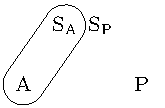
\includegraphics[\width=\linewidth]{figures/alignment}


\section{Phonology}
Vamale’s consonant and vowel phonemes are shown in Table \ref{tab:intro_cons} and Figure \ref{fig:intro_vowel}. As is typical of the area, there are many consonants, including labiovelarized and aspirate ones. Voiced plosives are pre-nasalized, and historical geminates have become ``fortis" consonants, either voiceless or aspirated plosives, or voiceless nasals and liquids. They attract stress and tend to nasalize the following vowel: [kʰɛ̃kʰɛ̃] \qu{parrot}, /han/ [hãn] \qu{to go}. 

%\begin{table}
%	\caption{Consonants in Vamale. Non-phonemes are in brackets.}
%	\begin{tabular}{p{1cm}lp{1.4cm}lp{1.2cm}lllp{1.2cm}l}
%		\lsptoprule
%		& Bilabial & Lab. Bilabial & Labiod. & Lab. Labiod. & Alv. & Palatal & Velar & Lab. Velar & Glott. \\
%		\midrule
%		Plosive & pʰ p ᵐb & (pʰʷ) pʷ ᵐbʷ &  &  & tʰ t ⁿd & (cʰ) c ⁿɟ & kʰ k ᵑɡ &  &  \\
%		Nasal & m̥ m & m̥ʷ mʷ &  &  & n̥ n & ɲ̊ ɲ & (ŋ̊) ŋ &  &  \\
%		Tap%or Flap
%		&  &  &  &  & (ɾ) &  &  &  &  \\
%		Fricative &  &  & f v & fʷ vʷ & s &  & x ɣ & xʷ & h \\
%		Approx. &  &  &  &  &  & j &  & w &  \\
%		Lat. Approx. &  &  &  &  & l l̥ &&&&\\
%		\lspbottomrule
%	\end{tabular}

%\end{table}

\begin{table}
\caption{Consonants in Vamale. Non-phonemes are in brackets.}
\begin{tabular}{llllllllll}
\lsptoprule
                   & Bilabial & Lab. Bilab. & Labiod. & Lab. Labiod. \\\midrule
Plosive            & pʰ p ᵐb & (pʰʷ) pʷ ᵐbʷ &           &              \\
Nasal              & m̥ m     & m̥ʷ mʷ        &           &            \\
Tap                &         &              &           &              \\
Fricative          &         &              & f v       & fʷ vʷ        \\
Approximant        &         &              &           &              \\
Lat. Approx.       &         &              &           &              \\\midrule
                   & Alveolar & Palatal & Velar & Lab. Velar & Glott. \\\midrule
Plosive            & tʰ t ⁿd & (cʰ) c ⁿɟ & kʰ k ᵑɡ &    &  \\
Nasal              & n̥ n     & ɲ̊ ɲ       & (ŋ̊) ŋ   &    &  \\
Tap                & (ɾ)     &           &         &    &  \\ % or flap
Fricative          & s       &           & x ɣ     & xʷ & h \\
Approximant        &         & j         &         & w  &  \\
Lat. Approx.       & l l̥     &           &         &    &\\
\lspbottomrule
\end{tabular}
\label{tab:intro_cons}
\end{table}

\begin{figure}
	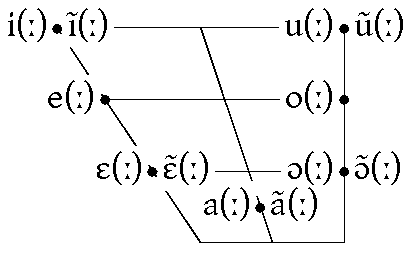
\includegraphics[width=0.4\linewidth]{figures/vowel}
	\caption{Vowel qualities in Vamale}
	\label{fig:intro_vowel}
\end{figure}


There are five phonemic vowel qualities /a, e, i, o, u/, with phonemic nasality and length: \textit{tha} \qu{assertive particle} \textit{thâ} \qu{excrement} \textit{the} \qu{algae} \textit{thê} \qu{rock} \textit{tho} \qu{call} \textit{thu} \qu{banyan tree}. The phonemic status of [ɔ̃] and [ũ] is a matter of analysis, as there are no minimal pairs with oral counterparts.

All vowels following nasal stops tend to be nasalized. There is limited allophonic variation in vowels, concerning chiefly /a/ pronounced [ɑ] after labiovelar approximants and /u/, which is pronounced [ʏ] after /i/, e.g. \textit{vwa} \qu{do} [vʷɑ], \textit{si-ung} \qu{hand-1\gl{sg}.\gl{poss}} [sʏŋ]. Possibly as a result of contact with neighbouring languages featuring more vowel phonemes, /o/ and /e/ have more open allophones in short closed syllables ([sɛn] \qu{poison}) or before a consonant in the same syllable ([ɔːt] \qu{rope, tendon, vine}), than in open ones ([ko] \qu{at}) or in long nasal-bounded ones ([soːm] \qu{swim}). Consonants may be lenited or fricativized in fast speech, and phonemically voiceless nasals and liquids may not be audibly realized as such (e.g. [m̥ũ̠ːn] $\sim$ [mũːn] \qu{smoke, dust}), but this is not a regular process.

Syllables never feature two consonants one after the other ((C)V(:)(C)), and may only end on a vowel, a nasal, or /p,t,c,k/, e.g. [tʰu] \qu{banyan tree}, [tʰuːp] \qu{bathe}, [tuːn] \qu{clan}. The early French loanword \textit{cheval} [ʃø.val] \qu{horse} was phonologically adapted to [so.van], as -l cannot occur syllable-finally.

Whether Vamale has true dipthongs (where both vowels occur in the same syllable) depends on the analysis. The second vowel in a syllable is always either /i/ or /u/ and not functionally distinct from the glides /j/ and /w/. Either Vamale has only dipthongs ending on /i/ or /u/, or Vamale has no diphthongs but may end the syllable on a glide. 

\begin{sloppypar}
The main stress is on the second-to-last (penultimate) syllable for most words, or on the first of three syllables, e.g. [ˈvʷaⁿ.di] \qu{peel by hand}, [ˈa.pu.li] \qu{person}. Vamale does not have native phonological words with more than three syllables: though morphologically speaking, there are longer structures, speakers split these up into intonational units of three syllables maximum, e.g. \textit{xa-vwa-tau} \qu{\gl{nmlz}-do-impact (fisherman)} is pronounced [ɣa.vʷa.ˈtau] but the four-syllable word \textit{xa-vwa-buke} \qu{\gl{nmlz}-do-flower (flower seller)} is pronounced [ˌɣa.vʷa.ˈᵐbu.ke].
Derivational prefixes, transitivity marking suffixes, possessive markers and other grammatical morphemes may behave differently stress-wise: bisyllabic morphemes may be counted as one stress unit, and some suffixes are even ignored completely, e.g.
\end{sloppypar}

\begin{itemize}
\item {[}ˈmu.lip] \qu{life}
\item {[}mu.ˈlip.ga.vwe] \qu{life-2\gl{pl}.\gl{poss}}
\item {[}ˈɲ̊i.mã] \qu{heart, thought}
\item {[}ˈɲ̊i.mã.ke] \qu{to think}
\end{itemize}

\section{Example sentences}

The example sentences have three different sources. The reference is given in brackets under the examples. Most of the examples were elicited or found in recorded free text (see \sectref{sec:Meth} for details on recording and transcription methods) and can be traced to an audio file via the FLEx database uploaded to ELAR. The text collection on FLEx can be ordered by ``Abbreviation". The abbreviations used correspond to the code of one or two letters and sometimes a number, and the number after the colon is the line in the text (e.g. AG1:394). Other examples were not audio-recorded, but noted in writing. Their references start by the date of the entry (e.g. 180722 p.93, or 07.11.18 p.93). Other examples were transcribed from audio files but not yet included in a Flex file, and are referenced by the filename and the time stamp, also on ELAR (e.g. vamale-181107.jpnelemwa-04: 00:00:30- 00:00:32). Unreferenced examples were constructed for the purpose of writing up the grammar, and checked with speakers. 

\section{Person forms and demonstratives} 

Vamale distinguishes subject (\gl{a}\slash\gl{S\textsubscript{A}}) and object (\gl{p}) person forms (\Cref{tab:intro_markers}). There are three numbers, singular, dual, and plural. The language distinguishes inclusive (\qu{us and you}) and exclusive (\qu{us but not you}) first person forms. Object pronouns are never independent as seen in (\ref{ex:intro_obj}), whereas the others may be attached to the verb or occur in a free form (\ref{ex:intro_both}). 

\begin{table} 
	\caption{Subject and object markers for active and stative verbs}
	\begin{tabular}{lllll}
		\lsptoprule
		& & cross-indexes & \multicolumn{2}{c}{pro-indexes}  \\\cmidrule(lr){3-3}\cmidrule(lr){4-5}
		&	Free form	& \gl{a}=/ \textsc{s\textsubscript{a}}= & -\textsc{s\textsubscript{p}} & -\gl{p}\\
		\midrule
		1\gl{sg} & \textit{io} & \textit{e=} & \textit{-o(ng)} & \textit{-o} \\
		1\gl{du}.\gl{incl}& \textit{gasu} & \textit{gasu=} & \textit{-gasu} & \textit{-kaeu}\\
		1\gl{pl}.\gl{incl} & \textit{gaa/gase} &\textit{ga(se)=}&\textit{-gaa}&\textit{-kaa}\\
		1\gl{du}.\gl{excl} & \textit{abu} & \textit{abu=} & \textit{-abu} & \textit{-(a)bu}\\
		1\gl{pl}.\gl{excl} & \textit{abe}& \textit{abe=} & \textit{-abe} & \textit{-(a)be}\\
		2\gl{sg} & \textit{go} &\textit{go=} & \textit{-go} & \textit{-ko}\\
		2\gl{du} & \textit{gau} & \textit{gau=} & \textit{-gau} & \textit{-kau}\\
		2\gl{pl} &\textit{gavwe}& \textit{gavwe=} & \textit{-gavwe} & \textit{-kavwe}\\
		3\gl{sg} & \textit{ia} & \textit{a=} & \textit{-(e)a} & \textit{-(e)a}\\
		3\gl{du} & \textit{lu} &\textit{lu=} & \textit{-lu} & \textit{-lu}\\
		3\gl{pl} & \textit{le} & \textit{le=} & \textit{-le} & \textit{-le}\\
		\lspbottomrule
	\end{tabular}
	\label{tab:intro_markers}
\end{table}

\ea[]{\label{ex:intro_both}
\gll e=xale-ko ka=yo\\
 1\gl{sg}=see-2\gl{sg}.\gl{obj} \gl{sbj}=1\gl{sg}\\
\glt \qu{I see you.}}
\z


\ea[*]{\label{ex:intro_obj}
\gll e=xale go \\
 1\gl{sg}=see 2\gl{sg}\\
\glt (for: \qu{I see you})}
\z

Most personal pronouns look similar to their free form counterpart, and were probably historically derived from them. Suffixes indexing objects and stative subjects (\gl{S\textsubscript{P}}) always refer to people or animals, whereas active subjects (\gl{a} and \gl{S\textsubscript{A}}) do not mark the animacy of their referent.

\ea
%\a
\gll phwaat i=thala\\
 clean \gl{def}.\gl{sg}=knife\\
\glt \qu{The knife is clean.}
\z

%\a
\ea
\gll a=tabo i=thala\\
 3\gl{sg}=sit \gl{def}.\gl{sg}=knife\\
\glt \qu{The knife lies (there).}
\z

The stative subject (\gl{S\textsubscript{P}}) and the object suffixes cannot co-occur with an independent person form (pro-indexing person forms).

Demonstratives distinguish number (singular, dual, plural) as well as proximity (proximal \textit{-hni}/distal (\textit{-na})). %Though they were probably transparently formed in the past, the current usage distinguishes the forms along more opaque lines: \textit{ena} is the only possible form useable to agree with a previous statement. 
The demonstratives resemble in part the articles, which are also listed in \Cref{tab:intro_demonstratives}. Two demonstratives, \textit{na} and its repeated form \textit{ha} (meaning it is used if the information is repeated, often with insistence), cannot be used as predicates, nor do they mark number or proximity: they are deictic pronouns that take a nominal predicate. They are illustrated in (\ref{ex:na}) and (\ref{ex:ha}).

\begin{table}
	\caption{Demonstrative pronouns and articles}
	\begin{tabular}{lll ll}
		\lsptoprule
		& \multicolumn{2}{c}{Demonstrative} & \\
		& \multicolumn{2}{c}{pronouns} &\multicolumn{2}{c}{Articles}\\\cmidrule(lr){2-3}\cmidrule(lr){4-5}
		& Proximal & Distal	&\gl{spec} and \gl{def}& \gl{spec} and \gl{indf}\\\midrule
		\gl{sg} & \textit{e-hni} & \textit{e-na}& \textit{i} & \textit{(e)ca}\\
		\gl{du} & \textit{muu-hni} & \textit{muu-na} & \textit{mu} & \textit{muca} \\
		\gl{pl} & \textit{ni-e-hni} & \textit{ni-e-na} & \textit{li} / \textit{ni} & \textit{ca(been)}\\	
		\lspbottomrule
	\end{tabular} 
	\label{tab:intro_demonstratives}
\end{table}

\ea
%\ea
\label{ex:na}
\gll na yo \\
 \gl{dem} 1\gl{sg}\\
\glt \qu{It's me.}
\z

\ea \label{ex:ha}
%a
\gll li=xa-vuki vai ko-n thexhwaade, {\ob}ha{\cb} {\ob}li=kalen{\cb}\\
\gl{def}.\gl{pl}=\gl{nmlz}-stem stone on-\gl{nspec} T. \gl{dem}.\gl{rep} \gl{def}.\gl{pl}=K\\
\glt \qu{The owners of Thexhwaade rock, are the Kalens (and no-one else).} {[DP:12]}
\z


\section{Element order}

Like many other Oceanic languages in the area, Vamale is predominantly VOS \REF{ex:vos}, though the pragmatically most important element (usually the subject) is frequently fronted \REF{ex:vos2}. Modifiers follow the modified, as in \REF{ex:vos1}.


\ea\label{ex:vos}
\gll le=fwii i=jamwa-m ka=li=mani\\
 3\gl{sg}=wake.up \gl{def}.\gl{sg}=father-1\gl{sg}.\gl{poss} \gl{sbj}=\gl{def}.\gl{pl}=bird\\
\glt \qu{The birds wake my father up.}
\z


\ea\label{ex:vos2}
\gll i=jamwa-m, go=fwi-a\\
 \gl{def}.\gl{sg}=father-2\gl{sg}.\gl{poss} 2\gl{sg}=wake.up-3\gl{sg}\\
\glt \qu{Your father, you wake him up.}
\z


\ea \label{ex:vos1}
\gll go=fwii i=jamwa-m a=meebam\\
 2\gl{sg}=wake.up \gl{def}.\gl{sg}=father-2\gl{sg}.\gl{poss} \gl{rel}=sleep\\
\glt \qu{You wake up your sleeping father.}
\z
\section{Argument coding}

Vamale has several strategies for argument coding. Its differences from those of Vamale's closest relatives, are likely due to contact with surrounding languages. (Pro)nominal subjects are marked differently from objects. As with all Northern New Caledonian languages, subject noun phrases of all verb classes are marked with dedicated (pro-clitic) particle, in this case \textit{ka}, e.g. (\ref{ex:active}), or \textit{a} when following a consonant-final word (e.g. \textit{a=soom a=ya} \qu{she=swims \gl{sbj}=she}). However, \textit{ka} \qu{\gl{sbj}} is optional and unusual for intransitive subjects, while it is obligatory for transitive ones. This is a tripartite alignment system as illustrated in \Cref{fig:intro_alignment1}, and found in other Voh-Koné languages as well. 

\begin{figure}
% % % 	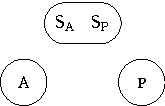
\includegraphics[width=0.3\linewidth]{figures/noun_alignment}
	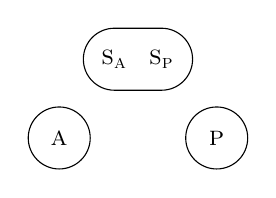
\begin{tikzpicture}
		\topleftnode[sa]{\gl{S\textsubscript{A}}}
		\toprightnode[sp]{\gl{S\textsubscript{P}}}
		\leftnode[a]{\gl{a}}
		\rightnode[p]{\gl{p}}
		\draw (a) circle (11.2pt);
		\draw (p) circle (11.2pt);
		\draw \convexpath{11.2pt}{sa,sp};
	\end{tikzpicture}
	\caption{Alignment of noun phrases}
	\label{fig:intro_alignment1}
\end{figure}

``Active verbs" may be either transitive or intransitive. They index transitive subjects \gl{a} identically to agent-like intransitive subjects \gl{S\textsubscript{A}}, and distinguish them from objects \gl{p}, as in (\ref{ex:active}). Another group of verbs, ``stative verbs", are always intransitive (\ref{ex:stative}), and mark the subject \gl{S\textsubscript{P}} similarly to undergoers in transitive verbs, but are distinct from them (see \Cref{tab:intro_markers} for the forms). %The distinction between \gl{S\textsubscript{P}} and \gl{p} forms is blurry depending on the speaker, and may in time disappear. The distinction is not found in western Voh-Koné where a strictly split-transitive system marks \gl{S\textsubscript{P}} like \gl{p} and like possessors as well, but instead the Vamale distinction mirrors the one found in Pije and Nemi spoken to the north of Vamale.
It is a tripartite system shown in \Cref{fig:intro_alignment2}, but differently so than the one for noun phrases.


	\ea
	%\ea
	\label{ex:active}
	\gll e=bune i=balô ka=yo\\
	 1\gl{sg}=steal \gl{def}.\gl{sg}=ball \gl{sbj}=1\gl{sg}\\
	\glt \qu{I steal the ball.}
	\z
	
	
%	\ea
	\ea\label{ex:stative}
	
	\gll xawe-ong ka=yo\\
	 young-1\gl{sg} \gl{sbj}=1\gl{sg}\\
	\glt \qu{I am young.}
		\z

	
\begin{figure}
\begin{floatrow}
\captionsetup{margin=.05\linewidth}
\ffigbox{%
% 	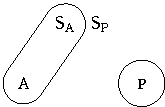
\includegraphics[width=0.3\linewidth]{figures/verb_alignment}
	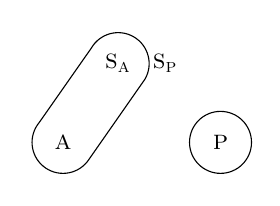
\begin{tikzpicture}
		\topnode{}
		\topleftnode[sa]{\gl{S\textsubscript{A}}}
		\toprightnode[sp]{\gl{S\textsubscript{P}}}
		\leftnode[a]{\gl{a}}
		\rightnode[p]{\gl{p}}
		\draw \convexpath{11.2pt}{a,sa};
		\draw (p) circle (11.2pt);
	\end{tikzpicture}}
	{\caption{Alignment with verbs}
	\label{fig:intro_alignment2}}

% % 	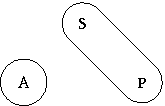
\includegraphics[width=0.3\linewidth]{figures/kan_alignment}
\ffigbox{%
	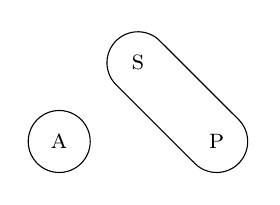
\begin{tikzpicture}
		\topnode[s]{\gl{s}}
		\leftnode[a]{\gl{a}}
		\rightnode[p]{\gl{p}}
		\draw \convexpath{11.2pt}{p,s};
		\draw (a) circle (11.2pt);
	\end{tikzpicture}}
	{\caption{Alignment with \textit{ka-n} nominalizations}
	\label{fig:intro_alignment3}}
\end{floatrow}
\end{figure}

This means that additionally to split-transitivity, which is common in the area, Vamale features a split along \gl{a}, \gl{S\textsubscript{A}}\slash\gl{S\textsubscript{P}}\slash\gl{p}. Some constructions, however, show yet different patterns: de-verbal nominalizations exhibit ergative alignment for inanimate subjects and undergoers, see (\ref{ex:intro_erg}) and \Cref{fig:intro_alignment3}. This last strategy is most likely related to possessive constructions, and uses similar morphemes (\textit{ka} and \textit{ka(-n)}, respectively). %It may have been calqued from a similar Cèmuhî construction, Vamale's neighbour to the south.
With active verb subjects (S/A-arguments), the cross-indexes occur under all circumstances, but with patient objects (P-arguments) and stative subjects, the pro-indexing suffixes cannot co-occur with the full nominal. 

\ea \label{ex:intro_erg}
\gll i=hun-coopwi ka i=vai\\
 \gl{def}.\gl{sg}=\gl{nmlz}-bury \gl{link} \gl{def}.\gl{sg}=stone\\
\glt \qu{the burying of the stone}
\z


\ea
\gll i=ape-tabo ka i=vai\\
 \gl{def}.\gl{sg}=\gl{nmlz}-sit \gl{link} \gl{def}.\gl{sg}=stone\\
\glt \qu{the position of the stone}
\z

\begin{sloppypar}
Ditransitive constructions distinguish human recipients from non-human ones; \textit{nya-si-} \qu{put-hand} is used for humans and \textit{nya-ko} for non-humans and humans in informal contexts alike. The markers can be discontinuous, as seen in \REF{ex:intro_nyasi_gift}. The constituent order is relatively free and subject to pragmatic preferences (compare (\ref{ex:intro_nyasi_demand}) and (\ref{ex:intro_nyasi_gift})).
\end{sloppypar}


\ea\label{ex:intro_nyasi_demand}
% \langinfo{}{}{} 
\gll e=ila-ke nyasi-m i=vai ka=yo\\
 1\gl{sg}=make.request-\gl{tr} \gl{ben}-2\gl{sg}.\gl{poss} \gl{def}.\gl{sg}=stone \gl{sbj}=1\gl{sg}\\
\glt \qu{I (politely) ask you for the stone (lit. I request the stone from you).}
\z


\ea\label{ex:intro_nyasi_gift}
% \langinfo{}{}{} 
\gll a=nya li=saleka-n si li=apuli\\
 3\gl{sg}=give \gl{def}.\gl{pl}=property-3\gl{sg}.\gl{poss} \gl{ben} \gl{def}.\gl{pl}=person\\
\glt \qu{He gives his things away to the people.} 
\z

\section{Word classes}

 Verbs can be sub-classified into free and dependent verbs, stative (i.e. state-like) and active (activity-like) ones. Nouns distinguish classifiers and different sub-classes nouns depending on their possessive morphology and ability to head a phrase. There are a number of subordinators, tense/aspect/mood markers, different kinds of pronouns etc. Typologically interesting aspects include the lack of a dedicated numeral class, whose function is instead covered by stative verbs, e.g. \textit{thaloo-lu} \qu{two-3\gl{du}} \qu{there are two, they are two}. There are no adjectives either, as is common in the area, where predicative adjectival functions are covered by stative verbs, and attributive ones by relative clauses, as seen in (\ref{ex:intro_pred}) and (\ref{ex:intro_att}).

\ea
\label{ex:intro_pred}
\gll vun-eo(ng)\\
 blue-1\gl{sg}\\
\glt \qu{I am blue.}
\z


\ea\label{ex:intro_att}
\gll a=thêên a i=thamo (a=) en maa-n\\
 3\gl{sg}=run \gl{sbj} \gl{def}.\gl{sg}=woman \gl{rel}= fine face-3\gl{sg}.\gl{poss}\\
\glt \qu{The beautiful (lit. `fine-faced') woman is running.}
\z

%\begin{table}
%	\centering
%	\caption{Main word classes}
%	\begin{tabular}{ll}
%		Main classes (that fill a unique slot) & Subclasses (based on morphosyntactic differences) \\
%		\midrule
%		\multirow{3}{*}{Nouns} & Alienable Nouns\\
%							& Inalienable Nouns\\
%							&Pronouns (personal, demonstrative) \\
%	
%		Articles &\\
%	
%			Subject proclitics		&\\		
%		TAM markers&\\
%		\multirow{3}{*}{Verbs}& Active Verbs\\
%			& Stative Verbs\\
%			& Manner Verbs\\
%		Adverbs&\\
%		Prepositions&\\
%			Subject marker \textit{ka}&\\
%		Conjunctions&\\
%		\multirow{3}{*}{Subordinators}&Complementizers\\
%		& Subordinators\\
%		& Relativizer\\
%		Negation markers&\\
%		Quantifiers&\\
%	\end{tabular}
%\label{tab:intro_wc}
%\end{table}

The negator \textit{cipa}, the assertive marker \textit{tha}, and epistemic mood markers such as the irrealis conditional \textit{cama} \qu{if ever} can precede both verbal and nominal (i.e. equational) clauses, see (\ref{ex:intro_clause}).

\ea \label{ex:intro_clause}
\gll tha cipa=le=hân\\
 \gl{ass} \gl{neg}=3\gl{pl}=go\\
\glt \qu{They did not leave.}
\z

\section{Verbs and verb phrases}

Verbs in Vamale are either free or dependent, meaning they may head a verb phrase or not. Serial verb constructions and other complex verbs are common and a productive way to express a series of related events, a complex action, or just to modify a verb.

Free verbs may take person-indexing proclitics (in the case of active verbs) or suffixes (for stative verbs), but usually omit them if in the imperative or prohibitive mood. The latter is marked by a particle \textit{cipii} (\ref{ex:intro_cipii}), related to the predicate negator \textit{cipa} (\ref{ex:intro_cipa}).



\ea\label{ex:intro_cipii}
\gll cipii (go)=see!\\
 \gl{proh} 2\gl{sg}=cry\\
\glt \qu{Don't (you) cry!}
\z

	
\ea\label{ex:intro_cipa}
\gll cipa=go=xaleke?\\
 \gl{neg}=2\gl{sg}=see\\
\glt \qu{Don't you see?}
\z


A set of particles precede the predicate to mark aspect and mood, as in \REF{ex:intro_bwa}. They can be combined, with sometimes idiosyncratic new meanings, and are sensitive to the verb's semantic nature (``aktionsart").
Their basic members are the imperfective \textit{bwa(n)}, perfective \textit{pa}, perfect \textit{ja}, progressive \textit{koon}, irrealis \textit{(b)o}, continuative\slash realis \textit{balan}, and frequentative\slash iterative \textit{mu}.

Verbs do not inflect for tense; indeed there are no dedicated tense markers, though the imperfective marker \textit{bwa} and the irrealis \textit{bo} are  used to suggest future actions (as in ex. \ref{ex:intro_bwa}), progressive \textit{koon} implies (relative) present tense and the perfectives \textit{pa} and \textit{ja} refer to the past. 

\ea \label{ex:intro_bwa}
\gll e=bwa=yahan\\
 1\gl{sg}=\gl{ipfv}=leave\\
\glt \qu{I will leave, I am just leaving.}
\z


\section{Derivation}

Many verbs are nominalized simply by putting an article before them, and some nouns can be verbalized by adding the transitive suffix \textit{-ke}. Indeed, entire verb phrases with arguments (but not tense or aspect markers) may be nominalized with an article. Other derivational affixes are the locative nominalizer \textit{ape-} (\textit{ape-tabo} \qu{place-sit; chair}), the manner nominalizer \textit{hun-} (\textit{hun-mata} \qu{manner-sing; singing style}), the instrumental \textit{e-} and the agentive \textit{xa-}. While \textit{e-} is ancient, others can be transparently reconstructed as former preposed nouns: \textit{ape-n} \qu{trace}, \textit{xa-} from \textit{xayu} \qu{man, male}. See (\ref{ex:intro_erg}) for two examples of nominalizers. 

\section{Nouns and noun phrases}

Nouns can be classified as inalienable (obligatory possessive morphology) or, if the morphology can be omitted, as alienable (see \Cref{tab:intro_PossSuffix1} for the suffixes). This follows a semantic logic, as is typical of Oceanic languages: inalienable nouns include kinship terms, body parts, and other parts of an individual (e.g. \textit{dedoo-ng} \qu{shadow-my}). Nouns can be possessed via direct (i.e. suffixal) or indirect (i.e. clitical) constructions, which usually depends on their alienability. However, a small number of nouns are alienable yet have directly possessed forms showing etymological stems: \textit{fedat} \qu{blood}, \textit{fedal-ong} \qu{my blood}. Nouns are either specific (using a definite or an indefinite article), or generic (without an article), as shown in (\ref{ex:intro_gen}). Number is also shown on the article instead of the noun. The only type of inflection found on nouns is adpossessive person marking (for animate possessors), and the formerly independent linker \textit{-n} indicating that the noun is possessed by a usually post-poned fully nominal possessor (\ref{ex:intro_poss}). Vamale has no adjectives; instead, nouns are modified via relative clauses. 


	\ea \label{ex:intro_gen}
	\gll i=xa-vwa i=xam\\
	 \gl{def}.\gl{sg}=\gl{nmlz}-do \gl{def}.\gl{sg}=mat\\
	\glt \qu{the maker of the mat}
	\z
	
	
	\ea
	\gll i=xa-vwa xam\\
	 \gl{def}.\gl{sg}=nmlz-do mat\\
	\glt \qu{the mat-maker, the maker of mats}
		\z


\begin{table}
	\caption{Possessive suffix paradigms}
	\begin{tabular}{llll}
		\lsptoprule
		&    & \multicolumn{1}{c}{inalienable} & \multicolumn{1}{c}{alienable}\\\midrule
\gl{sg} &	1&	\textit{-ng}&	\textit{-eong}\\
		&	2&	\textit{-m}&		\textit{-go}\\
		&	3&	\textit{-n}&		\textit{-ea}\\
		\midrule
\gl{du} &	1\gl{incl}&	\textit{-ju}&	\textit{-gaeu}\\
		&	1\gl{excl}&	\textit{-bu}&	\textit{-abu}\\
		&	2&	\textit{-u}&	\textit{-gau}\\
		&	3&	\textit{-lu}&		\textit{-lu}\\
		\midrule
\gl{pl} &	1\gl{incl}&	\textit{-je}&	\textit{-gaa}\\
		&	1\gl{excl}&	\textit{-be}&		\textit{-abe}\\
		&	2&	\textit{-vwe}&		\textit{-gavwe}\\
		&	3&	\textit{-le}&		\textit{-le}\\
		\lspbottomrule
	\end{tabular}
	\label{tab:intro_PossSuffix1}
\end{table}

\section{Possessive constructions and compounds}
An adpossessor nominal is unmarked (e.g. \textit{udee} in (\ref{ex:intro_poss})) and follows the possessed noun, which in turn carries a linker suffix \textit{-n} if the stem ends on a vowel, e.g. \textit{mwa-n}. 



	\ea\label{ex:intro_poss}
	\gll mwa-n udee\\	
	 house-\gl{link} medicine\\
	\glt \qu{pharmacy}
	\z
	
	\ea\label{ex:intro_poss2}
	\gll inya-m\\
	 mother-2\gl{sg}.\gl{poss}\\
	\glt \qu{your mother}
	\z

When the possessed noun is an inalienable term, it is marked for adpossessor person (see \Cref{tab:intro_PossSuffix1}, and (\ref{ex:intro_poss2})). Nominal compounds (\ref{ex:nom-comp}) are formally very similar to some nouns modified by relative clauses (\ref{ex:nom-rel}). However, the latter forbids articles in the modifying noun phrase, and the stress contours differ: a compound noun is treated as one unit instead of several. 


\ea\label{ex:nom-comp}
[iˌtʰamõˈxa.o.m̥ũ]\\
\gll i=thamo-xhaohmu\\
 \gl{def}.\gl{sg}=woman-elder\\
\glt \qu{the old woman}
\z


\ea\label{ex:nom-rel}
[iˈtʰaˌmõ ˈɣaˌsoːm]\\
\gll i=thamo (a= i=) xa-hnyimake\\
 \gl{def}.\gl{sg}=woman (\gl{rel}= \gl{def}.\gl{sg}=) \gl{nmlz}=swim\\
\glt \qu{the swimmer woman, the woman who swims}
\z

\section{Prepositions}

Vamale prepositions can be divided into prepositions proper (e.g. \textit{patemwano} \qu{very close by}) and ``relational nouns", which have nominal morphology and can sometimes be linked to a (voiced) nominal counterpart, see \Cref{tab:intro_prep}. 

\begin{table}
\caption{A selection of prepositions}
\begin{tabular}{l@{~}l  l@{~}l}
	\lsptoprule
	\multicolumn{2}{l}{Relational nouns}&\multicolumn{2}{l}{Related noun or meaning}\\
	\midrule
	\textit{cela-n}        & \qu{next to}                      & \textit{jela-n} & \qu{side}\\
	\textit{pwa-n}         & \qu{on top of}                    & \textit{bwa-n}  & \qu{head, top}\\
	\textit{can-hawâ-n}    & \qu{facing}                       & \multicolumn{2}{l}{in-face-\gl{link}}\\
	\textit{cake-bwa-n}    & \qu{on the other riverbank}       & \multicolumn{2}{l}{scoop.water-top-\gl{link}}\\
	\textit{cai-n}         & \qu{behind an animate entity}     & \textit{jèi-n} & \qu{back} (Cèmuhî)\\
	\textit{xala-n}        & \qu{under}                        & \\
	\textit{(can) dawee-n} & \qu{(in-) between}                & \\
	\textit{ca-n}          & \qu{in, at}                       & \\
	\textit{ko-n}          & \qu{on, at}                       & \\
	\textit{pathabua-n}    & \multicolumn{3}{@{}l}{\qu{before (spatial and temporal)}} \\
	\lspbottomrule         
\end{tabular}
\label{tab:intro_prep}
\end{table}

\begin{sloppypar}
Prepositions introduce adjuncts like points in time or locations, but also oblique noun phrases (\textit{nyako, nyasi}, see (\ref{ex:intro_nyako})), causes (\textit{ko}), adverbial clauses (\textit{can}), and subordinate clauses (\textit{ma, koma, cama}). %They are clitics, meaning they are syntactically own words, but do not carry stress. %yeah well there's ko,ma 'xaleke, 'canbwan, pwan 'jelan,jati etc
\end{sloppypar}

\ea \label{ex:intro_nyako}
\gll e=vi nyakoo-m\\
 1\gl{sg}=say \gl{obl}-2\gl{sg}.\gl{poss}\\
\glt \qu{I say (it) to you.}
\z

\section{Subordinate clauses}

There are relative clauses, adverbial clauses, conditional clauses, and, related to the latter, complement clauses. Relative clauses are the main way to modify a noun, adverbial clauses are one of the most important strategies to modify a verb, and many verbs require a complement clause. Relative clauses are introduced by the pro-clitic \textit{a}, probably related to the third person singular cross-indexing pronoun (\textit{a}), see (\ref{ex:intro_rel}). 

\ea \label{ex:intro_rel}
\gll li=dube a=xakoop(-le)\\
 \gl{def}.\gl{pl}=deer \gl{rel}=wild-3\gl{pl}\\
\glt \qu{the wild deer}
\z

Both the relativizer \textit{a} and the subject-indexing pro-clitic may be omitted (the latter only if the subject of the main clause is the same as the relative one). Subordinate clauses are formally identical to main clauses in both word order and content; only the subordinator marks the subordinate clause as such. Coordinate clauses are identical to subordinate ones except that that the subordinate clause may be fronted (\ref{ex:sub}), while coordinate clauses have a fixed order.

\ea \label{ex:sub}
\gll {\ob}ma le=tiike{\cb}, tha vwa ca=peipa la\\
 \gl{subr} 3\gl{pl}=write \gl{ass} \gl{exist} \gl{indf}.\gl{sg}=paper here\\
\glt \qu{For them to write, there is some paper here.}
\z

As shown in (\ref{ex:intro_can}), adverbial clauses are introduced by \textit{can}; contrary to other types of subordinate clauses, this type must omit the subordinate subject if it has the same referent as the main clause's. Complement clauses following verbs of opinion, speech, thought, etc are introduced by the complementizer \textit{hapi}, which developed from \textit{a=pii} \qu{s/he says} (\ref{ex:intro_hapi}). The other complement clauses follow either \textit{ma} \qu{with; if, when; in order to} (\ref{ex:intro_ma}), or, in more specific contexts, \textit{ko} \qu{because; on}, \textit{ko-ma} \qu{in order to}, and other particles. 


\ea\label{ex:intro_can}
\gll go=han {\ob}can pala kon yee{\cb}\\
 2\gl{sg}=walk  \gl{adv}.\gl{subr} talk \gl{obl}.\gl{nspec} tree\\
\glt \qu{You walk while talking about trees.}
\z

\ea\label{ex:intro_hapi}
\gll vaang {\ob}hapi na hmwaana{\cb}\\
 unknown \gl{comp} \gl{dem} like.this\\
\glt \qu{It is not clear that it is like this.}
\z


\ea\label{ex:intro_ma}
\gll nyima-m {\ob}ma go=pala{\cb}?\\
 will-2\gl{sg}.\gl{poss} \gl{comp} 2\gl{sg}=talk\\
\glt \qu{Do you want to talk?}
\z

%\section{Structure of this book}
%
%Writing a good grammar is a challenging task. Vamale has many forms with different, yet semantically related functions. For example, the repetitive particle \textit{mwa} can also mean \qu{again, in return}, \qu{on top of that, even}, as well as put the focus on one part of the clause and mean \qu{this here, now, here}. The grammars on Bwatoo \parencite{rivierre_bwatoo_2006} and Cèmuhî \parencite{rivierre_langue_1980}, as well as Isabelle Bril's extensive work on Nêlêmwa (\citedate{bril_nelemwa_2002}, \citedate{bril_noms_2004}, \citedate{bril_semantic_2005b}, inter alia), were of tremendous help and are frequently cited. 
%
%This thesis applies a classic descriptive structure to a language where syntactic behavior can be assigned to forms much more freely than in European languages: phonology, word classes, nouns and noun phrases, verbs and verb phrases, voice, aspect, and clauses. This means that some common words and constructions are introduced late in the book, and some relatively rare phenomena appear in the first chapters. Cross-references, an index at the back, and many small sections will help the reader find their way. In most cases, the examples presented were recorded, and can be found in their context either in the \href{https:www.elararchive.org/uncategorized/SO_d3953892-4107-4f7d-bcd2-cb36f44ba294/}{FLEx database} uploaded onto ELAR, in the field notes uploaded as scans, or in the .eaf transcriptions freely available along with their media files, also on ELAR.
%
%Chapter 2, '\nameref{ChapterContext}', is an alloy of the linguistic environment of the language and its genealogical ties on the one hand (along with a brief research history), and social, cultural, and historical information on the other hand, as well as some details on the main consultants and the research methods used on a third hand, with some general information on doing research in New Caledonia at the end. %This chapter basically unites most of the non-linguistic work in the grammar.
%
%The chapter \ref{ChapterPhon} on Phonology gives a description of the phonemes of Vamale, allophones, phonological rules, and syllable structure. A comparison to its most closely related relatives is made as well. Stress was investigated relatively late in the project, and the author cannot hope to give an exhaustive account, though the most important aspects are covered.
%
%Chapter \ref{ChapterWoCla} \qu{Word Classes} is a catalog of the syntactic behaviors of words in Vamale. As some classes only have one or two members, this chapter aims to dispense with labels that are all too clear, and moves along broad axes: first syntactic wordhood is discussed, then the distinction between verbs and nouns, which is especially important in Oceanic languages with zero-derivation. The chapter then groups the word classes by the constituents they depend on, though some particles must be discussed separately: \textit{mwa} \qu{again, also, even; now, here} and \textit{juu} \qu{real, very, only} modify a variety of domains, from words to clauses, and are discussed at the end. 
%
%The structure of the chapter \qu{Word Classes} is mirrored in the following chapters, grouping morphemes according to their constituent membership. \Cref{ChapterNouns} on nouns also includes classifiers and possessive constructions (\sectref{sec:Poss} and \sectref{sec:CL}, respectively), whereas \Cref{ChapterNP} \qu{Noun Phrases} takes up demonstrative suffixes again, as they are found on pronouns as well (\sectref{ssec:DemSuff}).
%
%\Cref{ChapterVerbs} \qu{Verbs} discusses the biggest word class in Vamale. Verbs come with a variety of syntactic behaviors: with numeral and adjectival functions, without a subject (\sectref{sec:ZeroTrans}), or unable to head a phrase (manner verbs and preverbs). The latter modify another verb and are described in \Cref{ChapterVP} \qu{Verb Phrases}. Nominalized verbs and verb phrases are described there (\sectref{sec:NomDeriv}), because their internal behavior is verb-like. Nominalized verbs are the only environment with ergative flagging: a particle \textit{ka} \qu{\gl{abs}} optionally flags inanimate \gl{s} and \gl{p} participants of nominalized verbs, but never agentive ones (\Cref{kan}).
%
%\Cref{ChapterVP} \qu{Verb Phrases} includes negators, serial verb constructions, and adverbs. Especially serial verb constructions are an important strategy to express complex events and to modify simple ones. 
%
%After a brief exploration of voice (\Cref{ChapterVoice}), especially of the middle prefix \textit{e-}, aspect is described in some detail in a dedicated chapter (\Cref{ChapterAspect}). Aspectual particles can combine and often have complex meanings, dependent on the predicate's aktionsart.
%
%Following the discussion of aspect, chapters on simple and complex clauses form the end of this description. While the chapter \ref{ChapterSimpClaus} \qu{Simple Clauses} includes a section on alignment, as well as one on modality, it mostly focusses on clause types. It covers declarative and imperative clauses, prohibitive ones, but also interrogative and even verbless clauses. The last chapter, `Complex Clauses', discusses coordinated and subordinated clauses (\Cref{ChapterSub}). Adverbial and relative clauses as well as the ones introduced by the important complementizer \textit{ma} are common constructions in Vamale. A brief section on insubordination closes the chapter, a construction used for adhortative, optative, and other modal ends. 
%
%Three texts form the appendix: a traditional fable as told by Mr.\ Philippe Gohoupe (\Cref{text:squid2}), an oral account of the 1917 Tipije War (\Cref{text:tipije}), and a text written by Mrs.\ Yvonne Sahilé which was translated by the workgroup (Mr.\ Jacob Oué, Mr.\ Nigai Kalène, and Mr.\ Christophe Pei) on the origin of dancing (\Cref{text:beat}). The traditional fable explains the importance of gratitude (and the animosity between squids and rats), the War account is a fascinating perspective on the devastating repression of the Koné-Tiwaka region a century ago, while Mrs.\ Sahilé's text is rooted in traditional motifs and tells of the origin of dancing.
%
%\begin{figure}[h]
%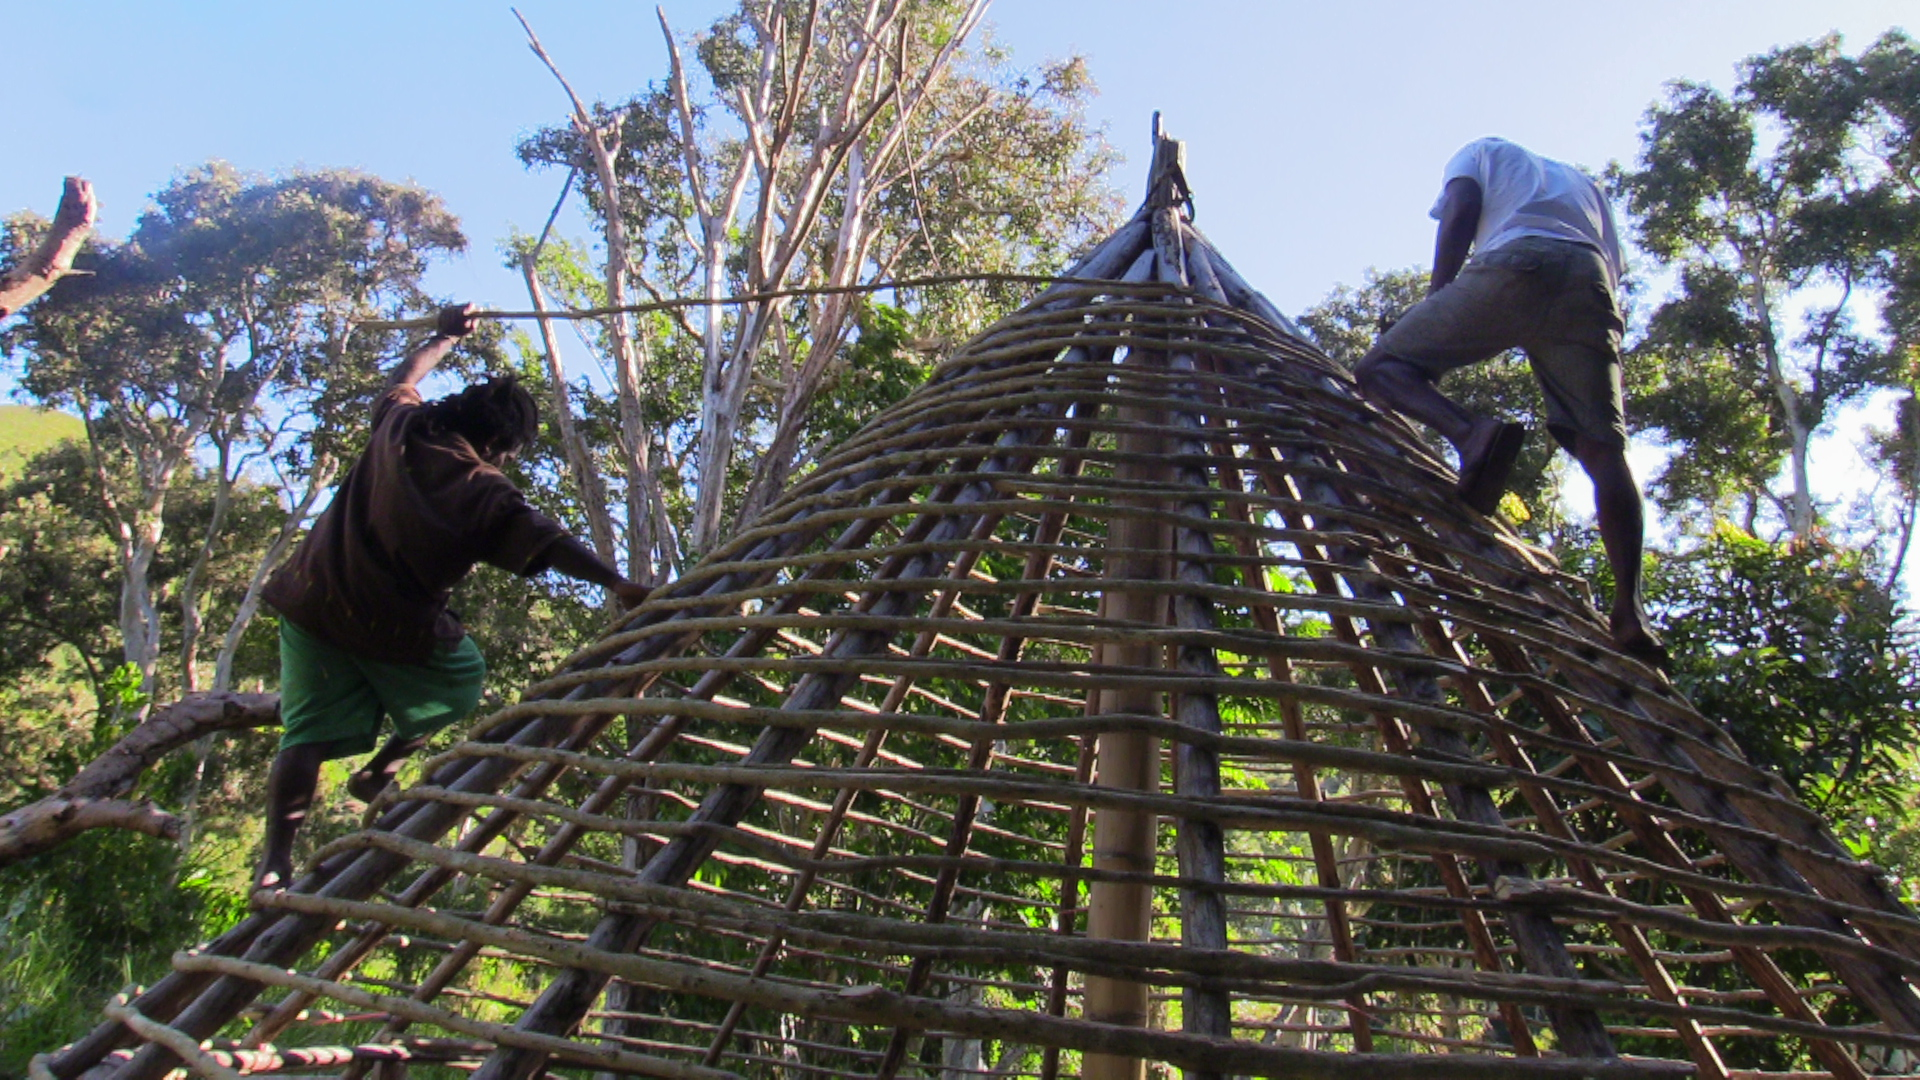
\includegraphics[width=\linewidth]{figures/house}
%\caption{Building a house requires many parts.}
%\end{figure}

\chapter{Methodology} 
\label{ChapterMeth}
\largerpage

\begin{sloppypar}
This chapter provides meta-information on our data collection, that is, that of the work group and me. It gives an overview of the methods used by us to gather the data discussed in the book. This includes the methods and thematic foci of data elicitation, the speakers we worked with in general and who the main consultants were, as well as some notes on climate and culture.
\end{sloppypar}

%\section{Methods}
\label{sec:Meth}

%Who the consultants were and their linguistic backgrounds and where they’re from in relation to all the stuff we already talked about and how great that whole thing was to be with them and  ... 


%In terms of educational background, I completed my MA in Language Documentation and Description at SOAS in December 2016. Along with a fieldwork class in Bern, the MA gave me a solid foundation and almost two years of experience in working with language data and speakers. In Bern and at SOAS, I had theoretical classes on linguistic, anthropological and methodological subjects.% I am familiar with the software I will use, with techniques of audio and video recording, and was sensitised to issues of usability and transparent data management. During this time, I have had the opportunity of working with all major types of recording equipment and to familiarize myself with the contexts in which to use them.
%The fieldwork course let me acquire theoretical knowledge and practical skills related to obtaining and analysing linguistic data. The courses involved designing, conducting and recording elicitation sessions with research participants, compiling a lexical
%database (in Toolbox and in FLEx), grammatical annotation through FLEx and ELAN (including morpheme-by-morpheme glossing), and finally translation of the data, as well as describing aspects of phonology, morphology and syntax of a language I was previously unfamiliar with. I am in grateful debt to my teachers. 
\section{Types of data recorded}

While the author hopes that this will not be the last work done on the language, this work attempts to give as comprehensive a description as possible. Since this may well be the last record of the language, and in any case the only one of Vamale as spoken in this period, the usability of the data is crucial. The work group recorded as much as possible, with members of every clan, spanning every generation but the youngest, and both genders (though a focus on males was hard to avoid for cultural reasons). We made videos of ceremonies, everyday activities, in Vamale as well as in other languages, and still missed hunts, funerals, and a women's craft week. The work group usually met three times a week and spent the entire day together. The days in between were spent transcribing and annotating, as well as preparing the next session. The elicitation sessions were usually structured in the following way: once the date, speaker, and location had been recorded, consent was established, and an overview of the topics of the day was given, in case a consultant wanted to avoid a certain topic. While the interviews with members of the local clans were conducted in Vamale as much as possible to avoid priming, the elicitation sessions with the work group most often featured questions and discussions in French, and answers in Vamale. Coffee, tobacco and food were provided by the researcher, along with customary gifts when meeting a consultant for the first time.

Data from transcribed data incorporated into FLEx carries references in the format L(L)(N):NN(N), e.g. KL:126, where the first part designates the text in the FLEx database, and the second the line number. Other data either shows the title of the audio recording and the time signature of the utterance, or the date and page of the notebook entry. Some data was overheard or so frequently used that no reference was given. 
%Most of this material remains untranscribed, and some recordings were not made due to fatigue of the researcher. Transcription, though initially planned to happen in the field, was mostly done in Bern using ELAN and FLEx. Description-wise, major gaps remain on prosody, and the semantics of some constructions. 

As explained in other sections (\sectref{ssec:Frenchpolicy}, \sectref{sec:Multiling}), there are few villages in the area that speak a single language, and Vamale is spoken exclusively in multilingual environments. French dominates in most places, but even where most people communicate in Oceanic languages, Vamale is almost never the majority language. This complex sociolinguistic situation is one reason for the relatively long period spent in the field, as every clan idiolect was recorded. The recordings are all marked for the speakers and place involved, leaving material for future research on language variation. 
A simple dictionary was compiled in the field using \citegen{leenhardt_langues_1946} wordlist and existing dictionaries of other languages as prompts, as well as the recorded data. Priming and misunderstandings were unavoidable, and language attrition contributed to the difficulties. Several elicitation sessions were dedicated to cross-checking this data and illustrating it with example sentences, and elders were visited explicitly to check old words. All materials are open-access and available online via the Endangered Languages Archive (ELAR), \href{https://elar.soas.ac.uk/Record/MPI1282765}{collection 0470}. The recorded data is also stored in the Archive of the Northern Province in Hienghène, as well as on SD cards left with the respective speakers. 

\section{Equipment used}
The project used the following equipment:

\begin{itemize} 
	\item Sennheiser headphones HD201, with a splitter to listen to recordings in groups
	\item Røde NTG-2 super-cardioid ``shotgun" microphone (a dead cat is appropriate on the coast due to the winds), and a Sennheiser EW122 lavalier microphone.
	\item a Canon XA30 camera, which can record audio in .wav format, has a powerful visual zoom, but a weak battery
	\item a Zoom H6 recorder
\end{itemize}

\section{Field trips}
A first field trip was undertaken in 2016, chiefly to ask for permission and support in the speaker area and from the relevant organizations: the Academy of Kanak Languages, the University of Nouméa, and the local customary authorities. This took two weeks, during which first lexicographical data were gathered. The research in 2017 lasted a little over 5 months, between June and December, the dry season. The first major stay was dedicated to gathering data from every speaker clan, and to do so in the form of stories and life recollections, as this was important to legitimize the project in the eyes of the speaker communities. The interviews were usually public, and several people would sit, listen, and occasionally chime in. I often mixed grammatical elicitation with text production, i.e. the first part would ask the consultants to check prepared sentences in Vamale or translate French ones, and the second part would invite them to speak about what they wanted. The latter part often revolved around the societal changes that occurred in their lifetimes, but some also commented on climate change, or narrated oral history. Most of these interviews were filmed as well, depending on the consent given (however, the camera battery gave out more than once in the first year). I also gathered botanical and zoological data and filmed people gardening and fishing, as well as building roofs and boats. Whenever possible, I participated in the activities I documented. The second field trip in 2018, around four months long, shifted the focus more to elicitation sessions, as the Bwatoo, Nêlêmwa, and Cèmuhî grammars were used as reference points to identify gaps in the description of Vamale. A third trip in 2019 focused on filling gaps, handing over data to the respective speakers (on SD cards, which was useless as most lack access to card readers; will be done differently next time), and transcribing as much as possible of the data gathered in the previous years. 

%rewrite the following. 

%

%The biggest villages, with an overall population of around 250, are Thewaade / Tiouandé, Thenganepaik / Téganpaik, and Wanaa / Ouanache. This is where most of the research took place, as it can take hours to the more remote settlements, and the roads are unreliable during rainy periods. 
%I budgeted enough SD-cards to be able to leave the data on them once recorded, thus already creating a card library. SSD harddrive disks will also receive the data as backup, and
Because of the amount of data recorded, time in the field did not allow for a complete transcription of the recordings. In order to alleviate the task, the author attempted to hire and train two locals to help him transcribe. This did not succeed as people were not used to sitting for hours, nor to working with computers. The most useful technique was to ask people to listen to the recording and repeat it clearly word for word for him to write down. This was particularly effective for the recordings of elders who were difficult to understand.

\section{Consultants} 
\label{sec:Consultants}
%This is how we will deal with this controversy and how we will name things in this volume which leads into discussion about ...Who the consultants were and their linguistic backgrounds and where they’re from in relation to all the stuff we already talked about and how great that whole thing was to be with them and 

Working on Vamale meant finding speakers willing to work with the researcher for free (except for transcriptions), in order to perpetuate the local custom initiated by French researchers. In exchange, consultants and speakers were welcome to discuss the goals of the project and change them. The project was assigned a team of three motivated representatives of the most powerful local clans. %Three friends of Dui 
Apart from the crucial fact that they had the time and the motivation to do it, they each had a different array of languages and social relations, which was very useful. From this nucleus grew a loose team of speakers joining in. The team members had lives and priorities of their own, and the group's makeup changed several times over the three stays. %This was partly tied to alcohol and personal problems on their side, a lack of cultural understanding on mine, and differences in our goals.

This section says a few words about the four main consultants. My deepest gratitude belongs to all of them. Other important people were Mr.\ Baptiste Ucian who kick-started the lexicon and most of the first months' elicitations, Mrs.\ Elise Kalène who gave a lot of her time to elucidate phonemes, and the entire population of the villages who were happy to share their views on the world, answer spontaneous questions, and always sympathetically asked how the work was going. 

\subsection{André Nigai Kalène}
Mr.\ Kalène is the eldest brother of Tiouandé's chieftain and grew up bilingual in Pije and Vamale. Extremely knowledgeable in traditions and a skillful boat- and house-builder, he was the most patient and reliable consultant and, in the beginning, walked an hour every day to our meetings. He has been politically invested in protecting indigenous rights his entire life. His extensive family network helped us tremendously.

\subsection{Christophe Keela Pei}

Mr.\ Pei is the herald of the powerful Pei clan, which housed and fed the author for ten months. Except for French, Mr.\ Pei is one of the rare monolingual speakers of Vamale, which helped decide whether a word was Vamale or a loan. Mr.\ Pei is a master fisherman and hunter. We often gathered at his house during the first research period.

\subsection{Jacob Keela Ganap Oué}

Mr.\ Oué is the eldest man in the land-owning clan of Wanaa and knows much about traditions, land ownership, and local history. A passionate gardener and ecologist, Mr.\ Oué spent time with Mr.\ Kalène rehabilitating mangroves, and is very knowledgeable about plants and animals. We spent most of our elicitations sessions at his house and he hosted the author for the last month. Mr.\ Oué speaks Vamale, Pije, and Fwâi, as well as excellent French. 

\begin{figure}
	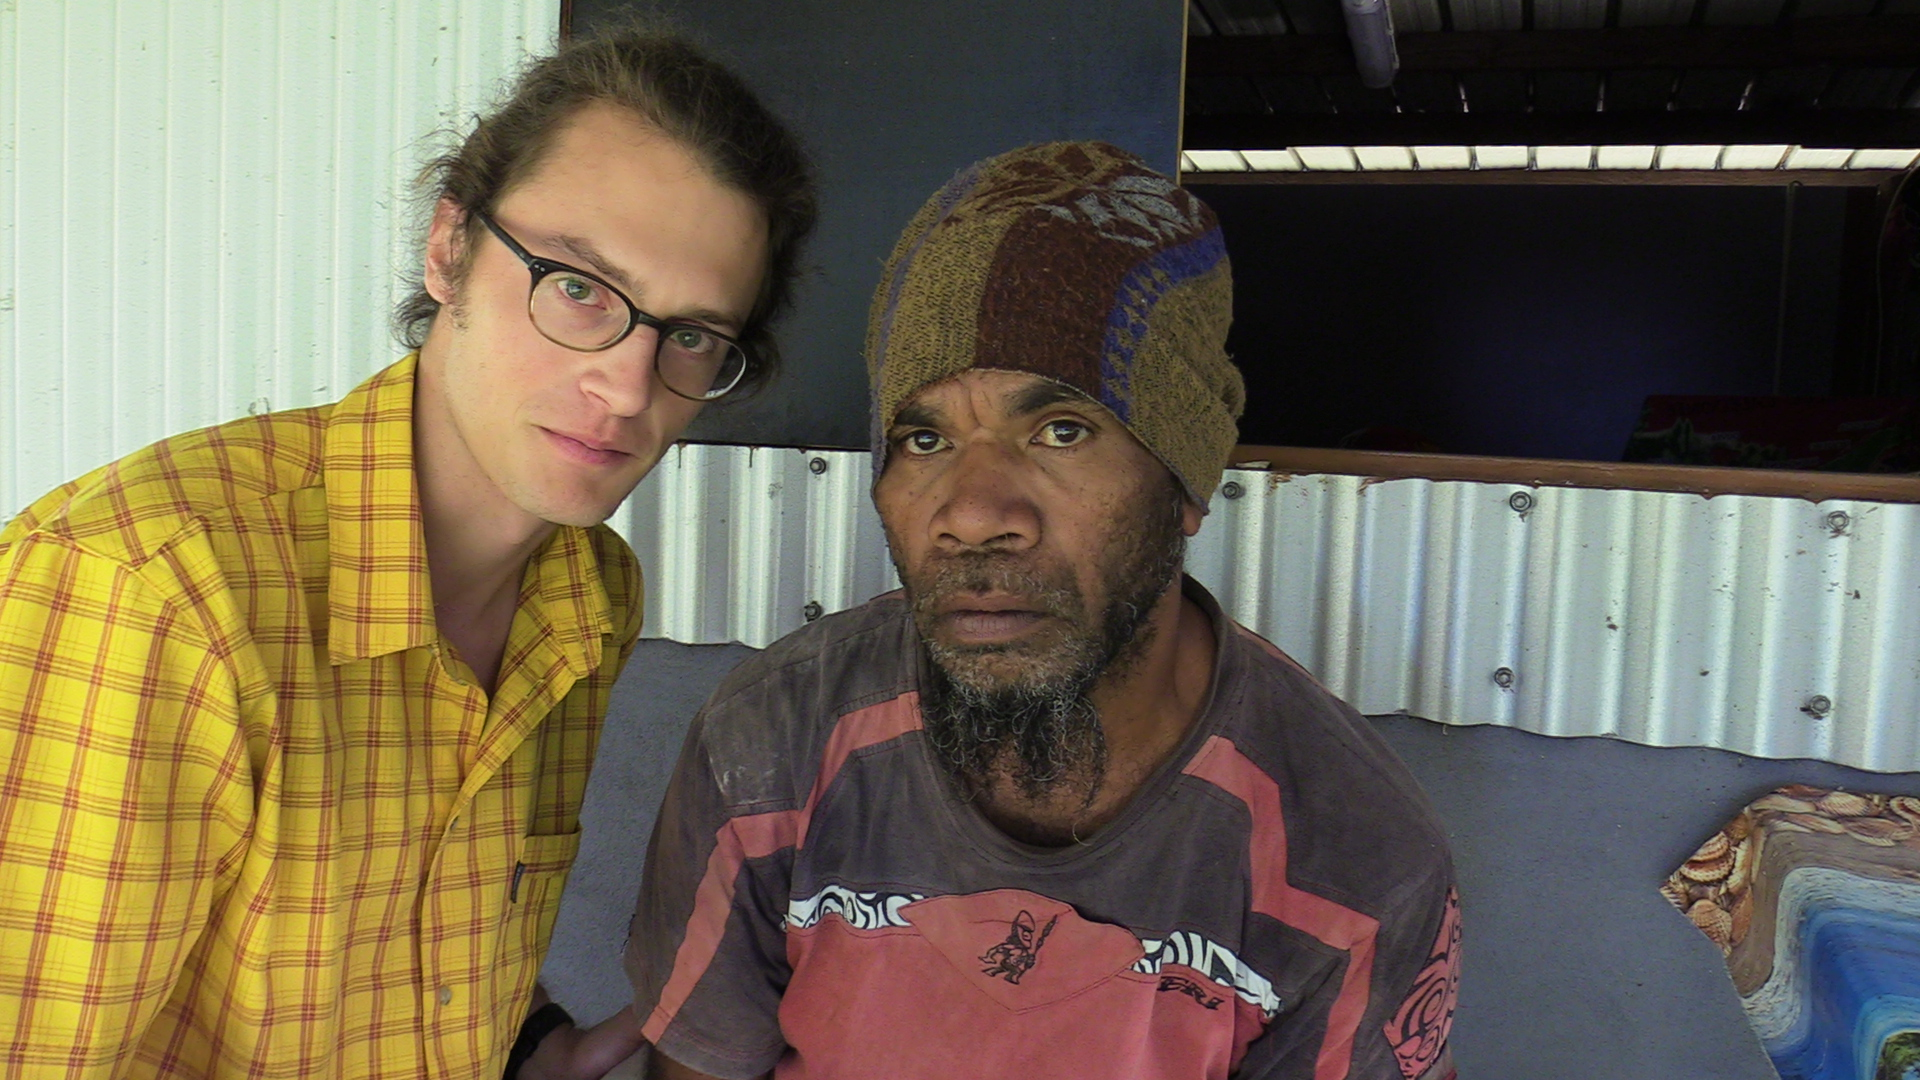
\includegraphics[width=\linewidth]{figures/gana}
	\caption{Mr.\ Jacob Oué and the author}
\end{figure}

\subsection{Jean-Philippe Emyl Téin Oué}

Mr.\ Oué was the only one in the group who was the author's age, and we spent a lot of time together in his garden, at his house, in his woods, and driving around. A speaker of Vamale, and able to understand Pije and Fwâi, he was the consultant most interested in syntax, morphology, and semantics, and spent many patient hours working on transcriptions, subtle differences between morphemes, and phonological questions.

The four men mentioned here guided the work through unspoken customs and laws, taught the author Vamale, and poured their time and hearts into the project. Without their help, most speakers would not have spoken to the author, nor would he have known where to go, and very little would have seen the light of day. \textit{Holeke thuan nyakoovwe ka gavwe i vaaya!}



\section{Notes on fieldwork in Vamale country}
\label{sec:Field}
%This section will refer to \Cref{ChapterContext} and \Cref{sec:Meth}, but does not seem redundant. While 
This work is a linguistic contribution, but some anthropological information is relevant for the reader to understand the cultural context in which the language is embedded, and some hints for future researchers may be useful. The northern east coast of New Caledonia is over 90\% ethnically Kanak, and everyday life is very much defined by this fact. % is not the easiest terrain to work in, and the culture is very different. %While this section try to avoid illusions about the interest of foreigners in working on this language, I hope that the following words will help anyone interested in working in the area, as well as shed some light on the problems I encountered.
%\subsubsection{2016, a sweating idiot.}
%This is a first description of the period between early November and mid-November 2016, which I spent with my then-partner Martha Amy Rose Newman in Téganpaïk. I am writing this from memory and it shall serve as a basis for a later section to be used in the dissertation.
%The east coast of Kanaky is a rainy, humid, warm area. %Grandma's digital watch has a broken thermometer that keeps claiming 30°C+ but it must be around 27-29°C. 
\subsection{Climate}
Although the temperature is relatively stable between 23°C and 28°C, humidity and sudden, unpredictable rain (even more so with climate change) can be dangerous for electronic equipment. The project used waterproof bags and silica gel packs to protect the equipment from humidity, and Lavaliers and hyper-directional microphones to mitigate the noise of the rain. Many roads become difficult when it rains, and most houses are tin-roofed, making recordings inside difficult due to echoes and rain/sticks falling on the roof. Noise from cars driving by on the main road was an almost unavoidable problem for recordings, though chickens took over that role wherever the setting was rural enough to exclude traffic.

%it is beyond me how people can walk for hours in the sun, a t-shirt wrapped around their head, or how they can play football. %I sweat. 
When it rains, it does so violently, and sometimes for days on end, with brief interludes. Tap water becomes murky, then brown, and finally stops working, so water-purifying pills are useful. Electricity may stop working if trees fall on the power lines. %A bucket fills in an hour. When it does not rain, it can remain dry for weeks. 
Because of the powerful weather, the obligation to attend ceremonies (especially unforeseeable funerals), the difficulty of planning an appointment etc., it is advisable to carry recording equipment at all times and record whenever possible, and to understand that plans can change at short notice. Life moves slowly, and people prefer to finish a thing properly to strictly adhering to an appointment. It may be frustrating to consultants to interrupt an interview, so it seemed preferable to keep the day planning flexible instead of \qu{making the most of it} and seeing three consultants in one day. 
% You never know when you meet a person again. % I prefer when it does not rain. Fish everywhere. Loris. Flowers that people in Europe would kill to be able to grow. Mangoes galore. Coconuts. Poingo bananas. 

\subsection{Lodging}
%Téganpaik is the home of Daniel Doui Péi, who worked at the city hall in Touho and thus became the first contact in the field. He housed the author and his partner on the first, exploratory trip in 2016, and later 
The author rented a small house from his first contact and stayed there for most of his time in the area. With the exception of old bachelors and widowers, the researcher was the only person in the village who had a house to themselves, slept alone in a room, and could retire to work whenever needed. On the other hand, this also alienated the author from the others and prolonged the time it took him to integrate into the community. It took approximately six weeks for the shyness to subside on both sides. The author still recommends individual housing, if at all possible. Participating in as many activities as possible helps bridge the gap between the community and the stranger, as recommended by Patience Epps for fieldwork in Hup country \parencite[37]{epps08hup}. %Dui's family fed him for most of his stay. 
Be aware of your imposition on a family, contribute in food and money so as to alleviate the burden you represent. Spend free, disinterested time with your consultants and family, as purely professional relationships hardly exist in a tribal setting. %(it is also nicer to be treated like a friend rather than an employer, boarder, etc).

People usually keep a Spartan interior, with little furniture except for beds, TVs, and an occasional table. Mostly, meals take place outside, where the kitchen tends to be located. In general, most people have little to no disposable income. Most families rely on the employment of a family member as well as their own gardens for subsistence. Customary ceremonies are a major part of life, and exchanging produce, clothing, and money in this context has a function of leveling inequalities: some people can only contribute bananas or fruit bats, but leave a ceremony with clothing, money and sugar. %Coming in with expensive equipment and being white makes one a potential source of revenue, which partly defines most relationships with locals. The author suggests acknowledging this by determining a budget that can be spent for others, and spending it light-heartedly.


%----------------------------------------------------------------------------------------
%	SECTION 2
%----------------------------------------------------------------------------------------

Some anthropological information is relevant to the reader. The northern East Coast of New Caledonia, uncontested \textit{Kanaky}, is not the easiest terrain to work in, and the culture is very different from Western contexts. I hope that the following words will help anyone interested in working in the area, as well as shed some light on the problems commonly encountered by Westerners in this country.

\subsection{Cultural notes}\largerpage
\label{ssec:Soc}
%before turning to more general information about (northern) Kanak society. 

Politically, traditional Kanak society is organized in family units headed by the father. The next bigger unit is the clan, to which all persons sharing a particular totem, or a common ancestor, belong. This is usually headed by the eldest male, though another elder may be chosen if the former works in the capital, for instance. Local clan branches send an elder (not necessarily the oldest member) to a clan council which makes the decisions concerning a community. The chief (or ``small chief") is either appointed or inherits his position, and represents the\is{Chiefdom} community in spiritual matters,\footnote{Part of this position is often held by the chief's younger brother, or the head of a lower branch of the chiefly clan. While the ``sorcerer" will lead the New Yam ceremony and perform incantations over the steam of the new year's first pot of yam (\textit{vwa bwa jadoon}), a ceremony which still happens today, he is not usually held responsible for changes in the weather or a failing harvest anymore, due to missionary influences.} but also to the great chief, %xxChief smol or big? and is his post a creation of the French?
whose authority stretches over several villages, and in some cases even covers whole islands  (e.g. Isle of Pines\slash Kunyié). The decisions by chiefs are supposed to be decisions made in consensus with all clan elders. This is relevant to fieldworkers as decisions regarding their research may take a long time, and access to speakers is usually negotiated through several layers. For example, one might need to first ask the regional customary council for permission, then the high chief, then the local one, and in rare cases the clan chief. As long as the customary road is followed, individuals will not refuse to work with outsiders. To save face, unwilling consultants will simply not be home at the discussed date. Trying to force them into showing up e.g. by getting the clan chief involved may work once, but is unethical.

The respect towards elders is a strong institution and, coupled with a reluctance to ask questions\footnote{This has two reasons: it could embarass the elder in case they do not know the answer, but more importantly, information is a wealth that is volunteered rather than asked for, like all forms of wealth in Kanak society. Refusing an offer or query is tricky for all involved, as it threatens face.} has made it difficult for heritage speakers to learn the language later in life. Face and shame remain powerful control mechanisms in Kanak society. Youths who make a mistake while talking will often be reprimanded, which discourages them even more from talking. \is{Gerontocracy}
Pedagogy traditionally consists of teaching-by-showing, or rather learning-by-paying-attention, which is mirrored in a reluctance to explain more than a small aspect at a time, and speaking quietly. Interrupting somebody is rude, and seniority plays a major role in turn-taking. Patience is paramount; many people willingly talk if the proper introductions were made and they are not rushed by questions.

Exogamous, virilocal marriage practices mean that in every traditional couple, the man is a local and the woman has moved from outside onto the land he inherited from his father \parencite[321]{salomon_hommes_2000}, although uxorilocal movements were attested in the late nineteenth century \parencite[89]{guiart_laire_1992}. This also means that every traditional couple is at least bilingual. However, since everyone in younger couples speaks French, many do not learn their spouse's language, choosing to communicate in French instead. This is one of the reasons for the decline in speaker numbers. \is{Exogamy}Speaking to the women is often useful, as they had to learn the language as well and may explain difficult concepts. Reanalysis and mistakes are possible, however.

Since every adult is supposed to raise offspring, adoptions are a common way of ensuring every household contributes to the\is{Adoption} perpetuation of the clan. Traditionally, one child goes back to the mother's family, to replace her and take care of the elders. Couples who struggle to have children may also ask for a child, and receive it soon after it is weaned. Families with too many children may give some away as well. In many cases, the children grow up close to their biological family and spend much time with their blood kin. As no terminological, or indeed salient cultural difference, is made between siblings and cousins, all members of the same ``generation" (formerly: the group that is initiated together, \textit{yidan}) descend from the same male ancestor and grow up together. The importance of parent-child relationships is thus somewhat lessened, and adoption less of a traumatic event than a Westerner might think. Outsiders' comments on adoption, land use, the role of women and other things are as unwelcome to the Kanak as they would be to anyone else, though curiosity is generally tolerated.

The traditional social hierarchy is \textit{de iure} still salient, as the customary authorities have the backing and acceptance of the State \parencite[2]{demmer_nationalisme_2003}. However, the chiefs' authority is not undisputed. This likely has different reasons, including the current chiefs' ancestors being installed by colonial forces \parencite[3]{demmer_nationalisme_2003}, which results in a hereditary system more rigid than what is described by Guiart for pre-colonial societies \parencite[5,8]{guiart_lorganisation_1954}. \is{Chiefdom}This is relevant because relying solely on the chief to organize research participants may exclude non-loyal residents, and introduce blind spots and complex jealousies. Pastors tend to have more unanimous prestige. %Apart from gendarmes, the medical staff in Touho and the clerk in the pharmacy, I saw no pupwaale. There are some Caldoches in the area, and a man called Martin who is as long-haired and bespectacled as me and works for the forestry department.
The adoptions, dispersals of clans, feuds between different people, confessional differences, language diversity, and stark contrasts in the access to public transportation (and stable roads) make the social web extremely complex. Being instrumentalized is unavoidable and rarely detrimental to the project. This complex web also means that one is quickly known, word-of-mouth is fast and effective, and interested parties will often join a workshop or an activity by themselves.%Néa Galé is an adoptive member of the Néa clan, lives in Baco, comes from Wanaa, moved out following an argument with his adoptive brothers.

Ceremonies occupy a central part of speakers' lives. They frame historical commemorations, some sporting events, and most cultural gatherings. All weddings, birth celebrations and funerals still follow traditional patterns, with ceremonies at every step. In all cases, the custodians of the land will receive symbolic gifts from the guests, and speeches in the native language will be held (comprehension is not required). This is one of the domains in which Vamale is not likely to be replaced by French as long as there are still fluent speakers. It is recommended to attend as many cultural gatherings as possible and to participate in preparing the location, the food, etc. Willingness to work (\textit{vapula}) is highly valued in Kanak society, as is tending to a garden, sharing wealth, and being parsimonious with speech.

There is widespread distrust of outsiders% (chief of Touho Mission: ``yeah you just snoop around and write your thesis, without understanding us. If you ever want to know what's really going on, come see me.")
, but this usually subsides after a conversation or two. Though the author never met any negative views against his person, his presence as a European scholar was regarded critically by some, and even bemoaned by Mr.\ Philippe Gohoupe. It helps to be accompanied by a local when visiting people for interviews.% \todo{have a look at this again later}

\subsection{The place of language in Kanak culture}
\label{sec:CultContext}
\is{Language and land}
Kanak identity is tied to language \parencite[29]{lynch_oceanic_2002} and land \parencite[91]{bensa_political_1997}. Similarly, an individual's paternal language is linked to their land tenure \parencite[40]{sallabank_language_2015}. The emphasis in the literature is often on the clan name, inherited from the father, and the accompanying land rights. This is also the case in everyday discourse. The language used changes according to need (see \sectref{sec:Multiling}), and people moving to a new place will usually adopt the local language. While this is considered polite, there is also a deeper function: strangers and newcomers have reduced speaking rights at the council and a lower social status. In modern society, with written land tenure records and weakened land master clans, being a newcomer also often means having no land. However, traditionally, especially in the post-1774 period, geographical mobility often went hand-in-hand with a change of name to get land rights \parencite[92]{bensa_political_1997}.
Identity is a complex matter nowadays. \textit{Métissage}, \qu{racial} mixture with descendants of Kabyls, Europeans, Polynesians, but also from other Kanak nations, is a factor as much as traditional values such as where one plants their yam or to which clans one is related. In an increasingly complex society, being \textit{juu} \qu{real} is also negotiated through speaking the language.\is{Language and land}
Nowadays, young people (who often do not speak their heritage language) refer to themselves via the name of their village or their community in graffiti, tattoos, on Facebook, etc. Older people will relate through clan ties, but especially Pije and Vamale are so small, due to a shared history, that speaking them unites people.

\section{Language name}
\label{sec:LanguageName}

%\textbf{ Social, political, geographical, and linguistic context of this study where we will now recall how “Vamale” is a complicated term because there’s a bunch of dialect stuff happening and naming practices which we list them here. Reminder we are focusing on THIS area which has the following villages where the following languages are spoken and this is how they interact with each other/their contact situation and this is where we can maybe talk about their similarities and differences which has implications for what language is what language and what we consider the language we’re focusing on in this study and}

The language described in this book has been called \textit{'Moaeke} \parencite{leenhardt_langues_1946}, \textit{Hmwaeke} (especially in Anglophonic literature), or \textit{Vamale}. A language called \textit{Hmwaeke}, or \textit{Fa Tieta}, is spoken in Tiéta, and is a very close relative of \textit{Vamale}.  
In the Kanak conception, languages are defined via the area they are spoken in \parencite[40]{sallabank_language_2015}. Although some broader terms are used, such as \textit{thiie} \qu{Cèmuhî}, \textit{vije} \qu{Pije}, or \textit{cî/thî} \qu{Paicî}, one's own language is often just called \textit{juu fati} \qu{real/indigenous language}, or \textit{fati-je} \qu{our language}. Dialectal differences within one's own language are described as \textit{li vataan geen fati} \qu{the different voices/accents of language}, or simply as \qu{the language of X}. As mentioned in \sectref{ssec:haeke}, maintaining a dialect's individuality is important to speakers. Whether the idea that there are ``true, correct" languages is new or not, distinctions are nowadays made between the ``real" \textit{Vamale} and the \textit{Vamale} of, say, Usa, or Tiéta. This was never mentioned in a derogatory way, as each family is understood to have its own influences and language histories. The mutually intelligible variety spoken in Tiendanite by descendants of refugees from Usa will thus be called \textit{Vamale Usa}, as they call themselves \textit{Vamale} speakers. Speakers of \textit{western Voh-Koné} varieties do not use the term \textit{Vamale}, as it is tied to the specific valley of origin. Speakers of other languages often use one term for all the \textit{Voh-Koné} varieties, calling them e.g. ``\textit{Vamale} of the other coast". The names \textit{Haake, Haeke, Haveeke, Hmwaveeke, Hmwaeke} are all derived from the greeting ``How [are you]?" and were given for the sake of naming. 
However, though the names suggest only slight dialectal differences, \textit{Haeke} is not easily understood by \textit{Vamale} speakers, nor do the respective speakers consider themselves to speak the same language (albeit acknowledging their similarities). Each community having their own speech is especially important to people who had a different history than the other speech communities, as the last hundred years have strongly contributed to the identity . 


Naming the language after its place and not a distinctive feature that ties it to the dialect cluster is closer to peoples' own conceptions, namely that they are defined by their geographic origins and share more with the east coast than the west coast. \textit{Vamale} speakers do not consider themselves to form a cultural unit with other speakers of \textit{Voh-Koné} languages, preferring to identify with their three home villages, their commune Touho, and in general the east coast of the northern province. Since this is not a region that has a name useable for our purposes, the historical origin, Pamale \goodtilde Vamale, used by the speakers, seems appropriate. Apart from differences in phonology, lexicon, syntax, society and linguistic context, there is also a political reason to call this language \textit{Vamale} instead of \textit{Hmwaeke}.

\textit{Voh-Koné} is a cluster of varieties that are called dialects in the literature. This means that their speakers are counted as a unit, and amount, together, to over 1,000 people, which makes them seem a robust language group. However, most of these varieties, except \textit{Haveke}, have few young speakers and are thus endangered. Labeling them ``dialects" and not ``languages" has hindered efforts to protect them, as the former concept enjoys less prestige than the latter. While many people acknowledge that \textit{Cèmuhî}, and \textit{Paicî}, are languages with a grammar and a literary tradition, the author was told by Kanaks and Europeans alike that \textit{Vamale} was a waste of time, as it had no ``grammar". Without going into more detail, this book will usually refer to \textit{Vamale} as a language, or a variety, but avoid the word ``dialect". %It will treat Usa similarly, because mutual intelligibility is not sufficiently salient grounds for its speakers to group them together

If \textit{Vamale} is ever to be taught at school in Touho, it must be recognised as a language separate from \textit{Haeke}, which is already an official language of schooling in the cultural \textit{aire} Paici-Camuki. Crucially, \textit{Haeke} is only taught in the Koné area. The separate status of Vamale, and its emplacement on the east coast, was recognized by the cultural bureau in Pwäräiriwâ (Ponérihouen) in 2019. Finally, since \textit{Vamale} is called \textit{Vamale} and not \textit{Hmwaeke} by its speakers and their neighbors, this book will keep to their own usage.

%, nor to the survival of the varieties concerned.
%Language vs dialect and the consequences of this difference (funding, description, local attitudes)

%\begin{comment}
%\subsection{2016, a sweating idiot.}
%This is a first description of the period between early November and mid-November 2016, which I spent with my then-partner Martha Amy Rose Newman in Theganepaik. I am writing this from memory and it shall serve as a basis for a later section to be used in the dissertation.
%The east coast of Kanaky is a rainy, humid, warm area. Grandma's digital watch has a broken thermometer that keeps claiming 30°C+ but it must be around 27-29°C. Everybody moves slowly, it is beyond me how people can walk for hours in the sun, a t-shirt wrapped around their head, or how they can play football. I sweat. When it rains, it does so violently, and sometimes for days on end, with brief interludes. The water stops working, electricity may stop working, TV may be down. A bucket fills in an hour. When it does not rain, it can remain dry for weeks. I prefer when it does not rain. Fish everywhere. Loris. Flowers that people in Europe would kill to be able to grow. Mangoes galore. Coconuts. Poingo bananas. 
%People don't have a lot of stuff in their houses, some do not seem to wear shoes often, or have many clothes to change (most people do change their clothes often).
%Apart from gendarmes, the medical staff in Touho and the clerk in the pharmacy, I saw no pupwaale. There are some Caldoches in the area, and a man called Martin who is as long-haired and bespectacled as me and works for the forestry department.
%The adoptions, dispersals of clans, feuds between different people, confessional differences, language diversity, and stark contrasts in the access to public transportation (and stable roads) make the social web extremely complex. Néa Galé is an adoptive member of the Néa clan, lives in Baco, comes from Wanaa, moved out following an argument with his adoptive brothers.
%There is a distrust of white people (chief of Vieux Touho, or Touho Mission, don't remember: "yeah you just snoop around and write your thesis, without understanding us. If you ever want to know what's really going on, come see me."), a tradition of teaching-by-showing, or rather learning-by-paying-attention, which is mirrored in a reluctance to explain more than a small aspect at a time, and speaking quietly. I think this point needs more detailed explanation. Though I never met any negative views against my person, my presence as a white scientist was seen critically by some, and even bemoaned by Ao Cakeo. 
%
%Pei Dui's family, which comprises his woman from Maré, Élise (?) and his daughter whom he had with a Paicî woman and who is in a boarding school in Poindimié, Elodie, moved from a small concrete house now cluttered with stuff, mostly papers, next to the concrete foundation (a concrete disk with a hole for the central post) of a planned, or torn down hut, to an empty house uphill of his adoptive mother's house and his adoptive brother Richard's house, who has a roofless hut next to it, the straw for which has been dry in his garden since 2013. Dui's new house was built with subsidies, the surrounding ground is rubble, Yaté the dog would guard it if she weren't so sweet. 
%\end{comment}

\chapter{Language family, neighbors and previous work} % Main chapter title
\label{ChapterContext} % Change X to a consecutive number; for referencing this chapter elsewhere, use \ref{ChapterX}

\ea
\gll juu va m=e=juu saxhuti nyakoo-vwe i=jaxhut ko i=vamale...\\
 real too.much \gl{subr}=1\gl{sg}=real narrate for-2\gl{pl} \gl{def}.\gl{sg}=story about \gl{def}.\gl{sg}=Vamale\\
 \glt \qu{It is beyond me to properly tell you the story of the Vamale language...}
\z

This chapter aims to introduce Vamale in its genealogical context, as well as its current geographical environment. The language has been affected by its role in the area over time, its neighbors, and the contact situations born of that. Because Vamale speakers were one of the most severely impacted speaker communities of the 20th century in New Caledonia (see \chapref{chap:Tipije}), \textit{i vaa can vije}, the 1917 Kanak revolt or war, plays a crucial role in understanding why so few speakers remain, and why Vamale is a pluricentric language spoken by traumatized people. \chapref{chap:Tipije} summarizes the background and main events of this war.

Vamale is said to have approximately 100 speakers left \parencite{eberhard_vamale_2020}. Asking community members to list everyone capable of having a conversation in 2017 yielded 186 names, nine of whom have since passed away (as of January 2021). Worryingly, only 32 speakers are younger than thirty, and only 2 are minors. Most fluent speakers are over 60 years old. Though the language is used in ceremonies and some households (e.g. Téganpaik chief's house), and amongst many adult speakers, persons under 25 years of age barely use it with each other. A notable exception is the village We Hava, where a majority of residents understand, and many speak, the language. In one, maybe two generations, the language will stop being spoken, unless the trend is reversed. 
%The cultural focus on older males also reflects on the speaker census. When asked, most (male) speakers claimed that the women and children did not really speak it, which turned out to be an exaggeration. 81 of 180 speakers counted by a community member were women, though exogamous practices mean that they rarely stay in the village after marrying. 
On a hopeful note, an association was founded in 2019 with the goal of maintaining the language vital and promote its use (pictured in \Cref{fig:assoc}). Several workshops to this end have already taken place since the beginning of the research project, like the one shown in \Cref{fig:workshop}.

\begin{figure}
	\centering
		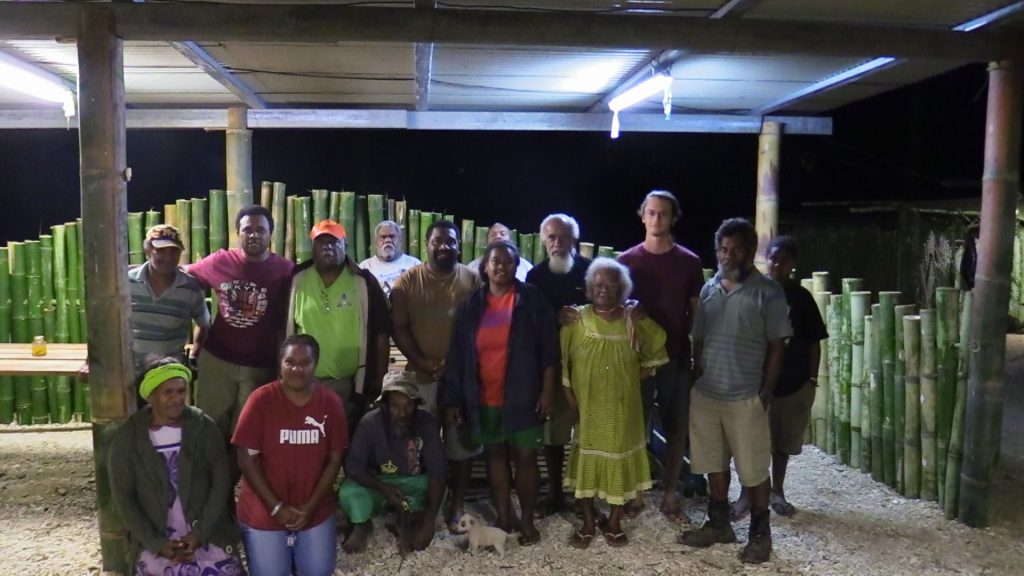
\includegraphics[width=\linewidth]{figures/assoc}
		\caption{The founding members of the Association Vamale.}
		\label{fig:assoc}
\end{figure}

	\begin{figure}
	\centering
	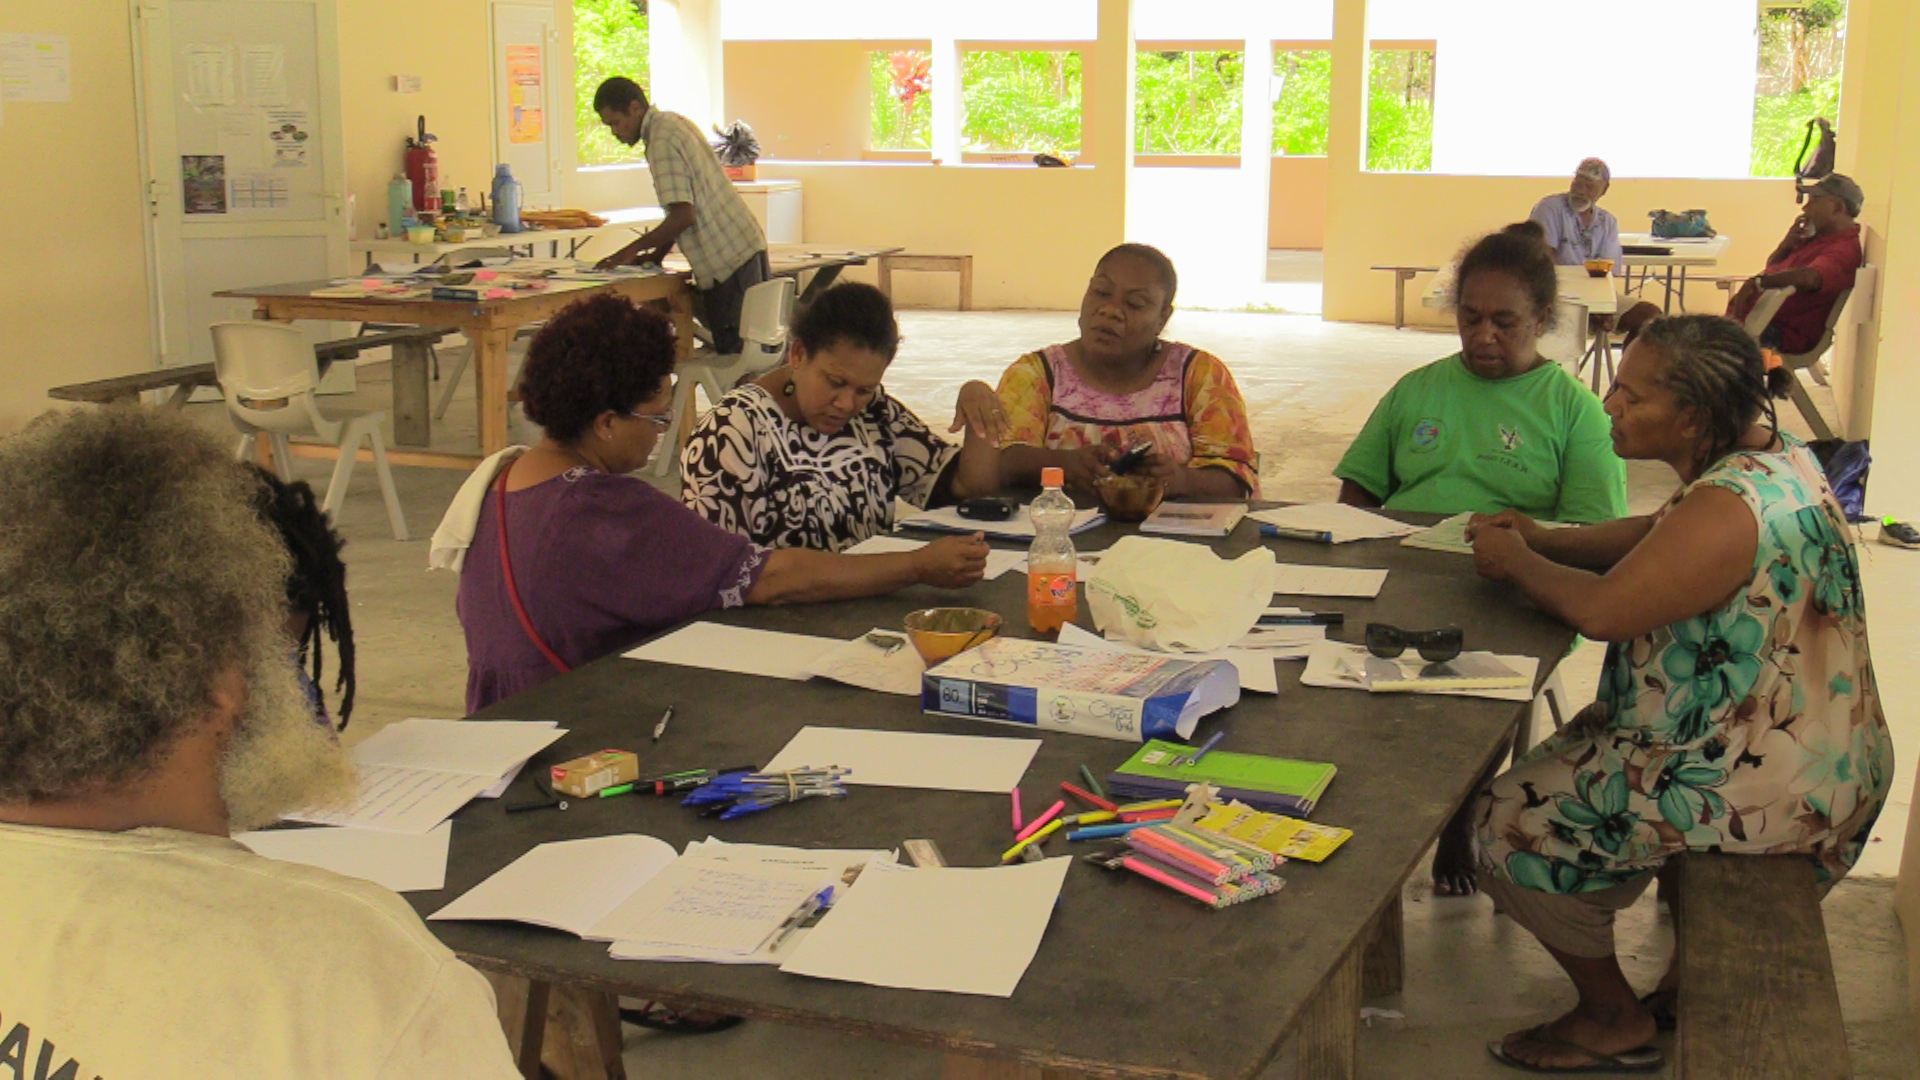
\includegraphics[width=\linewidth]{figures/atelier}
	\caption{A language workshop in late 2018, with members of the Academy of Kanak Languages.}
	\label{fig:workshop}
\end{figure}

%The chapter is structured as follows: first, the language is situated in the world (\Cref{sec:place}). The language's place in its family is discussed in \Cref{sec:Ling_Profile}. Previous work on the language is listed in \Cref{sec:prev_work}. \Cref{sec:Tipije} summarizes the events surrounding the war of 1917, while \Cref{ssec:Frenchpolicy} describes the circumstances leading to the language's decline after the displacement of the speakers. The section following this describes the situation of the language today: the villages in which it is spoken (\Cref{ssec:Geo}), the society which uses it (\Cref{ssec:Soc}), the cultural context relevant to language transmission (\Cref{sec:CultContext}) and code-switching (\Cref{sec:Multiling}), as well as Vamale's linguistic neighborhood (\Cref{ssec:neighbors}). The issue of the language's name is discussed in \Cref{sec:LanguageName}. A section on the main consultants introduces the work group and their linguistic background (\Cref{sec:Consultants}). The project's methods of data gathering are described in \Cref{sec:Meth}. Some information regarding doing fieldwork in New Caledonia closes the chapter (\Cref{sec:Field}).
 This section describes the situation of Vamale today. Below are brief descriptions of the villages in which most speakers live (Nouméa, the capital, is exempt), and a list of the languages found in the direct vicinity of Vamale. %The latter is important in the context of the name of this work's subject, and whether it is a dialect or not (see \sectref{sec:LanguageName}).


\section{Current geographical location of Vamale}
\label{sec:place}
Vamale is spoken on the northeastern coast of \textit{Grande Terre}, the biggest island in the archipelago of New Caledonia (\Cref{fig:SouthOceanic}). These islands, located south of Vanuatu in the subtropical Coral Sea, were settled around 3,200 years ago by Lapita sailors from Vanuatu \parencites[334]{lynch_efate-erromango_2004}[309]{sand_what_2007}. Contacted in 1774 for the first time by Europeans, the archipelago was formally claimed by the French in 1853, to break up British dominion in the area. French settlement, and the plantations tied to it, led to an influx of speakers of Vietnamese, Polynesian, Vanuatuan, and French varieties. Before this period, the islands hosted a family of at least 35 South Oceanic varieties\footnote{Leenhardt described 36 varieties, some of which are considered dialects of the same language, e.g. Orowe, Hamea, and Ajië. Given that in the 1940s, many of them were already quasi-extinct (e.g. Waamwang, Arhâ, and the ceremonial varieties of Drehu and Nengone), and given the catastrophic decline of the Caledonian population, \textit{and} how many small languages still co-exist in the North, a larger number may be presumed to have existed.} as well as a Nuclear Polynesian language spoken on Iaai/Uvea since the 17th century: Fagauvea (see \Cref{fig:SouthOceanic})
Vamale is the only member of the Voh-Koné linkage situated on the rainy east side of the central mountain range, about 375 km northeast of the capital Nouméa. The sea immediately to the east, and steep, sparsely populated mountains to the west mean that there is an about 5km large belt in which humans live in any density to speak of, and where Kanak languages are mostly found nowadays. Vamale is spoken in an area approximating 25 km\textsuperscript{2}, but apart from isolated houses like Laurient Gohoupe's far upstream of We Hava, the speakers can be found in five villages (and, of course, the bigger towns of the territory). These will be described in more detail in \sectref{ssec:Geo}.


\label{ssec:Geo}
%\begin{figure}
%	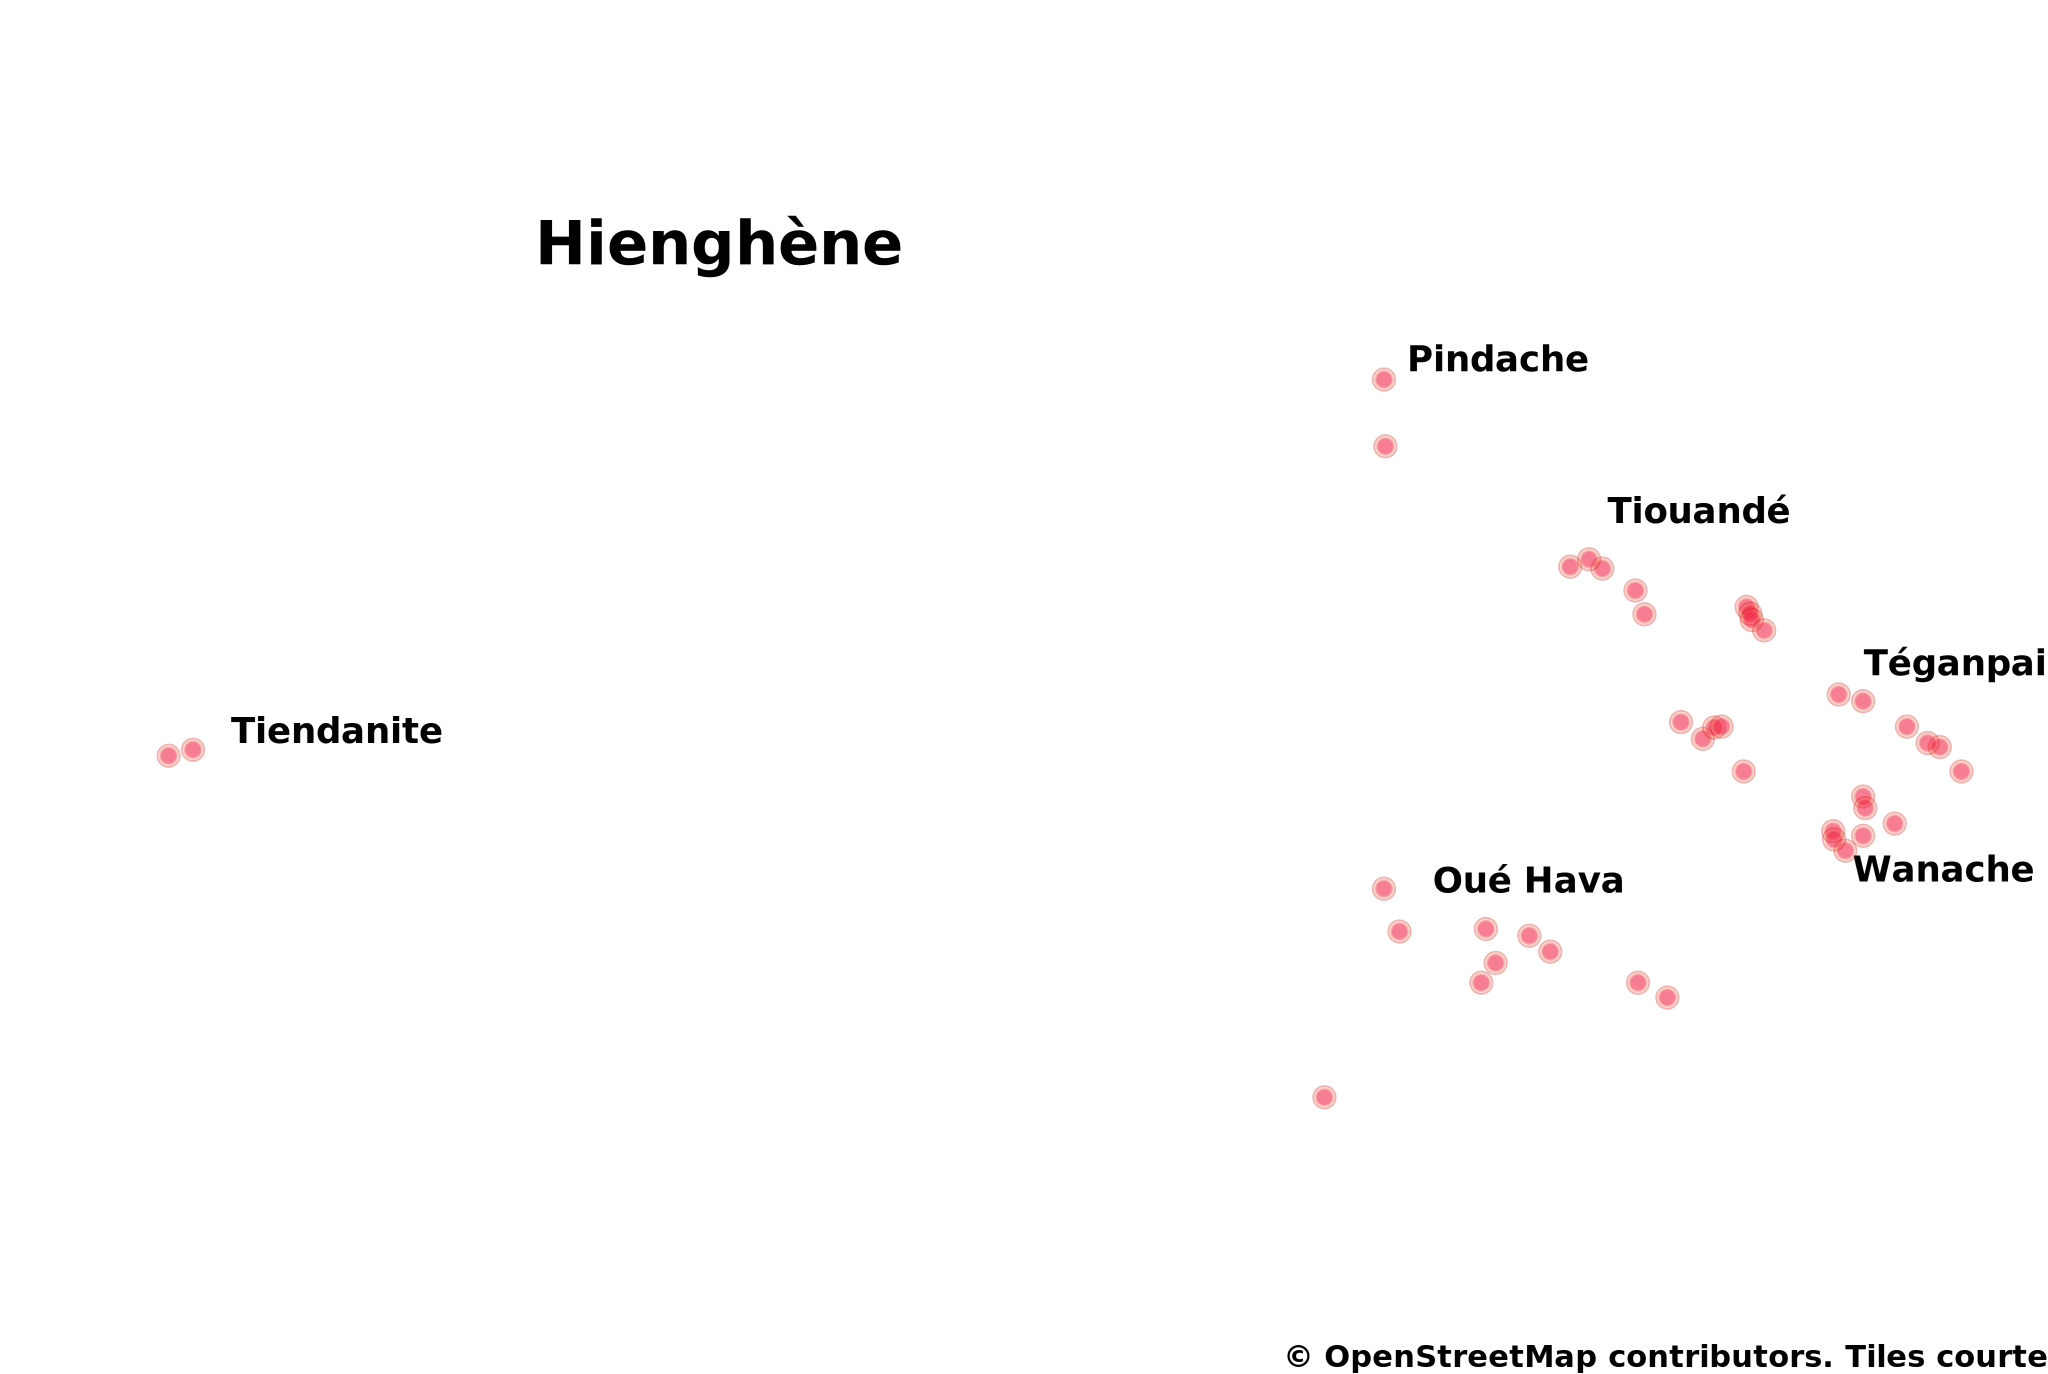
\includegraphics[width=15cm]{figures/map_dots}
%	%Gouvernement de la Nouvelle-Calédonie, 22-11-2017
%	\caption{Approximate map of speaker households on the east coast (Government of New Caledonia, 22.11.2017), dots are my own, thanks to Florian Matter.}
%	\label{fig:speakerMap}
%\end{figure}



%This documentation will produce one of the bigger corpora on New Caledonian languages, and may be a useful source in researching variation across time and space. For example, we have little knowledge of the history of Voh-Koné languages. Since they are concentrated between Voh and Koné on the east coast, and Vamale used to be spoken in the mountains, it is likely that they first settled in the mountains and then crossed them to the other side, but what the relation between the languages is, how and when they moved, and what the precolonial history of the area is, are questions more easily answered with comprehensive records of oral history, borrowings, and toponyms.
Vamale is spoken in several villages in the communes of Touho and Hienghène along the east coast of northern New Caledonia, in some villages in the mountains, and perhaps close to the west coast (Baco, Koné). The community is thus relatively widespread, which has given rise to a number of “family idioms”.
The Vamale-speaking area is large but sparsely populated, and concentrates on four villages. This work will usually prefer the word ``village" to ``tribe", which would be the translation of the official French term \textit{tribu}, because the Vamale word used for village, \textit{xhoogo}, means \qu{home} and has no connotation of a tightly-knit group of clans (especially since the 1917 war), and because it ultimately derives from a colonial vocabulary trying to establish a fundamental difference between Kanaks and settlers.
This section will thus describe the villages in which Vamale is spoken. 

\begin{figure}
	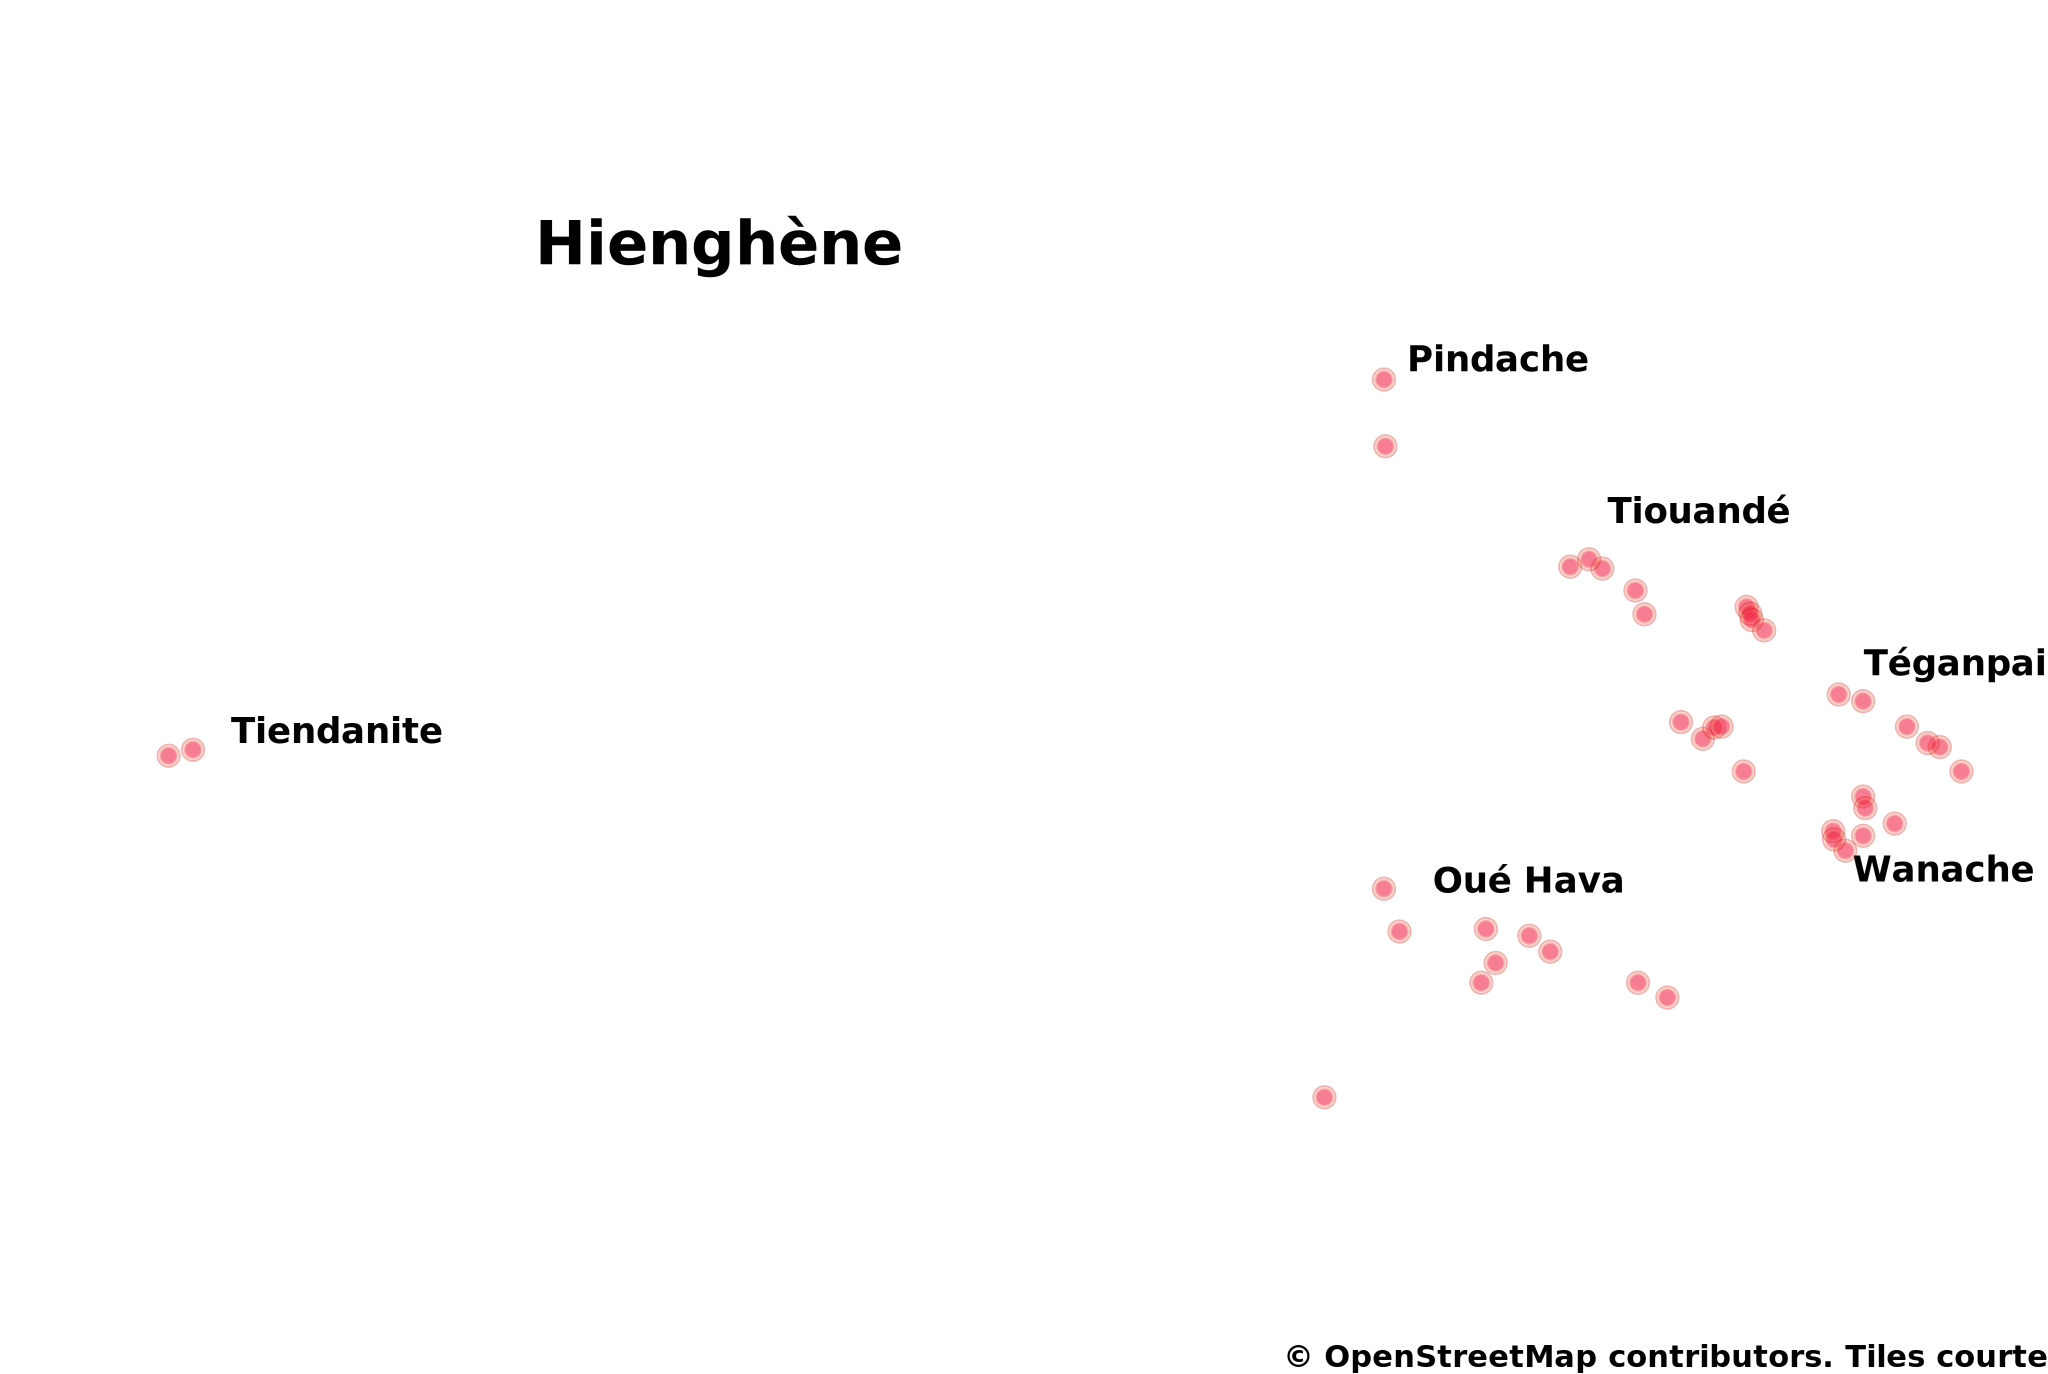
\includegraphics[width=\linewidth]{figures/map_dots.pdf}
	\caption{Map of speaker households. Approximate map of speaker households on the east coast (\citeauthor{gouvenementdelanouvelle-caledonie_explorateur_2019}, 2017-11-22), dots are my own, thanks to Florian Matter.}
	\label{map:dots}
\end{figure}

\subsection{Téganpaïk}
\ort{Téganpaïk}, or in Pije [tʰeᵑgane ˈpaːik] \qu{split stone}, after a placename close to the cemetery, is a village of about 200 inhabitants. Haudricourt translates the name as \textit{tnek-ngen-paik} \qu{oven-in-stone} \parencite[229]{haudricourt_langue_1968}.%The chieftaincy is held by a Oué man, but traditionally belongs to the Néa clan. 
A Shell gas station, a community center and a church are the only public buildings; the closest school is in Cèmuhî-speaking Touho, though many children go even further to Paicî-speaking Poindimié for secondary education. Téganpaïk is the biggest Vamale-speaking village, and the research project was based there. Traditionally Pije, many families are bilingual, and old marriage alliances have brought women speaking other languages as well. In most families, Kanak language transmission stopped around 1990. %almost all of my first, exploratory field trip there, with members of the Pei family.
The village is a string of houses along the national road RN1 and squeezed between steep mountains and the sea (there are rarely more than 100 metres between them). While the pre-contact population of the fertile Tipije (Pij. \textit{ti pije} \qu{estuary snare}, the Pije name for the river itself is \textit{le pije} \qu{in snare}), and Tiwaka valleys, was likely large, this coastal strip harbors no fields and few fruit trees, and may not have been as densely populated before the arrival of Vamale speakers. Almost beachless, and facing sharp, mostly dead coral at low tide, Téganpaïk does not attract many tourists, and with a chiefly ban on kava bars,\footnote{The next village to the East, \ort{Kongouma} (Cèm. /ko-goo-mwa/ \qu{on the wall}), sports three \textit{nakamals} and kava drinkers come from Hienghène and Touho to lift \textit{sels}.} the only points of interest to travelers are the Shell gas station and a picknick area near the sea. Touho has a diving school and boats one can rent, whereas the only bigger boat the village had, the \textit{Dongan}, was lifted and crashed on the other side of the road by cyclone Betty in 1995. This disbanded the fishing cooperative that had begun between villagers, and the boat's low-tide haven, a pool created by coral blocks, is now used for swimming and as a sardine reproduction sanctuary. Cyclones are becoming stronger almost every year, and with warmer, more acidic waters, the coral barriers protecting Grande Terre against the occasional tsunamis and other high waves are deteriorating. Villagers have begun planting mangrove trees to attract fish and crabs, but also as a protection against coastal erosion and waves. The author did not meet anybody unworried about climate change.

Téganpaïk is a tightly-knit community. Its children play together, the men go hunting on horseback and in pickup trucks and fish on bamboo rafts and in motorboats. The protestant church is an important center to the community, and one of the main domains of Vamale.
Téganpaïk's clan council also administrates Wanaa (see \sectref{subsec:Wanaa}) as well as the former leper colony Mahena/Ma\"ina, which is composed of few houses and can be considered a suburb of Téganpaïk.

\begin{figure}
	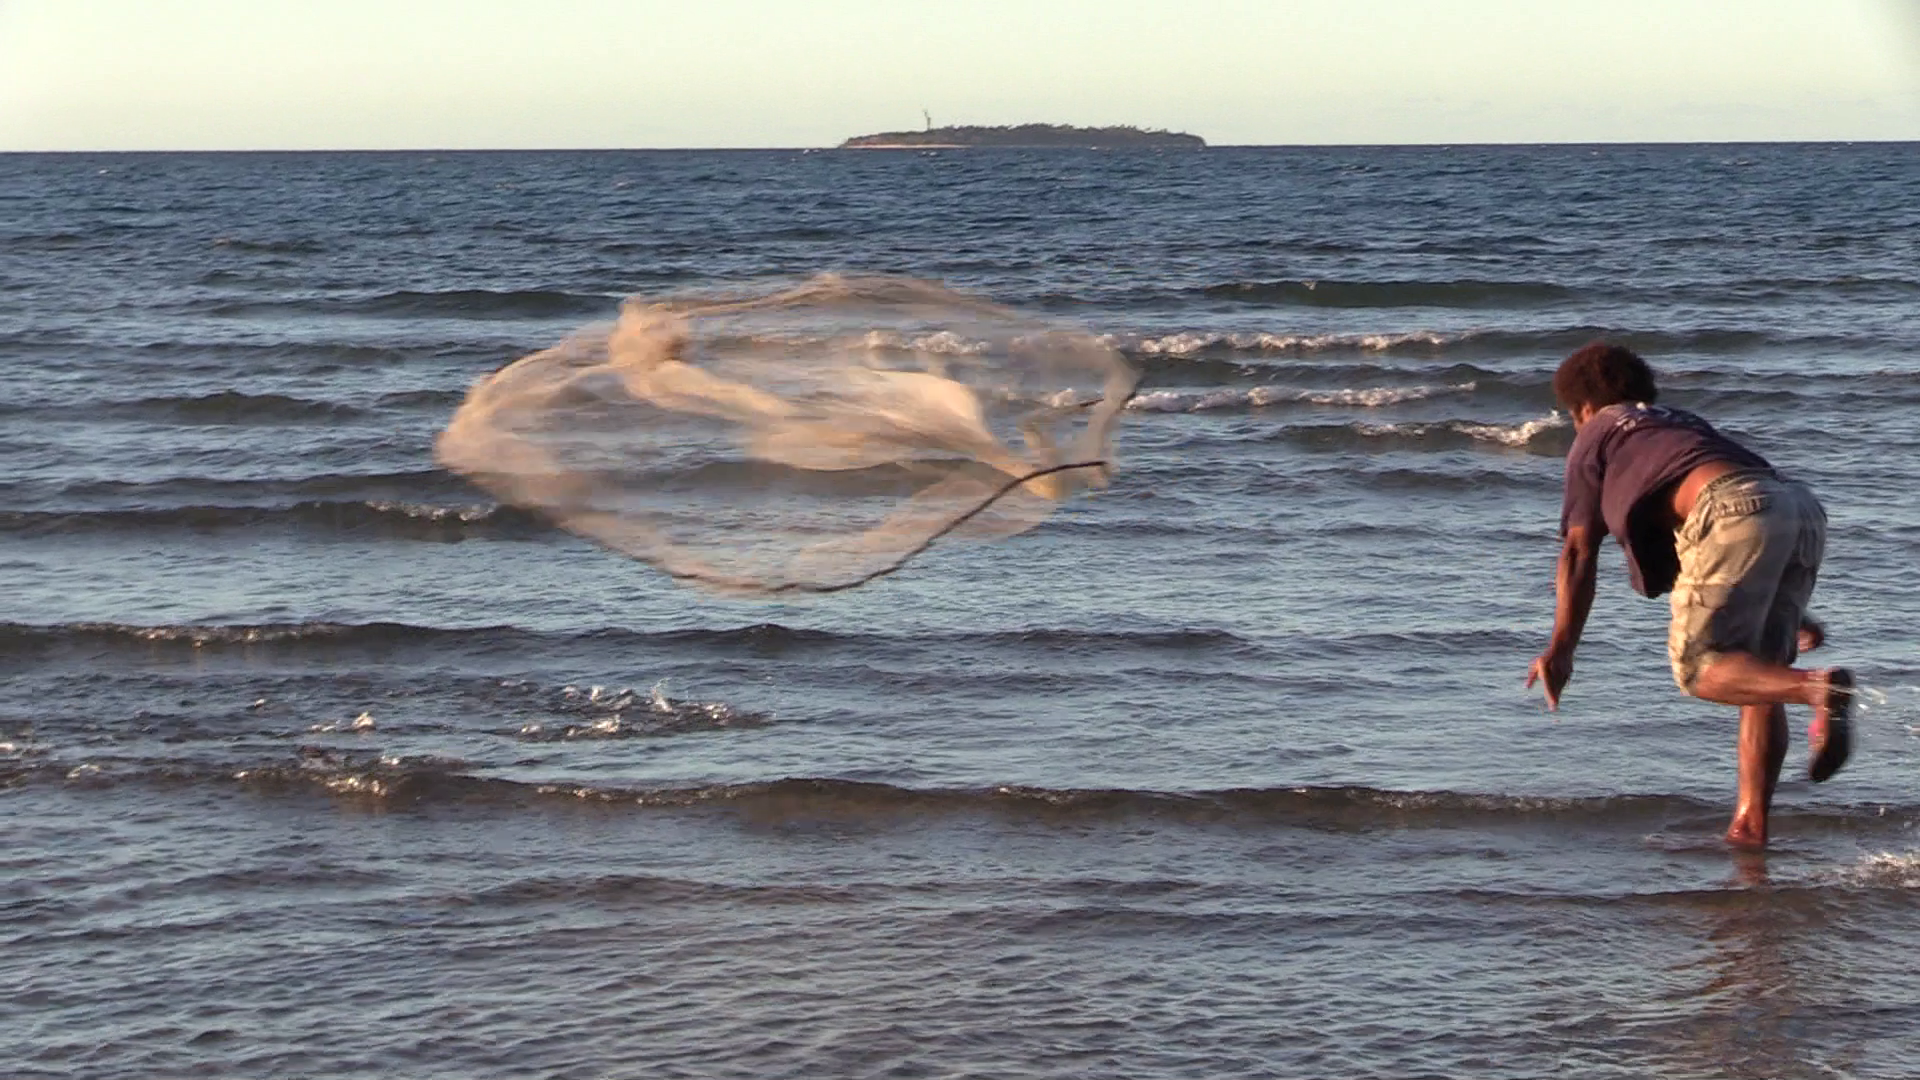
\includegraphics[width=\linewidth]{figures/net}
	\caption{Mr.\ Christophe Pei fishing for sardines in Téganpaïk}
\end{figure}

\subsection{Wanaa}
\label{subsec:Wanaa}
\ort{Ouanache} [wãˈnãː]\footnote{According to inhabitants, possibly from Pije \textit{hwada} \qu{planting spot} \parencite[106]{haudricourt_dictionnaire_1982} or Vamale \textit{(e-)wanaa} \qu{dispute}.} has only 11 houses, but fluent child speakers of Vamale, and many fields belonging to Téganpaïk inhabitants. %Dui's biological mother lives here.
Wanaa was Pije-speaking before 1917, but is now one of the biggest speaker-centers of Vamale. Contrary to Téganpaïk, it is an official tribe, though its chief Luc Oué resides in the former village. A war location in 1917, it welcomed some of the inland refugees.
The village concentrates in two road loops close to the neighboring villages Téganpaïk and Tiouandé, but the tribal grounds stretch south-east following a valley shown in \Cref{fig:wana} until a mountain pass leads to Poyes (see \chapref{chap:Tipije}).
Considering that some of its uninhabited mountain flanks show remains of taro terraces, and that planted araucaria trees can be seen much further upstream, the settling of youths in the wild backyard of the village, Tanaka, is more a reclaiming of former living grounds than a human invasion.

\begin{figure}
	\centering
	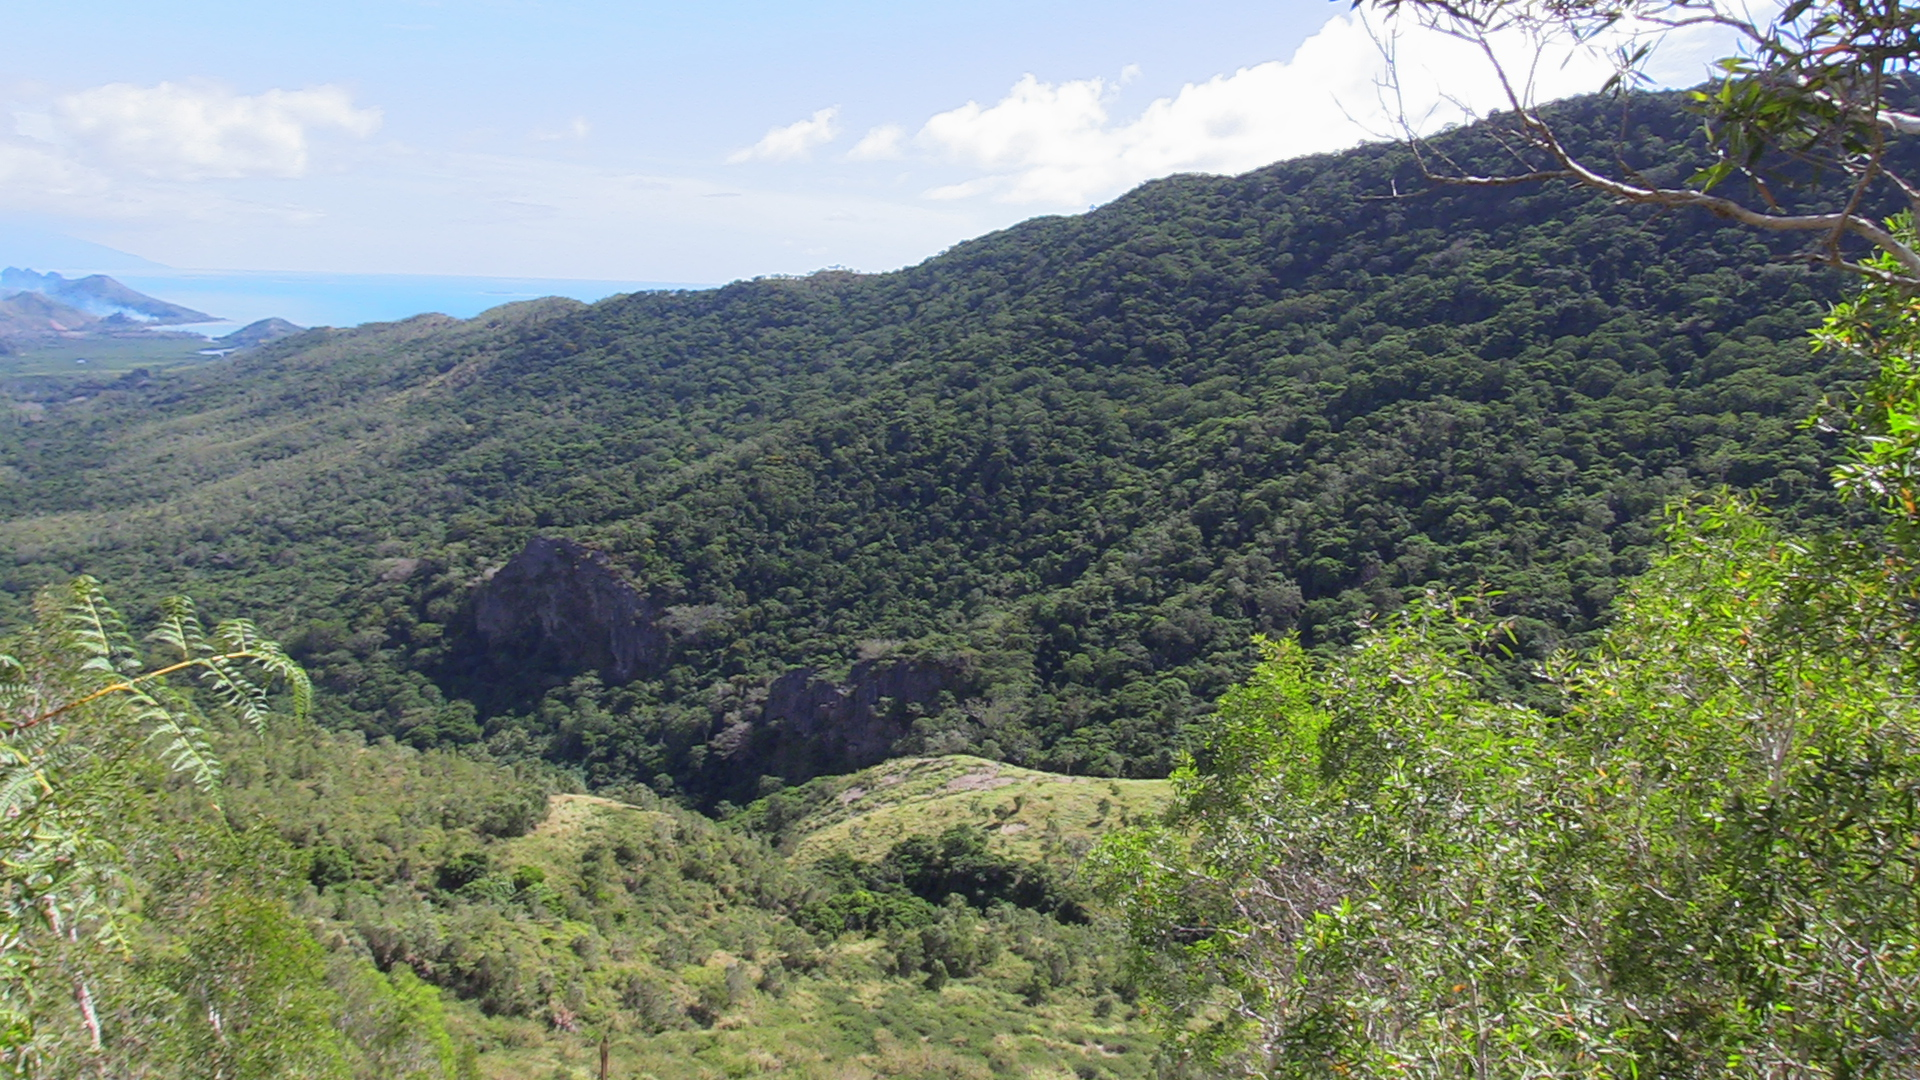
\includegraphics[width=\linewidth]{figures/wanaa}
	\caption{The Kacabwec valley leading to Wanaa. Only part of it is inhabited now.}
	\label{fig:wana}
\end{figure}

\subsubsection{Tiouandé}\largerpage[2.25]
\ort{Tiouandé} (Pije [tʰeˈxʷaːⁿde] \qu{rock garden}) borders the Tipije river on its northernmost end, the sea on the northeastern side, steep mountains and rock formations like ``Napoleon's hat" (Vam. \textit{vaci that} \qu{wind's nucleus}) on the west (shown on the left in \Cref{fig:twd}), and the hill Kapohiyoak (``children-making place") %suffering from deforestation-induced erosion 
which separates it from Téganpaïk. Tiouandé is the village with the most Pije speakers in the region, and is in close and active contact with Téganpaïk. Its chieftaincy is held by the Kalène clan, though the Bwiyâ have held it until the current chief took over. %\textit{fuâ bonu} \ort{Fouan Bonou} and her son \textit{nigai} (\ort{Ningaille}) live there.

\begin{figure}
	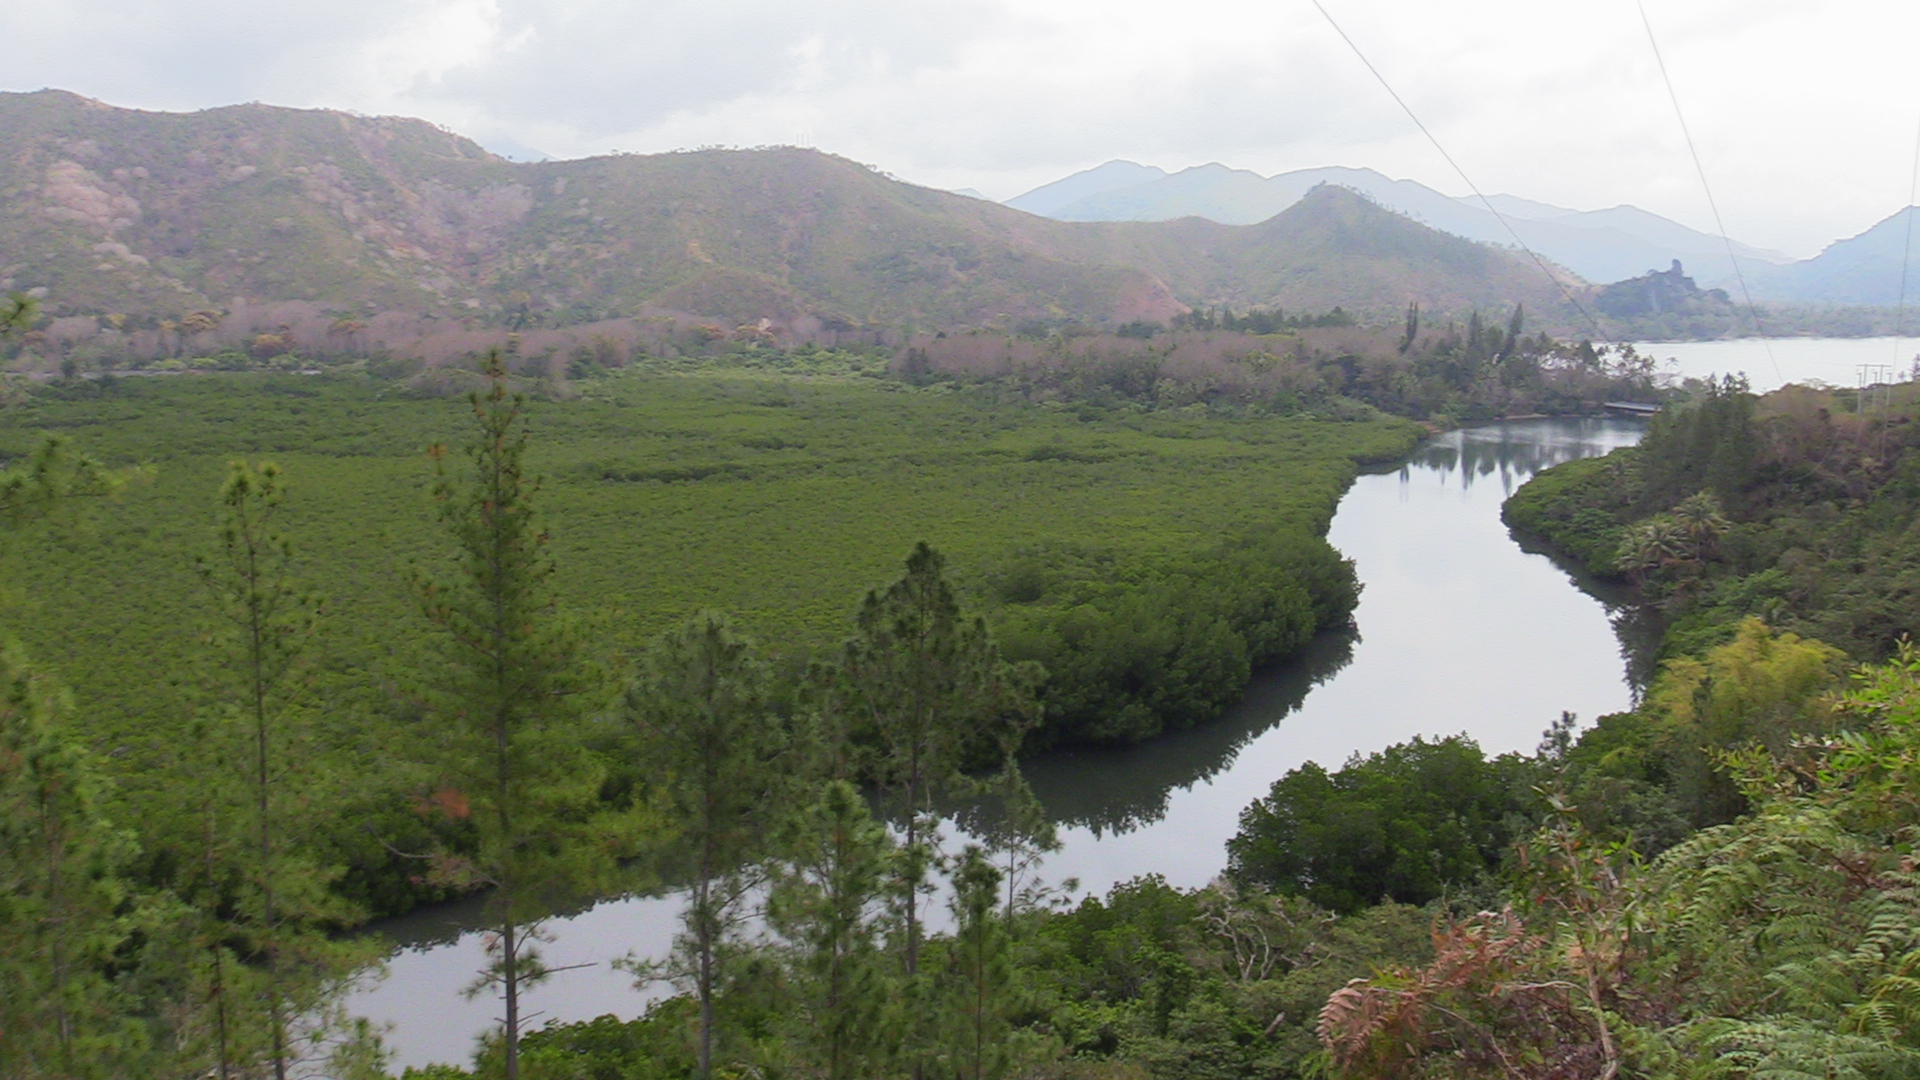
\includegraphics[width=\linewidth]{figures/twd}
	\caption{The Tiouandé estuary}
	\label{fig:twd}
\end{figure}

\subsection{We Hava}\largerpage[2]
\ort{Oué Hava}, Vam. ['we hava] \qu{\textit{Broussonetia papyrifera}\footnote{Used for its bark to make \textit{tapa} cloth.} creek}, %though some speakers mentioned \qu{ghost creek}, 
built along a tributary of the Tipije river, is a group of settlements, about four or five, each consisting of several huts and small houses. An exception makes a classic colonial building, white and facing the river, which is now inhabited by We Hava's former chief Kaina Fouan. The chieftaincy has returned to the traditional owners, the \ort{Tchéou} /ceu/ clan. The long road to \textit{Cake-O} \qu{scoop, bail out-bamboo}, We Hava's last dwelling and home of the oldest Vamale speaker Philippe Gohupe (the author of the Tipije text in \Cref{text:tipije}), is now bordered by bamboo groves and forest in various states,{\interfootnotelinepenalty=10000\footnote{Burning brush is a problem for local forestry. While careful burns were part of the slash-and-burn agricultural model, unsupervised fires are a common cause nowadays for wildfires, and are universally frowned upon and creates problems for wildlife, water table, and of course botany. The straw needed for traditional thatching is especially vulnerable.}} but all along the road, traces of abandoned villages can be seen on both sides of the river. We Hava and the settlement on the other side, Tipije, are what remains of ca. 14 settlements in the valley.

\begin{figure}
	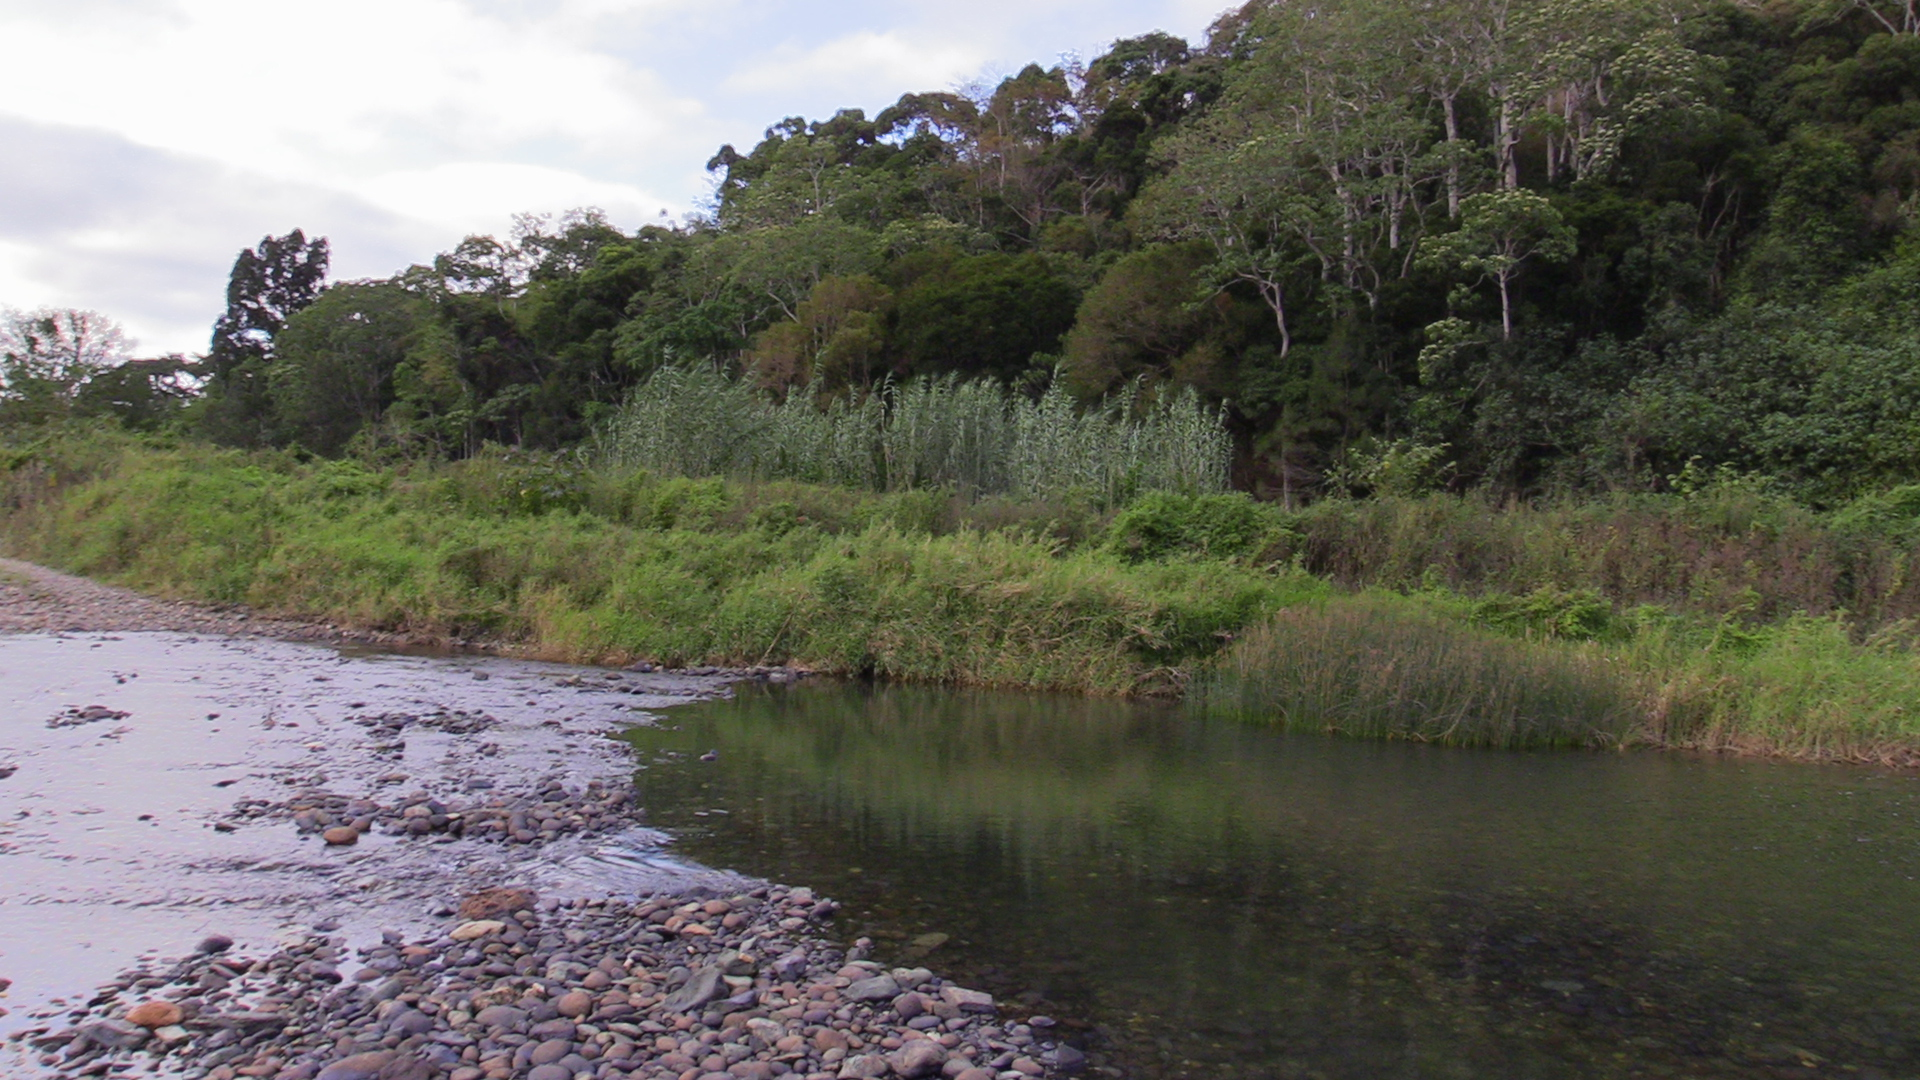
\includegraphics[width=\linewidth]{figures/wehava}
	\caption{The We Hava river}
\end{figure}

\subsection{Tiendanite}
\ort{Tiendanite}, in Vamale ['seːⁿɟan̥it], the home village of the politician Jean-Marie Tjibaou, is buried in misty hills up-stream of a Tipije tributary. It mostly houses eastern Nemi and Mountain Pije speakers, but also three households of Vamale Usa speakers, who are in irregular contact with coastal speakers. Usa is a Voh-Koné variety formerly spoken in a valley tributary to Pamale, and has a half-dozen speakers under 40 years of age. %The daughter is my age and speaks it. 
Children run around speaking Pije. Vamale speakers arrived there after the war \parencite[62]{couhia_pascal_2008}, though their earlier presence is likely. %A beautiful, remote place. 

Having provided a brief overview over the places in which Vamale is spoken, the chapter now introduces some important societal points.

\section{Language family}
\label{sec:Ling_Profile}
\largerpage
%This section is about the genealogical context of Vamale. 
\textcite[112]{lynch_oceanic_2002} classifies the New Caledonian language family and the Southern Vanuatu family as part of the Southern Melanesian family. With South Efate languages, this group forms the Southern Oceanic linkage \parencite[112]{lynch_oceanic_2002}, itself a linkage in East Malayo-Polynesian (see \Cref{fig:SouthOceanic} for a map). \textcite[334]{lynch_efate-erromango_2004} hypothesizes that New Caledonia was settled rather directly from Efate, which would make sense with its status of a family inside a linkage.
Oceanic languages are grouped into innovation-defined groups and innovation-linked ones \parencite[93]{lynch_oceanic_2002}, distinguishing languages which descend from a reconstructible proto-language, from languages that form a group through innovations shared via contact, or where innovations have occurred in overlapping smaller groups. The latter case is much more frequent in this area of the world. 
\begin{figure}
% 	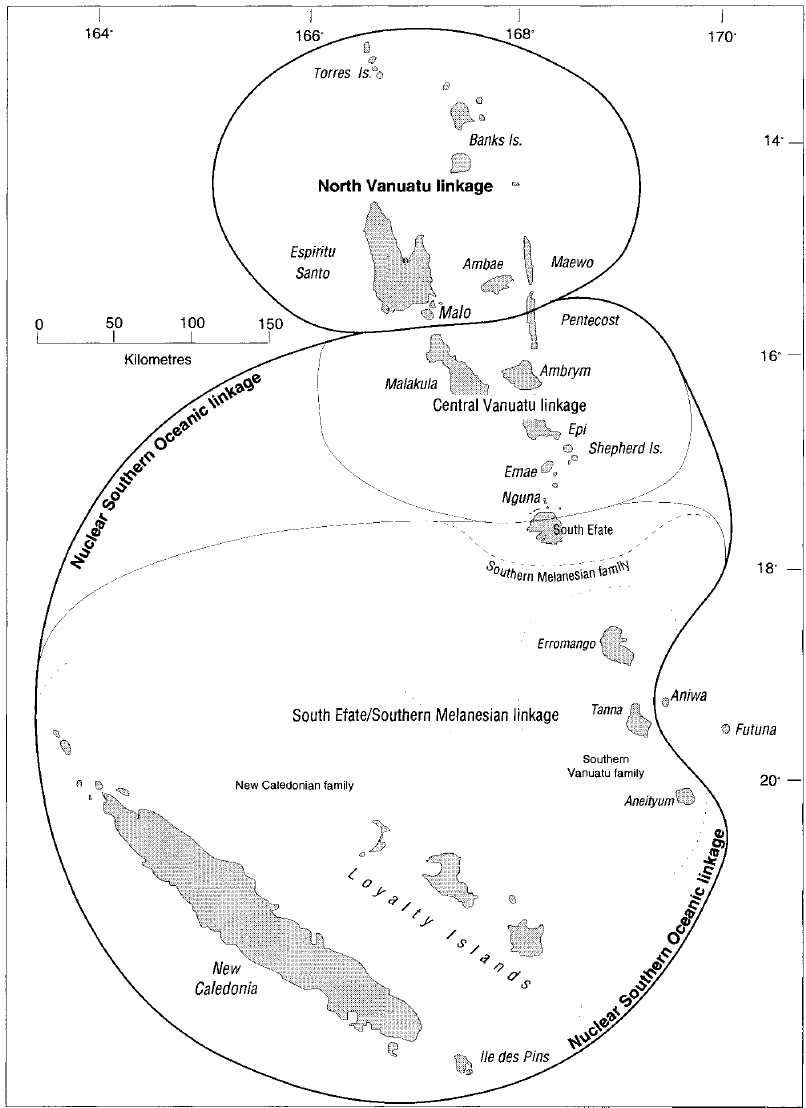
\includegraphics[width=\linewidth]{figures/lynch_south_oceanic}
	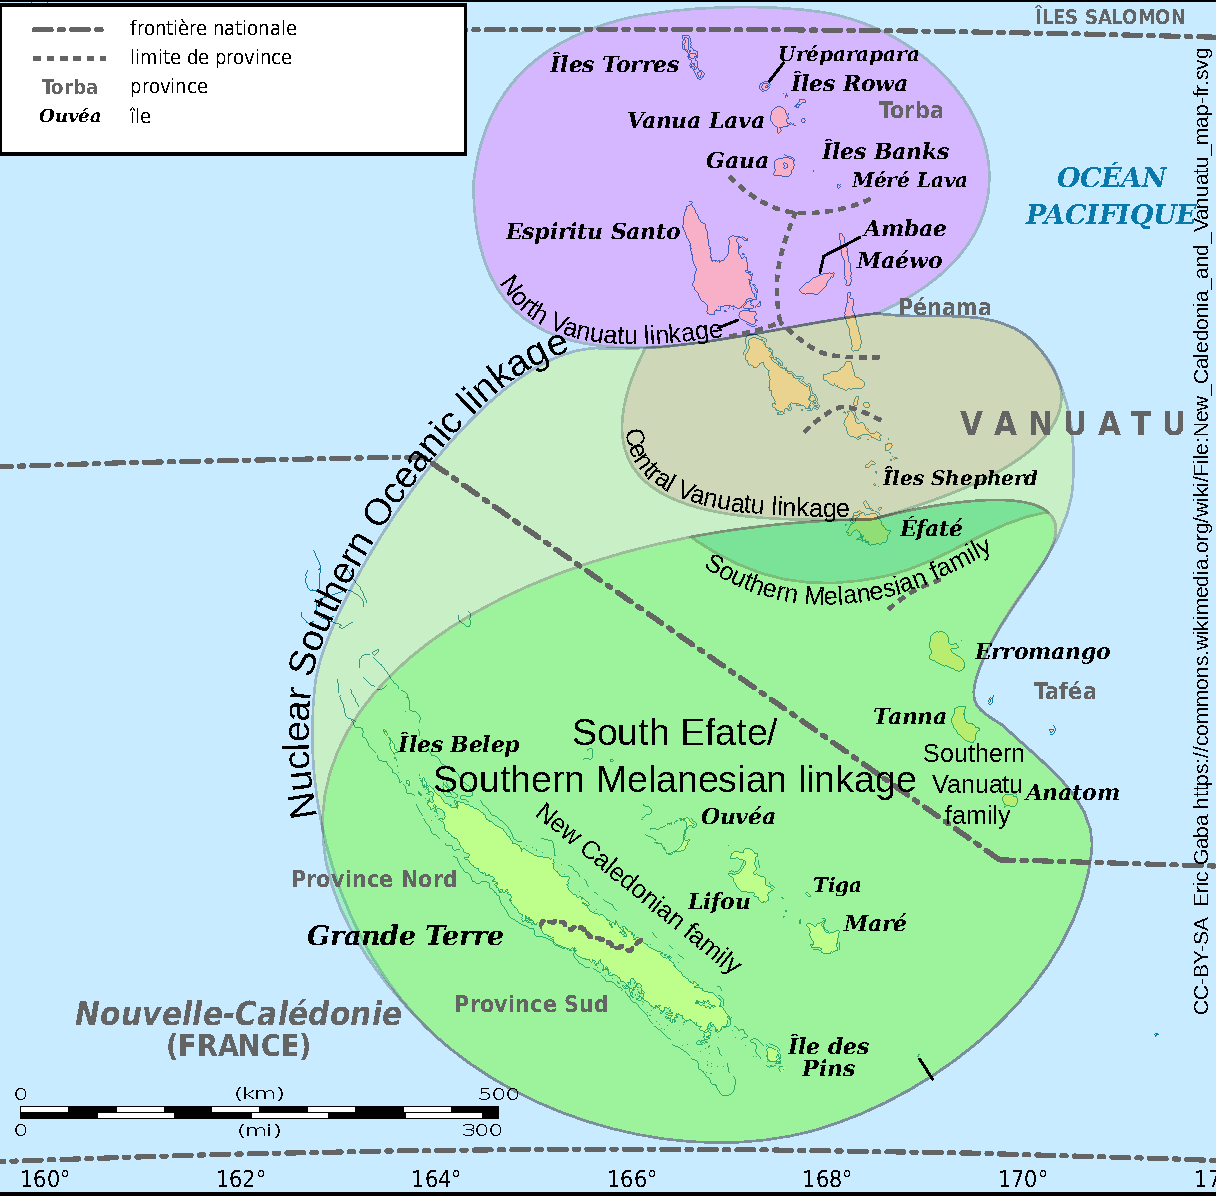
\includegraphics[width=\linewidth]{figures/lynchetal2022b.pdf}
	\caption{New Caledonian within the Southern Oceanic linkage \parencite[113]{lynch_oceanic_2002}}
	\label{fig:SouthOceanic}
\end{figure}
%\begin{table}
%	\caption{Proto-Oceanic consonantal phonemes, reproduced from \textcite[25]{ozanne-rivierre_phonologie_1982}}
%	\begin{tabular}{lccccccc}
%		& ``Labio-velar" &	Labial&	Dental&	Retroflex&	Palatal&	Velar&	Uvular\\
%		\multirow{3}{2cm}{Oral}&	&	*p&	*t&	*d&	*s/*ɟ&&\\
%		&&&&&&*k&*q\\
%		& *w&&*l&&*j&*R [ɣ]&	\\
%		Semi-nasal&	*ŋp/mp&	*mp&	*nt			&&*ns&*nk&\\	
%		Nasal&	*ŋm/m	&*m	&*n	&&	*ɲ&	*ŋ&	\\
%	\end{tabular}
%	\label{tab:POC_phon}
%\end{table}

Lynch uses the term ``Southern Oceanic" to refer to \qu*{a linkage whose members today comprise the 130 or so non-Polynesian languages of Vanuatu and New Caledonia} \parencites{lynch_southern_1999}[313]{lynch_efate-erromango_2004}. The linkage is defined by the innovations from Proto-Oceanic (POc) listed below, among others. 
\begin{itemize}
\item POc *R was dropped in absolute word-final position \parencite[313]{lynch_efate-erromango_2004} %, and t nonfinally in at least eight particular lexical items, though it was retained in most other etyma in nonfinal position." 
While northern New Caledonian languages do not feature \textit{-l} or \textit{-r} in non-loans, possessed forms hint at a merger with \textit{-t} rather than an apocope; compare Vamale \textit{fedat} \qu{blood} from POc *daaR to its possessed form \mbox{\textit{fedala-}.}
%[\ldots] A number of forms containing a bilabial in an earlier protolanguage replaced this with a labiovelar in PSO (see Lynch 2002). 
\item ``Third person pronouns accreted *na-." \parencite[313]{lynch_efate-erromango_2004} The singular article *na- was not conserved in New Caledonian, but \textcite[197--201]{ozanne-rivierre_proto-oceanic_1992} argues that a trace was responsible for some non-etymological prenasalized consonants \parencite[316]{lynch_efate-erromango_2004}. Compare *talik \qu{sea} $\rightarrow$ Vamale \textit{ⁿjati}. 
\item ``POc *k $\rightarrow$ Proto-Southern Oceanic (PSO) *g in some pronouns" \parencite[316]{lynch_efate-erromango_2004}. Compare \begin{itemize}
\item *POc *kita \qu{1\gl{pl}.\gl{incl}} $\rightarrow$ Southern Melanesian *gida or *gadV $\rightarrow$ Vam. \textit{gase}
\item  *POc *ko \qu{2\gl{sg}} $\rightarrow$ PNC, and Vam. \textit{go}
\item *POc *ka[m]u, *kamiu \qu{2\gl{nsg}} $\rightarrow$ PNC *ga(m)u $\rightarrow$ Vam. \textit{gau} \qu{2\gl{du}}
\end{itemize}
\item ``The ancestral system of two transitive suffixes reduced to one (or none)." \parencite[313]{lynch_efate-erromango_2004}. This relates to the transitive suffixes *-akini and *-i, both of which may still have reflexes in Vamale in the form of \textit{-ke} and \textit{-i}, respectively (see \sectref{ssec:ke_i}). While \textit{-i} is found in many northern languages, \textit{-ke} may now be unique to Voh-Koné. This potential disagreement with Lynch is grounds for more research.
%* A locative preposition PSO *(a,i)lo developed from the POc noun *lalo- 'inside'. 
%* POc *mataqu 'right (hand/side)' underwent metathesis as PSO *matuqa (see 2.3.4 below). There are some irregular developments in other lexical items, as well as some apparent lexical innovations." 
\end{itemize}
\largerpage

Southern Oceanic contains the Southern Melanesian family, defined amongst other things by its voicing of the initial plosive in certain pronouns (e.g. POc *kita \qu{1\gl{incl}} $\rightarrow$ SM *gida, later *gadV $\rightarrow$ Vam. \textit{gase}\slash\textit{gasu}) \parencite[317]{lynch_efate-erromango_2004}. New Caledonian as a family is well-defined by sound changes, listed below, and some lexical innovations \parencite[316]{lynch_efate-erromango_2004}. \Cref{tab:PNC-VK} summarizes and illustrates some of the consonant sound changes from Proto-Oceanic through Proto-New Caledonian, to modern-day Vamale and Bwatoo.

\begin{itemize}
	\item Merger of POc *c, *s $\rightarrow$ *s
	\item Merger of POc *n, *ñ, *l $\rightarrow$ *n
	\item Loss of POc *R and *y
	\item POc *puV  $\rightarrow$ PNC *pʷV
	\item POc *ai $\rightarrow$ PNC *e\slash *eː \parencite[317]{lynch_efate-erromango_2004}
\end{itemize}
\vskip-\baselineskip
\largerpage[2.5]
\begin{longtable}{llll}
	\caption{Voh-Koné reflexes of POc forms\label{tab:PNC-VK}}\\
	\lsptoprule
	\multicolumn{2}{l}{POc form} &  Bwatoo & Vamale\\\midrule\endfirsthead
	\midrule
	\multicolumn{2}{l}{POc form} &  Bwatoo & Vamale\\\midrule\endhead
	\endfoot\lspbottomrule\endlastfoot
	\multicolumn{2}{l}{Proto-Oceanic} & \\
	& *p &&\\
	\multicolumn{2}{l}{PNC} & \\
	& *p, *pw $\rightarrow$ v, vʷ	&&\\
	& *paRi \qu{ray(fish)}&\textit{ve}& \textit{ve}\\
	%	*pulu	\qu{hair}&	\textit{vuu}-	&	\textit{vuu}-\\
	& *poñu	\qu{turtle}&	\textit{vʷen}	&	\textit{vʷen}\\
	\multicolumn{2}{l}{PNC} & \\
	& *pp, *ppw	$\rightarrow$ f, fʷ&&			\\
	& *posi	\qu{press}&	\textit{fʷati}	&	\textit{fʷati}\\
	\multicolumn{2}{l}{POc} & \\
    & *d / *r&&\\
	\multicolumn{2}{l}{PNC} & \\
    & *t, *nd $\rightarrow$ ⁿd&&\\			
	& *daun	\qu{leaf}&	\textit{ⁿdoon}	&	\textit{ⁿdoon}\\
	& *daRoq	\qu{ground}&	\textit{ⁿdoot}	&	\textit{ⁿdoop}\\
	\multicolumn{2}{l}{Proto-North} & \\
	& *tʰ&&		\\
	& tʰat	\qu{pandanus}&	\textit{tʰat}&		\textit{tʰat}\\
	& tʰap	\qu{oral thrush}&	\textit{tʰap}&	\textit{tʰap}	\\
	%tʰoo	&	& tʰoo	&&	\\
	\midrule
	\multicolumn{2}{l}{POc} & \\
	& *t&&\\
	\multicolumn{2}{l}{PNC} & \\
	& *t̪, *d̪ $\rightarrow$ ⁿɟ&&\\
	& *tasi	\qu{younger sibling}&\textit{ⁿɟati}- &	\textit{ⁿɟati}-\\
	%& (same gender)&&&\\
	& *tupa	\qu{grandfather}&\textit{ⁿɟiᵐbu}-ⁿɟiᵐbu-\\
	\multicolumn{2}{l}{PNC} &\\
	 & *tt $\rightarrow$ θ/s&&\\			
	%	*tuka	\qu{elder}&	\textit{θia}-& \textit{sia}\\
	& *tumpuq	 \qu{swollen}&\textit{θiᵐbu} &	\textit{siᵐbu}\\
	\midrule
	\multicolumn{2}{l}{POc} & \\
	& *s&&\\
	\multicolumn{2}{l}{PNC} & \\
	& *s, *ⁿs $\rightarrow$ d/t&&\\
	%*sai&	who?	& ⁿde&	kai\\
	& *sapa	\qu{what?}&	\textit{ⁿda}&	\textit{ⁿda}\\
	& *sake	\qu{go up}	& \textit{ta}	&	\textit{ta}\\
	& *suRi	\qu{bone}&	\textit{ⁿduu}-	&	\textit{ⁿduu}-\\
	\multicolumn{2}{l}{PNC} & \\
    & *ss $\rightarrow$ tʰ&&			\\
	& *susu	\qu{breast}&	\textit{tʰi}	&	\textit{tʰi}\\
	& *suki	\qu{pierce} &	\textit{tʰi}&		\textit{tʰi}\\ % <<<--- Enlarge 2nd Table Page.
	\midrule
	\multicolumn{2}{l}{POc} & \\
	 & *k&&\\
	\multicolumn{2}{l}{PNC} & \\
	& *k $\rightarrow$ ð/j \goodtilde ∅ &&\\			
	& *kulit	\qu{skin}&\textit{ðii}&\textit{i-}\\
	%*kuluR&&&&\\
	%	*kutu	\qu{lie (parasite)}&	\textit{ði}&\textit{i}\\
	& *kuRita \qu{squid}&\textit{ðiia}&\textit{iᵐbwen}\\
	\multicolumn{2}{l}{PNC} & \\
	& *kk $\rightarrow$ θ/s&&\\			
	& *kuku	\qu{claw}&	\textit{θi}-	&	\textit{si}-\\
	& *kau	\qu{swim}&	\textit{θoom}&		\textit{soom}\\
	\midrule
	\multicolumn{2}{l}{POc} & \\
	 & *q &&\\
	\multicolumn{2}{l}{PNC} & \\
	& *q $\rightarrow$ ɣ/∅&&\\
	& *qusan	\qu{rain}&\textit{ɣuta/ wuta}& \textit{uta}\\
	& *qupi	\qu{yam}&\textit{ɣuu}	&	\textit{uvu}\\
	& *qata	\qu{man} &\textit{ɣau}&\textit{ɣaju}\\
	& *qaso	\qu{sun}	& \textit{ɣat}&	\textit{ɣat}\\
	\multicolumn{2}{l}{PNC} & \\
	& *qq $\rightarrow$ x&&\\				
	& *quma	\qu{grow, cultivate} &\textit{xuum}&\textit{xumi}	\\
	& *qulos	\qu{worm}& \textit{xun̥at}&\textit{xun̥at}\\
\end{longtable}


\begin{sloppypar}
The Southern Oceanic languages spoken in New Caledonia can be split roughly into two groups: Mainland (i.e. \textit{Grande Terre}) languages, and the three Loyalty Islands languages Iaai, Drehu, and Nengone \parencite{ozanne-rivierre_proto-oceanic_1992}. Mainland languages split into northern and southern languages (see \Cref{fig:Mainland}), with a tendency for northern languages to have 5 or so vowel phonemes and over 35 consonant ones, and an opposite trend for large vowel inventories and small consonant ones in the South \parencite[25]{ozanne-rivierre_phonologie_1982}. In the North, a Far Northern branch (\textit{Extrême Nord} in French) and a Northern branch split into some dozen languages (see \Cref{map:North} for a map). 
\end{sloppypar}\largerpage


\begin{figure}[H]
 		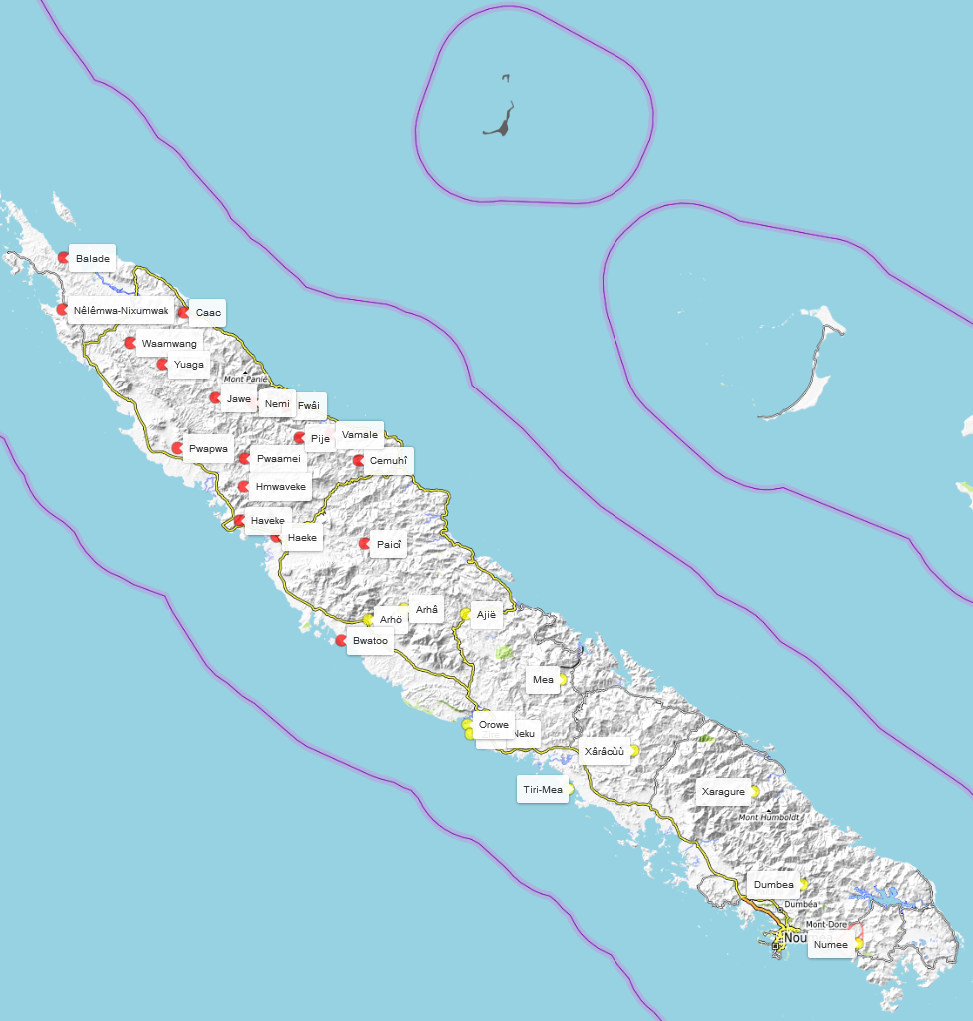
\includegraphics[width=\linewidth]{figures/Mainland_New_Caledonian}
		\caption{Mainland New Caledonian, North (red) and South (yellow) \parencite{hammarstrom_mainland_2020}}
 		\label{fig:Mainland}
\end{figure}


 %The Northern subgroup splits into three groups on the grounds of shared innovations: the small Extreme North group, the tonal Center group, and the North one, the latter of which includes Vamale's linkage Voh-Koné.
 The latter is split into the so-called Hienghène cluster, the Voh-Koné dialects, and the tonal languages Cèmuhî and Paicî, to which Voh-Koné is more closely related than to the other branches, \parencite[19]{rivierre_bwatoo_2006} see \Cref{fig:NorthTree} for a language tree. The language described in this book is part of the Voh-Koné cluster. The question of dialect vs language, as well as of the name given to the variety in question, will be addressed in \sectref{sec:LanguageName}.  

Voh-Koné is defined as a group mostly by phonological changes that set it apart from the rest of the Northern and Far Northern languages. Comparing sound changes in the Northern family is difficult due to sparse data. Valuable work was done by Haudricourt \parencite[73--97]{haudricourt_langues_1948} and especially Ozanne-Rivierre (\citeyear{ozanne-rivierre_structural_1995}, \citeyear{ozanne-rivierre_proto-oceanic_1992}). The following is mostly a summary of her work, with some Vamale data added. 

Compared to other Northern languages, Voh-Koné is mostly distinct by its lenition of *c $\rightarrow$ j and initial *p to v (see \Cref{fig:NorthTree}). The latter was dropped in some Vamale words such as the singular article *\textit{vi} $\rightarrow$ \textit{i} (but not the language's name). %Furthermore, Voh-Koné palatalized \textit{*t-} to /c/, a sound change the group shares with Jawe.
Geminates of *q, *k, *p, historically the result of reducing the first syllable in reduplicated contexts, yielded aspirated initial consonants everywhere in the North \parencite[57]{ozanne-rivierre_proto-oceanic_1992}, but have voiceless fricative reflexes in Voh-Koné (see \Cref{tab:PNC-VK}). Voh-Koné languages do have aspirated plosives which evolved from the same source, too, however. This is partly due to borrowing, but given their almost exclusive occurrence before nasal vowels, this study suggests that the leniting sound changes which led to a fricativization did not occur completely (see \sectref{ssec:Aspiration}).\largerpage


\begin{figure}[H]
	\begin{forest}
		for tree={
			forked edges,
			child anchor=west,
		    parent anchor=east,
		    grow=east,
		    anchor=west,
			align=center,
			inner sep=0pt,
		}[~
		[Extreme North]
		[Other Northern\\Languages
		[Nemi-Pije-Fwâi-Pwaamei-Pwapwâ \\{*mbw, mb ({/}\_o, u) $\rightarrow$ ŋgw}\\{*}mw $\rightarrow$ ŋgw
		[Nemi-Pije-Fwâi \\{*t $\rightarrow$ t, c ({/}\_i, e)}]
		[Pwaamei\\{*}t $\rightarrow$ c\\{*}c $\rightarrow$ y]
		[Pwapwâ\\{*}t $\rightarrow$ c]
		]
		[Jawe \\{*}t $\rightarrow$ c]
		[Voh-Koné-Cèmuhî-Paicî\\{*}c $\rightarrow$ y \\{*}t $\rightarrow$ c
		[Voh-Koné \\{*}p $\rightarrow$ v]
		[Cèmuhî-Paicî\\{*}CʰV $\rightarrow$ CV́]
		]
		]
		]
	\end{forest}
	\caption{Language tree of some North New Caledonian languages \parencite[63]{ozanne-rivierre_structural_1995}}
	\label{fig:NorthTree}
\end{figure}


 %  Another view, based on sound changes, places the Center group within the Northern languages, as represented in \Cref{fig:NorthTree} (\todo{whose view?}).%\begin{figure}
\begin{forest}
for tree={
%fit=band,
    child anchor=west,
    parent anchor=east,
    grow=east,
    draw,
    anchor=west,
  align=center,inner sep=0pt,
  {},
  }
[Northern 
  [
	[Extreme North
  [Caac]
  [Nêlêmwa-Nixumwak
  [Nêlêmwa]
  [Nixumwak]
  ]
  	]
  [Nyelayu]
  [Yuanga]
  ]
  [North (Proper)
	[Hienghène Languages
		[Nemi-Pije-Fwâi]
		[Pwaamei]
		[Pwapwâ]
	]
		[Jawe]
		[Voh-Koné-Cèmuhî-Paicî
			[Voh-Koné
				[Vamale]
					[Usa]
				[Hmwaveke]
				[Haveke]
				[Haeke]
				[Bwatoo]
			]
			[Cèmuhî-Paicî]
		]
	]
]
\end{forest}
\label{fig:NorthTree}
\caption{Language Tree of the North New Caledonian languages (\cite{ozanne-rivierre_structural_1995}:63 and )}
\end{figure}

Vamale is a member of the Voh-Koné languages, a group of mutually mostly intelligible varieties which forms a belt on the western shore from Voh to Népou including Koné and Baco, then follows the Tiéta river upstream and breaks off around Temala, before picking up again in the east around Tiendanite, Ouen Kout and We Hava (see \Cref{map:North}). As is typical of dialect chains, the varieties furthest apart have distinct grammatical morphemes, distinct lexicon, and different phonological systems. Because of this, Vamale and Bwatoo are not readily understood by speakers of the other variety. \Cref{tab:LeenhardtPN} compares Voh-Koné pronouns, along with Pwapwâ, a neighbor of Bwatoo, as they were recorded in the 1940s.  %The Voh-Koné languages form the Northern group of New Caledonian with the Hienghène languages, Pwapwâ, and Pwaamei, and the Central subgroup of tonal Cèmuhî and Paicî,  See \Cref{fig:NorthTree} for an illustration.
 
\begin{figure}
	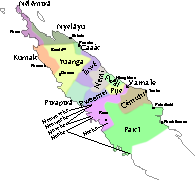
\includegraphics[width=\linewidth]{figures/north_new_caledonia2.pdf}
	\caption{Northern New Caledonian languages \parencite[45]{ozanne-rivierre_structural_1995}}
	\label{map:North}
\end{figure}

\begin{sidewaystable}
	\caption{Voh-Koné object-indexing pronouns after \textcite[504--507]{leenhardt_langues_1946}, modern Vamale added on the left.}
	\begin{tabular}{lllllllll}%{p{1.6cm}|p{1cm} p{1cm}lllll|l}
	\lsptoprule
		& \multicolumn{2}{c}{Vamale}&	Hmwaveke&	Waamwang&Haveke&	Haeke&	Bwatoo &Pwapwâ\\\cmidrule(lr){2-3}
		&   now   & 1946 & \\\midrule
		1\textsc{sg}	&\textit{ (e)o}&	\textit{o}&	\textit{yo}&	\textit{ng}&	\textit{ng}&	\textit{ong/ ng}&	\textit{ng}&\textit{ng}\\
		2\textsc{sg}&	\textit{ko}&	\textit{ko}&	\textit{go}&	\textit{m}&	\textit{go}&	\textit{go/ m}&	\textit{m}&\textit{m}\\
		3\textsc{sg}&\textit{(e)a}&	\textit{kon, ke}\footnote{Note that \textit{kon} may refer to an oblique marker \textit{ko-n} and \textit{-ke} is a transitive suffix.}&	\textit{kon, ke}&	\textit{n}&	\textit{gon}&	\textit{mon/ n}&	\textit{n}&\textit{n}\\
		1\textsc{du}.\textsc{incl}&	\textit{ju}&	&&&	&&					\textit{ju}&\\
		1\textsc{du}.\textsc{excl}&	\textit{bu}&			&&&&&				\textit{bu}&\\
		2\textsc{du}&	\textit{u}	&			&&&&&			\textit{u}&\\
		3\textsc{du}&	\textit{lu}	&					&&&&&	\textit{lu}&\\
		1\textsc{pl}.\textsc{incl}&	\textit{ga}&	\textit{ga}&	\textit{ga}&	\textit{je?}&	\textit{gaie}&	\textit{ngaie/ je}&	\textit{je}&\textit{je}\\
		1\textsc{pl}.\textsc{excl}&	\textit{be}&	\textit{be}&	\textit{be}&	\textit{be}&	\textit{gabe}&	\textit{ngabe/ be}&	\textit{be}&\textit{be}\\
		2\textsc{pl}&	\textit{gavʷe}&	\textit{gae}&	\textit{vʷe}&	\textit{we}&		\textit{gae}& \textit{o}&	\textit{e}&\textit{e}\\
		3\textsc{pl}&	\textit{le}&	\textit{le}, \textit{ke}&	\textit{le}&	\textit{le}&	\textit{le, ke}&	\textit{le, ke/ le}&	\textit{le}&\textit{le}\\
	\lspbottomrule
	\end{tabular}
	\label{tab:LeenhardtPN}
\end{sidewaystable}
%The possible closer relationship between Jawe and Voh-Koné languages has not yet been studied in detail, but may be of interest. Jawe, like Vamale and other Voh-Koné languages, has seen the (typologically unremarkable) sound change *t $\rightarrow$ c, as have the Hienghène languages. However, Pije and Nemi have conserved the old post-nasalised consonants k\textsuperscript{n}, t\textsuperscript{n}, which in Jawe and Voh-Koné gives k\textsuperscript{h}Ṽ, k\textsuperscript{h}Ṽ, with the postnasalisation expressed on the vowel (eg. \textit{kniik} $\rightarrow$ \textit{khîî} \qu{swamp fowl}), see \Cref{ssec:Aspiration}. On the other hand, \Cref{map:languages_1917}, showing the situation in 1917, places a contiguous Nemi-speaking land between the Jawe and Vamale areas. Jawe may have simply evolved alongside Voh-Koné and Cèmuhî-Paicî before the current geographical situation was set.

The languages of Voh-Koné probably spread from the eponymous region on the west coast to the Upper Tiéta valley, where Hmwaeke\footnote{\textit{hmwaeke} is a common greeting in the eponymous variety meaning \qu{how [is it going]?}.} is spoken. Until the early 20\textsuperscript{th} century, the neighboring valleys of the Pamale and its tributaries were inhabited by some 2,000 people according to oral tradition \parencite[62]{couhia_pascal_2008}. Since this region fell under colonial control only in the wake of World War I, no census before the Tipije war can confirm or contest this number. The entire population of the valley was either killed or scattered (see \chapref{chap:Tipije}). A map of the main movements can be found in \Cref{map:fugitives}. Those who went west assimilated into their linguistic cousins, whereas the eastward fugitives kept a language alive which they call Vamale today. Leenhardt called it \qu{'Moaeke} of the East Coast and counted 50 speakers \parencite[162]{leenhardt_langues_1946}.

%the kon/ke thing might be xale koon, xaleke X?
%\todo{include? cuz looks like OBJ paradigm}

%\subsection{Phonological clues}

%POc *q $\rightarrow$ Proto-New Caledonian, changed to voiced fricatives in Voh-Koné, where other North New Caledonian languages kept \textit{k} \parencite[57]{ozanne-rivierre_structural_1995}. The geminate *qq became *kh in Proto-North, and a palatal \textit{c} in modern languages

%POc  developed stops \parencite[200]{ozanne-rivierre_proto-oceanic_1992}. 

%The POc tap consonant *d / *r as well as the fricative *s changed to plosives, e.g. *\textit{sake} $\rightarrow$ \textit{ta} \qu{go up} \parencite[19]{rivierre_bwatoo_2006}.
\begin{sloppypar}
Within Voh-Koné, the major division opposes western, coastal varieties and eastern, mountain-based ones.
Interdental fricatives /θ/ and /ð/ are features of Bwatoo, Haveke, Haeke and Waamwang, whereas Hmwaveke and Vamale present the alveolar fricative /s/ instead of /θ/, and have lenited /ð/ to /j/, or dropped it before /i/ (e.g. *kulit \qu{skin} $\rightarrow$ Bw. \textit{ðii}, Vam. \textit{i-}).
\end{sloppypar}

Proto-Oceanic initial *q has become /ɣ/ in Vamale, except before /u/ (e.g. *\textit{qusan} \qu{rain} $\rightarrow$ \textit{uta}); western varieties keep /ɣ/ before /u/. The only case of a voiced fricative before /u/ is an allophone of /h/.
[ɣ] is also dropped before /o/ (Bwatoo \textit{ɣop} \qu{high tide}, \textit{op} in Vamale).

Intervocalic /v/ within a morpheme is rare, which is a contrast to the western languages.\footnote{Except for \textit{fava} \qu{4}, but Pije \textit{hovac}, Fwâi \textit{fovec} \parencite[261]{haudricourt_dictionnaire_1982}. Bwatoo \textit{fae}, Oundjo-Haveke \textit{favac} \parencite[135]{rivierre_bwatoo_2006}.} Hmwaveke, part of the mountain group, still shows intervocalic /v/ lost in Vamale, which suggests that this sound change originated in the East. Finally, %most Voh-Koné languages kept /p/ in places where Vamale now has /v/ (e.g. \textit{vamale}), and 
some final consonants (chiefly /k/ and /c/) were lost in Vamale that remain in Hmwaveke.

Historical sources suggest %In conclusion, there are western, coastal varieties which probably form 
a sort of \textit{Urheimat}, given that Guiart mentions a bigger Haekic coalition on the west coast before the Paicî influx of the 18th and 19th centuries \parencite[131,260]{guiart_chefferie_1963}. Compare the map by Leenhardt in \Cref{map:languages_1917} to \Cref{map:North}: Voh-Koné languages retreated to the North, and the coast between Koné and Poya is almost exclusively Paicî-speaking today. Interestingly, the map treats Pwapwâ and Pwaamei as dialects of Nemi. As the map, along with many of the language materials in the book was compiled using second-hand accounts \parencite[xi,xiii,xlviii]{leenhardt_langues_1946}, its accuracy depends on the area depicted. Since Leenhardt himself traveled to Pamalé in 1903 \parencite{leenhardt_figures_1978}, we can rely on the map for Vamale's historical position, even if it was inaccurate by the time of its publication. Until 1917, Vamale was spoken in an area inhabited since 420–610 AD \parencite[172]{sand_certainly_2012} (though probably not by Voh-Koné speaking people), and represents the easternmost point of a putative inward expansion of a dialect continuum. 

Spatial proximity %close contact of the languages 
groups coastal Haveke and mountainous Hmwaveke together, so that there is a middle zone, as is typical of dialect chains. In addition to this blurring factor, language contact changed dramatically in the last century, with an influx of refugee Hmwaeke and Vamale speakers that changed Haveke and Hmwaveke. Vamale itself may have changed faster in its relative isolation.

\begin{figure}
	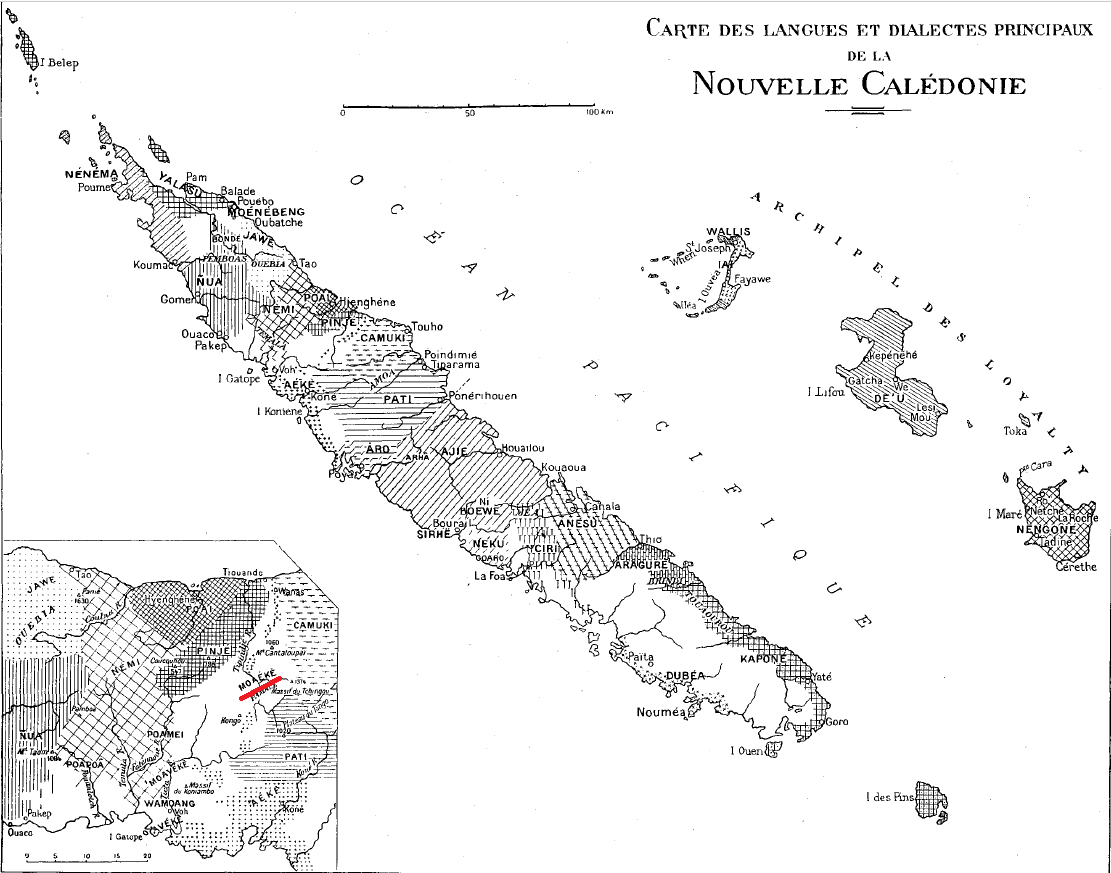
\includegraphics[width=\linewidth]{figures/leenhardt_map658}
	\caption{Languages in the region around 1917 \parencite[658]{leenhardt_langues_1946}, with Vamale (``Moaéké") underlined in red.}
	\label{map:languages_1917}
\end{figure}
%\begin{table}
%	\caption{Some isoglosses within Voh-Koné}
%	\begin{tabular}{cccccc}
%								& Vamale&					Hmwaveke&	Haveke&	Haeke&Bwatoo\\
%		\hline&&&&&\\
%		Intervocalic v&		No\footnotemark &	Yes &Yes& No&No\\
%		Initial ɣ-& No & No & Yes & Yes & Yes\\
%		Interdental fricatives & No & No & Yes & Yes & Yes\\
%		-p&						Yes& 							Yes&Yes	&Yes&-t\\
%	\end{tabular}
%	\label{tab:VK_inner}
%\end{table}
%\footnotetext{Except for \textit{fava} \qu{4}, but Pije \textit{hovac}, Fwâi \textit{fovec} \parencite[261]{haudricourt_dictionnaire_1982}. Bwatoo \textit{fae}, Oundjo-Haveke \textit{favac} \parencite[135]{rivierre_bwatoo_2006}}
 
 \begin{figure}
	\fittable{%
 	\begin{forest}
		forked edges,
		for tree={align=center,grow=south}
		[Voh-Koné
		[Coast
		[Haake\\Bwatoo]
		[(Waamwang)]
		[Haeke]
		[Haveeke]
		]
		[Mountain
		[West
		[Hmwaveke]
		[Hmwaeke]]
		[East
		[Usa]
		[Vamale]
		]]
		]
	\end{forest}}
 	\caption{Possible language tree of Voh-Koné languages}
 	\label{fig:VKTree}
 \end{figure}
 
 \subsection{Linguistic context}
 This section aims to describe how Vamale relates to other languages surrounding it.
 Historically, it is likely that the Voh-Koné languages spread eastwards into the mountains, which would suggest that Vamale/Hmwaeke is most closely related to Hmwaeke proper, then Hmwaveke, maybe Waamwang, and finally Haveke, Haeke, and Bwatoo.
 
 \is{Language contact}
 People formerly would cross the mountains on foot- and horse trails, leading to Pije, Fwâi, and Cèmuhî speaking areas, but more importantly other Voh-Koné speaking areas: Tiéta (Haveke), Temala (Hmwaveke), and some isolated houses in the middle, as well as diasporically in Bopope and Atéou. Nowadays, work in the nickel mines and the cargo ports, coupled with a lack of legal restrictions to buy cars without a driver's license, %and occasionally growing and selling cannabis 
 have afforded most families with the means of traveling long distances to visit relatives and maintain social ties. This, however, has also changed the languages with which Vamale speakers are in contact. Nowadays, cars dominate mobility and define it. Roads lead to Hienghène and Touho, so Fwâi and Cèmuhî have gained influence. Crossing the mountains leads through Cèmuhî and Paicî areas, and going to Tiéta and Temala takes up to 4 hours. %This means that the Vamale is in even more intense contact with the Hienghène languages and tonal Cèmuhî. 
 The nearest road connecting the coasts leaves the shore for the mountains at Touho, 30 km from the southernmost Vamale community, Téganpaïk. Tiéta,\footnote{Ceta/Caa-ta \qu{setting down the foot to go up, doorsill}} where Vamale's closest linguistic neighbor Hmwaveke is spoken, can only be reached via Voh (a journey of 3 hours minimum by car). As Rivierre notes, this has led to a differentiation of the former language Hmwaeke into Fa Tiéta (Hmwaeke mixed with Hmwaveke) and Vamale (influenced by Pije, Fwâi, and Cèmuhî)  \parencite[14]{rivierre_bwatoo_2006}. %The communities on the coast do not consider themselves to speak the same language as the Tiéta people, but call all Voh-Koné languages, including their own, by the same name: Vamale. 
 Furthermore, traveling used to imply staying somewhere for a while, since it was impractical to walk for days only to stay for a short while. This tradition of longer stays used to cause intensive language contact, and is now in decline. While there are still people alive who used to travel regularly to the other side, and mixed marriages connecting the two coasts are not rare, there is a real break between the speech communities. %Horses and foot trails having all but fallen out of use, movement nowadays follows car roads. 
 The two coastal villages Téganpaïk and Tiouandé are right on the national main road which runs along most of the east coast, while the others, We Hava and Tiendanite, are between 20 and 45 minutes by car from this main axis. The latter experience less contact, and less attrition.
 %important because language contact
 
 \begin{figure}
%  	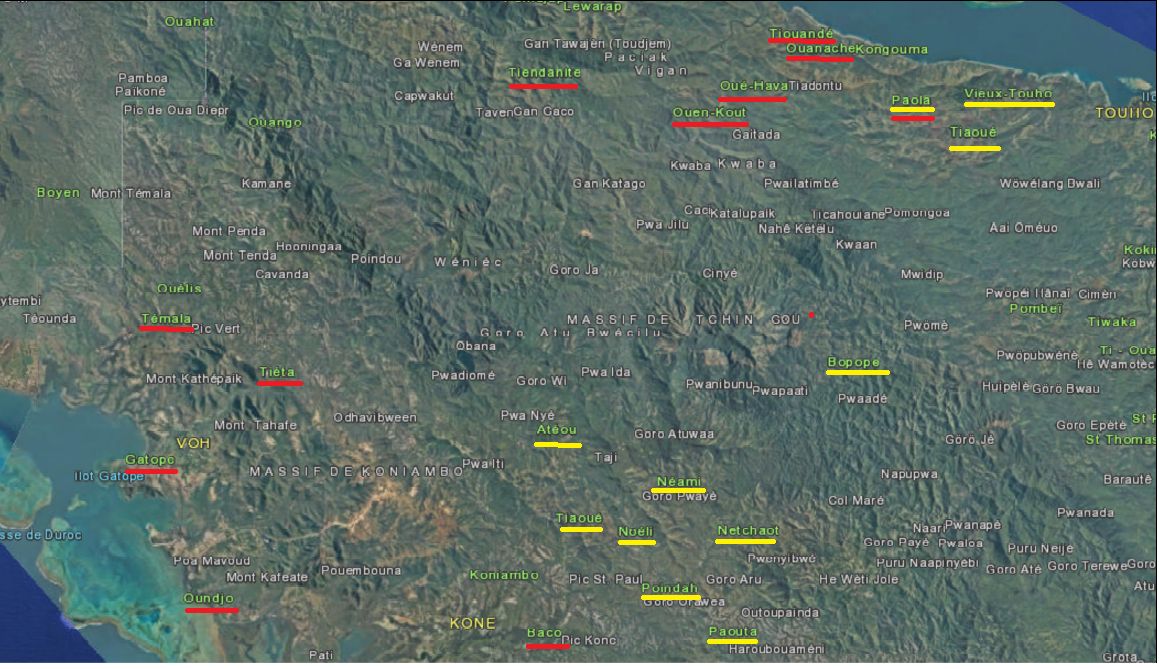
\includegraphics[width=\linewidth]{figures/map_languages.png}
 	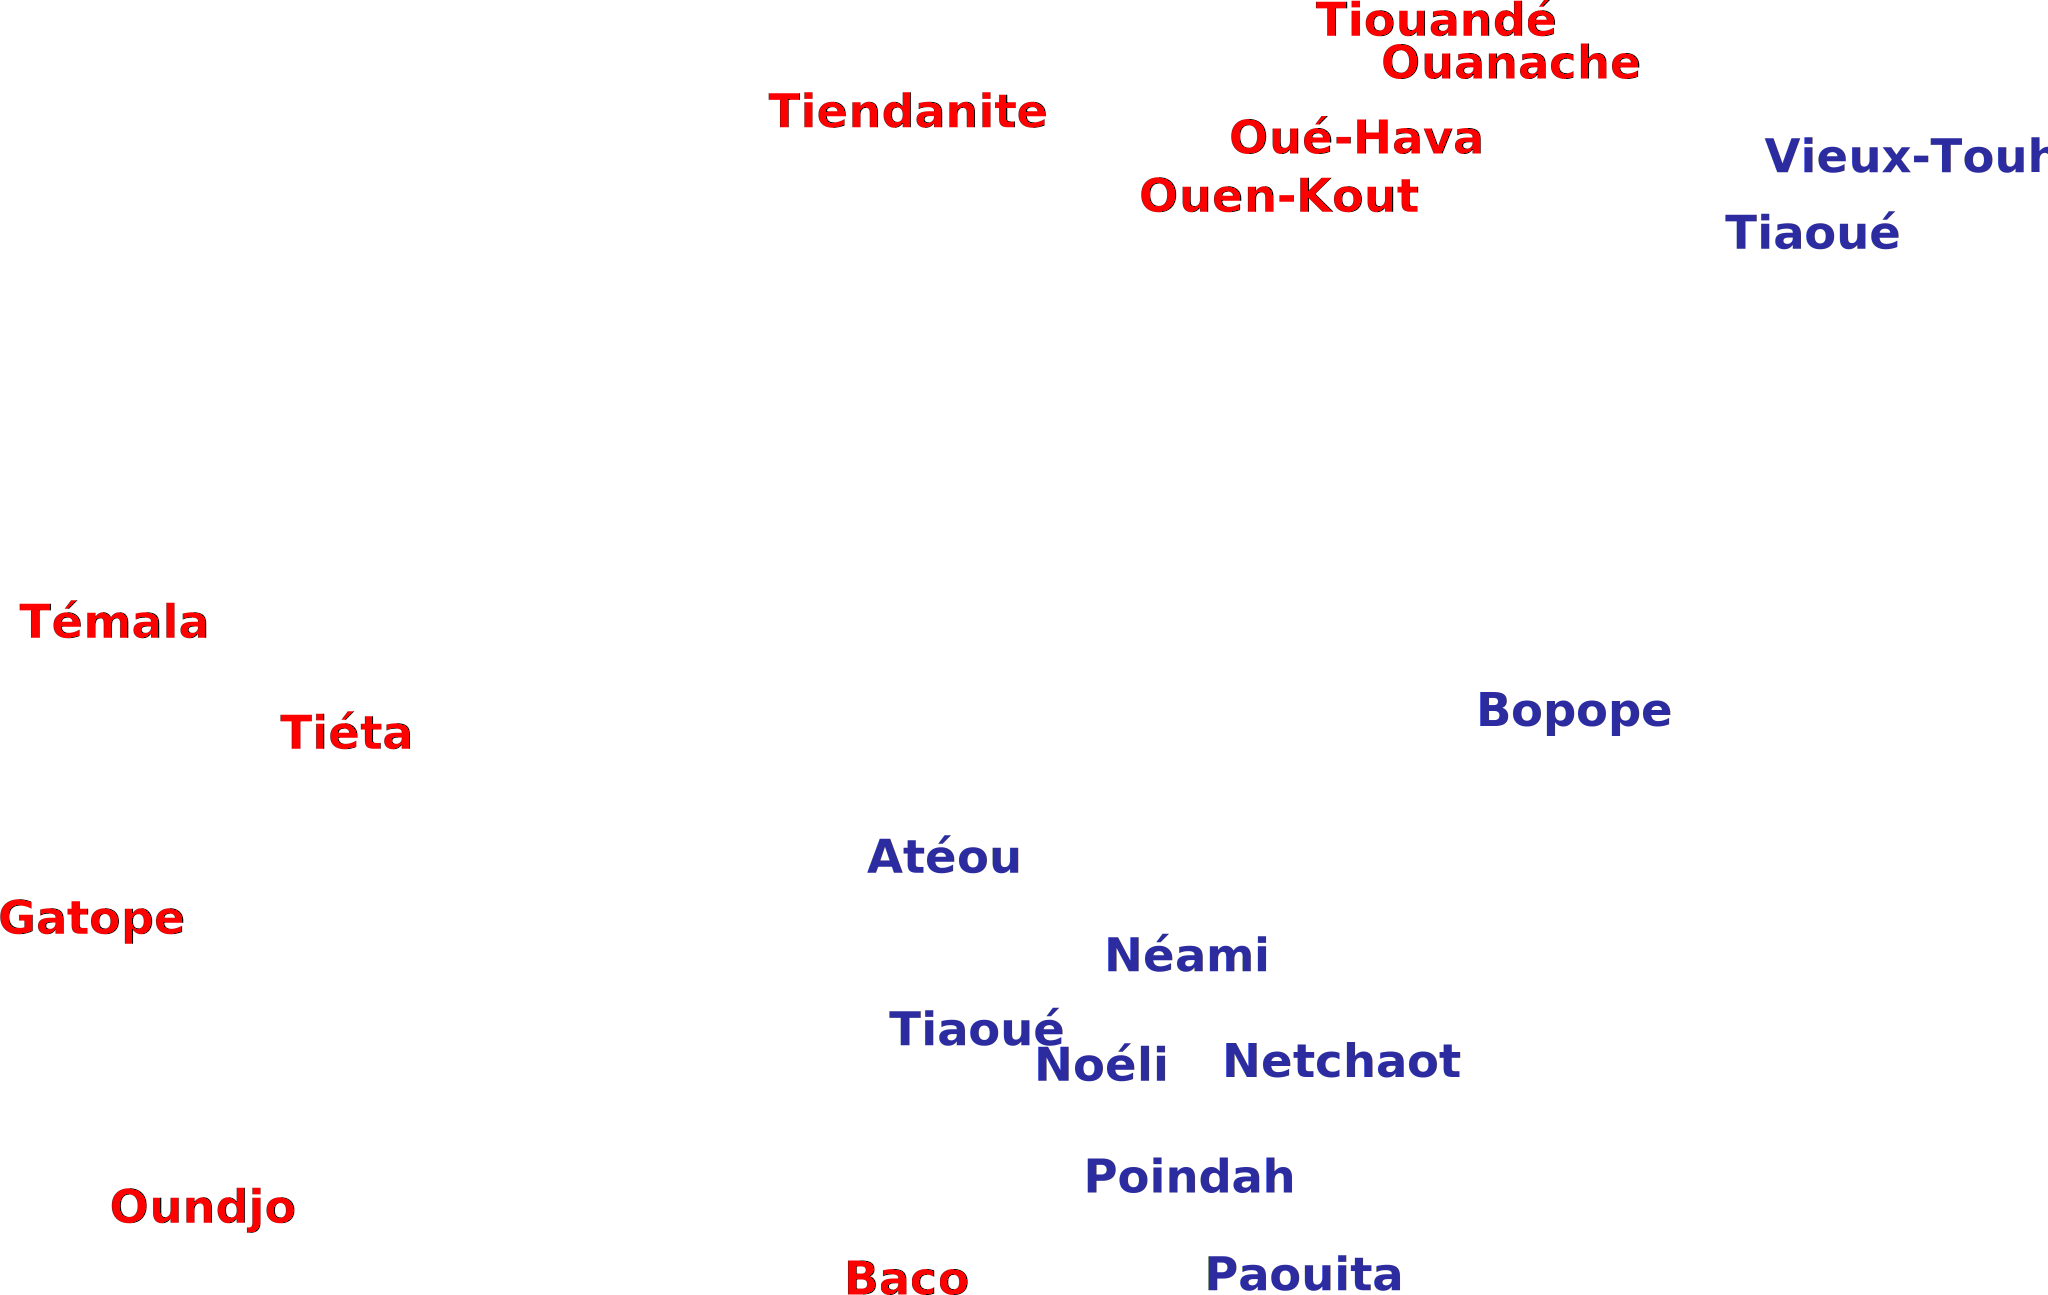
\includegraphics[width=\linewidth]{figures/vohkonepaicicemuhi.pdf}
 	\caption{Languages in the region, Voh-Koné-speaking villages in red, Paicî-Cemuhî-speaking ones in blue (adapted from \cite{gouvenementdelanouvelle-caledonie_explorateur_2019})\\\tiny © OpenStreetMap contributors. Tiles courtesy of Andy Allan}
 	\label{fig:map_languages}
 \end{figure}
 
 Vamale has been in contact with other, not readily intelligible, languages for centuries. %By providing a phonological description of the language, comparing the language to the rest of the cluster in depth will become possible. 
 It is surrounded by North Northern Caledonian languages of the Hienghène cluster, and Central Northern Cèmuhî, see \Cref{fig:map_languages}. While this is also the case for Haeke and Bwatoo (Haake), which mostly interact with Paicî, some Cèmuhî, and Pwaamei in the north, only Vamale is surrounded from all sides by non-Voh-Koné languages. Vamale has adopted the subject marker \textit{e=} \qu{1\gl{sg}}, as well as phonological traits from Cèmuhî (see \sectref{ssec:Vowel_Quality}), as well as loan phones from Pije. \citegen{leenhardt_langues_1946} description suggests that lexical changes have occurred. \parencite[162--168]{leenhardt_langues_1946}
 
 \begin{itemize}
 	\item \textit{da} \qu{who}, still used in western varieties, is now \textit{kai} \qu{who} in Vamale, and \textit{kaikai} \qu{for whom?} was substituted with \textit{nya(si/ko) kai}.
 	%\textit{xa} was a relativizer meaning \qu{X who does Y}, this is now \textit{a} like the unmarked one.
 	\item The indefinite articles have all changed: \textit{en} \qu{a, other}, still found as \textit{ven} in the Usa variety, is lost in Vamale, which now uses \textit{eca} \qu{\gl{indf}.\gl{sg}} and \textit{se} \qu{other}. \textit{men} \qu{\gl{indf}.\gl{pl}} and \textit{mun} \qu{\gl{indf}.\gl{du}} were used in demonstrative settings \parencite[165]{leenhardt_langues_1946}. Nowadays, putative equivalents would be \textit{ca} for the plural and \textit{muca} for the dual. 
 	\item There used to be more forms for adhortative exclamations (``vocative"), distinguishing adults from children (\textit{hai} and \textit{hnei}, respectively), whereas now there is only \textit{ha}.
 \end{itemize}
 
 \subsection{Multilingualism and variation}
 \label{sec:Multiling}
 \is{Code-switching}
 The author has met no-one between Téganpaik and Hienghène who speaks a Kanak language since birth without speaking another one. This is one of the first things someone will tell you: \qu*{I do Vamale a bit but also Pije and Fwâi}. People swear in three languages, they freely mix in words from other languages if they can't remember them, and they constantly code-switch functionally to mark their belonging to a group, to the description project, if they do not want somebody to understand, etc. This includes Usa, the variety spoken in Tiendanite. Speakers are able to adapt to coastal varieties, weave in Pije words, etc. In 2017, the author was present at the council of clans in Tiouandé, a monthly public meeting where all local affairs are discussed. I was there to give an update on the work. A conversation about a local criminal was done almost entirely in Pije, before the council switched back to Vamale. %Whether this was because Tiouandé is thought of as a Pije-speaking community, or because the criminal's clan is Pije-speaking, or, more likely, 
 This was likely due to privacy reasons, as they knew that I grasped some Vamale but no Pije. The choice of language among most middle age adults is functional and relatively free. There is thus probably no native speaker in the area who is not fluent or at least somewhat competent in another Kanak language. Male Cèmuhî speakers are an exception and usually only speak this one Kanak language; due to exogamy, many women come from another language area.
 
 \subsection{Neighboring languages}
 \label{ssec:neighbors}
 Vamale speakers have daily contact with other languages, most of which would not be readily intelligible. Pije is spoken in every Vamale-speaking village, and Cèmuhî by neighboring villages, as well as by local political authorities. Haeke, a Voh-Koné language, will also be discussed in some more detail below, not for its geographic proximity, but because the increased mobility of speakers has intensified contact with it. %An exception is Tiendanite-based Vamale Usa. It is very similar to Vamale, except for some archaisms, a different prosody, and some lexical differences.
 
 \subsubsection{Pije}
 \is{Pije}
 Pije (ISO 639-3 piz) is spoken in the same villages as Vamale. There is a coastal variety with about 70 speakers left; the Tipije varieties having all but disappeared due to the war. A mountain variety spoken in Tiendanite, called \textit{tha} \parencite[229]{haudricourt_langue_1968}, is relatively vital; it is the majority language there and practiced by many children (whereas Usa's youngest speaker is in her 20s). Pije is the most spoken indigenous second language of Vamale speakers. During elicitation sessions, Pije words were often given before being corrected. One reason for Pije's dominance in the area I'm focusing on is indigeneity: Pije is the land-owners' language here, the coast between Téganpaïk and Pedaa (Pindache) used to be in Pije-speaking hands, and a migration of Vamale speakers led to a complexification of the sociolinguistic situation. With the Vamale river flowing into the Tipije, language contact was always a fact of life in the upper valleys, but this contact has changed and intensified after the war. This also means that Pije is a language of prestige, the ``original" language, and many families reported a paternal (land-owning), Pije-speaking bloodline coupled to a maternal, Vamale-speaking one. Many residents were doubtful of the legitimacy of the project, as it should be Pije, more endangered and more autochthonous as it is, that should have been documented before Vamale. 
 
 \subsubsection{Fwâi}\is{Fwâi}
 Fwâi (ISO 639-3 fwa) is the language of Hye-hen (Hienghène, \qu{cry-walk}), the administrative center north of the Tipije river, and the school town of We Hava. The hospital, the market, an active cultural scene, and a bar, all attract residents of the three villages, and since the main road connecting Hienghène to the south runs through Tiouandé and Teganpaik, language contact is extensive. The main lexical influence seems to be swearwords, and the languages are not mutually intelligible.
 
 \subsubsection{Cèmuhî}\is{Cèmuhî}\largerpage
 Cèmuhi or Camuki (ISO 639-3 cam) is a tonal language with 3 register tones. It is spoken in the villages west of Téganpaïk up to Kokingone, and is the language of Great Chief Bouillant/Bwiyâ as well as most villages in the Great Chief's domain (to which most Vamale speakers belong). It is used for official purposes by the Great Chief's \textit{porte-parole} \qu{heralds}, and can thus be considered a regular contact language for Vamale, but is not intelligible with the latter and functional communication occurs in French. %The mayor of the commune's main town also speaks Cèmuhî, and uses it in poetry and stories he writes. 
 With around 3,300 speakers, it is one of the biggest languages in the area. 

 
 Vamale would have been surrounded by Cèmuhî speakers for some time before being moved to the coast. The villages Netchaot (Paicî\slash Cèmuhî) and Bopope (Cèmuhî), as well as the warring factions in the 1903 conflict Touho and Poyes, all spoke Cèmuhî. There was, however, a relatively stable and cohesive dialect chain of Voh-Koné languages from the west coast to Pamale, which suggests that for a while, contact happened eye-to-eye.
 
 \newpage
 \subsubsection{Haeke}\is{Haeke}
 \label{ssec:haeke}

 \begin{sloppypar}
 Haeke (ISO 639-3 aek) speakers, especially of the clans Wabealo and Cidopwaan, are tied through marriage to Vamale speakers, and according to Guiart, the mentioned clans claim to descend from the Paicî Naoutchoue/Naaucuwè lineage \parencite[92]{guiart_laire_1992}, with whom the Pei clan (important in Téganpaïk) is closely tied. Speakers of Vamale, thanks to cars, family ties (see the map \Cref{map:clans}) and frequent festivities, are now in more regular contact with other Voh-Koné varieties, especially Bwatoo and Haeke. However, the speakers the author spoke to were very aware of the differences between different speech practices and desirous to keep them distinct. Haeke is closer to Bwatoo and features typical Western Voh-Koné traits such as interdental fricatives, but as a funeral ceremony speech held in Haeke was understood by most Vamale speakers, some mutual intelligibility may be postulated. Haeke is highly endangered as well, and most contact happens in French. 
 \end{sloppypar}
 
 %\subsubsection{Conclusion}
 
 %Proud people, very motivated, but ridden with social problems and obstacles, hope that school will save the language, or other people.
 %That being said, the plural article \textit{ni} seems\begin{comment} to be a free variant of \textit{li}, and is used in all other Voh-Koné varieties.
 
 	%this is where we can maybe talk about their similarities and differences which has implications for what language is what language and what we consider the language we’re focusing on in this study and
 	
 	
 	
 	
 	%Other tips concerning politeness: avoid smelling food, always bring something (e.g. a package of rice) when invited to a meal, and know that the guest is supposed to eat first, then the men, then the women. If you stay for more than a day or two, offer to help with cooking and the dishes. Avoid touching the central post, leaning against a part of the house with a stretched-out arm, breaking a coconut indoors, and refusing anything offered multiple times, as this is as impolite as refusing any demand (for tobacco etc).
 	%
 	%Pei Dui's family, which comprises his woman from Maré, Élise and his daughter whom he had with a Paicî woman and who is in a boarding school in Poindimié, Elodie, moved from a small concrete house now cluttered with stuff, mostly papers, next to the concrete foundation (a concrete disk with a hole for the central post) of a torn down hut, to an empty house uphill of his adoptive mother's house and his adoptive brother Richard's house, who has a roofless hut next to it, the straw for which has been dry in his garden since 2013. Dui's new house was built with subsidies, the surrounding ground is rubble, Yaté the dog would guard it if she weren't so sweet. 
 	
 
 \section{Previous work}
 \label{sec:prev_work}
 \largerpage
 Vamale is almost exclusively an oral language. It is used in church (at least in Téganpaïk) for songs; Néa Galé of Baco has published some prose, and some songs are archived, recorded by Haudricourt in 1963 \parencite{nea_poesie_1963}. 
 The Protestant missionary and pastor Maurice Leenhardt was based in Houa\"ilou, but was active across the entire archipelago and wrote extensively about Kanak languages and cultures. His most important linguistic work is \textit{Langues et dialectes de l'Austro-Mélanesie}, published in 1946. Short grammar sketches on almost every language at the time are followed by a comparative word list of over 1,000 items. This is the most extensive work done on Vamale (``\textit{'Moaeke}") to this day. While a number of items were deemed by speakers to be loans from other languages, mostly Pije, the list is the only published trace of the names of gods, dances, and objects since lost.
 
André-Georges Haudricourt worked in New Caledonia between the 1940s and the late 1970s. The relevant articles are overviews over the phonological systems of all then-described languages (\citeyear{haudricourt_richesse_1961}), and grammatical typologies of the archipelago (e.g. \citeyear{haudricourt_langues_1948}, \citeyear{haudricourt_new_1972}, \citeyear{haudricourt_langues_1948}). Haudricourt's only work on Vamale, a dictionary project, was never published and is presumably lost \parencite[18]{rivierre_bwatoo_2006}. 

 %\todo{short descriptions}
 Jean-Claude Rivierre worked on Paicî (\citeyear{rivierre_dictionnaire_1983}) and Cèmuhî (\citeyear{rivierre_langue_1980}, \citeyear{rivierre_tonogenesis_1993}), as well as on Bwatoo (\citeyear{rivierre_bwatoo_2006}, a grammar sketch of 45 pages with a detailed dictionary following), and was the most important author on Vamale's immediate neighbors (e.g. \citeyear{rivierre_contact_1994}). He also assembled a precious dictionary of Hmwaveke containing Vamale items, unfortunately not yet published: \citetitle{rivierre_projet_}.\largerpage

%\subsubsection{Cannibalism}
%\is{Cannibalism}
%Cannibalism is a notorious part of traditional Kanak society. Although not directly relevant to the description or documentation of the language, the author believes it justified to say a few words about this stigmatizing and widespread connotation of the word ``Kanak". 
%Cook reports an aversion to cannibalism in Kanaks in 1774 \parencite[56]{sand_reconstructing_2000}. LaPérouse describes a cannibalistic population at constant war in 1788  \parencite[58]{sand_reconstructing_2000}. According to \citeauthor{bensa_political_1997}, a chief's power was based on the number of bodies controlled relative to neighbors. Following this, the destruction of enemies' bodies was one of the bases of chiefdom\is{Chiefdom} \parencite[89]{bensa_political_1997}. One reason for consuming the enemy is to avoid vengeance from the ghost of the departed. Destroying the corpse, according to \citeauthor{bensa_political_1997}, was seen as a way to prevent the deceased from becoming an ancestor, who counted as a body controlled by the deceased's clan, and would thus not have diminished the neighbor's power. But even this destruction does not seem to have been a total safeguard against revenge, since eating enemies happened outside of inhabited areas, to prevent villages from being haunted \parencite[96]{bensa_political_1997}, and \textit{nyawan xhwi} \qu{ghost of an eaten person} plays a role in folklore. 
%
%A word of caution: as Sand mentions, Kanak societies underwent traumatizing changes upon contact with Europeans \parencite[322--323]{sand_what_2007}. Illnesses brought by outsiders decimated the population to such an extent\footnote{80-95\% losses are common in the Pacific \parencite[329]{sand_what_2007}, \parencite[2, 3, 11]{kirch_long-term_2007}
%.} that it is doubtful that societal structures remained unaffected (compare the Black Plague of the 14\textsuperscript{th} century in Europe). In fact, an intensification of war and cannibalism was attested for Grande Terre in 1840, citing as the cause the belief that the new diseases were the result of hostile magic from neighboring groups \parencite[318]{sand_what_2007}. However, while the first documented contact occurred in 1774 with James Cook, colonization only happened in 1853, leaving ample time for whalers, slavers and other sailors to land on Caledonian shores, and for epidemics to spread. For this reason, pre-colonial and pre-contact society are not the same concept.
%%I have met most members of the Pei clan, of whom a member was, in 1999--2017, the cultural coordinator of the municipality of Touho. Dui is the link between the State’s administration and the local customary authorities. I spent three weeks in his home. He introduced me to several of his friends who showed a keen interest in documenting, and if possible preserving Vamale. They and others have been invaluable in finding speakers, reviewing transcriptions, and legitimizing the project in the eyes of the community. I hope that their involvement will make it easier for other members to join the project.


%high chief is Cèmuhî-speaking, Pamale used to have its own High Chief, what this means for language attitudes, nostalgia, and why people would rather be silent than taint the glory of the past by making mistakes or using loan wordsxx


%\section{Conclusion}
%
%Now that we know what specific variety is the focus of this thesis, how the language fits into existing classifications, and are somewhat better informed of its context, we can go on to the first part of the main point of this grammar: the phonology of Vamale.

\begin{center}
	\textit{ma gavwe xaleke, ka caihnan.} \qu{May you see, and know.}
\end{center}


\begin{figure}
	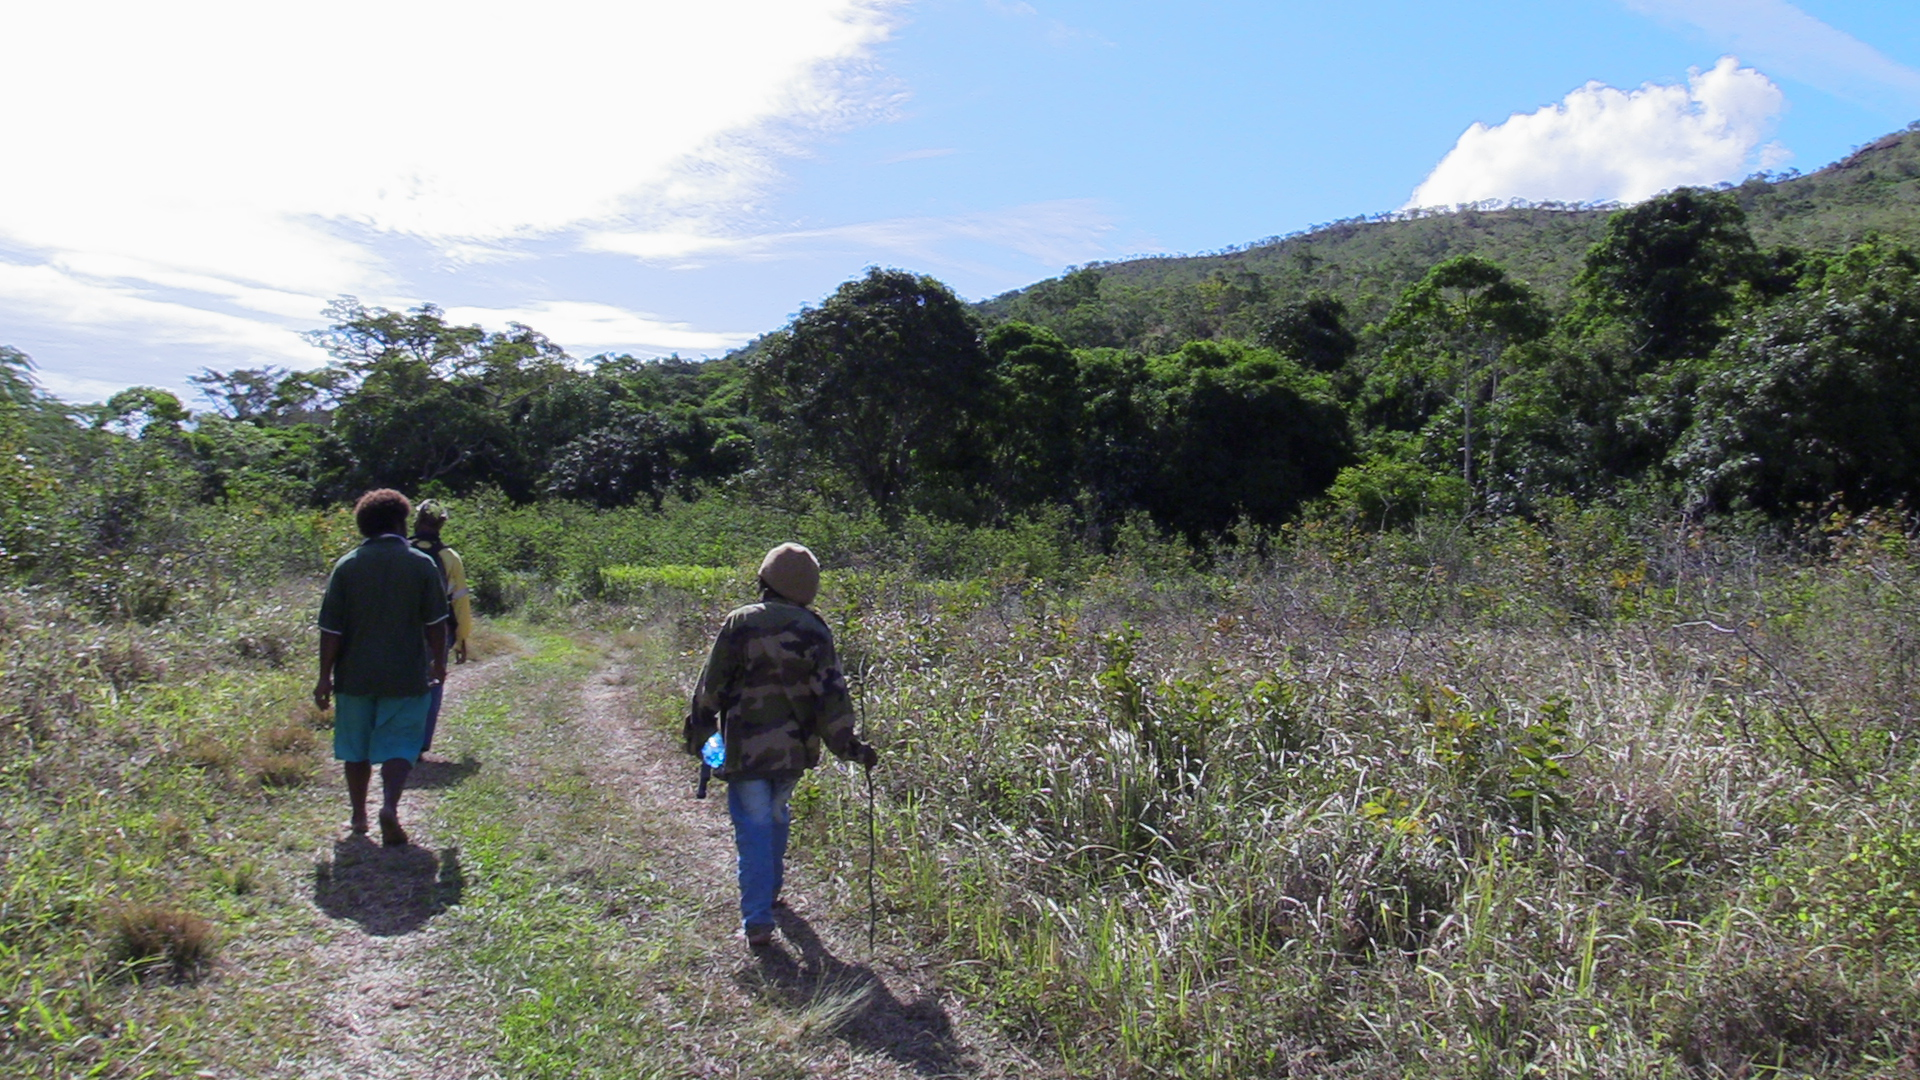
\includegraphics[width=\linewidth]{figures/bande}
	\caption{Mr.\ Pei and Mr.\ Kalène on the path to Wanaa}
\end{figure}


\chapter{History of speakers}
%The history of the language family’s speakers starting from some point in history that will eventually lead in not that much detail to the change in the education system that was a significant contribution to the decrease in the speaker population. This leads to the more recent historical and also current situation of what languages are spoken where in the region, how transportation changes have affected their interactions, etc., which leads into the 
%\subsection{History}
\label{chap:Tipije}
\largerpage
Knowing the history of the speech community helps to understand the length and intensity of exposure to today's contact languages, and to identify possible past dwelling places of speakers. The exact history of Vamale speakers is poorly studied. This section mainly aims at reconstructing the approximate distribution and the contact languages prior to the major population movements of 1904 and 1917, and to give a brief overview of the reasons why the language lost so many speakers.
The account given here is different from the situation described in detail by \textcite[91--93]{guiart_donnees_1984}, and yet different from \textcite[20]{leenhardt_evenements_1978a}, partly because most clans have changed names. The following is a summary of written and oral sources; some details remain unclear.

\section{Pre-1917}
Pamare (the Paicî name)/Pamale/Vamale is the name of a river tributary to the Tipije, flowing northwards from (Na Unu) Pamale mountain, just southwest of the Cigu \~ Tchingou massif. Oriented almost exactly south-north, it flows from an area today uninhabited and bordered by Cèmuhî speakers (see \figref{map:pamale}), until it unites with the Vawe river,\footnote{The Vawe tribe is mentioned in \textcite[26]{leenhardt_figures_1978} as well as in \textcite{sand_tiouande_2001}, and the Pei and Fouan clans claim to be from there.} at a river bend and becomes the Tipije \~ Tipindjé river, joined after a few kilometres by the Usa creek. 

\begin{figure}
% 	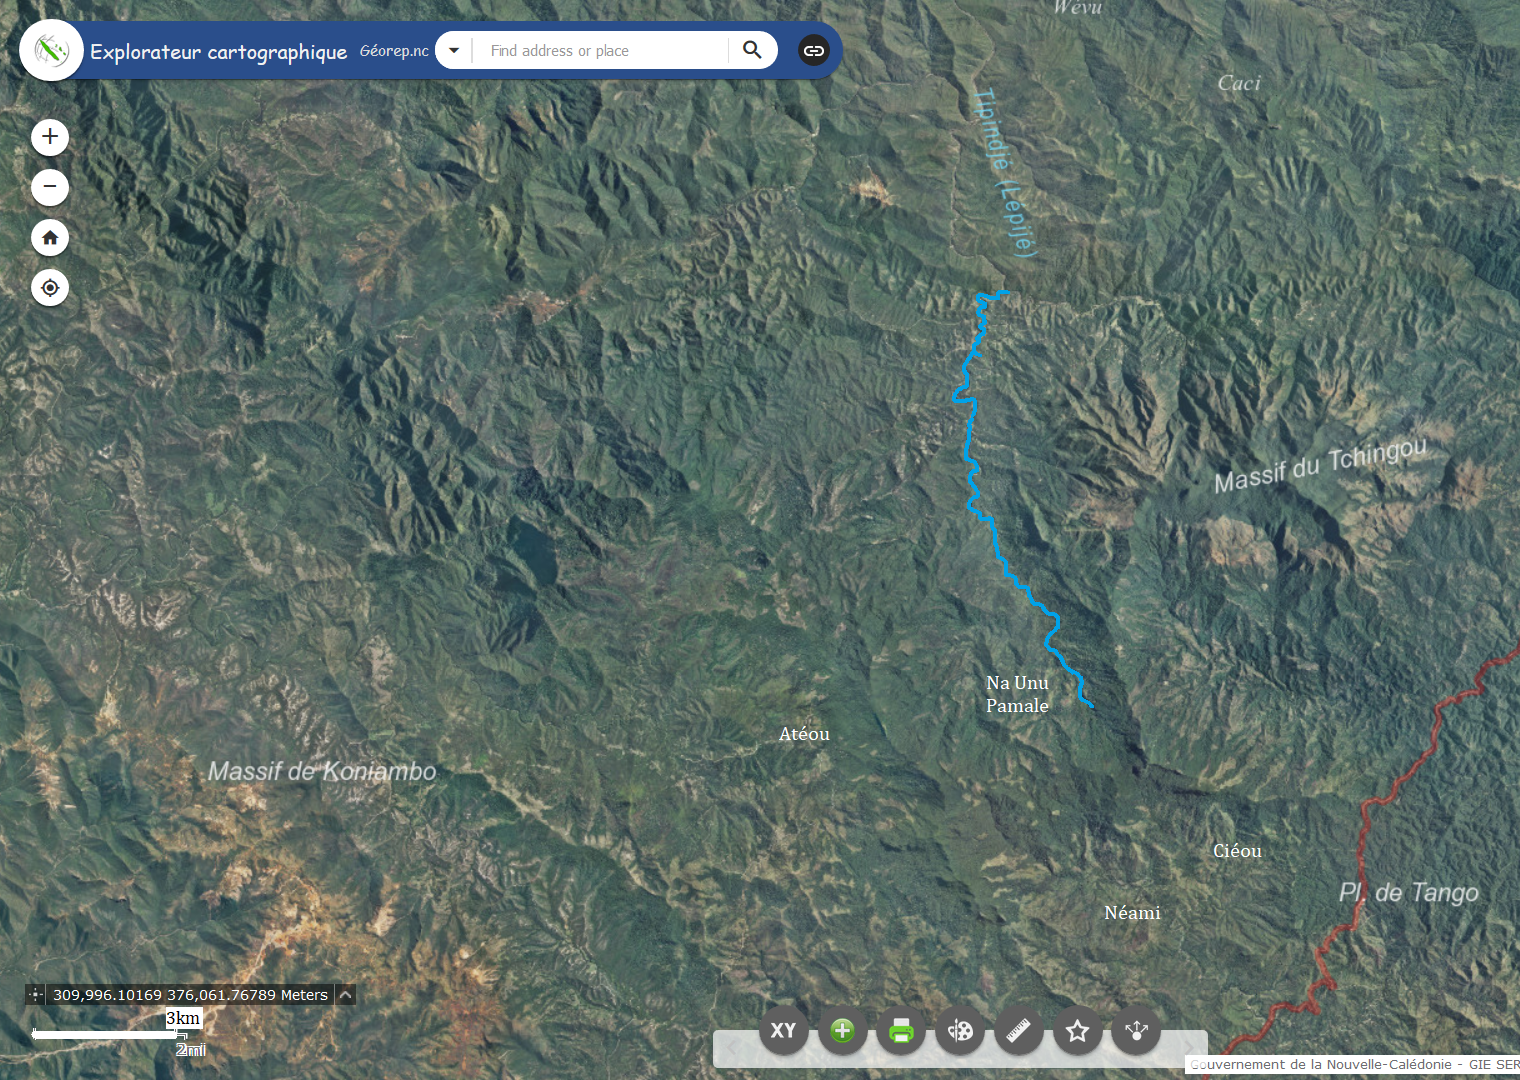
\includegraphics[width=\linewidth]{figures/ye_olde_mappe2}
	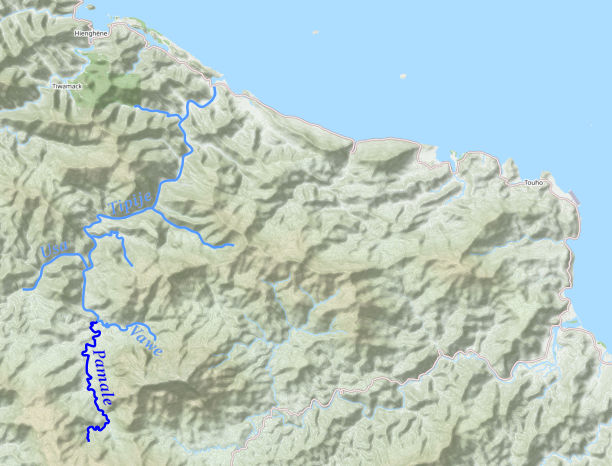
\includegraphics[width=\linewidth]{figures/pamale.pdf}
	\caption{Map of the Pamale river}
	\label{map:pamale}
\end{figure}

The Vawe, Pamale, and the upper Tipije valleys are said today to have been inhabited by Vamale speakers. Pamale is said to have been a great chieftaincy \parencite[59]{gohoup_guerre_2008}. The North of the island, roughly north of the Cèmuhî domain, was loosely structured into two alliances: \textit{Hoot} \qu{great tide} and \textit{Whaap} \qu{raven}, today eponymous of the customary area \textit{Hoot ma Whaap}. The Tipije valley was \textit{Hoot} but the later refuges of Pamale people, Wanas/Wanaa, Temala and Tiéta, were \textit{Whaap} \parencite[6]{guiart_lorganisation_1954}, so a cautious assumption may be made that Pamale refugees followed old paths of alliance. See \Cref{map:clans} for a visual representation of Guiart's analysis. %On the other hand, the Pamale refuge \textit{We Hava} is in the middle of the \textit{Hoot}-aligned Tipije and used to be ruled by Pamale's traditional ally\footnote{\parencite[272]{guiart_evenements_1970}} Kafeyat Batepoanwhane/Batpawan/Cidopwaan \qu{Nametaker Erect-Phallus}, who could retreat to Ouiou (\textit{Wévu} on map \ref{map:history}), which is relatively far upstream and quite likely \textit{Hoot}. 

\begin{figure}
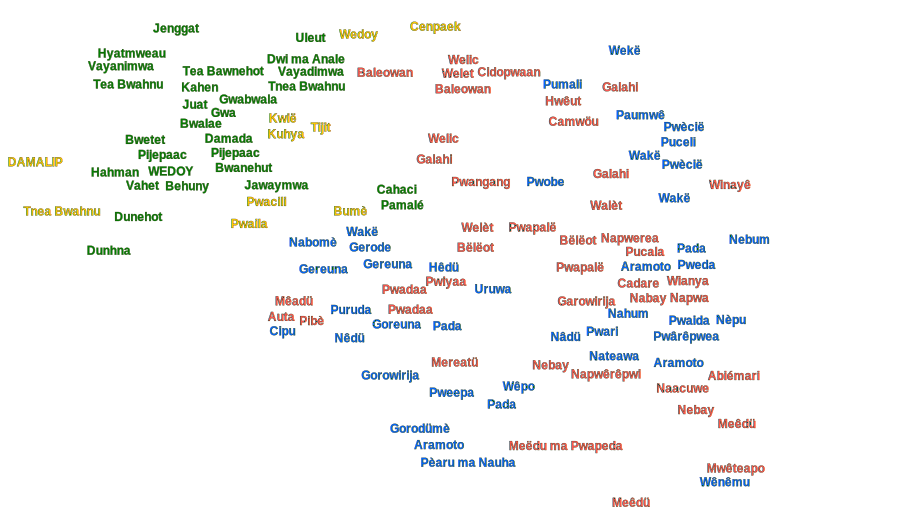
\includegraphics[width=\linewidth]{figures/clans_blur.pdf}
\caption{Selection of precolonial clans adapted from Guiart's 1979 map \textit{Clans autochtones: Situation pré-coloniale}, %with black underlines for yam masters, red for sun/rain
%masters, purple for taro masters, and dark brown for thunder masters,
green highlights for Hoot and yellow for Hwaap lineages, red for Bai and blue for Dui. \parencite[71]{guiart_clans_1981}}
\label{map:clans}
\end{figure}

The local distribution of languages before the 19\textsuperscript{th} century is difficult to estimate. However, around the turn of the last century, the land between the Cigu mountains and Koné, south of the Hienghène and at least up until Wan Kuut is likely to have been speaking varieties of Hmwaeke/Vamale. Clans speaking it almost certainly formed minority speaker populations in the allied valleys of Wanaa(s) (Ouanache), Thexhwaade (Tiouandé), We Hava, Pwey (Poyes), and on the other side of the mountains in Temala, Ceta (Tiéta), and Koogo (now deserted), as frequent exchanges were maintained with these villages, and this is where the refugees went (see \Cref{map:fugitives}). The chiefs of Wanaa and We Hava spoke Vamale \parencite[20]{leenhardt_evenements_1978a}.
\begin{figure}
% 	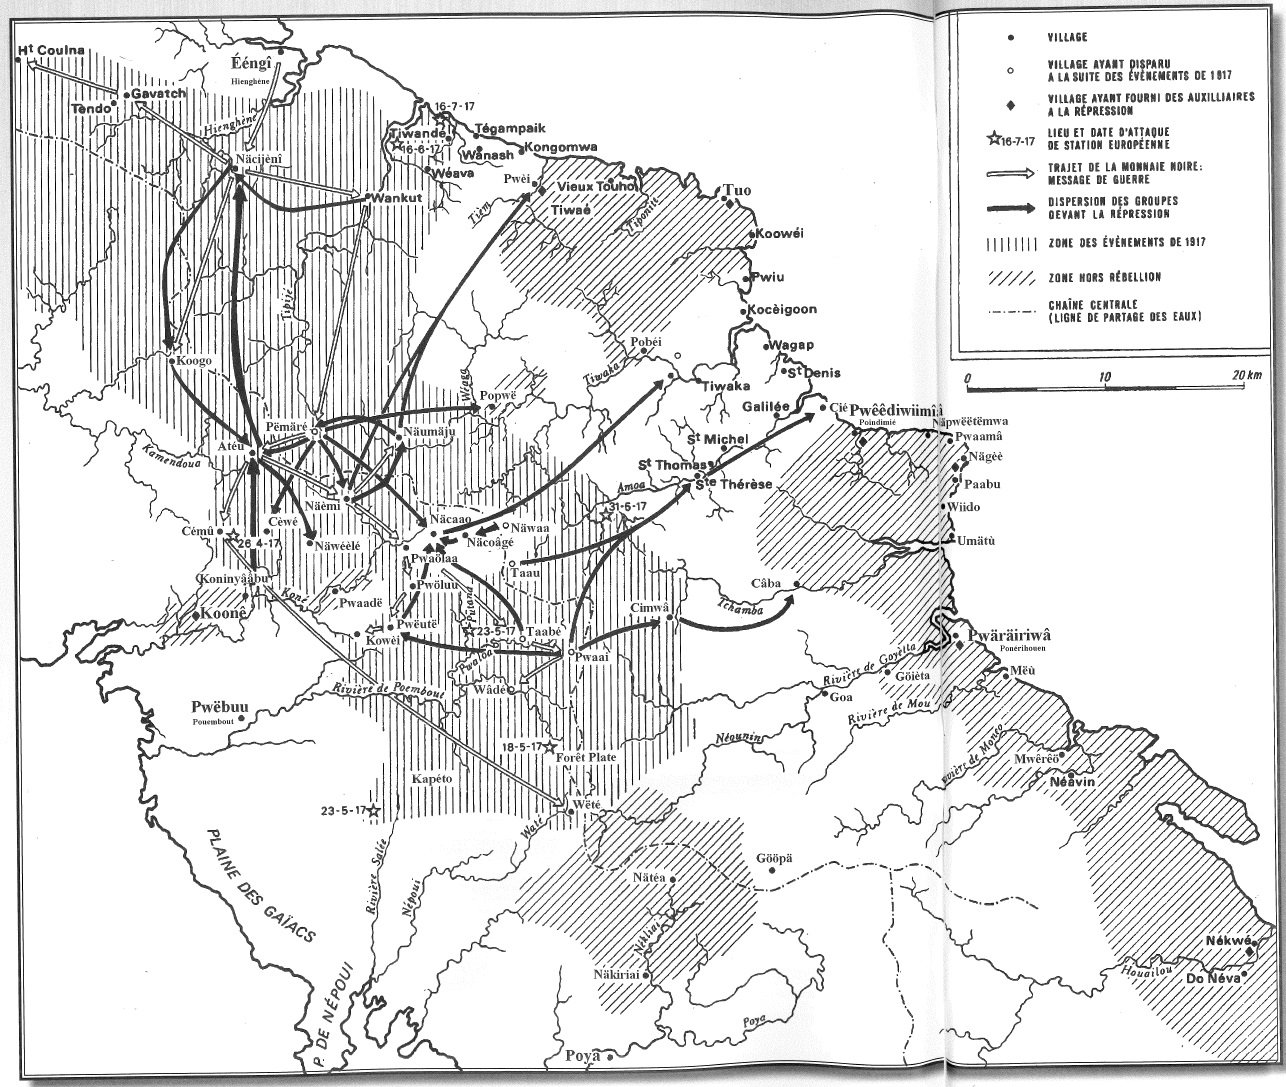
\includegraphics[width=\linewidth]{figures/prov_map_fug}
	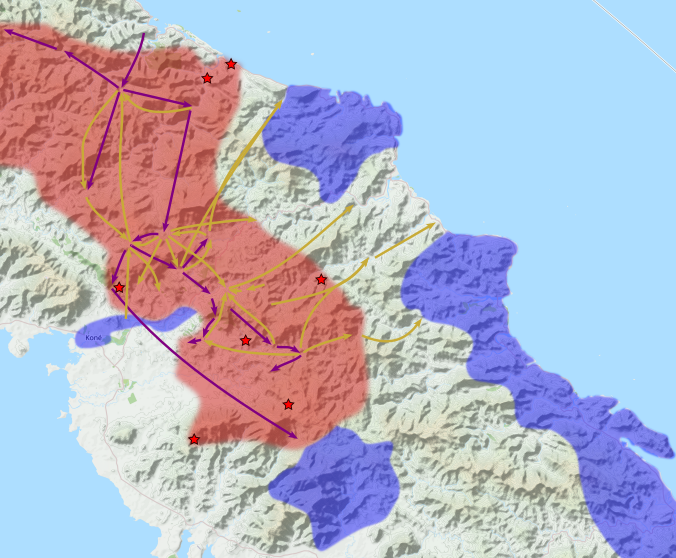
\includegraphics[width=\linewidth]{figures/refugees.pdf}
	\caption{Main movements of refugees following 1917 \parencite[7]{bensa_1917_2008}. Many movements leave Pamale (``Pëmärë").}
	\label{map:fugitives}
\end{figure}

%\begin{figure}
%	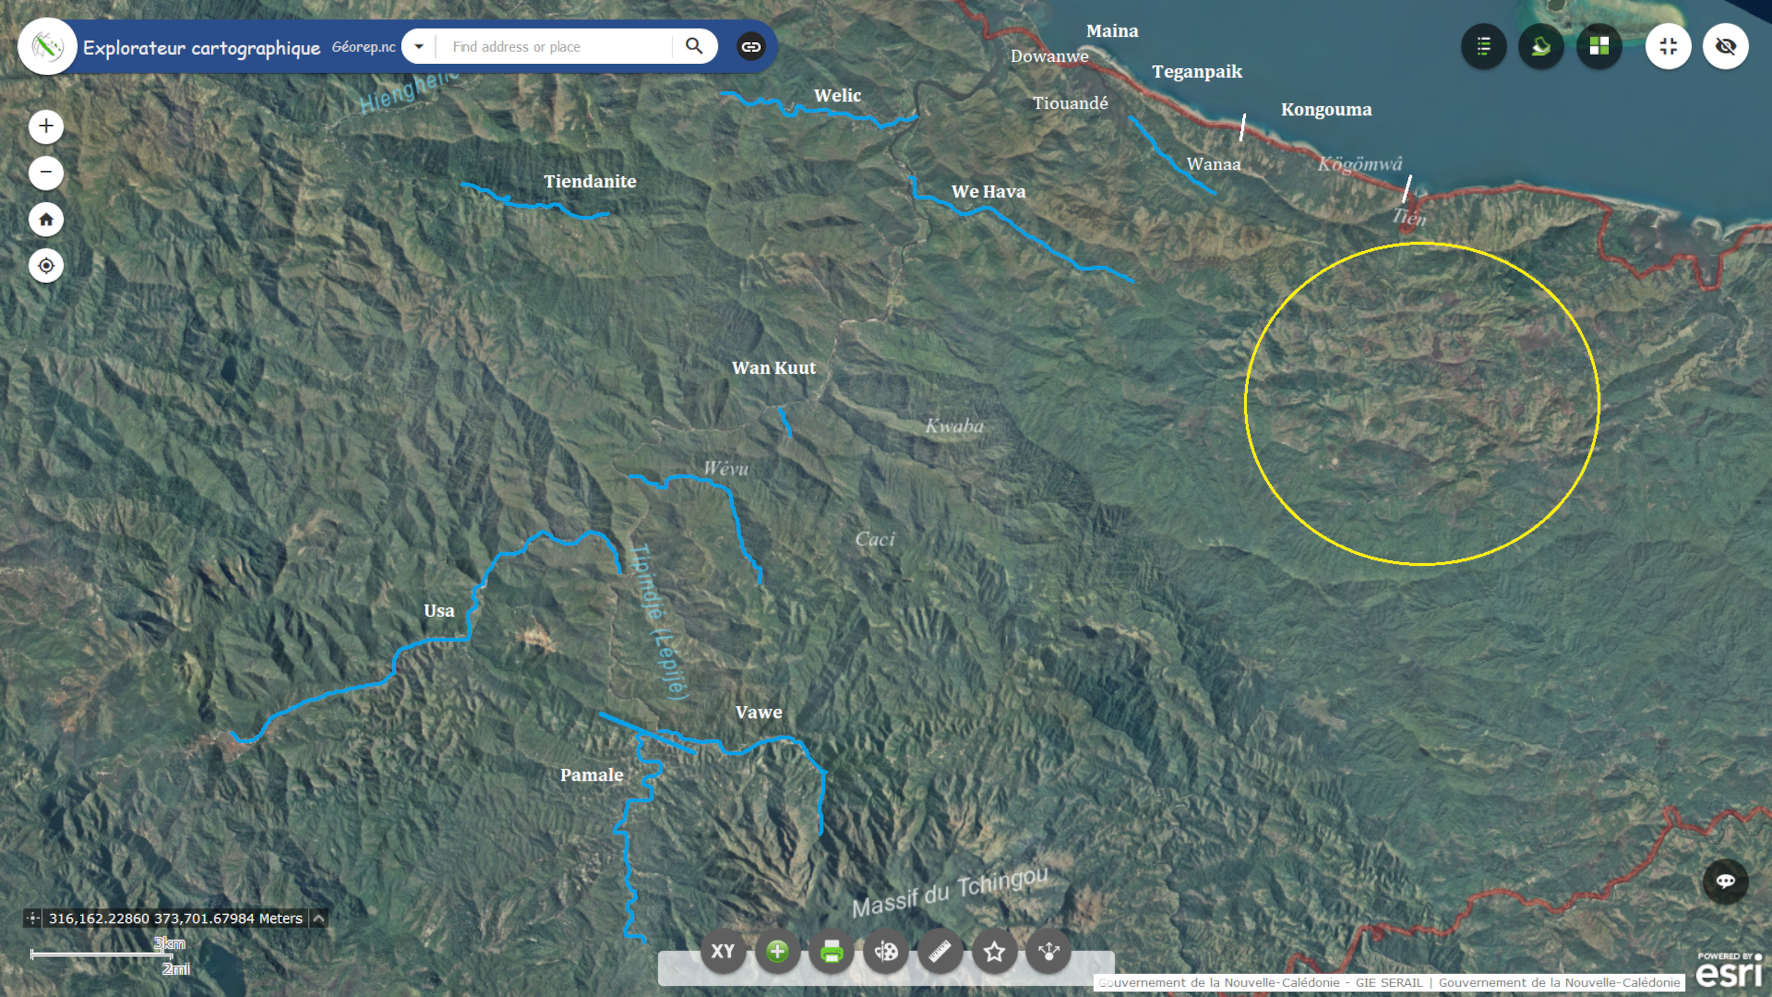
\includegraphics[width=\linewidth]{figures/ye_olde_mappe_politics}
%		\caption{Map of the area with main valleys. Poyes is circled in yellow. \cite{gouvenementdelanouvelle-caledonie_explorateur_2019}}
%	\label{map:history}
%\end{figure}

\section{The 1917 War}
On May 10\textsuperscript{th} 1901, a peace meeting took place in Pamale (\textit{Paix de Pamalé}). At the time, the area was not yet directly concerned by land spoliations or missions, though oral accounts speak of Pamale as a refuge for people driven from their lands \parencite[368, 369]{bensa_sanglots_2015}. The parties discussed the ``Affair of Poyes", a conflict between war chief Amane of Poyes and chief Hippolyte of Touho. Whatever the real reason was -- a woman, capitation tax, cooperation with Europeans, or land -- the two reconciled. \is{Affair of Poyes}

On the one side was Amane, a powerful war chief in the Cèmuhî-speaking village Poyes, who claimed land all the way till Paola on the west coast, according to a police report \parencite[24]{leenhardt_figures_1978}. He was a brother of Bwiyang, chief of Poyes. According to Amane himself, he had been promised since birth a woman whom Hippolyte of Touho took for himself. Amane wanted her back. Another explanation is the difference in stance towards Europeans. Hippolyte was Catholic and in close cooperation with European missionaries. Due to his exposed situation on the coast, his father Napoléon had already been in contact with Europeans, whereas Poyes remained relatively independent \parencite[21]{leenhardt_evenements_1978a}. According to (Protestant) Leenhardt, Hippolyte ruling over a militarily weak tribe \parencite[28]{leenhardt_figures_1978} was manipulated by the local Catholic missionaries, the peace meeting was an overreaction and the Poyes had not even attacked yet. It may also have concerned the capitation tax \parencites[23]{leenhardt_figures_1978}[13]{philcat_revolte_1989}, which Amane refused to pay, whereas Hippolyte cooperated with the occupier. In any case, Amane met with his adversary, and Governor Paul Feillet, the missionary Maurice Leenhardt, as well as Kanak dignitaries from as far away as Houailou, for a peace palabre \textcite[24]{leenhardt_figures_1978}. The two reconciled. 
After the peace meeting, the \qu{Thunder of Poyes} Amane held several reunions in Pamale. 

Possibly in response to this subversive behavior \parencite[289]{saussol_lheritage_1979}, or because Pamale was a safe haven for refugees, the Pamale lands' reservation status was revoked by the government by the (unpublished) \textit{arrêté} n°775 on June 30\textsuperscript{th} 1903 \parencite[282]{guiart_evenements_1970}, enacted on July 30\textsuperscript{th} 1904 \parencites[92]{guiart_laire_1992}[22]{philcat_revolte_1989}. %\todo{check}

The reservation status had been Pamale's only protection from state-sanc\-tioned spoliations \parencite[3]{demmer_nationalisme_2003}, and the land was bought by the Belgian cattle rancher Charles Metzdorf. He founded a cattle ``station", a ranch, at Pamale \parencite[273]{guiart_evenements_1970}. The same year, possibly to avoid conflict with the population, Metzdorf's manager brought in \textit{gendarmes} who burned the houses of the Pamale, as well as the houses and the Protestant temples in Pije-speaking Pupay (Puepaek) and in Paada, and the village of Pwekea Kalemumak (upper Voh valley, probably Haveke-speaking) \parencite[266]{guiart_evenements_1970}. This act of war may have targeted clans who were allied to Pamale families and their neighbors, and who could have taken in refugees. Governor Feillet claims his group arrived on Charles Metzdorf's cattle-station in Pamale on the 10\textsuperscript{th} of May 1901 and slept in the recently abandoned cattle station in Vawe\is{Metzdorf, Charles} \parencite[26]{leenhardt_figures_1978}, both of which can only have existed legally 3 years later, after Pamale was erased from the map with fire and guns, as mentioned above \parencite[27]{leenhardt_figures_1978}. Governor Feillet cannot have confused the dates because he left for France on October 18\textsuperscript{th} 1902 and died in Montpellier September 2\textsuperscript{nd} 1903 \parencite[29]{leenhardt_figures_1978}. Whether Metzdorf came earlier than officially claimed and then had the reservation revoked in order to avoid neighborly conflicts with the dispossessed former inhabitants could not be reconstructed by the author. Metzdorf would later leave the area to be succeeded by the Ouaco mining company. It, too, left by the early 1930s \parencite[266]{guiart_evenements_1970}. The land is now in customary hands and used as hunting grounds by the villages Néami and Noéli.

%\begin{figure}
	%\centering
%	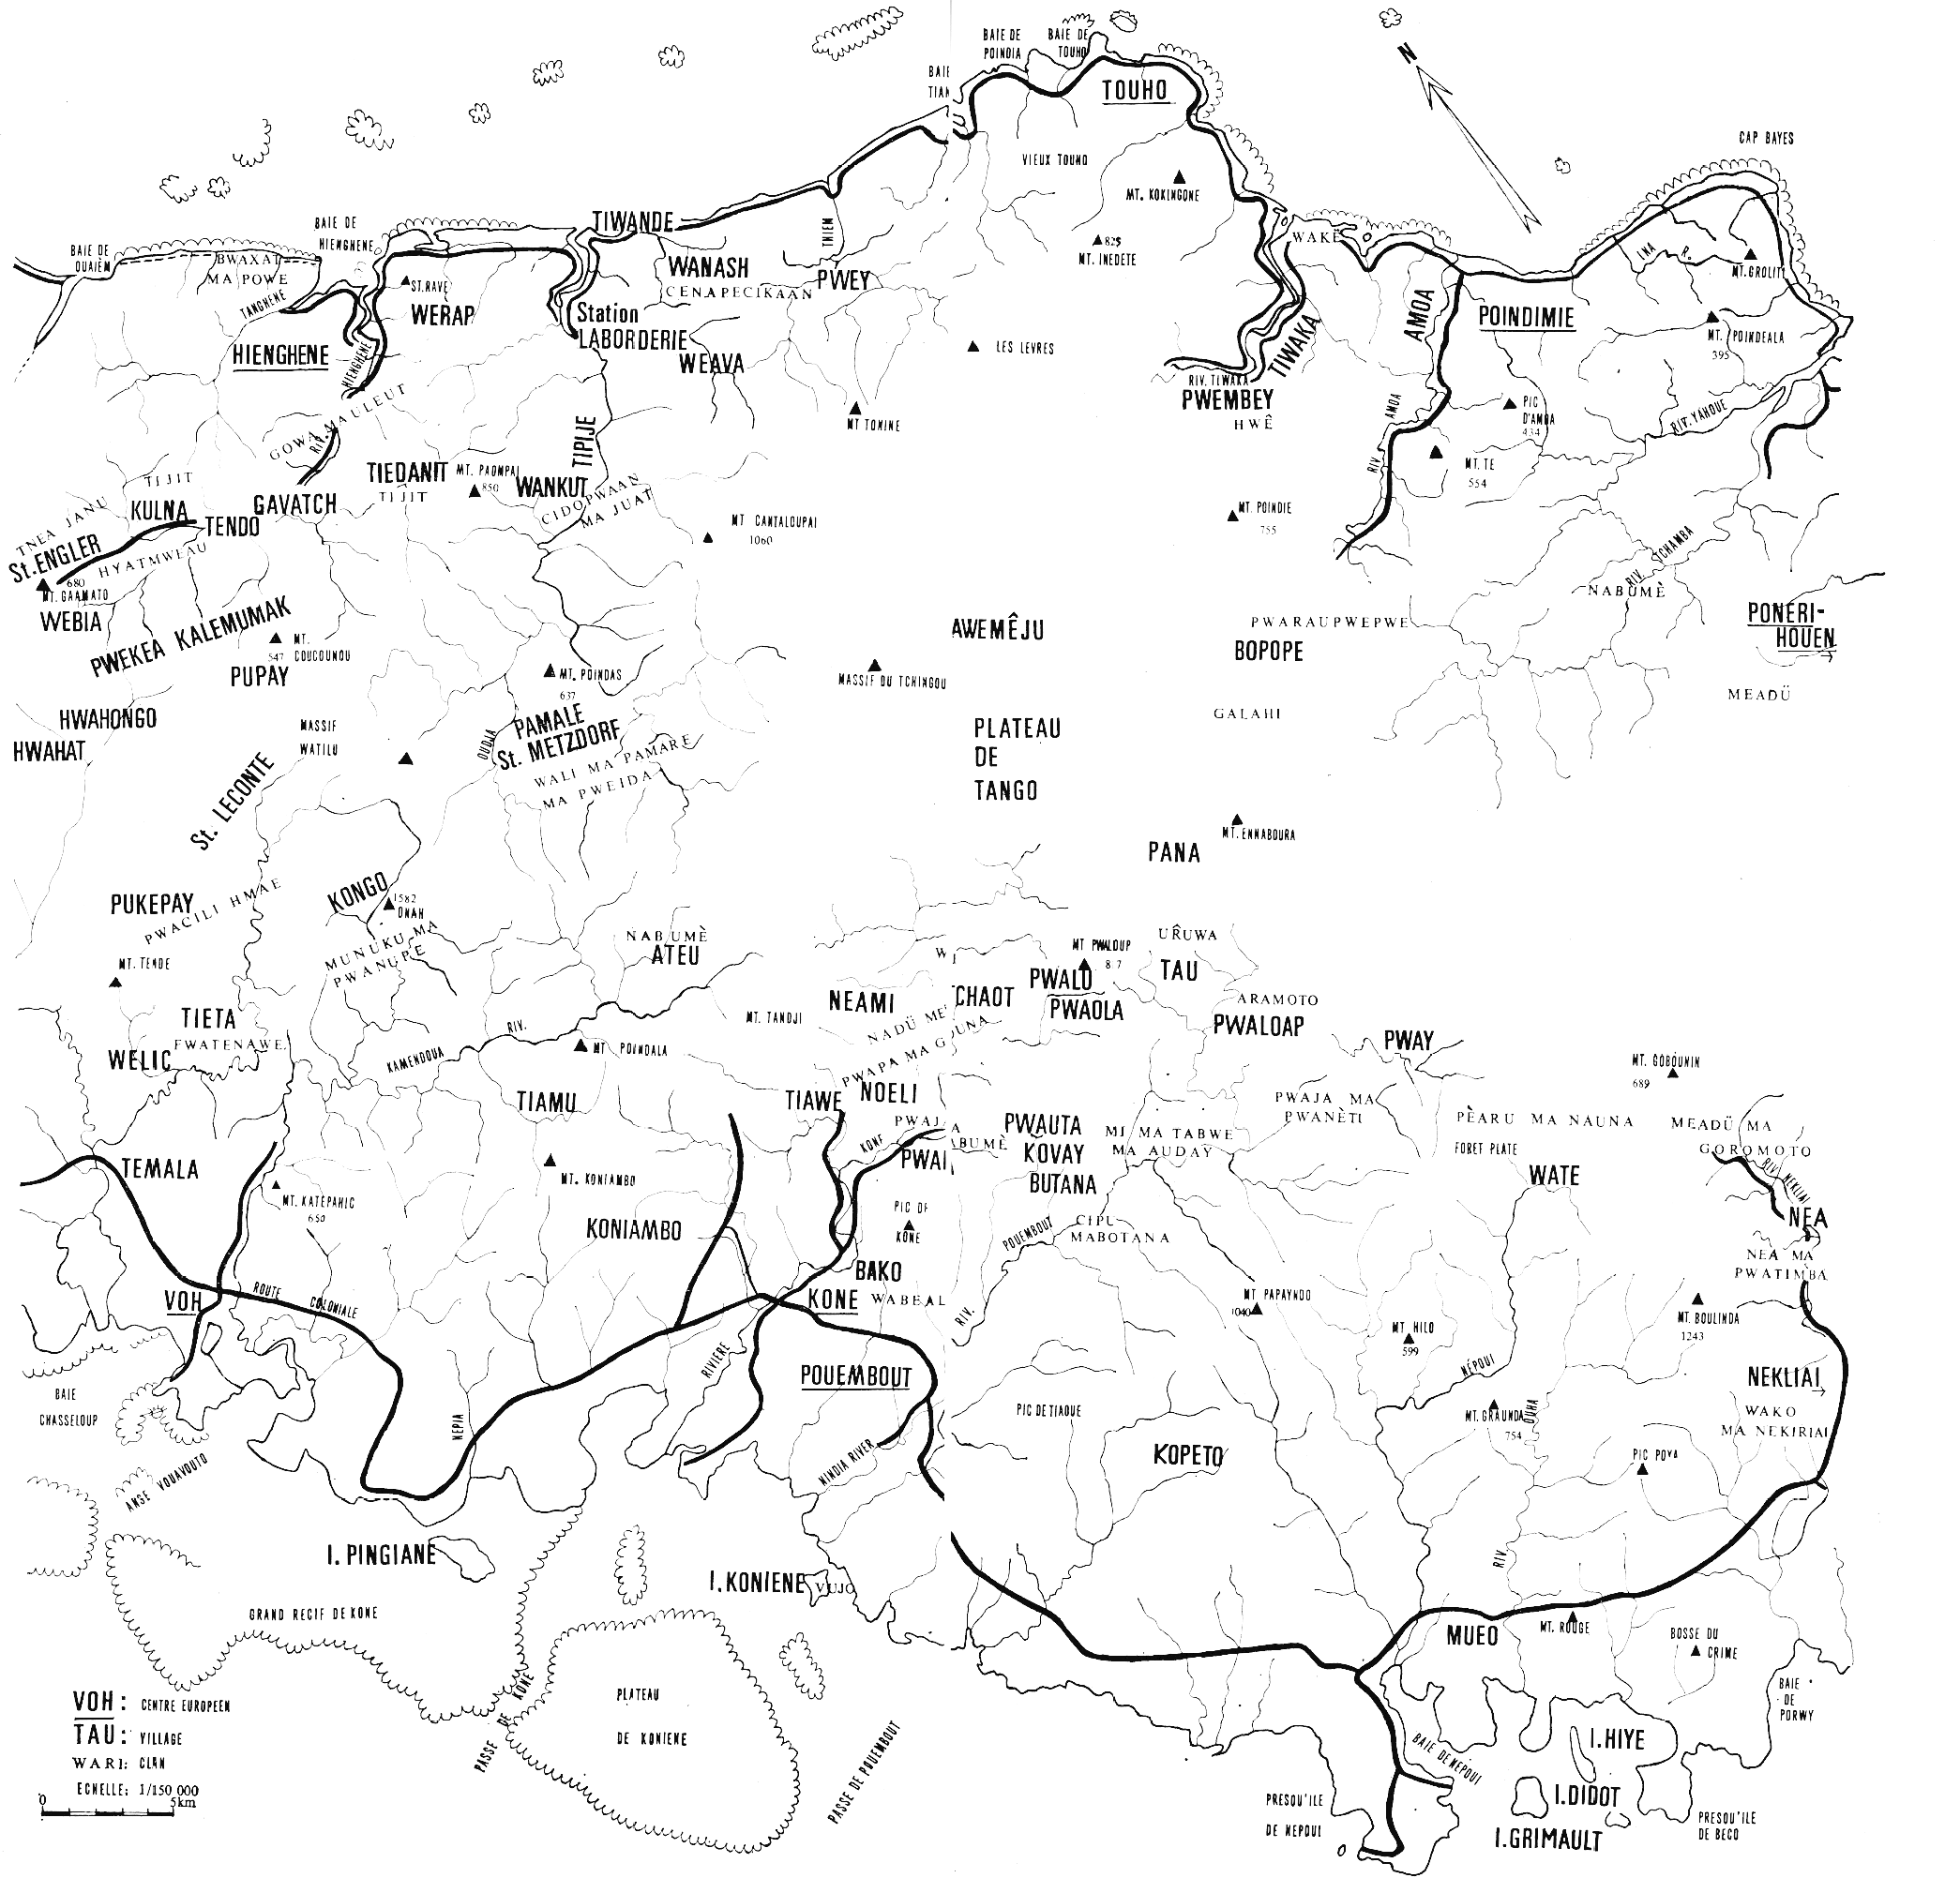
\includegraphics[width=\linewidth]{figures/pamale_guiart}
%	\caption{A map of main Kanak villages around 1913 \parencite[269]{guiart_evenements_1970}}
%	\label{fig:Guiart}
%\end{figure}

As a reaction to the destruction of their houses, the Pamale tribe,\footnote{Since a decentral spatial organisation was described for Pamale in 1857, I use the same term as my sources here instead of ``village", which is more appropriate for the current situation.} which had\is{Tipije War} moved north, hosted war \textit{pilous}\footnote{A Kanak word for \qu{dance}, \textit{vila} in Vamale, for festive meetings and palabres.} in 1913 \parencite[266]{guiart_evenements_1970}. This took place in a simmering martial context, and several attacks from various tribes on European stations erupted all over the area in the years after. A book dedicated to the topic is \citetitle{bensa_sanglots_2015} (\citeauthor{bensa_sanglots_2015}, 2015). 

The Bwaarhat clan, great chiefs of the Fwâi-speaking Hienghène coast, had been in conflict with the European forces since the 19\textsuperscript{th} century, and several generations of chiefs had been sent to exile in Tahiti \parencite[102]{clifford_person_1982}. When Bwaarhat sent the black war money up the Tipije, its great chief Kafeyat Cidopwaan sent it further up to Pamale.\footnote{He, too, is a controversial figure. Muckle expands on his changing reputation with the colonial government \parencite[139--141]{muckle_troublesome_2010}.}

The Tipije war of 1917 broke out after long discussions between the chieftaincies. Whether Pamale's chief Athea Sergent Mërëatu actually agreed to participate in the fighting or not is unclear, %depends on whom one asks nowadays
but does not seem to have played a crucial role. He was not a chief of an existing settlement anymore % (but allied tribes participated in the raids 
\parencite[277]{guiart_evenements_1970}. Warriors from Pamale were among those who slaughtered the Grassin family, the settler Papin and the Tahitian soldier Elizera in We Hava on June 16\textsuperscript{th} 1917 \parencite[24]{boubin-boyer_nouvelle-caledonie_2015}. They were also part of the war party from whom the settler Ragot in Wanaa was saved either by Leenhardt (according to his descendant, \citealt[20]{leenhardt_evenements_1978a}) or defended by the locals (according to Ragot's descendants). 
%\begin{quotation}Le 16 juin, à Oué Hava, une vallée proche de Hienghène, le colon Henri Grassin, sa femme Clémence, leur domestique javanais, Sastiviredjo et leur voisin Ludovic Papin sont massacrés par les hommes de Noël Kaveat et une quarantaine de guerriers de Pamalé, de Ouenkout et d’Atéou. Le cadavre d’Henri Grassin a été éviscéré.\end{quotation} (\parencite[24]{boubin-boyer_nouvelle-caledonie_2015}:24)
In total, 8 settlers were killed in the area. As a result, almost every village, involved or not, was burned down between Koné and Poyes. Over a dozen villages in the Tipije valley and its tributaries have disappeared, including the ones to which Pamale residents had fled after their valley's destruction in 1904. While this account focuses on Vamale, the majority of the villages concerned were Pije-speaking, a language which is now even more endangered than Vamale.\is{Tipije War}


\begin{figure}
	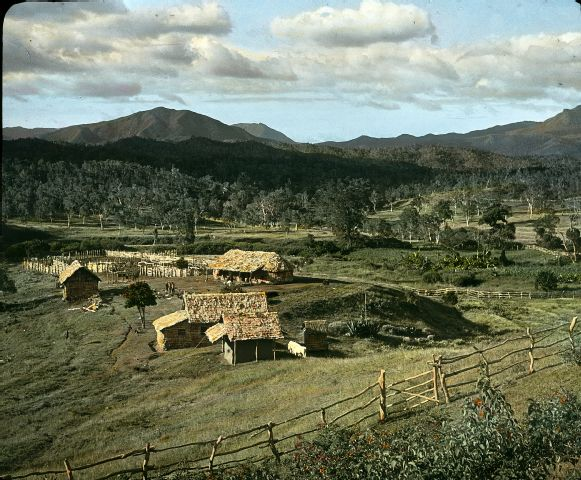
\includegraphics[width=.8\linewidth]{figures/metzdorf}
	\label{fig:metzdorf}
	\caption{Metzdorf's cattle-ranching station. CC-BY-SA Heim, \parencite{heim_farm_1921}}
\end{figure}


Philippe Dego Gohoupe (``Hao Cakeo")'s account from the 11\textsuperscript{th} November 2016 claims that Vamale speakers came from Mt. Pamale further southwest in the mountain range, and at some point moved to the valley of Tipije, whence they were chased in 1917. This is confirmed by late Galé Kalen's account from the 6\textsuperscript{th} September 2017, as well as \textcite{bensa_political_1997} and \textcite{leenhardt_figures_1978}, among others. A resettlement of the Pamale valley is unlikely in the near future, as it is considered cursed and the traditional ownership is far from clear. Some families fled to Tiendanite (confirmed by Agnès Wathea, 29.11.2017), while others chose to follow the Tipije river down to its tributary We Hava and the Pije-named coastal villages Téganpaïk, Wanaa and Tiouandé. This would explain not only the dispersion of the community, but also the languages with which they are in contact: Pije, Nemi, and Fwâi\footnote{Tiendanite and We Hava send their children to school in Fwâi-speaking Hienghène.} for Tiendanite and We Hava, Pije and Cèmuhî for the coastal villages.

The Usa variety is nowadays spoken in Tiendanite. Politically, Tiendanite is chief Goa's domain, a rival of chief Bwaarhat, whereas in 1917, Wan Kuut's chief Kavéat was an ally of both Bwaarhat and Pamale's Athea Sergent. Usa speaker Agnès Wathea mentioned that her father's clan, from Usa, was welcomed to Tiendanite by its chief, though Usa was under Athea's control, and thus not a village allied to Tiendanite. Furthermore, Vamale speakers are likely to have been on the coast prior to the war. Although the coast was disturbed by European presence, Vamale-speaking chiefs were already well in place in We Hava and Wanas by 1917 \parencite[20]{leenhardt_evenements_1978a}. Overall, this suggests a speaker mobility on an individual and family level that was relatively unimpressed by chiefs and higher politics, and followed personal alliances. This is supported by Bensa's map in \Cref{map:clan_movements}, which shows a visual representation of three oral histories, mostly pre-colonial. Regardless of this free individual networking, most family histories are tainted by the war.%, which can affect current projects, e.g. regarding research or tourist infrastructure. 

\begin{figure}[t]
% 	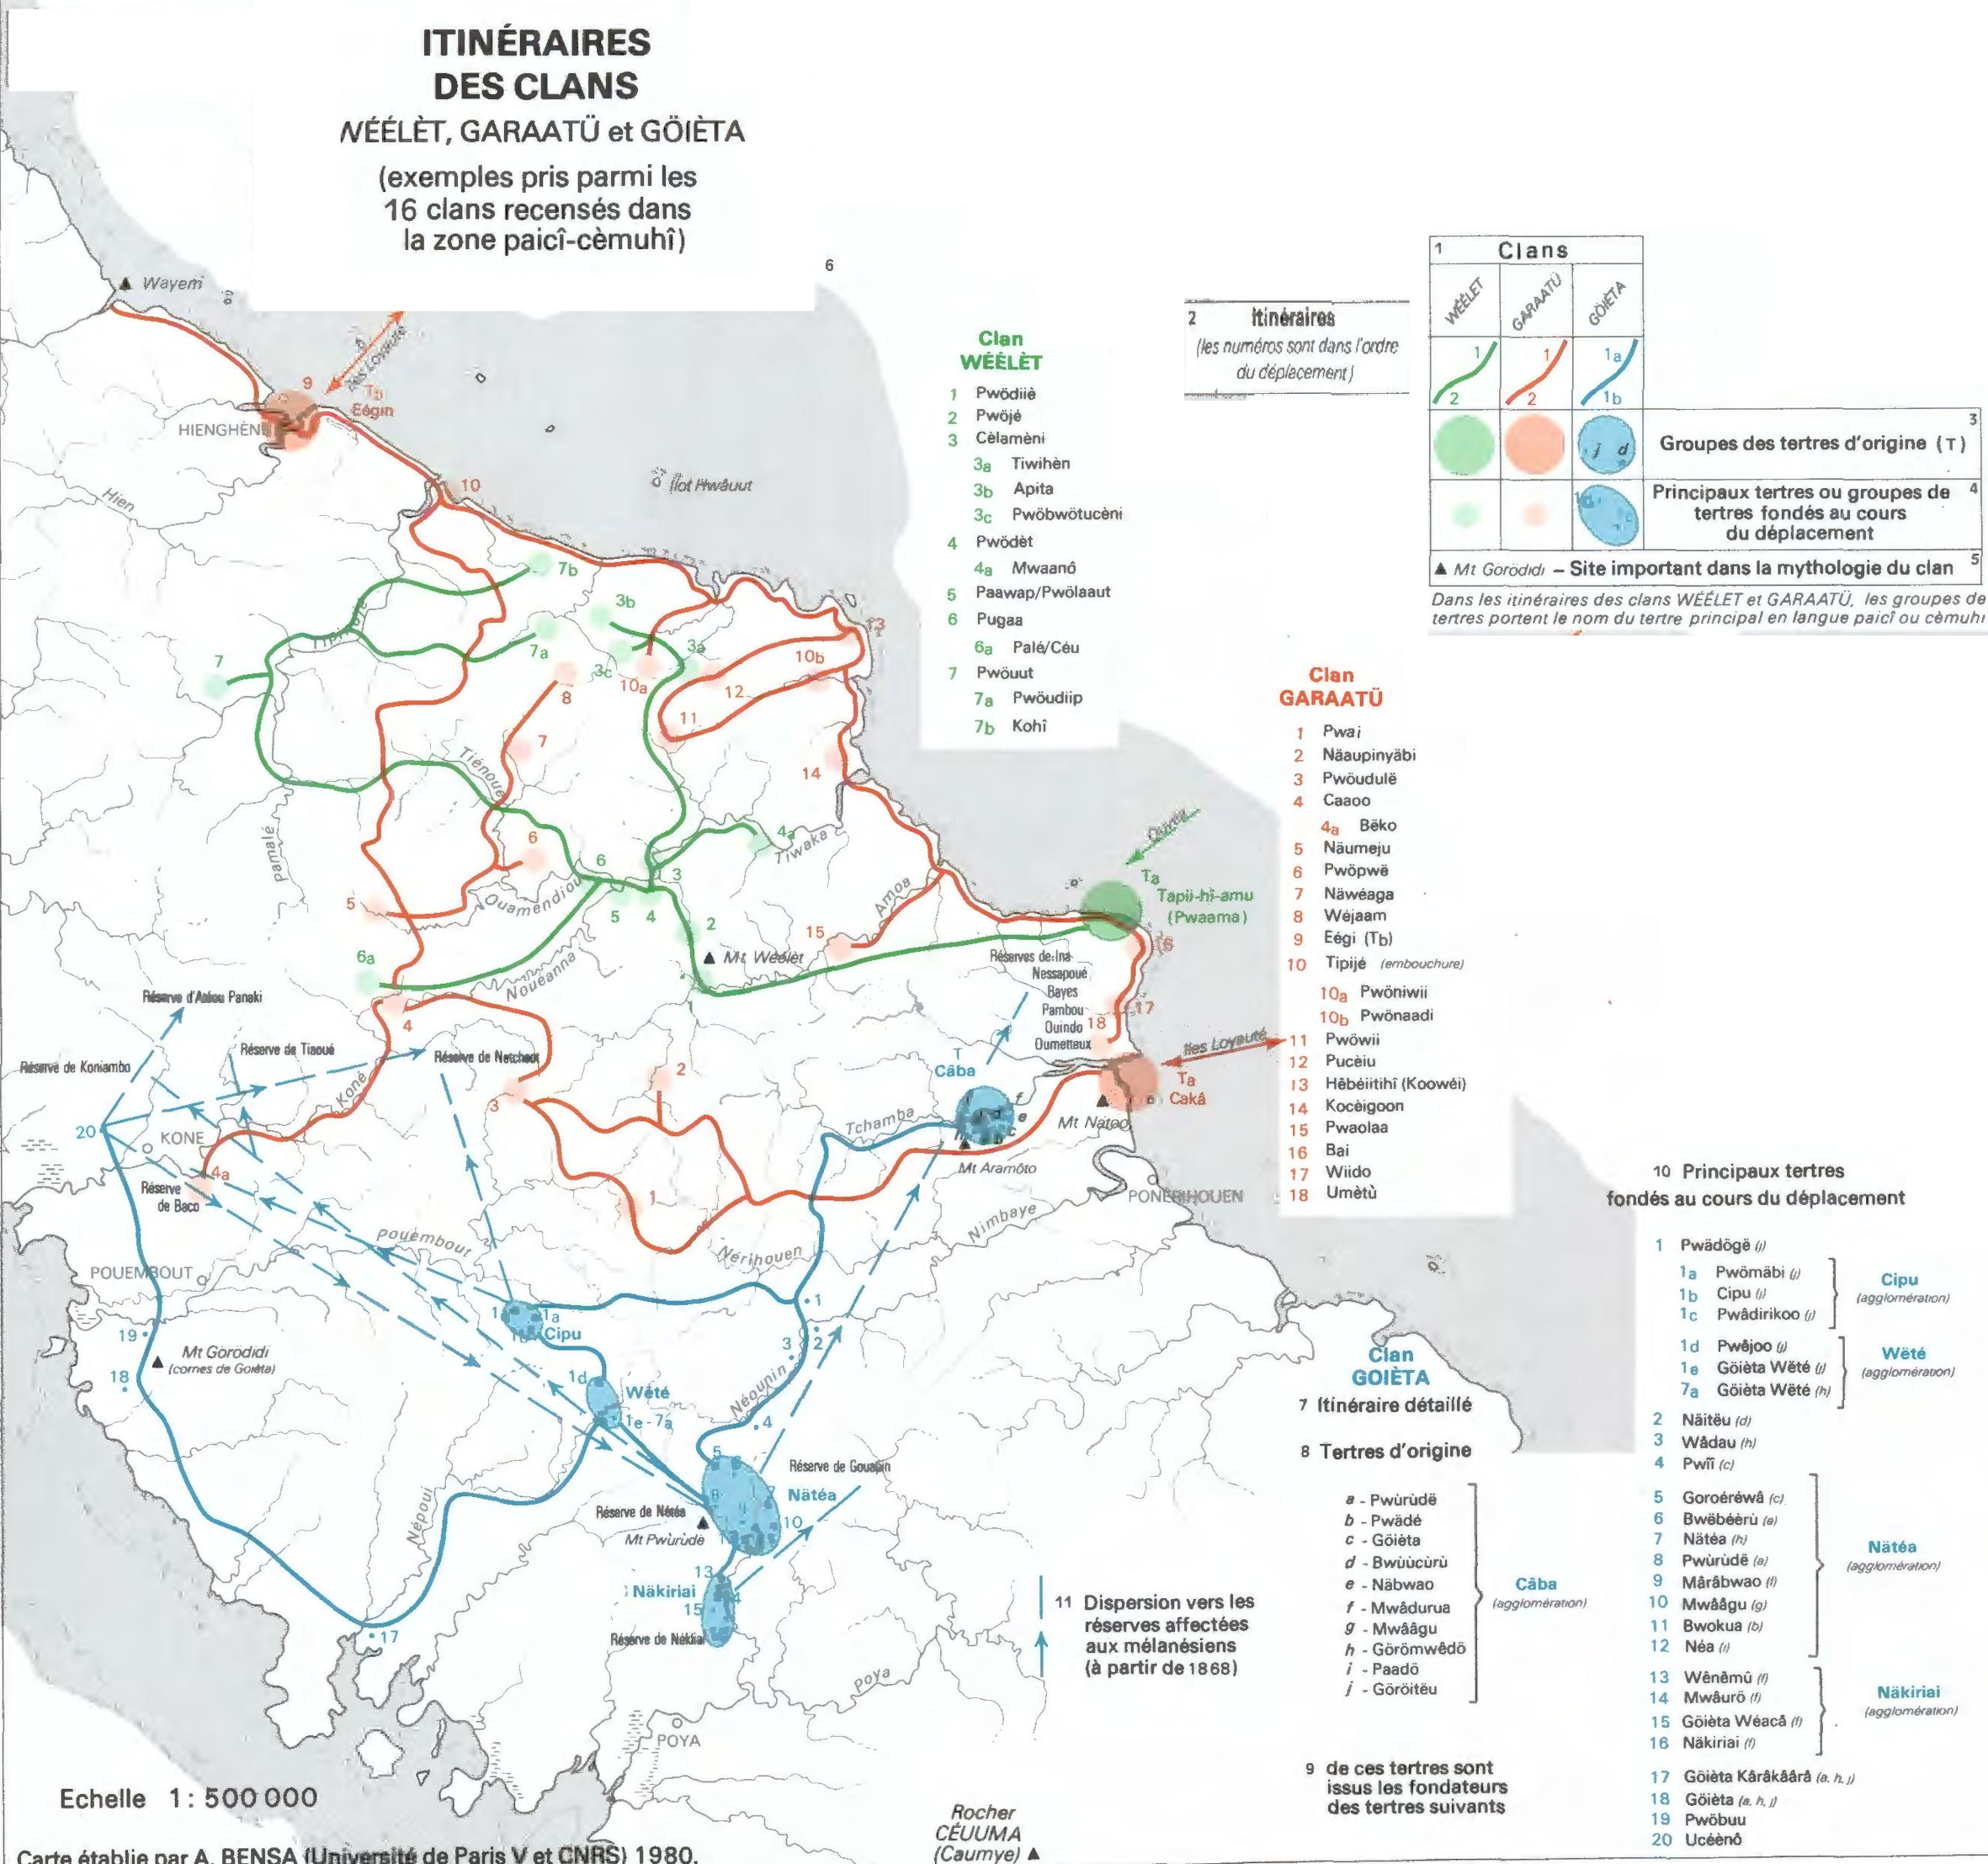
\includegraphics[width=\linewidth]{figures/clan-movements}
	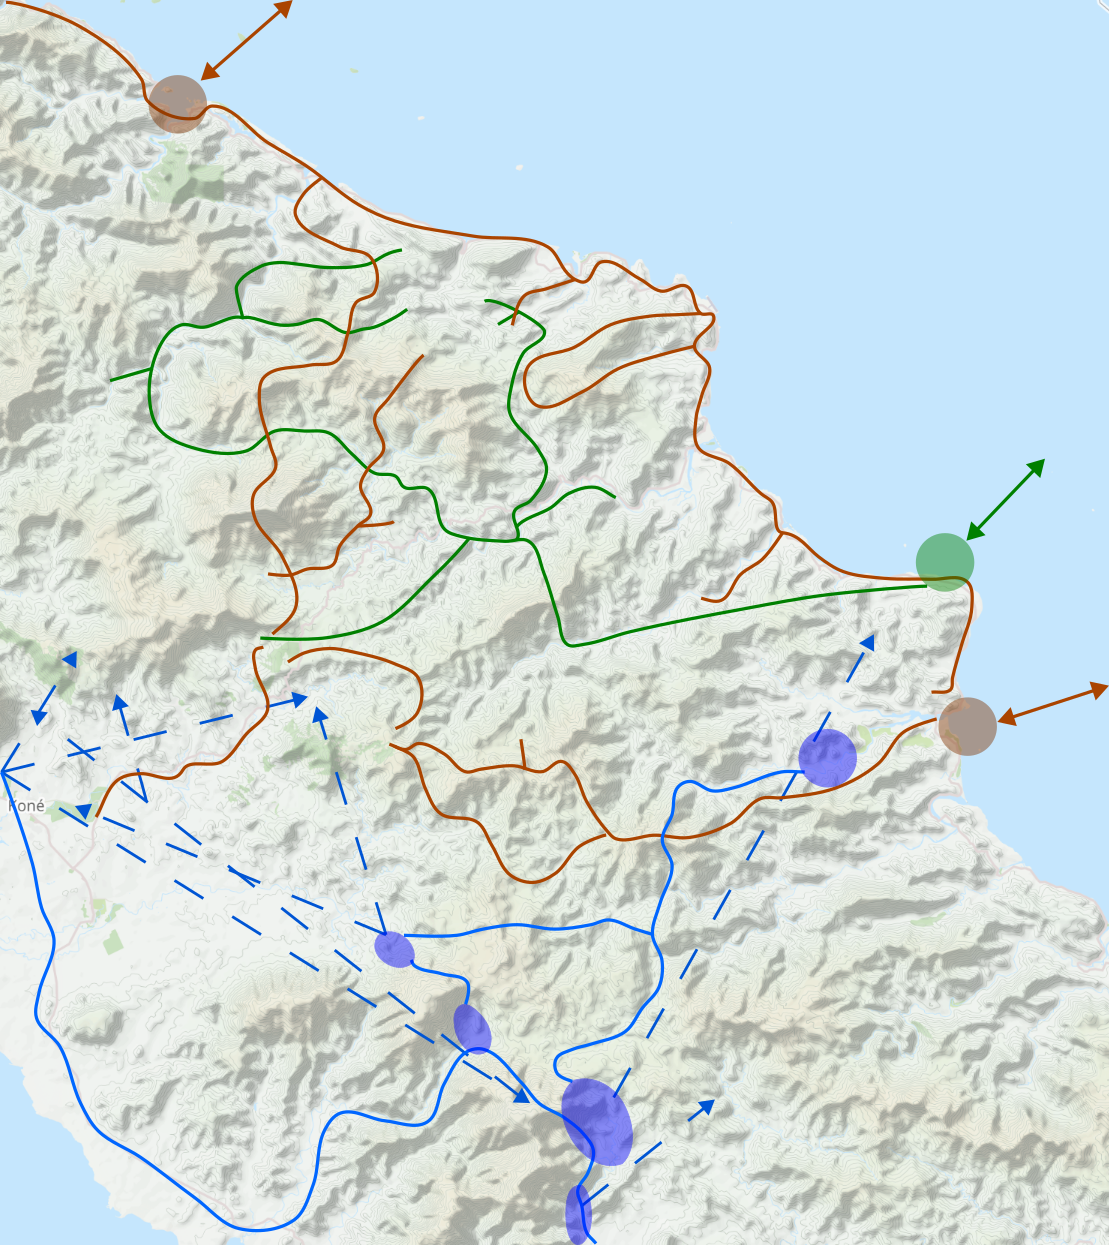
\includegraphics[width=.8\linewidth]{figures/clans.pdf}
	\caption{Map showing some clans' migrations in the Touho-Hienghène area, following \cite[71]{guiart_clans_1981}}
	\label{map:clan_movements}
\end{figure} 


\section{French policy and decline of the language}
\label{ssec:Frenchpolicy}
After the war, contact with the French and their language was sporadic until the 1950s. The colonial government locked Kanaks of diverse origins into reservations, hoping that their catastrophic demographic decline from perhaps 400,000{\interfootnotelinepenalty=10000\footnote{``To our knowledge, the only person to have proposed a density model for Grande Terre was the geographer J. P. Doumenge, who believed in a low population of about 65,000 people at contact. Nevertheless, he proposed a density of ``130 to 145 inhabitants per square kilometer of used horticultural surface'' (\citealt[463]{doumenge_terroir_1982}, original text in French). Reducing his figures by half (i.e., seventy p/km\textsuperscript{2}) to account for the vague status of the phrase \qu*{used horticultural surfaces}, and again using only one-third of the surface of the island, we would arrive at 400,000 people." \parencite[316]{sand_what_2007}}} people before contact \parencite[316]{sand_what_2007} to just about 27,000 in the early 1920s \parencite[309]{sand_what_2007} would in time lead to a total disappearance in contact with a ``superior race" \parencites[289]{stern_colonies_1943}[2]{salaun_francophonie_2005}. French colonial language policy was not very invasive and concentrated on prohibiting the use of indigenous languages in public\footnote{The ``public" being defined by the presence of settlers.} \parencite[2]{salaun_francophonie_2005}. However, most Kanaks were confined to reservations \parencite[3]{demmer_nationalisme_2003} in which the only outsiders were missionaries and \textit{gendarmes}, so even that policy did not affect many people. %hence little influence

The event truly leading to speaker decline was schooling, which only began on any scale to speak of in the 1950s.\footnote{Note that Leendhardt counted only around 50 speakers in the 1940s, but schooling prevented a subsequent language transmission, and therefore a quicker recovery.} Before that, Kanaks were not citizens,\footnote{The \textit{Code de l'Indigénat} specifying this was abolished in 1946, but this was not noticeably implemented until 1952.} and the only schooling was privately done by the churches. Most elders in the villages do not enjoy speaking French and are multilingual in Kanak languages. Until the 1980s, the Vamale-speaking area was untouched by public schooling. Most children went to the Protestant private school in Tiouandé (\textit{Fédération de l'enseignement libre protestant}, F.E.L.P., closed in the 1980s) or to Catholic institutions like the one in Tuo Mission. Nowadays, all children go to the public schools in Hienghène (for Oué Hava) and Touho (for Tiouandé and Téganpaik), where the dominant Kanak languages are Fwâi and Cèmuhî respectively. TV, radio, the spread of smartphones and the advent of mobile internet in early 2019 have added to language contact. 

%Having touched upon the history of Vamale as known by European sources, and complemented by Kanak oral sources, the present situation is described below, first in terms of human geography.

% \section{Modern context}



\chapter{Phonology}
\label{ChapterPhon}
	
There are 55 phonemes; 20 phonemic vowels (5 qualities, length and nasality are contrastive) and 35 consonants. The number of both consonant and vowel phonemes puts the phoneme inventory of Vamale in the top 10\% on Phoible (with ca. 3000 compared inventories) \parencite{phoible}, and in the second-largest group of the sample studied by Maddieson et. al in \citetitle{wals}, which assigns it a high consonant-to-vowel quality ratio.\footnote{Note that this counts vowel qualities but not contrastive quantity, hence 35 consonants\slash 5 vowels  yielding a ratio of 7.}
The emphasis on consonants is typical of the Northern and Far Northern languages, and was not diminished by the proximity of consonant-poorer Cèmuhî, nor was it substantially enriched by Pije, which has e.g. /ɾ̥/.
	
	
\section{Transcription}
\is{Transcription}
Following the transcription system established by \textcite{ozanne-rivierre_phonologie_1982}% (\textbf{Could you say whether this system is rather broad or narrow, i.e. rather phonemic or phonetic? Your pre-nasalized segments in this paragraph and Table 1.1 suggest the latter...})
, this work will use \ort{h} after plosives to mark aspiration (regardless of its phonemic status), \ort{h} before nasals and liquids to mark voicelessness, and the circumflex diacritic to mark nasal quality in vowels (see \Cref{tab:transcr_system} for an overview). All voiced plosives are typically pre-nasalized%, a feature inherited from Proto-Oceanic
: /ᵐb/, /ⁿd/, /ⁿɟ/, /ᵑg/. This is systematic and, following the local linguistic tradition, will not be represented. Vowels are nasalized after nasals, and often also before them (this includes the pre-nasal elements in voiced plosives such as /ᵐb/, to an extent). There is also interplay with aspirated plosives for historical reasons  (see \sectref{ssec:Aspiration}). Only phonemically nasal vowels will be represented as nasal, with the circumflex diacritic \ort{\^{}} used in all Northern transcription systems. Compare the representations of (\ref{ex:nasal}) with phonemic nasalization with (\ref{ex:nasal2}) with predictable aspiration.
	\is{Vowels!Nasal vowels}
	
	
	\ea \label{ex:nasal}
		[wĩ̃ːn jeː]\\
		\gll wîî-n yee\\
		 strength-\gl{nspec}.\gl{poss} tree\\
		\glt \qu{strength of a tree}
		\z
		
		
		\ea \label{ex:nasal2}
		[wĩːn jeː]\\
		\gll wii-n yee\\
		 field-\gl{nspec}.\gl{poss} tree\\
		\glt \qu{orchard}
	\z  



True minimal pairs between oral and phonemic nasal vowels are rare, while contexts in which phonemically oral vowels are nasalized abound. The degree of nasality depends on the speaker, so the phonetic difference depicted in example (\ref{ex:nasal}) is not a representative or reliable criterion to identify phonemically nasal vowels, though the latter tend to be more strongly nasal than nasalized ones. %Since phonemic status is not always clearly determined, circumflex diacritics will also mark nasal vowels where the nasal quality is not necessarily phonologically conditioned, as for \ort{phwê} /pʰʷɛ̃/ \qu{moon} (see \sectref{ssec:Aspiration} and \sectref{ssec:NasalV}).
	
%	\begin{table}
%		
%		\centering
%		\caption{Transliteration system used in this thesis}
%		\label{tab:transcr_system}
%		\begin{tabular}{l|llllllllllllllllll}
%		Aspirated Plosives&  \ort{phw}& /pʰʷ/& \ort{ph} & /pʰ/ & 	\ort{th}& /tʰ/& \ort{ch}&[cʰ]&\ort{kh}&/kʰ/&&&&&&&& \\
%		Tenuis Plosives& \ort{p} & /p/ & \ort{t}& /t/ & \ort{c} & /c/ & \ort{k} & /k/ &&&&&&&&&&\\
%		Voiced Plosives& \ort{b}& /ᵐb/&\ort{bw}& /ᵐbʷ/& \ort{j}& /ⁿɟ/ & \ort{g} & /ᵑɡ/ &&&&&&&&&&\\
%		
%		Nasals& \ort{m} /m/ &  \ort{hm}& /m̥/& \ort{n} & /n/ & \ort{hn} & /n̥/ &\ort{ny}& /ɲ/& \ort{hny}& /ɲ̊/ & \ort{ng} & /ŋ/ &  \ort{hng} & /ŋ̊/ &&&\\
%		Fricatives & \ort{f}  /f/ & \ort{fw}  /fʷ/ & \ort{v}  /v/ & vw & /vʷ/ & \ort{s}& /s/&	\ort{xh}& /x/&	\ort{x} & /ɣ/ & xw & /xʷ/ & \ort{h} & /h/ &&&\\
%		Approximants & \ort{l}  /l/ & \ort{hl} & /l̥/ & \ort{w} & /w/ & \ort{y} & /j/ & \ort{hy}& [ç] \goodtilde [j̥]&&&&&&&&&\\
%		Vowels&	\ort{i}  /i/ &	\ort{ii}& /iː/ & \ort{î}& /ĩ/ & \ort{îî} & /ĩː/&\ort{e}&[e] \goodtilde [ɛ] & \ort{ê} & /ɛ̃/&\ort{o}& [o] \goodtilde [ɔ]&\ort{ô} & /ɔ̃/&&&\\
%	
%		\end{tabular}
%	\end{table}

	\begin{table}
	\caption{Transliteration system used in this book}
	\label{tab:transcr_system}

	\begin{tabular}{llllll}
	\lsptoprule
		  \ort{ph} /pʰ/ &  \ort{phw} /pʰʷ/&	\ort{th} /tʰ/& \ort{ch} [cʰ]&\ort{kh} /kʰ/ \\
		\ort{p}  /p/ &\ort{pw}  /pʷ/& \ort{t} /t/ & \ort{c}  /c/ & \ort{k}  /k/ \\
		\ort{b} /ᵐb/&\ort{bw} /ᵐbʷ/& \ort{d} /ⁿd/&\ort{j} /ⁿɟ/ & \ort{g}  /ᵑɡ/ &\\
		  \ort{hm} /m̥/& \ort{hmw} /m̥ʷ/& \ort{hn}  /n̥/ & \ort{hny} /ɲ̊/ &   \ort{hng}  /ŋ̊/ \\
	\ort{m} /m/&	\ort{mw} /mʷ/ & \ort{n}  /n/ &  \ort{ny} /ɲ/& \ort{ng} /ŋ/ \\
		\midrule
		 \ort{f}  /f/ & \ort{fw}  /fʷ/ & \ort{s} /s/&	\ort{xh} /x/& \ort{xw}  /xʷ/ & \ort{h}  /h/ \\
		  \ort{v} /v/ & \ort{vw}  /vʷ/ &&	\ort{x}  /ɣ/&& \\
&&	\ort{l}  /l/ & \ort{y}  /j/ & \ort{w}  /w/ &\\
&&	\ort{hl}  /l̥/ & \multicolumn{2}{l}{\ort{hy} [ç] \goodtilde [j̥]}&\\
	\midrule
	\ort{i}  /i/ &&	\ort{ii} /iː/ &&&\\
	 \ort{î} /ĩ/ && \ort{îî}  /ĩː/&&&\\
	 \ort{e} [e] \goodtilde [ɛ] &\ort{ee} [eː] \goodtilde [ɛː] &&&\\
	  \ort{ê} /ɛ̃/&&\ort{êê}  /ɛ̃ː/&&&\\
	  \ort{o} [o] \goodtilde [ɔ]&\ort{oo} [oː] \goodtilde [ɔː]&&&\\
	  \ort{ô}  /ɔ̃/&&\ort{ôô}  /ɔ̃ː/&&&\\
		\lspbottomrule
	\end{tabular}
\end{table}


	\begin{sloppypar}
	Vamale speakers frequently code-switch to French. Established loanwords such as \textit{watuut} \qu{car} are transcribed according to the system in \Cref{tab:transcr_system}, whereas \textit{ad hoc} loans are written as they would be in French and italicized to help distinguish them from older Vamale words (\ref{ex:devoirs}).
	\end{sloppypar}
	
	\ea \label{ex:devoirs}
		\gll tha le=vwa \textit{devoirs}-le\\
			  \gl{ass} 3\gl{pl}=do homework-3\gl{pl}.\gl{poss}\\
		\glt \qu{They do their homework.}
	\z\index[gls]{ass}
	
	\section{Consonants}
	\label{sec:consphonemes}
	\is{Consonants}
	The consonants, shown in \Cref{tab:cons}, can be classified along two axes: aspiration (aspirated vs. non-aspirated) and nasality (nasal vs. semi-nasal vs. oral). This has historical reasons, as will be shown in \sectref{sec:phonhist_dev}. 
	While all consonants may appear word-initially and between vowels, a historical neutralization has reduced the set of syllable-final ones: /p, t, tɕ, k, m, n, ɲ, ŋ/, i.e. simple voiced nasals and voiceless plosives. Syllable-final /k/, /tɕ/ and /ɲ/ are much rarer than the others and are undergoing mergers with /ʔ/, /t/, and /n/ respectively. 
	\begin{itemize}
		
	\item /piuk/ \qu{spark} $\rightarrow$ [ˈpiˑ.uʔ] 
	\item /jilowec/ \qu{tree sp.} $\rightarrow$  [ⁿɟi.ˈlo.wɛt] 
	\item /waɲ/ \qu{consequence of taboo breaking} $\rightarrow$ [wan])

\end{itemize}
	 /k/ and /tɕ/ are often simply dropped. The deletion of final consonants is a sound change that is described as affecting mountain Voh-Koné varieties \parencite[25]{campbell_phenomenon_1987}, and is furthest advanced in the coastal variety of Vamale. This final consonant deletion only concerns inherited lexemes, since numerous loanwords from French and Kanak languages feature other syllable-final consonants (\textit{bagaas} \qu{luggage}, \textit{cakes} \qu{\gl{expl}}).
	While syllable-final /k/ is often dropped, /k/ is also rare in syllable onsets: many words with k- are either loans or grammatical terms, e.g. \textit{ka} \qu{\gl{sbj}}, \textit{ka} \qu{\gl{cnj}}, \textit{ko} \qu{obl}, \textit{-ke} \qu{\gl{tr}}, \textit{kai} \qu{who?}, \textit{kacahô} \qu{rather than}, \textit{kavi} \qu{but}. Lexical, apparently non-borrowed words number fewer than 10 items in the recorded dictionary. While a historical sound change lenited *k- to ɣ- (see \sectref{sec:quesphon}), explaining the rarity of \textit{k}-, it is noteworthy that many words that retained initial k- are grammatical terms.
	
	Vamale consonants distinguish a voiceless series from a pre-nasalized voiced series. This is a feature retained from Proto-Oceanic, and not widespread east of New Caledonia \parencite[196--197]{ozanne-rivierre_proto-oceanic_1992}. A typical feature of Northern New Caledonian is the presence of labio-velar plosives and fricatives, and voiceless nasals and liquids. Labio-velarized consonants do not precede /u/ and /o/ for historical reasons: one element merged into the other.

	\begin{table}
		\caption{Consonants in Vamale. Non-phonemes are in brackets.}
		\begin{tabular}{ *6{l} }
			\lsptoprule
			             & Bilabial & Lab. Bilab. & Labiod. & Lab. Labiod. \\\midrule
			Plosive      & pʰ p ᵐb & (pʰʷ) pʷ ᵐbʷ &         &              \\
			Nasal        & m̥ m     & m̥ʷ mʷ        &         &            \\
			Tap          &         &              &         &              \\
			Fricative    &         &              & f v     & fʷ vʷ        \\
			Approximant  &         &              &         &              \\
			Lat. Approx. &         &              &         &              \\\midrule
			             & Alveolar & Palatal & Velar & Lab. Velar & Glott. \\\midrule
             Plosive     & tʰ t ⁿd & (cʰ) c ⁿɟ & kʰ k ᵑɡ  &    &  \\
             Nasal       & n̥ n     & ɲ̊ ɲ       & (ŋ̊) ŋ    &    &  \\
             Tap         & (ɾ)     &           &          &    &  \\
             Fricative   & s       &           & x ɣ      & xʷ & h \\
             Approximant &         & j         &          & w  &  \\
             Lat. Approx.& l l̥     &           &          &    &\\
			\lspbottomrule
		\end{tabular}
		\label{tab:cons}
	\end{table}

	\subsection{Examples}
	A table listing examples in word-initial, -internal, and -final positions is given in \Cref{tab:consex}. No study was done on the frequency of the phonemes, but some consonants are much rarer than others. Syllable-final /k/ has all but disappeared in a regular sound-change, and occurs only in loans from Pije and other languages: e.g. \textit{piuk} \qu{nail}\footnote{POc *pituqun, \textit{piguk} \qu{star} in Nêlêmwa \parencite[21]{bril_nelemwa_2002}.} and \textit{xhwahyuk} \qu{whistle} are originally Pije. %It is noteworthy that Campbell described this apocope as even more complete for Vamale, with \textit{piu} \qu{star} (normally \textit{xhafuthiin} in coastal Vamale, but \textit{daan-piuk} \qu{thorn-spark; nail}) \parencite[120]{campbell_phenomenon_1987}. 
%	Syllable-final /c/ is similarly on its way out, and final /ɲ/, lacking contrastive contexts, seems to merge with /n/. 
	/r/ only occurs in loans. Initial /ŋ/ is probably a loan phone from Pije, given that it only appears in one plant species name (\textit{ngeein}), and is in free variation with \textit{mwangin} \goodtilde \textit{ngangin} \qu{sour}. Finally, all aspirated plosives except /tʰ/ are rare.
	
	\begin{table}
		\caption{Examples showing Vamale consonants in monomorphemic words.}
	\small
	\resizebox{.85\textwidth}{!}{
		\begin{tabular}{l *3{l@{~}l} }
			\lsptoprule
			& \multicolumn{2}{l}{Initial} & \multicolumn{2}{l}{Medial} & \multicolumn{2}{l}{Final}\\\midrule
			\multicolumn{7}{l}{Plosives}  \\
			&   \textit{pwan}& \qu{on} & \textit{sapwen}& \qu{clothing} &&\\
			&	\textit{phwaat}& \qu{clear} & \textit{xhwaaphwê}& \qu{araucaria sp.} & &\\
			&	\textit{bwan}& \qu{head} & \textit{siibwi}& \qu{rat} & & \\
			&	\textit{pa}& \qu{\gl{prf}} & \textit{ape}-& \qu{trace} & \textit{thap}& \qu{pandanus} \\
			&	\textit{phuake}& \qu{prod} &  &&&\\
			&	\textit{ba}& \qu{wall} & \textit{abu}& \qu{1\gl{du}.\gl{excl}} & &\\
			&	\textit{thake} & \qu{throw} &  \textit{mathila}& \qu{bird sp}& &\\
			&	\textit{ta}& \qu{go up} & \textit{mata}& \qu{sing} & \textit{fuut}& \qu{whistle} \\
			&	\textit{da}& \qu{spear} & \textit{udu}& \qu{drink} & &\\
			&	\textit{cabi}& \qu{break} & \textit{kicaa}& \qu{jealous} & \textit{tuuc}& \qu{take out} \\
			&	\textit{jigo}& \qu{mangrove} & \textit{vije}& \qu{bird snare} & & \\
			&	\textit{ka}& \qu{\gl{sbj}} & \textit{buke}& \qu{flower} & \textit{piuk}& \qu{spark} \\
			&	\textit{gi}& \qu{adze} & \textit{hagu}& \qu{snake} & &\\
			\midrule
			\multicolumn{7}{l}{Fricatives, glides, and liquids} \\
			&   \textit{fuu}& \qu{wash} & \textit{fufudo} & \qu{foam} &&\\
			&	\textit{vaa}& \qu{war} & \textit{fava}& \qu{four}&&\\
			&	\textit{fwa}& \qu{hole} &  \textit{waafwap}& \qu{raven} && \\
			&	\textit{vwa}& \qu{do, have} & \textit{xhaavwa}& \qu{wait} & &\\
			&	\textit{siteke}& \qu{sacred} & \textit{gase}& \qu{1\gl{pl}.\gl{incl}} &&\\
			&	\textit{xhopwen}& \qu{big} & \textit{haxhi}& \qu{forgive} && \\
			&	\textit{xhwatin}& \qu{small} & \textit{sixhwe}& \qu{imitate} & & \\
			&	\textit{holeeke}& \qu{thank} & \textit{yahan}& \qu{leave} &&\\	
			&	\textit{xat}& \qu{sun} && && \\
			&	\textit{xhat} & \qu{clitoris} & \textit{bwaxhu}&\qu{hat} &&\\
			&	\textit{yatan}& \qu{name} & \textit{vaya}& \qu{work} & &\\
			&	\textit{wadan}& \qu{time} &   \textit{nyawan}& \qu{spirit} &&\\
			&	\textit{ra}-& \qu{\gl{reccont}} & \textit{gere}& \qu{fat} & &\\
			&	\textit{lu}& \qu{3\gl{du}} &\textit{pwalalu}& \qu{rainbow} & &\\
			&	\textit{hluupwi}& \qu{suck in} &\textit{bwahli}& \qu{long} & &\\
			\midrule	
			\multicolumn{7}{l}{Nasals} \\
			&	\textit{hmwet}& \qu{tired} & \textit{saahmwa}& \qu{banana} & &\\
			&	\textit{mwa}& \qu{house} & \textit{imwi}& \qu{grab}& & \\
			&	\textit{hma}& \qu{arrive} & \textit{cahma}& \qu{whereas} & & \\
			&	\textit{ma}& \qu{\gl{com}} & \textit{cama}& \qu{if} & \textit{xam}& \qu{mat}\\
			&	\textit{hnep}& \qu{sail} & \textit{ehni}& \qu{prox}& & \\
			&	\textit{naen}& \qu{now} & \textit{jinu}& \qu{power} & \textit{thiin} & \qu{close} \\
			&	\textit{hnyimake}& \qu{think} & \textit{bwihnyo} &\qu{clam}  & & \\
			&	\textit{nyau}& \qu{bad} & \textit{xhanyip}& \qu{dream} & \textit{wany}& \qu{punishment}\\
			&	\textit{ngein}& \qu{cycas sp.} & \textit{dingan}& \qu{creek} & \textit{vaang}& \qu{unknown} \\
		\lspbottomrule
		\end{tabular}
		}
		\label{tab:consex}
	\end{table}
	
%	\footnotetext{\gl{prf} }
	\subsection{Marginal phonemes}
	\label{sec:quesphon}
	
	\is{Marginal phonemes![ŋ̊]}
	Some segments appear rarely, are not produced by all speakers, or present a distribution which hints at (former) allophony. This affects most voiceless plosives, the tap \ort{r} [ɾ], the voiceless lateral approximant [l̥] and the voiceless velar nasal. \ort{hng} /ŋ̊/ only appears in \textit{jahngan} \qu{length}, and is in free variation with its voiced counterpart. Three factors indicate that /ŋ̊/ is a loan in this word: (a) the aspiration of nasals can be almost or completely inaudible (intervocalic nasals are more audibly aspirated than initial ones), (b) neither Bwatoo nor Hmwaveke seem to have it in any other words, and (c) only Western Nemi (no present-day contact) has it as a phoneme. 
	
	\is{Marginal phonemes![ɾ]}
	The tap \ort{r} [ɾ] is a phoneme in Nemi and in Fwâi \parencite[18; 19]{ozanne-rivierre_phonologie_1982}. It appears only in loanwords in Pije \parencite[17]{ozanne-rivierre_phonologie_1982} and Cèmuhî \parencite[21]{rivierre_langue_1980}, and does the same in Vamale. There is one instance where I recorded \ort{ra-} as an aspectual prefix \qu{to have been doing for a short while} in unelicited speech. I was able to contrast it with \ort{xa-} /ɣa/, compare examples \REF{ex:x} and \REF{ex:r}.
	
	\ea
	\label{ex:x}
		\gll a=xa-soom la\\	
	 3\gl{sg}=\gl{agt}.\gl{nmlz}-swim be.here\\
	\glt \qu{S/he usually swims here.}
	\z
	
	
	\ea\label{ex:r}
	\gll a=ra-xa-soom la\\
	 3\gl{sg}=\gl{reccont}-\gl{agt}.\gl{nmlz}-swim be.here\\	
	\glt \qu{S/he recently picked up the habit of swimming here.}
		\z
	
	\ort{ra-} is described for Bwatoo as a continuative particle, see example \REF{ex:Bwatoo_ra} \parencite[57]{rivierre_bwatoo_2006}, whereas \ort{xha} /xa/ is the habitual aspect marker (/ɣa-/ in Vamale). \textit{Ra} is not used in these contexts in Vamale (where the continuative marker is \textit{balan}). \textit{Ra} is probably a loan from the West Coast, and [ɾ] most likely a relatively free variant of /ɣ/, except in this one prefix \textit{ra-} \qu{\gl{reccont}}.
	
	\ea \label{ex:Bwatoo_ra}	
	\gll ka le ra vila na ni bee-le\\
	 \gl{cnj} 3\gl{pl} \textit{persist}. dance \gl{agt} \gl{def}.\gl{pl} peer-3\gl{pl}.\gl{poss}\\
	\glt \qu{The others keep dancing.}
	\z
	
	
	\ea	
	\gll a bwaa ra Numea\\	
	 3\gl{sg} \gl{ipfv} \textit{persist}. N.\\
		\glt \qu{S/he is still in Noumea.}	
	\z
	
	\is{Marginal phonemes![kʰ]}
The status of [kʰ] is tricky in the sense that, while both the aspirated and the non-aspirated phone exist, the aspirated one only very rarely occurs without a nasalized vowel following it. There are no minimal pairs with [k], and the few occurrences of [kʰ] before oral vowels are loanwords or due to fortis-spreading (see \sectref{ssec:Aspiration}). 

	\is{Marginal phonemes![pʰ]}
Bilabial voiceless plosives exist with aspiration and without, as well as with labiovelarization. So far, the origin of either remains to be established, as the regular sound changes reconstructed by \citeauthor{ozanne-rivierre_structural_1995} mostly led to the development of fricatives. [pʰ] is attested before the oral rounded vowels [u] and [o], and before nasal vowels. The latter are a sound class intimately related to aspiration, as is discussed in \sectref{ssec:Aspiration}. Most instances of [pʰ] before a nasal vowel may be produced with a velar fricative [pʰʷ] \goodtilde [pχ]. The glide [w] and rounded back vowels have merged in modern Vamale. There are no minimal pairs between [pʰ] and [pʰʷ]. There are no perfect minimal pairs with either and /p/, though this contrast is clearer, e.g. neither /p/ nor /pʷ/ precedes nasal vowels. Both /p/ and [pʰ] before oral back vowels are rare. The following words constitute the entirety of the types recorded in the lexicon, many of which are found in non-Voh-Koné languages as well: \begin{itemize}
\item \textit{pu} \qu{on the ground} \item \textit{puput} \qu{behind sth inanimate} \item \textit{phuake} \qu{wiggle} \item  \textit{poon} \qu{coconut fibre} \item \textit{phoop} \qu{snail}, \textit{phom} \qu{butterfly} \item \textit{pola} \qu{type of weaving} \item \textit{photha} \qu{sexual taboo; women's part of the village}\footnote{From \citegen{leenhardt_langues_1946} notes, not used nowadays.} 
\end{itemize}
Furthermore, there are no instances of /f/ and /fʷ/ followed by a nasal vowel, but many cases of /f/ before rounded back vowels. Hence, an imperfect distribution of labiodental fricatives and bilabial aspirated plosives can be identified: front and central vowels are only found after fricatives, nasal vowels only after plosives, and rounded back vowels can follow either. In conclusion, [pʰ] and [pʰʷ] may be former allophones of /f/ and /fʷ/ before nasal vowels, and [pʰ] is now present before oral vowels due to contact with other languages, perhaps Pije \parencite[518]{rivierre_contact_1994}. The unaspirated bilabial plosives were borrowed from neighboring languages as well \parencite[516]{rivierre_contact_1994}, or constitute remains of an incomplete sound change *p $\rightarrow$ \textit{v}. 
 %\todo{where is p and pw from?}
	%BUT: pu/puput, poon/pola/pook (loanwords?), pwa, etc. fuu, foovwat etc. 
	
	%xxFor these reasons, both [pʰ] and [kʰ] are old allophones of /p/ and /k/ in old Vamale words, and nowadays available loan phones in loanwords. 
	
	\subsection{Labio-velarized consonants}
	\is{Consonants!Labio-velarized consonants}
	Labio-velar consonants in Vamale are all labial (/ᵐbʷ/, /fʷ/, /mʷ/, etc), with the exception of /xʷ/. To explain this, Campbell suggests that /xʷ/ should be analyzed as an allophone or a surface realization of /w̥/ \parencite[37]{campbell_phenomenon_1987}, with /w̥/ as the fortis %couterpart to 
	/w/ (see \sectref{ssec:Aspiration} for an introduction to Vamale fortis). This makes sense as it makes the Hmwa(v)eke systems fit into their regional context, as voiceless liquids and glides are widespread in other Northern languages. 
		%\subsection{Pre-nasalized consonants}
	%Pre-nasals have bled into Kanak French, seems to intensify when people want to emphasize their Kanakdom.
	%Because a nasal followed by a voiced plosive at the same point of articulation ([nd],[mb],[nɟ],[ŋg]) could be viewed as a part of the plosive, there are no morpheme-final voiced plosives, except in loan words.
	
	\subsection{Voiceless nasals}
	\label{sec:phonhist_dev}
	\is{Consonants!Voiceless nasals}
	Every nasal except /ŋ/ has a fortis, i.e. voiceless counterpart, e.g. /m̥uːn/ \qu{smoke} vs /muːn/ \qu{blossom}. Like most of the aspirated plosives, voiceless nasals in Vamale have probably developed from forms that were reduplicated in POc and geminated in PNC, and which were perhaps already devoiced in Proto-North, for instance *nana(q) \qu{pus} $\rightarrow$	\textit{hnau-}\slash\textit{hnau-} \qu{snot} \parencite[27]{ozanne-rivierre_phonologie_1982}.

	In Bwatoo and in Vamale, the phonation of nasals and liquids can be influenced by the fortis status of other consonants in the surrounding syllables. Bwatoo examples include the following, with the triggering consonants in bold:
	
	\ea  \parencite[27]{rivierre_bwatoo_2006}
		\ea \textit{\textbf{f}omwa} \goodtilde \textit{\textbf{f}ohmwa} \qu{village}
		\ex \textit{\textbf{xh}oomu} \goodtilde \textit{\textbf{xh}oohmu} \qu{old}
		\ex \textit{\textbf{xh}uni} \goodtilde \textit{\textbf{xh}uhni} \qu{spear sling}
		\ex \textit{\textbf{xhw}aloop} \goodtilde \textit{\textbf{xhw}ahloop} \qu{be on the belly}
		\z
	\z
		
	Even though voiceless nasals have a different historical development from voiced nasals, and though they contrast in some minimal pairs, this account is unsure of how to describe them phonetically. The nasal in \ort{hnau-} might be voiceless [n̥], pre-aspirated [hn], or both, and it is unclear as of yet which of the allophones is the underlying form. The aspiration, even though it often starts before the nasal is articulated, does not seem to stop before the beginning of the nasal's production (the result is thus closer to [hn̥ãw̃]).
	
	\subsection{Aspiration} \label{ssec:Aspiration}
	\is{Consonants!Aspiration}

In Vamale, aspirated plosives were for the most part borrowed from neighboring languages, except for /tʰ/. For reasons explored below, voiceless nasals and liquids, and aspirated plosives influence each other and have a similar history. \Cref{tab:asp_dist} summarizes the distribution of aspirated consonants and nasal vowels, which also correlate, for reasons explored below.
Aspiration is widespread in North New Caledonian languages, with the exception of tonal Cèmuhî and Paicî. Aspirated plosives developed from geminates, as did voiceless nasals:
\begin{itemize}
\item POc CV.CV reduplication is reduced to geminate CCV, and then to: \begin{itemize}
	\item Cʰ in the non-tonal northern languages \parencite[27]{ozanne-rivierre_phonologie_1982}, then ultimately fricatives in Vamale
	\item CV́ in Cèmuhî and Paicî \parencite[203]{ozanne-rivierre_proto-oceanic_1992}.
\end{itemize}
\end{itemize}

In Vamale, however, this only led to aspirated word-initial plosives in the case of /tʰ/: *t̪t̪, *cc $\rightarrow$ /tʰ/ \parencite[513]{rivierre_contact_1994}, which also explains the presence of minimal pairs contrasting nasal and oral vowels after /tʰ/ (e.g. \textit{tha} \qu{\gl{ass}}; \textit{thâ} \qu{excrement}). A majority of /p/, /k/, and their aspirated counterparts can be attributed to loans, see \Cref{tab:loan} \parencite[516]{rivierre_contact_1994}. This is a consequence of extensive language contact and near-universal multilingualism, where speakers would fill gaps in one language's phoneme inventory with phonemes borrowed from other languages, which was made easier by the continued presence of voiceless plosives in inter-vocalic and word-final positions.

\begin{table}
	\caption{Loans with aspirated and tenuis plosives, after \textcite[516]{rivierre_contact_1994}}
	\begin{tabular}{lll}
		\lsptoprule
		Vamale & \\
		form & Gloss & Origin \\\midrule
		\textit{pik} & \qu{banded land-rail (bird)} & Pwapwa \textit{pik}\\
		\textit{phom} & \qu{butterfly} & Pwapwa \textit{pom}\\
		\textit{piuk} & \qu{spark} & Haveke \textit{piu} \qu{star}, \\ 
		              &            & \quad from Pwaamei \textit{piu}\\
		\textit{kuh(u)a} & \qu{gun} & Southern Mainland\\
		\textit{katia} & \qu{(person suffering from) leprosy} & Polynesian\\
		\textit{koin} & \qu{finished, end} & e.g. Pije \textit{koin}\\
		\lspbottomrule
	\end{tabular}
\label{tab:loan}
\end{table}

Furthermore, aspiration is, in many cases, not phonemic, but a result of spontaneous assimilation to other fortis consonants, i.e. voiceless nasals and liquids, and other aspirated plosives in the same word \parencite[518]{rivierre_contact_1994}. Conversely, an aspirated plosive is sometimes followed by a voiceless nasal or glide as a free variant of the voiced segment usually produced. The same phenomenon is described for Bwatoo \parencite[27]{rivierre_bwatoo_2006}. Aspiration of plosives and nasals can occur spontaneously, e.g. /san-an-ea/ [sanan̥ɛ̃ã] \goodtilde [sananɛ̃ã] \qu{content-\gl{poss}-\gl{3}\gl{sg}.\gl{poss}}. Liquids are also affected, e.g. [xʷalɔm] \goodtilde [wal̥ɔm] \qu{abcess} (vamale-170912-dic-5, 1:37).
Bwatoo is analyzed by Rivierre and Ehrhardt as having phonemic contrasts between all voiceless plosives and their aspirated counterparts \citeyearpar[27]{rivierre_bwatoo_2006}. %This is not the case for Vamale, nor Hmwaveke. Since Voh-Koné languages can be divided into coastal and mountain varieties on phonological grounds \parencite[21]{rivierre_bwatoo_2006}, Campbell's fortis/lenis contrast may be of more interest here than the Bwatoo description. 

\is{Consonants!Fortis and lenis}
Schooling argues for Yuanga that the aspirated/unaspirated contrast in plosives and nasals might be better described as fortis/lenis \parencite[117--119]{schooling_phonology_1992}. In Vamale, too, the voiceless nasals and aspirated plosives can be analyzed as fortis counterparts to the voiced nasals and tenuis plosives, which leaves a third category of pre-nasalized plosives dating back to Proto-Oceanic \parencite[62]{lynch_oceanic_2002}. As mentioned earlier, the spreading of fortis mentioned for plosives and nasals can also affect liquids, by making them devoiced. Fortis onsets attract stress to their syllables, be they voiceless/pre-aspirated nasals, or aspirated plosives. This fortis/lenis contrast in stress allocation does not extend beyond the nasals and plosives, although all non-prenasalized parts of the consonant phoneme inventory can be analyzed as split along the historical fortis/lenis lines. The fricative /s/, for example, has a historical lenis counterpart in the glide /y/ (see \Cref{tab:pnc_k_to_y}). 

\begin{table}
	\caption{Comparison of Bwatoo and mountain Voh-Koné reflexes of PNC *k}
	\begin{tabular}{lllll}	
	\lsptoprule
		&&Bwatoo&Hmwaveke&Vamale\\	\midrule
		\textbf{POc {*}k}&&&&\\
		\textbf{PNC {*}k}&&&&	\\		
		{*}kulit&	\qu{skin}&	ðii	& i-	& i-\\
		{*}kuluR&	\qu{breadfruit tree}	& ðiŋ&&in		\\
		{*}kutu&	\qu{lie (parasite)}&	ði	&iik&	i\\
		{*}kuRita&	\qu{squid}&	ðiia	& iya &	ibwen\\
		{*}kai\footnote{\parencite[34]{bril_nelemwa_2002}}& \qu{tree}& ðee &yee & yee\\
		\textbf{PNC {*}kk}	&&&&\\			
		{*}kuku&	\qu{claw}&	θi-	&	si-& si-\\
		{*}kau&	\qu{swim}&	θoom&soom	&	soom\\
	\lspbottomrule
	\end{tabular}
	\label{tab:pnc_k_to_y}	
\end{table}

%There is an aspirated counterpart to every voiceless plosive (including the affricate [tɕ]), but only /tʰ/ is phonemically distinct from /t/, as discussed in \Cref{sec:quesphon}. 
All aspirated plosives except /tʰ/, some borrowings excepted, correlate with subsequent nasal vowels and can thus not be distinguished with minimal pairs from their unaspirated counterparts.%\footnote{With the exception of [pʰ], which also occurs before oral rounded vowels, e.g. \textit{phuake} \qu{wiggle}.}. 
This is partly due to historical post-nasals, some of which still exist in Nemi \parencite[19]{ozanne-rivierre_phonologie_1982}. %The aspirated plosives have the same origin as such segments in the other languages, i.e. geminates. Post-nasals are probably a retention from earlier times, since nasal traces are found in aspirated cognates in other languages like Yuanga \parencite[28]{ozanne-rivierre_phonologie_1982}. 
	Origins of postnasals include:
	\begin{enumerate}
		\item Syllabic reduction 
		\item Nasal infix
		\item Onomatopeia
		\item Locative derivation 
		\item Intervocalically (rare): Old compounds \parencite[30]{ozanne-rivierre_phonologie_1982}:
		\begin{itemize}
			\item \textit{tipme} (*tip-me) \qu{go down-\gl{dir}.speaker}\footnote{Only present in modern Vamale as \textit{tip-wa} \qu{fall} and \textit{te-tip-wa} \qu{walk-down-\gl{rep}?, i.e. unwind}.}
			\item \textit{tikna} (*tik-ŋa) \qu{go down-\gl{rep}}
		\end{itemize}
	\end{enumerate}
	
Of these postnasals, some developed into aspirated plosives through the following processes, described by various authors for Northern languages, most importantly by \citet[28--30]{ozanne-rivierre_phonologie_1982}. I suggest that this partially explains the development of Vamale [kʰ], [cʰ], [pʰ] and [pʰʷ].%, though some items were probably borrowed, according to Rivierre \parencite[518]{rivierre_contact_1994}.
	
		\is{Marginal phonemes![kʰ]}	\is{Marginal phonemes![pʰ]}
	\begin{enumerate}
	\sloppy
	\item Post-nasalized plosives in Proto-North influence following vowels (e.g. *kniik \qu{swamp hen} $\rightarrow$ *knĩĩk).
	\item Post-nasalized plosives in Proto-North become aspirated in Vamale, possibly because the plosives are lengthened (e.g. *kʰnĩĩk). \parencite[76]{campbell_phenomenon_1987}
	\item Vowels remain nasalized after the loss of post-nasalization (e.g. *kʰĩĩ).
	\begin{enumerate}
		\item Velars being most error-prone concerning velar closure, nasal vowels survive consistently after [kʰ], possibly more so than after /k/ because of the aspiration, leaving more time between the velar closure and the vowel.
		\item Aspirated plosives from the CV.CV$\rightarrow$CCV$\rightarrow$CʰV sound change can also have phonemic Ṽ, as in \textit{tha} \qu{\gl{ass}} vs \textit{thâ} \qu{excrement}
	\end{enumerate}
	\item The aspirated velar plosive [kʰ] is reanalyzed as tied to nasal vowels.
	\end{enumerate}
	
%\textbf{Question:} Should I analyze \ort{phw} as a phoneme, because its nasal context is more a diachronic background than a synchronic condition? %\textbf{Treating the nasal context as background, and not as an argument for synchronic treatment, sounds reasonable to me.} \\
[kʰ] appears before oral vowels only in [kʰolɔːt] \qu{red-haired} and [kʰalapa], a variant of [kal̥apa] \qu{outrigger canoe}. The latter word is a loan found in most New Caledonian languages, possibly from Polynesian \parencite[364]{hollyman_polynesian_1959}. \textit{Koloot} \qu{redhead} is unaspirated in Pije and Bwatoo (\textit{kolook} \qu{albino}), and in Vamale, the aspiration is in free variation. Given the hypothesis of \citeauthor{ozanne-rivierre_structural_1995}, a reanalysis of [kʰ] as an allophone of /k/ with an extension of [kʰ] to all nasalized vowels may have taken place in the past. Hmwaveke has the same phenomenon \parencite[13]{campbell_phenomenon_1987}, but not the coastal Voh-Koné languages, where /kṼ/ and /kʰV/ both occur. /kṼ/ is also common in French. The analysis posited above of allophony (/k/ $\rightarrow$ [kʰ]/\#\_Ṽ) may have become obsolete now, perhaps under the influence of neighboring languages, since /k/ and /kʰ/ are a common phonemic contrast in the area.
%While the nasalization of vowels following [pʰ] is not consistent, the fact that the Hmwaveke cognate of Vamale [pʰɔ̃m] \qu{butterfly} is described as nasal by Campbell could mean that plosive aspiration (Cʰ) and subsequent vowel nasalization (Ṽ) are conflating to a single feature CʰṼ in mountain Voh-Koné varieties. This process is not completed (see [pʰʷaːt] \qu{clear, clean}), and may not be active anymore. For example, /tɕʰ/ only occurs before nasal vowels, and is very rare:

[pʰʷ] nearly always precedes a nasal vowel, e.g. \textit{phwê} \qu{moon}, but \textit{fwe} \qu{fig tree [guettarda speciosa]}. Exceptions to the correlation with nasal vowels are loanwords, e.g. Pije [pʰʷaːt] \qu{clear, clean}, and [pʰʷalaː] \qu{bread}.\footnote{From Engl. \textit{flour}, \textit{falawa} in other Caledonian languages.} 

[pʰ] also almost only occurs before nasal vowels (e.g. \ort{phâêû} [pʰãɛ̃ũ] \qu{dry land} but \textit{fati} \qu{language}, \textit{phalik} in Jawe, \citealt[155]{haudricourt_dictionnaire_1982}). Where it precedes oral vowels, the items are (more recent) loans: \textit{phuake} \qu{wiggle}, \textit{phom} \qu{butterfly}%\mkbibparens{described by Campbell as /pom/ for Vamale \parencite[120]{campbell_phenomenon_1987}}
, \textit{phoop} \qu{snail}, \textit{photha} \qu{sexual taboo}\footnote{From Leenhardt's dictionary who did not transcribe nasalization, not found nowadays \citeauthor{leenhardt_langues_1946}.} \parencite[516]{rivierre_contact_1994}. %The other environment of [pʰ] is rounded back vowels (e.g. \textit{phom} \qu{butterfly}), which have historically merged with [w] before other vowels in the same syllable at the PNC stage, leading to a disappearance of diphthongs. \footnote{e.g. POc *puaq $\rightarrow$ Proto-North *pwa- $\rightarrow$ Vam. \textit{xhaa-\textbf{pwe}} \qu{fruit} \parencite[69]{ozanne-rivierre_structural_1995}} This suggests an ultimately common origin of [pʰ] and [pʰʷ].
 %Both, however, are by far outnumbered by occurrences of [f] and [fʷ].	

An aspirated palatal plosive /cʰ/ was only found in [tɕʰĩ] \qu{Paicî}, [tɕʰɔ̃ːn] \qu{banana stalk} and [tɕʰɔ̃ːt] \qu{product}. In Bwatoo, /cʰ/ is also rare and occurs in the place of Vamale /s/ or /c/. It seems to alternate with the latter (e.g. [tɕʰopʷin] \goodtilde [tɕopʷin] \qu{bury}, \citealt[119]{rivierre_bwatoo_2006}).


\begin{table}
	\caption{Distribution of nasal vowels after obstruents}
	\begin{tabular}{lll} 	\lsptoprule
		     & \_\_Ṽ & \_\_V\\	\midrule
		 p   & − & +\\
		 pʰ  & + & rare\\
		 pʷ  & − & +\\
		 pʰʷ & + & rare\\
		 f   & − & +\\
		 fʷ  & − & +\\
		 t   & + &+\\
		 tʰ  & + &+\\
		 c   & − & +\\
		 cʰ  & + &−\\
		 k   & − & +\\
		 kʰ  & + &rare\\
		 \lspbottomrule
	\end{tabular}
\label{tab:asp_dist}
\end{table}

Given the distribution of the surviving [pʰ] and [pʰʷ], [tɕʰ] and [kʰ] summarized in \Cref{tab:asp_dist}, as well as the historical development of postnasals given above, the aspirated plosives may be former allophones of *p, *pʷ, *c and *k. The unaspirated plosives developed into fricatives /v/, /vʷ/, /j/ and /ɣ/ sometime during the development of Voh-Koné from Proto-North, and the aspirated plosives preceding oral vowels resulted in the voiceless counterparts of the fricatives mentioned above. In front of nasal vowels, aspirated plosives may have subsisted. Another option is that nasality of vowels remained non-phonemic for a long time, as is the case in Nemi and in all Vamale environments containing a nasal.
	
%\begin{table}
%\caption{Examples of aspirated plosives}
%\begin{tabular}{llll}
%\ort{phwê} [pʰʷɛ̃t] &\qu{moon} &\ort{xhwaaphwê} [xʷaːpʰʷɛ̃] &\qu{colonnary pine}\\
%\ort{chôôt} [tɕʰɔ̃ːt] &\qu{product}&&\\
%\ort{khêt} [kʰɛ̃t]& \qu{blade} & \ort{jakhî} [ⁿɟakʰĩ] \goodtilde [ⁿɟaçĩ]& \qu{bourao (tree)}\\
%\end{tabular}
%\label{tab:khii}
%	\end{table}

	%Since the aspiration of [kʰ], an putative former allophone of PNC *k, developed alongside the nasalization of the subsequent vowel, as is sketched in \Cref{ssec:Aspiration}, it is possible that [pʰʷ] and [pʰ] evolved similarly.
	
	%While an allophonic analysis of \textit{phw} and \textit{kh} contrasts with most other analyzes of northern languages, it seems to describe the synchronic state more accurately.

% Given that in most cases, aspirated plosives precede nasal vowelsxx
	%In conclusion, there are two ways in which aspirated plosives have entered the Vamale phoneme inventory: through borrowing, and from post-nasalized plosives, with a subsequent reanalysis of the allophones as phonemes.
	% cîît cen cixic ciixa shi hya in Nelemwa
	
	\subsection{Allophones of consonants}
	\label{ssec:ConsAlloph}
	\is{Consonants!Allophones}
	Consonants are sometimes realized differently in fast (connected) speech, mostly in ways which simplify the production, e.g. \ort{phw} $\rightarrow$ [px].
	The aspirated plosive [kʰ] can be realized as voiceless fricative [x]. This is almost exclusively attested in [xawaxan] \goodtilde [ɣawaxan] \qu{dog} which, etymologically as well as in some people's speech, is [ɣavwakʰãn], \ort{xa-vwa-khân} \qu{\gl{nmlz}-make-noise}. In Yuanga, /k/ is realized as [x] intervocalically, according to \textcite[111]{schooling_phonology_1992}. The de-fric\-a\-tiv\-ization of /vʷ/ to [w] is a sound change also attested for Hmwaveke \parencite[120]{campbell_phenomenon_1987}, and is present in most speakers' speech at least for \textit{vwa} \qu{do; \gl{exist}}, though they will insist on /vʷ/ when asked. Interestingly, the nasal quality of the vowel in [kʰãn] \qu{make noise} often drops when the aspirated plosive is realized as a fricative [xan], as in \textit{xa-vwa-khân} above. 
	[g] \goodtilde [ɣ] are also interchangeable in fast speech between vowels. [ɣ] does not appear phonemically intervocally within a morpheme, so all such occurrences are assumed to be lenited /g/.
	Voiceless nasals and liquids can be voiced in fast speech. Intervocalic voicing of non-fortis consonants is mirrored in Yuanga to some extent, as most unaspirated plosives and fricatives have intervocalic voiced realizations \parencite[115]{schooling_phonology_1992}.
	%/pʷẽ/, \qu{moon} is often pronounced [pχɛ̃/ rather than [pʰʷɛ̃]. %todo{Rivierre says the same, have a look}
 
	
	\section{Vowels}
	\label{sec:V}
	\is{Vowels}
As shown in Figure \ref{fig:vowel}, Vamale features at least seven vowel qualities, like Cèmuhî \parencite[29]{rivierre_langue_1980}, and like in Cèmuhî, they do not contrast everywhere. The openness of vowels depends on nasalization,\footnote{Half-open and half-closed vowels also collapse in Yuanga \parencite[103]{schooling_phonology_1992}.} length, and the syllable's coda, so that only five qualities are phonemic. Table \ref{tab:phon} lists minimal pairs for them.\largerpage 


\begin{figure}[H]
	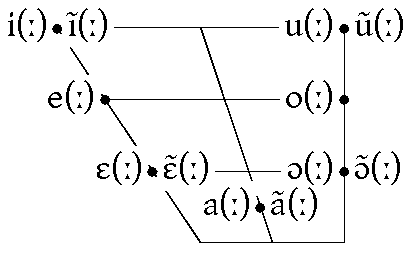
\includegraphics[width=0.4\linewidth]{figures/vowel}
	\caption{Vowel qualities}
	\label{fig:vowel}
\end{figure}

		%There are five phonemic oral and five nasal vowels, and lengthened counterparts:
	
	\begin{table}
		\caption{Minimal pairs for vowels}
		\fittable{\begin{tabular}{llll}
		\lsptoprule
			{[tʰi]} \qu{shell} & {[tʰiː]} \qu{pierce}& {[tɕuvi]} \qu{say standing} & {[tɕuːvi]} \qu{string up}  \\
			& {[wĩː]} \qu{strength} &&\\
			\midrule
			{[tʰe]} \qu{algae}&	{[tʰeː]} \qu{heavy}& {[so]} \qu{roof pole} & [soː] \qu{shoot (bot.)}\\
			{[tʰɛ̃]} \qu{limestone}&{[tʰɛ̃ːn]} \qu{run, fly} &{[tʰɔ̃a]} \qu{command}\footnote{Compare to /tʰo-a/ \qu{call-3\gl{sg}.\gl{obj}}}  &\\
			\midrule
			{[tʰa]} \qu{\gl{ass}}&{[tʰaː]} \qu{tie}&& \\
			{[tʰã]} \qu{feces}&&&\\
		\lspbottomrule
		\end{tabular}}
	\label{tab:phon}
	\end{table}

	
Apart from \textit{wîî} \qu{strength} vs alienable \textit{wii} \qu{field}, [ĩ] is not attested in minimal pairs, I thus treat it as a marginal vowel phoneme. The status of [ũ] is even trickier. 
%\subsection{The phonemic status of [ũ]}	
The nasal closed vowel [ũ] only appears in complementary distribution to its oral counterparts: after the aspirated consonants \textit{kh}, \textit{phw} etc discussed in \sectref{ssec:Aspiration}, after nasals, and in other nasalizing conditions. There are no long nasal vowels in open syllables at all (except [kʰĩː], which is still [kʰĩːk] in closely related Hmwaveke).
	Whether we analyze %/ĩ/ and 
	/ũ/ as a phoneme depends on our understanding of [kʰ]: 
	If [kʰ] is a phoneme, then %[ĩ/ and 
	[ũ] could be analyzed as an allophone of %/i/ and 
	/u/, conditioned by [kʰ]. %Arguments in favour of a phonemic status of [kʰ] are weak: firstly, other languages in the area have /k/ and [kʰ], and secondly, all other non-prenasalized plosives in Vamale have an aspirated phonemic counterpart. There are a few words, such as \textit{kholok} \qu{fall spontaneously} that can be elicited without a nasal vowel, but they are usually recent loanwords. If, on the other hand, we analyzede [kʰ] as a phonologically conditioned allophone  of [k] before nasal vowels, then %[kʰĩː/ \qu{swamp hen} and	[kʰũkʰũ] \qu{mute} is /kũkũ/, and /ũ/ is a marginal phoneme. Last possibility: /ũ/ is maintained in historically nasalized post-\textit{*kn} contexts, but without contrastive pairs, cannot be posited as a phoneme, regardless of the status of [kʰ], which is similarly unclear. 
This description will assume that the distribution of [ũ] is predictable, but will still transcribe [ũ] as \ort{û} except after nasals.
	
	\subsection{Quantity}
	\label{sec:VQuantity}
	\is{Vowels!Quantity}
	Vamale features phonemic length in both monosyllabic words, see the examples \textit{thi} \qu{shell} and \textit{thii} \qu{pierce} at the beginning of \sectref{sec:V} above, and polysyllabic ones.   %Campbell analyzes long vowels in monosyllabic words as underlying sequences of identical vowels in polysyllabic words: /tʰe.ep/ $\rightarrow$ [tʰɛːp] \qu{flow} \parencite[61]{campbell_phenomenon_1987}. This grammar does not. xxwhy not?
	
Consider the following minimal pairs:

\begin{itemize}
 \item\relax [ˈsa.m̥ʷã] \qu{go the other way} vs [ˈsaːm̥ʷã] \qu{banana}
 \item\relax [ˈfa.ti] \qu{language} vs [ˈfaː.ti] \qu{glue something}\footnote{The latter is morphologically complex: \textit{faat} \qu{be sticky} and \textit{-i} \qu{\gl{tr}}}
 \item\relax [ˈtʰa.ke] \qu{throw} vs [ˈtʰaː.ke] \qu{drag}
\end{itemize}
 
This analysis is contested for Voh-Koné languages: Campbell analyzes long vowels in Hmwaveke polysyllabic words as a feature of the stressed syllable \parencite[56]{campbell_phenomenon_1987}. In cases where a fortis-onset syllable takes the stress despite other factors, like the presence of a long syllable (e.g. [ˈtʰa.keː.ke] \qu{stretch out}), or a penultimate syllable (e.g. ['xaⁿ.ɟa.ke] \qu{eat starchy food}), this is argued to be due to extra articulatory energy, but not phonologically stress \parencite[59]{campbell_phenomenon_1987}.

In Vamale, however, many polysyllabic words are composed of only short syllables: e.g. \textit{'ta.na} \qu{ripe}, \textit{'xa.le.ke} \qu{see}, \textit{cu.va.'than.ke} \qu{stand apart}, \textit{'xa.ba.le} \qu{their mat}. Apart from lexical factors, length is conditioned by morphosyntactic factors as well. Possession
	%marked by the suffix \textit{-n} for open syllables, 
	will lengthen the final vowel of some directly possessed, alienable words:
	
	\begin{itemize}
		\item {[ˈfa.ti]} \qu{language} $\rightarrow$ {[fa.ˈtiːn]} \qu{language-3\gl{sg}.\gl{poss}}
		\item {[ˈiː.la]} \qu{cauldron} $\rightarrow$ {[iː.loːŋ]} \qu{my cauldron}
		\item \textit{ˈfʷaːn.dan} \qu{road} $\rightarrow$ {[ˌfʷan.da.ˈnũːŋ]} \qu{my road}
		%\item[/ \textit{}
	\end{itemize}
	
While quantity is phonemic, it is not always realized in everyday speech. Compare \textit{ju} \qu{fish kabob} to \textit{juu} \qu{real, sacred; very}. While the first word is only rarely produced nowadays,\footnote{The loanword \textit{brochette} being used to make the analytical \textit{brochette ko-n nyu} \qu{kabob with fish}} the latter is ubiquitous, and often in an unstressed position, or even a compound (see \sectref{sec:WCIntensifiers}). Both environments tend to elide stress, and unstressed long syllables are often shortened.	
	
\subsection{Quality}
\label{ssec:Vowel_Quality}
\is{Vowels!Quality}
The mid-open vowels have allophones depending on the syllable structure. Open syllables feature closed vowels. Closed syllables have several variables: closed short syllables feature the more open vowels [ɛ] and [ɔ]. Closed long syllables show both pairs; plosive-final syllables have more open vowels ([sɔːt] \qu{touch}), and nasal-final ones feature comparatively more closed vowels ([so̝ːm] \qu{swim}). See \Cref{tab:allovowels} for an illustration. Note that the vowels were rendered here without their nasalization: all vowels preceding nasals are to some degree nasalized, this does not affect with which allophone they are realized.
	
	\begin{table}
		\centering
		
		\caption{Vowel allophones in their defining contexts (nasalization omitted)}
		\begin{tabular}{lll}
			\lsptoprule
			&	[o]	[ɔ] &	[ɛ]	[e]\\
			\midrule
			V	&	[ˈpuːn.dɟo] \qu{whale}		&	[se] \qu{one}\\
			\midrule		
			Vː	&	[ˈtɕoː.lam] \qu{your part /to eat, to do]}		&	[seː] \qu{cry}\\
			\midrule		
			VC	&	[tɕɔp̚] \qu{pass over a ridge}&	[sɛp̚] \qu{coconut}	\\
			&	[ko.ˈkɔt̚] \qu{common mynah (bird)}&	[xɛt̚ ] \qu{warm}	\\
			%	[tʰilowɛc̚/ \qu{kind of tree}	
			&	[pʰɔm] \qu{butterfly}&	[fe.ˈtʰɛm] \qu{white spots (skin)}	\\
			&	[xɔŋ] \qu{my leg}&	[bɛŋ] \qu{waterfall}	\\
			&	[kɔn] \qu{\gl{prog}}&	[sɛn] \qu{poison}	\\
			\midrule		
			VːN	&	[mboːm] \qu{shade}		&	[ɣeːm] \qu{basket}\\
			&	[ɲa.ˈkoːn] \qu{for}		&	[xeːn] \qu{noise}\\
			&	[koːŋ] \qu{on me}		&	[mbeːŋ] \qu{my peer}\\
			\midrule				
			VːP	&	[ɣa.ˈkɔːp̚] \qu{wild}&	[tɛːp̚] \qu{flow (liquid)}	\\		
			&	[tɔːt̚] \qu{grass}, [ɔːt̚] \qu{rope; vein}&	[ˈtɛːt̚] \qu{be lazy}	\\
			\lspbottomrule
		\end{tabular}
		\label{tab:allovowels}
	\end{table}
	
	%Nêlêmwa has V: o and VC ɔ, with some exceptions in long (open and closed) contexts.
	
%	The mid-open vowels before nasals are more open than the ones before orals (compare /tʰe/ \qu{algae} and /tʰɛ̃/ \qu{rock}), meaning that the oral-nasal pairs are not all identical in their aperture.
	Possibly because the community is multilingual, there is considerable variation between individuals concerning the expression of nasality. Some nasalize almost all vowels that follow a nasal, which is why Rivierre does not consider nasality of vowels for Bwatoo, except after oral consonants \citeyearpar[25]{rivierre_bwatoo_2006}. %This conditioned nasalization is also found after the aspirated velar plosive [kʰ], see \Cref{ssec:Aspiration}.
	
	\subsection{Vowel sequences}
	\is{Vowels!Diphthongs}
	\begin{sloppypar}
	There are no diphthongs; recorded vowel sequences are either disyllabic or contain a glide, see \Cref{tab:v_sequences}. Some variants in fast speech seem to reduce the prominence of a syllable and make it approach an on- or offglide quality: /jo.a.kan/ [ˈⁿdɟoa̯.kãn] \qu{thick}.
	\end{sloppypar}
	

\begin{table}
\label{tab:v_sequences}
\begin{tabular}{lll}
\lsptoprule
	~ & Item & Translation  \\\midrule
	ie & [tʰi.en] & \qu{three} \\ 
	io & [ⁿɟi.ɔŋ] & \qu{my belly}  \\
		iu & [pi.uk] & \qu{star} \\ \addlinespace
	ia & [ci.a] & \qu{he is not there}  \\\addlinespace 
	ui & [bu̯i.ɲ̊o] & \qu{type of shell}  \\ 
	ue & [va.tu.e] & \qu{pick pandanus leaves}   \\ 
%uo & [tʰuːp] & shower & also uu, only one?!  \\ \addlinespace
	ua & [tʰu.a] & \qu{clear bush}   \\ \addlinespace
	ei & [pej.pa] & \qu{paper}  \\ 
	eu & [xe.u] & \qu{burn by neglect}  \\ 
	eo & [ⁿde.ɔŋ] & \qu{my spear}\\ 
	ea & [m̥ʷe.ap] & \qu{nest} \\ \addlinespace
	oi & [ᵐbʷa xo.lɔj] & \qu{wheel} \\ 
	oa & [ⁿɟo.a.kan] & \qu{thick}  \\ \addlinespace
	ai & [tʰaj] & \qu{roll up} \\ 
	ae & [mã.ẽ] & \qu{fire} \\ 
	ao & [ha.o] & \qu{grandfather}   \\ 
	au & [sa.ũn] & \qu{garment}  \\ \addlinespace
	uo & * & ~ \\ 
	oe & * & ~ \\ 
	ou & * & ~  \\ 
	\lspbottomrule
\end{tabular}
\caption{Vowel sequences with examples}
\end{table}
	%saun \qu{robe}
	
	\subsection{Allophones of vowels}
	\is{Vowels!Allophones}
Vowel allophony is underdescribed as of yet in Northern languages. Rivierre's detailed phonological description of Cèmuhî \citeyearpar[32, 35, 40]{rivierre_langue_1980} expands upon Haudricourt's brief account of the seven phonemic vowels \citeyearpar[373]{haudricourt_langue_1968}, and considers [ɔ] an allophone of /o/, amongst others. The phonology of the Hienghène languages was studied by \textcite{ozanne-rivierre_phonologie_1982}, but vowel allophones were not mentioned. Yuanga was described in detail by \textcite{schooling_phonology_1992}. There are no phonological descriptions focusing on vowel allophony for Nyelâyû \parencite{ozanne-rivierre_nyelayu_1998} and Nêlêmwa \parencite{bril_nelemwa_2002}.
 	
	\subsubsection{Nasalization of vowels}
	\label{ssec:NasalV}
	\is{Vowels!Nasalized vowels}
	Nasal spreading in both directions is described in detail for Hmwaveke \parencite[66, 76]{campbell_phenomenon_1987}. Vamale has this, too, and both regressive (e.g. [nĩũ] \qu{fish}, (\ref{ex:Vass})) as well as progressive assimilation (e.g. [ãmbu] \qu{\gl{1}\gl{du}.\gl{excl}}, see ex. \ref{ex:Vass2}) to nasals are so frequent that nasality of vowels is most often not phonemic.
	

\ea\label{ex:Vass} 		
[fetãmɛ̃]\\
\gll fe-ta-me\\
		 take-move.up-\gl{dir.cp}\\
\glt \qu{bring up} 
\z


\ea\label{ex:Vass2}
[fɛ̃ãmɛ̃]\\
\gll fe-hân-me\\		
 take-move.same.level-\gl{dir.cp}\\		
\glt \qu{bring (across the same plain)}
\z



	
	%Vowels are often nasalized after nasal consonants, as in Bwatoo \parencite[25]{rivierre_bwatoo_2006}. 
	Nasality also spreads from one vowel to another (regressive assimilation), but does not seem to do so across oral consonants, see (\ref{ex:Vass}). Spreading of nasality is so prevalent in Hmwaveke that Campbell considers it a word-level feature, and that words with truly phonemic nasal vowels are only those that have, among other factors: \begin{enumerate}
		\item no nasal or semi-nasal consonants
		\item and a nasal vowel in the stressed syllable \parencite[66]{campbell_phenomenon_1987}
	\end{enumerate}
	Like nasal vowels, nasalized ones are usually realized more open than their oral counterparts, i.e. /e/ and /o/ are realized as [ɛ̃] and [ɔ̃], respectively. %While nasal /ã/ the vowel in \textit{han} \qu{to walk, to go} is, due to the final nasal, often pronounced [hæ̃n]. 

	
	\subsubsection{Fronting of /u/}
	\label{ssec:fronting_u}
	/u/ is frequently, but not always, fronted to [y] or [ʏ] after the front %(\textbf{	Do you mean immediately after, or in a syllable following a syllable with /i/?})
	 vowel /i/ and its non-syllabic variant [j] (\ref{ex:nyayung}, \ref{ex:xayu}). When asked to pronounce the word as slowly as possible, some speakers like Jaaun Kalène produced [ˈɣaː.e.ʉ] or something further front, while others, like Elise Oué, would have two syllables [ˈɣa.ju]. The latter form is likely to be underlying, as the Pije cognate \textit{ka.hyuk} \parencite[135]{haudricourt_dictionnaire_1982} %and Cèmuhî /áíú/ \parencite[148]{rivierre_langue_1980} suggest a lenition of initial /k/, dropping of final /k/, and a glide between the vowels /a/ and /u/. 
	 suggests that two syllables, with a glide as the second onset, are etymological. While this fronting is not described by Ozanne-Rivierre for Pije, she mentions it for Jawe, as having developed after an intervocalic /v/ was dropped: /ʏi/ \qu{blow} (cf. \textit{uvi} in Fwâi and eastern Nemi) \citeyearpar[22]{ozanne-rivierre_phonologie_1982}. %In Vamale, {[}uŋ] is the allomorph of -\textit{ong} \qu{1\gl{sg}.\gl{poss}} after /i/. This is lexicalized in inalienable lexemes whose stem ends on -\textit{i} (/si-ong/ [sũŋ]\goodtilde[sʏ̃ŋ] \qu{my hand}, /jati-ong/ [ɟatuŋ] \qu{my younger sibling}), but occurs sporadically with other words. A similar phenomenon is described for Nyelâyu \parencite[25]{ozanne-rivierre_nyelayu_1998}, where a realization of /we/ as [ø] in is also discussed.%xhüüli in Kito 
	
	
	\ea\label{ex:nyayung}
%	\ili{}{}{ \textit{nyayung}}
	[ɲãʏ̃ŋ] \goodtilde [ɲãjuŋ]\\
	\gll nyai-ong\\	
	 child-1\gl{sg}.\gl{poss}\\
		\glt \qu{my child}
	\z
	
	
	\ea\label{ex:xayu}
	[ɣaːʏ] \goodtilde [ɣaːju̹]\\
	\gll xayu \\ %\footnotemark\\
	male \\
	\glt \qu{boy, male}
	\z
	
%	\footnotetext{Pije cognate \textit{kahyuk} \qu{man}}
	
	\subsubsection{Backing and rounding of /a/}
	
	/a/ is often backed and centralized in progressive assimilation to labiovelar approximants, a phenomenon also described for Yuanga \parencite[129]{schooling_phonology_1992}. This happens most frequently with \textit{vwa} \qu{do; exist}, especially where it is part of a compound, e.g. \ort{vwa wîîn} [wɒ wĩːn]  \goodtilde [wo wĩːn] \qu{\gl{exist} strength} \qu{be strong}. This is not found in careful pronunciation, but is a regular allophone in Hmwaveke \parencite[16]{campbell_phenomenon_1987}.%, suggesting the phenomenon is at least a century old.
	
%	\subsubsection{Fronting and raising of /a/}
%	
%	
	
	\subsubsection{Interplay between /a/ and \textit{e=} \qu{1\textsc{sg}}}
	
	Some morphemes ending with /a/ will assimilate to the 1\gl{sg} subject index \textit{e=} (\ref{ex:the}). As examples (\ref{ex:cama}) and (\ref{ex:ceme}) show, this process can spread over at least one more syllable, though this depends on the speaker.
	
	\ea
	\label{ex:the}
	(\textit{the bwa han})\\
	\gll tha=e=bwa hân\\
	 \gl{ass}=1\gl{sg}=\gl{ipfv} go\\
	\glt \qu{I am leaving}
	\z
	
	\ea\label{ex:cama}
	(\textit{nyiman cama go vwa})\\
	\gll nyima-n (ca)ma go=vwa\\
	 want-3\gl{sg} \gl{subr} 2\gl{sg}=do\\
	\glt \qu{He wants you to do it.}
	\z
	
	\ea\label{ex:ceme}
	(\textit{nyiman ceme vwa})\\
	\gll nyima-n cam=e=vwa\\
	 want-3\gl{sg} \gl{subr}=1\gl{sg}=do\\
	\glt \qu{He wants me to do it.}
	\z
	
%	\a
%	
%	\ili{}{}{} \textit{tha go hân}
%	\gll tha go hân
%	 \gl{ass}=2\gl{sg} go
%	\glt \qu{You go}
%	
	

	
%	\a
%	
%	\ili{}{}{} cipe caihnan li=aman a go vi
%	\gll cipa e=caihna-n li=aman a go=vi	
%	 \gl{neg} 1\gl{sg}=know-\qu{tr} \gl{def}.\gl{pl}=thing \gl{rel} 2\glsg}=say
%	\glt \qu{I don't know the things you said}
%	
%	
%	
%	\a
%	
%	\ili{}{}{} cipa go caihna-n li=aman \textbf{e} vi
%	\gll 	cipa go caihna-n li=aman a e=vi	
%		\gl{neg} 2\glsg} know-\qu{tr} \gl{def}.\gl{pl}=thing \gl{rel} 1\gl{sg}=say
%	\glt	\qu{You don't know the things I said}	
%	
	
	%Bril thinks this is si-ong with o getting raized, because it overrides the previous vowel in xha-ong . no known reason why only a should suffer. e- because distinctive and the language avoids diphthongs. 
	
	Vamale is the only Voh-Koné language described with this assimilation of /a/ to the first person subject index \textit{e=}. The sequence [ae] appears elsewhere in the language without assimilating (e.g. [ɣa.ˈm̥ã.ɛ̃n] \qu{tomorrow}); the assimilation is specific to the subject marker. It is also noteworthy that this subject marker only occurs in Vamale within Voh-Koné. While neither Hmwaveke nor Pije \parencite[246, 247]{haudricourt_dictionnaire_1982} have subject marker proclitics that differ from the free form, Cèmuhî has a pair /(wa)eo/ vs. /e/ \parencite[61]{rivierre_langue_1980}; Vamale may have borrowed \textit{e=} \qu{1\gl{sg}} from it. The assimilation, however, is not described for Cèmuhî either.
	
	\section{Phonotactics/syllable structure}
	\is{Syllable structure}
	%Contrary to other described Voh-Koné languages, Vamale allows exactly one cluster:
	%\textit{xhwatla} \qu{thunder}. Its cognates are \textit{xhwalaa} in Bwatoo and \textit{xhwala} in Tiéta. A form /xʷalala/ is present in Hmwaveke and could be a preceding form. POc *kuru
	\begin{sloppypar}
	Like its Hienghène and Voh-Koné relatives, Vamale exhibits a (C(ʰʷ))V(VVC) syllable pattern. Pre-nasalized consonants preceded by a vowel (e.g. V\# \#ⁿC, or V.ⁿC) are reanalyzed, and their nasal is assigned to the preceding syllable: /abu/ /am.bu/ \qu{1\gl{du}.\gl{excl}}. %Offglides could be 
	Consonants usually meet at morpheme boundaries, like [wan.ke] \qu{change}, /bofwa-n-mwa/ [bo.fʷan.mʷã] \qu{door, door-of-house}. The only exception found is the morphologically simple word /xʷat.la/ \qu{thunder}, still /xʷa.la.la/ in western varieties.\footnote{In this case, the second syllable /la/ was likely reduced and the cluster fortized to /l̥/, before being split into a stop and a glide.ˈ Most morphologically simple words have one or two syllables.}
	\end{sloppypar}
	
	\section{Reduplication}
	Reduplication is a common morphological process in many Oceanic languages, but plays a negligible role in Vamale. Historically, most old CVCV reduplications, probably already stripped of their morphological function, developed first into CCV geminates through elision of the first syllable's vowel, and then into aspirated plosives or voiceless fricatives (see \sectref{ssec:Aspiration}). Since productive derivational processes work with prefixes%(see \sectref{sec:NomDeriv})
	, the following forms are probably not representative of productive processes.
	\is{Reduplication}
	\is{Negation}
	%Kakai, more polite form of kai \qu{who}
	
	\begin{itemize}
		\item \textit{kokoi}, polite negation, loan from Pije (where \textit{koi} is the negation)
		\item \textit{hahat} \qu{nono}, from \textit{hat} \qu{strong negation}
		\item \textit{sisipo}, \qu{together}, \textit{nya-sipo-ke} \qu{put-together-\gl{tr}}
		\item \textit{fwafwa} \qu{full of holes}, from \textit{fwa} \qu{hole}
		\item \textit{juuju(u)} \qu{truth}, from the root \textit{juu} \qu{true}
		\item \textit{vayavaya} \qu{shaky}, from \textit{vaya} \qu{move}
	\end{itemize}
	
	%xaxahnang \qu{beautiful}, possibly? xa- is a nominalizer but xahnang is maybe not a nominalisable verb? xa- is also a habitual.
	
	\section{Stress}
	\label{sec:Stress}
	\label{sec:stress}
	\is{Stress}
	In Vamale, disyllabic words have penultimate stress, as is typical in Oceanic settings. Trisyllabic, morphologically simple, non-derived nouns take stress on the first syllable, see \Cref{tab:tri}. These are rare, though loanwords now increase their number.

\begin{table}
\caption{Stress in trisyllabic words}
\label{tab:tri}
\begin{tabular}{ll}
\lsptoprule
	Old words & Loanwords\\\midrule
{[}ˈa.pu.li] \qu{person} & {[}ˈᵐbu.ɾu.(w)ɛt] \qu{wheelbarrow},\\
                         & \quad from French [bʁu.ˈɛt]\\
{[}ˈva.ma.le]\qu{vamale}&{[}ˈmãŋ.ga.sĩ] \textasciitilde {[}maŋ.ga.ˈsî/ \qu{shop},\\
                         & \quad  from French {[}magaˈzĩ]\\
{[}ˈⁿdon.dam.ba] \qu{flood garbage}&{[}ˈpu.a.ka] \qu{pig},\\
                         & \quad  from Polynesian \textit{puaka}\\
{[ˈma.vu.lɛn]} \qu{flying fox sp.}&  {[ˈku.mʷa.la]} \qu{sweet potato},\\
                         & \quad  from Polynesian  \textit{kumala}\\
{[ˈma.tʰi.la]} \qu{small bird sp.}&{[}ˈᵑge.ɾe.nũ] \qu{frog},\\
                         & \quad from French \textit{grenouille}\\
\lspbottomrule
%	\item {[ˈⁿdom.bin.do]}  \qu{mangrove eel}
%\item {[ˈpʷa.la.lu]} \qu{rainbow}

%	\item {[}ˈla.lu.ɛn/ \qu{aloe plant}, from French /laloˈɛs]
\end{tabular}
\end{table}

Longer words are morphologically complex and have stress on the penultimate stress-bearing unit, which is often a syllable of the root, but not always. While some morphological factors complicate the picture, regular phonological aspects predict most stress positions. A closed syllable will be stressed over an open one, a fortis onset will usually top a tenuis onset, and a long syllable will be stressed above all else. This gives us a hierarchy of factors:

\ea Long syllable > fortis onset > closed syllable > penultimate syllable
\z
	
%	\begin{table}
%		\label{tab:stress}
%		\caption{Examples for stress in various contexts}
%		\begin{tabular}{lllll}
%			&	\multicolumn{2}{c}{Mono-morphemic}		&\multicolumn{2}{c}{Poly-morphemic}		\\
%			\midrule
%			\multirow{3}{2cm}{open syllable (short)}	&	{[ˈpa.la]} &\qu{speak}		& /ˈpa.la.ke]& \qu{speak /a language]}		\\
%			&	{[ˈfa.to]} &\qu{drink warm}		& /ˈfɛ̃.ã.nã.ke/ &\qu{show}	\\
%			%&	{[ˈfa.va]} &\qu{four}&  &\\
%			\midrule		
%			\multirow{3}{2cm}{open (syllable (long))}	&	{[ˈsaː.m̥ãt]} &\qu{fog}	&	[fu.ˈnãː.ke/ &\qu{preach}			\\
%			& {[ɣe.ˈtʰoː]} &\qu{landing net} & /ˈɣa.fu.nã]& \qu{middle finger (lit. \qu{preacher})}\\
%			& {[ˈmãː.vu]} & \qu{close eyes} &&\\
%			\midrule
%			\multirow{3}{2cm}{closed syllables (short)}&	{[ˈɣaⁿ.ɟe]} &\qu{eat.juicy}  	& /ˈɣa.le.lu/ &\qu{see them}		 \\		
%			&	{[ˈm̥aw.tɕɛp]}& \qu{noni tree}& &		\\	
%			&	{[ˈuⁿ.du]} &\qu{drink cold}&&\\
%			
%			\midrule		
%			\multirow{3}{2cm}{closed syllables (long)}&{[ɣa.ˈkɔːp]}& \qu{wild}&[ɲãˈkõ:ŋ/ &\qu{for me}	\\
%			&{[te.mĩ.ˈnɛ̃ːn]} & \qu{float}& /si.nũ.ˈxiːt]& \qu{painful suffering}\\
%			&{[xa.ˈsaːt]} & \qu{jump}& /fa.ˈto̟ːm]&\qu{your drink}\\
%			\midrule
%			\multirow{4}{2cm}{3 syllables}& 	{[fʷaⁿ.ˈɟi.mʷã]}&\qu{ask}	&	[fʷaⁿ.ˈɟi.mʷã.ke]&\qu{ask (\gl{tr})}	\\
%			&	{[ˈpu.a.ka]} &\qu{pig}	&	[pu.a.ˈka.nɛ̃ɔ̃ŋ/ &\qu{my pig} \\
%			&	{[ˈtʰɔ.a.tit]}& \qu{sky}	&	{[ˈtʰɔ.a.tit̚.tɕa]}	& \qu{this day}\\
%			&   {[pu.ˈpʷaː.le]}& \qu{European} &	[pa.ˈpan.go/ &\qu{your father} \\
%			&	{[tʰe.ˈxʷaːⁿ.de]}& \qu{Tiouandé village}	&[ˈɣaᵐ.bu.na]& \qu{thief}				\\
%			&  {[ˈpʷa.la.lu]} & \qu{rainbow} & & \\
%		\end{tabular}
%		
%	\end{table}
%	

% 	\label{ssec:compF}
\is{Stress!Extrametrical morphemes}
\is{Stress!Complicating factors}
	Some monosyllabic morphemes do not count in the stress pattern. One frequent example is the extrametrical suffix \textit{-ke} \qu{\gl{tr}}, whose phonological non\hyp importance makes the third syllable in /fʷan.ˈɟi.mʷa.ke/ \qu{ask something} the penultimate of the phonological word. %\textit{-ke} may be related to the proclitic \textit{ka} which marks subjects and possessors. 
	Possessive and object-indexing suffixes shift the stress, but not in a simple syllable-counting way, as [ˈᵐbwãn.ɟɛp], [ᵐbwãn.ˈɟɛp.go] \qu{hand drum, hand drum-2\gl{sg}.\gl{poss}} would suggest, i.e. with the stress, all other things being equal, moving to the new penultimate syllable. However, since \textit{bwajep-gavwe} [ˌᵐbwãn.ˈɟɛp.ga.vʷe] \qu{hand drum-2\gl{pl}.\gl{poss}} does not have the stress on the penultimate syllable of the phonological word, [ga], this suggests an analysis of root syllables that is different from that of suffixed morphology. Possessive and object-indexing suffixes count as a single unit in stress assignment, meaning that a two-syllable possessive suffix such as \textit{-gavwe} \qu{2\gl{pl}.\gl{poss}} has the same effect as \textit{-go} \qu{2\gl{sg}.\gl{poss}}.
	
	Speech act participant indexes (the proclitics, not the suffixes) are also extrametrical: 
	
	\begin{itemize}
		\item  /ˈɣa.le.ke/ \qu{to see}
		\item /le=ˈɣa.le-le/ \qu{3\gl{pl}=see-3\gl{pl}.\gl{obj}}, \qu{they see them}
		\item  /le=ɣa.le-ˈkaː.vʷe/ \qu{they see you}, also pronounced /le=ɣa.ˈle.ka.vʷe/ 
	\end{itemize}
%In verbs with long stem vowels, the 
%	%[fʷaⁿ.ˈɟi.mʷa]
%	%fa.ˈlɔŋ.ga.vi
%	[ˈxʷiː.ko]
%	[ˈxʷiː.le]
%	[ˈxʷiː.kavʷe]
\begin{sloppypar}
Other syllables attract stress. The nominalizer \textit{xa-} \qu{\gl{agt}.\gl{nmlz}} (from \textit{xayu} \qu{male}) always attracts stress (probably due to its etymology, see \sectref{ssec:agt.nmlz}), but not the nominalizers \textit{hun-} \qu{manner.\gl{nmlz}} nor \textit{ape-} \qu{place.\gl{nmlz}} (from \textit{ape-n} \qu{trace}).
\end{sloppypar}
	
\begin{table}
		\begin{tabular}{ll}
		{[ˈhun.vʷa ]} \qu{way of doing}&{[a.ˈpe.ta]} \qu{ladder (place of going.up)}\\
		{[hun.ˈmõː]} \qu{way of living}&{[a.pe.ˈmõː]} \qu{dwelling}\\
	\end{tabular}
\end{table}

Semantically bleached function words like /a.ˈman/ \qu{thing; object place-holder} are re-analyzed as one foot in compounds: 
	
	%[ˈxʷi.ja.mãn/ \qu{eat}
\begin{itemize}
	\item {[}ˈtɕaj.n̥ãn] \qu{know}, [tɕaj.ˈn̥ãn.ã.mãn] \qu{know something}
	\item {[}ˈtɕãm.bi] \qu{smash}, [e.tɕãm.ˈbi.jã.mãn]  \qu{hammer}
\end{itemize}
	
The complex word \textit{ape-caihnan-aman-le}, \qu{\gl{nmlz}-know-thing-3\gl{pl}.\gl{poss}} \qu{their knowledge}, is pronounced {[ˌa.pe.tɕaj.n̥ãn.ã.ˈmãn.le]} by Kaina Fouan, which could be explained by analyzing \textit{(ape-)caihnan-aman} \qu{(fact.of-)know-thing} as a compound, \textit{-le} \qu{3\gl{pl}.\gl{poss}} as a suffix, and thus the main stress would fall on the penultimate syllable.
	%The stress seems to be on the root in a complex word, on long vowels, and to be penultimate
	
	%\todo{Find out which words have long vowels}
	%stress in Yuanga is penultimate d.h. calculated from ]#, 
	%intonation is trochäus, 
	%one syllable can contain 2 morae, syllable weight attracts stress
	%accent of trisyyl is on first syll if strong onset energy "attaque", dh aspirated plosives and h
	%composites have different stress but not the verbal tha-, co- things
	
%	\subsubsection{Related languages, their analysis, and how it relates to mine}
For Hmwaveke, stress is described as being fundamentally penultimate \parencite[59]{campbell_phenomenon_1987}, and forms which deviate from this, with few exceptions, are analyzed by Campbell as several phonological words. Campbell analyzes long syllables in plurisyllabic words as resulting from stress (suggesting that, fundamentally, length is a feature of all stressed syllables). For Vamale, though long syllables are stressed, I argue that the relation is reversedː length attracts stress.
 
In Nêlêmwa, stress is usually on the first syllable of the lexical root \textit{kâ-ˈyuva} \qu{how is it? (lit. lying.down-be.thus)} \parencite[26]{bril_nelemwa_2002}. This correlation between morphological structure and stress pattern is mirrored in Vamale to a certain extent, in that bound morphemes such as \textit{e-} \qu{\gl{recp}}, \textit{-ke} \qu{\gl{tr}}, and manner prefixes like \textit{mi-} \qu{do lying down} do not affect the position of the main stress. %The reduplicated form \textit{sisipo} \qu{do together} from \textit{sipo}, still found in \textit{nya-sipo-ke} \qu{put-together-\gl{tr}} is stressed on the first syllable instead of the second, 

	

%	\begin{table}
%		\label{tab:stress}
%		\caption{Examples for stress in various contexts}
%		\begin{tabular}{lllll}
%			&	\multicolumn{2}{c}{Mono-morphemic}		&\multicolumn{2}{c}{Poly-morphemic}		\\
%			\midrule
%			\multirow{3}{2cm}{open syllable (short)}	&	{[ˈpa.la]} &\qu{speak}		& /ˌlu.e.ˈpa.la]& \qu{they speak to each other}		\\
%			&	{[ˈfa.to]} &\qu{drink warm}		& /ˈfɛ̃.ã.nã.ke/ &\qu{show}	\\
%			&	{[ˈfa.va]} &\qu{four}&  &\\
%			\midrule		
%			\multirow{3}{2cm}{open (syllable (long))}	&	{[ˈsaː.m̥ãt]} &\qu{fog}	&	[fu.ˈnãː.ke/ &\qu{preach}			\\
%			& {[ɣe.ˈtʰoː]} &\qu{landing net} & /ˈɣa.fu.nã]& \qu{middle finger (lit. \qu{preacher})}\\
%			& {[ˈmãː.vu]} & \qu{close eyes} &&\\
%			\midrule
%			\multirow{3}{2cm}{closed syllables (short)}&	{[ˈɣaⁿ.ɟe]} &\qu{eat.juicy}  	& /ˈɣa.le.lu/ &\qu{see them}		 \\		
%			&	{[ˈm̥aw.tɕɛp]}& \qu{noni tree}& &		\\	
%			&	{[ˈuⁿ.du]} &\qu{drink cold}&&\\
%			
%			\midrule		
%			\multirow{3}{2cm}{closed syllables (long)}&{[ɣa.ˈkɔːp]}& \qu{wild}&[ɲãˈkõ:ŋ/ &\qu{for me}	\\
%			&{[te.mĩ.ˈnɛ̃ːn]} & \qu{float}& /si.nũ.ˈxiːt]& \qu{painful suffering}\\
%			&{[xa.ˈsaːt]} & \qu{jump}& /fa.ˈto̟ːm]&\qu{your drink}\\
%			\midrule
%			\multirow{4}{2cm}{3 syllables}& 	{[fʷaⁿ.ˈɟi.mʷã]}&\qu{ask}	&	[fʷaⁿ.ˈɟi.mʷã.ke]&\qu{ask (\gl{tr})}	\\
%			&	{[ˈpu.a.ka]} &\qu{pig}	&	[pu.a.ˈka.nɛ̃ɔ̃ŋ/ &\qu{my pig} \\
%			&	{[ˈtʰɔ.a.tit]}& \qu{sky}	&	{[ˈtʰɔ.a.tit̚.tɕa]}	& \qu{this day}\\
%			&   {[pu.ˈpʷaː.le]}& \qu{European} &	[pa.ˈpan.go/ &\qu{your father} \\
%			&	{[tʰe.ˈxʷaːⁿ.de]}& \qu{Tiouandé village}	&[ˈɣaᵐ.bu.na]& \qu{thief}				\\
%			&  {[pʷa.la.lu]} & \qu{rainbow} & & \\
%		\end{tabular}
%		
%	\end{table}
	
	%['xa.wa.xan/ dog or /xa.wa.'xan]?
	%[doː.'hã:/ curry ?
	

\chapter{Word classes} % Main chapter title
\label{ChapterWoCla} % Change X to a consecutive number; for referencing this chapter elsewhere, use \ref{ChapterX}

Vamale words can be divided into several groups according to their syntactic behavior: some big, open classes, some small, closed classes%(e.g. the assertive marker \textit{tha} is unique in its distribution), and a number of forms that exist in several classes %(e.g. \textit{balan} \qu{piece; \gl{cont} marker, just})
, and some with just one member. This chapter will present all of them based on distributional clues. Their names are partly derived from names given to cognate forms in other languages, and in all cases strive to reflect their syntactic function. Verbs, nouns, as well as aspectual markers (here called TAM for ``Tense, Aspect, Mood", presented in \sectref{sec:TAM}), have dedicated chapters later on. Vamale word classes present some aspects of typological interest. Location relative to nouns (e.g. ``on", ``next to") is expressed by derived nominal forms (see \sectref{ssec:WCPrepoNouns}, and not adpositions. There are no adjectives; rather, nominalized verb phrases, or stative verbs. This is discussed in \sectref{sec:adj}. Numerals are not an own word class either: they are formally verbs (see \sectref{ssec:Numerals}). Furthermore, as is common in Oceanic languages, verbs and nouns can be derived from each other with little to no morphology and their morphology overlaps in some cases (see \sectref{ssec:PossV} on verbs with nominal morphology). 
%Notes after FZ 14.02.2019:


\section{What is a word?}
\is{Wordhood}

Words in Vamale exist on several levels (phonological and grammatical), and in a way similar to the zero derivation which affects the verb-noun distinction, words can be reinterpreted and forged anew. As has already been sketched in \sectref{sec:Stress}, \textit{g-words}, i.e. words that act as grammatical units, and \textit{p-words}, i.e. units on a prosodic level with one main accent, do not coincide necessarily. One instance of such mismatches are g-words that attach to other g-words to form a phonological unit \parencite[1]{spencer_clitics_2012}, i.e clitics. Many function words are clitics, e.g. articles. Semantically general g-words which are always part of a phrase, but never its head, and which can be stressed (meaning they are also p-words), will be called ``particles" in this grammar. TAM markers are included in this broad category. The same grammatical element may be a p-word in some construction but part of a larger p-word in others, e.g. \textit{aman} \qu{thing}, and the influence of a word on the stress pattern of its environment can depend on pragmatic factors, such as focus, drawing out a pause to think of something further to add, etc. Furthermore, the boundary between often-used phrases and compounds, is also a fuzzy one (cf. \sectref{ssec:vwa} for an example). Other examples of fluidity between word status and phrase-status are verb phrases or even complete relative clauses which can function as head of a NP by the use of an article (see \sectref{sec:NmlzVP} and \sectref{sec:RelCl} respectively), stative verbs whose nominal morphology makes them useful for adjective-like functions (see \sectref{ssec:Verbs_n}), and serial verb constructions. 

\subsection{Concerning \textit{vwa}}
\label{ssec:vwa}
\is{Wordhood!\textit{vwa}}

The verb \textit{vwa} \qu{do} can combine with a number of morphemes to express an action or a state. It can combine with nouns (e.g. \textit{vwa mwa} \qu{build a house}) and verbs (\textit{vwa tau} \qu{to fish (lit. do hit (the water))}) to form compounds.
The compounds that these combinations create are mostly intransitive verbs with often idiosyncratic meanings: \textit{vwa vua} lit. \qu{do net}, \qu{throw a net}. \textit{Vwa uvu} \qu{do yam}, \qu{wind yam sprouts around a tutor}, \textit{vwa xhwaeo} \qu{do taro}, \qu{harvest taro}. Undergoers would be added as oblique arguments with \textit{ko} \qu{\gl{obl}}, see example (\ref{ex:vwa_ko}). Since \textit{vwa} is semantically vague and thus readily used as a filler verb, new compounds are often formed (e.g. \textit{vwa toki} \qu{do metal}, \qu{make a telephone call}), established compounds can broken up ad hoc into verb phrases with specific arguments (see example \ref{ex:vwa_ref}) and many remain transparent phrases. With few exceptions, this grammar will thus avoid marking \textit{vwa}-constructions clearly as compounds by connecting \textit{vwa} to its modifier or argument. \sectref{sec:ZeroTrans} takes a closer look at intransitive verbs.

\ea \label{ex:vwa_ko}
\gll go\textsubscript{\gl{agt}}=vwa-vua ko {\ob}i=vuman nyu{\cb}\textsubscript{\gl{obl}} nya-xahut\\
 2\gl{sg}=do-net \gl{obl} \gl{def}.\gl{sg}=group fish send-down.there\\
\glt \qu{You cast-net upon the fish school down there.}
\z

\ea \label{ex:vwa_ref}
\gll go\textsubscript{\gl{agt}}=vwa li=xhwaeo\textsubscript{\gl{p}} nya-an\\
 2\gl{sg}=do \gl{def}.\gl{pl}=taro towards-same.level\\
\glt \qu{You harvest the taros over there.}
\z

\subsection{Prosodic words and grammatical words}

Vamale's wealth in different classes of morphemes is mirrored on the phonological level: phonological units overlap or not with syntactic units, and the latter can be derived and re-analyzed relatively easily, compare (\ref{ex:rea1}) to (\ref{ex:rea2}). %For example, nouns that are alienably possessed are marked with -\textit{n} \qu{\gl{poss}}. When the possessor is indexed via a personal possessive suffix (1\gl{sg} etc.) rather than a noun, the possessed noun takes the suffixes \textit{-n-eong, -n-go, -n-gau},\ldots See \Cref{tab:morph_overview} for a complete list. 
Possessive constructions follow a head-first pattern: \gl{psm}-\gl{poss} \gl{psr}. The personal possessive suffixes mirror the construction found with nouns, and are cognate with ``indirect" possessive constructions in other languages, where the possessor is expressed as a pronoun, e.g. Pije \textit{thala-n nyan} \qu{knife-\gl{poss} 3\gl{sg}} \parencite[248]{haudricourt_dictionnaire_1982}. However, there are some arguments in favor of a suffix analysis: 
\begin{enumerate}
	\sloppy
	\item The 1\gl{sg} form \textit{-eong} and the 3\gl{sg} form \textit{-ea} are not identical (anymore) with the free pronouns \textit{io} and \textit{ia}.
	\item The syllabification now includes the formerly external possessor markers (i.e. \textit{puakan-ea} [pu.a.ˈka.nɛ̃.ã] \qu{pig.\gl{poss}-3\gl{sg}.\gl{poss}})
	\item The stress shift towards the last syllable before the possessive suffix: [ˈtʰa.la] \qu{knife} $\rightarrow$ [tʰa.ˈla.nɛ̃.ã] \qu{knife-3\gl{sg}.\gl{poss}}
\end{enumerate}


\ea\label{ex:rea1}
[ˌhɲ̊ĩmãke eˈtɕaːmãn]\\
\gll hnyimake (eca)=aman\\
 think.about \gl{indf}.\gl{sg}=thing\\
\glt \qu{think about something.}
\z


\ea\label{ex:rea2}
[i.ˌhɲ̊ĩ.mãˈke.a.mãn]\\
\gll i=hnyimake-aman\\
 \gl{def}.\gl{sg}=think-thing\\
\glt \qu{the thinking of something}
\z	
	
%They are pronounced like suffixes. Given the absence of infixes, I must try to squeeze something inbetween.

\subsection{Affixes and clitics}
\is{Wordhood!Affixes}
\is{Wordhood!Clitics}
\begin{sloppypar}
Vamale morphemes cover much of the spectrum of grammatical wordhood: forms that are units on both syntactic and phonological grounds, some that are either one or the other, and some flexibility depending on the context.  
This grammar will follow \textcite{spencer_clitics_2012} in defining clitics: A clitic is a form of a word which is phonologically attached to another word, its host. Clitics cannot be stressed, there cannot be a pause between them and their host, they have the same functions as g-words, and can attach to various kinds of syntactic units \parencite[1]{spencer_clitics_2012}.
\end{sloppypar}

\begin{enumerate}
	\item Verbs, nouns, and adverbs are g-words as well as p-words, because they can move relatively freely and can be stressed.
	\item Subject markers and articles are proclitics, tied to a predicate (verbal or nominal), and noun phrase respectively, they cannot be stressed.
	\item Aspectual markers are particles because they are phonologically autonomous, but since they are grammatically dependent on predicates, Zúñiga's term ``anti-clitic" may be more precise \parencite{zuniga_anti_2014}.

\end{enumerate}

%\begin{itemize}
%	\item	i=xhong
%	\item	i=juu xhong
%	\item	i=joakan sapwen
%	\item	i=juu joakan ma juu xhopwen juu sapwen-eong (the real thick and real big traditional garment of mine)
%	
%	
%	\item	e=xaleke
%	\item	e=juu xaleke
%	\item	e=bwa juu xaleke
%	
%	\item	e=xale-a
%	\item	*e=xale juu a
%	
%	\item	sinu-ong
%	\item	*sinu 
%\end{itemize}

\section{The distinction between verbs and nouns}
\is{Wordhood!Verbs vs nouns}
A common problem in Oceanic linguistics concerns the distinction between verbs and nouns, which can be considered blurry. A verb phrase can be nominalized just by putting an article in front of it, after which it functions as an argument. A noun phrase can be used as a predicate, and preceded by aspect and modality markers. As discussed by \textcite[3]{creissels_non-verbal_}, one can distinguish three types of non-verbal predicates: nominal, adjectival, and locative. Vamale has no adjectives, but nominal and locative predicates are well attested. example (\ref{ex:le_niehni}) is an example of a pronominal predicate, (\ref{ex:ca_i_bureau}) shows a predicative locative noun phrase, composed of a prepositional noun \textit{ca} \qu{in} and a common noun, and a nominal predicate is shown in (\ref{ex:predN}). 


\ea\label{ex:le_niehni}
%% \ili{}{}{} 
\gll li=bee-m, le=niehni\\
 \gl{def}.\gl{pl}=peer-2\gl{sg}.\gl{poss} 3\gl{pl}=all.those\\
\glt \qu{Your friends, they are those over there.} {[}X4:14]
\z



\ea\label{ex:ca_i_bureau}
%\ili{}{}{} KG:515
\gll cahma patron ya tha=a=juu ena a ca i=bureau hihihi\\
 \gl{top} boss 3\gl{sg} \gl{ass}=3\gl{sg}=very \gl{dist} 3\gl{sg} in \gl{def}.\gl{sg}=office \\
\glt \qu{The boss however, there he was in his office.} {[}KG:515]
\z


%here? e=daahma. "i am (a) chxxief." grammar works on the basis of predicates, not verbs. subject markers attach to predicates, not "verbs". 

%Example of \textit{la} for null-derivation:
%\ea
%\a
%
%\ili{}{}{} 2019-07-22 JP see me: 14
%\gll lu=moo ca la a=see la
%
% 3\gl{du}=stay in be.here \gl{rel}=same be.here
%
%\glt \qu{They stay in the same place (lit they stay in a place that is there )}
%
%
%\z

\ea\label{ex:predN}
\gll go=bo i=daahma\\
 2\gl{sg}=\gl{irr} \gl{def}.\gl{sg}=chief\\
\glt \qu{You would be chief.}
\z


The transitive suffix \textit{-ke} can be found in or at the end of nouns, but only nouns of verbal origin. 
\begin{itemize}
%	\item \textit{xhwi aman} \qu{eat something, food}
	\item \textit{hnyimake} \qu{think, pay attention}, \textit{hnyimake-aman} \qu{think something}, \textit{i ape-hnyimake-aman} \qu{\gl{def}.\gl{sg} \gl{nmlz}-think-thing}, \qu{the thought}
	\item \textit{vwa-siteke} \qu{Sunday, (lit. do-sacred, pray)}
	\item \textit{e-topweeke-aman} \qu{hook, (lit. \gl{nmlz}-hang-thing)}
%	\item \textit{ba} \qu{wall}, \textit{bake} \qu{stack stones}
%	\item fubun \qu{heap}, \textit{fubuuke} \qu{make a heap of something}
\end{itemize}

\subsection{Syntactic criteria}

While nouns and verbs share some syntactic slots, and some nouns and verbs may look the same (see \sectref{ssec:PossV}), and many of the words surrounding both noun and verb phrases have shared origins, like \textit{ma} \qu{\gl{subr}, \gl{com}}, \textit{ko} \qu{on, \gl{obl}}, or \textit{xhwat} \qu{a small piece}, \qu{a little bit}, there are differences still: nouns cannot take arguments, they have different modifiers, and if TAM markers are used, they do not mean the same thing.
Numerals, for instance, are verbs because they take arguments, e.g. \textit{se-a} \qu{the only one, he is one/alone}, \textit{thaloo mu mani} \qu{the birds are two}, \textit{thien li=ba} \qu{the sardines (are) three}. \textit{Nievit} \qu{how many} works the same way: \textit{Nievit sinan xat?} \qu{how.many sign sun}, \qu{what time is it?}.%, singular maybe because the answer can be \textit{se} "one", or because the referent of \textit{sinan} is a sign on the clock? \textit{Nievit-le}.

Within a noun phrase, modifiers are either nominalized verbs that precede the noun, as in (\ref{ex:WCadj1}), possessors, or relative clauses, as in (\ref{ex:WCadj2}). Verbal modifiers are either adverbs or adverbial clauses, or verbs that integrate the verb phrase. 


\ea\label{ex:WCadj1}
\gll i=bwaakala a=xhopwen\\
 \gl{def}.\gl{sg}=boat \gl{rel}=big\\
\glt \qu{the big boat}
\z


\ea\label{ex:WCadj2}
\gll i=joakan sapwen\\
 \gl{def}.\gl{sg}=thick dress\\
\glt \qu{the thick dress}
\z 

%Distributional not clear, but morphological and semantic criteria. Hier erwähnen: Adjektive werden wie ersetzt? Sind die anders als andere Verben?

\subsection{Morphological criteria}
\label{ssec:morph_crit}
\is{Morphology}
\begin{sloppypar}
Verbs and nouns share some morphology, most notably possessive suffixes. While these suffixes are examined in more detail in \sectref{ssec:PossV} and \sectref{ssec:active-n} for verbs, and in \sectref{sec:Poss} for nouns, an overview is provided in \Cref{tab:morph_overview}. Inalienable (I and Ib) and alienable (II) possessive suffixes can thus occur on verbs, either to mark the undergoer-like subject of some stative verbs or the undergoer argument of some active transitive verbs. 
\end{sloppypar}
 
\begin{table}
	\centering
	\caption{Possessive suffixes, \textsc{obj} and -\gl{S\textsubscript{P}}}
	
	\begin{tabular}{llccccc}
	\lsptoprule
	%	&&&\multirow{3}{}{Possession}&&&\\
		&& I& Ib& II & -\gl{S\textsubscript{P}} &\gl{obj}\\\midrule
\gl{sg} &	1&	\textit{-ng}&	\textit{-ong}&	\textit{-eong} &\textit{-ong} & \textit{-eo}\\
		&	2&	\textit{-m}&	\textit{-am}&	\textit{-go}&\textit{-go} & \textit{-ko}\\
		&	3&	\textit{-n}&	\textit{-an}&	\textit{-ea} & \textit{-(e)a} & \textit{-}a \\
		\midrule
\gl{du} &	1\gl{incl}&\textit{-ju}&	\textit{-aju}&\textit{-ju} &\textit{-gaeu/-gasu} &\textit{-kaeu}\\
		&	1\gl{excl}&	\textit{-bu}&	\textit{-abu}&	\textit{-bu}& \textit{-gabu}&\textit{-kabu}\\
		&	2&	\textit{-u}&	\textit{-au}&	\textit{-gau} &\textit{-gau} & \textit{-kau}\\
		&	3&	\textit{-lu}&	\textit{-alu}&	\textit{-lu }&\textit{-lu} & \textit{-lu} \\
		\midrule
\gl{pl} &	1\gl{incl}&	\textit{-j}e&\textit{-aje}&	\textit{-je} &\textit{-gaa} & \textit{-kaa}\\
		&	1\gl{excl}&	\textit{-be}&	\textit{-abe}&	\textit{-be} & \textit{-abe}&\textit{-kabe} \\
		&	2&	\textit{-vwe}&	\textit{-avwe}&	\textit{-vwe} &  \textit{-gavwe}& \textit{-kavwe}\\
		&	3&\textit{-le}&\textit{-ale}&	\textit{-le} & \textit{-le }&\textit{-le}\\
	\lspbottomrule
	\end{tabular}
\label{tab:morph_overview}
\end{table}
 
Reflexive/reciprocal \textit{e-}, mostly found on verbs, also occurs with nouns in predicate function, as shown in (\ref{ex:refl_nouns}–\ref{ex:refl_nouns2}). This is a relatively rare occurrence and was only attested with a reciprocal meaning.

\ea \label{ex:refl_nouns}
%\ili{}{}{} vamale-180809-1:00:15:20
\gll lu=e-\textit{copain}-\textit{copine}\\
 3\gl{du}=\gl{recp}-boyfriend-girlfriend\\
\glt \qu{The two are boyfriend and girlfriend.} {[}vamale-180809-1:00:15:20]
\z


\ea \label{ex:refl_nouns2}
\gll calibeen ma le=moo ma li=ehni, e-bee-le\\
 sometimes \gl{subr} 3\gl{pl}=stay \gl{com} \gl{def}.\gl{pl}=\gl{dem}.\gl{prox}  \gl{recp}-peer-3\gl{pl}.\gl{poss}\\
\glt \qu{Sometimes when they stay together with those, they are each other's cousins.} {[}AG1:239]
\z

Some particles and affixes, however, mark the resulting construction as definitely verbal. This includes causative \textit{fa-}, transitive markers \textit{-ke} and \textit{-i}, and manner prefixes (discussed in \sectref{sec:Manner}). For example, \textit{xhaavwa} in (\ref{ex:xhavwa}) has a different stem than \textit{xhavwaleke} in (\ref{ex:xhavwaleke}), both in vowel quantity and the last syllable \textit{-le}.


\ea\label{ex:xhavwa}
\gll e=xhaavwa\\
 1\gl{sg}=wait\\
\glt \qu{I'm waiting around.}
\z

\ea\label{ex:xhavwaleke}
\gll e=xhavwale-ke (aman)\\
 1\gl{sg}=wait.for-\gl{tr} something\\ 
\glt \qu{I'm waiting for something.}
%\a
%
%\gll xa-xhavwale-ke (aman)
% \gl{nmlz}-wait.for-\gl{appl} something 
%\glt \qu{Someone who waits for something}
%
\z

Object markers in general are sure signs of verbhood. §\ref{sec:WC_nouns}--\ref{sec:WC_sbjka} below will explore the noun phrase with its members: articles, nouns, demonstrative and personal pronouns (followed by the subject marker proclitics which are historically related), and some case markers.

TAM markers, which, like subject markers, are shared by both predicative nouns as well as verbs, will form the link in this chapter between the two big groups. Verbs will only be sketched here, as they form the most diverse and biggest word class of the language. After introducing adverbs, smaller classes, often with a wider scope, will be introduced.

%\subsubsection{\textit{-n}}
\is{Specificity!\textit{-n}}
The suffix \textit{-n} \qu{\gl{nspec}, \gl{ana}} warrants an early introduction, as it occurs across word classes, affecting dependent verbs, prepositional nouns and regular inalienable nouns alike. In essence, \textit{-n} has two functions: one is to mark the generic nature of the argument of its verbal host (\ref{ex:verbal-n}), or the generic possessor of its nominal host (\ref{ex:nominal-n}), while the other function is anaphoric or cataphoric. Generic nouns do not take an article, whereas specific nouns take definite or indefinite articles (see \sectref{sec:WCArticles}). 


\ea\label{ex:verbal-n}
\gll ka na naen cipa hmwaka-n habu\\
 \gl{cnj} \gl{dem} now \gl{neg} be.like-\gl{nspec} long.ago\\
\glt \qu{But this is today, not like [things were) yesterday.} {[KP:12]}
\z


\ea\label{ex:nominal-n}
\gll kon th=e ra-ta-meebam nyeca-n sohmun\\
 then \gl{ass}=1\gl{sg} \gl{nmlz}-be.sitting-sleep inside-\gl{nspec} school\\
\glt \qu{You must know that I kept sleeping on my chair at school.} {[PE1:187]}
\z 

%Two other suffixes \textit{-n} must be mentioned: in noun phrases, a suffix \textit{-n} indexes inalienable 3\gl{sg} possessors on the possessed noun, be it specific (\ref{ex:inalienable}) or generic (\ref{ex:nspec}). Another suffix \textit{-n} serves as an alienable possessum-marking construct suffix (no indication of person), as in (\ref{ex:alienable}) (see \sectref{sec:Poss} for a more detailed discussion). The two \textit{-n} are distinguished on the basis of their different distribution. Inalienable \textit{-n} \qu{3\gl{sg}.\gl{poss}} is part of a paradigm of possessive pronoun marking suffixes, excluding a possessor NP following, while the construct suffix has no allomorphs, grammatically conditioned or otherwise, and occurs between a nominal possessor and its possessum. As the (in)alienability of nouns is lexically conditioned, the two suffixes do not contrast on the same word.
%
%
%\ea\label{ex:inalienable}
%\gll i=bwa-n/-m\\
% \gl{def}.\gl{sg}=head-3\gl{sg}.\gl{poss}/2\gl{sg}.\gl{poss}\\
%\glt \qu{his/your head}
%\z
%
%
%\ea\label{ex:nspec}
%\gll i=bwa-n apuli\\
% \gl{def}.\gl{sg}=head-3\gl{sg}.\gl{poss} human\\
%\glt \qu{the human head}
%\z
%
%
%\ea\label{ex:alienable}
%\gll i=mwa-n i=apuli\\
% \gl{def}.\gl{sg}=house-\gl{poss} \gl{def}.\gl{sg}=person\\
%\glt \qu{the house of the person}
%\z

The suffix \textit{-n} \qu{\gl{nspec}, \gl{ana}} is analyzed as one single suffix despite its distribution both on nouns and verbs, as it always marks the head of the phrase and the generic nature of its dependents. \is{Specificity! Generic \textit{-n}}

%\todo{s that a possessive marker ?	You need to give a closer analysis of these –n, not just give them labels, to demonstrate their category and function}

\is{Anaphoric \textit{-n}}The other function mentioned above is anaphora in the wider sense: relating to something already mentioned (\ref{ex:n_ana}), mentioned in another clause soon after, or known in general (\ref{ex:hmwaana_koon}). The referent's specificity is not important in this case. %The syntactic roles avalailable to the participant indexed with \textit{-n} are lower ones: objects, the modifiers of prepositional phrases, and, in the case of nominalizations featuring \textit{ka-n}, intransitive or inanimate subjects. 


\ea\label{ex:n_ana}
\gll ehni xhwan da, abe=fate gavwe koo-\textbf{n} go abe=sate-\textbf{n}, cipa hmai-n, cipa-bu ju-vaa udu hmwaka-u\\
 \gl{prox} little what 1\gl{pl}.\gl{excl}=share 2\gl{pl} \gl{obl}-\gl{ana} then 1\gl{pl}.\gl{excl}=be.different-\gl{ana} \gl{neg} be.many-\gl{nspec} \gl{neg}-1\gl{du}.\gl{excl} real-too drink like-2\gl{du}\\
\glt \qu{This [wine and beer) is nothing much, we share with you of this, and [as for) us, it's different, not much, we don't drink as hard as you do.} {[L2:3]}
\z


\ea\label{ex:hmwaana_koon}
\gll hmwaa-na koo-n!\\
 like-\gl{dist} on-\gl{ana}\\
\glt \qu{Like that!/Now that's a proper way of doing it!}
\z

\subsection{Semantic criteria}

As in other Kanak languages \parencites[89]{bril_nelemwa_2002}[32]{rivierre_bwatoo_2006}, there are few roots exclusively dedicated to one category, and they are mostly nominal roots. Examples include kinship terms, body parts, topographical and meteorological terms, many animals and plants, as well as parts of the house, boats, and tools. 

\section{Articles}
\label{sec:WCArticles}
\is{Articles}
%members: \textit{i}/\textit{vi}, \textit{mu}, \textit{ni}/\textit{li}, \textit{muca}, \textit{eca}, \textit{ca}
%\\criteria: come before a noun, are part of the NP
%\\size: 6

%\input{specific_parts_documents/i_and_ka/i.tex}

Vamale has a fine-tuned system of definiteness, using both definite and indefinite articles for specific reference, and the absence of articles for non-specific (i.e. less transitive) scenarios. This closed word class is called ``articles" in this grammar because its members precede nouns and mark them as (in)definite.
Vamale makes the wide-spread distinction between singular, dual and plural (see \Cref{tab:articles}), and what this study considers to be degrees of definiteness rather than specificity (an argument for this analysis follows in \sectref{ssec:WCArt_specificity}). Using a noun phrase without an article makes it non-specific, as seen in (\ref{ex:noArt2}) and (\ref{ex:Art2}). 

\ea\label{ex:noArt2}
\gll go=han can hnyimake thamo\\
 2\gl{sg}=walk \gl{subr} think woman\\
\glt \qu{You walk while thinking about a woman.} {[G4:22]}
\z


\ea\label{ex:Art2}
%\ili{}{}{} G4:22
\gll go=han can hnyimake i=thamo\\
 2\gl{sg}=walk \gl{subr} think \gl{def}.\gl{sg}=woman\\
\glt \qu{You walk while thinking about the woman.}
%\is{Subordination!Adverbial clause}
%\ea
%
%\gll e=xaleke apuli \textbf{a}=kon xhwi puaka 
% 1\gl{sg}=see man \gl{rel}=\gl{prog} eat pig
%\glt \qu{I see a man who is eating pork/a pig.}
%
%\a
%
%\gll e=xaleke apuli a=kon xhwi i=puaka 
% 1\gl{sg}=see man \gl{rel}=\gl{prog} eat \gl{def}.\gl{sg}=pig
%\glt \qu{I see a man who is eating the pig.}
%
\z

\begin{table}
	\caption{Articles in Vamale}
	\begin{tabular}{lll}
	\lsptoprule
		&\gl{spec} and \gl{def}& \gl{spec} and \gl{indf}\\\midrule
		\gl{sg} & \textit{i} & \textit{(e)ca} \\
		\gl{du} & \textit{mu} & \textit{muca}  \\
		\gl{pl} & \textit{li} / \textit{ni} & \textit{ca(been)} \\
	\lspbottomrule
	\end{tabular}
\label{tab:articles}
\end{table}

The article can combine with the stative verb \textit{se} \qu{one, same} and the noun \textit{been} \qu{peer} to mean \qu{the/some other}. This is further discussed in \sectref{sec:ise}.

%FZ: I am not sure this is the best way to put it -- do you mean "se" can be used predicatively (e.g. 'it is one') as well as attributively (like here, lit. 'the man who is one')? Does your theory of parts of speech work like that, viz. (suitable) verbs can occupy both syntactic(/pragmatic) slots? 
Vamale speakers can choose between using an article (the noun thus having a specific referent) (see \ref{ex:Art}), and not using an article (see \ref{ex:noArt}, \ref{ex:gen}), in which case the noun is generic. In oft-used expressions, the verb forms a compound with the noun.\footnote{See \textcite{ozanne-rivierre_verbal_2004} for a discussion of similar phenomena in other New Caledonian languages.}


\ea\label{ex:Art}
\gll e=xaleke i=apuli a=a=xhwi i=puaka\\
	1\gl{sg}=see \gl{def}.\gl{sg}=man	\gl{rel}=3\gl{sg}=eat	 \gl{def}.\gl{sg}=pig\\
\glt	\qu{I see the man who is biting the pig.}
\z

\ea\label{ex:noArt}
\gll		e=xaleke i=apuli 	a=a=xhwi puaka\\
		1\gl{sg}=see \gl{def}.\gl{sg}=man 	\gl{rel}=3\gl{sg}=eat pig\\
\glt		\qu{I see the man who is eating pork.} (not: the/a/some pig)
		\z

%\begin{comment}
%\a
%
%\gll e=xaleke apuli a=xhwi puaka	
%	}=see man	\gl{rel}=eat  pig
%\glt \qu{I see a man who is eating pork/a pig.}	
%
%\end{comment}

\ea\label{ex:gen}
\gll lu=xa-tena apuli\\
 3\gl{du}=\gl{hab}-understand person\\
\glt \qu{They understand people.}
\z



\subsection{The question of definiteness}
\label{ssec:WCArt_specificity}
\begin{sloppypar}
Vamale articles are split, as can be seen in \Cref{tab:articles}, not only according to their number, but along another axis, definiteness. 
%\subsection{The singular article \textit{i}.}	
 %who speaks Fwâi, Nemi, and understands Pije and Vamale. 
%I suggested a first translation, which was almost completely re-written by the workgroup. The entire text can be found in \Cref{text:beat}. 
Consider example (\ref{ex:t1}) from a French\hyp language legend, written by Yvonne Sahilé, and translated by the workgroup into Vamale. The example translates \qu{il y avait une tribu} (there was a tribe) using \textit{i} \qu{\gl{def}.\gl{sg}}, making it seem more specific than definite, since the listeners cannot yet be familiar with the tribe. My first suggestion was using an indefinite article \textit{eca}  (\ref{ex:wrongtipije}), which was refused. %The whole text is too long to be shown here, but see the document "conte". 
Now look at example (\ref{ex:t1}), where the tribe has never been mentioned before, compared to examples (\ref{ex:t2}) and (\ref{ex:t3}), where it has. All sentences use the same article. In (\ref{ex:t3}), \textit{li thamo} \qu{the women} are newly introduced to the narrative but marked with the definite \textit{li}. %It could be argued that there are always young women in a village, but the previous argument of saliency to the situation seems to justify an analysis as definite well enough.
\end{sloppypar}

\ea
\label{ex:wrongtipije}
%\ili{}{}{}  
\gll *Habu can vije vwa eca=ape-moo a= pwan jelan ehni i=jahoot-ca a= xhopwen.		\\
 long.ago in Tipije \gl{exist} \gl{indf}.\gl{sg}=\gl{loc}.\gl{nmlz}-stay \gl{rel}= on side \gl{dem}.\gl{prox}  \gl{def}.\gl{sg}=river-\gl{prox} \gl{rel}= big	\\
\glt  {[1, authors's attempt]}		
\z

\ea\label{ex:t1}
\gll 	Habu Can-Vije vwa \textbf{i}=apemoo a= pwa-n jela \textbf{i}=jahoot a= xhopwen.	\\
	long.ago Tipije \textit{exist} \gl{def}.\gl{sg}=tribe \gl{rel}= on-\gl{nspec} side \gl{def}.\gl{sg}=river \gl{rel}= big	\\
\glt  \qu{Long ago in the Tipije valley, there was a tribe on the bank of this great river.} (following the French original text)	{[1]}	
\z

\ea\label{ex:t2}
\gll 	Ca i=apemoo-ca le=vacuti \textbf{ca} daahma a= bwa xawe, ka yata-n Thêa Xa-vila	\\
	in \gl{def}.\gl{sg}=tribe-\gl{prox} 3\gl{pl}=erect some chief \gl{rel}= \gl{ipfv} young and name-3\gl{sg}.\gl{poss} T. \gl{nmlz}-dance	\\
\glt  \qu{In this tribe they erected a chief who was still young, and his name was Firstborn the Dancer.} (Thêa is a name commonly given to the firstborn son)	{[2]}	
\z

\ea\label{ex:t3}
\gll Ca \textbf{i}=apemoo vwa \textbf{li}=xawe thamo	\\
 in \gl{def}.\gl{sg}=tribe \gl{exist} \gl{def}.\gl{pl}=young woman	\\
\glt \qu{In the tribe were young women.} (indefinite, non-specific in the French original) {[3]}	
\z

This description analyzes \textit{i} \qu{\gl{def}.\gl{sg}} and \textit{li} \qu{\gl{def}.\gl{pl}} as definite articles, using \textcite{lyons_definiteness_1999}'s definition. Noun phrases marked with \textit{i} and \textit{li} are identifiable \parencite[1]{lyons_definiteness_1999}, albeit not necessarily familiar \parencite[3]{lyons_definiteness_1999}, see (\ref{ex:t2}) and (\ref{ex:t3}). Familiarity, to Lyons, is not an necessary feature for a construction to be definite \parencite[5]{lyons_definiteness_1999}. As Lyons discusses in the pages following that statement, the uniqueness of a referent, in total or relative to the context \parencite[8]{lyons_definiteness_1999}, or even ``the totality of the objects [\ldots] in the context which satisfy the description'' \parencite[11]{lyons_definiteness_1999}, can all be grounds for definiteness. 

Example (\ref{ex:t4-6}) describes a woman not previously mentioned, \textit{\textbf{eca} thamo a en maa-n} \qu{she who has a beautiful face}: indefinite but specific. Example (\ref{ex:t7}) describes a similar situation: In-Thu is a unique, identifiable character, not previously introduced. However, the relative clause modifying her is defining, and so preceded by \textit{i}, whereas the one in (\ref{ex:t4-6}) is not, and its modified noun takes \textit{eca}. %The use of definite \textit{i} instead of indefinite \textit{eca} may be a de-grammaticalized one, however: \textit{eca} is not attested before defining relative clauses, but can occur before an indefinite. 
Example (\ref{ex:t2}) seems to use \textit{ca} in an indefinite way, too, introducing a character who is then further specified and named. %But is it specific? They could have elected some chief, whoever he was, and only afterwards is it explained how he is called.
%\todo{zu spannend}

\ea\label{ex:t4-6}
\gll tha fe nyamaa-n ca-n dawee-le \textbf{eca} thamo a= en maa-n. ka a=xhani ma mwada-n.
Yata-n In Fwe\\
 \gl{ass}.3\gl{sg} take eye-3\gl{sg}.\gl{poss} in-\gl{nspec} between-3\gl{pl}.\gl{poss} \textbf{some} woman \gl{rel}= first face-3\gl{sg}.\gl{poss} and 3\gl{sg}=choose \gl{subr} wife-3\gl{sg}.\gl{poss} name-3\gl{sg}.\gl{poss} skin guettarda.speciosa \\
\glt \qu{Some woman among them \qu{caught his eye}, who was the most beautiful. And he chose her as his wife. Her name was Figtree Bark.}	{[GC:4-6]}
\z

\ea\label{ex:t7}%
(Note the \textit{i a yatan} construction, \qu{the who name-her})\\
\gll le=kiica ka meeka \textbf{li}=been thamo, ma ca-n e-dawee-le \textbf{i}=a= yata-n In Thu.	\\
 3\gl{pl}=jealous and all \gl{def}.\gl{pl}=other woman \gl{com} in-\gl{indf} \gl{mid}-between-3\gl{pl} \gl{def}.\gl{sg}=\gl{rel}= name-3\gl{sg}.\gl{poss} skin banyan\\
\glt \qu{All the other women were jealous, with among them all the one who was called Banyan Bark.} {[}GC:7]	
\z

%More examples from the same text:

%\ea
%\a
%
%\gll 	Kavi tha go xaleke i\textsubscript{def}=[e kon xaleke], na hmuun mae
%	but \gl{ass}=2\gl{sg} see \gl{def}.\gl{sg}=\gl{rel}.1\gl{sg} \gl{koon} see \gl{dem} smoke fire	
%\glt  \qu{But do you see what I'm seeing, that's firesmoke}		
%
%
%\a
%
%\gll 	Hmwakan vwa apuli\textsubscript{NSPEC} xada, gasu bo fwajimwa nyaanya
%	maybe \gl{exist} person up.there 1\gl{du}.\gl{incl} \gl{fut} ask mum	
%\glt  \qu{Maybe there are people up there, we'll ask Mum}	
%
%
%\a
%
%\gll 	Cala lu fwajimwe-a, a vwa e-vwaseekan ka In Fwe ko a caihna-n hapi na la i\textsubscript{def} xhoogo-nea		
%	when 3\gl{du} ask-3\gl{sg} 3\gl{sg} do \gl{ins}-sad \gl{sbj} I. F. because 3\gl{sg} know.\gl{inan} \gl{comp} \gl{dem} be.here \gl{def}.\gl{sg}=home-3\gl{sg}.\gl{poss}	
%\glt  \qu{When they asked her, Fig Bark was sad because she knew that this was her home.}		
%
%
%\a
%
%\gll 	Ka a sabe nya.sii-lu \qu{hmwakan vwa apuli\textsubscript{NSPEC} xada}	
%	and 3\gl{sg} lift.to.mouth give.hand-3\gl{du} maybe \gl{exist} people up.there	
%\glt  \qu{And she answered them ``maybe there are people up there"}		
%
%
%\a
%
%\ili{}{}{} Ungrammatical: *\textit{ca hmuu-n mae-aen}
%\gll 	Ca i wadan a e-thaloo-kan tha see ma i a vi, kavi a vi nyakolu hapi ca \textbf{eca} se wadan gase bo ta xaleke i hmuu-n mae-aen.		
%	in.\gl{def} \gl{def}.\gl{sg}=time \gl{rel} \gl{ord}-two-\gl{ord} \gl{ass}.3\gl{sg} cry \gl{com} \gl{def}.\gl{sg}=\gl{rel}.3\gl{sg} say, \gl{cnj} 3\gl{sg} say to-3\gl{du} that in some other time 1\gl{pl}.\gl{incl} \gl{fut} go.up see	\gl{def}.\gl{sg}=smoke-\gl{poss} fire \gl{dem}
%\glt  \qu{The second time she cried about what he said, but she told them that some other time(singular) we'll go up and/to look at that smoke.}		
%
%\z
%
%\ex
%
%\gll Ko i si-n thu cipa le xaleke \textbf{eca} mani a xhwatiin yata-n mathila ko a kon fwajimwake hapi na kai ni-ehni a le kon bwaa hma.	
% on \gl{def}.\gl{sg}=arm-\gl{poss} banyan \gl{neg} 3\gl{pl} see some bird \gl{rel} small name-3\gl{sg}.\gl{poss} M. but 3\gl{sg} \gl{koon} ask that \gl{dem}  who \gl{def}.\gl{pl}-\gl{prox}\gl{rel} 3\gl{pl} \gl{koon} \gl{ipfv} arrive	
%\glt \qu{They didn't see some small bird on the banyan branch called Mathila [\textit{Rhipidura} \textit{spilodera} \textit{verreauxi} Marie] but it was wondering who these people were who had just arrived.}	
%
%\z

Vamale distinguishes specific from generic participants using articles (except for pronouns and proper names). The articles mark number and definiteness, and, through their presence, specificity. The criteria for definite noun phrases include identifiability and uniqueness, as shown in (\ref{ex:t4-6}), where a woman is introduced as one of many, compared to the obligatorily definite introduction of the unique village in (\ref{ex:t1}).

\subsection{The articles \textit{ca} and \textit{eca} \qu{some}}
\label{ssec:eca}
The article \textit{eca} cannot co-occur with any of the definite articles \textit{i}, \textit{mu}, \textit{li}, nor with a demonstrative pronoun in the same phrase.\footnote{The adverb \textit{eca-ve} \qu{some-where} probably combines the stative verb \textit{ve} \qu{where? (immobile)} with the article, as does \textit{eca-se} \qu{some-one} (\ref{ex:eca}).} \Cref{tab:Pwpw} also suggests that \textit{ca}-forms are used as articles, with \textit{la} cognates in Hienghène-linkage languages.


	\ea \label{ex:eca}
	\gll	eca-aman \\
		some-thing \\
	\glt	\qu{something}% (\textit{aman} is also a placeholder for arguments of certain verbs, like \textit{xhwi aman} \qu{eat something})
	\z
	
	\ea
	%\ili{}{}{} \textit{se} can be inflected like a stative verb (\textit{se-a} \qu{he is alone; the only one})
	\gll	eca-se	\\
		some-one/other\\
	\glt	\qu{someone}
	\z
	
	\ea%
	(Vamale Usa)\\
	\gll eca-ve(n) xada	\\
	 some-where up.there	\\
	\glt \qu{somewhere up there}	
	\z


While \textit{eca} is used in compounds with singular meaning (\ref{ex:eca}), the distinction between singular and plural indefinite articles is becoming blurry. 
\textit{Ca} \qu{\gl{indf}.\gl{pl}} is distinguished by older speakers from \textit{eca} \qu{\gl{indf}.\gl{sg}}, but not anymore by many younger speakers, where the two forms are in relatively free variation. The extent to which this distinction is still important is illustrated in the examples (\ref{ex:ca_eca_old}). According to Jeo Kalène (40 years old),\footnote{Recorded on 12.11.2018, see the archive.} \textit{eca} is the singular and \textit{ca} the plural indefinite article (\ref{ex:ca_eca_old}). 

%Maybe example \ref{ex:ca_oven} is different from example \ref{ex:ca_field}, and more akin to \ref{ex:ca_xhuam}. In  \ref{ex:ca_oven} and \ref{ex:ca_xhuam}, \textit{ca} refers to parts of uncountable \qu{masses} (food in one case, things to put in her oven in the other). It is probably related to \textit{ca(-n)} \qu{in (it)} (see \ref{ex:t2}). In \ref{ex:ca_field}, \textit{ca} refers to a place, but more importantly, \textit{it does not modify a noun}. The clause in brackets is subordinate to \textit{hân fwadai} \qu{go look for it} and \textit{la} \qu{be here} is anaphoric, but does it refer to \textit{ca}, or something implied? \textit{ca} is a preposition for nouns with an article.


\ea \label{ex:ca_eca_old}
\gll tha vwa eca=apuli a= a=vwa hmwaena	\\
 \gl{ass} \gl{exist} some.\gl{sg}=person \gl{rel}= 3\gl{sg}=do thus.\gl{dist} \\
\glt	\qu{There is a person who does it like this.}
\z

\ea
(\textit{ca} and \textit{a} \qu{3\gl{sg}} cannot refer to the same participant)\\
\gll *tha vwa \textbf{ca}=apuli a= \textbf{a}=vwa hmwaena	\\
 \gl{ass} \gl{exist} some.\gl{pl}=man \gl{rel}= 3\gl{sg}=do thus.\gl{dist}	\\
\glt (for:\qu{There is a man who does thus.})	
\z

\ea
(\textit{eca} and \textit{le} cannot refer to the same participant.)\\
\gll *tha vwa \textbf{eca}=apuli a= \textbf{le}=vwa hmwaena	\\
 \gl{ass} \gl{exist} some.\gl{sg}=man \gl{rel}= 3\gl{pl}=do thus.\gl{dist}	\\
\glt (for: \qu{There is a/some man who does thus.})	
\z

\ea
\gll tha vwa ca=apuli a= le=vwa hmwaena	\\
 \gl{ass} \gl{exist} some.\gl{pl}=man \gl{rel}= 3\gl{pl}=do thus.\gl{dist}	\\
\glt	\qu{There are people who do it like this.}
\z


\ea \label{ex:ca_been}
\gll e=xaje ca=been\\
 1\gl{sg}=eat.juicy \gl{indf}.\gl{pl}=peer\\
\glt \qu{I ate some of them.} {[vamale-181127-jp\_nelemwa-1: 00:05:02]}
\z

%2018-12-17: 
\textit{Cabeen}, probably from \textit{ca been} \qu{some others, some of them}, see (\ref{ex:ca_been}), is for 25-year-old Jean-Philippe Oué the unambiguous plural form of \textit{eca}, whereas \textit{ca} is a free variant of \textit{eca}, but can also be used for the plural. A similar confusion is found in the examples below, which stem from the translated legend (the translators were all around 40–50 years old). The article in (\ref{ex:ca_oven}) could refer to plural or singular entities, but in (\ref{ex:ca_field}) would more refer signify a single place.


%\a
%
%\ili{}{}{} (context)
%\gll Fine bwaabwen pathaabua i juu mwa a mu hmaako-n xeen uvu, xeen xhwaeo, nyu ma juu-mani  
% count morning before \gl{def}.\gl{sg}=real house \gl{rel} 3\glu} find-\gl{nspec}	basket yam basket taro fish \gl{com} real-bird
%\glt  \qu{Every morning she found before the hut baskets of yam, taro, [she found] fish and \textit{notou} [huge, sacred forest pigeons \textit{Ducula goliath}]}		
%
\ea \label{ex:ca_oven}
\gll ma cika vuki-n ma a=xaahni \textbf{ca}=aman ma a=vwa tââ-n\\
 \gl{subr} \gl{neg}.\gl{exist} reason-\gl{poss} \gl{subr} 3\gl{sg}=look.for \gl{indf}.\gl{pl}=thing \gl{subr} 3\gl{sg}=make oven-3\gl{sg}.\gl{poss}	\\
\glt \qu{So that there was no reason for her to seek something to make her oven (with) (i.e. cook).}
\z

\ea \label{ex:ca_field}
\gll i=bwaabwen-an a=ja han fwadai \textbf{ca}\textsubscript{i}= {\ob}ma a=vwa nyangan-aman la\textsubscript{i}{\cb}\\
 \gl{def}.\gl{sg}=morning-\gl{poss}	3\gl{sg}=\gl{prf} go search.\gl{inan} some= \gl{subr} 3\gl{sg}=do garden-something be.here\\
\glt \qu{The next day (lit. its morning) she finally went to look for some place to make her field.}	
\z

Since number is not marked on nouns, both (\ref{ex:ca_oven}) above and (\ref{ex:ca_xhuam}) below may actually denote non-singular rather than plural, since both refer to non-singular, possibly uncountable referents.
%\todo{make up your mind viz. foodstuffs}
\ea \label{ex:ca_xhuam}
\gll		fe   ca=xhua-m 	\\		
		take \gl{art}.\gl{indf}.\gl{pl}=food-2\gl{pl}.\gl{poss}\\
\glt		\qu{Take some food (lit. Take some of your foodstuff).}
\z
%\a
%
%\gll		*fe   can  xhua-m 			
%		take in food-2\gl{pl}.\gl{poss}
%%\glt		%\qu{Take some food [lit. Take some of your foodstuff(s?)]}
%
%\z	
\subsection{Variation: \textit{li} vs \textit{ni}}
\label{ssec:ni}
%Whatever do you mean by this "distinctions of the past" ? It's opaque to me!



%The relevant data are shown below in table \ref{tab:pije_articles}.
%\begin{table}
%	\centering
%	\label{tab:pije_articles}
%	\caption{Articles in 1970s Pije.}\
%	\begin{tabular}{l|lll}
%		&	\multicolumn{2}{c}{\gl{def}}	&		\gl{indf} \\
%		&	\gl{spec}& \gl{nspec}&\\ 
%		SG& vin & vi & va\\
%		DU& [maan \textit{in Fwâi}] &maali & maala\\
%		PL& ni & li=& la\\
%	\end{tabular}
%	
%\end{table}

%Usa Vamale does not seem to use two different forms \textit{li} and \textit{ni} either, as the examples below show. 
%
\ea \label{ex:ni}
%% \ili{}{}{} 
\gll	ma 	le=tha-vwa ni ape-mae\\
	\gl{subr} 3\gl{pl}=strongly-do		ni		\gl{loc}.\gl{nmlz}-fire\\
\glt		\qu{And they start fires/make the fire places (not like before, they light too many fires now).} {[0:01:29 of vamale-171129-ecology (Usa)]}
\z
%
%
%\ea
%		
%\gll		vwa-ila-hn ea  go    ni   nyai-le  nya tha   le  moo xahut pedaa
%		do-pot-\gl{poss} 3\gl{sg}.\gl{poss} then n. child-3\gl{pl}.\gl{poss} put \gl{ass}=3\gl{pl} stay down  P.
%\glt \qu{...cook him, then their children ? They stayed down in Pindache.} 
%
%
%\ea
%	
%\gll		le 	tha 	vwa  tha  	vwa 	ni 		apuli a		thii mae
%		3\gl{pl} 	\gl{ass} 	do    \gl{ass} 	exist 	\gl{indf}.\gl{pl}? 	man \gl{rel}	light fire
%\glt		\qu{They do, there are people lighting fires}
%\ili{}{}{} 	>>>What I would have expected: \textit{Tha le vwa, tha vwa ni apuli}. The assertive is always used before the predicate in coastal Vamale, but maybe this is more flexible in Usa. Another possibility would be that \textit{le} is thematic and outside of the clause, and the structure is something like \textit{le\textsubscript{1}, [tha vwa\_\textsubscript{1}], [tha vwa ni apuli]}.
%	
%\z		
%One more form was recorded once:	\textit{kane} \gl{def}.\gl{pl}=in modern Pije (\textit{ni} in 1970s). Used by one person in Vamale once (her parents speak Pije), see example \ref{ex:kane}. This seems at the very least to indicate that the system is not as rigid as it used to be.
%\ex \label{ex:kane}
%		
%\gll		Juu 	vwa-wîî-n 		xat 	xhwii 	ka 	kane 	nyabu
%		very 	be-strong-3\gl{sg} 	sun 	bite 	\gl{sbj} k. 		mosquito
%\glt		\qu{[The] sun is very strong, the mosquitoes are biting" (Facebook message, speaker lives in Pije-dominant tribe but does not speak Pije)}
%
%\z	


\subsection{Other, related languages}	

Articles are a widespread feature of Oceanic languages \parencite[38]{lynch_oceanic_2002}. They are also common in Mainland New Caledonian languages, with the exception of Far Northern Nêlêmwa, which uses different verbal suffixes to dinstinguish specific from non-specific objects, and possibly Nyelâyu, where abbreviated demonstratives can act as articles \parencite[43]{ozanne-rivierre_nyelayu_1998}. All Northern languages use articles, from Jawe \parencite[255]{haudricourt_dictionnaire_1982} to Paicî \parencite[177]{rivierre_dictionnaire_1983}. Interestingly, though language contact and multilingualism were common and encouraged until at least the early 20\textsuperscript{th} century, article systems are not identical. Cèmuhî, for example, distinguishes nouns along personified/neutral and female/non-female axes \parencite[144]{rivierre_langue_1980}. The Hienghène systems distinguish definite, definite specific, and indefinite, where Vamale only has a definite/indefinite distinction (see \Cref{tab:hyehen_articles}). Bwatoo is described to have two plurals (but only one dual): an unmarked one, and a ``restricted" one, which is used for groups of known or cohesive elements \parencite[42]{rivierre_bwatoo_2006}, a feature which was not found in Vamale.

\begin{table}
	\caption{The article system in 1970 Hienghène languages \parencite[255]{haudricourt_dictionnaire_1982}}
	\begin{tabular}{l lll}
	\lsptoprule
			  &\multicolumn{3}{c}{Singular}\\
		      &\textsc{def}          & \textsc{def} \textsc{sp}                    & \textsc{indf}\\\midrule
		Pije  & \textit{vin}\footnote{This may be a complex form, with \textit{-n} \qu{\gl{nspec}}.} 
                             & \textit{vi}                 & \textit{va}               \\ 
		Fwâi  & \textit{ven} & \textit{veli}               & \textit{vera}             \\ 
		Nemi 1& \textit{vin} & \textit{vi}                 & \textit{va}               \\ 
		Nemi 2& \textit{ven} & \textit{vi}/\textit{veli}   &\textit{vera}/\textit{va}  \\ 
		Jawe  & \textit{nei} & \textit{di(i)}              & \textit{ya}               \\\midrule
		
		&\multicolumn{3}{c}{Dual}\\
			   &\textsc{def}          & \textsc{def} \textsc{sp}                    & \textsc{indf}\\\midrule
		Pije   &               &\textit{maali}   & \textit{maala}\\    
		Fwâi   & \textit{maan} & \textit{maali}  & \textit{maara}\\    
		Nemi 1 & \textit{maan} & \textit{maali}  & \textit{maara}\\    
		Nemi 2 & \textit{maan} & \textit{maali}  & \textit{maara}\\    
		Jawe   &               & \textit{deuli}  & \textit{deulixen}\\\midrule
		
		&\multicolumn{3}{c}{Plural}\\
		      &\textsc{def}          & \textsc{def} \textsc{sp}                    & \textsc{indf}\\\midrule
		Pije  & \textit{ni}   & \textit{li}                & \textit{la}\\
		Fwâi  & \textit{ngen} & \textit{ngeli}/\textit{li} & \textit{ngera}\\
		Nemi 1& \textit{ni}   & \textit{li}                & \textit{ra}\\
		Nemi 2& \textit{ngen} & \textit{ngeli}             & \textit{(nge)ra}\\
		Jawe  &               & \textit{deeli}             & \textit{deelixen}/\textit{yaxen}\\
		
		\lspbottomrule
	\end{tabular}
\label{tab:hyehen_articles}
\end{table}

The more archaic Vamale variety Usa kept \textit{v-} in its articles, which is found in Pwaamei, Pije as well, and was dropped in Vamale (see \Cref{tab:Pwpw}). \textit{Muu-hni} \qu{\gl{du}-\gl{prox}, those two} is frequent, and \textit{mu-ca} \qu{\gl{du}-\gl{indf}} accepted, following the Pwaamei logic of \textit{vaabu}\slash\textit{vaabu-ca} (see \Cref{tab:eca}). A combination of dual article and demonstrative suffix (in this case, a proximate visible one) is thus possible, and results in a demonstrative pronoun.

\begin{table}
		\caption{Pwaamei Hnaakâ (1a) / Pwaamei Yaak (1b) / Pwapwâ (2) / Bwatoo (3) / Usa (4) articles in: \parencite[94,95]{ozanne-rivierre_dictionnaire_} (1–2) and \parencite[42]{rivierre_bwatoo_2006} (3), fieldwork 2017 (4).}
	%\cite{ozanne-rivierre_dictionnaire_} 
	%\parencite[]{rivierre_bwatoo_2006}
	\begin{tabular}{l lllll}
	\lsptoprule
				& \multicolumn{5}{c}{\gl{def}}\\ 
				&1a             & 1b             & 2              & 3               & 4\\
				\midrule
		\gl{sg} & \textit{ve}   & \textit{vi}    & \textit{de}    &\textit{a / (a)ni} &\textit{vi(n)}   \\  
		\gl{du} & \textit{vaabu}& \textit{vaabu} & \textit{duuli} &?                &\textit{mu}   \\  
		\gl{pl} & \textit{ni/i} & \textit{ni/i}  &\textit{i/dili} &\textit{(le)ni}  &\textit{ni (li)} \\  
				\midrule
				& \multicolumn{5}{c}{\gl{indf}}\\
				& 1a& 1b & 2 &3 &4\\
				\midrule
		\gl{sg} & \textit{veca}    & \textit{vica}   & \textit{deca}   &?&\textit{veca} \\
		\gl{du} & \textit{vaabuca} & \textit{vaabuca}& \textit{duulica}&?&?  \\
		\gl{pl} & \textit{ca}      & \textit{ca}     & \textit{ca}     &?&?\\
	\lspbottomrule
	\end{tabular}
	\label{tab:Pwpw}
\end{table}


\begin{table}
	\centering

	\caption{Bwatoo articles}
	\begin{tabular}{lll}
	\lsptoprule
		\gl{sg} & \textit{a} & \textit{(a)ni} \\
		\gl{du}& \textit{(a)lu} & \textit{luni}\\
		restricted \gl{pl} & \textit{(a)le} & \textit{leni}\\
		\gl{pl} & \multicolumn{2}{c}{\textit{ni}} \\
	\lspbottomrule
	\end{tabular}
	\label{tab:Bwatoo_art}
\end{table}


\begin{table}
	\caption{Pwaamei\slash Pwapwâ articles in \citet{ozanne-rivierre_dictionnaire_}}
	\begin{tabular}{l lll lll}
	\lsptoprule
			   & \multicolumn{3}{c}{\gl{def}}   & \multicolumn{3}{c}{\gl{indf}}\\\cmidrule(lr){2-4}\cmidrule(lr){5-7}
			   & Pwm Hnaakâ & Yaak & Pwapwâ     & Pwm Hnaakâ & Yaak & Pwapwâ\\\midrule
		\gl{sg}& \textit{ve} & \textit{vi}      & \textit{de} &\textit{veca} & \textit{vica}& \textit{deca} \\
		\gl{du}& \textit{vaabu}& \textit{vaabu} & \textit{duuli} & \textit{vaabuca}&\textit{vaabuca}& \textit{duulica}  \\
		\gl{pl}& \textit{ni/i}& \textit{ni/i}   &\textit{i/dili} & \textit{ca}& \textit{ca}& \textit{ca}\\
	\lspbottomrule
	\end{tabular}
	\label{tab:eca}
\end{table}

%Things that can go between a noun phrase and its article: normally none (with the exception of the items discussed in \sectref{ssec:statVnomM}, and \textit{i-se} \qu{the other}, \textit{ca-been} \qu{the others} etc).

The definite articles \textit{i} and \textit{li} can derive relative clauses to nouns (\ref{ex:art_RC}).
\newpage

%\begin{multicolumns}{2}
		
	\ea \label{ex:art_RC}
		% \ili{}{}{} 
	\gll le=vwa ma le=thabilo li=a= le=fee-ko\\
	 3\gl{pl}=do \gl{subr} 3\gl{pl}=strike \gl{def}.\gl{pl}=\gl{rel}= 3\gl{pl}=take-2\gl{sg}.\gl{obj}\\
	\glt \qu{They want to kill those who took you.} {[B1:8]}
	\z
	
	
	\ea
	\gll na i=a= vwa wîî-n\\
	 \gl{dem} \gl{def}.\gl{sg}=\gl{rel}= \gl{exist} strength-3\gl{sg}.\gl{poss}\\
	\glt \qu{That's the strong one (among them).} {[JV:11]}
\z
%\end{multicolumn}



%Articles are not described in much detail in the literature so far, so to what extent the system presented here is extraordinary or typical will have to be answered in coming years.


\section{Demonstratives}
\is{Pronouns!Demonstrative pronouns}

Demonstrative pronouns have nominal status in the sense that they function syntactically as nouns including case marking, except that they cannot take articles. Vamale demonstratives distinguish proximal and distal (see \Cref{tab:demonstratives}), making the system somewhat simpler than the regional three-way average \parencite[38]{lynch_oceanic_2002}. They are a closed class of six forms, whose members are only partially transparent. All forms contain a distal or proximal suffix, and the dual forms still carry as a stem the dual article \textit{mu}. The plural forms' stem \textit{ni} is identical to the plural article in Usa Vamale and other Voh-Koné varieties \parencite[42]{rivierre_bwatoo_2006} discussed in \sectref{ssec:ni}, and is accepted by most speakers of Vamale as well. The segment \textit{e-} in the singular forms may derive from the singular article \textit{i} and the plural forms could be composed of plural article \textit{ni} and the singular, already lexicalised form. Demonstrative pronouns can serve both as topic and comment, as in (\ref{ex:WCdem}). 

\begin{table}
	\caption{Demonstrative pronouns}
	\begin{tabular}{lll}
	\lsptoprule
		& Proximal & Distal\\
		\midrule
		\gl{sg} & \textit{e-hni} & \textit{e-na}\\
		\gl{du} & \textit{muu-hni} & \textit{muu-na}\\
		\gl{pl} & \textit{ni-e-hni} & \textit{ni-e-na}\\	
	\lspbottomrule
	\end{tabular} 
\label{tab:demonstratives}
\end{table}



\ea \label{ex:WCdem}
\gll cahma \textbf{ehni} a=mu tua tua i=aman\\
 \gl{top} \gl{dem}.\gl{prox} 3\gl{sg}=\gl{freq} unwrap unwrap \gl{def}.\gl{sg}=thing \\
\glt \qu{But him, he was unwrapping, unwrapping the thing.} {[GS:76]}
\z


\ea
\gll li=thôa koon, li=e=paa vii \textbf{ehni} a= kon mo cahni\\
 \gl{def}.\gl{sg}=custom.object \gl{obl}-\gl{nspec} \gl{def}.\gl{pl}=1\gl{sg}=\gl{prf} say \gl{dem}.\gl{prox} \gl{rel}= \gl{prog} stay here\\
\glt \qu{The ceremonial objects I mentioned are these, which are lying here.} {[ET:1]}
\z 


%\subsection{\textit{na} \qu{\textsc{dem}}, \textit{ha} \qu{\textsc{dem.rep}}}

The demonstrative pronoun \textit{na} is special, because it can be used as a presentative (``this is Liline"), and to mark the comment of an equational clause (\ref{ex:na_topic1}, \ref{ex:na_topic2}). Since \textit{hni} does not exist (anymore), \textit{na} is neither proximal nor distal, and functions as a more neutral pronoun.


\ea\label{ex:na_topic1}
\gll {{\ob}}na{\cb}\textsubscript{{\upshape NP}} {\ob}vaang {\ob}hapi {\ob}{\ob}na{\cb}\textsubscript{{\upshape NP}}{\cb} {\ob}Lilin{\cb}\textsubscript{{\upshape NP}} a {\ob}{\ob}na=mwa{\cb}\textsubscript{{\upshape NP}} {\ob}Liiz{\cb}\textsubscript{{\upshape NP}}{\cb}\textsubscript{{\upshape clause}} a{\cb}\textsubscript{{\upshape\gl{subr}.clause}}{\cb}\\
 \gl{dem} unknown \gl{comp} \gl{dem} L. or \gl{dem}=\gl{rep} L. or\\
\glt \qu{It's unclear if it was Liline or if it was Lise or...} {[KG:472.1]}
\z

\ea\label{ex:na_topic2}
\gll Jacob tha juu xa-vee ma hmwaana. \textbf{na} hmwaana, go=xaleke?\\
 J. \gl{ass} real \gl{nmlz}.\gl{agt}-fuck \gl{subr} thus \gl{dem} thus 2\gl{sg}=see\\
\glt \qu{Jacob, it's bad for him if it's like this. That's how it is, you see?} {[KL:122.1]}
\z

\section{Nouns}
\label{sec:WC_nouns}
\is{Nouns}

Vamale nouns are defined in this grammar as syntactic units which can bear articles. Few other properties distinguish nouns from verbs, but nouns can be arguments to verbs, %(and as such often be counted)
most of them can be possessed (though possessive morphology shows overlaps with some verbal morphology, see \sectref{sec:StatV}), and though they do take some TAM marking, not all TAM marking is attested for nouns (examples include \textit{bwa balan} \qu{\gl{ipfv} \gl{cont}}, \textit{ja} \qu{\gl{prf}}). Nouns are an open class and are described in detail in \Cref{ChapterNouns}. Two noun classes are closed, however: classifiers and relational nouns.

\subsection{Classifiers}
\label{ssec:WCClass}
\is{Nouns!Classifiers}
Vamale possesses several types of classifiers, most prominently two types of relational classifiers, one type for food and drink items (\textit{xhua-} \qu{proteiny food}, \textit{ya-} \qu{starchy food}, \textit{udoo-} \qu{cold drink}, etc.), and one more type for parts of plants. Their occurrence is semantically specified. This class is described in more detail in \sectref{sec:CL}.
The descendant of the general possessive classifier POc *na has become a construct suffix \textit{-n} marking alienably possessible nouns. Another morpheme, \textit{ka}, marks alienable, semantically vaguely ``dynamic" relations (see \sectref{ssec:ka_CL}). Similar morphemes are called general classifiers by several authors \parencite{lichtenberk_oceanic_2009,lichtenberk_possessive_1985,lynch_historical_2000}. However, because \textit{ka} is syntactically different from typical classifiers (it is not the head of its phrase, it has no clear semantics and it is optional in many cases), I simply call it a linker here (following e.g. \cite{bril_ownership_2012}): a morpheme part of the head noun's noun phrase, introducing a modifier noun phrase.

\subsection{Relational nouns}
\label{ssec:WCPrepoNouns}
\is{Prepositions!Relational nouns}

Relational nouns are the functional equivalent of spatial prepositions in Vamale, meaning they are the head of a phrase. Their modifier\slash possessor is the location in which the noun phrase or verb phrase's referent is located (\ref{ex:pwa1}). The members of this closed class are possessed (mostly inalienably) and cannot take an article. They are included with nouns because of their historical relationship to nouns % xxaskAlexElias
 and their possessive morphology. The members are listed in \Cref{tab:relationalnouns}. They are inalienably possessed, except for \textit{cai-n} \qu{behind an animate entity}. 
 
\begin{table} 
\caption{Relational nouns}
\begin{tabular}{ll}
\lsptoprule
 	  \textit{xala-n} &\qu{under} \\ 
 	  \textit{cela-n} & \qu{next to} \\ 
 	  \textit{pwa-n} &\qu{on top of} \\ 
 	  \textit{pwan bwa-n}& \qu{on (top of)} \\ 
 	  \textit{cakebwa-n} &\qu{on the other side} \\ 
 	  \textit{(can) dawee-n} &\qu{(in-) between} \\ 
 	  \textit{ca-n} &\qu{in, at} \\ 
 	  \textit{can hawâ-n} &\qu{facing} \\ 
 	  \textit{ko-n}& \qu{on} \\ 
 	  \textit{pathabua-n} &\qu{before (spatial and temporal)}\\
	  \textit{cai-n} & \qu{behind an animate entity}\\   
\lspbottomrule
\end{tabular}
\label{tab:relationalnouns}
\end{table}

Some of the relational nouns are derived from nouns using a devoicing of the first consonant, e.g. \textit{bwa-n} \qu{head, top} $\rightarrow$ \textit{pwa-n} \qu{on top}, \textit{jela-n} \qu{side} $\rightarrow$ \textit{cela-n} \qu{next to}. This phenomenon is also described for Cèmuhî \parencite[37]{rivierre_langue_1980}.  Inalienably possessed relational nouns like \textit{xala-n} \qu{under} all lose their final \textit{-n} if followed by a specific argument (\ref{ex:pwa}). 


\ea\label{ex:pwa1}
%\ili{}{}{}
\gll a=xheela-ta pwa-n ye\\
 3\gl{sg}=crawl-go.up on-\gl{indf} tree\\
\glt \qu{He tree-climbs.}
\z

\ea\label{ex:pwa}
%\ili{}{}{}
\gll  a=xheela-ta pwa i=ye\\
 3\gl{sg}=crawl-go.up on \gl{def}.\gl{sg}=tree\\
\glt \qu{He climbs the tree/a tree.}
\z


\section{Independent personal pronouns}
\label{sec:WCPersPron}
\is{Pronouns!Personal pronouns}
\begin{table}
	\caption{S – free form}
	\begin{tabular}{l llll}
	\lsptoprule
		       & 1 (\gl{excl})&	1+ (\gl{incl})&	2&	3\\\midrule
		\gl{sg}&	\textit{yo}&&		\textit{go}&	\textit{ya}\\
		\gl{du}&	\textit{abu}&	\textit{gasu}&	\textit{gau}&	\textit{lu}\\
		\gl{pl}&	\textit{abe}&	\textit{gase}&	\textit{gavwe}&	\textit{le}\\
	\lspbottomrule
	\end{tabular}
	\label{tab:freePN1}
\end{table}

Vamale uses the eleven pronominal forms listed in \Cref{tab:freePN1}, distinguishing singular, dual, and plural, as well as inclusive and exclusive first persons. 
The forms are independent pronouns in the sense that they can take up the same slot as a nominal phrase. The difference to subject marker clitics is that the pronouns cannot co-occur with another noun phrase that has the same syntactic function. Subject index clitics are always present (except in imperatives, or in stative verbs with inanimate subjects). This means that, at least following the Uniqueness Condition asking for each grammatical relation to be assigned only once within its clause (after \cite[19]{kroeger_analyzing_2004}), subject indexing clitics (or ``bound pronouns") and free personal pronouns are not allomorphs. Compare to \Cref{tab:markers}. Pronouns can take subject markers (see example \ref{ex:PNcase}), but not articles.

\ea \label{ex:PNcase} 
\gll e=vii ka yo\\
 1\gl{sg}=say \gl{sbj} 1\gl{sg}\\
\glt \qu{I say.}
%\a
%
%\gll *i=mwa-n-le li=apuli
%
% \gl{def}.\gl{sg}=house-\gl{poss}-3\gl{sg}.\gl{poss} \gl{def}.\gl{pl}=person
%
%\glt (for: the house of the people)
%
%
\z


\section{Subject-indexing bound pronouns}
\label{sec:WCSubjProCl}
\is{Subject indexes}
As mentioned in \sectref{sec:WCPersPron}, Vamale uses proclitics derived from free pronominal forms, in order to index subject NPs on active verbs (see \Cref{tab:markers}). Note that stative verbs mark the intransitive subject much like alienable possessums do (compare \Cref{tab:PossSuffix1}). The clitics occur before active verbal, or nominal predicates, in the slot left of the TAM markers. The pair \textit{yo} \textasciitilde \textit{e=} \qu{1\gl{sg}} is the same in Cèmuhî \parencite[61]{rivierre_langue_1980}, but not in other Voh-Koné languages. The other markers are transparently Voh-Koné, and almost identical with the western varieties: \ort{zha} [ða] \textasciitilde \ort{a} [a] \qu{3\gl{sg}} is described for Bwatoo as well \parencite[31]{rivierre_bwatoo_2006}. The sound correspondence [ð] \textasciitilde [j] is a regular one between coastal and mountain varieties. Note that while the bound pronouns are mostly very similar to the free pronouns, they can co-occur in the same clause (\ref{ex:subject_index}), which is a sign that they do not have the same syntactic role: the free forms are true pronouns, whereas the bound pronouns have become grammaticalized to subject indexes on predicates.% the free form \textit{ya} \qu{3\gl{sg}} seems to be a loan from the Pije form \textit{nyang} or Fwâi \textit{yak} \qu{3\gl{sg}} \parencite[246]{haudricourt_dictionnaire_1982}. 

\begin{table} 
	\centering
	\caption{Subject and object markers for active and stative verbs}
	\begin{tabular}{lllll}
		\lsptoprule
		&	Free form	& \gl{a}=/\gl{S\textsubscript{A}}= & -\gl{S\textsubscript{P}} & -\gl{p}\\\midrule
		1\gl{sg} & \textit{io} & \textit{e} & \textit{-o(ng)} & \textit{-o} \\
		1\gl{du}.\gl{incl}& \textit{gasu} & \textit{gasu} & \textit{-gasu} & \textit{-kaeu}\\
		1\gl{pl}.\gl{incl} & \textit{gaa/gase} &\textit{ga(se)}&\textit{gaa}&\textit{-kaa}\\
		1\gl{du}.\gl{excl} & \textit{abu} & \textit{abu} & \textit{-abu} & \textit{-(a)bu}\\
		1\gl{pl}.\gl{excl} & \textit{abe}& \textit{abe} & \textit{-abe} & \textit{-(a)be}\\
		2\gl{sg} & \textit{go} &\textit{go} & \textit{-go} & \textit{-ko}\\
		2\gl{du} & \textit{gau} & \textit{gau} & \textit{-gau} & \textit{-kau}\\
		2\gl{pl} &\textit{gavwe}& \textit{gavwe} & \textit{-gavwe} & \textit{-kavwe}\\
		3\gl{sg} & \textit{ia} & \textit{a} & \textit{-(e)a} & \textit{-(e)a}\\
		3\gl{du} & \textit{lu} &\textit{lu} & \textit{-lu} & \textit{-lu}\\
		3\gl{pl} & \textit{le} & \textit{le} & \textit{-le} & \textit{-le}\\
		\lspbottomrule
	\end{tabular}
	\label{tab:markers}
\end{table}

\begin{table}
	\caption{Possessive suffix paradigms}
	\begin{tabular}{lc ccc}
		\lsptoprule
		& & inalienable I& inalienable Ib& alienable II \\\midrule
	\gl{sg} &	1&	\textit{-ng}&	\textit{-ong}&	\textit{-eong}\\
			&	2&	\textit{-m}&	\textit{-am}&	\textit{-go}\\
			&	3&	\textit{-n}&	\textit{-an}&	\textit{-ea}\\
			\midrule
	\gl{du} &	1\gl{incl}&	\textit{-ju}&	\textit{-aju}&	\textit{-gaeu}\\
			&	1\gl{excl}&	\textit{-bu}&	\textit{-abu}&	\textit{-abu}\\
			&	2&	\textit{-u}&	\textit{-au}&	\textit{-gau}\\
			&	3&	\textit{-lu}&	\textit{-alu}&	\textit{-lu}\\
	\midrule
	\gl{pl} &	1\gl{incl}&	\textit{-je}&	\textit{-aje}&	\textit{-gaa}\\
			&	1\gl{excl}&	\textit{-be}&	\textit{-abe}&	\textit{-abe}\\
			&	2&	\textit{-vwe}&	\textit{-avwe}&	\textit{-gavwe}\\
			&	3&	\textit{-le}&	\textit{-ale}&	\textit{-le}\\
	\lspbottomrule
	\end{tabular}
	\label{tab:PossSuffix1}
\end{table}

\ea \label{ex:subject_index}
\gll e=xale-le ka yo\\
 1\gl{sg}=see-3\gl{pl}.\gl{obj} \gl{sbj} 1\gl{sg}\\
\glt \qu{I see them.}
\z

\section{Prepositions}
\label{sec:WCPP}
\is{Prepositions}

Prepositions are derived from inalienable nominal forms (but do not take articles) and, similarly to relational nouns (see \sectref{ssec:WCPrepoNouns}), they can have generic or specific markers. There are only four prepositions: \textit{ko} \qu{lit. on} \qu{\gl{obl}}, \textit{si} \qu{for (human)} (illustrated in \ref{ex:si}), \textit{nya-si} \qu{lit. put/place-hand} \qu{for (human)} (see \ref{ex:nyasi2a}), \textit{nya-ko} \qu{lit. put/place-on}, \qu{for (all)}. Forms with \textit{ko} are lengthened when generic or anaphoric (i.e. \textit{koo-n}), and not followed by a NP. Since the markers cannot be modified, lack lexical content, and attach to noun phrases, I call them particles. A more detailed description is found in \sectref{ssec:nyako}.


\ea\label{ex:nyasi2a}
\gll tha lu=mata nyasi i=jamwa-n sohmu-n\\
 \gl{ass} 3\gl{du}=sing for \gl{def}.\gl{sg}=father-\gl{poss} study-\gl{nspec}\\
\glt \qu{They sing for the teacher.}
\z


\ea\label{ex:si}
\gll a=nya balan-o si li=thamo ka i=xa-vwa-o\\
 3\gl{sg}=put piece.of.length-bamboo \gl{ben} \gl{def}.\gl{pl}=woman \gl{sbj} \gl{def}.\gl{sg}=\gl{agt}.\gl{nmlz}-do-bamboo\\
\glt \qu{The bamboo cutter hands bamboo poles to the women.}
\z

\section{Subject marker \textit{ka}}
\label{sec:WC_sbjka}
\is{Case!Agentive}
The subject marker \textit{ka} marks the subject noun phrase (\ref{ex:kawc}). On the grounds that it is part of the noun phrase, but does not attach to any specific word class, that it is phonologically part of its host structure, and that it can itself not be modified or fronted, it is a proclitic. Obligatory for A arguments and optional for S (this is probably a more recent development), \textit{ka} can also be used to mark a focused possessor, though this is rare. A \textit{ka} marked noun phrase cannot be fronted. This distinguishes \textit{ka} from \gl{obl} markers and phrase heads \textit{ko} \qu{at, to}, \textit{nyako} \qu{at, to, for}, and \textit{nyasi} \qu{for}, which are hence considered both p- and g-words, whereas \textit{ka} is not only dependent on a noun phrase, but also on the latter's unmarked post-predicate position. See \sectref{ssec:ka} for a detailed description.

\ea \label{ex:kawc}
\gll go=thêên ka=go\\
2\gl{sg}=run \gl{sbj}=2\gl{sg}\\
\glt \qu{You run.}
\z

\section{Relativizer}
\label{sec:WCREL}
\is{Relative clause!Relativizer}
The relativizer \textit{a} introduces a relative clause subordinated to a noun phrase (\ref{ex:rel}). It is sometimes left out. It is probably related to \textit{a} \qu{3\gl{sg}}.\footnote{The relativizers in Cèmuhî are related to the plural article \textit{li} and proximal \textit{naa} \parencite[92]{rivierre_langue_1980}. The relativizer in Bwatoo is the same as in Vamale \parencite[473, 486]{rivierre_bwatoo_2006}.} Relative clauses can be derived to nouns by an article (\ref{ex:rela}).


\ea\label{ex:rel}
\gll e=thapi i=iila a= a=vwa\\
 1\gl{sg}=break \gl{def}.\gl{sg}=pot \gl{rel}= 3\gl{sg}=do\\
\glt \qu{I break the pot that he made.} {[G2:37]}
\z
 

\ea\label{ex:rela}
\gll li=a= le=vwa-sukin\\
 \gl{def}.\gl{pl}=\gl{rel}= 3\gl{pl}=do-price\\
\glt \qu{Those who shop.} {[AG1:81]}
\z

As the relativizer and the third person singular are both \textit{a}, they usually merge (\ref{ex:rel_merg}). 

\ea 
\label{ex:rel_merg}
\textit{exaleke iapuli axhwi-puaka} (from the dictionary)\\
\gll e=xaleke i=apuli \textbf{a}=\textbf{a}=xhwi puaka\\
 1\gl{sg}=see \gl{def}.\gl{sg}=man \gl{rel}=3\gl{sg}=eat pig\\
\glt \qu{I see the man who is eating pork.}
\z
%\a
%
%\ili{}{}{}  Normal relative clause
%\gll li=apuli a le=fee-ko
%
% \gl{art}.\gl{pl}=person \gl{rel} 3\gl{pl}=take-2\gl{sg}.\gl{obj}
%
%\glt \qu{The men who took you}
%
%



%\input{specific_parts_documents/i_and_ka/ka.tex}


\section{TAM markers}
\label{sec:TAM}
\is{TAM markers}
\is{Verb phrase!TAM markers}
Vamale has around a dozen morphemes used to situate an event relative to its temporal context (aspect), to the speaker moment (tense), and to reality in general (mood). Most of them are aspectual markers. Although Vamale traditionally does not seem to have expressed tense, this is nowadays done with \textit{bwa} \qu{\gl{ipfv}} and \textit{(b)o} \qu{\gl{irr}} for future tense. Most of the morphemes listed here and described in Chapter \ref{ChapterAspect} are used for several functions, and this is the case for all mood functions (e.g. \textit{balan} \qu{\gl{cont}} and \textit{bo} \qu{\gl{irr}}, but also \textit{ja} \qu{finally}). Syntactically speaking, all of the TAM markers proper are particles: though they directly precede the predicate (and follow the subject index proclitics), and though most cannot be fronted, they can be stressed. They can combine with other TAM markers to form either transparent or idiosyncratic new meanings (\ref{ex:bwakon}). Their meaning depends on the word class of the predicate's head and the aktionsart of the verb. 


\ea \label{ex:bwakon}
\gll e=bwa kon vii\\
 1\gl{sg}=\gl{ipfv} \gl{prog} say\\
\glt \qu{I am still saying.}
\z

Their basic members are \textit{bwa(n)} \qu{\gl{ipfv}}, \textit{pa} \qu{\gl{prf}}, \textit{ja} \qu{\gl{prf}}, \textit{(b)o} \qu{\gl{irr}, \gl{fut}}, \textit{balan} \qu{\gl{cont}}, and \textit{mu} \qu{\gl{freq}, \gl{iter}}. Some combinations are very common, but will be discussed in detail in §\ref{ChapterAspect}. \textit{Xa-} \qu{\gl{hab} (most likely from \gl{nmlz}.\gl{agt})}, as a prefix, is only semantically related to them. 

%\subsection{Phasal negation \textit{ban} \qu{not yet}}

The phasal negator \textit{ban} \qu{not yet} is a TAM marker as it takes a slot between the subject marker and the verb (\ref{ex:ban1}). It only occurs after the negator \textit{cipa}. \textit{Ban} may be related to \textit{bwa} \qu{\gl{ipfv}}, which in negated verb phrases has the allomorph \textit{bwan}. A reviewer suggested to analyze it as an incompletive aspect marker. This would simplify the analysis, but the term is more often used to describe actions which have begun but not been completed \parencite{overall_typology_2017}, which is not the case here.%\textit{ban} was elicited 

%\ea
%\a
%
%\ili{}{}{} 2018-07-06 transcriptions notes
%
%\gll cipa abe=ban xa-tena
%
% \gl{neg} 1\gl{pl}.\gl{excl}=not.yet \gl{hab}=listen
%
%\glt \qu{We've never heard (same meaning can be achieved without \textit{ban})}
%
%

\ea \label{ex:ban1}
\gll cipa go=ban han xaleke\\
 \gl{neg} 2\gl{sg}=not.yet go see\\
\glt \qu{You never went to see.} {[G4 16, 17]}
%\ea\label{ex:ban2}
%
%\ili{}{}{} G4 16, 17
%\gll cipa go han ban xaleke
%
% \gl{neg} 2\gl{sg} go not.yet see
%
%\glt \qu{You never went to see}
%
%
\z

\section{Verbs}% (take SUBJ= and TAM),  %how do I disambiguate this from other things? SUBJ= and TAM works for all predicates, really
\label{sec:WCVerbs}
\is{Verbs}
Verbs are by far the biggest word class and so diverse that a more in-depth description is provided in \Cref{ChapterVerbs}. 
There are active verbs and stative, the latter often describing more state-like, or patientive events. In Vamale, verbs distinguish themselves from other word classes by their participant indexes, which are proclitics for active verbs and suffixes for stative. 
While the proclitics will also attach to nominal predicates, they are optional for nouns, whereas verbs require them in non-imperative settings. Contrary to nouns, verbs cannot take articles. Verbs take derivational morphemes like causative \textit{fa-}, reflexive \textit{e-}, and attenuative \textit{the-}. The animacy of participants influences whether participants are indexed on the verb; inanimate referents do not trigger stative subject suffixes (\ref{ex:WCstat_inan}) nor object suffixes.  %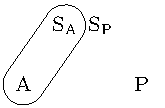
\includegraphics[\width=\linewidth]{figures/alignment}
Participant indexing on verbs thus displays split-intransitive alignment: active verbs index transitive and intransitive subjects identically while distinguishing objects (\ref{ex:alignment1}, \ref{ex:alignment2}). Stative verbs do not index their invariably intransitive subject like active verbs do (\ref{ex:alignment3}), nor do their suffixes overlap with undergoer marking on transitive verbs (\ref{ex:alignment1}). An illustration is given in \Cref{fig:verb_alignment}.

\is{Alignment}
\begin{figure}
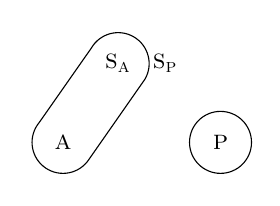
\begin{tikzpicture}
	\topnode{}
	\topleftnode[sa]{\gl{S\textsubscript{A}}}
	\toprightnode[sp]{\gl{S\textsubscript{P}}}
	\leftnode[a]{\gl{a}}
	\rightnode[p]{\gl{p}}
	\draw \convexpath{11.2pt}{a,sa};
	\draw (p) circle (11.2pt);
\end{tikzpicture}
% % 		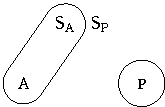
\includegraphics[width=0.3\linewidth]{figures/verb_alignment}
\caption{Verbal alignment}
\label{fig:verb_alignment}
\end{figure}


	\ea 
\label{ex:alignment1}
	\gll e=xhwii-ko\\
	 1\gl{sg}=bite-2\gl{sg}.\gl{obj} \\
	\glt \qu{I bite you.}
	\z
	
	
	\ea\label{ex:alignment2}
	\gll e=thana\\
	 1\gl{sg}=wander\\
	\glt \qu{I wander around.}
	\z
	
	
	\ea\label{ex:alignment3}
	\gll sinu-go\\
	 suffer-2\gl{sg}\\
	\glt \qu{You are ill, you suffer.}
	\z
	
	
	\ea\label{ex:WCstat_inan}
	\gll sinu (i=xh-ong)\\
	 suffer (\gl{def}.\gl{sg}=leg-1\gl{sg}.\gl{poss})\\
	\glt \qu{(My leg) hurts.}
	\z

The main types of verbs are the following.
\begin{enumerate}
	\item \emph{active transitive}: The subject marker precedes the verb (except in the imperative), and the verb takes an argument (see \sectref{ssec:TransV}); \textit{{e=xale-ke/ko}} \qu{I see it\slash you}.
	
	\item \emph{active intransitive}: The subject marker precedes the verb, the verb does not take an argument. \textit{{E=moo}} \qu{I stay}, \textit{a=yajen} \qu{it shakes, trembles}, \textit{a=temineen} \qu{it floats}. The productive transitive suffix \textit{-ke} and the older \textit{-i} can often be added to derive a transitive form (see \sectref{ssec:ke_i}).
	
	\item \emph{stative}: stative verbs are directly followed by their subject marker. The latter are bound to the verb stem and cannot choose their host, which is why I analyze them as suffixes rather than clitics; \textbf{\textit{me-o}} \qu{I die}. While the proclitic subject markers of active verbs are obligatory for all subjects, the stative subject markers are only obligatory for human arguments. They are almost, but not completely, identical to the object markers found on transitive active verbs with animate objects that are not expressed as noun phrases (see \Cref{tab:markers}). Stative verbs cover a few semantically defined, closed groups of words.
	\begin{itemize}
	\sloppy
		\item numerals (\textit{see-a} \qu{be.one-3\gl{sg}}, \textit{thaloo-lu} \qu{be.two-3\gl{du}}, \textit{thien-le} \qu{be.three-3\gl{sg}})
		\item semantically ``patientive" verbs like \textit{sinu-ong} \qu{suffer-1\gl{sg}} \qu{I am sick/ I suffer}, \textit{xhwiiti-o koo-n} \qu{long.after-1\gl{sg} \gl{obl}-3\gl{sg}} \qu{I miss it}
		%\item demonstratives \textit{ehni-o} \qu{this is me, here I am}
		\item \textit{heeve-o/-go/-a} \qu{where-1\gl{sg}/-2\gl{sg}/-3\gl{sg}} \qu{where am I/are you/is s/he}
		\item verbs with ``adjectival meanings" like \textit{vun-go} \qu{blue/green-2\gl{sg}} \qu{you are blue/green}, \textit{xhopwe-} \qu{(be) grow(n)}, \textit{mapehno-le} \qu{they are few}
	\end{itemize}
	\item There is also a group of verbs that cannot occur alone. They are not transitive, nor can they take subject markers, and they occur before or after another, independent, verb. These bound roots (called roots because they take no morphology on their own) are further described in \sectref{ssec:MannerV}.%, in things like \textit{vwa-thuan-ke} \qu{do-well-\textsc{tr}} looks like a compound.
\end{enumerate}

\section{Adverbs}
\is{Adverbs}
\label{sec:WCAdverbs}
Vamale possesses a small class of adverbs. They occur at the end of a clause or phrase, are frequently fronted without a phrase (\ref{ex:Adv}), take neither articles nor any kind of possessive or inflectional morphology, and are, if at all, modified by the intensifiers described in \sectref{sec:WCIntensifiers}, \textit{juu} \qu{real, really, very}. As they modify verb, noun, and prepositional phrases, and as they can be fronted alone, this analysis considers them to be adjuncts. Most members are transparently derived from nouns or prepositional phrases. See \sectref{sec:Adv} for examples of their interaction with verb and noun phrases. Example (\ref{ex:Adv}) features two cases of fronted adverbs,  (\ref{ex:Adv2}) shows an adverb at the end of a verb phrase, and (\ref{ex:Adv3}) shows an adverb after noun phrase.\largerpage[-2]

\ea
\label{ex:Adv}
(Adverbs are in bold, brackets show phrases, the comma separates two clauses)\\
\gll ka {\ob}jethro{\cb} \textbf{canbwen} man \textbf{bwethalo} {\ob}le=cuut cahni ka ni=bee-m-ca{\cb}, \textbf{cahni} {\ob}ca-n xhoogo{\cb}\\
 \gl{cnj} J. yesterday \gl{com} two.days.ago 3\gl{pl}=stand here \gl{sbj} \gl{def}.\gl{pl}=peer-2\gl{sg}.\gl{poss}-\gl{prox} here in-\gl{nspec} home\\
\glt \qu{And Jethro, yesterday and the day before your relatives stood here, here at home.} {[CP1:29]}
\z


\ea\label{ex:Adv2}
\gll e=ha-mwa \textbf{canbwen}\\
 1\gl{sg}=go-\gl{rep} yesterday\\
\glt \qu{I went back yesterday.} {[B2:134]}
\z


\ea\label{ex:Adv3}
\gll na i=vaaya-n xayu \textbf{habu} ka\\
 \gl{dem} \gl{def}.\gl{sg}=work-\gl{poss} man before \gl{disc}\\
\glt \qu{This was a man's work back then, like.} {[AG1:160]}\\
\z

\subsection{Temporal adverbs}
\label{ssec:TempAdv}

Temporal adverbs are a closed class of words that can occur in a fronted position (\ref{ex:tempadv}). They cannot take articles. Temporal adverbs were almost all derived from nominals, compare \textit{bwaabwen} \qu{morning} is related to the adverb \textit{bwaabwen-an} \qu{in the morning after}. Members include \textit{ca-n-bwen} \qu{yesterday (lit. \qu{in-\gl{nspec}-night})}, \textit{naen} \qu{today/now}, \textit{xahmaen} \qu{tomorrow}\footnote{Proto (Southern) Oceanic *marani \parencite[314]{lynch_efate-erromango_2004}.}, \textit{jimin} \qu{late at night (after having fallen asleep)}, \textit{bwethaloo} \qu{two days ago}, \textit{thaloobwen} \qu{overmorrow (lit. `two nights')}, \textit{daboo-n bwen} \qu{midnight (`lit. puddle/lake of the night')} %19-07-18, page 34)
\textit{hnyanan} \qu{constantly (lit. `its breath')}, \textit{mati} \qu{earlier}, \textit{mu-bwen} \qu{early in the morning (lit. `little night')}, \textit{nyeet} \qu{when?}, \textit{ca-li-been} \qu{sometimes (lit. `among the others')}. 

\ea \label{ex:tempadv}
\gll na li=\textit{peintures} habu\\
 \gl{dem} \gl{def}.\gl{pl}=paint before\\
\glt \qu{It's the (style of) painting from the old days.} {[KG:21]}
\z

\subsection{Locative adverbs}
\label{ssec:WCLocAdv}
A closed class of words describes locations. They are mostly derived from movement verbs.\footnote{\textit{Patemwano} \qu{directly next to it}, \textit{ngangeno} \qu{close-by} in Pije \parencite[170]{haudricourt_dictionnaire_1982} and \textit{puput} \qu{behind (a building or a sizeable entity)} can be used in the same slots but do not possess the morphological combinatorics shown in \Cref{tab:LocAdv}.} They do not bear articles, can be fronted alone (\ref{ex:front_xahut}), and can modify verbs (\ref{ex:xahut1}) as well as nouns (\ref{ex:LocAdvPred}). Locative adverbs can be predicates, see (\ref{ex:LocAdvPred}). Contrary to relational nouns (\sectref{ssec:WCPrepoNouns}), locative adverbs do not form possessive relations with nouns, nor do they take generic \textit{-n}. \Cref{tab:LocAdv} shows a summary of the forms. For a more thorough account of space (see \sectref{ssec:spat_adv}).
%members: (\textit{xahan}, \textit{xahut}, \textit{xada}, \textit{xahnuut}, \textit{xahnuda}, \textit{nya-xahan} etc, possibly \textit{patemwano}

\begin{table}
	\caption{Locative adverbs}
	\fittable{\begin{tabular}{lllll}
		\lsptoprule
	                &      & Simple & \\
		Axis		& Verb & location & Close-by& Further away\\
		\midrule
		same-level& \textit{han}& \textit{xa-han}& \textit{nya-xa-han} & \textit{nya-an xa-han}\\
		downward & \textit{hut}& \textit{xa-hut} & \textit{nya-xa-hut} & \textit{nya-ut xa-hut}\\
		upward & \textit{ta} &	\textit{xa-da} & \textit{nya-xa-da} & \textit{nya-da xa-da} \\
		downstream & \textit{hnuut}& \textit{xa-hnuut}& \textit{nya-xa-hnuut} & \textit{nya-hnut xa-hnuut}\\
		upstream & \textit{hnuuda} & \textit{xa-hnuuda} & \textit{nya-xa-hnuuda}& \textit{nya-hnuda xa-hnuuda}\\
		\lspbottomrule
	\end{tabular}}
\label{tab:LocAdv}
\end{table}


\ea\label{ex:xahut1}
\gll go=moo xahut, go=xahut, go=hut xahut\\
 2\gl{sg}=stay below 2\gl{sg}=below 2\gl{sg}=go.down below\\
\glt \qu{You live down there, you're down there, you go down there.}
\z


\ea\label{ex:front_xahut}
\gll xahut, go=majit mati\\
 below 2\gl{sg}=rest earlier\\
\glt \qu{Down there, you were sleeping earlier.}
\z


\ea\label{ex:LocAdvPred}
\gll i=apuli (a=) xahut\\
 \gl{def}.\gl{sg}=man (3\gl{sg}=) below\\
\glt \qu{The man is down there.}
\z

\subsection{\textit{hman} \qu{also}}
\textit{hman} \qu{also} modifies verbs (\ref{ex:hmanV}), nouns (\ref{ex:hman}), and adverbs. Contrary to temporal and locative adverbs, \textit{hman} always comes after the modified word and cannot be fronted on its own. Similarly to \textit{mwa} (\sectref{sec:mwa}), \textit{hman} is used as a discourse marker as well, with a meaning of \qu{however} (\ref{ex:hmanDisc}).

\ea\label{ex:hmanV}
\gll tha gau=han tha gau tha gase=bo \textit{arriver} hman\\
 \gl{ass} 2\gl{du}=go \gl{ass} 2\gl{du} \gl{ass} 1\gl{pl}.\gl{incl}=\gl{irr} arrive also\\
\glt \qu{You go (despite the height of the steel beam), you two, we'll get (to the other side), too.} {[KG:9]}
\z

\ea\label{ex:hman}
\gll li=meeka i=\ldots  li=nyan-mwa ca-n {hman}\\
 \gl{def}.\gl{pl}=all \gl{def}.\gl{sg}=\ldots \gl{def}.\gl{pl}=inside-house in-\gl{ana} also\\
\glt \qu{All the rooms in the house as well.} {[KG: 30-1]}
\z

\ea\label{ex:hmanDisc}
\gll thake yavo kavi tha cipa xhwii hman\\
 throw fishing.line but \gl{ass} \gl{neg} bite also\\
\glt \qu{...threw out the fishing line but it didn't bite though.} {[GP:73]}
\z

\section{Complementizer \textit{hapi}}
\is{Subordination!Complementation}
Clauses that are complement to verbs of cognition (\ref{ex:hapi2}), opinion, and perception (\ref{ex:hapi3}), are introduced by the subordinator \textit{hapi}. Considering \textcite{lynch_oceanic_2002}'s observation that Oceanic languages tend to use a form related or identical to the word \qu{to say} to introduce complement clauses \parencite[53]{lynch_oceanic_2002}, that Voh-Koné languages changed \textit{p-} $\rightarrow$ \textit{v-}, and that Hienghène languages have \textit{peei} \qu{to say}, \qu{\gl{comp}} \parencite[260]{haudricourt_dictionnaire_1982}, postulating \textit{a=vii} \qu{s/he says} as the origin of \textit{hapi} seems plausible.


\ea\label{ex:hapi2}
\gll e=caihna-n hapi tha hmwaana\\
 1\gl{sg}=know-\gl{nspec} \gl{comp} \gl{ass} thus\\
\glt \qu{I know that it's like that.}
\z


\ea\label{ex:hapi3}
\gll sahnaang-eong hapi tha hmwaana\\
 not.understand-1\gl{sg} \gl{comp} \gl{ass} thus\\
\glt \qu{I'm not sure/I doubt that it's like that.}
\z

\section{Conjunctions}
\label{sec:Conj}
Vamale distinguishes two groups of conjunctions: those that link noun phrases, and those that link verb phrases as well as clauses. Clauses are defined by the presence of a predicate, which is in most cases a verb phrase. This book calls the conjunctions linking these ``verbal", to distinguish them from nominal ones.   

\subsection{Nominal conjunctions}
\label{ssec:NomConj}

Nominal conjunctions connect noun (phrases) and form a new constituent containing the connected noun phrases and the conjunction. Members include \textit{ma} `and\slash with' (\ref{ex:maconj}), \textit{ka} `on the other hand' (\ref{ex:kaconj}), \textit{hai} \textasciitilde \textit{a} \qu{or} (\ref{ex:haiconj1}) with its derivative \textit{hai...hai} \qu{either...or} (\ref{ex:haiconj}),  \textit{moko} \qu{more than}. \textit{Moko} may be complex and composed of \textit{moo} \qu{rest, reside} and \textit{ko} \qu{on} (\sectref{sec:Comp}). It has no Hienghène cognate. The other Voh-Koné varieties share the form, however. \citet[215]{rivierre_bwatoo_2006} suggest a makeup of \textit{mo} \qu{from}, as in \textit{e ha-me \textbf{mo} Tuo} \qu{I come \textbf{from} Touho}, and \textit{ko} \qu{on}. 


\ea\label{ex:maconj}
\gll i=wabatan ma i=xat\\
 \gl{def}.\gl{sg}=north.wind and \gl{def}.\gl{sg}=sun\\
\glt `the north wind and the sun'
\z


\ea\label{ex:kaconj}
\gll i=wabatan ka i=xat\\
 \gl{def}.\gl{sg}=north.wind and \gl{def}.\gl{sg}=sun\\
\glt `the north wind, and (on the other hand) the sun'
\z


\ea\label{ex:haiconj1}
\gll i=wabatan hai i=xat\\
 \gl{def}.\gl{sg}=north.wind or \gl{def}.\gl{sg}=sun\\
\glt`the north wind or the sun'
\z


\ea\label{ex:haiconj}
\gll hai i=wabatan hai i=xat\\
 or \gl{def}.\gl{sg}=north.wind or \gl{def}.\gl{sg}=sun\\
\glt \qu{either the north wind or the sun}
\z

\subsection{Verbal conjunctions}
\label{ssec:VerbConj}

\is{Coordination!Verbal conjunctions}
The set of verbal conjunctions is small and closed, and groups together some morphemes which only occur in this set, like \textit{kavi} \qu{but}, with words also present in other distributional classes. The meaning distinctions between \textit{kavi} \qu{but (introducing something in contrast with the former element)}, \textit{ko} \qu{but [introducing something unexpected)}, and \textit{ma} \qu{but (relaying something related but different)} are fine and depend on the context. Members include \textit{ka} `and' (\ref{ex:kaVC}), \textit{kavi} `but' (\ref{ex:kaviVC}), \textit{ma} `and, but' (\ref{ex:maVC}), \textit{hai} \goodtilde \textit{a} `or' (\ref{ex:haiVC}), \textit{ko} \qu{but}, \qu{because}, \textit{kona} \qu{furthermore}. 


\ea\label{ex:kaVC}
\gll le=hame ka le=siwa=mwa\\
 3\gl{pl}=come and 3\gl{pl}=return=\gl{rep}\\
\glt `They came and they left again.'
\z


\ea\label{ex:kaviVC}
\gll le=hame kavi le=siwa-mwa\\
 3\gl{pl}=come but 3\gl{pl}=return-\gl{rep}\\
\glt `They came but they left again.'
\z


\ea\label{ex:maVC}
\gll le=ha-me ma le=siwa-mwa\\
 3\gl{pl}=go-\gl{dir.cp} and 3\gl{pl}=return-\gl{rep}\\
\glt `They come and/in order to go.'
\z


\ea\label{ex:haiVC}
\gll le=ha-me hai le=siwa=mwa\\
 3\gl{pl}=go-\gl{dir.cp} or 3\gl{pl}=return=\gl{rep}\\
\glt `They come or they go.'
\z

\textit{Ka} is also used colloquially after a clause to ask for confirmation (\ref{ex:kaDisc}) (see \sectref{discourse ka}).

\ea \label{ex:kaDisc}
\gll i=apuli a=xahan ka?\\
 \gl{def}.\gl{sg}=person \gl{rel}=over.there \gl{disc}\\
\glt \qu{The guy over there, like?}
\z

%\subsubsection{Numeral coordinators \textit{na-bwa}, \textit{ko}}
\is{Coordination!Numeral coordinators}
Numbers are verbal, and \textit{(na)-bwa} \qu{plus} (possibly from \gl{dem}-\qu{head}, \ref{ex:nabwa}), and \textit{ko} \qu{times} (probably from \textit{ko} \qu{on}) are used to construct complex numbers (\ref{ex:nabwako}). 


\ea\label{ex:nabwa}
(nim a-bwa se)\\
\gll nim na-bwa se\\
 5 plus 1\\
\glt \qu{6}
\z


\ea\label{ex:nabwako}
\gll nim na-bwa se ko apuli nabwa nim na-bwa se\\
  5 plus 1 times man/20 plus 5 plus 1\\
\glt \qu{126}
\z

\section{Subordinators}

Vamale subordinators introduce a subordinated clause. They precede all other elements of said clause, and cannot occur without the clause, moving with it if fronted, see examples (\ref{ex:fronted}--\ref{ex:frontedend}). All those ending on -\textit{a} assimilate to following \textit{e=} \qu{1\gl{sg}}. They are proclitics.
Members include \textit{cala} `when' \textit{cama} `if', \textit{ma} `as\slash in order to', \textit{ko} `because', \textit{ko-ma} `so that',  \textit{ecupwa}  \qu{until}.\footnote{Possibly from \textit{e-cuut-pwa} \qu{\gl{refl}-stand-on}.}

\ea \label{ex:fronted}
\gll cel=e=hame go=pa yahan\\
 when=1\gl{sg}=come 2\gl{sg}=\gl{prf} leave\\
\glt `When I came, you had already left.'
\z


\ea
\gll cala go=hame e=pa yahan\\
 when 2\gl{sg}=come 1\gl{sg}=\gl{prf} leave\\
\glt `When you came, I had already left.'
\z


\ea
\gll cem=e hame go=pa yahan\\
 if/when=1\gl{sg} come 2\gl{sg}=\gl{prf} leave\\
\glt `If I come, you will already have left.' \\'Whenever I come, you already have left.'
\z


\ea
\gll cama go=hame e=pa yahan\\
 if/when 2\gl{sg}=come 1\gl{sg}=\gl{prf} leave\\
\glt `If you come, I will already have left.' \\ `Whenever you come, I already have left'
\z


\ea
\gll m=e hame go=pa yahan\\
 as=1\gl{sg} come 2\gl{sg}=\gl{prf} leave\\
\glt `As I come, you've already left.'
\z


\ea \label{ex:frontedend}
\gll ma le=fe, le=mu=xaahni\\
 as 3\gl{sg}=take, 3\gl{pl}=\gl{freq}=check\\
\glt \qu{When they take it, they check it.}
\z

Non-fronted examples, illustrated in (\ref{ex:non-fronted}), are the norm.

\ea \label{ex:non-fronted}
\gll tha=abe=saavi cama=abe icu-koo-n ko-n \textit{marché}\\
 \gl{ass}=1\gl{pl}.\gl{excl}=dig.up \gl{subr}=1\gl{pl}.\gl{excl} trade-\gl{obl}-\gl{ana} on-\gl{nspec} market\\
\glt `We dig (them) up when we sell them on the market.' {[AG1:22]}
\z


\ea
\gll le=thêên cala le=siwa-mwa\\
 3\gl{pl}=run when.\gl{real} 3\gl{pl}=return-\gl{rep}\\
\glt \qu{They ran when they went back.}
\z

\ea
\gll le=thêên ma le=yahan\\
  3\gl{pl}=run when.\gl{irr}/if 3\gl{pl}=leave\\
\glt `(Usually) they run when they leave.' / `They would run if they left.'
\z


\ea
\gll e=ha-me ma go=bwa=yahan\\
 1\gl{sg}=go-\gl{dir.cp} \gl{subr} 2\gl{sg}=\gl{ipfv}=leave\\
\glt `I come as as you leave.' / `I come if you leave.' / `I come so that you leave.'
%\a
%
%\gll le=ɣahni ma le=fe
%
% 3\gl{pl}=check in.order.to 3\gl{pl}=take
%
%\glt \qu{they're checking to take}
%
%
\z




\section{Negation markers}
\is{Negation}

The negation markers \textit{cipa} \qu{\gl{neg}} and \textit{cipii} \qu{\gl{proh}} share their scope over the entire following clause and their left-most position. The negation markers are not identical in their distribution and could, strictly speaking, be classified into two separate classes. Contrary to \textit{cipa} \qu{\gl{neg}} (\ref{ex:thacipa}), \textit{cipii} \qu{\gl{proh}} cannot take assertive \textit{tha}, nor \textit{na} \qu{\gl{foc}}. Furthermore, \textit{cipii} often omits the subject marker, which \textit{cipa} cannot do (\ref{ex:cipi}). This grammar will treat \textit{cipa} as a proclitic, because it integrates into the following verb phrase's stress structure, and assimilates phonologically to it as well (\ref{ex:cipa}).
%

	
	\ea\label{ex:thacipa}
	\gll (tha) cipa {\ob}go=bwaa=majit{\cb}?\\
	 (\gl{ass}) \gl{neg} 2\gl{sg}=\gl{ipfv}=sleep\\
	\glt \qu{Aren't you still asleep?}
	\z
	
	
	\ea\label{ex:cipa}
	[ˌci.pe.ˈmãn.ɟit]\\
	\gll cipa= e= majit\\
	 \gl{neg} 1\gl{sg}= sleep\\
	\glt \qu{I don't sleep.}
	\z
	
\ea \label{ex:cipi}
\gll cipii xaloo koo-ng hmwaahni (ka go)! \\
 \gl{proh} gaze \gl{obl}-1\gl{sg}.\gl{poss} thus \gl{sbj} 2\gl{sg}\\
\glt \qu{Don't look at me like that!}
\z

\section{Assertive \textit{tha}}
\label{sec:WCAssertive}
\is{Assertive \textit{tha}}

The assertive marker \textit{tha} is a proclitic that docks onto the predicates of non-imperative clauses, on the left-most position (\ref{ex:tha1}). \textit{Tha} assimilates to \textit{e=} \qu{1\gl{sg}}, like \textit{cipa} \qu{\gl{neg}} (\ref{ex:tha2}). %unlike \textit{na} \qu{\gl{dem}}, pro-clitic to predicates.



\begin{exe}[(999)]
\ex \label{ex:tha1}
\gll \textit{au lieu} ma tha bwa xhavwale i=\textit{copain}-ea vukin tha=a bo \textit{guide}-ea\\
 instead \gl{subr} \gl{ass} \gl{ipfv} wait \gl{def}.\gl{sg}=friend-3\gl{sg}.\gl{poss} reason \gl{ass}=3\gl{sg} \gl{irr} guide-3\gl{sg}.\gl{poss}\\
\glt \qu{Instead of waiting for his friend, because he would be his guide!} {[KG:497]}
\end{exe}


\ea\label{ex:tha2}
\gll cala th=e vwa-tau \\
 when \gl{ass}=1\gl{sg} do-impact\\
\glt \qu{when I fish} {[B3:3]}
\z

\section{Intensifiers}
\label{sec:WCIntensifiers}
\is{Intensifiers}

The two intensifiers \textit{juu} \qu{real, very} and \textit{vaa} \qu{(too) much} (most often preceded by \textit{juu}, but see \ref{ex:vaa}) cannot stand alone, are semantically vague (see \Cref{tab:juu}), and attach to the head of a phrase (be that a noun, an adverb, or anything else, \ref{ex:juu}) as closely as possible. Given that they can be stressed, they are analyzed as particles, though ``anti-clitic" may be a better term considering the fact that they syntactically depend on a host that can be nominal, verbal, or adverbial in nature. \textit{Juu} is also associated to \textit{bwa} \qu{\gl{ipfv}}, as described in \sectref{ssec:bwa_ju}.


\ea\label{ex:juu}
\gll a=juu hnyimake ka i=juu apuli, juu ca-n-bwen\\
 3\gl{sg}=very think \gl{sbj} \gl{def}.\gl{sg}=real person real in-\gl{nspec}-night\\
\glt `He thought hard, the real man, just yesterday.'
\z


\ea\label{ex:vaa}
\gll ma go=hmwaani vwasoon, ma go=hmwaani vaa...\\
 \gl{cond} 2\gl{sg}=like.this impossible \gl{cond} 2\gl{sg}=like.this too.much\\
\glt \qu{If you do it like this, it's impossible, and if you do it like this, it's too...} {[KG:140]}
%\a
%
%\gll na li=a le=ɣaleke
%
% DEM.PRED SPEC.PL REL 3PL=see
%
%\glt `It is they who watched.'
%
%
\z


\begin{table}
	\caption{Meanings of compounds with \textit{juu}}
	\begin{tabular}{lll}
	\lsptoprule
		Form & \multicolumn{2}{c}{Translation of}\\\cmidrule(lr){2-3}
		     & the 2nd morpheme & the whole\\
	\midrule
		\textit{juu han} & walk & \qu{walk barefoot}\\
		\textit{juu aman} & thing & \qu{important (adverb)}\\
		\textit{juu we} & water & \qu{drinking water} \\
		\textit{juu toot} & grass & \qu{thatching grass}\\
		\textit{juu o} & bamboo & \qu{building bamboo}\\
		\textit{juu mwa} & house & \qu{trad. house}\\
		\textit{juu mani} & bird & \qu{{notou} {[ducula goliath]}}\\
		\textit{juu apuli} & person & \qu{Kanak}\\
		\textit{juujuu} & & \qu{truth}\\
	\lspbottomrule
	\end{tabular}
\label{tab:juu}
\end{table}

The particle \textit{vaa}, depending on the word it modifies, means \qu{much (uncountable)} with non-human nouns (\ref{ex:vaa1}), %meaning \qu{many} for ants, in contrast to \textit{hmain}, \qu{many} for humans.
 intensifies the following verb, e.g. \textit{vaa thêên} \qu{strongly run}\slash\qu{run fast}, and in combination with \textit{ju} \qu{real, true}, it means \qu{too much}, as in (\ref{ex:vaa2}). 


\ea\label{ex:vaa1}
\gll e-vaa nya-da xa-da\\
 \gl{mid}-\gl{ints} towards-up.there \gl{loc}.\gl{adv}-up \\
\glt \qu{There are many (feral pigs) up there.} {[J3 16.1]}
\z


\ea \label{ex:vaa2}
\gll juu va vwasoon ma gase=vwa li=vaaya-n li=xhaohmu\\
 real much difficult \gl{comp} 1\gl{pl}.\gl{incl}=do \gl{def}.\gl{pl}=work-\gl{poss} \gl{def}.\gl{pl}=elder\\
\glt \qu{It's too hard for us to do the work of the elders.} {[KP:98]}
\z



\section{Repetitive \textit{mwa}}
\label{sec:WCRepetitive}
\is{Repetitive \textit{mwa}}

This class only has one member. \textit{Mwa} has rather different, related meanings, depending on the context. \textit{Mwa} can have the repetitive meaning \qu{again} (\ref{ex:mwa_even}), the restitutive \qu{back}, as well as \qu{also}, \qu{even}, \qu{on top of that}, or mark the preceding phrase as focused (see \sectref{sec:mwa} for a discussion). The deictic use of \textit{mwa} \qu{now} (\ref{ex:mwa}), seems to mostly anchor the listener's attention, similarly to \textit{mwa} \qu{even}, onto the noun phrase given, see (\ref{ex:mwa_now1a}). \textit{Mwa} is a particle that can dock onto any phrase preceding it (see \ref{ex:mwa_rep}).

\ea\label{ex:mwa_even}
\gll e=xaleke mwa\\
 1\gl{sg}=see \gl{rep}\\
\glt `I see again.', `I even see.'
\z

\ea
\label{ex:mwa_rep}
\gll e=vatipwe mwa nya-mwa si-m mwa i=mwani mwa\\
 1\gl{sg}=drop \gl{rep} give-\gl{rep} hand-2\gl{sg}.\gl{poss} \gl{rep} \gl{def}.\gl{sg}=money \gl{rep}\\
\glt \qu{I pass on to you too this money as well.}
\z


\ea\label{ex:mwa}
\gll hê na tha vwa li=wii-n. go le=vwa ibi-han li=nyamaan go tha le=ve-moo mwa, moo mwa. \\
 yes \gl{dem} \gl{ass} \gl{exist} \gl{def}.\gl{pl}=field-\gl{poss}.\gl{nspec} then 3\gl{pl}=do pinch-walk \gl{def}.\gl{pl}=eye then \gl{ass} 3\gl{pl}=\gl{mid}-stay \gl{rep} stay \gl{rep}\\
\glt \qu{Yes there were fields of it (macaranga vedeliana). And they'd go pinch the young sprouts. And those stay together now, stay.} {[KL:218-222]}
\z


\ea\label{ex:mwa_now1a}
\gll ya a=ja vwa \textbf{mwa} li=wee-n a=ta-\textbf{mwa} sibu li=sibu \textbf{mwa}. ja yabwat \textbf{mwa} sisuu \textbf{mwa}\\
 \gl{expl} 3\gl{sg}=\gl{prf} do \gl{rep} \gl{def}.\gl{pl}=water-\gl{poss}.\gl{nspec} 3\gl{sg}=go.up-\gl{rep} swell \gl{def}.\gl{pl}=swell \gl{rep} \gl{prf} dry \gl{rep} hard \gl{deict}\\
\glt \qu{And there's the sap that rises, swells, the swells there. It dries then, gets hard then.}
\z

In (\ref{ex:movV-mwa1}) and for all other movement verbs, as well as \textit{xhose} \qu{do again}, \textit{mwa} is analyzed as a suffix, i.e. as having fused with its host. First, \textit{mwa} assimilates to the root, which it does not do in other contexts.\footnote{\textit{Xhosepwa} suggests a dropped \textit{-t} or \textit{-p}. The Pije and Fwâi cognates \textit{khô-peei} \qu{?-say} \parencite[155]{haudricourt_dictionnaire_1982} could be a diachronic hint at a morphologically complex, old Vamale form.} Compare \textit{hut-mwa} $\rightarrow$ /hupʷa/ \qu{go back down}, to \textit{hut=mwa} \qu{go down again}.

%\begin{multicols}{2}
\ea \label{ex:movV-mwa1}
\gll go=ha-mwa-me\\
 2\gl{sg}=go=\gl{rep}=\gl{dir.cp}\\
\glt \qu{You return to me, you come back.}
\z


\ea
\gll go=ha-me mwa\\
 2\gl{sg}=go=\gl{dir.cp} \gl{rep}\\
\glt \qu{You come again.}
\z
%\end{multicols}

The particle also expresses repetition (\ref{ex:mwa_rep1a}), and deictically referring to something close spatially or recently mentioned (which is probably a derived meaning), as in (\ref{ex:mwa_rep1b}). See \sectref{sec:mwa} for a more detailed description. %Also means "even, on top of that". 


\ea\label{ex:mwa_rep1a}    
\gll e=tena mwa\textsuperscript{{\upshape REP}} i=hun-det\\
 1\gl{sg}=hear \gl{rep} \gl{def}.\gl{sg}=\gl{nmlz}-sound\\
\glt \qu{I hear the sound again.} {[JR:17]}
\z

\ea\label{ex:mwa_rep1b}
\gll xhose e=tena mwa\textsuperscript{{\upshape REP}} tha=a=bwa vwa det mwa\textsuperscript{{\upshape\gl{deict}}}\\
 again 1\gl{sg}-feel \gl{rep} \gl{ass}=3\gl{sg}=\gl{ipfv} do sound \gl{rep}\\
\glt \qu{Again I heard him make said (\textit{mwa}) noise.} {[JR:18]}
\z 


%intransitive und transitive stämme in vamale müssen nicht postuliert werden, bzw. kein unterschied zu intransitiven und transitiven wurzeln

\section{Interjections}
\is{Interjections}
Interjections do not integrate into clauses or phrases, and though at least \textit{hê} \qu{yes} can be derived to \textit{hêêke} \qu{to assent, to say yes}, and \textit{cika} \qu{\gl{neg}.\gl{exist}} is a commonly used impersonal verb, exclamations form a group through their uniquely individualistic behavior.
Members include \textit{ya} \qu{voilà, the result is there}, \textit{ûhû}\slash\textit{cika} \qu{no}, \textit{hat} \qu{strong negation}, \textit{hai} \qu{oh! (surprise, discovery)} and \textit{hê}\slash\textit{helong} \qu{yes}, as well as a growing class of swearwords. 

\section{Quantifiers}
\is{Noun phrase!Quantifiers}
Quantifiers are a tiny group of particles that are not inflected, directly preceding an (article) noun construction: \textit{mu} \qu{little}, \textit{jaa} \qu{many} (\ref{ex:jaa}), and \textit{ju-vaa} \qu{too much}, which is also attested as an intensifier in verb phrases (\ref{ex:juva}). Quantifiers denote number and are described in \sectref{ssec:Quant}. Other words have similar meanings, but are verbs, like \textit{hmai-} \qu{many}. One quantifier similarly integrates the noun phrase, but bears possessive suffixes: \textit{meeka-n} \qu{all}.



	\ea\label{ex:jaa}
	\gll ja apuli canbwen\\
	 many people yesterday\\
	\glt \qu{(there were) more people yesterday (than now)} {[B2 31.1]}
\z	
	
	\ea\label{ex:juva}
	\gll ju-vaa apuli\\
	 too.much person\\
	\glt \qu{too many people} {[B2:32]}
	\z
	


%\section{Conclusion}
%Does it even need to have a conclusion?
%\begin{quote}
%	Vamale wordos:\\
%	They differ like spring flowers\\
%	Behold the garden.\\
%\end{quote}
%\begin{table}
%\begin{tabular}{p{3cm}|c|c|c|c|c|c}
%takes / appears in & nouns & \multicolumn{2}{c}{verbs} & adverbs & \\
%\midrule
%&& active& stative&&&\\
%\midrule
%Articles & x &&&&&\\
%Possessive suffixes& x &&&& &\\
%S/A- markers and -O markers&  & x&&&&\\
%-S markers& && x&&&\\
%in NP& x &&& x& &\\
%in VP&& x& x&& x&\\
%\end{tabular}
%\caption{Word classes}
%\label{tab:WordClasses}
%\end{table}

% i want this section to say how i work and why, and what problems and particularities i encountered in the field. 
\chapter{Nouns} 
\label{ChapterNouns} 
\is{Nouns}

Vamale nouns are defined in this grammar as single words which can bear articles (see \sectref{sec:WCArticles}). Few other factors distinguish nouns from verbs, as nouns can be predicates with the same subject index markers as active verbs, see (\ref{ex:e-caacaa}). Only nouns, however, can be arguments of verbs, can be counted, can be possessed (though possessive morphology shows overlaps with some verbal morphology (see \sectref{sec:StatV} and \sectref{ssec:PossV}), and not all nouns can be possessed, e.g. \textit{jati} \qu{sea}). Although nouns do take some TAM marking, not all TAM marking is attested for nouns (e.g. \textit{bwa balan} \qu{only just (begun)}, \textit{kon} \qu{\gl{prog}}). Nouns are not inflected for number; this is covered by articles (for specific nouns; generic ones do not have articles).

	\ea 
	\label{ex:e-caacaa}
	\gll e=juura caacaa\\
	 1\gl{sg}=almost father\\
	\glt \qu{I am almost a father (soon).} {[B2:108]}
	 \z
	
	\ea
	\gll xhwat thuang m=e=caacaa\\
	 bit joke \gl{subr}=1\gl{sg}=father\\
	\glt \qu{I am almost a father (kind of).}
	\z

%Untergruppe: inalienable Nomina müssen besessen werden, im Notfall von 3\gl{sg} (falls -\textit{n} 3\gl{sg} darstellt, und 3\gl{sg} nicht -n-0 ist). Dies wird entweder mit den Possessivpronomen gekennzeichnet oder mit der Possessor-NP nach dem Verb.

\begin{sloppypar}
Vamale nouns can be classified along different dimensions. The animate\slash inanimate distinction, a semantic, lexically determined trait, affects their index\hyp marking on verbs. While index\hyp marking is treated in \sectref{ssec:TransV}, other effects of this distinction are described in \sectref{sec:animN}. Some nouns are uncountable (such as water, light, blood, etc.) and are thus not attested with non-singular articles. %and their syntactic origin (\Cref{sec:NomDeriv}). 
Finally, possessible nouns can be either alienably or inalienably possessed. This distinction is another typically Oceanic feature \parencite[41]{lynch_oceanic_2002}, though Vamale has added its own innovations (see \sectref{sec:Poss}). This chapter will briefly introduce these dimensions, but will focus only on possession, as the others are lexically determined. 
This chapter will also discuss classifiers (\sectref{sec:CL}). Vamale does not have many classifiers, and they are mostly relational: they add information about the nature of relationship between the possessor and the possessum. An exception are food classifiers, which, contrary to the possessive classifiers, can appear without the noun they classify. \sectref{ssec:NounCL} describes noun classifiers, which are obligatory in the context of plant species: \textit{mwago} \qu{mango} cannot appear alone; one must specify which part of the plant is meant. Noun classifiers are related to a much larger field of optional noun compound heads. Compound nouns are discussed in \sectref{sec:CompN}.
\end{sloppypar}

\section{Animacy}
\label{sec:animN}
\is{Animacy}

Nouns in Vamale are animate or inanimate. While other languages in New Caledonia distinguish human and non-human animate nouns (Cèmuhî even makes a difference between feminine and non-feminine nouns, \citealt[175]{rivierre_langue_1980}), this is of no importance in Vamale. An exception are some nouns, e.g. \textit{in maan} \qu{skin (human)} vs. \textit{in} \qu{skin (non-human, or dead human)}, and oblique markers:  \textit{nyasi-} \qu{\gl{ben}, \gl{top}} can only be used for humans whereas \textit{nyako-} is more general (see \sectref{sec:oblique}). %and the spatial prepositions \textit{puput} \qu{behind (inanim. subject)} and \textit{cai-} \qu{behind (anim. subject)} are for inanimate, and animate, nouns, respectively. 
Animate participants further trigger person marking on stative verbs (\ref{ex:animNstV}) and must be indexed with suffixes on transitive verbs (\ref{ex:animNOBJ}). Both contexts omit any indexing if the relevant noun phrase occurs within the verb phrase (\ref{ex:animNinVP}). 


	\ea\label{ex:animNstV}
	\gll ka abe niehni a= \textbf{thien-abe}\\	
	 \gl{cnj} 1\gl{pl}.\gl{excl} \gl{dem}.\gl{pl} \gl{rel}= three-1\gl{pl}.\gl{excl}\\
	\glt \qu{And we are those [masters of the rock], who are three (and we are these three masters of the rock).} {[DP:29]}
	\z
	
	
	\ea\label{ex:animNOBJ}
	\gll na cahni tha xhwan see-a a= thathe-\textbf{a}\\	
	 \gl{dem} here \gl{ass} a.bit one-3\gl{sg} \gl{rel}= kill-3\gl{sg}.\gl{obj}\\
	\glt \qu{Here there was only one that was killed.} {[HC1:22]}
	\z
	


\ea \label{ex:animNinVP}
(\textit{hmwet} is a stative verb)\\
\gll hmwet i=apuli\\
 tired \gl{def}.\gl{sg}=person\\
\glt \qu{The person is tired.} {[J8:7]}
\z

Another context in which animacy makes a difference is deverbal nominalizations, in which case the intransitive subject is only marked for person if the referent is animate: \textit{i hun-moo-a} \qu{\gl{def}.\gl{sg}=\gl{nmlz}-be-3\gl{sg}} \qu{his/her character}, but \textit{i hun-moo} \qu{its nature}. This is described in more detail in \sectref{sec:NomDeriv}.
\section{Possession}
\label{sec:Poss}
\is{Possession}

Possessed nouns make a distinction in alienability, i.e. whether they can occur without marking a possessor. This is a widespread Oceanic phenomenon \parencite[511]{ross_morphosyntactic_2004}. Alienable and inalienable nouns follow certain semantic tendencies outlined in Table \ref{tab:semantic_poss}, though there are numerous exceptions. Non-possessible nouns include proper names and unique concepts such as the sea or the sun, although poetic contexts may feature counterevidence. Another exception is \textit{la} \qu{place}, which can neither be generic (as would be indicated by \textit{-n} on preceding verbs and prepositions), nor take an article, but syntactically behaves like a noun otherwise (i.e. it follows prepositions) (\ref{ex:la}).

\ea \label{ex:la}
\gll suu cahni ca la\\
 break here in place\\
\glt \qu{Break it here at this spot!} {[KG:115]}
\z 

\begin{table}
	\caption{Semantic tendencies of possessed nouns}
	\begin{tabular}{ll}
		\lsptoprule
		Inalienable&	Alienable\\
		\midrule
		Body parts (except blood)&	Animals\\
		Things belonging to humans &	Plants\\
		(spirit, colour, appearance, strength)&\\
		Many kinship appelation terms (not the address forms)&	Tools\\
		\lspbottomrule
	\end{tabular}
\label{tab:semantic_poss}
\end{table}

\begin{sloppypar}
However, while most Oceanic languages distinguish direct (i.e. affixed) possession from indirect constructions using a relational classifier, Vamale has mostly done away with this distinction. Based on prosodic clues, especially stress shift, all possessive morphemes are considered suffixes, as in [ˈpu.a.ka] \qu{pig}, [pu.a.ˈka.ne.ɔŋ]\slash [pu.a.ˈka.ne.o] \qu{my pig}. The only clearly indirect possessive morpheme remaining is the linker \textit{ka-}, discussed in \sectref{kan}.
Possessive forms are not a sure sign of the nounhood of their host, even though nouns represent the vast majority of possessed lexemes. There are verbs with nominal morphology (e.g. \textit{hmana-n} \qu{hunger-3\gl{sg}.\gl{poss}, s/he is hungry}), and some stative verbs that have an identical nominal counterpart, e.g. \textit{mulip, muliv-ong} \qu{life, I am alive} (see \sectref{sec:WCVerbs} and \sectref{ssec:PossV}).
\end{sloppypar}

%\begin{table}
%	\parbox{0.45\linewidth}{
%		\centering
%		\caption{Alienable possessive suffixes (sometimes length changes: \textit{nya+ko+n} = \textit{nyakoon})}
%		\begin{tabular}{l|llll}
%			&	1&	1+&	2&	3\item
%			SG&		\multicolumn{2}{c}{eong}&		go&	ea\item
%			DU&	abu&	gasu&	gau&	lu\item
%			PL&	abe&	gase&	gavwe&	le\item
%		\end{tabular}
%	}
%	\hfill
%	\parbox{0.45\linewidth}{
%		\centering
%		\caption{Inalienable possession}
%		\begin{tabular}{l|llll}
%			&	1&	1+&	2&	3\item
%			SG&		\multicolumn{2}{c}{-ong}&		-m&	-n\item
%			DU&	-bu&	-ju&	-u&	-lu\item
%			PL&	-be&	-je / -ga &	-vwe&	-le\item
%		\end{tabular}
%	}
%\end{table}

There are several paradigms of possessive morphology, summarized in their most basic form in \Cref{tab:PossSuffix}. Paradigm I is mostly used for inalienable nouns, while paradigms Ib and II are used for alienable nouns. Loanwords exclusively take paradigm II forms.
%\todo{The table of pronouns should be given earlier with other pronouns, even if you analyse them here.}
\begin{table}
	\caption{Possessive suffix paradigms}
	
	\begin{tabular}{ll ccc}
		\lsptoprule
	    &    &   I& Ib& II \\
		\midrule
\gl{sg} &	1&	\textit{-ng}&	\textit{-ong}&	\textit{-eong}\\
		&	2&	\textit{-m}&	\textit{-am}&	\textit{-go}\\
		&	3&	\textit{-n}&	\textit{-an}&	\textit{-ea}\\
		\midrule
\gl{du} &	1\gl{incl}&	\textit{-ju}&	\textit{-aju}&	\textit{-gaeu}\\
		&	1\gl{excl}&	\textit{-bu}&	\textit{-abu}&	\textit{-abu}\\
		&	2&	\textit{-u}&	\textit{-au}&	\textit{-gau}\\
		&	3&	\textit{-lu}&	\textit{-alu}&	\textit{-lu}\\
		\midrule
\gl{pl} &	1\gl{incl}&	\textit{-je}&	\textit{-aje}&	\textit{-gaa}\\
		&	1\gl{excl}&	\textit{-be}&	\textit{-abe}&	\textit{-abe}\\
		&	2&	\textit{-vwe}&	\textit{-avwe}&	\textit{-gavwe}\\
		&	3&	\textit{-le}&	\textit{-ale}&	\textit{-le}\\
	    \lspbottomrule
	\end{tabular}
\label{tab:PossSuffix}
\end{table}

This basic overview given in \Cref{tab:PossSuffix} shows a distinction especially in the singular forms, where paradigm II has forms reminiscent of the free pronouns mentioned in \sectref{sec:WCPersPron}, and of the object suffixes discussed in \Cref{ChapterVerbs}, whereas paradigms I and Ib have forms that are unique. Indeed, paradigm Ib is the exact same as paradigm I, except that it inflects alienable forms, whose stems end in consonants. The similarity of paradigm II forms with pronouns could suggest that paradigms I and Ib have older morphology, and paradigm II was originally a possessive noun phrase, whose possessor NP was later incorporated (e.g. \textit{yee-n yo} \qu{tree-\gl{poss} 1\gl{sg}} $\rightarrow$ \textit{yee=n-eo} \qu{tree=\gl{poss}-1\gl{sg}}). The first person may have assimilated to paradigm I \textit{-(o)ng}. 

Contrary to paradigm I suffixes, paradigm II forms can attach to the end of noun phrases and of nominalized verb phrases (see \sectref{kan}). This difference in freedom of host selection is called ``direct" and ``indirect" possessive morphology, and many New Caledonian languages still oppose suffixes to free forms. For Vamale, I view \textit{-(e)ong} and the other paradigm II morphemes as suffixes, for at least 1\gl{sg} and 3\gl{sg} are different from the free pronominal forms that can be found in other possessive constructions, e.g. \textit{mama-n \textbf{gau} ma \textbf{yo}} \qu{the mother of you two, and me}, and the possessive forms are integrated into the stress structure (see \sectref{sec:Stress}).
%maahma-n,-m, maahma-ng

%Seeing that \textit{vap} &\qu{hunt} will rather be \textit{hun-vav-i-ka-n} &\qu{manner-hunt-epenthetc-?-\gl{poss}} or \textit{hunvap} than challenging the \textit{k} in \textit{kan}, \textit{k} is probably not negotiable.

\begin{sloppypar}
\citeauthor{hollyman_etudes_1999} identifies three main classes of possessed nouns in northern New Caledonian languages \parencite[61--62]{hollyman_etudes_1999}, listed below. While these are found in Vamale as well (see the examples added to Hollyman's list), differences emerge in the subclasses. For example, \textcite{hollyman_etudes_1999} does not mention vowel lengthening, though this is a phenomenon well described for Nêlemwa \parencite[29--33]{bril_nelemwa_2002}. Another possessive noun class not mentioned by Hollyman is that of length shift: \textit{iila}, \textit{il-oong} \textit{ilaa-m} \qu{cauldron, my, your cauldron}. This pattern is described for Bwatoo \parencite[37]{rivierre_bwatoo_2006}, though it seems in every case to be restricted to small groups of nouns. 
\end{sloppypar}

\begin{enumerate}[label=\Alph*.]
	\item inalienable (see set I in \Cref{tab:PossSuffix})
	\item alienable, vowel-final
	\begin{enumerate}[label=B\arabic*.]
		\item -V + suffix: \textit{wata} \qu{digging stick}, \textit{wata-m} \qu{your digging stick}
		\item change of -V + suffix: \textit{da}, \qu{spear} \textit{de-ong} \qu{spear-1\gl{sg}.\gl{poss}} 
		\item[B2a.] Lengthenings are found as well: \textit{hanu}, \qu{picture} \textit{hanuu-ng} \qu{picture-1\gl{sg}.\gl{poss}}
		\item -V + other V + suffix: Not seen in Vamale.
	\end{enumerate}
	\item alienable, consonant-final
	\begin{enumerate}[label=C\arabic*.]
		\item -C is dropped, possessive suffix is added to the rest of the stem. \textit{Xeet} \qu{basket}, \textit{xee-ng} \qu{basket-1\gl{sg}.\gl{poss}}
		\item -C is dropped, last vowel of the stem changes, possessive suffix added to it. Not seen in Vamale, though nouns that used to have a final consonant may have dropped it since.
		\item -C is replaced by an irregular sequence of another consonant and a vowel: \textit{jiket} \qu{arrow} \textit{jike-l-ong/-an} \qu{arrow-1\gl{sg}.\gl{poss}/3\gl{sg}.\gl{poss}}. 
		\item -C is replaced by an irregular vowel. Not seen in Vamale. However, Hollyman's Jawe example \textit{jic}, \textit{jie-n} \qu{belly} is still Vamale \textit{jia-n} \parencite[62]{hollyman_etudes_1999}.
		\item a vowel is introduced between the stem-final consonant and the possessive suffix: \textit{fwaadan} \qu{road}, \textit{fwaadan-i-le} \qu{road-3\gl{pl}}, but also all forms in set Ib.
	\end{enumerate}
\end{enumerate}


\begin{sidewaystable}
	\small
	%\caption{Possessive suffixes and examples}
	\caption{Possessive classes}
% 	\tabcolsep=0.11cm
	%\begin{tabular}{p{1.5cm}p{2cm}p{2.5cm}|p{1.5cm}p{2cm}p{2cm}|p{2cm}|p{2cm}}
		\begin{tabularx}{\linewidth}{QQQ QQQQQ}
		\lsptoprule
		\multicolumn{3}{c}{{Inalienable}}&\multicolumn{5}{c}{{Alienable}}\\\cmidrule(lr){1-3}\cmidrule(lr){4-8}
		\multicolumn{3}{c}{-n}&\multicolumn{3}{c}{C-final stem}& \multicolumn{2}{c}{V-final}\\\cmidrule(lr){1-3}\cmidrule(lr){4-6}\cmidrule(lr){7-8}
		&&&&&&& irregular\\\cmidrule(lr){8-8}
		-V1n/-V2ng& -V:n/-V:ng& ka-n/k-ong& -t/-l-&
		%-C/-ung/ -iile&
		%-p/-v-an&
		-C/-C-ong/-C-a-n&
		-C/-C-eong&
		-V-n-eong\slash\mbox{-go}\slash\mbox{-ea}&-V/-V:-ng\\\midrule
		\textit{si-n, s-ung} `hand'&
		\textit{hnyanaa-n, hnyanaa-ng} `breath'&
		\textit{vwaseeka-n, vwaseek-ong} `sadness'&
		\textit{fedat, fedal-ong} `blood'&
		%mulip, mulivan 'life'&
		\textit{wang, wang-ong} `boat'&
		\textit{hneeng, hneeng-eong} `law'&
		\textit{jo, jo-n-eong} `chicken'&
		\textit{udo, udo-ong} `drink'\\\addlinespace
		\textit{xha-n, xh-ong} `leg'&
		\textit{wîî-n, wîî-ng} `strength'&
		\textit{saleka-n, salek-ong} \qu{possession}& \textit{wadat, wadal-ong} `gun'& \textit{xhetham}, \textit{xhetham-ong} `plate'& \textit{vap, vap-eong} `hunt'& \textit{vuki, vuki-n-eong} `reason, fault'& \textit{hanu, hanu-ung, hanuu} `picture'\\\addlinespace
		\textit{xhapun-an}, \textit{xhapun-ale} `colour' &
		\textit{waa-n, waa-ng} `root'&&
		\textit{vaset, vasel-ale} `swamp clam'&
		\textit{vadang, vadang-ong} `cabin, shelter'&
		\textit{xhanyip, xhanyip-eong} `dream' &
		\textit{mwa, mwa-n-eong} `house'&
		\textit{xa, xaa-ng} ‘tuber cutting for replanting'\\
		\lspbottomrule
	\end{tabularx}
\label{tab:poss}
\end{sidewaystable}

\Cref{tab:poss} shows several things, most of which only apply to paradigm I. Stems ending in /i/ and /u/ cause a progressive assimilation to /u/ in the first person singular (\textit{si-}, \textit{su-ng} \qu{hand, my hand}, \textit{hanu-ung} \qu{my picture}), as described in \sectref{ssec:fronting_u}. Long vowels in the stems of monosyllabic, paradigm I items assimilate the vowel {[ɔ]} of \textit{-ong} 1\gl{sg} (\textit{hnyanaa-ng} \qu{my breath}). Long vowels in the stems of alienable, polysyllabic items lose their length in the possessed form, and a vowel of the possessive morpheme is lengthened (\textit{iila, il-oong} \qu{pot, my pot}, \textit{fwaadan, fwadanuung} \qu{path, my path}). There are alienable items, again with paradigm I forms, where the stem-final /t/ changes to /l/ in possessive contexts. This is due to a Proto-Oceanic liquid that is preserved intervocalically as /l/ in Vamale, but merged with /t/ in coda positions (see \sectref{sec:consphonemes} for more details on finals). The pair \textit{mulip, muliv-an} \qu{life, s/he is alive} is not included in this table because it represents a very small class (the only other confirmed case is \textit{vap\slash vavi} \qu{go on a hunt\slash hunt something}); they probably have a similar background. Alienable forms ending in other consonants add a probably epenthetic \textit{-a-}: \textit{thin} \qu{closing}, \textit{thin-an} \qu{lid}. Those nouns also use direct forms of the Ib set.
Inalienable nouns belong to the following classes: \textit{ka-n}, -V-\textit{ng}, vowel change. 

%However, the alternative possessive form \textit{-gaa} &\qu{1\gl{pl}.\gl{incl}.\gl{poss}} is also attested. \textit{cama bwa me li=mamangaa voilà} (vamale-170908-basket, 00:08:49-00:08:52 ,T=Marie,B=529567,E=532238) 

%\todo{where to put? anyway \textit{gaa} is the free pronoun, \textit{gase} is the bound one}


\begin{table}
	\caption{Possessive suffixes, \textsc{obj} and -\textsc{s\textsubscript{p}}}
	\begin{tabular}{ll ccccc}
		%	&&&\multirow{3}{}{Possession}&&&\\
		\lsptoprule
		&& I& Ib& II & -\textsc{s\textsubscript{p}} &\gl{obj}\\\midrule
\gl{sg} &	1&	\textit{-ng}&	\textit{-ong}&	\textit{-eong} &\textit{ -ong} & \textit{ -eo}\\
		&	2&	\textit{-m}&	\textit{-am}&	\textit{-go}&\textit{-go} & \textit{-ko}\\
		&	3&	\textit{-n}&	\textit{-an}&	\textit{-ea} & \textit{-(e)a} & \textit{-}a \\
		\midrule
\gl{du} &	1\gl{incl}&\textit{	-ju}&	\textit{-aju}&\textit{-ju} &\textit{-gaeu/-gasu} &\textit{-kaeu}\\
		&	1\gl{excl}&	\textit{-bu}&	\textit{-abu}&	\textit{-bu}& \textit{-gabu}&\textit{-kabu}\\
		&	2&	\textit{-u}&	\textit{-au}&	\textit{-gau} &\textit{-gau} & \textit{-kau}\\
		&	3&	\textit{-lu}&	\textit{-alu}&	\textit{-lu }&\textit{-lu} & \textit{-lu} \\
		\midrule
\gl{pl} &	1\gl{incl}&	\textit{-j}e&\textit{-aje}&	\textit{-je} &\textit{-gaa} & \textit{-kaa}\\
		&	1\gl{excl}&	\textit{-be}&	\textit{-abe}&	\textit{-be} & \textit{-abe}&\textit{-kabe} \\
		&	2&	\textit{-vwe}&	\textit{-avwe}&	\textit{-vwe} &  \textit{-gavwe}& \textit{-kavwe}\\
		&	3&\textit{	-le}&\textit{	-ale}&	\textit{-le} & \textit{-le }&\textit{ -le}\\
		\lspbottomrule
	\end{tabular}
\label{tab:CompSuffix}
\end{table}

Anything that is not usually possessed (\textit{vap} \qu{hunt}) or is a loanword (\textit{teeriko}, \textit{teerikoneong} \qu{(my) shirt}), is possessed with set II suffixes. An epenthetic \textit{n} appears if following a morpheme-final vowel. Diachronically, it seems likely that this \textit{-n} was a linker morpheme descended from POc *na \parencite[234]{lynch_historical_2000}, probably an independent word (i.e. not a clitic), followed by the possessor pronoun or noun. It would have become a construct suffix over time. The pronouns were incorporated into the possessum later on. This would also explain the forms \textit{-eo(ng)} \qu{1\gl{sg}.\gl{poss}} and \textit{-ea} \qu{3\gl{sg}.\gl{poss}}: the free pronouns are /jo/ and /ja/ to this day, and forms like /ɣaju/ \qu{male} can be pronounced /ɣaeu/, which suggests that glides can be realized as more open vowels in some contexts.
This means that the epenthetic \textit{-e-} found in IIb, \gl{obj}, and -\gl{S\textsubscript{P}} suffixes does not seem to be phonologically conditioned like in Caac: `\textit{e} \qu{\gl{ind}} is used when the lexeme it follows ends with a consonant (18, 19) while \textit{le} \qu{\gl{ind}} is utilized when the lexeme it follows ends with a vowel (16, 17)' \parencite[32]{cauchard_study_2014}.

Some words have two possessive paradigms, one with set I suffixes, like \textit{i mulip} \qu{the life}\slash \textit{mulivong} \qu{I am alive}, and another with set II forms, i.e. -\textit{eong}, \textit{mulip-eong} \qu{my life}. Speakers disagree on whether the latter form is more emphatic and marked, i.e. \qu{my life} vs \qu{this life of mine}, or whether there is a meaning difference. This same discussion arises with other nouns as well, e.g. \textit{wat-ong} or \textit{wata-n-eong} \qu{the digging stick which is mine (and nobody else's)}.

%, \textit{pelap} (&\qu{type of mat}, is only used to describe a mat, if ever the mat is possessed, it is \textit{xam} &\qu{mat}). \textit{Waan} &\qu{root} does not follow this, but could be used metaphorically for humans often enough to warrant its special status?
%-\textit{gaa}, the inclusive 1PL possessive form, is refused for many words to the profit of the exclusive form -\textit{je}. \textit{In maan} &\qu{skin (of human, possibly from \textit{atemaan}, &\qu{face})}: in maaje, pala "home", \textit{faati} &\qu{language}, \textit{gana} &\qu{colour like X}, \textit{xhetham} &\qu{plate}. The inclusive/exclusive distinction is recognised, but ignored.



%-t/-lan might be to differentiate -t final morphemes from others in possession, but I have not found a minimal pair so far.

\subsection{Alienable}
\label{ssec:AlPoss}
\is{Possession!Alienable}

Alienable nouns form the bulk of Vamale nouns. An open class which seems to be slowly gaining members from the inalienable class, its possessive suffixes are mostly from Set Ib or II. Those nouns inflected with Set Ib forms, usually associated with inalienable nouns, are often semantically close to inalienable nouns, such as certain kinship terms, or things belonging to bodies (spirit, breath, tail). One major difference from inalienable forms is the fact that they never drop their final consonant. 

%\ea
%
%\langinfo{}{}{} KG:491
%\gll a cana ka th=e bwa vee mwa vwaseekan mwa ko \textbf{vukin-eong} mwa
%
% \gl{expl} vagina \gl{cnj} \gl{ass}=1\gl{sg} \gl{ipfv} fuck \gl{rep} sad \gl{rep} because cause-1\gl{sg}.\gl{poss} \gl{rep}
%
%\glt \qu{Ah shit, I had just fucked up then, I was sorry [for them] because it was my fault}
%
%
%\z

\subsection{Inalienable}
\label{ssec:InalPoss}
\is{Possession!Inalienable}

Vamale has a considerable number of nouns which must be possessed. If the possessor is unknown, inalienable nouns take a generic \textit{-n} \qu{\gl{nspec}}. \is{Specificity! Generic \textit{-n}} 
Inalienably possessed nouns form a closed class, bearing paradigm I suffixes in \Cref{tab:PossSuffix}. The only seeming exception is the nominalizations bearing \textit{=ka-n}, but note that \textit{=ka-} is a grammatical word which can be omitted from the nominalizing constructions (see \sectref{kan}), and takes paradigm II suffixes. \textit{Ka-} is inalienable in the sense that the construction it precedes must be possessed. The locative nouns (``prepositions") mentioned in \sectref{ssec:WCPrepoNouns} are members of this closed class.
Inalienable nouns use both \textit{-n} \qu{3\gl{sg}.\gl{poss}} and \textit{-m} \qu{2\gl{sg}.\gl{poss}} for quotation forms.
Some inalienable nouns, in compounds where they are not the head, lose their possessive morphology when they do not have a specific referent, e.g. \textit{mwa-n nyama} \qu{glasses (in general, nobody's glasses)}. If possessed, however, it is the second part of the compound that is possessed, i.e. \textit{mwa-n nyamaa-ng} \qu{my glasses}. See also \textit{vwa suki(-n)} \qu{pay (for something)}, which, nominalized, becomes \textit{xavwasuki} \qu{money-spender}, glossed in (\ref{ex:xavwasuki}). This is not attested for \textit{e-vwadi ya-n} \qu{thumb (lit. \gl{nmlz}.\gl{ins}-peel.with.fingers starchy.food-\gl{poss})}, possibly because a thumb is itself an inalienable concept, whereas glasses are alienable.
	
	\ea \label{ex:xavwasuki}
	\gll xa=vwa-suki\\
	 \gl{nmlz}.\gl{agt}=do-price\\
	\glt \qu{a money-spender}
	\z 

Some nouns are inalienable, but cannot be possessed by humans. They thus do not take any personal possessive suffixes, although they otherwise follow classical inalienable morphology, i.e. an alternation between generic \textit{-n} \qu{\gl{nspec}}, specific \textit{-n} \qu{3\gl{sg}.\gl{poss}}, and a postponed possessor noun phrase. Examples include \textit{maa-n} \qu{point, visible side}, \textit{thin-an} \qu{lid} (derived from \textit{thin}, \qu{close}), \textit{xhii-n} \qu{fin},\footnote{Animal anatomy terms have probably lost some ground since the culture mostly abandoned sustenance fishing, but even then there are remarkably few animal-specific body terms. \textit{Uba-n} \qu{fish scale}, \textit{thaang-an} \qu{tentacle} and \textit{jahlo} \qu{rooster's crest} are the only other terms recorded in the lexicon. Animal anatomy, like plant anatomy, is described in the same terms as their human equivalent.} and \textit{vaa-n} \qu{undergarment, base}, which must be followed by what garment covers it, shoes or pants or a dress. Consider \Cref{tab:bit}. The nouns listed in the table need a (specified or implicit) bigger context, which is usually postponed as a modifier. They are part of a part-whole relationship that ties specific part-of-a-whole words to their possessor entity, e.g. \textit{bati} \qu{long piece of wood that is detached from the tree}, \textit{xada-n} \qu{(jagged) detached part of something hard}, while others are more generic, such as \textit{xhula-n} \qu{extremity, consequence}. 

\begin{table}
	\caption{Parts of things}
	\begin{tabular}{ll}
	\lsptoprule
		\textit{thin-an}& \qu{lid}\\
		\textit{xhii-n}& \qu{fin}\\
		\textit{vaa-n}& \qu{undergarment, base}\\
		\textit{bala-n} & piece of something long (rope, stick)\\
		\textit{hmanya-n} & crumbs of wood or stone\\
		\textit{xada-n} & shard, sharp-edged bit\\
		\textit{bati} & detached bit of wood\\\addlinespace
		\textit{bate} &  extremity, beginning/end of an entity\\
		\textit{xhula-n} & consequence, extremity of event \\
		\textit{maa-n}& \qu{point, visible side}\\
	\lspbottomrule
	\end{tabular}
	\label{tab:bit}
\end{table}
%\todo{Do you consider these as classifiers ? do they just not express part-whole relationship ? }
 
\section{Classifiers}
 \label{sec:CL}
 \is{Classifiers}
Classifiers are a well-established and rich class in both Nêlêmwa \parencite{bril_nelemwa_2002} and Iaai, but not thought to be widespread in Mainland New Caledonian. In Vamale, there is a semantically defined group of nouns that easily and often forms quasi-possessive phrases with other nouns. Most of these nouns are inalienably possessed. They form the head of their phrase; the other noun cannot bear an article (\ref{ex:foodCL2}), and, in the cases discussed here, cannot occur without the head (in the semantic contexts which warrant these constructions). In any case, the nouns discussed here can occur without the modifying noun. Following \textcite{aikhenvald_classifiers_2000}, this study will call these nouns classifiers. Words like \textit{saleka-n} \qu{possession}, \textit{coola-n} \qu{task, part of collective work}, \textit{sana-} \qu{content}, \textit{san-fe} (content-take) \qu{hunting bounty}, \textit{mwa-n} \qu{container}, as well as the items in \Cref{tab:bit}, work the same way, with the exception that they can be omitted. The latter group thus seems to be frequent compound heads, described as generic-specific constructions \parencite[86]{aikhenvald_classifiers_2000}, rather than classifiers. They are discussed in detail in \sectref{sec:CompN}.

%Another frequent way of describing complex concepts is with possessive noun phrases. The syntactic head will correspond to a modified noun, i.e. the possessum. There is considerable overlap with compounds, with the difference that both parts of the possessive phrase can be specific.
 
 \subsection{Relational classifiers: Food}
 \is{Classifiers!Relational classifiers}
 \label{ssec:food_CL}
 The members of this subgroup are all linked to special verbs (see \Cref{tab:cl_verb}) and cannot be omitted in favor of the modifying noun (i.e. the substance consumed). They are all inalienably possessed, and the substance they classify is invariably alienably possessed. 
 

 \ea\label{ex:foodCL1} 
 \gll Na li=vataan \textit{xhua-m} (juu-mani)\\
  \gl{dem} \gl{def}.\gl{pl}=various proteiny.food-2\gl{sg}.\gl{poss} sacred-bird\\
 \glt \qu{These are your various dishes (of wood pigeons).}
 \z 
 
 \ea\label{ex:foodCL2}
 \gll na li=vataan (*i) juu-mani\\
  \gl{dem} \gl{def}.\gl{pl}=various \gl{def}.\gl{sg} sacred-bird\\
 \glt \qu{These are the various (live, or inedible) wood pigeons.} (\emph{not}: These are your pigeons to eat)
  \z
 
 \begin{table}
 	\centering
 	\caption{Classifiers, corresponding verbs, and corresponding food item}
 	\begin{tabular}{lll}
	\lsptoprule
 		Classifier & Verb & Food item\\\midrule
 		\textit{xhua-} & \textit{xhwi} & \qu{(proteiny) food}\\
 		\textit{fwaa-} & \textit{fwai} & \qu{chewy food} (e.g. magnagna root)\\
 		\textit{xhuta-} & \textit{xhuti} & \qu{scrunchy food} (e.g. sugar cane)\\
 		\textit{u-} & \textit{xaje} & \qu{juicy food} (fruit, vegetables)\\
 		\textit{ya-}& \textit{xhajake}& \qu{starchy food} (tubers, rice, bread)\\
 		\midrule
 		\textit{fatoo-}&\textit{fato} &\qu{hot drink}\\
 		\textit{udoo-} & \textit{udu} &\qu{cold drink}\\
	\lspbottomrule
 	\end{tabular}
 \label{tab:cl_verb}
 \end{table}

%The kinship term is almost always used, expressing the parental link of the person spoken to and oneself, or, if absent, the person spoken about and oneself.&\qu{grandfather X, how are you today?}. This explains why people do not use kinship terms when speaking about people to me. Children however will be taught their relations by people saying ``your uncle X came by yesterday".

  
 \subsection{Relational classifier \textit{ka}}
 \label{ssec:ka_CL}
 \is{ka!Lexically assigned linker \textit{ka}@\textit{ka}}

 Vamale has a morpheme \textit{ka-} that takes inalienable possessive morphology, is used to mark usually unpossessed nouns as possessed (\ref{ex:kan2}), and contains semantic information about the relationship between possessor and possessum. The morpheme is obligatory in certain scenarios but optional in others. I call \textit{ka-} a relational classifier:\footnote{Following \textcite[136]{aikhenvald_classifiers_2000} and especially \textcite[399]{lichtenberk_oceanic_2009}.} \textit{ka} does not specify the nature of either noun phrase in the possessive phrase.  However, the semantics of the classifier is somewhat vague and could be described as ``relating to the possessor", a term borrowed from the gloss for the relational classifier \textit{'e} in Boumaa Fijian \parencite[135]{dixon_grammar_1988}. While \textcite{lichtenberk_oceanic_2009} accepts such aberrant behavior for a classifier on the grounds that languages have unique categories, he mostly uses the term ``possessive marker". 
 Another, perhaps simpler analysis would see \textit{ka-} as a linker, following \textcite{bril_ownership_2012} among others: linking the head noun to its modifier, \textit{ka} is semantically vague and closer to the head than to the dependent.
 \textit{ka-} is obligatory for \textit{daahma} \qu{chief} (\ref{ex:kaposs1}), \textit{phwêêdi} \qu{youngest child/sibling}, \textit{bifidu} \qu{twin} and a few other nouns possessed through interpersonal relationships. The linker is in some cases part of a lexicalized possessive noun phrase (\ref{ex:kaposs2}, \ref{ex:kan1}). It is also found on: 
 
 \begin{itemize}
 \sloppy
 \item \textit{udee} \qu{medication}, to introduce the ailment to be cured, e.g.\textit{udee ka-n nyaabu} \qu{medicine against mosquitoes}
 \item \textit{juuju ka-m} \qu{your truth, you're right}
 \item \textit{xhwata} \qu{baldness, bald head} e.g. \textit{xhwata ka-m} \qu{your bald head, you are bald}
 \end{itemize}
 
 Contrary to the relational classifiers in \sectref{ssec:food_CL}, \textit{ka-} cannot be used anaphorically. %It seems likely that \textit{ka} is a reflex of POc \textit{*ña} \parencite[136]{dixon_grammar_1988}. 
 Note that this lexically assigned, obligatory linker is distinct from the optional \textit{ka-} that can be added to any nominalization, which was described in \sectref{kan}. Apart from the form, the two morphemes share the alternation of the initial \textit{k-} with nasals and non-velar plosives. If the stem ends in these consonants, /k/ is dropped: /kan/ $\rightarrow$  /an/ / N,p,t,l,c\_\_. Given the similarity in shape and function, I suggest that the two are related.%\todo{Can you develop this ?}
  

 \ea\label{ex:kan2}
 \gll difaadi ka-n\\
  echo \gl{rel}.\gl{clf}-\gl{nspec}\\ 
 \glt \qu{its echo} {[vamale-180727-elicitation-ganadd-1]}
 \z
 
 \ea\label{ex:kaposs1}
 \gll  daahma k-ong\\ 
  chief \gl{rel}.\gl{clf}-1\gl{sg}.\gl{poss}\\ 
 \glt \qu{my chief}
 \z
 
 
 
 \ea\label{ex:kaposs2}
 \gll daahma ka-n mani\\ 
  chief \gl{rel}.\gl{clf}-\gl{nspec} bird\\ 
 \glt \qu{chief of birds [\textit{erythrura psittacea}]}
 \z
 


\ea\label{ex:kan1}
\gll i ka-n xavwaxhan\\
 louse \gl{rel}.\gl{clf}-\gl{nspec} dog\\
\glt \qu{flea}
 \z


 There are a number of irregular forms which show etymological final consonants that have since merged to the plosives \textit{-t, -p, -k, -c} (see \sectref{sec:consphonemes}). For example, \textit{fedat} \qu{blood}, POc *\textit{daaR}, retains the historical liquid in the possessed form \textit{feda-l-am} \qu{your blood}. The possessive morphology of these irregular forms follows the same laws (compare (\ref{ex:kaposs2}) to (\ref{ex:fedat})) and is a predictable allomorph of \textit{ka-}. In fact \textit{ka-} only follows vowel-final possessums, whereas consonant-final words take \textit{-an}, e.g. \textit{japit}/\textit{japit-an} \qu{travel provisions; salary}. Prosodically, constructions with \textit{ka-} have at least two p-words: the possessed NP, and \textit{ka}, which can hence be analyzed as an anticlitic: not an own grammatical word (g-word), but an own phonological word (p-word) \parencite{zuniga_anti_2014}. However, the consonant-final possessed NPs only have one main stress, and thus count as a single p-word. \textit{Fedalan}, for example, is split [ˈfɛⁿ.da.lan], with the stress on the first syllable (see vamale-181020-01-batis-bonjour-tontons-1, 01:27). We thus have a situation where the same morpheme has a different phonological status depending on its host's final form.  It seems likely that the indirect possessive constructions with the linker \textit{ka-} being an own g-word was the original situation, and that the linker was phonologically incorporated into the host for most contexts: \textit{juujuu ka-m} (truth \gl{poss}-2\gl{sg}.\gl{poss}) \qu{you're right (not \qu{your truth})}, but \textit{muliv-ong} (life 1\gl{sg}.\gl{poss}) \qu{I am alive}. Related to this, at least diachronically, are the possessive morphemes discussed in \sectref{kan}, though the latter are optional. % (vs \textit{mulip eong} {my life})
 
 \ea \label{ex:fedat}
 % \langinfo{}{}{} 
 \gll i=a e-fii-kaa i=in-maa-n apuli ka i=fedala-n apuli \\ % ka ni xhwat si-be nyako i bosu kanabwe
  \gl{def}.\gl{sg}=\gl{rel} \gl{recp}-sew-1\gl{pl}.\gl{incl} \gl{def}.\gl{sg}=skin-face-\gl{nspec} person \gl{cnj} \gl{def}.\gl{sg}=blood-\gl{nspec} person \\ % \gl{conj} \gl{def}.\gl{pl}=little 
 \glt \qu{What ties us together is the human skin and the human blood.} {[}2018 enterrement coutume présentation 1:28]
 \z
 
 \begin{sloppypar}
 An ambiguous case is that of \textit{mae} \qu{fire, light}. Normally non-possessed, two possessive constructions are employed to talk about \textit{mae} \qu{lighter}, probably calqued from a local French term \textit{feu} \qu{fire; lighter} (\ref{ex:maekong}). One is that of alienable nouns (e.g. \textit{-n-eong}), and the other uses \textit{ka}. Since there is a choice in the morphology to be used, \textit{mae} is reminiscent of another relational morpheme: the optional, focussed possession marker \textit{ka}, discussed in the following section.
 \end{sloppypar}


	\ea \label{ex:maekong}
	\gll mae k-ong\\	
	 fire \gl{clf}.\gl{poss}-1\gl{sg}\\	
	\glt \qu{my lighter (optional: \emph{my} lighter)}
	\z
	
	\ea
	\gll mae-n-eong\\	
	 fire-\gl{poss}-1\gl{sg}\\
	\glt \qu{my lighter, my fire, my light}
	\z 


\subsection{Focussed Possession marker \textit{ka}}
\label{ssec:foc_poss_ka}
\is{ka!Focussed Possession marker \textit{ka}@\textit{ka}}
\textit{ka} is an optional preposition marking a possessor as focussed, and/or the possessum as especially important.\footnote{Something similar is described as ``close possession" in Hebrew \parencite{berman_modern_1978}.} Because it does not say anything about the nature of the possessor itself, I do not call it a possessor classifier \parencite[125]{aikhenvald_classifiers_2000}. Instead, it seems more reasonable to call it a linker like the other \textit{ka} forms, as \textit{ka-} applies to alienable nouns and can be replaced by more conventional possessor marking \parencite[136]{aikhenvald_classifiers_2000}. Contrary to the lexically assigned obligatory linker discussed in \sectref{ssec:ka_CL}, this \textit{ka} is optional, i.e. the noun can be marked as possessed by \textit{-n} \qu{\gl{poss}} instead (\ref{ex:thala_xhaohmu}). Furthermore, while the obligatory classifier uses inalienable possessive suffixes, e.g. \textit{daahma ka-n/k-ong} \qu{chief \gl{poss}-3\gl{sg}.\gl{poss}/\gl{poss}-1\gl{sg}.\gl{poss}}, \textit{phwêêdi k-an/k-ong} \qu{youngest child}, \textit{ka} \qu{\gl{foc}.\gl{poss}} takes nominal and pronominal possessors. Since the two morphemes are probably related and are identical in form and position, there is inter-speaker variation in their distribution: Jacob Oué maintains \textit{thala k-ong} \qu{my knife} where Jean-Philippe Oué, about 20 years younger, uses \textit{thala ka yo} (2019-08-05 JP ka:33). However, Philippe Gohoupe, born in the 1940s, uses \textit{ka} with the pronoun \textit{gavwe} instead of the suffix \textit{-vwe} in (\ref{ex:ka gavwe}), i.e. he uses \textit{ka} \qu{\gl{foc}.\gl{poss}} like Jean-Philippe Oué.  %and the animate possessor of a tool or a dynamic relationship in established ones.

\ea
\label{ex:thala_xhaohmu}
\gll 	thala-n i=xhaohmu	\\
	knife-\gl{poss} \gl{art}.\gl{sg}=elder	\\
\glt  \qu{the elder's knife}		
\z

\ea
\gll 	thala ka i=xhaohmu	\\
	knife \gl{foc}.\gl{poss} \gl{art}.\gl{sg}=elder	\\
\glt  \qu{the \textit{elder's} knife} \\ \qu{the knife belonging to the elder through his use of it}
\z

Note the ambiguity between the 3rd person possessive \textit{-n} shown in \textit{daahma ka-n} \qu{chief \gl{clf}.\gl{poss}-3\gl{sg}.\gl{poss}} and the anaphoric \textit{-n} in (\ref{ex:ka_nspec}), which I take as grounds to differentiate the two \textit{ka}. \textit{Udee k-ong} \qu{medicine \gl{poss}-1\gl{sg}.\gl{poss}} is not attested.

\ea \label{ex:ka_nspec}
% \langinfo{}{}{} 
\gll cip=e=caihna-n hapi udee ka-n i=da hê \\
 \gl{neg}=1\gl{sg}=know-\gl{nspec} \gl{comp} medicine \gl{foc}.\gl{poss}-\gl{ana} \gl{def}.\gl{sg}=what yes \\
\glt \qu{I don't know what the medicine for it [mosquitoes] is, yeah.} {[AG1:212]}
\z

Beneficiaries, but not direct objects, can be focussed on with \textit{ka} \qu{\gl{foc}.\gl{poss}}, because the beneficiary constructions (\sectref{sec:oblique}) derive from \textit{si-} \qu{hand} and \textit{ko-} \qu{on}, both taking possessors. 

\ea \label{ex:ka gavwe}
\gll e=hole-ke nyasi-vwe ka=gavwe\\
 1\gl{sg}=thank-\gl{tr} for-2\gl{pl} \gl{foc}.\gl{poss}=2\gl{pl}\\
\glt \qu{I thank you (in particular) [for what you did?].}
\z

 %Interestingly, these forms, although alienable in the sense that their quotation form does not bear possessive morphology, take paradigm I suffixes, i.e. what is associated with inalienable forms. The same is true for the forms possessed with the relational classifier \textit{ka-} (see \Cref{ssec:ka_CL}). Since the latter nouns' roots all end on vowels, and the former all on consonants, it is likely that this was historically the same morpheme, though the assimilated forms such as \textit{fedal-am} &\qu{your blood} or \textit{muliv-am} &\qu{your life} are now integrated phonologically into the noun, and are suffixes.
 
 \subsection{Noun classifiers}
 \label{ssec:NounCL}
 \is{Classifiers!Noun classifiers}
 
 Noun classifiers, using Aikhenvald's term and definition \parencite[81]{aikhenvald_classifiers_2000}, are assigned based on semantics. Not every noun in Vamale takes a noun classifier (in fact, only plant species do). A plant species can take different noun classifiers, depending on the meaning intended. Similarly to relational classifiers, they can be used anaphorically, and indeed usually are \parencite[87]{aikhenvald_classifiers_2000} for a discussion of how typical this is). These noun classifiers are alienably possessed, but rarely occur without their possessive suffix \textit{-n} for reasons tied to their semantic nature: the possessor tends to be generic. \textit{Yee} \qu{tree}, and possibly \textit{doo-n} \qu{leaf} are exceptions to this tendency. \textit{Xhaapwe} \qu{fruit} occurs in the same environments as the noun classifiers shown in \Cref{tab:Noun_Class}, but is not possessed with \textit{-n}.
 
 \begin{table}
 	\centering
 	\caption{Noun classifiers in Vamale}
 	
 	\begin{tabular}{ll}
 		\lsptoprule
 		Form & Gloss\\\midrule
 		\textit{doo-n }& \qu{leaf} \\
 		\textit{i-n} & \qu{bark}\\
 		\textit{vuki-n}&\qu{stem} \\
 		\textit{ye(e)-n}&\qu{tree} \\
 		\textit{muu-n} & \qu{blossom} \\
 		\textit{si-n} & \qu{living branch}\\
 		\lspbottomrule
 	\end{tabular}
 \label{tab:Noun_Class}
 \end{table}

Words for trees are always formed in the same way: \textit{yee} \qu{wood, tree}, followed by the species of the plant, e.g. \textit{yee-n sep} \qu{tree-\gl{poss} coco}. The same goes for fruit (\textit{xhaapwe sep}), leaves (\textit{doo-n sep}), and bark (\textit{i-n sep}). The word for the plant species alone denotes an abstract referent. %Note that \textit{xhaapwe} &\qu{fruit}, while the head of the compound, is not a possessum.  

\section{Compound nouns}
\label{sec:CompN}
\is{Nouns!Compound Nouns}

Compound nouns are nouns with a nominal head and modifier (of verbal or nominal nature). Both noun-on-noun and verb-on-noun compounds may be exocentric, i.e. describing a referent not mentioned in the compound (e.g. \textit{vaci nyu} \qu{kernel/nucleus fish} \qu{anchor}), or endocentric, where a clue to the referent is present (e.g. \textit{we jati} \qu{water salt/sea} \qu{seawater}). Similar constructions with verbal heads are discussed in \sectref{ssec:CompV}. 

Other ways of modifying a noun are relative clauses, and possessive constructions. While these also result in a noun phrase which acts as a single constituent (\ref{ex:cloud}), compound nouns are single words: they do not tolerate lexical insertions and often have idiosyncratic meanings (e.g. \textit{hmape-thoatit} and \textit{yeen-bwan} in ex. \ref{ex:cloud}). Compound nouns may be exocentric, use metaphors to describe their referent, or harbor other semantic relations not found in noun phrases with a relative clause, e.g. part-of-whole ones. However, in many cases there are no phonological, morphological, or syntactic ways to clearly differentiate compound nouns from unmarked noun - relative clause constructions. 

Indeed, stress is no distinguishing indicator, as both the elements of complex nouns as well as those of noun phrases are stressed like single words (e.g. \textit{apuli Teganpaik} [ˈapuˌli ˌtʰegãnˈpaːik] \qu{Teganpaik resident} and \textit{hmape-thoatit} [ˈm̥ãpe ˈtʰɔ.a.tit] \qu{cloud}), a phenomenon also attested in Nêlêmwa \parencite[204]{bril_noms_2004}. The prosodic domain above the word-level seems to stress the modifier over the modified, again regardless of the syntactic nature of the construction.

\ea \label{ex:cloud}
% \langinfo{}{}{} 
\gll a=xaleke {\ob\ob\ob}hmape-thoatit{\cb} a fiing{\cb} a kon nyasipoke{\cb} nya-pwa-n yee-n-bwan\\
 3\gl{sg}=see flesh-sky \gl{rel} dark \gl{rel} \gl{prog} gather \gl{loc}-on-\gl{nspec} stick-\gl{poss}-mountain\\
\glt \qu{She saw dark clouds gathering on the mountain tops.} {[GC:13]}
\z

\begin{sloppypar}
Many former possessive noun phrases have become lexicalized into compounds and denote a single referent, e.g. \textit{mwa-n nyama} \qu{glasses (lit. container-\gl{poss} eye)}.\footnote{Interestingly, \textit{nyamaa-} is inalienable and would usually carry a possessive suffix. It is also shorter in the compound than in its possessed form.} Similarly, some noun phrases have been lexicalized that are formed with \textit{ko-n} \qu{on-\gl{nspec}}, discussed in \sectref{ssec:ko_N}. \textit{Ko} is otherwise productive to express part-of-whole relationships: compare established, opaque \textit{bucit kon xhan} \qu{joint? on leg}\qu{ankle} to transparent \textit{fubuun ko-n uvu} \qu{heap on-\gl{nspec} yam} \qu{heap of yam}, and newly coined \textit{chambre-à-air ko-n velo} \qu{air chamber on-\gl{nspec} bicycle} \qu{bicycle tyre}. Both the constructions with possessive \textit{-n} and those featuring the preposition represent a middle ground between noun phrases and compound nouns, as they are not single words phonologically, and are transparently derived. This grammar arbitrarily calls the complex nouns which still bear possessive morphology ``compound nouns" proper, as they constitute the majority of forms, and the ones without such traces, e.g. the ones in \Cref{tab:vaci}, ``bare compound nouns". There does not seem to be a semantic logic behind which words form bare compounds and which bear possessive morphology. While the distribution hinges mostly on the modified noun, there are nouns showing both patterns (e.g. \textit{fwa-n bua-n} \qu{hole-\gl{poss} ?-3\gl{sg}.\gl{poss}} \qu{navel} but \textit{fwa thâ-n} \qu{hole excrement-3\gl{sg}.\gl{poss}} \qu{anus}). Nor is alienability of the head noun a criterion, compare inalienable \textit{nyivwa-n goakan} \qu{mouth-\gl{poss} middle} \qu{window} to alienable \textit{vaaya-n goakan} \qu{movement-\gl{poss} middle} \qu{see-saw movement, rocking movement}. A tentative explanation would combine:
\end{sloppypar}

\begin{enumerate}
	\sloppy
	\item lexically defined distribution (i.e. it depends on the word, e.g. \textit{vaci} \qu{hard bit, nucleus})
	\item avoiding ambiguity with similar-looking words (\textit{we} \qu{water} never takes \textit{-n} in compounds because \textit{wee-n} \qu{sap, fluid} already exists)
	\item lexicalization leads in some cases to the loss of \textit{-n} (perhaps \textit{fwa-thâ-n} \qu{anus})
\end{enumerate}

Compound nouns can be classified via several dimensions: semantic properties (endocentric vs exocentric, and the semantic relationship between the components), morphological properties (i.e. whether possessive morphology is present within the compound, as discussed above), possessive strategies (i.e. how a compound is possessed by an outside participant), and word-classes represented. 

Possessive morphology docks onto the right border of the compound, except if the first noun is inalienable, and the second part not a noun, e.g. \textit{vabu-ng thamo} \qu{grandchild-1\gl{sg}.\gl{poss} woman} \qu{my granddaughter}. Regarding word-classes, the main types are N+N, N+V, and V+N. In some cases, compounds integrate yet another compound, which yields more complex forms, e.g. \textit{{\ob}mwa{\cb} {\ob}cabi {\ob}vai-vun{\cb\cb}} \qu{house smash stone-blue/green} \qu{prison} (colonial prisons employed forced labor). Nominal compounds containing adverbs are present in related languages \parencite[200]{bril_noms_2004} and have semantic equivalents in Vamale, but are not necessarily compounds, syntactically speaking (see \sectref{sec:n+adv}). The intensifier \textit{juu} \qu{very, real, sacred} is a very common part of compounds as well, e.g. \textit{juu mwa} \qu{traditional house}, \textit{juu apuli} \qu{Kanak}, \textit{juu toot} \qu{thatching straw} etc.

\subsection{N + N compounds}
\is{Nouns!Compound Nouns!Noun on noun}
Noun-on-noun compounds include many examples of a semantically vague head which is followed by a modifying noun with a more precise or specific meaning. Contrary to a possessive construction, the resulting compound cannot dispense with the modifier, and would lose its meaning entirely if the head stood alone. For example, when talking about sewing (\textit{sili}), one could not use \textit{vaci} \qu{nucleus, most important part} and expect people to immediately grasp that one is talking about the thread (\textit{vaci sili}). See Tables~\ref{tab:vaci} and~\ref{tab:maan} for lists of compounds affected by this. 

\begin{table}
	\caption{Compounds with \textit{vaci} \qu{nucleus, most important part}}
	\begin{tabular}{lll}
		\lsptoprule
		Form & Meaning second morpheme & Meaning of compound \\\midrule
		\textit{vaci nyu}& \qu{fish}& \qu{anchor} \\
		\textit{vaci nyima-n} & \qu{heart-3\gl{sg}.\gl{poss}} & \qu{darling} \\
		\textit{vaci xayu} & \qu{male}& \qu{little boy} \\
		\textit{vaci uvu}& \qu{yam}& \qu{yam tuber} \\
		\textit{vaci nyivwa-n} & \qu{mouth-3\gl{sg}.\gl{poss}}& \qu{tooth}\\
		\textit{vaci bwa-n}& \qu{head-3\gl{sg}.\gl{poss}} &\qu{his cranial box (round part)}  \\
		\textit{vaci sili}&  \qu{sew}& \qu{sewing thread} \\
		\textit{vaci mata}& \qu{sing} &\qu{musical theme} \\
		\textit{vaci vua}&  \qu{net}& \qu{net sinker}\\
		\lspbottomrule
	\end{tabular}
	\label{tab:vaci}
\end{table}

\begin{table}
	\caption{Compounds with \textit{maan} \qu{face, tip}}
	\begin{tabular}{lll}
		\lsptoprule
		Form & \multicolumn{2}{c}{Meaning of} \\\cmidrule(lr){2-3}
		     & other morpheme & compound \\
		\midrule
		\textit{maan hmeewan} & \qu{sand} & \qu{tip of a sandbank }\\
		\textit{maan op} & \qu{(high) tide} & `waves touching the shore, \\
						 &					& \quad tip of the tide' \\
		\textit{maan da} & \qu{spear} & \qu{spear tip} \\
		%	\textit{buudi li=maan} & shedding \gl{def}.\gl{pl}=& \item
		\textit{cu-pwan maan}  &\qu{standing-on} & \qu{stand in front of something} \\
		\textit{fwa-n maan vua}  &\qu{hole X net} & \qu{net mesh} \\
		\textit{nyau maan} &\qu{bad} & \qu{ugly}\\
		\textit{se maan}  &\qu{one} & \qu{same, to repeat}\\
		\textit{in maan}  &\qu{leather, bark} & \qu{human live skin}\\
		\lspbottomrule
	\end{tabular}
	\label{tab:maan}
\end{table}

%\begin{table}
%	\begin{tabular}{lll}
%		Form & Glosse zweites Morphem & Bedeutung ganze Form\item
%		\lsptoprule
%		hmuun uta & Regen & Nieselregen\item
%		hmuun mae & Feuer & Rauch\item
%		hmuun sikaa & Zigarette & Zigarettenrauch\item
%		hmuun doop & Erde & Staub\item
%		hmuun vai & Stein & Steinstaub\item
%		hmuun we & Wasser & Wasserdampf\item
%		hmuun jati & Meer & Seenebel\item
%		hmuun bwanpu & Land & diesige Luft\item
%	\end{tabular}
%\end{table}

Many complex or abstract concepts are described via compounds, and use metaphors for a part of it: \textit{duu-n we} (bone-\gl{poss} water) \qu{water current}.

\subsubsection{Endocentric N+N compounds}

A special group of endocentric noun-on-noun compounds use modifying nouns like \textit{thamo} \qu{woman, female}, \textit{xayu} \qu{boy, male}, \textit{xhaohmu} \qu{elder, be old} and \textit{xawe} \qu{youth, be young}. These are often predicates, and (at least the latter two) are also attested as stative verbs, e.g. \textit{mani-thamo} \qu{female bird}, or \textit{i thamo-xhaohmu} \qu{the old woman}. The same meaning is achieved with a relative clause, e.g. \textit{i thamo a xhaohmu}. A relative clause consisting of a nominal predicate, a stative or intransitive verb, or with an inanimate or generic subject (meaning the relativizer \textit{a} and \textit{a} \qu{3\gl{sg}} are juxtaposed), may omit the relativizer, especially in fast speech. 
Some compounds contain elements that are found nowhere else, e.g. \textit{thivaan sin} \qu{smallest finger} (\textit{thivaan} is opaque), \textit{bu-cit ko-n xhan} (? on-\gl{nspec} leg) \qu{ankle}, and \textit{bu-vaci xhan} (?-nucleus leg) \qu{ankle (bone?)}. Some metaphorical terms for body pars are listed in \Cref{tab:body_comp}.


\begin{table}
	\caption{Body parts described metaphorically by (the head of a) compound}
	\begin{tabularx}{\textwidth}{llQ}
		\lsptoprule
		Form & \multicolumn{2}{c}{Meaning of} \\\cmidrule(lr){2-3}
			 & other morpheme & of compound \\\midrule
		\textit{futho kon xha-n} &plantain on leg-3\gl{sg}.\gl{poss} &\qu{calf}\\
		 \textit{we-n ma iila} &water-\gl{poss} \gl{com} pot &\qu{part of the sole that does not leave a footprint}\\
		 \textit{vi-n sep} &shell-\gl{poss} coconut &\qu{kneecap}\\
		 \textit{bet ca-n duu-n} &worm in-\gl{nspec} bone-3\gl{sg}.\gl{poss} & \qu{bone marrow}\\
		 \lspbottomrule
	\end{tabularx}
\label{tab:body_comp}
\end{table}



%However, the former construction can be modified with a relative clause (e.g. \textit{i thamo-xhaohmu a xahnang} \qu{the woman-old who is good}), whereas consecutive relative clauses modifying the same noun are not attested, as in (\ref{ex:noRELREL}).

%\ex \label{ex:noRELREL}
%
%\gll paa sinu i xavwakhân a xhaohmu a welo
%
% \gl{pa} ill \gl{def}.\gl{sg}=dog \gl{rel} old \gl{cnj}/\gl{rel} crazy 
%
%\glt \qu{The old and crazy dog has died}
%
%
%\z

\subsubsection{Exocentric N + N compounds}
Exocentric N+N compounds, the smaller of the two noun-on-noun groups, have more or less opaque meanings. They may describe the referent's appearance:

\begin{itemize}
	\item	\textit{bwa-n ibwen} \qu{head-\gl{poss} squid} \qu{a species of deadwood mushroom}
	\item	\textit{ot-an-bwa-n thupila} \qu{belt-\gl{poss}-band-\gl{poss} devil} \qu{`devil's headband', an orange \textit{nyaouli} savannah vine}
	\item \textit{tha-n mutô} \qu{excrement-\gl{poss} sheep} \qu{a species of grass}
\end{itemize}

The compounds may also describe a purpose of the referent:

\begin{itemize}
	\item \textit{thili thâ} \qu{wipe excrement} \qu{a species of grass}
	\item \textit{dipi maphwên} \qu{wrap leftovers} \qu{a species of tree}
	\item \textit{fa-mulip} \qu{\gl{caus}-life} \qu{\textit{plectranthus parviflorus}, a medical plant}
\end{itemize}

\Cref{tab:compounds} lists other terms describing the function, origin, or other association. Not all of them are compounds.

\begin{table}
	\caption{Concepts described by their function, origin, or other associations (e.g. toxicity).}
	\begin{tabularx}{\textwidth}{llQ}
		\lsptoprule
		Form & \multicolumn{2}{c}{Meaning of} \\\cmidrule(lr){2-3}
		 & other morpheme & of compound \\\midrule
		\textit{ye iila} &tree pot &\qu{tree (whose fruit were used as a container)}\\
		 \textit{xhwaeo pupwaale} &taro European &\qu{dry taro (imported by Europeans)}\\
		 \textit{dongan thupila} &orange corpse&\qu{\textit{citrus macroptera} (toxic when raw)}\\
		 \textit{mwa-n suhmee} &container-\gl{poss} spit &\qu{lung}\\
		 \textit{mwa-n gila} &container-\gl{poss} bitter &  \qu{gallbladder}\\
		 \textit{mwa-n nyai-n} &container-\gl{poss} child-3\gl{sg}.\gl{poss} &\qu{uterus}\\
		 \textit{fwa-thâ-n} &hole-excrement-3\gl{sg}.\gl{poss} &\qu{anus}\\
		 \textit{xa-funa} &\gl{agt}.\gl{nmlz}-preach &\qu{middle finger} \\ 
		 \textit{ape-tha-xhuuni} &\gl{nmlz}-throw-spear sling &\qu{index finger}\\
		 \lspbottomrule
	\end{tabularx}
 \label{tab:compounds}
\end{table}

\subsubsection{Compounds with two heads}
\is{Nouns!Compound Nouns!Compounds with two heads}
Additive noun-on-noun compounds, where the sense depends on both, equal elements, are rare, but exist, e.g. \textit{bween phwê} \qu{night month} \qu{date (specific day decided upon)}.\footnote{\textit{bwen} \qu{night} is lengthened, a hint at its possessum origin, see \textit{iila}, \textit{iloo-ng} \qu{cauldron, my cauldron} in \sectref{sec:Poss}.} %\parencite[203]{bril_noms_2004} 

\subsection{The question of Noun + Adverb compounds}
\label{sec:n+adv}
While noun-and-adverb compounds were described for other languages of the area \parencite[192, 200]{bril_noms_2004}, this work could not find any which were distinguishable from noun phrases that are modified with an adverb, as the latter's position is identical in both cases, and prosody is the same in compounds as it is in complex noun phrases. One distinguishing feature of other noun compounds includes the use of words that have otherwise fallen out of use, a lack of possessive morphology, or an unusual word order. None of this was found with adjectives modifying nouns. Furthermore, noun phrases containing an adverb can be modified by a relative clause (\ref{ex:n+adv}). However, since relative clauses modify single-word nouns as well as noun phrases (to which an adverb can belong), no convincing syntactic arguments seem to posit the existence of said compounds. 

\ea \label{ex:n+adv}
\gll li=xhaohmu habu\textsuperscript{adv} a vwa wada-le\\
 \gl{def}.\gl{pl}=elder long.ago \gl{rel} \gl{exist} gun-3\gl{pl}.\gl{poss}\\
\glt \qu{the elders of yore who had guns}
\z



\subsection{N + V compounds}
\is{Nouns!Compound Nouns!Noun on verb}
A major group of compound nouns featuring verbal elements put the noun first. The noun is then described by the verb, which denotes a property, state, or function of the noun. 

\begin{itemize}
	\item \textit{mwa-n vwa-ila} \qu{house-\gl{poss} do-pot} \qu{cooking house, i.e. kitchen}
	\item \textit{mwa-n sohmun} \qu{house-\gl{poss} study} \qu{school}
	\item \textit{tii siteke} \qu{notch, writing sacred} \qu{the Bible}
\end{itemize}

Stative verbs in general tend to signify properties or states, and the nominal part of the compound usually refers to the bearer of these properties: \textit{we nyam} \qu{water sweet} \qu{sweetwater}.
While almost all compounds contain intransitive verbs, I found one exception (\ref{ex:fwantiti}). The verb here has a similar function to the intransitive verbs described above, i.e. it assigns a property to the noun.

\ea \label{ex:fwantiti}
\gll fwa-n titii-ke\\
 hole-\gl{poss} be.wet-\gl{tr}\\
\glt \qu{moist spot, buried spring}
\z

\subsection{V + N compounds}
\is{Nouns!Compound Nouns!Verb on noun}
\begin{sloppypar}
While the majority of nominal compounds featuring verbs put the nominal head first, another group put the noun second. Many of these are derived verb phrases, like the endocentric metonymic compound \textit{vun muun} \qu{blue/green flower} (a species name for a blue flower), the exocentric word for humpback, \textit{xhwe duun} \qu{twisted back}, or \textit{fun aman} \qu{wilt something} \qu{dry season}.
\end{sloppypar}

%xx \textit{fe nyamaa-n} \qu{take eye-3\gl{sg}.\gl{poss}} \qu{catch the attention of}, where the possessor of inalienable \textit{nyamaan} \qu{eye} is the undergoer and Experiencer, and the subject is the Stimulus.
%\ex
%
%\langinfo{}{}{} GP:60
%\gll tha fe nyamaa-ng i puudo
%
% \gl{ass} take eye-1\gl{sg}
%
%\glt \qu{I noticed the whale}
%
%
%\z

Others are more opaque, e.g. the metaphor \textit{vun bwan-toot} \qu{blue grasstips} \qu{blue hour, briefly before nightfall}. Consider the exocentric compounds naming the days of the week:\footnote{The week is called \textit{da(wee)n vwa siteke} \qu{between prayers}, itself an exocentric compound derived from a prepositional phrase.} Monday to Thursday count the days passed since Sunday (see \Cref{tab:week}). The word for Friday, \textit{fa-siit}, is likely derived from the Christian taboo of eating meat on that day: the causative prefix \textit{fa-} docks into \textit{siit}, likely related to \textit{sitoon} \qu{taboo} and \textit{siteke} \qu{sacred, forbidden}.

\begin{table}
	\caption{Days of the week}
	\begin{tabular}{lll}
	\lsptoprule
		Sunday & \textit{vwa siteke} & \qu{do sacred, pray}\\
		Monday& \textit{se vwa-siteke}& \qu{one [day after] Sunday}\\
		Tuesday&\textit{thaloo vwa-siteke} &\qu{two Sunday}\\
		Wednesday& \textit{thiien vwa-siteke}& \qu{three Sunday}\\
		Thursday&\textit{fava vwa-siteke}& \qu{four Sunday}\\
		Friday&\textit{fa-siit}& \qu{\gl{caus}-?}\\
		Saturday&\textit{savato}& (from \textit{sabbat})\\
	\lspbottomrule
	\end{tabular}
\label{tab:week}
\end{table}

Other exocentric nominal compounds also include \textit{vwa} \qu{do; \gl{exist}}:
\begin{itemize}
\item \textit{vwa det} \qu{make rustling sound} \qu{dead coral bits on a beach, or as a floor covering}
\item \textit{vwa jinun} \qu{\gl{exist} magical power} \qu{sorcerer, magician}
\item \textit{vwa wii-an} \qu{\gl{exist} field-3\gl{sg}.\gl{poss}} \qu{shaved head}
\end{itemize}

This chapter has covered simple nouns, their syntactically relevant semantic features and how possession works. After discussing complex nouns, many of which stem from noun phrases, the account shall now move on to noun phrases proper.

%A group of compounds is ambiguous with respect to their wordclass. \textit{xahnang nyima-n} \qu{good heart-3\gl{sg}.\gl{poss}} \qu{s/he is happy} is a verb phrase with nominal morphology and an idiosyncratic meaning. It is used as a predicate and never as a 

\chapter{Noun phrases}
\label{ChapterNP} 
\is{Noun Phrase}

Vamale noun phrases, like verb phrases, are head-initial. Thus, noun phrases are composed in the following way: \gl{art}=\gl{psm} \gl{art}=\gl{psr}, optionally with relative clauses following each noun. Clitics flag noun phrases that are not object arguments, or unmarked intransitive subjects. %Exceptions to the rule that the first element is the head are 
%The examples in (\ref{ex:alignment}) show that the subject marking on active verbs, which include \textit{ta} \qu{go up} and all transitive verbs such as \textit{xaleke} \qu{to see}, displays nominative/accusative alignment, as do the free pronouns. 
Noun phrases display nominative-accusative alignment. \is{Alignment!Noun phrases}
This is typical of canonic Oceanic languages \parencite[495]{ross_morphosyntactic_2004}. Free pronouns can be flagged, like nouns, for the roles of transitive subject and intransitive subject, both obligatorily with \textit{ka} \qu{\gl{sbj}}, while nouns can omit \textit{ka} in intransitive scenarios, see (\ref{ex:opt_ka}). Personal pronouns can be flagged as oblique, but they cannot be used as undergoer arguments, contrary to nouns and demonstrative pronouns, e.g. \textit{ena} and \textit{nienaen}. Flagging is discussed in \sectref{sec:Casmark}.
\is{Alignment}
\ea \label{ex:opt_ka}
(No \textit{ka} before \textit{hmape-thoatit} \qu{cloud})\\
\gll cama vi hapi a=moo a=sibu ta-me \textbf{ka} i=jati nya-xahut hai cama hu-pe ca=hmape-thoatit a= xada\\
 \gl{subr} say \gl{comp} 3\gl{sg}=stay 3\gl{sg}=swell go.up-\gl{dir.cp} \gl{sbj} \gl{def}.\gl{sg}=sea towards-down.there or if come.down-\gl{dir.cp} \gl{indf}.\gl{sg}=flesh-sky \gl{rel}= up.there\\
\glt \qu{If one said (=let's imagine) that the sea down there should swell and rise, or that some cloud up there should come down [and shatter us, we shall still do custom]...} {[CP2:7]}
\z

In unmarked scenarios, \gl{p} and \gl{s} are marked the same way, meaning that both undergoer and intransitive subject noun phrases follow the verb without flagging, as shown in (\ref{ex:flagNP1}, \ref{ex:flagNP2}). Transitive subject noun phrases (\gl{a}), by contrast, are obligatorily marked by \textit{ka} \qu{\gl{sbj}} (\ref{ex:flagNP3}). This yields a tripartite alignment for nominal flagging, see \Cref{fig:alignment3}. The particle \textit{ka}, however, may also occur optionally with \gl{S\textsubscript{A}} and \gl{S\textsubscript{P}} (hence the gloss \qu{\gl{sbj}}). Note that this optional focusing use is not described for other languages in the area, suggesting it might be a relatively recent development.


\ea\label{ex:flagNP1}
\gll {\ob}a=han {\ob}i=xhaohmu{\cb\cb}  \\
 3\gl{sg}=walk \gl{def}.\gl{sg}=elder\\
\glt \qu{[The elder] walks.}
\z 

\ea\label{ex:flagNP2}
\gll {\ob}a\textsubscript{i}=xaleke {\ob}i=xhaohmu{\cb}\textsubscript{{\upshape ii}}{\cb}\\
 3\gl{sg}=see \gl{def}.\gl{sg}=elder\\
\glt  \qu{[S/he]\textsubscript{i} [sees [the elder]\textsubscript{ii}].}
\z 

\ea\label{ex:flagNP3}
\gll a=xaleke i=xhaohmu ka=ya\\
 3\gl{sg}=see \gl{def}.\gl{sg}=old \gl{sbj}=3\gl{sg}\\
\glt \qu{He sees the elder.}
\z

\begin{figure}
% % % 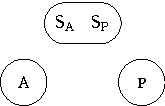
\includegraphics[width=0.3\linewidth]{figures/noun_alignment}
	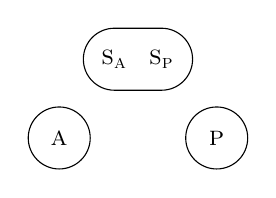
\begin{tikzpicture}
		\topleftnode[sa]{\gl{S\textsubscript{A}}}
		\toprightnode[sp]{\gl{S\textsubscript{P}}}
		\leftnode[a]{\gl{a}}
		\rightnode[p]{\gl{p}}
		\draw (a) circle (11.2pt);
		\draw (p) circle (11.2pt);
		\draw \convexpath{11.2pt}{sa,sp};
	\end{tikzpicture}
	\caption{Alignment of noun phrase flagging}
	\label{fig:alignment3}
\end{figure}

Noun phrases can be formed by nouns, which were discussed in the previous \chapref{ChapterNouns}, but also by personal and demonstrative pronouns, which are described in \sectref{sec:Pronouns}. Apart from possessive constructions, discussed in the previous chapter (\sectref{sec:Poss}), nouns are chiefly modified by verbs and relative clauses. \sectref{sec:ModNoun} explores the morphemes within a noun phrase that modify the head, including adjective-like derivations (\sectref{sec:adj}). Noun phrases can be coordinated and form a new constituent. Vamale distinguishes at least three: the comitative \textit{ma}, the additive coordinator \textit{ka} \qu{also, on top of that}, and \textit{hai} \goodtilde \textit{a} \qu{or}. They are all described in \sectref{sec:CordNP}.

 \section{Case marking}
\label{sec:Casmark}
\is{Case}

Case in this grammar refers to the marking of syntactic roles by morphemes. Vamale, like most Oceanic languages \parencites[37]{lynch_oceanic_2002}[496]{ross_morphosyntactic_2004}, does not mark syntactic roles on nouns with affixes. There are, however, prepositions that ``flag" the subject (\textit{ka}) and optional, oblique arguments (\textit{(nya)ko}). The choice of the morphemes is influenced by semantic and pragmatic factors: transitive subject noun phrases must be preposed by \textit{ka} (further discussed in \sectref{ssec:ka}), whereas intransitive subject nouns may take \textit{ka} in focused contexts. Oblique markers distinguish beneficiary and goal arguments from more generically patientive ones (see \sectref{sec:oblique}), and are sensitive to the animacy of the argument.

\subsection{Agentive marker \textit{ka} }
\is{Case!Agentive}
\label{ssec:ka}

This \textit{ka} is a subject marker (\ref{ex:sbj marker}).\footnote{The Pije cognate to the agentive marker is \textit{lu}.} Its allomorph \textit{a} is conditioned by a final consonant on the preceding word. It is obligatory before nouns and pronouns that agree with the verb in an \textbf{A} function, probably because unmarked transitive subjects can occur at the very end of long VOS sentences, and directly after an object noun phrase: 

\ea V (VV\ldots) O \textit{ka} A. \z

\noindent A clitic \textit{ka} is optional for S\textsubscript{A/P}, probably in an extension of the first scenario. In principle, Vamale participant flagging is a tripartite flagging system, since it disambiguates A, which must take \textit{ka}, from S, which may take \textit{ka}, from O, which may not take \textit{ka} (see \Cref{fig:alignment3}). %In nominalizations, this changes: while \textit{ka} is obligatory for A, and optional for both S and O (provided A is not explicit) (\ref{ex:nmlz ka}). 

\ea
\label{ex:sbj marker}
%	% \langinfo{}{}{} 
\gll 	{\ob}e=xaleke i={\ob}jili i=bwaakala{\cb\cb} ka yo	\\
	{[}1\gl{sg}=see \gl{def}.\gl{sg}=[build\_with\_wood \gl{def}.\gl{sg}=canoe]] \gl{sbj} 1\gl{sg}	\\
\glt  \qu{I see the building of the canoe.}		
\z

%\ea\label{ex:nmlz ka}
%
%%\langinfo{}{}{} The Oué family
%\gll	i hun-xale-a ka yo	
%	\gl{def}.\gl{sg}=\gl{nmlz}-see-3\gl{obj} \gl{sbj} 1\gl{sg}
%\glt	\qu{My way of seeing him (lit. the way of see him by me)}

%\a
%
%%\langinfo{}{}{} The following can be grammatical, if the unmarked A \textit{yo} is pronounced as a different clause or as an adjunct (pause, lower intonation of \textit{yo}). \textit{yo} must be flagged with \textit{ka} if it is to be part of the same clause as the verb. 
%\gll 	*{[}e=xaleke i [jili i bwaakala]] yo	
%	1\gl{sg}=see \gl{def}.\gl{sg}=build\_with\_wood \gl{def}.\gl{sg}=canoe \gl{sbj} 1\gl{sg}	
%\glt  (for: \qu{I see the building of the canoe})	
%

%\a
%
%\langinfo{}{}{} (\textit{e}- is a bound pronoun, \textit{yo} its free form)
%\gll e=xale-le ka yo	
% 1\gl{sg}-see-3\gl{pl} \gl{sbj} 1\gl{sg}	
%\glt \qu{I see them} (lit. \qu{i-see-them by I})	
%


Contrary to A arguments, which have to be marked with \textit{ka} unless fronted and thus not part of the clause anymore (e.g. \textit{yo, e=xale-a} \qu{me, I see them}, see \sectref{sec:fronting}), S arguments do not have to be marked with \textit{ka} (\ref{ex:optional_ka}).

\ea \label{ex:optional_ka}
\gll a=hup-wa (ka) i=jati\\
 3\gl{sg}=go.down-\gl{rep} (\gl{sbj}) \gl{def}.\gl{sg}=sea\\
\glt \qu{The tide goes down again.}
\z

\ea
\gll sinu (ka) mu=xho-ng\\
 suffer (\gl{sbj}) \gl{def}.\gl{du}=leg-1\gl{sg}.\gl{poss}\\
\glt \qu{My legs hurt.} (no index on \textit{sinu} because it is a stative verb)
\z


%``Mémoire en vue d'obtention de l'habilitation à diriger des recherches", Claire Moyse-Faurie, 2004
%
%can depend on TAM (Drehu), animacy (nemi), pronoun vs noun, transitivity.
%
%

%There is no copula (\textit{be}). Instead, Vamale juxtaposes a subject and a predicate (or a topic and a comment). The subject's only obligatory expression is the ``person marking index", a proclitic attached to the predicate. It can be omitted in imperative constructions and some other circumstances, such as same-subject coordinative clauses. The predicate includes TAM markers, which come between the preverbal subject marker and the predicate. 
%The fact that the subject NP can be left out and that the subject is a clitic (i.e phonologically and morphologically(?) part of the predicate) a problem for well-formedness conditions? xx

In nominalizations as well, \textit{ka} \qu{\gl{sbj}} obligatorily occurs to mark A (\ref{ex:nmlz-ka1}, \ref{a ka yo}). P may take a different \textit{ka} \qu{\gl{link}} when it is the only participant present in the construction (\ref{ex:nmlz-ka2}). If several participants co-occur, this option disappears, as the clause would otherwise become confusing. As this \textit{ka} only marks S and P, I gloss it subsequently as absolutive (see \sectref{kan}).


\ea\label{ex:nmlz-ka1}
\gll i=hun-saxhuti i=jaxhut nyanya-n-eong \textbf{ka} caacaa-n-eong	\\
 \gl{def}.\gl{sg}=\gl{nmlz}-narrate \gl{def}.\gl{sg}=story mother-\gl{poss}-1\gl{sg}.\gl{poss} \gl{sbj}  father-\gl{poss}-1\gl{sg}.\gl{poss}	\\
\glt \qu{my father's way of telling my mother's story}	
\z
%%todo check the ka glossing here

\ea\label{ex:nmlz-ka2}
\gll i=hun-vii (ka) i=jaxhut	\\
 \gl{def}.\gl{sg}=\gl{nmlz}-say \gl{link} \gl{def}.\gl{sg}=story	\\
\glt \qu{the way to say the story}	
\z

\ea\label{ex:nmlz-ka3}
\gll i=hun-moo (ka) i=mwa\\
 \gl{def}.\gl{sg}=\gl{nmlz}-be \gl{link} \gl{def}.\gl{sg}=house\\
\glt \qu{the nature of the house}
\z


\ea\label{a ka yo}
\gll	i=hun-xale-a ka yo	\\
	\gl{def}.\gl{sg}=\gl{nmlz}-see-3\gl{obj} \gl{sbj} 1\gl{sg}\\
\glt	\qu{my way of seeing him (lit. the way of seeing him by me)}
\z 


%\begin{comment}
%Stuff with -\textit{n} in \ref{ex:no n} has to with specificity. -n is generic, absence of -n means a specific (but not necessarily definite) NP \textit{i, eca, ca, li=X}.
%
%\ea
%\a
%
%\gll e=caihna i jaxhut	
% 1\gl{sg}=know \gl{def}.\gl{sg}=story	
%\glt \qu{I know the story}	
%
%
%\a
%
%\gll pathabu i yee	
% before \gl{def}.\gl{sg}=tree	
%\glt	\qu{in front of the tree}
%
%
%\z
%\end{comment}

The construction in (\ref{ex:coorka2}) is a more colloquial way of asking for the agent of an action and skips the usual pronoun \textit{kai} \qu{who?}. 

\ea \label{ex:coorka2}
\gll na a=nya ka?\\
 \gl{dem} 3\gl{sg}=put \gl{sbj}\\
\glt \qu{This, who put it there?} {[J8:35]}
\z 

\subsection{Oblique markers}
\label{sec:oblique}
%\todo{equally important are goals (and probably sources), most important are recipients!!!} 
%The markers discussed in \\sectref{sec:Casmark} mark semantic as well as syntactic roles.%, which suggests that there may not be cases as such.
%If there are no cases, there are no indirect arguments either, because this would imply two obligatory arguments marked differently. 

Vamale, like most canonic Oceanic languages \parencite[510]{ross_morphosyntactic_2004}, has no ditransitive verbs. Benefactive scenarios are expressed either with verb phrases or with the prepositions already mentioned in \sectref{sec:WCPP}. Four forms add a noun phrase to a verb phrase: \textit{nya} \qu{Beneficiary, Goal} (from the verb \qu{put, send, give}), \textit{si-} \qu{Recipient (human), Topic (human), Experiencer (animate), Goal (animate)} (from the noun \textit{si-} \qu{hand}), \textit{ko-} \qu{Ground, Theme, Stimulus} (from the preposition \qu{on}), and the combined forms \textit{nyasi-} and \textit{nyako-} \qu{give, for} discussed in more detail in \sectref{ssec:nyako}. In all cases, the added NP can be omitted, as in \textit{e (ila-ke) xaxhi/haxhi (nyakoo-n)} \qu{I (demand-\gl{tr}) forgiveness (for X)}. I thus argue that there are no indirect arguments in Vamale. Every NP introduced with \textit{nyako/nyasi}, \textit{ko} or \textit{nya} can be omitted without violating the verb's valency. This grammar will speak of oblique and (core) arguments. %\textit{ko} and \textit{nyasi} / \textit{nyako} are all oblique markers, with different semantic connotations.

\subsubsection{Benefactive \textit{nya}}
\is{Case!Beneficiary}
\label{ssec:benef_nya}

Most \textit{nya} forms are verbs and head a phrase themselves (\ref{ex:nyaV}). However, \textit{nya} may also act as an oblique marker and introduce a noun phrase. Since no non-contiguous serial verb construction (s)VoVo is otherwise attested in the language, (\ref{ex:nyakai}) is analyzed as a verb phrase \textit{vwa ena} \qu{do this} and the animate beneficiary marker \textit{nya}, which introduces the pronoun \textit{kai} \qu{who}. \textit{Nya} is also used as a spatial preposition meaning \qu{towards} (\sectref{ssec:prox_Adv}).
	
	\ea \label{ex:nyaV}
	\gll nya-a-me!\\
	 send-move.same.level-\gl{dir.cp}\\
	\glt \qu{Give it to me!}
	\z
	
	
	\ea
	\gll a=nya li=sale=ka-n (nya)si li=apuli	\\
	 3\gl{sg}=put \gl{def}.\gl{pl}=possession=\gl{poss}-3\gl{sg}.\gl{poss} \gl{ben} \gl{def}.\gl{pl}=person\\
	\glt \qu{He gives his goods to the people.}
	\z 
	
	\ea \label{ex:nyakai}
	\gll go=vwa ena nya kai?\\
	 2\gl{sg}=do \gl{dem}.\gl{dist} give who\\
	\glt \qu{For whom do you do that?}
	\z

\subsubsection{Oblique markers \textit{nyako-}, \textit{nyasi-}}
\label{ssec:nyako}
\is{Case!Oblique}
The prepositions \textit{nya-si} \qu{Recipient (human), Topic (human), Experiencer (animate)}, \textit{nya-ko} \qu{Recipient, Topic, Experiencer} are composed of the other three oblique markers \textit{nya} \qu{put, \gl{ben}}, \textit{ko-} \qu{on, \gl{obl}} and \textit{si-} \qu{hand, \gl{ben}}. 
They are derived from inalienable nominal forms (but do not take articles) and, similarly to locative nouns (see \sectref{ssec:WCPrepoNouns}), can have generic (\textit{-n}) or specific possessive markers (e.g. \textit{-ng} \qu{1\gl{sg}}, \textit{-m} \qu{2\gl{sg}}).
 
There are two main differences between \textit{nyasi} and \textit{nyako}. \textit{Nyasi} is restricted to animate participants, even human ones for some meanings, and suggests a less direct involvement of the marked NP: questions, demands (\ref{ex:nyasi_demand}) and gifts (\ref{ex:nyasi_gift}) are the main contexts in which it appears. The main difference between \textit{si} and \textit{nyasi} seems to be that \textit{si} marks the beneficiary of an already benefactive action (\ref{ex:si_nyasi2}), whereas \textit{nyasi} can add a beneficiary argument to any verb, see (\ref{ex:si_nyasi2b}).


\ea\label{ex:nyasi_demand}
\gll e=ila-ke nyasi-m i=vai\\
 1\gl{sg}=make.request-\gl{tr} \gl{ben}-2\gl{sg}.\gl{poss} \gl{def}.\gl{sg}=stone\\
\glt \qu{I (politely) ask you for the stone (lit. I request the stone from you).} {[B2:100]}
\z


\ea\label{ex:nyasi_gift}
\gll a=nya li=saleka-n si li=apuli\\
 3\gl{sg}=give \gl{def}.\gl{pl}=property-3\gl{sg}.\gl{poss} \gl{ben} \gl{def}.\gl{pl}=person\\
\glt \qu{He gives his things away to the people.} {[J7:14]}
\z


\ea
\label{ex:si_nyasi2}
\gll go ha-me saaguu-be see-me si-je mwa ca thôa koo-n\\
 \gl{cnj} go-\gl{dir.cp} support-1\gl{pl}.\gl{excl} same-all \gl{ben}-1\gl{pl}.\gl{incl} \gl{deict} in work \gl{obl}-\gl{ana}\\
\glt \qu{Now, come join to help us (\gl{excl}) to the benefit of us all (\gl{incl}) in this customary labour.} {[Bw:35]}
\z

\ea\label{ex:si_nyasi2b}
\gll ta-xhavwaleke ma gase=bo vwa nyasi-le\\
 sitting-wait \gl{subr} 1\gl{pl}.\gl{incl}=\gl{irr} do \gl{ben}-3\gl{pl}\\
\glt \qu{(They) sit around waiting for us to do it for them.} {[GB:17]}
\z

Similar in functions, \textit{nyako} is generally more common, as it marks human and non-human participants alike. Similarly to \textit{ko}, \textit{nyako} can introduce a Stimulus (\ref{ex:nyako_mwani}). \textit{Nyasi} is also only attested once for the function of topic marker, and was in a fronted position: \textit{nyasi Leenhardt, cip=e xa-xale-a} \qu{concerning Leenhardt, I never saw him} (\ref{ex:nyasi}). \textit{Nyako} is an unmarked particle to introduce a topic (\ref{ex:nyako1}).


\ea\label{ex:nyasi1}
\gll tha lu=mata nyasi i=jamwa-n sohmu-n\\
 \gl{ass}=3\gl{du} sing for \gl{def}.\gl{sg}=father-\gl{poss} study-\gl{nspec}\\
\glt \qu{They sing for the teacher.}
\z


\ea\label{ex:nyako1}
\gll tha lu=mata nyako i=jamwa-n sohmu-n\\
 \gl{ass}=3\gl{du} sing \gl{obl} \gl{def}.\gl{sg}=father-\gl{poss} study-\gl{nspec}\\
\glt \qu{They sing about/to the teacher.}
\z

\ea\label{ex:nyako_mwani}
%\langinfo{}{}{}  
\gll e=vwa xaleke nyako li=mwani-n-eong\\
 1\gl{sg}=do buy for \gl{def}.\gl{pl}=money-\gl{poss}-1\gl{sg}.\gl{poss}\\
\glt \qu{I do (buy) according to my means.} {[vamale-181107-jpnelemwa-06\_LR 0:12:24-0:12:26]}
\z

 
\subsubsection{Oblique marker \textit{ko-}}
\is{Case!Oblique}
\label{ssec:koon}

The preposition \textit{ko-} introduces mainly instruments to the verb phrase (see (\ref{ex:ko_beer}) and (\ref{ex:ko_knife})), as well as other oblique noun phrases: Stimulus (\ref{ex:ko_stim}, \ref{ex:ko_oblique}), Themes (\ref{ex:ko_about}) and Ground (e.g. \textit{bitake ko-n koltaa} \qu{turn around on the street}\footnote{\textit{bitake} \qu{rotate on a flat Ground} takes a \textit{ko}-marked oblique noun phrase when the Ground is specified.}). They are called oblique here, because the verb phrase remains grammatical without the noun phrase introduced by \textit{ko}. A nominal modifier construction with \textit{ko-} is described in \sectref{ssec:ko_N}.


\ea\label{ex:ko_beer}
\gll e=kon udu ko-n bia\\
 1\gl{sg}=\gl{prog} drink.cold \gl{obl}-\gl{nspec} beer\\
\glt \qu{I am getting drunk with beer.} {[2019-07-25 JP grammaire:16]}
\z


\ea\label{ex:ko_knife}
\gll a=vi nyakoo-be nyima-n ma yaai ko-n thala\\
 3\gl{sg}=say \gl{obl}-1\gl{pl}.\gl{excl} will-3\gl{sg}.\gl{poss} \gl{subr} saw \gl{obl}-\gl{nspec} knife\\
\glt \qu{He told us that he wants to cut it by knife.} {[GP:78]}
\z

\ea \label{ex:ko_stim}
\gll e-sinu-o koo-n\\
 \gl{mid}-suffer-1\gl{sg} \gl{obl}-\gl{ana}\\
\glt \qu{I suffer from it.} {[G5:51]}
 \z
 
\ea
\gll yo hmwet-eo ko i=vaya-ca\\
 1\gl{sg} tired-1\gl{sg} \gl{obl} \gl{def}.\gl{sg}=work-\gl{prox}\\
\glt \qu{I am fed up with/tired of this work.} (in local French: \textit{je suis fatigué de ce travail}) {[X9:25]}
\z


\ea\label{ex:ko_oblique}
\gll Abe=holeke nya-koo-m au Nyaanya ko li=vaaya a= go=vwa cahni Bako\\
 1\gl{pl}.\gl{excl}=thank.for put-on-2\gl{sg} oh Mummy \gl{obl} \gl{spec}.\gl{pl}=work \gl{rel}= 2\gl{sg}=do here Bako\\
\glt \qu{We thank you, oh Mommy, for the works you did here in Bako.} {[2017-07-21 Chant de deuil:8-9]}
\z

\ea
\gll go=see ko i=da?\\
 2\gl{sg}=cry \gl{obl} \gl{def}.\gl{sg}=what\\
\glt \qu{Why do you cry?}
\z 

While there are adjuncts introduced by \textit{ko}, notably causes (\ref{ex:ko_hmwaeke}) and locations (\ref{ex:ko_on}), the ones I call oblique are semantically specified by the verb. For some verbs, noun phrases introduced by \textit{ko} have become core arguments and are not omissible without changing the meaning (e.g. \textit{(vwa) icu} \qu{barter (intransitive)}, \textit{icu-ko-} \qu{sell} in (\ref{ex:ko_on})). This scenario is discussed in more detail in \sectref{ssec:V_ko}. 
This inalienable \textit{ko-} is not to be confused with the conjunctions \textit{ko} \qu{but} and \textit{kon} \qu{and then} (\ref{ex:ko_on}), the progressive particle \textit{kon} (\ref{ex:ko_beer}), nor with the subordinator \textit{ko} \qu{because}, discussed in \sectref{sec:conj_ko}.


\ea\label{ex:ko_on}
\gll kon tha=abe=saavi cama=be icu-koo-n ko-n \textit{marché}\\
 \gl{cnj} \gl{ass}=1\gl{pl}.\gl{excl}=dig.up if=1\gl{pl}.\gl{excl} barter-\gl{obl}-\gl{ana} on-\gl{nspec} market\\
\glt \qu{And then we dig them up whenever we sell them at the market.} {[AG1:22]}
\z

\ea\label{ex:ko_about}
\gll ko na kai a=eca-kau ko niena-aen\\
 but \gl{dem} who \gl{rel}.3\gl{sg}=learn-2\gl{du} \gl{obl} \gl{dem}.\gl{pl}-\gl{dist}\\
\glt \qu{But who taught you all this? (lit. but this who that teach you about this)} {[GC:81]}
\z


\section{Pronouns}
\label{sec:Pronouns}
\is{Pronouns}
There are three types of openly expressed arguments. The free form, called ``pronoun" here, can be fronted, take the agentive marker \textit{ka} and the beneficiary \textit{nya}, is used to call people, for topicalization, and often occurs in imperatives. This group includes personal pronouns (\sectref{ssec:persPN}, listed in \Cref{tab:freePN2}), demonstrative pronouns (\sectref{ssec:Prox}), and stand-in question words \textit{kai} \qu{who} and \textit{da} \qu{what} (\ref{ex:da}). The latter can take a singular article in marked scenarios, see (\ref{ex:ida}).

\begin{table}
	\centering
	\caption{Free pronouns}
	\begin{tabular}{l llll}
	\lsptoprule
		& 1 (\gl{excl})&	1+ (\gl{incl})&	2&	3\\\midrule
		\gl{sg}&	\textit{yo}&&		\textit{go}&	\textit{ya}\\
		\gl{du}&	\textit{abu}&	\textit{gasu}&	\textit{gau}&	\textit{lu}\\
		\gl{pl}&	\textit{abe}&	\textit{gaa}&	\textit{gavwe}&	\textit{le}\\
	\lspbottomrule
	\end{tabular}
	\label{tab:freePN2}
\end{table}


\ea\label{ex:da}
\gll ko go=vii da?\\
 \gl{cnj} 2\gl{sg}=say what\\
\glt \qu{But what are you saying?} {[X1:1]}
\z

\ea\label{ex:ida}
\gll gaa tha gase=juu tena go tha gase=thii mae ka a=bo xahnang i=da?\\
 1\gl{pl}.\gl{incl} \gl{ass} 1\gl{pl}.\gl{incl}=real listen then \gl{ass} 1\gl{pl}.\gl{incl}=light fire \gl{cnj} 3\gl{sg}=\gl{irr} good \gl{def}.\gl{sg}=what\\
\glt \qu{We'd listen well, and we'd light fires [anyway] and what's supposed to be good then?} {[RP:14]}
\z

The other forms are bound (\Cref{tab:markers4}). \gl{S\textsubscript{A}} participants are indexed on the predicate by proclitic particles called \qu*{bound pronouns}. \gl{S\textsubscript{P}} participants are indexed on stative verbs via suffixes, as are undergoers. They will be further treated in \chapref{ChapterVerbs}.

\begin{table}
	\centering
	\caption{Subject and object markers for active and stative verbs}
	\begin{tabular}{lllll}
	\lsptoprule
		&	Free form	& \gl{a}=/\gl{S\textsubscript{A}}= & -\gl{S\textsubscript{P}} & -\gl{p}\\\midrule
		1\gl{sg} & \textit{io} & \textit{e} & \textit{-o(ng)} & \textit{-o} \\
		1\gl{du}.\gl{incl}& \textit{gasu} & \textit{gasu} & \textit{-gasu} & \textit{-kaeu}\\
		1\gl{pl}.\gl{incl} & \textit{gaa/gase} &\textit{ga(se)}&\textit{gaa}&\textit{-kaa}\\
		1\gl{du}.\gl{excl} & \textit{abu} & \textit{abu} & \textit{-abu} & \textit{-(a)bu}\\
		1\gl{pl}.\gl{excl} & \textit{abe}& \textit{abe} & \textit{-abe} & \textit{-(a)be}\\
		2\gl{sg} & \textit{go} &\textit{go} & \textit{-go} & \textit{-ko}\\
		2\gl{du} & \textit{gau} & \textit{gau} & \textit{-gau} & \textit{-kau}\\
		2\gl{pl} &\textit{gavwe}& \textit{gavwe} & \textit{-gavwe} & \textit{-kavwe}\\
		3\gl{sg} & \textit{ia} & \textit{a} & \textit{-(e)a} & \textit{-(e)a}\\
		3\gl{du} & \textit{lu} &\textit{lu} & \textit{-lu} & \textit{-lu}\\
		3\gl{pl} & \textit{le} & \textit{le} & \textit{-le} & \textit{-le}\\
	\lspbottomrule
	\end{tabular}
	\label{tab:markers4}
\end{table}

There is a difference in marking between \gl{S\textsubscript{P}}, \gl{S\textsubscript{A}}/\gl{a}, and \gl{p}, leading to a tripartite split S alignment in the marking of participants on the predicate. The undergoer markers are also bound pronouns, because they are in complementary distribution with undergoer NPs, meaning that either the object of the verb is expressed openly (\ref{ex:xaleke_i}), in which case the verb may bear a transitivity marker, or the object is expressed by the suffix (\ref{ex:xalea}), in which case no open object NP may follow (\ref{ex:xalea2}).

	
	\ea\label{ex:xaleke_i}
	\gll a=xaleke i=pupwaale\\
	 3\gl{sg}=see \gl{def}=European\\
	\glt \qu{He sees the European.}
	\z
	
	\ea\label{ex:xalea}
	\gll a=xale-a\\
	 3\gl{sg}=see-3\gl{sg}\\
	\glt \qu{He sees him.}
	\z
	
	\ea\label{ex:xalea2}
	\gll *a=xale-a i=pupwaale\\
	  3\gl{sg}=see-3\gl{sg} \gl{def}=European\\
	\glt (\qu{He sees the European.})
	\z
	
Following Kroeger, a syntactic function is unique to one argument \parencite[20]{kroeger_analyzing_2004}. Since free pronouns are noun phrases, they cannot coexist with the noun with which they would share a referent in the same clause. %Hence the object marker paradigm is a pronominal one.%that last sentence doesnt make sense

\subsection{Personal pronouns}
\label{ssec:persPN}

The \qu*{subject markers}, as they are called in the literature on New Caledonian languages, are obligatory and not in complementary distribution with open noun phrases possessing the same referent. This may be due to the basic word order VOS, where the object follows the verb immediately, but the subject may need a \qu*{reminder} at the beginning.
This means that they are not pronouns in the traditional sense. They occur before aspect markers, and are proclitics which attach to predicates. They are listed in \Cref{tab:markers4}. 

Dual personal pronouns, as well as dual articles, are used for polite speech: while \textit{gau} 2\gl{du} is used to politely address a single person, thus augmenting their importance, \textit{muca} \gl{indf}.\gl{du} is used in offering things, to diminish the size of the offer, as in (\ref{ex:muca}).

\ea \label{ex:muca}
\gll fe muca=nyu!\\
 take \gl{indf}.\gl{du}=fish\\
\glt \qu{Take some fish! (more than two)}
\z
Dual pronouns, and plural pronouns, are used differently than in European languages when including someone with the addressee, i.e. \qu{with whom did you go?} or \qu{you and your uncle's village} (\ref{ex:bwanpu}).

\ea  \label{ex:bwanpu}
\gll i=bwanpu-n-abu ma vwoon-ong\\
 \gl{def}.\gl{sg}=country-\gl{poss}-1\gl{du}.\gl{excl} \gl{com} uncle-1\gl{sg}.\gl{poss}\\
\glt \qu{my and my maternal uncle's village} {[vamale-181107-jp\_nelemwa-06: 00:12:56-00:12:58]} 
\z

\subsection{Demonstrative pronouns}
\label{ssec:Prox}
\is{Pronouns!Demonstrative pronouns}

Demonstrative pronouns in Vamale distinguish number: those prefixed with \textit{e-} are the singular forms,\footnote{Possibly derived from the singular article \textit{i}. Both \textit{vi} \qu{\gl{def}.\gl{sg}} and \textit{ve-hni} \qu{\gl{dem}.\gl{prox}} are attested in older speakers.} those with \textit{ni-} the plural, and with \textit{mu-} the dual forms. The dual forms are rare. The forms are listed in \Cref{tab:dem_pro}. Note that the plural forms feature two transparent morphemes: the plural \textit{ni-} and the proximal\slash distal suffixes \textit{-hni} and \textit{-na} which are also found in the verb \textit{hmwa-ehni} \qu{be.like-this} and \textit{hmwa-ena} \qu{be.like-that}. The third part of the plural pronouns is a non-transparent \textit{-e-}. This may be a former singular prefix, as is still featured by the singular forms, onto which a plural morpheme would have been prefixed without replacing it, possibly meaning that \textit{niehni} was formed much later. On the other hand, \textit{ehni} is still pronounced \textit{vehni} by elders, and the singular article is still \textit{vi} in comparatively archaic Vamale Usa, but \textit{nivehni} is not attested anywhere. A simple epenthetic function seems unlikely given that the dual forms lack it.

\begin{table}
		\caption{Demonstrative pronouns}
		\begin{tabular}{lll}
		\lsptoprule
			& proximal & distal\\\midrule
			\gl{sg} & \textit{e-hni} & \textit{e-na}\\
			\gl{du} & \textit{muu-hni} & \textit{muu-na}\\
			\gl{pl} & \textit{ni-e-hni} & \textit{ni-e-na}	\\
		\lspbottomrule
		\end{tabular} 
	\label{tab:dem_pro}
\end{table}


The suffix \textit{-hni} has the stative verb cognate \textit{hni-} \qu{proximal} %and  
in Bwatoo \parencite[43]{rivierre_bwatoo_2006}. Rivierre calls demonstratives verbs \parencite[42]{rivierre_bwatoo_2006}, which makes sense given that they can take stative subject suffixes: \textit{ehni-o} \qu{here I am}. Its distal counterpart \textit{-na} does not seem cognate to Bwatoo \textit{hanaa-} \qu{be here}, but could be cognate to \textit{nai-} \qu{recently mentioned} \parencite[43]{rivierre_bwatoo_2006}.
The latter verb \textit{nai-} \qu{recently mentioned} is a possible hint at the real function of \textit{-hni} and \textit{-na}: the suffixes being able to distinguish between recently mentioned information and some that was mentioned longer ago, or not at all (but is general knowledge).\footnote{Bwatoo furthermore has the stative verb \textit{hutaa-} \qu{below} %and \textit{nai-} \qu{recently mentioned}
 which does not find an exact counterpart in Vamale (see example \ref{ex:nai}) \parencite[43]{rivierre_bwatoo_2006}.}


	\ea 
\label{ex:nai}
	(Bwatoo)\\
	\gll go vwa ni ma-nai-a\\
	 2\gl{sg} do \gl{def}.\gl{pl} \gl{nmlz}-recently.mentioned-3\gl{sg}\\
	\glt \qu{Do these things!} \parencite[43]{rivierre_bwatoo_2006}
	\z	
	
	\ea
	(Vamale)\\
	\gll go=vwa li=aman-ca\\	
	 2\gl{sg}=do \gl{def}.\gl{pl}=thing-\gl{prox}\\
	\glt \qu{Do the things there.}
	\z


The pronouns are mostly used as topics or comments in equative constructions (\ref{ex:ehni}), though \textit{ena} is also used to express agreement, like in English \qu{exactly}. The latter use is also attested with \textit{hmwaana} \qu{be like that}. \textit{Hmwaani} \qu{be like this} cannot be used to comment on a previous utterance. \textit{-Na} and \textit{-hni} may thus be more of an engagement-distinguishing pair than really about distance, i.e. mark whether something is close to the speakers' attention. The demonstrative suffixes \textit{-ca} and \textit{-aen} can take a similar function.

\ea \label{ex:ehni}
\gll  tha pa i=hun-moo-o ve-hni\\
 \gl{ass} \gl{prf} \gl{def}.\gl{sg}=\gl{nmlz}-be-1\gl{sg} \gl{dem}-\gl{prox}\\
\glt \qu{This is my (elder's) way.} (\textit{pa} conveys that his life has come to this) {[HC19:61]}
\z

\textit{niena} \qu{\gl{dist}.\gl{pl}} is the only form attested as \textit{nienaen} with an additional \textit{-aen} \qu{dist} suffix, which usually only applies to nouns, and has the idiosyncratic meaning \qu{all that}, see (\ref{ex:nienaen}). There is no equivalent \textit{niena-ca} form using the nominal proximal suffix, which is reminiscent of the \textit{ena}\slash\textit{hmwaana} cases only using the more distal form for abstract functions.


\ea \label{ex:nienaen}
\gll cahma niehni abe cabeen xhaohmu-n-go ja cip-abe yajooke mwa nien-aen\\
 \gl{top} \gl{dist}.\gl{pl} 1\gl{pl}.\gl{excl} \gl{indf}.\gl{pl} elder-\gl{poss}-2\gl{sg} \gl{prf} \gl{neg}-1\gl{pl}.\gl{excl} attain now \gl{dist}.\gl{pl}-\gl{dist}\\
\glt \qu{When it comes to these (works of our ancestors), we elders of yours already don't attain all of that anymore.} {[CP1:49]}
\z



\label{ssec:mehni}

The prefix \textit{me} \qu{all} is attested as a prefix to the demonstrative pronoun \textit{ehni} (\ref{ex:mehni}), but no other nominal element. The related pre-verb \textit{me} is discussed in \sectref{ssec:mee}.

\ea \label{ex:mehni}
\gll nyeet ca-n fava-vwasiteke na ca i=thuatit a= le=fe-kaa ka me-ehni cahni pala-je\\
 when in-\gl{nspec} four-pray \gl{dem} in \gl{def}.\gl{sg}=day \gl{rel}= 3\gl{pl}=take-1\gl{pl}.\gl{incl}.\gl{obj} \gl{sbj} all-\gl{dem}.\gl{prox} here home-1\gl{pl}.\gl{incl}.\gl{poss}\\
\glt \qu{When, on Thursday, it was on that day that those all came to fetch us here in our home.} {[GP:2-3]}
\z 

\is{Demonstratives!Topical demonstrative \textit{na}}
Related to \textit{ena}, there is another, very common, form, \textit{na}, which can only be used as the topic of a clause. Whether that clause is an equative construction involving only nominal phrases (including the demonstrative pronouns \textit{ena} and \textit{ehni}), or one with a verbal predicate, \textit{na} comes first. The pronoun cannot be used for subjects in the traditional VOS word order, nor take flagging. 

\ea
%\langinfo{}{}{}  
\gll  ‎‎\textit{tu} \textit{vois}, na tha cipa ca=aman a= le=thêên thêên ca-n magasî. na le=vwa-suki lait.\\
 you see \gl{dem} \gl{ass} \gl{neg} \gl{indf}.\gl{sg}=thing \gl{rel}= 3\gl{pl}=run run in-\gl{nspec} shop \gl{dem} 3\gl{pl}=do-price rice\\
\glt \qu{You see, it's not something they'd run run to the shop [for], they'd pay for rice...} {[KP:82]}
\z

The demonstrative \textit{na} has a form used only in insistent scenarios, often associated with repetition: \textit{ha}.

\ea
\gll xa-vuki vai ko-n thexhwaade ha li=kalen\\
 \gl{agt}.\gl{nmlz}-stem rock at-\gl{nspec} T. \gl{dem} \gl{def}.\gl{pl}=k.\\
\glt \qu{The guardians of the Thexhwaade rock are the Kalens.} {[DP:12]}
\z

\section{Fronting}
\label{sec:fronting}
\is{Fronting}

The subject is often fronted, but may then still occur after the verb, indicating that a fronted subject is not a constituent of the clause.\footnote{Prosodically, too, the fronted subject has an own contour, which yields two intonation units: the fronted subject, and the clause.} Fronting can be used to focus on any constituent, a resumptive morpheme remaining in the matrix clause.
The topic markers \textit{cahma} and \textit{nyasi} may precede the fronted constituent (\ref{ex:cahma}, \ref{ex:nyasi}).

\is{Fronting!Topic marker \textit{cahma}}
With most speakers, the particle is pronounced [tɕamã], but since two older speakers, Mrs.\ Madeleine Bonu Fouan and Mr.\ Philippe Dego Gohoupe (e.g. in (\ref{ex:cahma})), pronounce it with an audibly voiceless nasal [tɕaʰm̥a], I distinguish this word from \textit{cama} \qu{if, when.\gl{irr}}, which introduces subordinate and insubordinate clauses, but never a fronted noun phrase.


\ea\label{ex:cahma}
\gll ka cahma yo, tha gavwe=paa hmaa-ko-ong naen gavwe bwa hmaa-ko-ong ka pala\\
 \gl{cnj} \gl{top} 1\gl{sg} \gl{ass} 2\gl{pl}=\gl{prf} arrive-on-1\gl{sg} now 2\gl{pl} \gl{ipfv} arrive-on-1\gl{sg} \gl{cnj} talk\\
\glt \qu{But me, you have found me now, you found me and [we] spoke.} {[HC19:59]}
\z

\ea
\gll ca i=wadan-aen, \textbf{cahma} Xa-xhwi Apuli, {\ob}...{\cb} a=kon e-hnyimake ma a=xhwii-le \textbf{hai} \textbf{ma} a=cee-le ma le=han.\\
 in \gl{def}.\gl{sg}=time-\gl{dem} \gl{top} \gl{agt}.\gl{nmlz}-eat person {} 3\gl{sg}=\gl{prog} \gl{refl}-think \gl{subr} 3\gl{sg}=eat-3\gl{pl} \gl{cnj} \gl{subr} 3\gl{sg}=leave-3\gl{pl} \gl{subr} 3\gl{pl}=go\\
\glt \qu{At this moment, Maneater wondered whether he was going to eat them or let them go.} {[GC:107]}
\z


\ea\label{ex:nyasi}
\gll nyasi Leenhardt, cip=e xa-xale-a\\
 \gl{top} L. \gl{neg}=1\gl{sg} \gl{agt}.\gl{nmlz}-see-3\gl{sg}.\gl{obj}\\
\glt \qu{Concerning Leenhardt, I never saw him.} {[HC1:36]}
\z

  \section{Modifying a noun}
  \label{sec:ModNoun}
Noun phrases feature various words that modify their head: particles can be preposed to the noun, see \textit{se} and \textit{been} \qu{other} (\sectref{sec:ise}), as well as the quantifying particles discussed in \sectref{ssec:Quant}. Two forms, \textit{vataan} \qu{each} and \textit{me} \qu{all} are used (see \sectref{ssec:Preverbs}), but also attested in noun phrases (\textit{me} is restricted to pronouns) (\ref{ex:vatan2}). A small sub-class of verbs is described in \sectref{ssec:Verbs_n} that integrate the noun phrase. Nouns can be modified by other nouns and by relative clauses (\sectref{sec:RelCl}), whose subordinating particle is introduced in \sectref{sec:a}. The prepositional noun \textit{ko-} \qu{on} (\sectref{ssec:ko_N}) coordinates nouns into a possessive-like construction. %While this subordination, essentially a relative clause construction, used to be marked only for animated nouns, this distinction is now disappearing.
Possessors are discussed in the chapter on nouns (\sectref{sec:Poss}). Finally, demonstrative suffixes, while not words, dock onto nouns and pronouns alike, and add information about the saliency or proximity of the word (\sectref{ssec:DemSuff}).

\ea \label{ex:vatan2}
\gll tha lu=tena nyasi li=vatan xhaohmu\\
 \gl{ass} 3\gl{du}=\gl{obl} \gl{def}.\gl{pl}=each elder\\
\glt \qu{They heard about the different/various ancestors.} {[GT:6]}
\z

\subsection{Particles \textit{se}, \textit{been} \qu{other}}
\label{sec:ise} \is{Particle!\textit{se} \qu{other}} \is{Particle!\textit{been} \qu{other}}

Vamale features two function words that can both occur between the article and the noun, and act as a placeholder for the noun after the article. One is \textit{se} \qu{other} (\ref{ex:i se apuli}). It is derived from the stative verb \textit{se-} \qu{one, be one/the same} which can be used predicatively as well as attributively (\ref{ex:i se apuli2}). \textit{Se-} is also a preverb (see \sectref{ssec:se-me}). \textit{Se} is attested in two cases preceding definite noun phrases without \textit{i} or \textit{li}/\textit{ni} (\ref{ex:see1}, \ref{ex:see2}), but this use was not further investigated and must be left to future research. The other function word is \textit{been}, derived from the noun \textit{bee-n} \qu{peer-3\gl{sg}.\gl{poss}} (\ref{ex:li been apuli}). Like \textit{se}, it is not inflected. Both \textit{se} and \textit{been} are attested with indefinite articles as well (\ref{ex:case}). We thus find \textit{i/eca se} \qu{the\slash some other}, \textit{li}\slash\textit{mu}\slash\textit{muca}\slash\textit{ca been} \qu{the\slash some others}. Both \textit{been} and \textit{se} have a different meaning than the nominal and verbal forms, and can be used as placeholders for the modified noun (\ref{ex:case}, \ref{ex:cabeen}). The co-occurrence of the particles with nouns (\ref{ex:i se apuli}) excludes an analysis as pronouns. 


\ea\label{ex:i se apuli}
\gll i=se apuli\\
 \gl{def}.\gl{sg}=one person\\
\glt \qu{the other person}
\z


\ea\label{ex:i se apuli2}
\gll i=apuli a= se-a\\
 \gl{def}.\gl{sg}=person \gl{rel}= one-3\gl{sg}\\
\glt \qu{the person who is alone}
\z


\ea\label{ex:li been apuli}
\gll li=bee-n apuli\\
 \gl{def}.\gl{pl}=peer-\gl{poss}.\gl{nspec} person\\
\glt \qu{the other people}
\z


\ea\label{ex:see1}
\gll lu=moo ca se mwa-n-lu\\
 3\gl{du}=stay in one house-\gl{poss}-3\gl{du}.\gl{poss}\\
\glt \qu{They stay in the same house. (lit. they stay in one house of theirs)} {[J5:58]}
\z


\ea\label{ex:see2}
\gll i=that cipa xa-sivu ca la a= se la\\
 \gl{def}.\gl{sg}=wind \gl{neg} \gl{agt}.\gl{nmlz}-blow in location \gl{rel}= one location\\
\glt \qu{The wind does not always blow in the same place.} (lit. \qu{the wind is not a constant blower in a place that is one/the same place}) {[J4:14]}
\z 


\ea\label{ex:case}
(Note that \textit{ecase} \qu{someone} is a pronoun (see \sectref{ssec:eca}))\\
\gll na cip=e tena ca a= vi ka ca see\\
 \gl{dem} \gl{neg}=1\gl{sg} hear \gl{sg}.\gl{indf} \gl{rel}= say \gl{sbj} \gl{sg}.\gl{indf} one\\
\glt \qu{I haven't heard anything said by anyone.} {[KL:171]}
\z

\ea
\label{ex:cabeen}
\gll Tha faphâke nyako wîî ca been  \\
 \gl{ass} believe \gl{obl} strength \gl{pl}.\gl{indf} other\\
\glt \qu{We hope for the strength of others.} {[KL:171]}
\z

\subsection{Quantification}
\label{ssec:Quant}
\label{ssec:meeka-n}
\begin{sloppypar}
Nouns are mostly quantified with verbs. Numbers are expressed through verbs, as are forms like \textit{hmai-n} \qu{many} in (\ref{ex:hmain}) and the derived middle form \mbox{\textit{e-hmai-n}} \qu{more and more (countable)} (see \sectref{ssec:MID_unbounded}). Non-verbal quantifiers include \textit{jaa} \qu{much}, \textit{mu} \qu{few (uncountable)} as well as \textit{meeka-n}, all signifying uncountable and thus generic masses: \textit{jaa apuli} \qu{too many people}, \textit{mu mwani} \qu{little money}, \textit{meeka li=apuli} \qu{all the people}. 
\end{sloppypar}

\ea \label{ex:hmain}
\gll go cahma naen mwa xada hê ja mu e-xhopwe mwa i=hun-moo-gaa \textbf{hmain-ga} mwa \\
 \gl{cnj} \gl{top} now \gl{rep} differently yes \gl{prf} \gl{iter} \gl{mid}-grow \gl{rep} \gl{def}.\gl{sg}=\gl{nmlz}-stay-1\gl{pl}.\gl{incl} many-1\gl{pl}.\gl{incl} \gl{rep}\\
\glt \qu{But today it's nevertheless... yeah, it's ended up growing more and more, our way of life, we're numerous now.} {[KP:77]}
\z

One form has been attested so far with a quantifying meaning, but able to take alienable possessive morphology: \textit{meeka-n} \qu{all}. \textit{Meeka-n} cannot take articles, and precedes the noun phrase (\ref{ex:meekan}). 

 \ea \label{ex:meekan}
\gll le=kiica ka meeka li=been thamo, ma ca-n e-dawee-le i=a= yata-n In Thu.\\
 3\gl{pl}=jealous \gl{sbj} all \gl{def}.\gl{pl}=other woman while in-\gl{nspec} \gl{mid}-between-3\gl{pl} \gl{def}.\gl{sg}=\gl{rel}= name-3\gl{sg}.\gl{poss} Skin Banyan\\
\glt \qu{All the women were jealous, but among them was the one whose name was Banyan Bark.} {[GC:6]}
\z


\ea\label{ex:meekan2}
\gll cipa goon m=e saxhuti nyaako-m meeka i=jaxhut \\
 \gl{neg} enough \gl{subr}=1\gl{sg} tell to-2\gl{sg}.\gl{poss} all \gl{def}.\gl{sg}=story  \\
\glt \qu{I can't tell you the entire story (lit. everything of the story).} {[X9:31]}
\z

\textit{meeka-n} \qu{all} can be used after a noun as well, in which case it carries an anaphoric suffix \textit{-n} (\ref{ex:meekanafter}). 

\ea \label{ex:meekanafter}
\gll le=hame ka li=thamo meeka-n\\
 3\gl{pl}=go-\gl{dir.cp} \gl{sbj} \gl{def}.\gl{pl}=woman all-\gl{ana}\\
\glt \qu{All the women come.}  {[vamale-181127-jp\_nelemwa-1: 00:01:03-00:01:05]}
\z

\subsection{Relativizer \textit{a}}
\label{sec:a}
The relativizer \textit{a} subordinating the modifying clause (\ref{ex:a}) to the modified noun phrase is often omitted if the subordinated clause is short, same-subject, or stative (in the case of verbal predicates). Relative clauses are discussed in \sectref{sec:RelCl}.

\ea \label{ex:a}
\gll go=xaahni eca=paatelo a= xa-xahnang\\
 2\gl{sg}=see \gl{indf}.\gl{sg}=trousers \gl{rel}= \gl{agt}.\gl{nmlz}-good\\
\glt \qu{You see some nice pants.} {[KL:66]}
\z

\ea
\gll yo th=e=bwa xaleke li=xhaohmu a= le=mu vap ko-n da \\
 1\gl{sg} \gl{ass}=1\gl{sg}=\gl{ipfv} see \gl{def}.\gl{pl}=old \gl{rel}= 3\gl{pl}=\gl{freq} hunt \gl{obl}-\gl{nspec} spear \\
\glt \qu{Me, I still used to see the elders who'd hunt with a spear.} {[KL:162]}
\z

\subsection{Noun phrase subordinator \textit{ko-}}
\label{ssec:ko_N}

Especially for new concepts, a construction is used which is reminiscent of the French one N + \textit{de} + N, e.g. \textit{voiture\textsubscript{i} de service\textsubscript{ii}} \qu{work\textsubscript{ii} car\textsubscript{i}}. The modified noun comes first, with a noun phrase subordinated by the preposition \textit{ko-} following it: \textit{watuut ko-n vaya} \qu{work car} (lit. \qu{car on-\gl{nspec} work}). This prepositional noun \textit{ko-} \qu{on; \gl{obl}} described in \sectref{ssec:koon}, usually takes a generic noun phrase (\ref{ex:ko_generic}), but specific ones are also attested (\ref{ex:ko_specific}). The resulting construction looks like a possessive one, but is analyzed here as a prepositional phrase nested in a noun phrase.


\ea\label{ex:ko_generic}
\gll bwa \textit{sauver}-ong ka ehni a=vi, \textit{chambre-à-air} ko-n velo\\
 \gl{ipfv} save-1\gl{sg}.\gl{obj} \gl{sbj} \gl{dem} 3\gl{sg}=say air.chamber on-\gl{nspec} bike \\
\glt \qu{What he said saved me, ``bike air chambers" [to train my broken arm].} {[KG:175]}
\z

\ea\label{ex:ko_specific}
\gll bee-lu ko i=moo\\
 peer-3\gl{du} \gl{obl} \gl{def}.\gl{sg}=stay\\
\glt \qu{roommates} {[JN1:174]}
\z

\textit{ko} is derived from the prepositional noun meaning \qu{on}, and is a member of a polyvalent group of \textit{ko} forms, including an oblique marker (\sectref{ssec:koon}), subordinators (\sectref{sec:ko_cause} and \sectref{sec:conj_ko}), and, though it lexicalizes the non-specific marker \textit{-n}, the progressive marker \textit{ko(o)n} (\sectref{sec:kon}).



\subsection{Demonstrative suffixes}
\label{ssec:DemSuff}
Vamale features demonstrative pronouns, discussed in \sectref{ssec:Prox}. One of the latter, \textit{niena} \qu{\gl{dem}.\gl{pl}.\gl{dist}}, and common nouns, are the only words able to take demonstrative suffixes. The suffixes in question are \textit{-ca} \qu{\gl{prox}.(\gl{dir.cp})}, which can denote visible or otherwise salient entities, and \textit{-aen} \qu{\gl{dist}}, which marks more generally distant ones. A saliency or spatial distinction appears in Bwatoo only with the forms \textit{-hni} and \textit{-hanaa} \parencite[43]{rivierre_bwatoo_2006} discussed in \sectref{ssec:Prox}, but neither Bwatoo nor other West Coast dialects seem to feature \textit{-ca} and \textit{-aen}. Hienghène languages make the proximal/distal distinction as well, with a third degree (close but not to the speaker) in eastern Nemi \parencite[255]{haudricourt_dictionnaire_1982}, again without the \textit{-ca} and \textit{-aen} forms. Cèmuhî, however, has -\textit{cɛ̀} \qu{\gl{prox}} and -\textit{nè} \qu{\gl{dist}} \parencite[92]{rivierre_langue_1980}.

Apart from distinguishing different degrees of spatial distance, the suffixes can express saliency degrees in discourse, with proximal \textit{-ca} denoting recently mentioned entities, and \textit{-aen} less recently mentioned ones (\ref{ex:aen1}, \ref{ex:aen2}). A temporal use is attested with \textit{jo-ca} \qu{this year} \textit{jo-aen} \qu{next year}.


\ea \label{ex:aen1}
\gll cahma li=xhwaawe-ca ha-me naen, cipa le=caihna-n niena-aen\\
 \gl{top} \gl{def}.\gl{pl}=children-\gl{prox} go-\gl{dir.cp} now \gl{neg} 3\gl{pl}=know-\gl{nspec} \gl{dem}-\gl{prox}\\
\glt \qu{Whereas these kids (\textit{hame}: that have come about) nowadays, they don't know all that.} {[KL:112]}
\z

\ea \label{ex:aen2}
\gll tha vwa i i=ye a= thaa tha i=e-vwa-ka i=aman-aen\\
 \gl{ass} \gl{exist} \gl{def}.\gl{sg} \gl{def}.\gl{sg}=tree \gl{rel}= \gl{ass} \gl{ass} \gl{def}.\gl{sg}=\gl{ins}.\gl{nmlz}-do-\gl{link} \gl{def}.\gl{sg}=thing-\gl{dist}\\
\glt \qu{There is a tree that's used for said thing.} {[KL:215]}
\z

\subsection{Dependent verbs in modified noun phrases}
\label{sec:adj}

This analysis claims that Vamale has no adjectives. Though this word class is common in Oceanic %(but, in head-first languages like Vamale, follows the head)
\parencite[497]{ross_morphosyntactic_2004}, it is not seen in Northern New Caledonian languages \parencites[106]{bril_nelemwa_2002}[47]{ozanne-rivierre_nyelayu_1998}. Vamale nouns are modified via relative clauses (\ref{ex:adj1}), or in compounds with postposed modifiers, see (\ref{ex:adj3}) and \sectref{sec:CompN}. One emerging phenomenon warrants discussion: the inclusion of stative verbs into the noun phrase. 


	\ea
	\label{ex:adj1}
	\gll i=thamo (a) xhaohmu\\
	 \gl{def}.\gl{sg}=woman (\gl{rel}) old\\
	\glt \qu{the old woman}
	\z
	
	
	\ea\label{ex:adj3}
	\gll i=yee-thamo\\
	 \gl{def}.\gl{sg}=tree-woman\\
	\glt \qu{the female tree}
		\z


The stative verbs \textit{xhopwen} \qu{big, grow} and \textit{xhwatin} \qu{small} can take a subject, as shown in \sectref{ssec:Verbs_n}, and a noun phrase is derived from the resulting verb phrase, as evidenced by the article on the very left of the construction, and the option to coordinate modifiers: \gl{art}={[}V-\textit{n}\textsubscript{\gl{nspec}}  N\textsubscript{\gl{nspec}}]. See \Cref{tree:joakan} for an example.%\\ as in ex. (\ref{ex:xhopwen uta}): \textit{xhopwen uta} \qu{big rain} (lit. \qu{rain's bigness}). 

Common noun compounds using \textit{xhopwe-n} are attested for weather phenomena and swearwords (\ref{ex:xhopwen uta}, \ref{ex:adj2}), where the first item is not the head. Given that this is not a productive pattern (\ref{ex:*xhopwen}), these constructions are analyzed as lexicalized, and not relevant to this discussion of the wordclass of \textit{xhopwen}. Their established use may have contributed to the productive forming of the construction in \Cref{tree:joakan}.


	\ea \label{ex:xhopwen uta}
	%\langinfo{}{}{} Common nouns using \textit{xhopwe-n}. Note that the first item is not the head.
	\gll 	xhopwen uta	\\
		big rain	\\
	\glt	\qu{monsoon}	
\z
	
	\ea
	%% \langinfo{}{}{} 
	\gll 	xhopwen that	\\
		big wind	\\
	\glt	\qu{cyclone}	
	\z 

	\ea\label{ex:*xhopwen}
	\gll 	*xhopwen goon	\\
		big body	\\
	%\glt	personne de grande taille	
	\z 
	
	\ea
	\label{ex:adj2}
	\gll xhopwe-n vwa-m!\\
	 size-\gl{poss} penis-2\gl{sg}.\gl{poss}\\
	\glt \qu{The size of your penis!} (insult referring to uncircumcised, i.e. immature members)
		\z

% Nouns are most often modified by relative clauses. Some noun-modifying constructions look more closely like adjectival ones, in the sense that dependent stative verbs can be part of the NP, have nominal-seeming morphology (\textit{-n} \qu{\gl{nspec}} is similar to \textit{-n} \qu{\gl{poss}}), and cannot stand alone without derivation (\ref{ex:adj2}). While this is reminiscent of compound nouns (see \sectref{sec:CompN}), verbs in compound nouns do not carry nominal morphology and do not tolerate the insertion of articles. 
%Syntactically, \textit{-n} \qu{\gl{nspec}} should not precede a specific argument, and we do indeed not see an article between \textit{-n} and the noun. Exceptional cases like (\ref{ex:xhopwen i-X}), (\ref{ex:adj2}), and (\ref{ex:xhopwen i}), observed in other Voh-Koné varieties as well \parencite[51]{rivierre_bwatoo_2006}, suggest that the function of \textit{-n} \qu{\gl{nspec}} is fading in this context. The number of verbs available for these constructions is, in principle, infinite, as this kind of nominal derivation of verb phrases is a productive operation (see \sectref{sec:NmlzVP}), but dependent verbs are few. 
A special case of phrase-internal modification is \textit{joakan} \qu{thick}, which may be a loan and cognate to \textit{goo-n} \qu{body}, which is \textit{joo-n} in Pije, or \textit{joa-n} \qu{totality, all of it} in western Voh-Koné varieties (\ref{ex:joakan1}). Like \textit{xhopwen}, \textit{joakan} cannot take an article without being followed by a noun. It is not attested as a predicate, however, which makes an analysis as a dependent noun plausible. The example in (\ref{ex:joakan}) thus seems to be the result of two reanalyses: the verb phrase \textit{xhopwen juu-sapwen} is reanalyzed as a noun phrase, and the modifier \textit{joakan} is coordinated with the other modifier \textit{xhopwen}.


\ea\label{ex:joakan1}
\gll {\ob}\ldots{\cb}a= thawi-a ca i=juu joakan sapwen\\
 \gl{rel}= wrap-3\gl{sg} in \gl{def}.\gl{sg}=very thick clothing\\
\glt \qu{[\ldots] wrapped in a thick coat} {[excerpt from \qu{The North Wind and the Sun}]}
\z


\ea\label{ex:joakan}
\gll i=juu joakan ma juu xhopwen juu-sapwen-eong\\
 \gl{def}.\gl{sg}=real thick \gl{com} real big real-dress-1\gl{sg}.\gl{poss}\\
\glt \qu{my very thick and very big dress}
\z
\begin{figure}
\begin{forest}
		for tree={
			if n children=0{
				font=\itshape,
				tier=terminal,
			}{},
		}
		[NP
		[\textsc{art}
		[i{=}]
		]
		[NP	
		[NP
		[Intensifier
		[juu] 
		]
		[N
		[joakan] 
		]
		]
		[\textsc{cnj}	
		[ma] 
		]
		[VP
		[Intensifier
		[juu]
		] 
		[V
		[xhopwen]
		]]
		[N
		[juu-sapwen-eong]
		]
		]
		]
	\end{forest}
	\caption{A syntax tree illustrating a noun phrase with preposed modifiers (see ex. \ref{ex:joakan}).}
	\label{tree:joakan}
\end{figure}

%A special member is \textit{joakan} \qu{be thick}, which may be a loan and cognate to \textit{goo-n} \qu{body}, which is \textit{joo-n} in Pije.This is a small, closed class, including \textit{xhopwen} \qu{big, corpulence}, \textit{xhwati(i)n} \qu{small, smallness}, and \textit{joakan} \qu{thick}. 
% The former two, \textit{xhopwen} \qu{big}, and \textit{xhwati(i)n} \qu{small}, have verbal forms inflected with the stative paradigm. 
%Contrary to other stative verbs like \textit{xhaohmu-} \qu{old}, which are postponed and probably constitute an unmarked relative clause, see (\ref{ex:adj3}), the closed class is more clearly marked as possessed (with \textit{-n} \gl{poss}), and shows the classic structure of possessum-possessor. They are not possessed nouns, however, because they are not the heads of their phrase. 

%\ea
%\a
%
%\gll i joakan sapwen a 
%
%
%
%\glt
%
%
%
%\a
%
%\gll go=bo jili wâng ca li=nim jo
% 2\glsg}=\gl{bo} build.from.wood boat in \gl{def}.\gl{pl}=five year
%\glt \qu{You will build a boat in 5 years}
%
%
%\z

In conclusion, some words appear as modifiers in a noun phrase and have verbal or nominal origins. % occupy a slot between the article and the noun, and %cannot stand alone (*\textit{i xhwatin}) and because they modify the latter. 
The modified nouns are the heads of following relative clauses (\textit{i xhopwen \textbf{apuli} {[}a=xahan]} \qu{the big \textbf{man} {[}\gl{rel}=over.there]}), which is remarkable since Vamale's head-initial order is otherwise highly consistent. These constructions seem to be relatively new, as the loss of functional \textit{-n} in stative dependent verbs is still underway. 
%There are also semantic differences between \textit{i apuli a xhopwen} \qu{the big man} and \textit{i apuli a xhopwea} \qu{the bigger man} that cannot be replicated by other nominally inflected verbs (e.g. \textit{caihnan} \qu{know}), or indeed any other verbs, see (\ref{ex:adj1}) and (\ref{ex:adj2}). This suggests that dependent stative verbs are a small subclass of verbs with idiosyncratic, adjective-like properties: 
%\begin{enumerate}
%	\item Dependent stative verbs can act as normal predicates, take TAM but no articles, etc. like typical verbs.
%	\item They can occur in a noun phrase as the first element, yet do not head it. These cases are usually lexically determined, i.e. attested for fixed expressions (e.g. \textit{xhopwen uta} \qu{big rain} in (\ref{ex:xhopwen uta})). Bril analyzes these cases as compound nouns \parencite[190]{bril_noms_2004}.
%	%\item A verb bearing \textit{-n} \qu{\gl{nspec}} with an animate subject confers a stative meaning (e.g. \qu{be big}), but subject indexing suffixes mean the verb has an incremental meaning (e.g. \qu{grow}). This is unique among Vamale verbs.
%	%\item Contrary to all other environments of \textit{-n}, the exclusion of specific, article-bearing arguments directly following it, is blurred here.
%\end{enumerate}
% are differences either lexical in nature (i.e. these are stative verbs which have become frequently lexicalized) or due to different word classes, i.e. these words are adjectives. \todo{Can you be more specific here -- due to what of differentword classes? Existence, behavior, the differences themselves...} %This grammar opts for lexical specificities rather than an own word class.



%@fernando: help me with this section, i need to cull stuff and don't know if i'm making any sense! \todo{Well, I'd suggest you systematically engage with Dixon's first chapter of the Dixonvald 2004 Adjectives book (especially, but not exclusively, Section 6 of that article) to show that there are no differences, not even "subtle" ones, between things that are translated as adjectives and those that are translated as (stative) verbs or nouns. Be particularly aware of the evidence adduced by Dixon from several different languages (I'm really hungry vs. I'm really teacher etc.) and interpreted as meaning that "there is an adjective class, however small and 'hidden'"}



 \section{Coordination of noun phrases}
\label{sec:CordNP}

Noun phrases are coordinated using similar morphemes as those discussed in \sectref{sec:Comp}. This includes \textit{ma} \qu{and (similarly)}, \textit{ka} \qu{and, (on the other hand)}, and \textit{hai}/\textit{a} \qu{or}. Contrary to verb phrases, the result is a single constituent, which is why I discuss coordination here instead of in \Cref{ChapterSub}.

For an equative meaning as in (\ref{ex:hmwaka}), two noun phrases can be connected by \textit{hmwaka}- \qu{be like}, which is a possessible verb. The result is not a new clause, however, but an adjunct. \textit{Hmwaka-} can be preceded by a verb phrase, but is always followed by a noun phrase as in (\ref{ex:hmwaka1}), or an adverb, as in (\ref{ex:hmwaka2}).


\ea\label{ex:hmwaka1}
\gll gavwe bo vwa sohmu-n hmwaka li=nyai-je ko ni=fati-je\\
 2\gl{pl} \gl{irr} do study-\gl{nspec} be.like \gl{def}.\gl{pl}=child-1\gl{pl}\gl{incl}.\gl{poss} \gl{obl} \gl{def}.\gl{pl}=language-1\gl{pl}.\gl{incl}.\gl{poss}\\
\glt \qu{You will study our languages like our children.} {[HC19:72]}
\z

\ea\label{ex:hmwaka}
\gll gaa cipa hmwaka li=xhaohmu \\
 1\gl{pl}.\gl{incl} \gl{neg} like \gl{def}.\gl{pl}=old\\
\glt \qu{We are not like the elders.} {[KP:83]}
\z


\ea\label{ex:hmwaka2}
\gll cahma naen tha cipa hmwaka-n habu\\
 \gl{top} now \gl{ass} \gl{neg} like-\gl{nspec} before\\
\glt \qu{But nowadays, it's not like before.} {[KP:56]}
\z
%I think it's a verb because it has arguments and I have never seen it with an article. Can \textit{hmwaka-} take adverbs?

 \subsection{Comitative \textit{ma} \qu{with}}
\label{ssec:comNP}
The comitative \textit{ma} includes the following NP into the action or the state happening, as in (\ref{ex:com1}). It is probably not related to the subordinator \textit{ma}, which is \textit{ne} in Hienghène languages \parencite[258]{haudricourt_dictionnaire_1982}, whereas the comitative is \textit{ma(a)} \parencite[259]{haudricourt_dictionnaire_1982}. This coordinator is used to link  clauses as well (\sectref{ssec:coord_ma}).

\ea \label{ex:com1} %xxThis seems to indicate that it’s a coordinator and/with
\gll kon i=\textit{mur} \textit{séparer} i=mwa-n vwa-ila ma i=tha i=mwa habu xaleke?\\
 because \gl{def}.\gl{sg}=wall separate \gl{def}.\gl{sg}=house-\gl{poss} cook \gl{com} \gl{def}.\gl{sg}=\gl{ass} \gl{def}.\gl{sg}=house long.ago see\\
\glt \qu{Because the wall separates the kitchen and the $\ldots$ the pre-existing house, see?} {[KG:53]}
\z

\textit{ma} serves to form inclusory constructions: to ask with whom one did something, the pronoun including both the addressee and the presumed other person(s) is used, followed by \textit{ma}: \textit{gau ma} \qu{you and whom?} (2 people, (\ref{ex:gau_ma})), \textit{gavwe ma} \qu{you and whom?} (more than 2 people), \textit{le/lu ma} \qu{they with/and whom?} (3rd person). This syndetic (i.e. using a conjunction) interrogative inclusory construction is common in Austronesian languages \parencite[244--257]{bril_noun-phrase_2011}. 
	\ea
	\gll e=bo jili wâng ma Dui\\
	 1\gl{sg}=\gl{fut} build.with.wood boat \gl{com} D.\\
	\glt \qu{I will build a boat with Dui.}
	\z	
	
	\ea\label{ex:gau_ma} 
	% \langinfo{}{}{} 
	\gll gau ma?\\
	 \gl{2}\gl{du} \gl{com}\\
	\glt \qu{You and who?} {[B2:41]}
	\z

Asyndetic constructions also exist, as in (\ref{ex:i se a lu}). In this ``verb-marking strategy", a singular article introduces a noun phrase modified by a relative clause with a dual subject \parencite[244--245]{bril_noun-phrase_2011}.

\ea \label{ex:i se a lu}
\gll i-se a= lu=mee hup-e ya a=bwa ta xale\\
 \gl{def}.\gl{sg}-other \gl{rel}= 3\gl{du}=all go.down-\gl{dir.cp} 3\gl{sg} 3\gl{sg}=\gl{ipfv} go.up look\\
\glt \qu{The other who came with (lit. the other that the two came down together) went up [in the gas station] to look around.} {[KG:471]}
\z

%"In Nêlêmwa, the phrasal construction (26a) with a superset free pronoun (yaman ‘we2’) and an included subset is emphatic, while the non-phrasal construction (26b) is neutral. In (26b), the subject index ma ‘we2’􃻌 includes Polie in its reference. The potential position symbolised by ø in (26b) cannot license a pronoun standing for only one of the subset conjuncts (a 1st person singular pronoun would thus be ungrammatical), it only allows an inclusory free pronoun as in (26a). Inclusory constructions are thus syntactically obligatory to conjoin a pronoun with a noun; no other construction is available in Nêlêmwa. The NP headed by the conjunctive ma in (26b) is a conjunct, not an adjunct, nor an afterthought. The notion of collective action may be stressed by an adverb wuung ‘together’, as in (26c)."

\ea
\gll ma i=xhwaawe xayu lu e-copain-copine\\
 \gl{com} \gl{def}.\gl{sg}=child male 3\gl{du} \gl{recp}-boyfriend-girlfriend\\
\glt \qu{With the boy, she becomes a couple.} {[AG1:299]}
\z

\ea
\gll ko cama lu=moo mwa ma i=thamo, a=bwa sila xawe mwa\\
 because if 3\gl{du}=stay \gl{deict} \gl{com} \gl{def}.\gl{sg}=woman 3\gl{sg}=\gl{ipfv} raise youth \gl{deict}\\
\glt \qu{Because when they stay together, the woman and him, she will raise children.} {[AG1:406-407]}
\z

 \subsection{Additive \textit{ka} \qu{also, too}}
\textit{Ka} is a conjunction used to introduce new actions and different subjects. It is used to coordinate verb phrases, noun phrases (\ref{ex:ka}), as well as clauses, and can take the meaning \qu{but}.
%\todo{What about this ma ?you seem to consider it as subordinator, couldn’t it mean “and take the name” ?} yeah but given that it could be both, and that purposive clauses are really common and mostly formed with \textit{ma}, it doesn't seem far out to assume that the reason for our outing, namely to identify trees, is introduced with \textit{ma} \qu{\gl{subr}}.

\ea \label{ex:ka}
\gll a= moo ko i=yeen ma fe yata li=ye ka li=i-n thii ka hê \\ %tha li=aman xahut cahni palaje xahut ca-n jati
 \gl{rel}= stay on \gl{def}.\gl{sg}=island \gl{subr} take name \gl{def}.\gl{pl}=tree \gl{cnj} \gl{def}.\gl{pl}=skin-\gl{poss} shell \gl{cnj} yes \\ %\gl{ass} \gl{def}.\gl{pl}=thing down.there here home-1\gl{pl}.\gl{incl}.\gl{poss} down.there in-\gl{nspec} sea
\glt \qu{[...] that live on the island to take the names of the trees and of the clam shells and yes.} {[GP:17]}%the things down here in our homeland down in the sea}
\z

\ea
\gll cahma naen buco puakan han pala-je: cahni ka tiwade ka wanas ka theganpaik, cama le=vwa \textit{bordel} ...\\
 \gl{top} now full pig go home-1\gl{pl}.\gl{poss} here \gl{cnj} T. \gl{cnj} W. \gl{cnj} T. if 3\gl{pl}=do mess\\
\glt \qu{But now it's full of [feral] pigs running about the homeland, here [We Hava] and in Tiouandé, and Ouanache, and Téganpaïk, [and] when they make a mess [in the fields] \ldots} {[KL:4]}
\z


 \subsection{Alternative \textit{hai} \qu{or}}
\label{ssec:cntr_hai}
\is{Noun Phrase!Contrastive}
\textit{Hai} can be used in several different ways: an emotive interjection of surprise when alone, a modal discourse marker expressing insecurity (\qu{the red one maybe, \textit{hai}?}), or to contrast two choices. In order to mark the first choice, \textit{hai} can precede it (\ref{ex:hai}), whereas the second \textit{hai} is obligatory. As shown in (\ref{ex:hai2}), a non-comitative list of noun phrases is usually articulated by the less marked allomorph \textit{a}.
 
\ea
\label{ex:hai}
\gll hai go hai yo? \\
 \gl{cntr} 2\gl{sg} \gl{cntr} 1\gl{sg}\\
\glt \qu{You or me?}
\z

\ea\label{ex:hai2}
\gll go=bwa fa-pidanke mwa li=hao-n-go \textbf{a} li=papa-n-go \textbf{a} li=bee-m mwa \textbf{a}\\
 2\gl{sg}=\gl{ipfv} \gl{caus}-separate \gl{deict} \gl{def}.\gl{pl}=grandfather-\gl{poss}-2\gl{sg}.\gl{poss} or \gl{def}.\gl{pl}=father-\gl{poss}-2\gl{sg}.\gl{poss} or \gl{def}.\gl{pl}=sibling-2\gl{sg}.\gl{poss} even or\\
\glt \qu{You share this [custom] now with your grandparents, your parents, or even your siblings, or...} {[CP1:42]}
\z

\chapter{Verbs} 
\label{ChapterVerbs} 
\is{Verbs}

Verbs are the biggest word class in Vamale after nouns. They make up over a third of the recorded lexicon (1314/3627), with nouns numbering 1844 (counting proper nouns and common deverbal nominalizations). In Vamale, apart from predication, verbs may modify nouns (covered in \sectref{sec:ModNoun}) and verbs alike (\sectref{ssec:CompV}, \sectref{sec:SVC}, and \sectref{ssec:MannerV}), though adverbs exist as well (\sectref{sec:Adv}). Intransitive verbs can form clauses on their own. Verbs can be divided into three main classes, according to their subject-indexing morphology. Active verbs, which bear subject-indexing on their left (see \sectref{sec:ActV}), mark transitive subjects like agent-like intransitive subjects, compare examples (\ref{ex:itr}) and (\ref{ex:an}) (\Cref{fig:alignment}). Stative verbs, described in \sectref{sec:StatV}, take suffixes for subject-indexing (\ref{ex:stat}) and use morphemes distinct from undergoer-indexing suffixes, shown in \Cref{tab:markers2}. Verbs usually index the subject, except in imperative constructions, in serial verb constructions if they are not the first verb, and, for stative verbs, if the subject is inanimate. The argument markers can be omitted for pragmatic reasons, most prominently in lists of things happening, or when it is otherwise clear to whom something happens, as in (\ref{ex:same-subject}).

\ea \label{ex:same-subject}\gll ka cahma yo, tha gavwe=paa hmaa-koo-ng naen, gavwe=bwa hmaa-koo-ng, ka pala\\
 \gl{cnj} \gl{top} 1\gl{sg} \gl{ass} 2\gl{pl}=\gl{prf} hit-on-1\gl{sg} now 2\gl{pl}=\gl{ipfv} hit-on-1\gl{sg} \gl{cnj} talk\\
\glt \qu{But me, you have found me now, you found me and [we] spoke.} {[HC19:59]}
\z

Another type is impersonal verbs, which take a subordinate clause as their sole argument, and cannot take a subject (\sectref{sec:ZeroTrans}). One type of verb is described in \chapref{ChapterVP} instead of here: manner verbs are bound intransitive verbs that only occur as elements modifying the head verb (\sectref{ssec:MannerV}). 


\begin{figure}
% % 		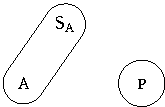
\includegraphics[width=0.3\linewidth]{figures/act_v_alignment}
	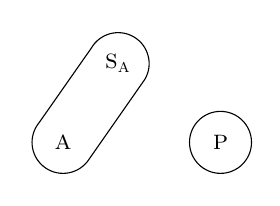
\begin{tikzpicture}
		\topnode{}
		\topleftnode[sa]{\gl{S\textsubscript{A}}}
	%	\toprightnode[sp]{\gl{s_p_}}
		\leftnode[a]{\gl{a}}
		\rightnode[p]{\gl{p}}
		\draw \convexpath{11.2pt}{a,sa};
		\draw (p) circle (11.2pt);
	\end{tikzpicture}
	\caption{Alignment for active verbs}
	\label{fig:alignment}
\end{figure}


\ea\label{ex:itr}
\gll le=soom\\
 3\gl{pl}=swim\\
\glt \qu{They swim.}
\z

\ea\label{ex:an}
\gll le=caihna li=apuli\\
  3\gl{pl}=know \gl{def}.\gl{pl}=person\\
\glt \qu{They know the people.}
\z


\ea\label{ex:stat}
\gll sinu-le\\
 suffer-3\gl{pl}\\
\glt \qu{They suffer.}
\z

%\begin{figure}
%	\centering
%	\begin{tikzpicture}
%	\topnode{}
%	\topleftnode[sa]{\gl{S\textsubscript{A}}}
%	\toprightnode[sp]{\gl{S\textsubscript{P}}}
%	%\leftnode[a]{\gl{a}}
%%	\rightnode[p]{\gl{p}}
%	%\align{sa, sp}
%	\single{sp}
%	\single{sa}
%	\end{tikzpicture}
%	\caption{Alignment for stative verbs}
%	\label{fig:alignment2}
%\end{figure}

%\textit{i sin xhopwen}
%und nicht wenn klar ist, wer gemeint ist

%\ea \ref{ex:v}
% 
% \ili{}{}{} Two active verbs, one in a matrix, one in a relative clause, with the same argument \textit{fati} \qu{speech, word} (B2:94)
% \gll e=holeke nya-si-m li=fati a \textbf{go}=vi
%  1\gl{sg}=receive put-hand-2\gl{sg} \gl{def}.\gl{pl}=speech \gl{rel} 2\gl{sg}=say
% \glt \qu{I gratefully receive from you the words you say}
% 
% \z 
 

A small class of stative verbs are formally indistinguishable from directly possessed nouns, except in that they don't take articles (\sectref{ssec:PossV}). Examples include \textit{mulip} \qu{life} \textit{muliv-am} \qu{you are alive}, \textit{hman-an} \qu{be hungry}.

\begin{table}
	\centering
	\caption{Subject and object markers for active and stative verbs}
	\begin{tabular}{lllll}
	\lsptoprule
		&	Free form	& \gl{a}=/\textsc{s\textsubscript{a}}= & -\textsc{s\textsubscript{p}} & -\gl{p}\\\midrule
		1\gl{sg} & \textit{io} & \textit{e} & \textit{-o(ng)} & \textit{-o} \\
		1\gl{du}.\gl{incl}& \textit{gasu} & \textit{gasu} & \textit{-gasu} & \textit{-kaeu}\\
		1\gl{pl}.\gl{incl} & \textit{gaa/gase} &\textit{ga(se)}&\textit{gaa}&\textit{-kaa}\\
		1\gl{du}.\gl{excl} & \textit{abu} & \textit{abu} & \textit{-abu} & \textit{-(a)bu}\\
		1\gl{pl}.\gl{excl} & \textit{abe}& \textit{abe} & \textit{-abe} & \textit{-(a)be}\\
		2\gl{sg} & \textit{go} &\textit{go} & \textit{-go} & \textit{-ko}\\
		2\gl{du} & \textit{gau} & \textit{gau} & \textit{-gau} & \textit{-kau}\\
		2\gl{pl} &\textit{gavwe}& \textit{gavwe} & \textit{-gavwe} & \textit{-kavwe}\\
		3\gl{sg} & \textit{ia} & \textit{a} & \textit{-(e)a} & \textit{-(e)a}\\
		3\gl{du} & \textit{lu} &\textit{lu} & \textit{-lu} & \textit{-lu}\\
		3\gl{pl} & \textit{le} & \textit{le} & \textit{-le} & \textit{-le}\\
	\lspbottomrule
	\end{tabular}
\label{tab:markers2}
\end{table}


\section{Impersonal verbs}
\label{sec:ZeroTrans}
\is{Verbs!Impersonal verbs}
Impersonal verbs, a term used by \textcite[70]{rivierre_langue_1980} for Cèmuhî, do not take argument indices and cannot occur in the imperative mood, but like other verbs they can form complete clauses by themselves and can either occur with an argument or without it. One subset of impersonal verbs, the affirmative existential \textit{vwa} and the negative existential \textit{cika}, can only take a noun phrase as an argument, but these are not the subject, as evidenced by their inability to take \textit{ka} \qu{\gl{sbj}}. This excludes pronouns. Since Vamale does not have a word for \qu{to have}, having or not having something is expressed with possessive constructions, as in (\ref{ex:vwa_have}): e.g. \qu{there is for me}, calqued into local French: \textit{Il y a une femme pour toi?} \qu{Is there a wife for you?} meaning \qu{Do you have a wife?} \textit{Cika} \qu{\gl{neg}.\gl{exist}} only takes inanimate and non-specific animate arguments, while \textit{cia-} is open to arguments of any animacy, and generic inanimates. \textit{Vwa} \qu{\gl{exist}} may exceptionally take free pronouns and specific animate arguments in marked scenarios (persons will usually be localized with \textit{la} \qu{be here} and demonstratives).

\ea \label{ex:vwa_have}\gll hê tha vwa li=xhaohmu vwa wadala-le\\
 yes \gl{ass} \gl{exist} \gl{def}.\gl{pl}=old \gl{exist} gun-3\gl{pl}.\gl{poss}\\
\glt \qu{Yes, there were elders who had guns.} {[KL:141]} 
\z

Another subset of impersonal verbs takes a complement clause as their sole argument (\ref{ex:impV1}), but can also stand alone (\ref{ex:impV2}). They form a small, closed class, partly derived from nouns. \textit{Goon ma} \qu{allowed, possible to}, \textit{vwasoon ma} \qu{impossible to},\footnote{Maybe from \textit{vwa-s(it)oon} \qu{\gl{exist}-taboo}.} \textit{siteke ma} \qu{forbidden to} work like this (see \Cref{fig:VwaTree}). 
Most members of this class have other meanings when used as nouns or verbs in other contexts, e.g. \textit{goon} \qu{body, enough} but \textit{goon, ma\ldots} \qu{possible, feasible, allowed to\ldots.}


\ea\label{ex:impV1}\gll vwasoon ma go=suu\\
 impossible \gl{comp} 2\gl{sg}=break\\
\glt \qu{You cannot break it.} {[AG1:71]}
\z

\ea\label{ex:impV2}\gll ju-vaa vwasoon\\
 very-too.much impossible\\
\glt \qu{It's too difficult.} {[KG:135]}
\z


%\a
% 
%\ili{}{}{} X10:7
%\gll th=e vwasoon
% \gl{ass}=1\gl{sg} impossible
%\glt \qu{I cannot}
%
%
%\a
%
%\gll *xhwan m=e vwasoon
% almost \gl{subr}=1\gl{sg} impossible
%\glt \qu{(It's almost impossible)}
%

%\ea\label{ex:xhwan}
%
%\ili{}{}{} X10:6
%\gll yo, xhwan ma vwasoon nyakoo-n m=e vwa ena
% 1\gl{sg} almost \gl{subr} impossible for-\gl{nspec} \gl{subr}=1\gl{sg} do \gl{dist} 
%\glt \qu{It's almost impossible for me to do this}
%

%e ra-xhwa thuang me caacaa
%e juu ra caacaa
%*e xhwathuang caacaa
%\qu{i am almost a father}

\textit{Uta} \qu{rain}, \textit{mapeke} \qu{be day}, \textit{bwen} \qu{night} and other members of the lexical field of weather phenomena, sea tide, etc. exist as article-bearing nouns as well, do not take arguments, but can form clauses and take certain adverbs. This third group is called verbs on the basis of constructions where the members cannot behave like typical nouns (\ref{ex:uta}), and following analyses of cognates in other languages, where the forms can be derived to take arguments: \textit{bwen-i-ɛg} \qu{It becomes night around me} \parencite[302]{rivierre_langue_1980}. This argument-taking is not attested in Vamale (anymore), but oblique constructions still exist.



	\ea \label{ex:uta}
		\gll (*i) uta nyako-ong\\
	 \gl{def}.\gl{sg} rain \gl{obl}-1\gl{sg}.\gl{poss}\\
	\glt \qu{It rains on me.}
	\z
	
	\ea	
	\gll thapoke mapeke\\
	 begin bright\\
	\glt \qu{It is (starting to) dawn.}
		\z



%The existential \textit{vwa} and the non-existential \textit{cika} are treated as stative verbs, though they cannot bear subject indices, which is perhaps explainable as a lexical semantic preference. 

%\subsection{vwasoon} %actually maybe not a verb. no agruments.

\begin{figure}
 \begin{forest}
		for tree={
			if n children=0{
				font=\itshape,
				tier=terminal,
			}{},
		}
		[S 
		[V[\textit{vwasoon}]]
		[S'[\textsc{subr}
		[\textit{ma}]]
		[VP
			[PN[\textit{go}{=}]]
			[,shape=coordinate
				[V [\textit{xaleke}]]
				[NP
					[ART[\textit{li}{=}]]
					[N[\textit{mani}]]
				]
			]
		]
		]
		]
	\end{forest}
	\caption{Tree-diagram of the sentence structure of \textit{vwasoon ma go xaleke li mani} \qu{You cannot see the birds}}
	\label{fig:VwaTree}
\end{figure}

%\begin{itemize}
%	\item \textit{vwasoon} \qu{difficult, impossible}
%	\item \textit{goon}\footnote{\textit{hmwagoon} \qu{be equal}} \qu{enough, permitted} this is derived from \textit{goo-n} \textit{body, size; zenith, maximum capacity}
%	\item \textit{vaang} \qu{unknown}
%	\item \textit{vwa} \qu{there is}
%	\item \textit{cika} \qu{there is not}
%	\item \textit{xhwat thuang} \qu{almost} is a fixed expression that takes no nominal argument and needs subordinate, possibly complement clause. it's not a verb since it takes no TAM.
%\end{itemize}
%\todo{are you sure this is only one class? cika wîîn but ?goon wîîn}

%\textit{Vwasoon} and \textit{goon} need a subordinator afterwards, which seems to be a clue that they do not take arguments. They are probably derived from nouns. \textit{goo-n xat} \qu{midday} looks like a classic possessive construction, literally \qu{enough sun} in the modern language, maybe \qu{maximal sun} before, because \textit{goon} is mostly used for \qu{enough, no more!} as a threat or plea, if it does not occur in the formula \textit{goon ma X...} \qu{it is possible/good...} (asking for permission or asking somebody to do something). \textit{Goon} also means \qu{body}. In the same sense, considering that the first syllable in \textit{vwasoon} \qu{impossible} only ever occurs as the morpheme \textit{vwa} \qu{exist; do}, this may be an old VP, lexicalized but still, following the "there is X" pattern, needless of arguments.
%\textit{Cika} \qu{\gl{neg}.\gl{exist}} is the same class as \textit{vwa} \qu{\gl{exist}}. They both take an argument, which can be implied if already mentioned.

 \section{Stative verbs}
\label{sec:StatV}
\is{Verbs!Stative verbs}

``Stative verbs" are a classic feature in New Caledonian languages, already described in \textcite{haudricourt_langues_1948}, and descend from Proto-Oceanic \parencite[63]{lynch_oceanic_2002}.\footnote{\citeauthor{lynch_oceanic_2002} distinguish stative and dynamic verbs, while the French tradition, and this study, call the latter ``active" verbs.} They are inflected with morphemes that closely resemble postponed free forms, as in \tabref{tab:hmet}. Like the undergoers of transitive verbs, the animacy of the referent decides whether the subject of a stative verb is marked: inanimate participants are not indexed on the verb.

\begin{table}
	\caption{Inflection of \textit{hmet-} \qu{sated}}
	\begin{tabular}{lll}
		\lsptoprule
\gl{sg} & 1 &\textit{hmet-eo}\\
		&2& \textit{hmet-go}\\
		&3& \textit{hmet-ea}\\
		\midrule
\gl{du} & 1\gl{incl}& \textit{hmet-gasu}\\
		&1\gl{excl}&\textit{hmet-abu}\\
		&2&\textit{hmet-au}\\
		&3& \textit{hmet-lu}\\
		\midrule
\gl{pl} & 1\gl{incl}& \textit{hmet-gaa}\\
		&1\gl{excl} & \textit{hmet-abe}\\
		&2 & \textit{hmet-gavwe}\\
		&3 & \textit{hmet-le}\\
		\lspbottomrule
	\end{tabular}
	\label{tab:hmet}
\end{table}

Stative verbs are a closed class, semantically vaguely characterized by a patientive S (though many active verbs also have a patientive S, e.g. \textit{weke} \qu{to be angry}, or \textit{khûda} \qu{to stink}). The argument is marked in the same position as transitive undergoers, and shares the latter's form, except in the first and second persons, where P arguments have a devoiced form, i.e. \textit{-ko} \qu{2\gl{sg}}, \textit{-kaa} \qu{1\gl{pl}.\gl{incl}} etc. This means that S is marked in two ways: S and A are marked the same for active verbs, and stative verb S subjects are either marked the same as P, or slightly differently, depending on the speaker and the verb. We thus have a tripartite system, though stative S and P are merged by many younger speakers, yielding a split-intransitive system like in western Voh-Koné. Diachronically, stative S and P participants were probably expressed as free pronouns following the predicate (V PN),\footnote{This may be linked to a Proto-Oceanic VSO or VOS word order \parencite[86, 87]{lynch_oceanic_2002}, though nowadays SVO is more widespread and considered canonic \parencite[49]{lynch_oceanic_2002}. Note that this would not explain the indexing found on active verbs.} which became incorporated into the verb (e.g. \textit{hmwet ia} \qu{tired 3\gl{sg}} $\rightarrow$ \textit{hmwet-ea}). Indirect possession underwent a similar process (\textit{thala-n ia} \qu{knife-\gl{poss} 3\gl{sg}} $\rightarrow$ \textit{thala n-ea}). 
The stative verb \textit{hmana-n} \qu{be hungry} (not a noun because it cannot take an article) has the paradigm of a directly possessed noun, and shares this property with \textit{muliva-n} \qu{be alive} (see \sectref{ssec:PossV}).

%\begin{itemize}
%	\item \textit{yamaan}\qu{be not motivated} 
%	\item \textit{saxhwe} \qu{refuse to eat} is actually just stative
%	\item \textit{sahnaang} \qu{not understand} is also just stative
%\end{itemize}


\subsection{Dependent stative verbs}
\label{ssec:Verbs_n}
\is{Verbs!Stative verbs!Dependent stative verbs}
Some verbs, active as well as stative ones, show nominal inflection. This grammar will use the term \textsc{dependent verb} found in some New Caledonian descriptions \parencite[207]{ozanne-rivierre_iaai_1976} for these verbs that can index a non-specific argument with a generic \textit{-n} (similarly to inalienably possessed nouns, called \textsc{dependent nouns} in the French tradition, which also cannot omit marking their modifier). Active verbs with nominal morphology work rather differently and are discussed in \sectref{ssec:active-n}. The verbs described here take different subject-indexing suffixes depending on animacy and specificity of the subject, as shown in \Cref{tab:V-n}. There are few still productive verbs in this category, but they are frequently used. Common members include \textit{xhopwe-n} \qu{grow/be big}, \textit{xhwati-n} \qu{be small}, \textit{hmai-n} \qu{be many}, \textit{sate-n} \qu{be different}, \textit{yape-n} \qu{be old (inanimate)}. % This section will use \textit{xhopwe} as an example.%, \textit{e-n} \qu{be first}. 


Animate subjects are indexed on stative verbs with personal suffixes (\textit{-eo} \qu{1\gl{sg}}, \textit{-go} \qu{2\gl{sg}} etc.) when they are not present as a noun phrase (\ref{ex:Vn1}). Inanimate subjects take \textit{-n} \qu{\gl{ana}} in these cases (\ref{ex:Vn2}). %If the subject is expressed as an NP in the same clause, the stative verb does not carry a suffix for animate NPs (\ref{ex:VnbareAnim}), and definite inanimate NPs (\ref{ex:VnbareInanim}). 

\ea\label{ex:Vn1}
\gll sate-o\\
 different-1\gl{sg}\\
\glt \qu{I am different.}
\z


\ea\label{ex:Vn2}
\gll sate-n (koo-n)\\
 different-\gl{ana} (\gl{obl}-\gl{ana})\\
\glt \qu{It is different (from it).}
\z

Generic subjects are always marked with \textit{-n} \qu{\gl{nspec}} (\ref{ex:Vn}). These rules begin to be less rigidly enforced in Voh-Koné languages in general \parencite[51]{rivierre_bwatoo_2006}, and \textit{-n} now often appears before noun phrases regardless of their animacy and specificity (\ref{ex:xhopwen i-X}). This may have contributed to the development of noun phrase internal modifiying verbs (see \sectref{sec:adj}).
\ea\label{ex:Vn}\gll e=vi hapi na naen xadaa sate-n \\
 1\gl{sg}=say \gl{comp} \gl{dem} now on.the.other.hand different-\gl{nspec}\\
\glt \qu{I'm saying that now things have changed.} {[KL:243]}
\z

Some stative verbs have split into two forms with different meanings, e.g. \textit{hmwaka-n}, \textit{hmwaka-o} \qu{be like it, be like me}, but \textit{hmwakan} \qu{maybe}.
Verbs with nominal morphology can also be found in Cèmuhî \parencite[179, 183]{rivierre_langue_1980} and Nyelâyu \parencite[48]{ozanne-rivierre_nyelayu_1998}. They are not described as an open class in these grammars. Though most verbs with nominal morphology in Vamale are stative, there are also active ones. A prominent example is \textit{caihna-n} \qu{to know} (discussed in more detail \sectref{ssec:active-n}). Some stative verbs with \textit{-n} can be derived with \textit{-ke} \qu{\gl{tr}}, compare \textit{xhwatii-n} \qu{be small} and \textit{xhwatii-ke} \qu{do softly}.







\begin{table}
	\caption{Meanings of \textit{xhopwe-} \qu{grow}}
	\begin{tabular}{lll}
	\lsptoprule
		1\gl{sg}	&\textit{xhopwe-o}& \qu{I grow}\\
		2\gl{sg}	&\textit{xhopwe-go}& \qu{You grow}\\
		3\gl{sg}&\textit{xhopwe-a}& \qu{S/He grows}\\
		\gl{nspec}& \textit{xhopwe-n} & \qu{It is big}\\
		overt NP & \textit{xhopwe} & \qu{It is bigger than X/before}\\
	\lspbottomrule
	\end{tabular}	
	\label{tab:V-n}
\end{table}

For \textit{xhopwe-n} \qu{big}, there is a meaning distinction along an animacy axis: without \textit{-n}, it expresses either a development \qu{big} $\rightarrow$ \qu{get bigger}, through time in comparison with an earlier state (\qu{grow}), or synchronically in comparison with others (\qu{be bigger than}, see example \ref{ex:VnAnim}). A table summarizes the forms (\Cref{tab:V-n}). \textit{xhopwe-} means \qu{to be bigger} for animate subjects (\ref{ex:VnAnim}) and \qu{to be big} for inanimates (\ref{ex:xhopwen i-X}, \ref{ex:xhopwen}). %, if it is clear from the context that it is a momentary observation. %\textit{xhopwe-} means \qu{to grow, to be bigger} for all subjects (\ref{ex:VnbareInanim}, \ref{ex:xhopwen can}). 


\ea\label{ex:VnAnim}\gll 	i=apuli a= xhopwe-a (koo-le)\\	
	\gl{def}.\gl{sg}=man \gl{rel}= big-3\gl{sg}.\gl{S\textsubscript{P}}	(\gl{obl}-3\gl{pl})\\
	\glt	\qu{the bigger man (in years, status, size) (than them)}	\\
\z

\ea\label{ex:xhopwen i-X}
\gll 	xhopwe(n) i=goon	\\
	big	\gl{def}.\gl{sg}=body\\
\glt	\qu{the big body (height, corpulence)}
\z
%\a
%
%\gll 	*xhopwen goon	
%	big body	
%%\glt	personne de grande taille	
%
%\a\label{ex:VnbareInanim}
%
%\ili{}{}{} \textit{xhopwe-n} and other verbs denoting amount, size, length etc take comparative meaning in appropriate settings.
%\gll 	xhopwe i si-n mo-ko i s-ung	
%	big \gl{def}.\gl{sg}=hand-3\gl{sg}.\gl{poss} more.than \gl{def}.\gl{sg}=hand-1\gl{sg}.\gl{poss}	
%\glt	\qu{His hand is bigger than mine}	
%

%\textit{xhopwen} in (\ref{ex:xhopwen i-X}) means \qu{its growth, its size}, and is derived from \qu{to grow}. Compare \textit{hun-xhopwen an}, literally \qu{his/her way of being/becoming big} means \qu{his/her corpulence}. % %todo{??? What is exactly derived from what here...?} 
%though
%Syntactically, \textit{xhopwen} is used similarly to \textit{joaka-n}, as shown in \Cref{tree:joakan}, .
A construction frequently seen with animate subjects is shown in (\ref{ex:xhopwen}). The unmarked use of \textit{xhopwe}, as explained above, is as a predicate with comparative meaning (\ref{ex:VnbareAnim}). In a relative clause, \textit{xhopwe} is ungrammatical without a resumptive subject-indexing suffix (\ref{ex:Vno}), e.g. \textit{-a}, or an anaphoric suffix \textit{-n} (\ref{ex:xhopwen can}). In example (\ref{ex:xhopwen}), however, the meaning of \textit{xhopwen} is not comparative. This construction seems to be a strategy to avoid the incremental\slash comparative meaning of certain stative verbs, and may be related to the de\hyp grammaticalization of \textit{-n} mentioned for \textit{xhopwen} in \Cref{tab:V-n}.


\ea[]{\label{ex:xhopwen}
%\ili{}{}{} This seems to be an expression, where the \textit{-n} refers not to the man, but to his body.
\gll 	i=apuli a= xhopwe-n\\
	\gl{def}.\gl{sg}=man \gl{rel}= big-\gl{ana}	\\
\glt	\qu{the fat/old/important man}}
\z


\ea[]{\label{ex:VnbareAnim}
\gll 	xhopwe i=apuli-aen	\\
	grow \gl{def}.\gl{sg}=man-\gl{dem}	\\
\glt	\qu{This man is bigger/taller/ more important.}}
\z

\ea[*]{\label{ex:Vno}
\gll 	i=apuli a= xhopwe\\
	\gl{def}.\gl{sg}=man \gl{rel}= big	\\
\glt	(for: \qu{the man who is big})}
\z

\ea[]{\label{ex:xhopwen can}\gll 	i=apuli a= xhopwe-n ca-n dawee-lu	\\
	\gl{def}.\gl{sg}=man \gl{rel}= big-\gl{ana} in-\gl{nspec} between-3\gl{du}.\gl{poss}	\\
\glt	\qu{the fatter man of the two}}	
\z

	%\a
	%
	%%% \ili{}{}{} 
	%\gll 	*si-n xhopwen	
	%		
	%\glt		
	%
	
	%\a
	%
	%%% \ili{}{}{} 
	%\gll 	si-n a xhopwen	
	%	hand-3\gl{sg}.\gl{poss} \gl{rel} big	
	%\glt	\qu{(The) hand which is big}
	%
%	\z
	
%\end{multicols}


%\begin{table}
%	\label{tab:V-n}
%	\caption{V-n}
%\begin{tabular}{lllll}
%
%Verb & \gl{def} hand & \gl{indf} hand & \gl{def} man & \gl{indf} man\\
%\midrule
%xhopwe \_ & the hand is big & * & the biggest & an elder\\
%vaa xhopwe \_ & the biggest hand& * & the biggest & an elder\\
%%\_ a xhopwe & * & * & * & *\\
%%\_ xhopwe & * & * & * & *\\
%xhopwen \_ &the big hand &* &* &*\\
%%xhopwen \_ & & *vuki yee &&\\
%\_ a xhopwen & the big hand & size & the big man & a big man\\
%\_ xhopwen & i sin & sin & size & size \\
%\_ a kon xhopwen & i sin & sin & * & * \\
%%\midrule
%xhopwea\_ & * & * & he gets fatter & *\\
%\_ a xhopwea & * & * & the elder/biggest & the elder/biggest \\
%\_ xhopwea & &&elder&elder \\
%\_ a kon xhopwea & * & * & growing&\\
%\_ a kon xhopwen & & & growing? & \\
%\midrule
%cie\_ & * &* & i/eca apuli & *\\
%\_ cie-a & * & * & the/some man is absent & *\\
%cian & the hand is not there&*&*&* \\
%\end{tabular}
%\end{table}

%Hypothesis: animacy plays a role, it's not productive anymore (otherwise daahma a xhopwen would not work) or xhopwen is special.


\subsection{Numerals}
\label{ssec:Numerals}
\is{Numerals}
\is{Verbs!Numerals}

Numerals in Vamale are stative verbs that can take subject suffixes, as \Cref{tab:numbers} shows. Some are derived from nouns, notably 5 from \qu{hand}\footnote{From \textit{si-} \qu{hand}, showing the tendency to rather speak of 2\gl{sg} or 1\gl{pl}.\gl{incl} than an indefinite 3\gl{sg}.} and 20 from \qu{person}, the bases of the system. Complex numerals used to be formed like clauses, made of coordinated verb phrases. 

%\begin{minipage}{\textwidth}
\begin{table}
	\centering
\caption{The first six cardinal numerals and their verbal form}
\begin{tabular}{llll}
\lsptoprule
Number & Gloss & Suffixed form & Gloss\\\cmidrule(r){1-2}\cmidrule(l){3-4}
\textit{se}& \qu{1}& \textit{see-a} & \qu{s/he is one, s/he is alone}\\
\textit{thalo(o)}& \qu{2} & \textit{thaloo-lu} & \qu{they are two}\\
\textit{thi(i)en}& \qu{3} & \textit{thien-le} & \qu{they are three}\\
\textit{fava}& \qu{4}& \textit{fava-le} & \qu{they are four}\\
\textit{nim} & \qu{5}& \textit{nim-le} & \qu{they are five}\\
\textit{nim a bwa se}& \qu{6}& \textit{nim a bwa see-le} & \qu{they are six}\\
\lspbottomrule
\end{tabular}
\label{tab:numbers}
\end{table}
%\end{minipage}


 \textit{(N)a-bwa} was only recorded with complex numerals, some of which are shown in \Cref{tab:compo_numbers}. The initial nasal only occurs if the preceding element ends in an open syllable. Bwatoo has \textit{bwa} as \qu{+} \parencite[45]{rivierre_bwatoo_2006}, maybe related to \textit{pwa} \qu{on} or \textit{bwa}- \qu{head}. Leenhardt translates \textit{vajilu ka bwa nim ka bwa se} \qu{16}, then with \textit{ka} instead of \textit{na}, as \qu{ten and the right hand raised and open, and the thumb sticking out of the fist}, but no modern Vamale word would tie \textit{bwa} to either palm (\textit{yataan}), fist (\textit{daamuun}) nor the right hand (\textit{juu sin}) \parencite[166]{leenhardt_langues_1946}. The element having replaced the coordinator \textit{ka} is another puzzle. The demonstrative pronoun \textit{na} often means \qu{It is X (who did/is Y)}, and may have replaced the former coordinator \textit{ka} \parencite[166]{leenhardt_langues_1946} in a sense of `five, this on top of two' for \qu{7} (\ref{ex:7}). This grammar writes the coordinator \textit{na-bwa} joined by a hyphen to account for its single stress contour.
 
\ea \label{ex:7}
 \gll nim (a)-bwa thaloo\\
	  5    plus   2\\
 \glt \qu{7}\\
 \z 

\begin{table}
	\caption{Complex numerals}
	\begin{tabular}{ll}
	\lsptoprule
		\textit{vajilu na-bwa nim a-bwa se} & \qu{16}\\
		\textit{thaloo vajilu} & \qu{20}\\
		\textit{se apuli} \textit{na-bwa nim a-bwa se}& \qu{26}\footnote{\textit{se apuli} lit. \qu{one person}}\\
		\textit{se apuli na-bwa vajilu}& \qu{30}\\
		\textit{thaloo apuli}& \qu{40} (arch.)\footnote{This is never given spontaneously. People are mentally in a ten-based system now (see the word for 20).}\\
		\textit{nim apuli}& \qu{100} \\
		\textit{apuli ko apuli} & \qu{400}\\
	\lspbottomrule
	\end{tabular}
	\label{tab:compo_numbers}
\end{table}

\textit{Vajilu} \qu{10} could be etymologically composed as in (\ref{ex:10}). The last syllable is likely \textit{-lu} marking 3\gl{du}.\gl{poss} on nouns. The system being 5-and 20-based as is typical of the region \parencite[261]{haudricourt_dictionnaire_1982}, and finally \textit{Iaai} saying \qu{two hands} for 10, maybe the etymology of this word is something like in (\ref{ex:10}), but this is purely speculative.

\ea \label{ex:10}
\gll vwa si-lu\\
 \gl{exist} hand-3\gl{du}.\gl{poss}\\
\glt \qu{They have hands/there are their hands.}
\z 

According to \textcite[45]{rivierre_bwatoo_2006}, and also Dego Philippe Gohoupe, another word for 100 is \textit{se apuli} \qu{one person}. This confusing polysemy makes more sense considering that the Pacific Franc used to have a 100 Franc bill with a man on it (see \Cref{fig:100CFP}), was a salient thing, and spoken about much more often than groups of twenty. Nowadays, saying \textit{se apuli} normally means \qu{100}, but \textit{se apuli na bwa se} is \qu{21}, whereas \textit{nim apuli} is \qu{100} if it is part of a complex numeral. Leenhardt notes \textit{nilu apuli} for \qu{100} without glossing it \parencite[166]{leenhardt_langues_1946}{}. Whether \textit{nim apuli} is interpreted as 500 or 100 is difficult to ascertain, since most speakers are unsure. Vamale numerals are rarely used beyond 5 in the language, while French loans are taking over due to school, money, hours of the day, and a decay of counting contributions in customary ceremonies. Multiplying based on 20 is attested in \citetitle{leenhardt_langues_1946} for most languages, amongst which is Hmwaveke with \textit{sec apulip ko apulip} for 400, literally \qu{one person on people, or \qu{20 on 20}}, which suggests, along with \textit{nim apuli} \qu{100 (lit. 5 20)}, that the multiplication base comes last, and the multiplier first \parencite{leenhardt_langues_1946}. 

\begin{figure}
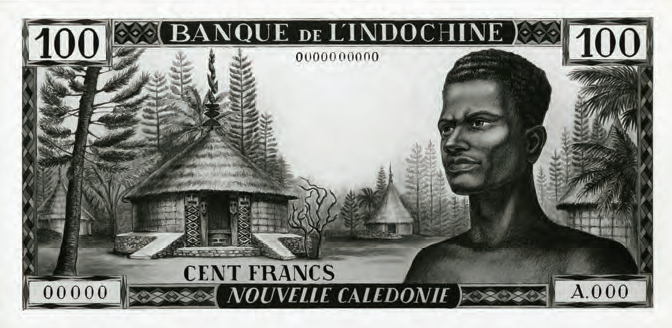
\includegraphics[width=\linewidth]{figures/100_francs}
\caption{A 100 CFP bill from 1964 \parencite[24]{ieom_lhistoire_2014}}
	\label{fig:100CFP}
\end{figure}
 
\subsubsection{Ordinals}
\is{Ordinals}
\is{Verbs!Ordinals}
\largerpage

Ordinals are formed with \textit{e-}\footnote{\textit{bɛ-} in Cèmuhî, used only with ordinals  \parencite[271]{rivierre_langue_1980}.} and \textit{(k)a-n} \qu{\gl{clf}.\gl{poss}-\gl{nspec}},\footnote{The Cèmuhî cognate [hɛ̃̀] is analyzed as a possessive morpheme by Rivierre \parencite[271]{rivierre_langue_1980} and otherwise only present in part-of-whole compounds.} yielding the forms listed in \Cref{tab:ordinal}. Leenhardt (1946) recorded irregular forms which have now disappeared, \textit{i a vathabun} \qu{the first (lit. s/he who is in front)},\footnote{Leenhardt's \textit{vathabun} is \textit{pa(a)thabun} nowadays.} now regular \textit{i e-se=kan} \qu{the first}, and \textit{i ethice nawe},\footnote{Since the clitic \textit{=(k)a-n} is used for possessum classifying purposes elsewhere, Leenhardt's form could have been \textit{i e-thicen=a-vwe}, with -\textit{vwe} \qu{2\gl{pl}.\gl{poss}}.} now \textit{i e-thien=an}. They, too, are rarely used beyond 5.

\begin{table}
	\caption{Ordinals}
	\begin{tabular}{ll}
	\lsptoprule
		\textit{(i) e-se kan} & \qu{(the) first}\\
		\textit{i e-thalo kan} & \qu{the second}\\
		\textit{i e-thien an} & \qu{the third}\\
		\textit{i e-fava kan}&\qu{the fourth}\\
		\textit{i e-nim an}&\qu{the fifth}\\
		\textit{i e-vajilu na bwa nim na bwa se kan}&\qu{the sixteenth}\\
		\textit{i e-koin an}& \qu{the last}\\
	\lspbottomrule
	\end{tabular}
	\label{tab:ordinal}
\end{table}

Ordinal numbers seem to have lexicalized \textit{ka-n} \qu{\gl{clf}.\gl{poss}-\gl{nspec}}, since it cannot be omitted. Onto it, another \textit{ka} can be added (but does not necessarily have to be) in order to make it possessible by the noun \textit{en} \qu{moment} (\ref{ex:kan en}, \ref{ex:kan en2}).

\ea \label{ex:kan en}\gll ja i={\ob}e-thalo-kan ka-n en{\cb} a tipwa\\
 \gl{prf} \gl{def}.\gl{sg}=\gl{ord}-two-\gl{link} \gl{clf}.\gl{poss}-\gl{nspec} moment \gl{rel}.3\gl{sg} fall\\
\glt \qu{It is the second time that it falls.} {[JN1:21]}
\z


\ea \label{ex:kan en2}
%\ili{\textit{ja iekoinan kan en exaleko}}\\
\gll ja i=e-koin-an ka-n en a= e=xale-ko\\
 \gl{prf} \gl{def}.\gl{sg}=\gl{ord}-end-\gl{link} \gl{clf}.\gl{poss}-\gl{nspec} moment \gl{rel}= 1\gl{sg}=see-2\gl{sg}.\gl{obj}\\
\glt \qu{It is the last time that I saw you.} {[JN1:36]}
\z


\subsubsection{Multiplicative \textit{o}}
\is{Numerals!Multiplicative}

The multiplicative prefix \textit{o-} (\qu{X times}) only occurs with numerals. The resulting word is derived to an adverb (\ref{ex:o-thiien}). Hence, multiplicatives cannot be predicates in a matrix clause, but do occur in adjunct clauses. Exceptions are interjections like the work call \textit{o-see!} \qu{do at once, in one hard pull}. \textit{O} \qu{X times} is analyzed as a prefix as well in Nêlêmwa \parencite[39]{bril_nelemwa_2002} and Bwatoo (where it is \textit{we-}) \parencite[46]{rivierre_bwatoo_2006}. In (\ref{ex:hunmata}), however, the adverb is possessed by a third person. I analyze this as a zero derivation.

\ea\label{ex:o-thiien}
\gll a=tho nyakoo-m \textbf{o-thiien} \\ %\textsubscript{Adjunct}
 3\gl{sg}=call \gl{obl}-2\gl{sg}.\gl{poss} times-three\\
\glt \qu{S/he called you three times.} {[2019-08-05 JP ka 42.1]}
\z


\ea\label{ex:hunmata}\gll pa ja o-thien-n-ea ko i=(hun-) mata\\
 \gl{prf} \gl{prf} times-three-\gl{poss}-3\gl{sg}.\gl{poss} \gl{obl} \gl{def}.\gl{sg}=\gl{nmlz}- sing\\
\glt \qu{This is the third time that he sings.} {[vamale-181127-jp\_nelemwa-1: 00:11:51-00:11:52]}
\z


%\ea
%\begin{multicols}{2}
%	\a
%	
%	\ili{}{}{} PE1:22.1 Is this really the same?
%	
%	\gll {[}{[}nim-ambwa-see]\textsubscript{V} o]\textsubscript{Adverbial Clause} {[}hun-bita-eo]\textsubscript{NP}
%	
%	 5-plus-1 times \gl{nmlz}-turn-1\gl{sg}
%	
%	\glt \qu{6 times I turned}
%	
%	
%	
%	
%	\a
%	
%	\gll nim-ambwa-see\textsubscript{V} o hun-bita-eo
%	
%	 5-plus-1 \gl{irr} \gl{nmlz}-turn-1\gl{sg}.\gl{poss}
%	
%	\glt \qu{Six would be my turns}
%	
%	
%\end{multicols}
%\z
%\todo{listen to the recording} 


\subsection{Possessible verbs}
\label{ssec:PossV}
\is{Verbs!Possessible verbs}

``Possessible verbs" are distinguished here from ``verbs with \textit{-n}", though they both carry a morpheme \textit{-n} in the third person, because the latter inflect using stative subject indexing suffixes (including \textit{-n} \qu{\gl{nspec}}), and the former take possessive morphology (including \textit{-n} \qu{3\gl{sg}.\gl{poss}}, see \Cref{tab:poss}). There are two subsets of stative possessible verbs, one with alienable and one with inalienable possessive morphology. 
Inalienably possessed intransitive verbs, such as the ones below (\ref{ex:hman1}), are not transparently derived from nouns (\ref{ex:hman3}), with the exception of \textit{nyima-} \qu{heart} \goodtilde \qu{to want}. Nouns can be derived from some of them using typical deverbal constructions (\ref{ex:xhopwen i}).
\begin{enumerate}[(a)]
\item \textit{hman-ong} \qu{I am hungry}, \textit{hmana-n}  \qu{s/he is hungry}
\item \textit{bwaa-ng}, \textit{bwaa-n}, \textit{bwaa-ju} \qu{if only}. This has an interjection counterpart \textit{bwaa-m} \qu{poor/darling you!}. Since this item cannot take an article and can stand as clause, it is analyzed as a verb.
\item \textit{holoo-m}, \textit{holoo-u}, \textit{holoo-vwe} \qu{goodbye (you, you two, you all)}
\item \textit{nyim-ong} \qu{I want, like}
\item \textit{vwaseek-ong} \qu{I am sad}
\end{enumerate}


	
	\ea\label{ex:hman1}
	% \ili{}{}{} \textit{hmanong}, \textit{hmanam}, \textit{hmanan}
	\gll hman-ong\\
	 hungry-1\gl{sg}.\gl{poss}\\
	\glt \qu{I am hungry.}
	\z
	% *i sinuong %that's just a normal stative verb, what the fuck
%	\ea\label{ex:hman2}
%	
%	\gll *i=hman
%	 \gl{def}=hunger
%	\glt (for: \qu{The hunger})
%	
	
	 \ea\label{ex:hman3}
	     \textit{*i=hman-an} (for: \qu{his/her hunger})
	\z
	
	\ea\label{ex:xhopwen i}
	\gll paa juu va xhopwen i=hun-hman-ong\\
	 already really too big \gl{def}.\gl{sg}-\gl{nmlz}-hungry-1\gl{sg}(.\gl{poss})\\
	\glt \qu{I am more and more hungry.} (lit. \qu{My hungering has become really big})
\z
	% \a
	% 
	% \gll i=nyai-n
	%  \gl{def}=offspring-3\gl{sg}.{poss}
	% \glt \qu{his/her child {[}inalienable]}
	% 
	


There are few alienably possessed intransitive verbs. They include \textit{yamaan-eong}, \textit{yamaan-ea}, \textit{yamaan-gasu} \qu{be unwilling to do for lack of motivation, be fed up with something}, and \textit{saxhwe-ong}, \textit{saxhwe-a} \qu{refuse to do},\footnote{This possibly contains the morpheme \textit{xhwe} \qu{be across}.} as well as \textit{yathô-ong}, \textit{yathô-a} \qu{be in a hurry}. \textit{Sinu-ong}, \qu{be sick, be suffering; die} also exists as a noun meaning \qu{illness}. % is indistinguishable from stative verbs except in the first person, there is some flexibility.
Possessible verbs, mostly verbs with an Undergoer argument, take possessive morphology usually found on nouns, but cannot bear an article. They are intransitive, like all stative verbs. The second subset, with alienable possessive morphology, could be derived from the very similar stative paradigm, and in many cases the subject-indexing suffixes differ between speakers: \textit{sino-ong} \goodtilde \textit{sinu-o} \qu{ill-1\gl{sg}}, \textit{saxhwe-ong} \goodtilde \textit{saxhwe-o} \qu{refuse-1\gl{sg}}.

 \section{Active verbs}
 \label{sec:ActV}
 \is{Verbs!Active verbs}
Active verbs, the biggest group of verbs, have transitive and intransitive members, and many of them are ambitransitive, meaning they can take an object, but do not have to. As is common in Oceanic languages \parencite[510]{ross_morphosyntactic_2004}, there are no ditransitive verbs in Vamale. This section will first introduce transitive verbs, with their suffixes \textit{-i} and \textit{-ke}, then describe transitive verbs with nominal inflection (called \qu*{dependent} transitive verbs), before addressing transitive verbs that require a preposition \textit{ko-} \qu{on}.

Active intransitive verbs are formally not distinct from transitive verbs, except in that they do not take object suffixes. This is in line with Proto-Oceanic \parencite[81]{lynch_oceanic_2002}. Both transitive (e.g. \textit{vavi} \qu{hunt something}) and ambitransitive verbs (e.g. \textit{xaahni} \qu{check, stare (at)}) can occur without an argument, before other (ad)verbal elements of the verb phrase, or with a generic argument, and will still carry transitive suffixes \textit{-i} or \textit{-ke}, discussed below. Purely intransitive ones usually do not end in \textit{-i} or \textit{-ke}, see (\ref{ex:intrV}). All active verbs take subject marking bound pronouns, as in examples (\ref{ex:index_actV}) and (\ref{ex:index_actV2}). \Cref{tab:markers2} lists the bound pronouns.

\ea \label{ex:intrV}\gll tabo tabo li=xho thamo, thêên thêên li=xho xayu\\
 sit sit \gl{def}.\gl{pl}=cicada female fly fly \gl{def}.\gl{pl}=cicada male\\
\glt \qu{Sit sit oh female cicadas [full of eggs], fly fly (away) oh male cicadas.} (children's song, female cicadas bear eggs and are tastier) {[children's song]}
\z

\ea \label{ex:index_actV}\gll \textbf{e}=han-mwa ko-m=\textbf{e} vwa ma=\textbf{a} thuup ka i=jamw-ong\\
 1\gl{sg}=go-\gl{rep} because-\gl{subr}=1\gl{sg} do \gl{comp}=3\gl{sg} bathe \gl{sbj} \gl{def}.\gl{sg}=father-1\gl{sg}.\gl{poss}\\
\glt \qu{I'm going back to make my father take a bath.} {[PQ 10.1]}
\z


\ea \label{ex:index_actV2}\gll tha=\textbf{abe}=vataan fai li=ya-be. cahma li=mama-n-abe, \textit{non}. tha=\textbf{le} fwi-kabe ma=\textbf{abe}=mu bwa e-nyoot\\
 \gl{ass}=1\gl{pl}.\gl{excl}=each cook \gl{def}.\gl{pl}=starchy.food-1\gl{pl}.\gl{excl} concerning \gl{def}.\gl{pl}=mother-\gl{poss}-1\gl{pl}.\gl{excl} no \gl{ass}=3\gl{pl} pinch-1\gl{pl}.\gl{excl}.\gl{obj} \gl{subr}=1\gl{pl}.\gl{excl}=\gl{freq} \gl{ipfv} \gl{refl}-wake.up\\
\glt  \qu{We'd cook our own lunch. Our mothers however, no. They'd pinch us so that we'd wake up.} {[PE2:50]}
\z

\subsection{Transitive verbs}
\label{ssec:TransV}
Transitive verbs mark the subject at the beginning and the undergoer object (if animate, but this condition is disappearing) at the end (\ref{ex:actV}).\footnote{In example \REF{ex:actV}, the subject marker was omitted. This may be due to the elicitation context, where there no referent for the chaser was established. } There are no ditransitive verbs; non-core arguments such as recipients, goals, experiencers and stimuli (depending, of course, on the verb) are marked with the oblique markers \textit{nyasi-} and \textit{nyako-} (see \sectref{sec:oblique}). The transitive verb \textit{holeke} \qu{thank, receive}, for example, has the Theme as a direct object and the Recipient is added through \textit{nyako}- or \textit{nyasi}- (\ref{ex:nyasi_bofukaje}). \textit{nyasi}- is more polite and can only be used with humans. Transitive verbs almost invariably appear with the now lexicalized transitive suffix \textit{-i}, \is{Transitivity!Transitive \textit{-i}}\is{Transitivity!Transitive \textit{-ke}}possibly descended from Proto-Oceanic \textit{*-i} \parencite[507]{ross_morphosyntactic_2004}, or with the still productive \textit{-ke}, possibly descended from \textit{*-akin(i)} \parencite[507]{ross_morphosyntactic_2004}. \sectref{ssec:ke_i} describes this in more detail. Transitive verbs without these suffixes are e.g. \textit{tua} \qu{detach}, \textit{tuu} \qu{take something out of somewhere}, \textit{sivu} \qu{blow; smoke}.

\ea \label{ex:actV}\gll (a=) ha-me wati-ko ko go=imwi i=nyai-n\\
 3\gl{sg}= go-\gl{dir.cp} chase-2\gl{sg}.\gl{obj} because 2\gl{sg}=grab \gl{def}.\gl{sg}=child-3\gl{sg}.\gl{poss}\\
\glt \qu{It comes to chase you because you took its pup.} {[B2:36]}
\z

\ea \label{ex:nyasi_bofukaje}\gll gaa=se-me holeke \textbf{nyasi} bofukaje i=thoatit-ca a= tha=a=bwa nya si-je\\
 1\gl{pl}.\gl{incl}=together thank \gl{obl} god \gl{def}.\gl{sg}=day-\gl{dem}.\gl{prox} \gl{rel}= \gl{ass}=3\gl{sg}=\gl{ipfv} put \gl{ben}-1\gl{pl}.\gl{incl}\\
\glt \qu{We all thank God together for this day that he gave us.} {[Adèle Gohoupe's Song ``Hole Nyasi Daahma":1]}
\z 



%\ex 
%
%\ili{}{}{} GD:12
%\gll  ma xa-wekee-go, go feana-ke ca wîî-m, go hân cabi doop! e=bo \textbf{cade-ko}, go eca apuli
%
% \gl{subr} \gl{agt}.\gl{nmlz}-rage-2\gl{sg}, 2\gl{sg} show-\gl{appl} \gl{indf}.\gl{pl} strength-2\gl{sg}.\gl{poss}, 2\gl{sg} go crush soil 1\gl{sg} \gl{irr} admire-2\gl{sg}.\gl{obj} 2\gl{sg} \gl{indf}.\gl{sg}=person
%
%\glt \qu{If you are enraged, show your strength, go break{ [=}till] some earth ! {[Then]} I shall admire you, {[}if] you are a man.}
%
%
%\z

\subsubsection{Transitive suffixes \textit{-ke} and \textit{-i}}
\label{ssec:ke_i}
\is{Transitivity!Transitive \textit{-ke}}
The transitive suffix -\textit{ke} is the only productive transitive suffix in Vamale. This grammar calls \textit{-ke} a transitive rather than applicative suffix because it does not routinely turn obliques into direct objects, but can derive transitive from intransitive verbs, or even transitive verbs from complex verbs and nouns. Furthermore, and perhaps most importantly, the suffix is in complementary distribution with an object marker: \textit{-ke} appears if the animate object is not overt, as in examples (\ref{ex:ke_noke1}) and (\ref{ex:ke_noke2}). This distiguishes \textit{-ke} from \textit{-i}, which is part of the stem and cannot be replaced.\footnote{Contrary to the Vamale form \textit{-ke}, the Cèmuhî cognate {[}-hĩ] can derive stative and impersonal verbs such as {[}tìtì] \qu{wet} (Vam. \textit{titi}) \qu{to be likely to wet something} and [ūtɛ̄] \qu{rain} (Vam. \textit{uta}) to {[}ūtɛ̄-hĩ] \qu{to be rained upon} \parencite[255]{rivierre_langue_1980}.} Note that both \textit{-ke} and \textit{-i} (described further down) likely have Proto-Oceanic origins, \textit{*-akin(i)} and \textit{*-i}, respectively \parencite[507]{ross_morphosyntactic_2004}, though the latter are reconstructed as applicative suffixes. 



	\ea\label{ex:ke_noke1}	
	\gll le=xhiile-a\\
	 3\gl{pl}=flog-3\gl{sg}.\gl{obj}\\
	\glt \qu{They flog him/her.}
	\z
	
	
	\ea\label{ex:ke_noke2}
	\gll le=xhiile-ke i=apuli\\
	 3\gl{pl}=flog-\gl{tr} \gl{def}.\gl{sg}=person\\
	\glt \qu{They flog the person.}
		\z


%, but sometimes the transitivity of the verb is clear in total absence of an idea of the object, its number etc (). 
%\textit{xaleke?} \qu{see?} is a common discourse marker and elicits a minimal response, can take an object, but does not have to. 
Most verbs that take \textit{-ke} and (still) have a counterpart without the suffix, are active verbs, as \Cref{tab:ke} shows. For example, the verb \textit{xaleke} \qu{to look at something, to see something} has two sisters that also relate to visual intake: \textit{xale} \qu{to look without clear purpose} is either intransitive and means \qu{to look around}, or means \qu{to visit} and takes animate undergoers (\ref{ex:xale}).

\ea \label{ex:xale}\gll i=se a= lu=mee hup-e ya a=bwa ta xale\\
 \gl{def}.\gl{sg}=other \gl{rel}= 3\gl{du}=all go.down-\gl{dir.cp} 3\gl{sg} 3\gl{sg}=\gl{ipfv} go.up look\\
\glt \qu{The other who came with (lit. the other that the two came down together) went up [in the gas station] to look around.} {[KG:471]}
\z

\begin{sloppypar}
\textit{Xalo koo-n} \qu{gaze (at something, with no implication of understanding or recognition)} illustrates another way of expressing transitivity: with \textit{ko} \qu{\gl{obl}} (see \sectref{ssec:koon}). \textit{Xhaavwa koo-n} \qu{wait around for it} is the less transitive counterpart to \textit{xhavwaleke} \qu{await}, possibly because \textit{xhavwale} would look like a transitive 3\gl{pl} object verb. Another possibility would be an older form \textit{xhwaavwat} that eventually dropped the last plosive to yield modern \textit{xhaavwa}. This would be similar to \textit{sesaat} \qu{sneak}, \textit{sesaaleke} \qu{stalk}. %Pije te-hyaakhô
The suffix -\textit{ke} is not reserved for animate objects, as \textit{feanake} \qu{to show} illustrates in example (\ref{ex:feanake}): if the animate undergoer is present as a noun phrase, \textit{-ke} remains, otherwise the undergoer is indexed via a suffix (\ref{ex:feanaa}).% , \textit{holeke} \qu{to thank for, receive}, \textit{xhateeke}\footnote{Possibly from \textit{xat} \qu{sun}. \textit{xhat} \qu{clitoris} seems an unlikely root.} \qu{to dry something} show. 
\end{sloppypar}


\ea\label{ex:feanake}
\gll feana-ke i=si-m, feana-ke i=thamo!\\
 show-\gl{tr} \gl{def}.\gl{sg}=hand-2\gl{sg}.\gl{poss} show-\gl{tr} \gl{def}.\gl{sg}=woman\\
\glt \qu{Show your hand, show the woman {[}e.g. to me]!}
\z


\ea\label{ex:feanaa}
\gll feana-a!\\
 show-3\gl{sg}.\gl{obj}\\
\glt \qu{Show him/her!}
\z

%Since these verbs end with -\textit{ke} but are not used with animate objects, maybe -\textit{ke} has other functions too?


\begin{table}
	\caption{Pairs with and without \textit{-ke}}
	\begin{tabular}{llll}
		\lsptoprule
		Verb & With overt anim. P & With pronoun & With overt inan. P\\\midrule
		\textit{xale} & \textit{xale i apuli} & *\textit{xale yo, xale go} & *\textit{xale i mwa}\\
		`visit, look  & \qu{go see the person} & &  \\
		\quad around' & \\
		\addlinespace
		\textit{xaleke} & \textit{xaleke i apuli} & \textit{xale-o, xale-ko} & \textit{xaleke i mwa}\\
		\qu{see} & \qu{see the man}& \qu{see me, see you} & \qu{see the house}\\
		\addlinespace
		\textit{cade} & \textit{cade i apuli} & *\textit{cade-go}& *\textit{cade i mwa} \\
		\qu{admire} & \qu{admire the man} & & \\
		\addlinespace
		\textit{cadeke} & \textit{cadeke i apuli} & \textit{cade-ko} & \textit{cadeke i mwa}\\
		\qu{admire} & \qu{admire the man} & \qu{admire you} & \qu{admire the house}\\
		\addlinespace
		\textit{vathân} & \multicolumn{3}{l}{is a preverb (see \Cref{ssec:Preverbs})} \\
		\qu{do separately}& & & \\
		\addlinespace
		\textit{vathânke} & \textit{vathânke li=apuli} & \textit{vathân-le} & \textit{vathânke i we} \\
		\qu{separate} & \qu{separate the men} & \qu{scatter them} & \qu{part the water}\\
		\lspbottomrule
	\end{tabular}
\label{tab:ke}
\end{table}

\textit{-ke} is also used with the stative verb \textit{xhwatii-n} \qu{be small},  yielding \textit{xhwatiike} \qu{do softly}, as in (\ref{ex:xhwatiike}). Note that \textit{xhwatiike}, despite the translation given here, is not a transitive verb, nor indeed an independent one, but a manner verb postponed to the main verb describing the action, e.g. \textit{jili xhwatiike} \qu{build slowly}, or \textit{hmata xhwatiike} \qu{sing softly}. Another stative verb is \textit{tada(a)} \qu{to be surprised} (\ref{ex:tada}), where \textit{tadake} means \qu{to surprise someone} (\ref{ex:tadake}).

\ea \label{ex:xhwatiike}\gll cama sinu tha go tha go=vwa xhwatiike\\
 when suffer \gl{ass} 2\gl{sg} \gl{ass} 2\gl{sg}=do do.slowly\\
\glt \qu{When it hurts, you, you do it slowly.} {[KG:176-177]}
\z

\ea \label{ex:tada}
\gll  cuut hmwaana kavi a=tadaa cala a=xaleke hapi na tha juu buuke thaloo palet\\
  stand like.that, but 3\gl{sg}=surprise when.\gl{real} 3\gl{sg}=see \gl{comp} \gl{dem} \gl{ass} real destroy two pallet\\
\glt \qu{He simply stood there but was surprised when he saw that two pallets were destroyed.}
\z

\ea \label{ex:tadake}\gll \textit{après} yo m=e=cuut hmwaani, tada-ong ko i=\textit{camion} khû, xaleke\\
 then 1\gl{sg} \gl{subr}=1\gl{sg}=stand like.this, surprise-1\gl{sg} because \gl{def}.\gl{sg}=truck make.noise see\\
\glt \qu{Then, me, as I'm standing like this, I get jump-scared because of the truck going ``bang", see?} {[KG:475]}
\z

\is{Transitivity!Transitive \textit{-i}}
Another, much more common, suffix is \textit{-i}. Contrary to \textit{-ke}, \textit{-i} is not used to increase the transitivity of a verb, or to derive it. However, it must have been in the past, as numerous pairs attest. Consider a few in \Cref{tab:i}. Other examples include \textit{thati} \qu{beat}, \textit{wati} \qu{chase} and \textit{titabwi} \qu{welcome}, which do not have a counterpart lacking \textit{-i}. 

\begin{table}
	\centering
	\caption{Transitivization with \textit{-i}}
	\begin{tabular}{lllll}
	\lsptoprule
		\textit{vwa cuut} & \qu{to make stand} && \textit{vacuti} & \qu{to erect}\\
		\textit{thaut} & \qu{fire fan} && \textit{thauli} & \qu{to fan} \\
		\textit{cicaat} & \qu{be taut} && \textit{cicaai} & \qu{to stretch}\\
		\textit{faat} & \qu{glue; be sticky} & & \textit{faati} & \qu{to glue}\\
		\textit{vap} & \qu{hunt (n), go hunting} & & \textit{vavi} & \qu{hunt something}\\
	\lspbottomrule
	\end{tabular}
\label{tab:i}
\end{table}

Far Northern Nelêmwa, lacking articles, has a system of verb suffixes to make transitivity and animacy distinctions. The language uses a basic intransitive form and two more or less transitive ones, which distinguish non-human (\textit{-a}\slash\mbox{\textit{-u}}), and non-specific human \textit{-e} arguments  from specific human ones \textit{-i} \parencite[44]{bril_nelemwa_2002}. \textit{-i} in Vamale has lost its transparent function and has become lexicalized.  \textit{-a} and \textit{-e} are also still present in Vamale, though they form an even smaller set of transitive/intransitive pairs: some verbs ending with \textit{-a} form pairs with others ending with \textit{-e}, the latter being transitive, the former not. In the case of \textit{fwada-i} \qu{to look for something}, a transitivization of *\textit{fwada} seems to have taken place. The attested Vamale pairs with \textit{-a}\slash\textit{-e} are: 

\begin{enumerate}[(a)]
	\item \textit{vila/vile} \qu{dance/dodge} 
	\item \textit{buna/bune} \qu{thieve/steal}
	\item \textit{fwada-i/fwade} \qu{search (inanim)/search (anim)}
	\item \textit{tipwa/tipwe} \qu{fall, drop} (the latter only preserved in \textit{vwa-tipwe} \qu{drop})
\end{enumerate}


\subsubsection{Dependent transitive verbs}
\label{ssec:active-n}
\is{Verbs!Active verbs with \textit{-n}}
\is{Animacy!Active verbs with \textit{-n}}
\is{Verbs!Dependent transitive verbs}
Nominal inflection on verbs is mostly seen in stative verbs, as described in \sectref{ssec:Verbs_n}. For certain transitive verbs, however, generic objects and complement verbs (e.g. \textit{caihna-n {\ob}tena-n{\cb}}\textsubscript{\gl{comp}} in (\ref{ex:tena})) are marked with the generic suffix \textit{-n}. Examples are listed in \Cref{tab:transVnomMorph}. This section does not discuss verbal compounds containing a possessible noun (V + N-\gl{poss}), where the undergoer is marked via possessive morphology, e.g. \textit{wai-nyoo-n} \qu{tie-neck-3\gl{sg}.\gl{poss}} \qu{hang him(self)}, or	\textit{caa-pala-n} \qu{step.on-talk-3\gl{sg}.\gl{poss}} \qu{answer}. 

\begin{table}
	\caption{Dependent transitive verbs}
	\begin{tabular}{lll}
		\lsptoprule
		\multicolumn{3}{l}{Takes animate object}\\
		& \textit{caihna-n} & \qu{know} \\
		\midrule
		\multicolumn{3}{l}{Does not take animate object}\\
		& \textit{vunuu-n} & \qu{finish}\\
		& \textit{sohmu-n} &\qu{study, to study in general}\\
		& \textit{thaxhwae-n}& \qu{attempt}\\
		& \textit{thafwa-n}&\qu{carry on back}\\
		& \textit{thaboo-n}&\qu{extinguish}\\
		& \textit{vacia-n}&\qu{lose}\\
		& \textit{thalepwa-n} & \qu{topple}\\
		\lspbottomrule
	\end{tabular}
	\label{tab:transVnomMorph}
\end{table}

The morphology of dependent transitive verbs reacts to animacy, as \Cref{tab:Vn} and to the co-occurrence of the undergoer in the same clause.

\begin{table}
	\caption{Some forms of the paradigm of transitive \textit{caihnan} \qu{to know}}
	\begin{tabular}{ll}
	\lsptoprule
		\textit{a caihna-o} & \qu{s/he knows me}\\
		\textit{a caihna-ko} & \qu{s/he knows you}\\
		\textit{a	caihna-a} & \qu{s/he knows him/her}\\
		\textit{a	caihna-kau} & \qu{s/he knows you (2\gl{du})}\\
		\textit{a	caihna-n} & \qu{s/he knows (it)}\\
		\textit{a	caihna-n apuli} & \qu{s/he knows people (\gl{nspec})}\\
		\textit{a	caihna i apuli} & \qu{s/he knows the person (\gl{spec})}\\
	\lspbottomrule
	\end{tabular}
	\label{tab:Vn}
\end{table}

\begin{sloppypar}
This makes dependent transitive verbs similar to dependent stative verbs, verbs ending in \textit{-ke}, and prepositions: verbs with animate undergoers can omit the undergoer-indexing person suffix (e.g. \textit{-o} \qu{1\gl{sg}.\gl{obj}}) in favor of taking a generic \textit{-n} only if the undergoer %occurs in the same clause, or 
is indeed generic (\ref{ex:spec_anim1}): V-\textit{n} \gl{obj}\textsubscript{\gl{nspec}}. This probably includes anaphoric use, but is not attested in the corpus so far. If the animate undergoer is specific and does not appear in the same clause, the dependent verb, like all other transitive verbs, must index it (\ref{ex:spec_anim2}): V-\gl{obj} (*[\gl{art} \gl{obj}\textsubscript{\gl{spec}}]). If the undergoer is specific and appears as an NP in the same clause, regardless of animacy, the verb takes no suffix, personal or generic (\ref{ex:spec_anim1a}), (\ref{ex:spec_inanim2}): V [\gl{art} \gl{obj}].
\end{sloppypar}

\ea 
\ea \label{ex:spec_anim1}
\gll e=caihna-n thamo\\
 1\gl{sg}=know-\gl{nspec}	woman	\\
\glt \qu{I know (about) women.}	 {[J4:13]}	
\ex \label{ex:spec_anim2} (Using \textit{caihna-n} with a free pronoun is not attested, %likely because undergoer pronouns have animate referents by definition, and 
because free pronouns cannot be used in the undergoer position.)\\
\gll go=caihna-a	\\
 2\gl{sg}=know-3\gl{sg}	\\
\glt	\qu{You know her.}
\z
\z



\ea\label{ex:spec_anim1a}\gll e=caihna i=thamo-aen\\
 1\gl{sg}=know \gl{def}.\gl{sg}=woman-\gl{dist}	\\
\glt \qu{I know that woman.}	{[J4:12]}
\z

Verbs with inanimate undergoers distinguish two scenarios: either the undergoer is specific and follows the verb, or not. They will drop the generic undergoer index \textit{-n} only if a specific undergoer NP follows the verb: V \gl{art} \gl{obj}\textsubscript{\gl{spec}}. One example is (\ref{ex:spec_inanim2}). Note that \textit{-n} is used anaphorically for inanimate undergoers, as in (\ref{ex:spec_inanim1}), regardless of their specificity.
%The verbs' morphology distinguishes the animacy of the object: \textit{-n} for generic (\ref{ex:spec_anim1}), or inanimate omitted (\ref{ex:spec_inanim1}), objects, and no \textit{-n} for specific objects that are expressed as noun phrases (\ref{ex:spec_inanim2}).\todo{This does suggest a conflation, but it is it really related to animacy? [generic+inanimate AND omitted] vs. [specific AND overt] Is semantics (which one, really), syntax, or both responsible for the morphological opposition? What do you really mean????} 
%As with other transitive verbs, specific animate objects can also be indexed on the verb, but only if they do not occur otherwise in the verb phrase 

\ea \label{ex:spec_inanim}
 \label{ex:spec_inanim1}\gll  gase=vi li=a= gase=caihna-n, cipii pala xhayu ko gase=bo gat\\
 1\gl{pl}.\gl{incl}=say \gl{def}.\gl{pl}=\gl{rel}= 1\gl{pl}.\gl{incl}=know-\gl{nspec}, \gl{proh} talk random because 1\gl{pl}.\gl{incl}=\gl{irr} lie\\
\glt \qu{We say that which we know, don't talk randomly, for then we'd lie.} {[GD:5]}
\z

\ea\label{ex:spec_inanim2}\gll {\ob}\ldots{\cb} koma bwa caihna li=yee\\
 {[}\ldots] \gl{purp} \gl{ipfv} know \gl{def}.\gl{pl}=tree\\
\glt \qu{in order to know the trees}	{[GP2:16]}	
\z

Rivierre mentions several cognate forms for Bwatoo \parencite[51]{rivierre_bwatoo_2006} and Cèmuhî \parencite[179, 180]{rivierre_langue_1980} which are either lexicalized in Vamale, or do not carry the same morphology at all (\Cref{tab:transVnomMorphBwatVam}). A possible exception is \textit{tena} \qu{hear}, but example \REF{ex:tena} was its only unelicited occurence. 



\begin{table}
	
	\caption{Bwatoo verbs with nominal morphology and Vamale cognates }
	\centering
	\begin{tabular}{lll}
	\lsptoprule
		Bwatoo & Vamale & Gloss\\\midrule
		\textit{tete-a/n} & \textit{tena-a/n} & \qu{hear}\\
		\textit{thabwii-a/n} & \textit{tha(v)wi-a} &\qu{wrap}\\
		\textit{caxhwae-a/n} & \textit{thaxhwaen} & Bw. \qu{imitate}; V. \qu{try}\\
		\textit{tatamwi-a/n} & \textit{titabwi-a} & \qu{welcome}\\
		%	thadapwii-a/n &  &\qu{caress, massage}\\
	\lspbottomrule
	\end{tabular}
\label{tab:transVnomMorphBwatVam}
\end{table}

\ea \label{ex:tena}\gll na tena jela-n habu ma cipa go=va caihna-n \textbf{tena-n} thuan ca=aman\\
 \gl{dem} hear side-3\gl{sg}.\gl{poss} before \gl{subr} \gl{neg} 2\gl{sg}=much know-\gl{nspec} hear-\gl{ana} well some=thing\\
\glt \qu{That [what I was doing] was hearing the version of old, when you don't know how to listen too well to something.} {[DT:4]}
\z

There are constructions that are, at least diachronically, active or stative V+N compounds (see \Cref{tab:VNcompPoss}, and example (\ref{ex:se-ma})). This means that arguments are marked by nominal possessive morphology. This study does not count these lexicalized former verb phrases (with possessive suffixes) as identical to the dependent transitive verbs in \Cref{tab:transVnomMorph}, which use object suffixes. This view is shared with Rivierre on Bwatoo \parencite[50]{rivierre_bwatoo_2006}.   

\begin{table}
	\small
	\caption{Verb+Noun compounds}
	\centering
	\begin{tabular}{lll}
		\lsptoprule
		Form & Morphological makeup & Gloss\\\midrule
		\textit{wai-nyoo-n}& twist-neck-3\gl{sg}.\gl{poss}& \qu{to strangle/commit suicide}\\
		\textit{fe-bomaa-n} &take-scent-3\gl{sg}.\gl{poss}& \qu{to smell something}\\
		\textit{fe-maa-n} &take-face-3\gl{sg}.\gl{poss}& \qu{to disguise as}\\
		\textit{fe-nyamaa-n}& take-eye-3\gl{sg}.\gl{poss}& \qu{catch someone's eye}\\
		\textit{fa-xhopwe-n} &\gl{caus}-big-3\gl{sg}.\gl{poss}& \qu{glorify it}\\
		\textit{tha-fa-bee-n} &strongly-\gl{caus}-peer-3\gl{sg}.\gl{poss}& \qu{to approach something}\\
		\textbf{stative:} \textit{see-maa-n}& one-face-3\gl{sg}.\gl{poss}& \qu{be the same}\\
		\lspbottomrule
	\end{tabular}
\label{tab:VNcompPoss}
\end{table}

\ea \label{ex:se-ma}
\gll ca i=wadan a= e-thaloo-ka-n tha \textbf{see-ma} i=a=a=vi\\
 in \gl{def}.\gl{sg}=time \gl{rel}= \gl{ord}-2-\gl{clf}.\gl{poss}-\gl{nspec} \gl{ass} one-face \gl{def}.\gl{sg}=\gl{rel}=3\gl{sg}=say\\
\glt \qu{The second time she said the same thing.} {[GC 100.1]}
\z

\subsubsection{Verbs with \textit{ko-} Arguments}
\label{ssec:V_ko}

The latter scenario likely affects verbs that were intransitive and whose oblique addition became so common that the form lexicalized, creating a pair. An example of this is \textit{nyima-} \qu{to want}, and \textit{nyima- ko-} \qu{to like, love}. For a number of verbs (some of which are illustrated in \Cref{tab:ko}), this hypothetical development left the \textit{ko}-less form behind, and the verb phrase now needs \textit{ko} to be grammatical. This grammar does not analyze \textit{ko} as a suffix, incorporated into the verb, because \textit{ko-} is a p-word, and because the possessor marked on \textit{ko-} is an undergoer argument. Indeed, all of these \textit{ko}-needing verbs are transitive.

\begin{table}
	\caption{Verbs with \textit{ko}}
	\begin{tabular}{ll}
	\lsptoprule
		\textit{soot ko(o)-n} &\qu{touch}\\
		\textit{xalo ko(o)-n} &\qu{gaze upon}\\
		%nyima koon \qu{love, want someone}: not a verb. \textit{nyimong koom }\qu{my heart/will is on you}
		\textit{soxhaa koon}& \qu{waste}\\
		\textit{vwa-khû koon}& \qu{force someone}\\ %maybe \textit{vwa khû}\textsubscript{\textsc{obj}} \\
	\lspbottomrule
	\end{tabular}
	\label{tab:ko}
\end{table}


\subsection{Benefactive nouns}
\is{Nouns!Benefactive nouns}

``Benefactive nouns" are constructions which can be formed with only a few lexical items. The forms available for this construction are ambiguous as to their nominal or verbal status. They take an alienable possessive pronoun which marks a beneficiary argument. The few attested examples suggest a de-nominal derivation, where a possessive construction is verbalized by adding a subject index. Note that the two spontaneously produced constructions in examples (\ref{ex:BenefN1}) and (\ref{ex:BenefN3}) used nouns which have identical verbal counterparts. %A form accepted in elicitation, \textit{vii} \qu{say}, breaks that mold (\ref{ex:viigaa}). This may hint at a lexicalization of the construction. 
%\todo{how do you handle the fact that gaa does sound like an own p-word, but -ea is certainly not one? clitix again?}

	
	\ea\label{ex:BenefN1}
		\gll a=vaaya-n gaa\\
	 3\gl{sg}=work-\gl{poss} 1\gl{pl}.\gl{incl}.\gl{poss}\\
	\glt \qu{He does our work. (He works in our stead)} {[2019-07-25 JP grammaire]}
	\z	
	
	\ea 
	% \ili{}{}{} 
	\gll a=vaaya nyakoo-je\\
	 3\gl{sg}=work for-1\gl{pl}.\gl{incl}.\gl{poss}\\
	\glt \qu{He works for us. (He does work for our benefit)} {[2019-07-25 JP grammaire]}	
	\z



\ea \label{ex:BenefN3}  \gll vwa-ila-hn-ea, go ni=nyai-le, nya, tha le=moo xahut pedaa\\
 do-pot-\gl{poss}-3\gl{sg}.\gl{poss} then \gl{def}.\gl{pl}=child-3\gl{pl}.\gl{poss} put \gl{ass} 3\gl{pl}=stay down  P.\\
\glt \qu{...cook for him, and their children, well, they stayed down in Pindache.} {[vamale-171129-ecology: 0:01:29 (Vamale Usa)]} 
\z

%Vamale has derivational prefixes as well, that mostly seem derived from nouns. \\sectref{sec:VPrefix} introduces most of them. 

\section{Space} 
\label{sec:VSpace} 
\is{Space}

Spatial deixis is ubiquitous in Vamale discourse; using a geocentric orientation system since the Proto-Oceanic stage \parencite{francois_reconstructing_2004}, the language is infused with references to various axes and cosmologically relevant points. Since moving through space is chiefly expressed verbally, this section of mostly lexical interest is placed in \chapref{ChapterVerbs}, though deverbal derivations are also discussed. %\citeauthor{cauchard_study_2014}  an entire PhD thesis on the topic in Caaac, however, meaning that the following section can only scratch the surface. %%todo This is a very bizarre sentence, on so many levels (including the missing subject agreement in the subordinate clause)...!

%hand up: \textit{nya-da sim}\\

\subsection{Up/down} 
\label{sec:up-down}
\textit{Hut} \qu{move down} has several meanings derived from Kanak worldview: following an Oceanic tradition, going down also means moving towards the sea. Since sailing to other islands is done at sea, \textit{hut} also means moving out into the world (e.g. the Loyalty Islands, or France). Related to this is the sense of leaving the house (traditionally built on a mound due to floods). A third sense of \textit{hut} is following the tradewinds, north-east along the coast. In contrast to this, \textit{ta} \qu{move up} is used spatially for moving towards the mountains, up and deeper into a house or the land, and south-west, i.e. having to laboriously sail against the prevailing winds. In combination with other motion verbs, \textit{ta}, \textit{han} \qu{move on the same level} and \textit{hut} have allomorphs that assimilate to the previous verb, and to the directional suffixes \textit{-me} \qu{\gl{dir.cp}} and \textit{-le} \qu{\gl{dir.cf}}. \textit{Hma} \qu{arrive} forms the following compounds: 

\begin{enumerate}
	\item \textit{hma-han-me} $\rightarrow$ \textit{hmasame} \qu{arrive here (moving on the same level)}
	\item \textit{hma-hut-me} $\rightarrow$ \textit{hmasupe} \qu{arrive here (moving down)}
	\item \textit{hma-ta-me} $\rightarrow$ \textit{hmacame} \qu{arrive here (moving up)}
	\item \textit{hma-han-le} $\rightarrow$ \textit{hmasade} \qu{arrive there (moving on the same level)}
	\item \textit{hma-hut-le} $\rightarrow$ \textit{hmasute} \qu{arrive there (moving down)}
	\item \textit{hma-ta-le} $\rightarrow$ \textit{hmacale} \qu{arrive there (moving up)}
\end{enumerate}

Note that /l/ $\rightarrow$ /t/ after /t/, and /m/ $\rightarrow$ /p/ in the same context. /ta/ is affricated to /ca/, and /h/ $\rightarrow$ /s/. This last sound change is unique to the compounds discussed above.

%\textit{da} can mean \qu{plain, flat stretch of land}, \qu{spear}, \qu{what?}, and is an allomorph of \textit{ta} \qu{move up} (fun: \textit{tada} \qu{be startled so as to jump up or do a jerky motion}. It is possibly related to the aspectual marker \textit{da(a)}, \qu{do in advance}, which might then mean that one moves up in time, as one does in social space (movement and time are also conflated in other Oceanic languages \parencite[202]{bril_nelemwa_2002}). \textit{Han da!} \qu{go ahead [we will catch up]!}
%
%
%\begin{table}
%	\label{tab:ta_hut}
%	\caption{Summary of \textit{ta} and \textit{hut}}
%	\begin{tabular}{lllllll}
%		Form & up / down & house & topography & on a boat & on \textit{Grande Terre} & international travel \\
%		\textit{ta}&go up & go into the house & towards the mountains & towards the coast & go South & go to Grande Terre/ New Caledonia\\
%		\textit{hut} & go down & go towards the exit & go towards the valley & towards the sea & go North & go to the Loyalty Islands/ the World\\
%	\end{tabular}
%\end{table}
%
%\todo{take a map and take a picture of a house and explain it properly}

\subsection{Upstream/dowstream}

\textit{Hnuut} \qu{move downstream} and \textit{hnuda} \qu{move upstream}\footnote{This is not the same as \textit{saxhuti} \qu{follow the course of a river/road/coastline; tell a story}.} have cognates across the archipelago, except in the riverless Loyalty islands \parencite[232]{bearune_lexpression_2012}.
Interestingly, this axis is also used for southward (\textit{hnuda} \qu{move upstream}) and northward movement along a limited part of the coast, between {Cem}\footnote{\qu{Landing point} in Cèmuhî.} and {Lideraalik}, see \Cref{fig:map_hnuuda}. The northern limit of this area depends on the speakers' home, between {Pedaac} and {Koulnoué}, but the southern limit is {Cem}, about 10 km along the coast south of the bridge over the {Tipije}. This area corresponds roughly to the valleys of Wanaa and We Hava, whose defining creeks Kaciabwec and We Hava flow southeast-northwest, i.e. parallel to the coast. Beyond this area, \textit{hut} \qu{move northwards} and \textit{ta} \qu{move southwards} are used (see \sectref{sec:up-down}). 
%\textit{Hnuda}/\textit{hnuut}.

\begin{figure}
	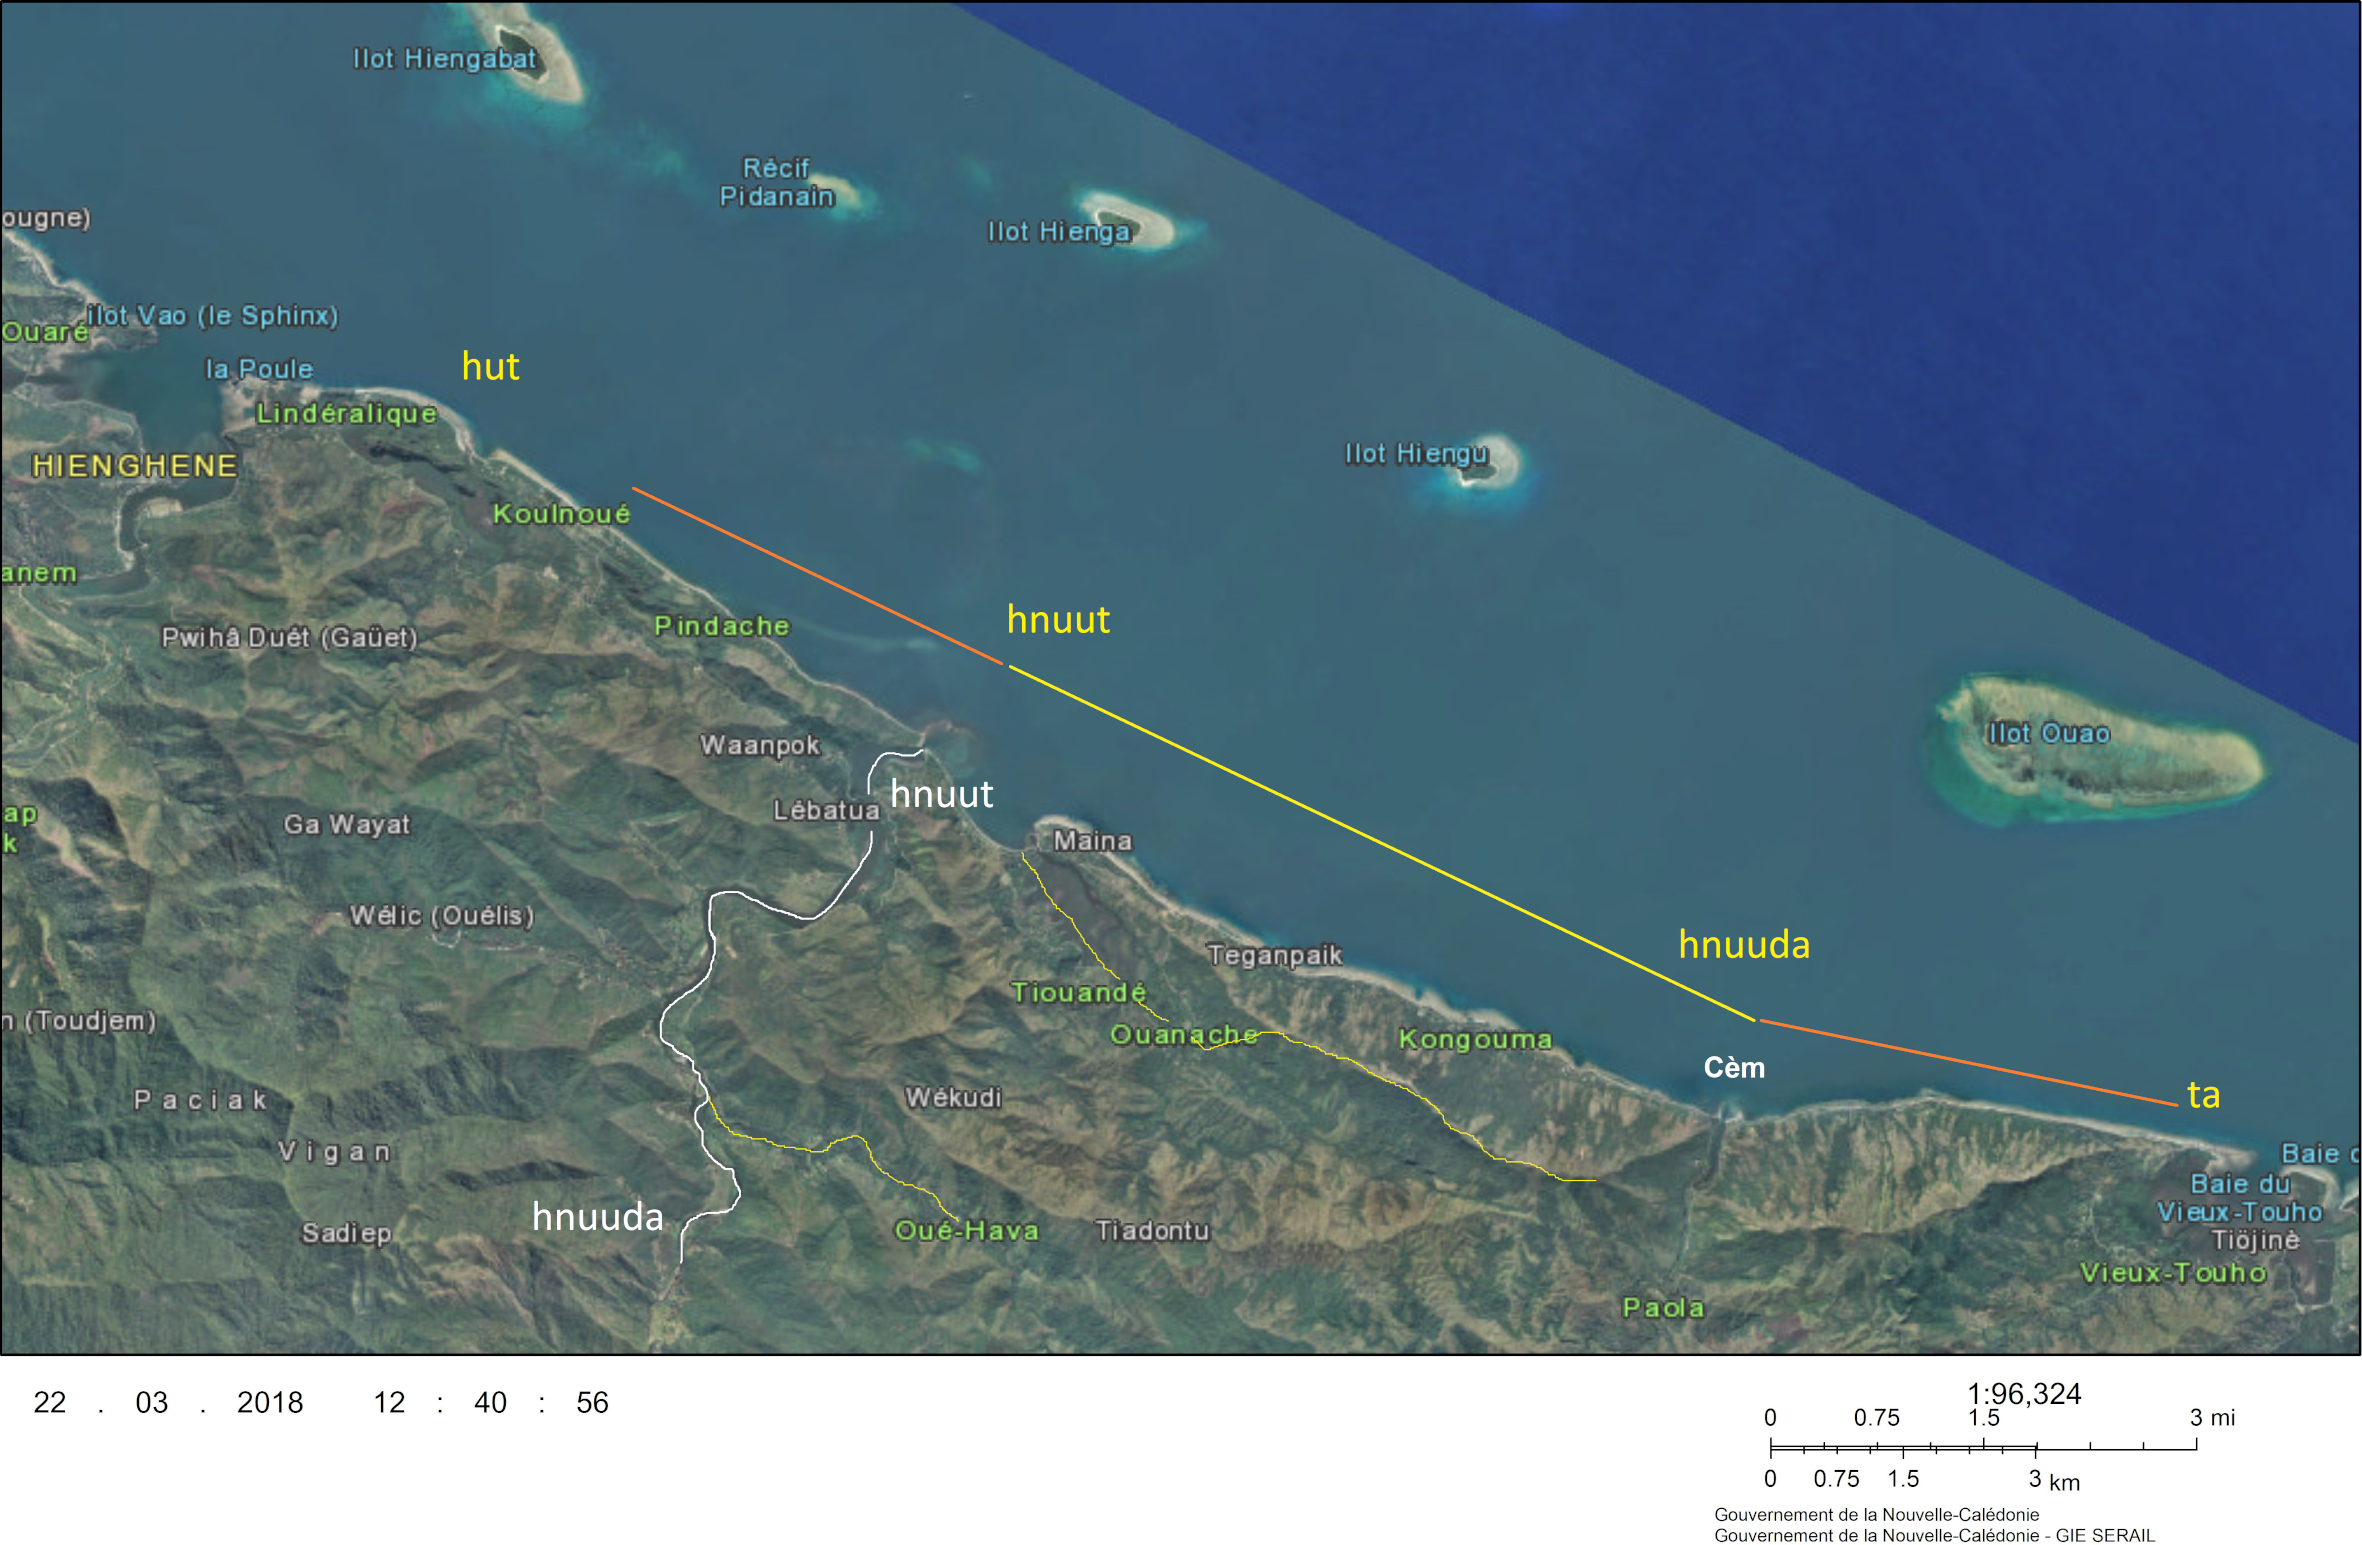
\includegraphics[width=\textwidth]{figures/map_hnuuda2.png}
	\caption{The \qu*{realm} of \textit{hnuut}. Relevant rivers marked in yellow.}
	\label{fig:map_hnuuda}
\end{figure}

\subsection{Spatial adverbs}
\label{ssec:spat_adv}
Vamale derives spatial adverbs from the verbs \textit{hut} \qu{go down}, \textit{ta} \qu{go up}, and \textit{han} \qu{move on the same level, go}. The adverbs in question, prefixed with \textit{xa-}, \textit{xa-hut} \qu{down there}, \textit{xa-da} \qu{up there}, and \textit{xa-han} \qu{over there}, form the basis of this system and are unrelated to the demonstratives in \sectref{ssec:Prox}. They are described in more detail in \sectref{ssec:prox_Adv}, but an overview is given in \Cref{tab:space}. 
Spatial words can be combined with other words (\textit{hoot xahut} \qu{far down.there}) or with each other (\textit{nyaut xahut} \qu{just down there (but too far to reach)}).

\begin{table}
	\centering
	\caption{The main motion verbs and their associated locative adverbs}
	\begin{tabular}{lll}
		\lsptoprule
		Form&Gloss&Word class\\\midrule
		\textit{cahni}& \qu{here}& adverb\\
		\textit{la}& \qu{be.here}& verb\\
		
		\textit{ta}& \qu{move up} & verb\\
		\textit{hut}& \qu{move down}& verb\\
		\textit{han}& \qu{go (same level)}& verb\\
		\textit{hnu-ut}& \qu{move downstream}&verb\\
		\textit{hnu-da}& \qu{move upstream}&verb\\
		
		\textit{xa-da}& \qu{up there}& adverb\\
		\textit{xa-hut}& \qu{down there}& adverb\\
		\textit{xa-han}& \qu{over there}& adverb\\
		\textit{xa-hnu-ut}& \qu{over there (downstream)}& adverb\\
		\textit{xa-hnu-da}& \qu{over there (upstream)}&adverb\\	
		\lspbottomrule
	\end{tabular}
	\label{tab:space}
\end{table}

 

\subsection{\textit{Nya} \qu{around, towards, inside}}
\label{ssec:nya}
\is{Space!\textit{nya} \qu{around, towards, inside}}
\textit{(H)nya} \qu{put, give, send} is a multi-purpose morpheme, especially in the context of space. One function of \textit{nya} is to combine with prepositions to form new prepositions, locating the theme as contained by or very close to the prepositioned location: \textit{ca-} \qu{at} $\rightarrow$ \textit{nye-ca-} \qu{inside} (\ref{ex:nya1}), \textit{pwa-} \qu{on top of}, $\rightarrow$ \textit{nya-pwa-} \qu{upon}, \textit{ko} \qu{on (touching a part of it)}, \textit{nya-ko} \qu{immediately on; apply on} (\ref{ex:nyako}). In this function, \textit{nya} also appears as a prefix in spatial adverbs (see \sectref{ssec:prox_Adv}), to form a proximal form (\textit{nya-ut} \qu{(put) down, down there at an arm's length}). \textit{Nya} often displays a phonologically conditioned allomorph \textit{nye} when preceding the article \textit{i} \qu{\gl{def}.\gl{sg}}, and palatal /c/, as in (\ref{ex:nya1}).


\ea\label{ex:nya1}\gll le=vwa-vaci li=apuli nye-ca i nye-ca i=mwa-n daahma\\
 3\gl{pl}=do-kernel \gl{def}.\gl{pl}=people \gl{loc}-in \gl{def}.\gl{sg} \gl{loc}-in \gl{def}.\gl{sg}=house-\gl{poss} chief\\
\glt \qu{The people were quarrelling in, in the chief's house.} {[DT:10.3]}
\z

\ea\label{ex:nyako}\gll bitake nya-ko i=yee\\
 wrap \gl{loc}-on \gl{def}.\gl{sg}=tree\\
\glt \qu{wrap around the tree} {[X9:20]}
\z

\textit{Nya} can also mean \qu{toward}, a meaning that is related to \qu{send}. In combination with spatial adverbs, \textit{nya} forms two paradigms: the series \textit{nya-xahut/nya-xada/nya-xahan} is almost equivalent in meaning to \textit{xahan} \qu{over there} etc. It means \qu{in the vicinity of X}, whereas \textit{xahan} etc. designate a more precise location.  In (\ref{ex:nya_from}) and (\ref{ex:nya_cricket}), \textit{nya} is used to express a vague area. The other paradigm combines \textit{nya-an}/\textit{nya-ut}/\textit{nya-da} \qu{send, put there/down/up} with the basic adverbial form, which yields a comparatively farther meaning, e.g. \textit{nya-an (mwa) xahan} \qu{(even) further away in this general direction} (see \sectref{ssec:spat_adv}).



\ea\label{ex:nya_from}\gll In-Fwe hapi ``In-Fwe ka e=hu-pe \textbf{nya} \textbf{nya}-da xa-da" kavi cipa a=vi i=goakan\\
 F. \gl{comp} F. \gl{cnj} 1\gl{sg}=come-\gl{dir.cp} from send-up \gl{loc}-up but \gl{neg} 3\gl{sg}=say \gl{def}.\gl{sg}=place\\
\glt \qu{Figtree-Bark said that ``[my name is] Figtree-Bark and I come from somewhere a little further up" but she didn't say the place.} {[GC:53.2]}
\z 

\ea\label{ex:nya_cricket}
\gll ka a=cuut cahni go a=cuut cai-n ka i=xa-thake i=bool. hmwakan \textbf{nya}-xahan a=cuut xahan ka i=see\\
 \gl{cnj} 3\gl{sg}=stand here \gl{cnj} 3\gl{sg}=stand behind-\gl{nspec} \gl{sbj} \gl{def}.\gl{sg}=\gl{agt}.\gl{nmlz}-throw \gl{def}.\gl{sg}=ball maybe over-there 3\gl{sg}=stand over.there \gl{sbj} \gl{def}.\gl{sg}=one\\
\glt \qu{And she stands here, and behind her stands the cricket pitcher. Maybe around there stands the other [player].} {[PJ:29]}
\z

\textit{Nya} is frequently used to locate something in a named place, especially villages, as in (\ref{ex:nya_tgnpk}). This may be a strategy to avoid having to use more specific terms such as \textit{xahut} \qu{down there}, but no clear pattern was identified.

\ea \label{ex:nya_tgnpk}\gll vwa nya theganpaik\\
 \gl{exist} around T.\\
\glt \qu{It will be in Téganpaik.} {[AG1:66]}
\z

\subsection{Same-level axis}
\is{Space!Same-level axis}
\is{Verbs!Prefixes!Manner}
Volitional displacement on the same level is expressed with the active verb \textit{han} or the derived adverb \textit{xahan} \qu{over there on the same level}. The movement of an object, e.g. in the wind, is called \textit{va(a)ya} \qu{movement, work}. Depending on the context, \textit{han} can mean \qu{go}, e.g. \textit{ha-de-ha-me} \qu{go-\gl{dir.cf}-go-\gl{dir.cp}} \qu{to and fro}, and \qu{walk}, e.g. \textit{han-maa} \qu{walk on the reef at low tide to gather sea-food}. There is an increase of the use of \textit{han} among less fluent speakers, which may be due to French influence. 

Nowadays, \textit{han} means \qu{to walk} and \textit{thêên} \qu{to run, to fly}, but the manner prefix \textit{t(h)e-} \qu{to do while walking} is probably derived from \textit{thêên}. Since this is the case for both Hienghène languages (\textit{hen} \qu{walk} in Pije, but \textit{te-} \qu{while walking}) and Voh-Koné ones, the split must be an old one.


\subsection{Centripetal/-fugal axis -\textit{me}, \textit{-le}}
\is{Space!Centripetal/-fugal}
\largerpage
There are two main suffixes used to express motion to and from the utterance's point of reference. While this center is usually the speaker, stories may set the center somewhere else more or less explicitly,\footnote{This was described for Caac as well \parencite[176]{cauchard_study_2014}.} and hypothetical or past situations can also feature these suffixes.
The movement verbs assimilate the final consonant's place of articulation to \textit{-me} \qu{\gl{dir.cp}}: \textit{ta} \qu{go up}+ \textit{-me} $\rightarrow$ \textit{tame} \qu{come up}, \textit{hut} \qu{go down} + \textit{-me} $\rightarrow$ \textit{hupe} \qu{come down}, \textit{han} \qu{go} + \textit{-me} $\rightarrow$ \textit{hame} \qu{come}. The other suffix \textit{-le} \qu{\gl{dir.cf}} assimilates to the verb's final consonant: \textit{ta-le} \qu{leave upwards}, \textit{hut-e} \qu{leave downwards}, and \textit{han-de} \qu{go away}. The latter is another example of the relationship between alveolar plosives and liquids mentioned in \sectref{ssec:ka_CL}.

Motion verbs can be added to a verb phrase if a centripetal or centrifugal meaning is needed, as other verbs cannot take \textit{-me} or \textit{-le}, as in (\ref{ex:added_hame}).
\ea \label{ex:added_hame}\gll kona sili sahmwa ha-me sili sahmwa ha-me\\ then pierce other.way go-\gl{dir.cp} pierce other.way go-\gl{dir.cp}\\
\glt \qu{Then he backs [the truck] up, backs it up.} {[KG:466]}
\z


\subsection{Origin of motion}
\label{ssec:mo_ko}
\is{Space!Origin of motion \textit{moo}}
In order to express the origin of a motion, \textit{moo} \qu{stay} is preposed to the source, and postposed to the motion verb, as in (\ref{ex:Vmoo}).

\ea \label{ex:Vmoo}\gll na tha go=saat moo cahni\\
 \gl{dem} \gl{ass} 2\gl{sg}=wade from here \\
\glt \qu{You wade in the water from here.} {[RP:6]}
\z

\subsection{Others}

This section has not made a complete description of spatial expressions in Vamale, a daunting task that has become a PhD thesis in its own right for both Nengone \parencite{bearune_lexpression_2012} and Caac \parencite{cauchard_study_2014}. The chapter mostly focused on the main axes of motion, proximity,\footnote{Proximal and distal demonstratives are discussed in \sectref{ssec:Prox}.} and centripetal/centrifugal motion, but there is a lexical field of prepositions (e.g. \textit{pwa-} \qu{on}, \textit{xala-} \qu{under}, \textit{cela-} \qu{beside}, \textit{patemwano} \qu{right next to}, \textit{ca-} \qu{at}) (see \sectref{ssec:WCPrepoNouns}), manner verbs (e.g. \textit{falogavi} \qu{move across diagonally}), and verbs describing motion more specifically, e.g. \textit{cop} \qu{go over a mountain, go to the other coast; surpass someone} or \textit{saat}\footnote{There are also \textit{sesaat} \qu{walk slowly, sneak}, and \textit{sesaaleke} \qu{stalk} which could be related.} \qu{walk through water, ford a river}. The next section leaves the lexical domain of space and addresses productive prefixes denoting posture and ways of doing things.

\section{Prefixes}
\label{sec:VPrefix}
\is{Verbs!Prefixes}
\largerpage
The following derivational prefixes are distinct from TAM markers in that they are not independent words, although they express similar meanings, and are partly sensitive to aktionsart. \Cref{tab:pref_Manner} lists them with examples.
%Many of the prefixes are derived from verbs. %todo bar
Prefixes of manner are all derived from verbs and in many cases lexicalized, though some still appear productive. \textit{The-} is a polysemous prefix, as it not only contributes its expected \qu{do while walking/running} meaning to verbs, but also takes more aspectual meanings, depending on the verb and its context (see \sectref{ssec:the}). Prefixes are presented here in \Cref{ChapterVerbs} while aspectual markers, which are own words, are described in  \Cref{ChapterAspect}, and anything that is exclusive to the verb phrase but not part of the verb, in \chapref{ChapterVP}.

\subsection{Prefixes of manner}
\label{sec:Manner}
\is{Verbs!Prefixes!Manner}
Manner prefixes can be added to roots to express how something is done, and have in many cases become lexicalized, i.e. are not added to new words, but can be identified as bearing meaning in several verbs. % %todo what is a lexicalized environment?
For example, \citeauthor{rivierre_bwatoo_2006} analyze some words as complex (e.g. \textit{tha-bilo-ke} \qu{to kill}, \citeyear[61]{rivierre_bwatoo_2006}), which are not attested without their manner prefix, or indeed with another prefix, in Vamale. Bound verbal forms which are still attested in the dictionary include: 
\begin{enumerate}
	\item \textit{-bii} \qu{crack} from POc *piti(k) \qu{crack} \parencite[276]{ross_lexicon_1998},\begin{enumerate}
		\item  \textit{cu-bi(i)} \qu{break bread} 
		\item \textit{cu-bite} \qu{be squashed by a crowd}
		\item \textit{caa-bite} \qu{harvest}
		\item \textit{ca-bi} \qu{smash something brittle by hand or blunt tool}
	\end{enumerate}
	\item \textit{-bwane} \qu{split} from POc *pʷalaq \qu{split} \parencite[265]{ross_lexicon_1998}, e.g. \textit{tha-bwane vai} \qu{split stone}, \qu{Téganpaïk (a village name)}
	\item \textit{-bali} \qu{drive in}, e.g. \textit{tha-bali} \qu{to nail}, \textit{coo-bahli} \qu{push someone away with the hand}
	\item \textit{-theeke} \qu{push}
	\begin{enumerate}
	\item \textit{pitheeke} \qu{to push someone away}
	\item \textit{caatheeke} \qu{push away with a stick}
	\item \textit{sibatheeke} \qu{push someone in a direction}
	\item \textit{tha-theeke} \qu{kill with a spear}
	\item possibly \textit{theeke} \qu{blow on food}
	\end{enumerate}
Note that in the first three examples listed for \textit{-theeke}, the preceding parts are transparent.
\end{enumerate} Manner prefixes have been described in \citetitle{ozanne-rivierre_verbal_2004}, called ``classificatory prefixes" there \parencite[349]{ozanne-rivierre_verbal_2004}, and are typical of New Caledonian languages, albeit more frequent in Southern languages than in Northern ones. It is possible that a compound consisting of a shortened transitive manner verb and an action verb was already a feature of Proto-Mainland \parencite[354]{ozanne-rivierre_verbal_2004}, as these prefixes appear throughout the main island, but have diversified clearly within the two groups North and South. Having a variety of verbs for striking with different tools is an old feature of Oceanic. \Cref{tab:POcV} (page~\pageref{tab:POcV}) gives a short selection of Proto-Oceanic verbs.\footnote{The form *sasa is given by \parencite{grace_proto-oceanic_1969}.} The posture prefixes \textit{cu-} \qu{do standing}, \textit{ta-} \qu{do sitting}, see (\ref{ex:ta-meebam}), and \textit{mi-} \qu{do lying down}, are unique to Northern languages \parencite[356]{ozanne-rivierre_verbal_2004}. Note that Ozanne-Rivierre and Rivierre call verbs prefixed by the morphemes described here ``compound verbs", whereas I use the term exclusively for verbs where all components are also attested as single head verbs.

%\textit{tha-} *sasa \qu{hunt, thrash, a whip} grace 1969xx, \textit{co-} PEO *taus(i) \qu{pluck} \parencite[279]{ross_lexicon_1998}
\begin{table}[p]
	\caption{Proto-Oceanic verbs for hitting \parencite[267]{ross_lexicon_1998}}
	\begin{tabularx}{\textwidth}{lQ}
	\lsptoprule
		 POc & Meaning\\\midrule
		 *sasa &\qu{hunt, thrash, a whip}\\
		  *punu(q), *punuq-i-& \qu{hit, strike, fight, kill}\\
		  *qubu, *qubWi-& \qu{hit with fist or with a weapon}\\
		  *rapu(t), *raput-i- & \qu{hit with hand or stick, slash}\\
		  *tutuk, *tuki[-]& \qu{pound, mash by pounding, hammer, crack by hammering}\\
		  *putu(k) and *butu(k), *butuk-i-& \qu{repeatedly knock,  pound, beat}\\
		  *qatu(1), *qatu-J-i- & \qu{strike from above, pound}\\
		  *babak, *baki[-]  & \qu{strike one against another, knock}\\
		  *tupu, *tupu-i-& \qu{knock against, knock over, stub (toe), stumble against}\\
		  *pwasa(r,R), *pwasa(r,R)-i­& \qu{slap, hit}\\
	  \lspbottomrule
	\end{tabularx}
\label{tab:POcV}
\end{table}
 
\begin{table}[p]
	\caption{Manner prefixes, their likely origins, with examples.}
	\small
	\fittable{%
	\begin{tabular}{lllll}
		\lsptoprule
		Form & Meaning & Origin & Example & Meaning\\
		\midrule
		\textit{ca-} & hit with hand & & \textit{cabi} & \qu{smash something brittle}\\
		\textit{caa-}& set down foot& \textit{caa}&\textit{caa-gati} & \qu{crush something soft}  \\
		&&&\textit{caa-thiho} & \qu{limp}\\
		\textit{co}- & with hand & &\textit{co-gavi} &\qu{break by pulling} \\
		&&&	\textit{co-bahli}&\qu{push off by hand}\\
		\textit{ta}- & sitting & \textit{tabo} & \textit{ta-meebam} & \qu{sit-sleep; sleep in a sitting position}\\
		\textit{cu-} & standing & \textit{cuut}& \textit{cu-vathan-ke} & \qu{stand-each-\gl{tr}; stand apart from e. o.}\\
		\textit{mi-} & lying & \textit{majit}&  \textit{mi-xaleke} & \qu{lay-see; have a vision}\\
		\textit{tha-} & forcefully & \textit{thake} & \textit{tha-biloke} & \qu{strongly-kill; kill with a strike}\\
		&&&\textit{tha-gavi}&\qu{strongly-cut; cut with one strike}\\
		\textit{so-} & touch & \textit{soot} & \textit{so-teet} & \qu{touch-lazy; do carelessly}\\
		\textit{fa-}%\footnotemark
		& speak& \textit{fati} & \textit{fa-xhopwen} & \qu{talk big, boast}\\
		\textit{t(h)e-} & do walking & \textit{thêên} & \textit{t(h)e-thagavi} &\qu{walk-cut; take a short-cut}\\ 
		\lspbottomrule
	\end{tabular}}
\label{tab:pref_Manner}
\end{table}
%\footnotetext{\textit{fa-vamale} \qu{speak Vamale} seems to be a de-nominal derivation, whereas the other prefixes attach onto verbs.}

\ea \label{ex:ta-meebam}
\gll bo tha xa-vaaya-n-eo i=  m=e=ta-meebam aa ca-n sohmun\\
 \gl{irr} \gl{ass} \gl{agt}.\gl{nmlz}-work-\gl{poss}-1\gl{sg}.\gl{poss} \gl{def}.\gl{sg} \gl{subr}=1\gl{sg}=sit-sleep uuh in-\gl{nspec} study\\
\glt \qu{That would be my habit, the\ldots if I slept sitting in school.} {[2017-10-30 Pauty Ecole et punition:10]}
\z

\subsection{\textit{the-} }
\label{ssec:the}
\is{Verbs!Prefixes!\textit{the-} \qu{quickly, a bit; while walking}}
The prefix \textit{the-} is halfway between a prefix of manner and an aspect marker. It likely comes from \textit{thêên} \qu{run, fly} and still exists as a manner prefix, as illustrated in the words \textit{the-thagavi} \qu{take a shortcut} and \textit{the-yathô} \qu{walk-stress; walk in a hurry}. It seems, however, that this use has become lexicalized.
%\ex
%\label{ex:the_manner}
%
%\ili{}{}{} Jean-Philippe, 11.7.2019, p.20
%\gll the-th
%
%
%
%\glt
%
%
%\z

The productive, non-manner prefix \textit{t(h)e-} has two meanings, depending on the aktionsart of the verb. With punctual verbs, it means \qu{do quickly, a bit}. With durative ones, it means \qu{do continually since earlier}, often with reference to another event, e.g. \textit{the-xaleke} \qu{look at constantly}, and (\ref{ex:constant_the}). This is likely due to its putative origin \textit{thêên} \qu{run, fly}. In imperatives, \textit{the-} always asks for immediate action: \qu{do this now}. 
While \textit{the-}prefixed verbs, when preceded by TAM markers, often do not take on idiosyncratic meanings, some combinations are interesting. Frequentative \textit{mu}, habitual \textit{xa}, and imperfective/future \textit{bwa} do not change the meaning, but \textit{pa} \qu{\gl{prf}} excludes an interpretation of the event as quickly done; the yielded meaning focuses on the time spent on it (``it took me a long time to do it"). This effect is even stronger with \textit{pa ja} \qu{\gl{prf}.\gl{prf}}. With progressive \textit{kon}, \textit{the-} means \qu{right now, immediately}. 
With durative verbs, \textit{the-} takes on a durative, imperfective meaning, and is similar in function to the adverb \textit{hnyana} \qu{constantly}.\footnote{See \textit{hnyana-} \qu{breath}, from which it is probably derived.} Compare the pair of examples (\ref{ex:constant_hnyana}) and (\ref{ex:constant_the}) for said similar meanings, but see examples (\ref{ex:the_vs_hnyana}) and (\ref{ex:the_vs_hnyana2}) for the differences.


\ea\label{ex:constant_hnyana} \gll ceme o vaya tha xalo ko-n tele hnyana\\
 \gl{subr}.1\gl{sg} \gl{irr} work \gl{ass} gaze \gl{obl}-\gl{nspec} TV constantly\\
\glt \qu{Whenever/If ever I work, he'll watch TV (while and as long as I work). [Jean-Philippe, 11.7.2019, p.20]} {}
\z 

\ea\label{ex:constant_the}
\gll ceme o vaya tha the-xalo kon tele\\
 \gl{subr}.1\gl{sg} \gl{irr} work \gl{ass} \gl{thedur}-gaze \gl{obl}-\gl{nspec} TV\\
\glt \qu{Whenever/If ever I work, he'll watch TV (while and as long as I work).}
\z

\begin{sloppypar}
When describing a situation that is unique and limited in time, \textit{the-} and \textit{hnyana} are interchangeable. However, more general, or abstract, situations, \textit{the-} \qu{\gl{thedur}} takes a meaning similar to \textit{the-} \qu{\textsc{the\textsubscript{punct}}}, see examples (\ref{ex:the_vs_hnyana}) and (\ref{ex:the_vs_hnyana2}). This is reminiscent of \textit{mwa} \qu{again, now, however} in \sectref{sec:WCRepetitive}.
\end{sloppypar}

	\ea \label{ex:the_vs_hnyana}
	\gll tha go=the-xaleke\\
		 \gl{ass} 2\gl{sg}=\gl{thedur}-see\\
	\glt \qu{You see now.}
	\z 
		
	\ea \label{ex:the_vs_hnyana2}
		\gll tha go=xaleke hnyana\\
	 \gl{ass} 2\gl{sg}=see constantly\\
	\glt \qu{You often see.}
		\z


%\subction{Imperative use of \textit{the-}, and \textit{xhaa-}}
\is{Clauses!Imperative clauses}

\textit{The-} can be used with imperative verbs, where it asks for immediate action: \qu{do this now, do this quickly}. Another prefix, \textit{xhaa-} \qu{\gl{att}}, only appears in the imperative mood and acts as an attenuative prefix, \qu{do a bit} (\ref{ex:the_imp}). In some scenarios, the two have similar meanings.% shortens vowel if combined with e.g. \textit{da}, \textit{the}, etc. possibly not phonemically long vowel.

\ea \label{ex:the_imp}\gll xhaa-thagavi ye-mwago ma go=xaleke i=vaaya koo-n\\
 \gl{att}-cut tree-mango \gl{subr} 2\gl{sg}=see \gl{def}.\gl{sg}=work \gl{obl}-\gl{nspec}\\
\glt \qu{Just (try to) cut a mango tree and you’ll see the work it is.} {[example sentence provided for the dictionary entry on \textit{xhaa}]}
\z
 
The attenuative meaning of \textit{xhaa-} is found with imperative \textit{the-} when the latter is used to suggest that the action asked for will be quick. The difference, however, is that \textit{the}- suggests a quickly done task, whereas \textit{xhaa}- means you do something for a short while, without necessarily finishing what you started. \textit{The-} and \textit{xha(a)-} can be combined (\ref{ex:xhaa}). When combined, their meaning depends on the verb's aktionsart: \qu{quickly do now (\gl{punc})}, \qu{do a non-committally big or small bit of it (\gl{dur})}.

\ea \label{ex:xhaa}
\gll xhaa-the-thagavi cahni\\
 \gl{att}-\textsc{the\textsubscript{punct}}-cut here\\
\glt \qu{Just cut it here real quick.}
\z

\subsection{\textit{da} \qu{do first}, \textit{ra-} \qu{do afterwards}}
\is{Verbs!Prefixes!\textit{da} \qu{do first}}
Two morphemes can be used to sort an action with respect to other actions: \textit{da(a)} \qu{do first} (\ref{ex:da_first}), and \textit{ra-} \qu{do afterwards} (\ref{ex:ra}). Note that the latter is the only phonemic example of /ɾ/, and was only encountered in elicitation sessions. A similar \textit{ra-} \qu{continue to (while others have stopped)} in Bwatoo is perhaps cognate \parencite[56]{rivierre_bwatoo_2006}.


\ea\label{ex:da_first}\gll da bale ca i=xhoogo-n-go, ka go=bo vwa thuan nya pala li=been\\
 do.first broom in \gl{def}.\gl{sg}=home-\gl{poss}-2\gl{sg}.\gl{poss} \gl{cnj} 2\gl{sg}=\gl{irr} do do.well in home \gl{def}.\gl{pl}=peer\\
\glt \qu{First clean up your home, then you (may) go clean up other homes.} {[Proverb]}
\z 


\ea\label{ex:ra}\gll go=bo ra-ha-me\\
 2\gl{sg}=\gl{irr} later-go-\gl{dir.cp}\\
\glt \qu{You'll come afterwards.} {[21.07.2019 p.42]}
\z
%Suffix "do in advance, go ahead"

\textit{da} \qu{to do first, in advance} is more common than \textit{ra-}, and contrary to the latter, can take stress (\ref{ex:da1}). It does not head phrases, however. It will hence be analyzed as a pre-verb.


\ea\label{ex:da1}
[e ˈⁿdaː viː ɲãkɔ̃ːm]\\
\gll e=da vii nyakoo-m\\
 1\gl{sg}=in.advance tell \gl{obl}-2\gl{sg}\\
\glt \qu{I am warning you.} {[D3:79]}
\z


\ea
\gll  gase=da xhwi-aman kon gase=bwa vwa \textit{coutume}\\
 1\gl{pl}.\gl{incl}=in.advance eat-thing then 1\gl{pl}.\gl{incl}=\gl{ipfv} do custom\\
\glt \qu{We'll eat first, then we'll conduct the ceremony.} {[L1:31]}
\z

%\ea
%\ea
%
%\gll han-da
% go-ahead
%\glt \qu{go ahead}
%
%\ea
%
%\gll vwa-ta 
% do-advance
%\glt \qu{do in advance}
%
%\z

\subsection{Pluractional \textit{e-}}
\label{ssec:pluriactional}
\is{Pluractional \textit{e-}}
\is{Verbs!Prefixes!Pluri-actional}
A pluractional prefix \textit{e-} occurs in various constructions where several entities perform the same action at the same time, but not to each other, e.g. (\ref{ex:ehan_caile}) and (\ref{ex:etipwa}). The prefix is reconstructed to be a reflex of POc *paRi-, which otherwise has reflexive, reciprocal, and middle functions. If \textit{e-} were left out, the pluractional meaning would be lost, and the participants would be engaged in their activities in a more individual manner: compare examples (\ref{ex:ehan_cain}) and (\ref{ex:ehan_caile}) to \textit{le han cai-n} \qu{They follow him} and \textit{le han cai-le} \qu{They follow them}. Note that in constructions such as (\ref{ex:ehan_caile}), the meaning is somewhat in between reciprocal (they follow each other), further described in \sectref{sec:refl}, and pluractional (they each follow a different person). This is called ``chaining" by Bril, and widely attested throughout the archipelago \parencite[32, 47]{bril_semantic_2005b}.
%Why is this MID? Can the same predicate occur without e-? Or is it a medium tantum? Or is it just the plurality of referents that triggers/favors (?) the MID marking?

\ea\label{ex:ehan_cain}\gll le=e-han cai-n\\
 3\gl{pl}=\gl{mid}-go behind-3\gl{sg}\\
\glt \qu{They \textit{all} follow him/her.} {[07.11.18 p.93]}
\z


\ea\label{ex:ehan_caile}
%This is not really reciprocal is it? It seems more like a "all do this"\gll le=e-han cai-le\\
 3\gl{pl}=\gl{mid}-go behind-3\gl{pl}\\
\glt \qu{They walk one after the other (single file).} {[07.11.18 p.93]}
\z


\ea\label{ex:etipwa}\gll le=e-tipwa pu ka li=xhaapwe sep\\
 3\gl{pl}=\gl{mid}-fall be.on.the.ground \gl{sbj} \gl{def}.\gl{pl}=fruit coco\\
\glt \qu{The coconuts fell all together.}\\\relax
[vamale-181107-jpnelemwa-04: 00:01:19-00:01:24]
\z
 

\ea\label{ex:tipwa_hato}\gll le=tipwa hut hato ka li=xhaapwe sep\\
 3\gl{pl}=fall go.down do.alone \gl{sbj} \gl{def}.\gl{pl}=fruit coco\\
\glt \qu{The coconuts fell by themselves (without known cause).} {[vamale-181107.jpnelemwa-04: 00:00:30- 00:00:32]}
\z

A difference between reference and occurrence, i.e. whether several things happen at once, or the same action several times, is made analytically, by adding \textit{sisipo} \qu{together} at the end of the verb phrase, or \textit{vataan} \qu{each, individually} as a preverb. 

In (\ref{ex:ve-moo}), similarly to contexts of \textit{mee} \qu{all} described in \sectref{ssec:se-me}, the action is performed by several people together. However, while \textit{mee} usually merely implies that out of a group, everyone participates, \textit{(v)e-} here adds a semantic trait of indistinguishability \parencite[66--73]{kemmer_middle_1993}. The participants sit together and form an indistinct group, whose members do not participate in the sitting separately.

%\todo{How can the agents be affected by staying and going down? You would have to show a contrast and actually test for affectedness...}
%xx

\ea \label{ex:ve-moo}
%\ili{}{}{} 
\gll go tha le=ve-moo mwa moo mwa \\
 well \gl{ass} 3\gl{pl}=\gl{mid}-stay \gl{rep} stay \gl{rep}\\
\glt \qu{Well and then they all stay together, stay.} {[KL:220]}
\z


\ea
%\ili{}{}{
\gll th=abe xa-e-hut ca-n jigo\\
 \gl{ass}=1\gl{pl}.\gl{excl} \gl{nmlz}.\gl{agt}-\gl{mid}-go.down in-\gl{nspec} mangrove\\
\glt \qu{We all used to go down to the mangrove (to play).} {[PE1:107 ]}
\z


\section{Complex verbs}
\label{sec:ComplexV}
\is{Verbs!Complex verbs}
This section introduces three ways in which Vamale forms complex verbs. Following an ancient Oceanic tradition, some verbs are reduplicated. Though not very prevalent in Vamale, some examples are discussed in \sectref{sec:redup}. Verbs and other verbs may join to form compounds, and verbs and nouns are also frequent partners in the creation of new words. 

\subsection{Reduplication}
\label{sec:redup}
\is{Reduplication}
\is{Verbs!Reduplication}
True reduplication in Vamale is rare. Cases abound where a verb is repeated, to express the length, urgency, intensity etc. of a notion: most frequent is the context of a serial verb construction (described in \sectref{sec:SVC}), but verbs are also repeated in a poetic context such as in (\ref{ex:xho}), or in a playful one (\ref{ex:javelo}). These verbs usually have their own prosodic environment and the whole construction is lexically transparent.\largerpage[-1]


\ea \label{ex:xho}
(Cicada-hunting children's song)\\
\gll tabo tabo li=xho thamo thêên thêên li=xho xayu\\
 sit sit \gl{def}.\gl{pl}=cicada female fly fly \gl{def}.\gl{pl}=cicada male\\
\glt \qu{Sit sit oh female cicadas [full of eggs], fly fly (away) oh male cicadas.} {[vamale-181121-xho\_thamo]}
\z

\ea \label{ex:javelo}
(Stone-skipping call)\\
\gll jaaaavelo-velo-velo-velo\\
 ricochet\\
\glt \qu{ricochet-chet-chet-chet}
\z

The attested cases in which a word is repeated and forms a new word are the following: \textit{fwa-fwa} \qu{hole-hole} \qu{full of holes}, \textit{vaya-vaya} \qu{move-move} \qu{wobbly}, and \textit{xhasaat-xhasaat} \qu{jump-jump} \qu{hobble, jump around on one foot or to get warm}. While the consultant said that there were many other cases, I found none.

\subsection{Compound verbs}
\label{ssec:CompoundV}
\is{Verbs!Compound verbs}
\largerpage[-2]
Compound verbs are composed of a verb, which determines the resulting construction's word-class and often plays a dominant role in its semantics, and another element. The interesting case of the verb \textit{hnya} \qu{put, send} and spatial adverbs such as \textit{xahan} \qu{over there}, which combine to \textit{(h)nya-xahan} \qu{in this direction}, is an exception. These combined words are adverbs (see \sectref{ssec:nya}), as evidenced by verb phrases like \textit{hnya hnya-xada} \qu{put over there}, and will not be discussed further here.

An important group of compound verbs are composed of the vague verb \textit{vwa} \qu{do}, and a specifying verb, e.g. \textit{vwa-suu} \qu{do break} \qu{pay someone}, \textit{vwa tau} \qu{do impact} \qu{fish},\footnote{This is almost certainly a taboo avoidance strategy. Hunters never use \textit{vap} \qu{to hunt} if they go out, instead they say \textit{balan thaap} \qu{length nyaouli [a savannah tree species]} when describing their plans, to avoid bad luck. \textit{Vwa tau} would have replaced the marked word. Word avoidance taboos are commonplace in this region of the world. Perhaps the word for \qu{wound}, \textit{ape aman} \qu{trace\slash track of something} is kept vague on purpose.\is{Word avoidance taboo}} or \textit{vwa-thiho} \qu{do-stumble} \qu{do by accident}. Another group, small but very often used, are the lexicalized serial verb constructions (SVCs) with \textit{fe} \qu{take} and motion verbs, e.g. (\ref{ex:feame}). Other verb compounds also seem to be lexicalized SVCs, e.g. \textit{saahma-cuut} \qu{rise-be.standing} \qu{to stand up}, and \textit{ha-de-ha-me} \qu{go-\gl{dir.cf}-go-\gl{dir.cp}} \qu{move to and fro}.

\ea \label{ex:feame}
\gll fe-(h)a(n)-me\\
 take-go-\gl{dir.cp}\\
\glt \qu{bring}
\z 

\subsection{Incorporated object constructions}
\label{ssec:CompV}
\is{Verbs!Incorporated object construction}
\begin{sloppypar}
On top of combining verbs with other verbs, Vamale also forms grammatical words from verbs and non-specific arguments: this includes everyday activities incorporating the most common undergoer, e.g. \textit{xhajake-lait} \qu{eat.starchy-rice} \qu{eat rice}, \textit{xhwi-aman} \qu{eat.proteiny-something} \qu{eat something}, \textit{vai-xam} \qu{weave mats}. This is called ``incorporated object construction" by \citet[357]{ozanne-rivierre_verbal_2004}. There are numerous verbs formed with \textit{vwa} \qu{do}, e.g. \textit{vwa-vaci} \qu{do-pit, hard part}  \qu{to argue}, \textit{vwa-ikin} \qu{do-meaty.side-dish} \qu{to eat tubers with meat}, \textit{vwa-khêt} \qu{do-quarz, blade} \qu{to shave}. All the verbs mentioned form a single stress-contour and cannot be split without losing their overall meaning.
Some nominalized forms can contain complex verbs including a noun, such as \textit{xa-thêên-fe-\textbf{fati}} \qu{\gl{agt}.\gl{nmlz}-run-take-word} \qu{messenger} and \textit{xa-fe-ta-me-\textbf{mapeke}} \qu{\gl{agt}.\gl{nmlz}-take-go.up-\gl{dir.cp}-bright} \qu{morning star}. 
\end{sloppypar}

\section{Nominal derivation}
\label{sec:NomDeriv}
\is{Verbs!Nominalization}
\is{Nominalization}

Vamale derives nouns from verbs either by using nominalizing prefixes or simply by stripping the verb from its subject indices (be they proclitics or suffixes), and preposing an article. The nominalizers (e.g. \textit{e-, xa, hun-}) are analyzed here as prefixes because they directly attach to the root, the article, e.g. \textit{i=} \qu{\gl{def}.\gl{sg}} can only occur before it (\textit{i=xa-xaleke, *xa=i=xaleke}). 
%``Derivation" means that one only needs a subject marker on the stem to make it a verb, but you don't, instead you put a nominalizer, and you have a noun.xx
The resulting nominalized construction can be used as an argument with a verb or a preposition and can be possessed by another nominal phrase. The possessor is not, however, understood to be the agent of the action, as in English (e.g. \qu{my seeing the brother}), except for intransitive verbs. Instead, the possessor denotes the undergoer. %%todo sondern wie wird es verstanden, oder wo sagst du mehr darüber?
%What makes them nominal is the slot. \textit{i=} can attach to it, adjectives can, it can function as an argument to a verb (whereas a verb cannot have a verb as an argument I think).xx
Whether a given verb is nominalized via prefixation or stripping is lexically determined, since nominalizing via stripping is not accepted for some verbs (e.g. \textit{*i thapoke} \qu{the beginning}, or \textit{*i hmanan} \qu{his/her hunger}). Another example is \textit{hun-vwa kan} \qu{manner-do it; the style of doing it, the act of doing it} which cannot be \textit{*vwa kan} or even \textit{*vwa}. Both stripped and prefixed nominalizations may include arguments, as in (\ref{ex:i_jili}), but not TAM markers. 
Stripped nominalizations, contrary to the other de-verbal constructions detailed below, do not express a subject through possessive means, but keep the same strategy as normal verb phrases, i.e. using a noun phrase flagged with \textit{ka} \qu{sbj}: \textit{ka li=apuli} \qu{\gl{sbj} \gl{def}.\gl{pl}=person} in (\ref{ex:i_jili}). There are two relatively neutral prefixes, \textit{ape-X} meaning \qu{fact of doing X}, and \textit{hun-} \qu{manner of doing X}, though \textit{hun-} was the only one readily used by speakers for novel constructions. 

%
%\begin{enumerate}
%	\item We have \textbf{canonical nouns}, alienably or inalienably possessed.They alone do not constitute a clause. (*\textit{i daahma.}).
%	\begin{enumerate}
%		\item We have verbs that are nominalized with an obligatory  \textsc{nmlz} prefix when preceded by an article: \textit{i ape-hnyimake-aman} \qu{the fact-think-something; the thought} %(tentatively called "the NOM-needers").
%		\begin{itemize}
%			\item \textit{thapoke} \qu{begin}, ambitransitive, must be \textit{ape-thapoke-ka-n} (place-begin-acc-inan) \qu{the moment of beginning} or \textit{hun-thapoke-o/go/a/...} (manner-begin-1\gl{sg}...) \qu{the a{}ct of beginning} (this pattern is the same for all similarly nominalized verbs).
%			\item \textit{vii} \qu{say}, transitive, must carry the prefix \textit{hun-}.
%			\item \textit{moo} \qu{stay} \textbf{intransitive} must be \textit{hun-moo}.
%		\end{itemize}
%		\item We have nominalizations of entire verb phrases. This is still productive and probably an old construction.  like \textit{jili} \qu{build with wood}. They keep their object NPs in the VP. %No possession of objects like in English \textit{the speaking \textbf{of} the word}. 
%		No possession of the resulting construction attested. What works is a complete clause with a \textit{ka} subject nominalized with an article, as shown in \ref{ex:i_jili}. 
%	\end{enumerate}
%\end{enumerate}  

	\ea
	\label{ex:i_jili}
	\gll e=xaleke i=jili i=bwaakala ka li=apuli\textsubscript{\gl{sbj}}\\
	 1\gl{sg}=see \gl{art}.\gl{sg}=build.with.wood \gl{art}.\gl{sg}=pirogue \gl{sbj} \gl{art}.\gl{pl}=people\\	
	\glt \qu{I see the building of the pirogue by the men.}
		\z



\subsection{\textit{e}-}
\label{ssec:ins.nmlz}
\is{Nominalization!Instrumental nominalizer}
The instrumental nominalizer \textit{e-} has \textit{fe-} and \textit{ve-} cognates in related Northern languages. It is likely that \textit{v-} was only recently dropped, as the word for \qu{spoon} was only coined in the last 150 years, and is \textit{vetupi} from \textit{tuuvi} \qu{scoop up from liquid} (though a loan from a more archaic dialect is not excluded). The word for \qu{learning} \textit{eca} is still listed as \textit{veca} by Leenhardt (1946) and pronounced that way by Chief Luc. In Nelêmwa, a similar morpheme \textit{-ve-} or \textit{-vi-} depending on animacy \parencite[194]{bril_complex_2004}, comes from \textit{fhe} \qu{take} in Nêlêmwa (\textit{fe} in Vamale), though it is not a nominalizer (\textit{baa-}, \citealt[74]{bril_nelemwa_2002}). Our nominalizer \textit{e-} might have a similar background to Nelêmwa \textit{-ve-}, being derived from \textit{fe} \qu{to take}. Cèmuhî and Paicî use \textit{be-} \qu{\gl{ins}.\gl{nmlz}} \parencites[257]{rivierre_langue_1980}[42]{rivierre_dictionnaire_1983}, versus the reciprocal/middle \textit{pi-} \parencites[257]{rivierre_langue_1980}[363]{rivierre_dictionnaire_1983}.

\begin{enumerate}
	\item \textit{e-vwa-tiike} \qu{pen} (lit. \qu{\gl{ins}.\gl{nmlz}-make-write})
	\item \textit{e-xadae-ke} \qu{blessing} (lit. \qu{\gl{ins}.\gl{nmlz}-up.there-\gl{tr}})
	\item \textit{e-vwadi-ya-n} \qu{thumb} (lit. \qu{\gl{ins}.\gl{nmlz}-peel-starchy.food-3\gl{sg}.\gl{poss}})
	\item \textit{e-xhwali-aman} \qu{fork} (lit. \qu{\gl{ins}.\gl{nmlz}-stab-thing})
	\item \textit{e-ja} \qu{scales} (lit. \qu{\gl{ins}.\gl{nmlz}-measure, weigh})
\end{enumerate}

Other items look like nominalizations, but the meaning of the presumed base form is lost: \textit{e-xhaat} \qu{paddle}, \textit{e-thadala} \qu{fruit-picking rod}. 

\subsection{\textit{xa}-}
\label{ssec:agt.nmlz}
\is{Nominalization!Agentive nominalizer}
\textit{Xa-} \qu{\gl{agt}.\gl{nmlz}}, an agentive nominalizer, is probably derived from \textit{xayu} \qu{male}. Since in Vamale, modifiers usually follow the modified, and possessors the possessum, \textit{xa-} may be an old phrase head, now incorporated into the former modifying phrase. The nominalizer may have developed from a noun phrase with an optionally marked relative clause (\ref{ex:xavwatau}), which was gradually reduced to \textit{xay(u) vwa-tau}, and finally to \textit{xa-vwa-tau} \qu{fisherman}.

	\ea \label{ex:xavwatau}
		\gll xayu (a=a=) vwa-tau\\
	 male (\gl{rel}=3\gl{sg}) make-impact\\
	\glt \qu{the man who fishes} (the relativizer \textit{a} is often omitted)
		\z

The morpheme means \qu{one who does regularly, one whose job is X}, the former meaning being used with a habitual meaning on verbs. It can also attach to stative verbs like \textit{xahnang}, but in this case it is a habitual marker (and not a nominalizer), since the verbs can still take subject index marking: \textit{xa-xahnang-go} \qu{you are beautiful, you are a good person}. %See \textit{xada} \qu{your turn} and \sectref{sec:RecipRelations}.

\begin{itemize}
	\item \textit{xa-vabun} \qu{thief}
	\item \textit{xa-moo xada Wanaa} \qu{an inhabitant of Wanaa}
	\item	\textit{xa-vap} \qu{hunter}
	\item	\textit{xa-vwa suki} \qu{buyer}
	\item	\textit{xa-fe-ta-me-mapeke} \qu{morning star, light-bringer (lit. \gl{agt}.\gl{nmlz}-take-go.up-\gl{dir.cp}-be.bright)}
\end{itemize}

%Alsoː \textit{xa-da} \textit{xa-hut} \textit{xalan} \qu{under} yo emoo xalan thu, yo emoo Koné. NP?

The habitual meaning can be extended to express whether something has occurred in general, as in (\ref{ex:xa}).

\ea \label{ex:xa}
%\ili{}{}{} 
\gll go=pa xa-ha-me\\
 2\gl{sg}=\gl{prf} \gl{agt}.\gl{nmlz}-go-\gl{dir.cp}\\
\glt \qu{You've been here before (lit. you're already a comer).} {[21.07.2019 p.42]}
\z


A prefix \textit{xa-} is also used in reciprocal kinship terms. They are listed in \Cref{tab:recp_rel1}, and will be mentioned again in \Cref{tab:recp_rel}. For many terms, an (re-)anal\-y\-sis of \textit{xa-} as the agentive prefix makes sense, but cognates in other Northern languages suggest a different origin. Note that \textit{mwaa-n} probably actually means \qu{child-in-law of the opposite sex}. By analogy, \qu{father-in-law and his daughter-in-law} may have been \textit{xa-mwaa-n xayu}, though this word is lost nowadays.

\begin{table}
\caption{Reciprocal kinship terms}
\begin{tabularx}{\textwidth}{lQQ}
	\lsptoprule
	Complex form & Gloss of Morphemes & Meaning\\
	\midrule
	\textit{xa-bate}& \textit{xa}-tip & \qu{brothers}\\ 
	\textit{xa-betha} & &\qu{sisters}\\ 
	\textit{xaa-vap-an} &\textit{xa}-hunt?-\gl{poss}& \qu{siblings}\\ 
	\textit{xa-fa-thau-n} & \textit{xa}-\gl{caus}-wealth-\gl{poss} &\qu{brother-in-law and sister-in-law}\\ 
	\textit{xa-nya-pwan-an}& \textit{xa}-put-on-\gl{poss} & \qu{paternal aunts}\\ 
	\textit{xa-e-vwona-n}& \textit{xa}-\gl{recp}-maternal.uncle-\gl{poss}& \qu{maternal uncle and niece/nephew}\\ 
	\textit{xa-vabu-n} &\textit{xa}-grandchild-\gl{poss}& \qu{grandfather and grandchildren}\\	
	\textit{xaa-maci}& \textit{xa}-? & \qu{father and child}\\	
	\textit{xa-e-bee-n}&\textit{xa}-\gl{recp}-brother, cousin, peer-\gl{poss}& \qu{cousins}\\			
	\textit{xa-ive-n} &\textit{xa}-sister.in.law-\gl{poss}& \qu{sisters-in-law}\\			
	\textit{xa-xayaa-n}&\textit{xa}-\qu{stranger, guest}-\gl{poss}& \qu{husband and his brother-in-law}\\
	\textit{xa-mwaa-n thamo}&\textit{xa}-daughter-in-law-\gl{poss} woman& \qu{mother-in-law and her son-in-law}\\
	\lspbottomrule
\end{tabularx}
\label{tab:recp_rel1}
\end{table}
     
\subsection{\textit{hun}-}
\label{ssec:hun}
\is{Nominalization!Manner nominalizer}
This nominalizer expresses a manner of doing something. Cognates are \textit{u-} in Nelêmwa and \textit{kae-} or \textit{hun-} in Pije \parencite[253]{haudricourt_dictionnaire_1982}. No etymology is reconstructed yet for either. It often associates with the linker \textit{ka-n} \qu{\gl{link}-\gl{nspec}}. For a description of \textit{-ka-n} \qu{-\gl{link}-\gl{nspec}} see \sectref{kan}.

\begin{itemize}
	\item \textit{hun-moo ka-n} \qu{\gl{nmlz}-be \gl{link}-\gl{nspec}} \qu{way of life, nature}
	\item \textit{hun-tiike ka-n} \qu{\gl{nmlz}-write \gl{link}-\gl{nspec}} \qu{orthography}
	\item \textit{hun-thêên ka-n} \qu{\gl{nmlz}-run \gl{link}-\gl{nspec}} \qu{driving style}
\end{itemize}

As with other derivations, whether \textit{hun-} means \qu{style} or \qu{tradition}, or something more idiosyncratic, can depend on the verb. Compare examples (\ref{ex:hun}--\ref{ex:hunvi1}): \textit{moo} \qu{to stay} keeps the same meaning for inanimate and animate subjects (\ref{ex:hun1}, \ref{ex:hunmoo}). However, the derivation of \textit{vii} \qu{to say} takes on an idiosyncratic meaning with inanimate subjects, \qu{its meaning} (\ref{ex:hunvi2}) and it keeps a transparent one with an animate subject: \qu{his/her way of saying} (\ref{ex:hunvi1}).


\ea \label{ex:hun}
\label{ex:hun1}
	\gll hun-moo ka-n\\
	 \gl{nmlz}-be \gl{link}-\gl{nspec}\\
	\glt \qu{its nature}
	\z
	
	
	\ea\label{ex:hunmoo}
	\gll hun-moo-a\\
	 \gl{nmlz}-stay-3\gl{sg}\\
	\glt \qu{her/his character}
	\z
	
	\ea\label{ex:hunvi2}
	\gll hun-vii ka-n \\
	 \gl{nmlz}-say \gl{link}-\gl{nspec}\\
	\glt \qu{(its) meaning}
\z
\ea\label{ex:hunvi1}
	\gll hun-vii-a\\
	 \gl{nmlz}-say-3\gl{sg}\\
	\glt \qu{his/her way of saying it}
	\z
 
Compared to the other nominalizing prefixes, \textit{hun-} is the most neutral one, which casts doubt on the \qu{manner} meaning postulated above. See example (\ref{ex:hunpala}), where a nominalization is used because \textit{goon} \qu{enough} only bears this meaning if it does not subordinate \textit{pala} \qu{talk}. Otherwise, \textit{goon, ma...} would mean \qu{permitted, to...}, as in (\ref{ex:goon_hunpala}). The first example does not mention style, only the bare fact of talking. 

\ea
\label{ex:hunpala}
%\ili{}{}{} 
\gll cipa goon hun-pala\\
 \gl{neg} enough \gl{nmlz}-talk\\
\glt \qu{She didn't speak enough.} {[vamale-181127-jp\_nelemwa-1: 00:02:07]}
\z


\ea\label{ex:goon_hunpala}
\gll cipa goon ma a=pala\\
 \gl{neg} permitted \gl{subr} 3\gl{sg}=talk\\
\glt \qu{She is not allowed to speak.}
\z

\subsection{\textit{ape-}}
\label{ssec:ape}
\is{Nominalization!Locative nominalizer}
The noun \textit{ape-n} \qu{trace-\gl{poss}} seems a probable origin of the locative nominalizer \textit{ape-}.
As can be seen in \Cref{tab:ape}, most of the forms seem to support a locative interpretation, though some are a bit more abstract. Like with other nominalizers, the transitive suffix \textit{-ke}, auxiliary verbs like \textit{vwa}, and other verbal characteristics, do not disappear upon derivation. \textit{Ape-} is also used for the fact of doing something (e.g. \textit{ape-hnyimake-aman} \qu{fact-think-something, i.e. thought}). 

\begin{table}
	\centering
	\caption{Examples of \textit{ape-}}
	\begin{tabular}{lll}
	\lsptoprule
		Form & Morphemic Gloss & Translation \\\midrule
		\textit{ape aman}	& \textit{ape} something& wound\\
		%\textit{ape ba} & \textit{ape} wall &	terrace wall\\
		%\textit{ape bwa-jadoon}	& \textit{ape} incantation & altar\\
		\textit{ape caaji kan}	& \textit{ape} turn \gl{link}-\gl{nspec} & road bend\\
		%ape canbi & \textit{ape} xx&	reused field\\
		\textit{ape fai mae} & \textit{ape} light fire & fireplace\\
		\textit{ape hmwa-goon} & \textit{ape} like-body&	half of a length\\
		\textit{ape hnyi} & \textit{ape} slip&	landslide\\
		\textit{ape tabo}& \textit{ape} sit & seat\\
		\textit{ape tha xhuuni}	& \textit{ape} strike spear-sling & index finger\\
		\textit{ape vwa tii}	& \textit{ape} there.is mark & writing\\
		\textit{ape tuvi}& \textit{ape} draw.liquid&	well\\
		\midrule
		\textit{ape-n} & trace-\gl{poss}	& its track \\
		\textit{ape ta} & \textit{ape} go.up&	mountain pass\\
		\textit{ape caihnan aman} & \textit{ape} know something& intelligence\\
		\textit{ape tahmangke} & \textit{ape} master &	expertise\\
	\lspbottomrule
	\end{tabular}
\label{tab:ape}
\end{table}
%\subsection{Summary}
%\begin{table}
%\begin{tabular}{llll}
%nyako- & nyasi- & ko- &\\
%\end{tabular}
%\end{table}

%\subsection{Ideophones}
%
%\begin{itemize}
%\item see Manner prefixes \sectref{sec:Manner}
%\item \textit{bup} \qu{thunder noise}
%\item \textit{delan} \qu{flapped sheet noise}, possibly derived from \textit{det} \qu{sound}
%\item \textit{xhwatla}\footnote{only morpheme-internal cluster} \qu{thunder}
%\item \textit{tiibo} \qu{kissy noise}
%\item \textit{sisipo} \qu{together} (almost only example of reduplication, see \textit{nya-sipo-ke} \qu{put together})
%\item \textit{khêkhê} \qu{parrot}
%\item \textit{khâânyoo-n} \qu{rough voice (\textit{nyo} \qu{throat})}
%\item \textit{khâ i jeenan} \qu{whistling in ear} \textit{i jeenan} \qu{his ear}
%\item \textit{koo koo} \qu{cockerel's call}
%\item \textit{tho} \qu{bird call}?
%\item \textit{vua} \qu{scream}
%\item \textit{khûkhû} \qu{deaf-mute}
%\item \textit{tau vs soot} \qu{hit} \qu{touch}?
%\item \textit{thapitheeke} \qu{taken by the wind} \textit{thapi}\qu{break} \textit{thêên} \qu{run,fly}?
%\end{itemize}

\subsection{Nominalized verb phrases}
\label{sec:NmlzVP}
\is{Nominalization!Nominalized verb phrase}
%@fernando thought i'd put it with the other nominalization bits instead of with verb phrases or nouns. what do you think?\\~\\

As well as deriving verbs, Vamale can derive whole verb phrases, the resulting construction being internally a verb phrase with identifiable referents, and externally a noun phrase, that can function as an argument. Consider the Bwatoo example in example (\ref{ex:Bwatoo_derivVP}). Speakers confirmed the acceptability of its Vamale equivalent in (\ref{ex:Vam_derivVP}). In both cases, a ditransitive verb phrase is derived to a noun by dropping the subject marker and adding an article \textit{i=} (or \textit{ani}, in Bwatoo). This is one way to derive a verb phrase, though the nominalizing prefix \textit{hun-} is also commonly used.

%Transitive verbs take objects. Verbs with an article before them continue to take objects. What does this mean about the article as an NP-defining morpheme? \textbf{Hypothesis:} Articles mark NPs, and if the NP after the article is a verb and its object, then this is a nominalized VP (see Fig. \ref{fig:ka2Tree}). 
 
\ea\label{ex:Bwatoo_derivVP}
Bwatoo \parencite[32]{rivierre_bwatoo_2006}\\
\gll ma-hapi watin ani \textbf{vetipwaan} \textbf{nya-thii-le} ani bwee-xaman\\
 when done the give to-them the gift\\
\z


\ea\label{ex:Vam_derivVP}
\gll (ca)ma koin i=\textbf{vwatipwe} \textbf{nya-sii-le} i=bween-aman...\\
 \gl{cond} end \gl{def}.\gl{sg}=drop put-hand-3\gl{pl} \gl{def}=exchange-thing\\
\glt \qu{When giving the gift to them is done,\ldots}
\z

\begin{sloppypar}
Another, more lexicalized approach to nominalizing verb phrases, can be found for established nouns with transparent meanings. Contrary to the constructions discussed above, where the nominalized verb phrase's arguments are nouns with referents, words like \textit{e-topweeke-aman} \qu{hook, lit. \gl{nmlz}.\gl{ins}-hang.up-something}, and \textit{e-xhuli-aman} \qu{medicinal plants, lit. \gl{nmlz}.\gl{ins}-spittle-something} use \textit{aman} \qu{thing}, a semantically vague incorporated noun which is also found in \textit{xhwi-aman} \qu{eat, lit. bite-something}. Note that \textit{aman} changes the stress pattern of the whole construction as would a phonologically integrated morpheme (see \sectref{sec:Stress}), which is why it is hyphenated to the verb here.
\end{sloppypar}

\subsection{Nominalization with \textit{ka-n}}
\label{kan}
\is{ka!Linker \textit{ka} in nominalizations@\textit{ka}}
\is{Nominalization!Linker \textit{ka}}
Deverbal nominalizations may carry the linker \textit{ka-}, with \textit{-n} \qu{\gl{nspec}, \gl{ana}} in generic and anaphoric contexts. \textit{Ka(-n)} follows the nominalized verb to link semantically S/O noun phrases (\ref{ex:ka1}).\footnote{The Pije cognate is \textit{\textbf{-a}-n}, the Cèmuhî one {[tɛ̀]}- \parencite[273]{rivierre_langue_1980}. Note that the optional possessive classifier \textit{ka-} described in \sectref{ssec:ka_CL} has the Cèmuhî cognate {[hɛ̃̀]} \parencite[271]{rivierre_langue_1980}, but may have merged with this linker in Vamale.} It is optional with overt specific noun phrases, see (\ref{ex:noka1}). The distribution of \textit{ka} reflects the animacy of the participants: animate S or O cannot take \textit{ka} if expressed covertly (i.e. through affixes), but may take it optionally if overtly present (i.e. as noun phrases), as in (\ref{ex:ka overt1}). In contrast to this, \textit{ka} is obligatory with covert inanimate, implicit participants (\ref{ex:no_kan}), and \textit{-n} refers to the participant (\ref{ex:n}).

%an \textbf{``it" marker}. It expresses the inanimate \textbf{undergoer} in nominalized verbs. Consider \ref{ex:animate} as an example of animate U, where the \textit{ka} is a subject marker like in \ref{ex:sbj marker}. 


	\ea \label{ex:ka1}
	\gll i=hun-vii ka i=jaxhut\\
	 \gl{art}=\gl{nmlz}-say \gl{link} \gl{art}=story	\\
	\glt \qu{the story's meaning/moral}	
	\z
	
	\ea \label{ex:noka1}
	\gll i=hun-vii i=jaxhut\\
	 \gl{art}=\gl{nmlz}-say \gl{art}=story\\	
	\glt \qu{the story's meaning/moral}	
	\z


%\ex
%
%\ili{}{}{} J7:1-2 (the form with \textit{ka} was volunteered, and \textit{ka} declared optional upon asking)
%\gll xa-vwa (ka) eca aman
%
% \gl{nmlz}.\gl{agt}-do  \gl{link} \gl{indf}.\gl{sg} thing
%
%\glt \qu{A doer of something}
%
%
%\z

\ea \label{ex:n}
%\ili{}{}{} i don't know if the first person here possesses ``the way of telling the story" (i hun saxhuti kan) or if it's the ``my way of telling the story" (hun saxhuti kaneong), with an article marking the number/specificity of the narration.\footnotemark 
\gll 	i={\ob}hun-{\ob}saxhuti{\cb} ka-n{\cb}-eong \\
	\gl{art};\gl{sg}=\gl{nmlz}-explain \gl{link}-\gl{nspec}-1\gl{sg};\gl{poss}\\	
\glt  \qu{my way of explaining it}		
\z
\ea \label{ex:ka overt1}
\gll e=xaleke i=hun-thapi-bwa- i=apuli canbwen	\\
 1\gl{sg}=see \gl{art}=\gl{nmlz}-bash-head- \gl{art}=man yesterday	\\
\glt \qu{I saw the murder of the man yesterday.} (\textit{thapi bwan} is a fixed expression for \qu{killing humans})
\z
\ea\label{ex:no_kan}
\gll *i hun-saxhuti-n\\
 \gl{art} \gl{nmlz}-tell-\gl{nspec}\\
\glt (for: \qu{its telling, the way to tell it})
\z

\subsubsection{Position of \textit{ka-n}}

\textit{Ka} can either appear directly after the nominalized verb: \textbf{V \textit{ka} Obj} or, resumptively, after the VP: \textbf{V Obj \textit{ka-n} Possessor} (\ref{ex:moving ka}), illustrated as a tree in  \Cref{fig:ka2Tree}. In this tree, \textit{ka} is shown to be \qu{moved} after the argument before the possessor, like in (\ref{ex:moving ka}), but it hosts a resumptive morpheme then: \textit{-n} \qu{\gl{ana}}. This anaphoric use of \textit{-n} also occurs on dependent verbs (\sectref{ssec:active-n}) and prepositions (\sectref{ssec:WCPrepoNouns}). This means that \textit{ka} is not a suffix, since it tolerates a whole noun phrase in between it and the verb root. It also means that \textit{ka}, although likely related to the \gl{S\textsubscript{P}}/\gl{S\textsubscript{A}}-marker, is distinct from the latter, since the \gl{S\textsubscript{P}}/\gl{S\textsubscript{A}}-marker cannot be used resumptively. As \Cref{fig:kaTree} shows, the argument expressed with \textit{ka-n} in a possessed nominalization tends to be repeated as a noun phrase afterwards, maybe for better comprehensibility (short-term memory).

\ea
\label{ex:moving ka}\gll	i=hun-{\ob}saxhuti i=jaxhut{\cb} ka-n-eong\\
	\gl{def}.\gl{sg}=\gl{nmlz}-narrate \gl{def}.\gl{sg}=story \gl{link}-\gl{nspec}-1\gl{sg}.\gl{poss}\\
\glt	\qu{my way of telling the story} (lit. the way.of-telling the story of-it-mine)
\z

\begin{figure}
\begin{forest}
		for tree={if n children=0{
				font=\itshape,
				tier=terminal,
			}{},
		}
		[NP 
		[NP 
		[ART 
		[i{=} ] 
		]
		[N 
		[NMLZ 
		[hun- ]
		]
		[VP 
		[V 
		[saxhuti ] 
		]
		[NP 
		[\textsc{art}.\textsc{sg}{=}
		[i{=} ] 
		] 
		[N 
		[N 
		[jaxhut ] 
		]
		[\textsc{poss} 
		[-eong ] 
		]
		]
		]
		]]
		] 
		[resumptive
		[\textsc{link} 
		[ka ]
		]
		[\textsc{ana} 
		[-n ]
		]  ]
		[\textsc{poss}   
		[-eong ]
		]
		]
	\end{forest}
	\caption{Linker \textit{ka} with resumptive \textit{-n}}
	\label{fig:ka2Tree}
\end{figure}

\begin{figure}
\begin{forest}
		for tree={
			if n children=0{
				font=\itshape,
				tier=terminal,
			}{},
		}
		[NP
		[NP
		[NP 
		[\textsc{art}.\textsc{sg}
		[i{=} ]
		] 
		[N		
		[NMLZ
		[hun- ] 
		] 
		[V 
		[saxhuti ] 
		]  	
		[\textsc{link}
		[ka ]
		]
		[\textsc{ana}
		[-n ]
		]
		]
		] 
		[POSS
		[-eong ] 
		] 
		]
		[NP
		[ART
		[i{=} ] 
		]
		[N
		[jaxhut]
		[POSS
		[-eong ] 
		]]
		]
		]
	\end{forest}
	\caption{Cataphoric \textit{ka-n}}
	\label{fig:kaTree}
\end{figure}

A related, though distinct function \textit{ka-} is that of semantically unspecified, focused possession (see \sectref{ssec:foc_poss_ka} on the possessor classifier). The important distinction lies in the classifier's marked use, whereas the former \textit{ka-} \qu{\gl{link}} is non-marked, though also optional. Both morphemes can function as stand-ins for known or implicit (i.e. non-overt) participants. \textit{Ka} \qu{\gl{link}} is also sensitive to animacy, and can be used resumptively, contrary to the more possessive linker \textit{ka} described in \sectref{ssec:ka_CL}.  %They do not share the same semantics, either

%Furthermore, while the relational classifier \textit{ka}/\textit{k-ong} is able to take a non-specific \textit{-n}, it uses Set I possessive suffixes (see \sectref{ssec:ka_CL}). The optional, focusing possessor classifier \textit{ka}/\textit{ka yo} detailed in \sectref{ssec:foc_poss_ka} uses free pronouns and noun phrases. %This \textit{ka} is thus formally distinct from the classifiers mentioned.

%\footnotetext{there can be several ways, all belonging to one person. is this important? maybe, because if \textit{i} \gl{art} is inside the possessed NP (i hunsaxhutikan - eong), -\textit{eong} is word-external (the way of telling it, of mine). If \textit{i} is outside, -\textit{eong} is word-internal (the, explanation of mine).}

%\textit{thapoke-kan} \qu{beginning (of)}

\subsubsection{The role of animacy in \textit{ka-n} nominalizations}
\is{Linker \textit{ka}!Animacy}
\is{Animacy}
In deverbal nominalizations, inanimate S and O are optionally flagged by \textit{ka} \qu{\gl{link}}. Animate S and O can only take \textit{ka} as overt NPs, however.

\ea \label{ex:ka overt}
\gll e=xaleke i=hun-thapi-bwa- i=apuli canbwen	\\
 1\gl{sg}=see \gl{art}=\gl{nmlz}-bash-head- \gl{art}=man yesterday	\\
\glt \qu{I saw the murder of the man yesterday.} (\textit{thapi bwan} is a fixed expression for \qu{killing humans})
\z
 %\textit{i hun-vwa ka i mwa} (inanimate object), \textit{i hun-thapoke ka i vaa} (inanimate subject), \textit{i hunsaxhuti ka i jaxhut} (inanimate object)). S and O are treated the same as long as they are overt, \textit{-kan} being optional but preferred when not overt (\textit{i hunmoo} \qu{the nature [of something implied]}). 
Ambitransitive verbs like \textit{thapoke} \qu{to begin (something)} show that the co\hyp occurrence of \textit{ka-} \qu{\gl{link}} and \textit{ka} \qu{\gl{sbj}} is avoided, and only the most agentive participant is marked: derived transitive verbs with both participants present as noun phrases only mark the agent (\ref{ex:no n2}), and \textit{ka} \qu{\gl{link}} is seen in nominalizations of intransitive verbs (\ref{ex:no n1}) and transitive ones without an overt agent (\ref{ex:no n3}). An overview of this distribution is given in Table \ref{tab:ka}, with examples below (\ref{ex:no n2}--\ref{ex:ka-itr-an-ov}).
%Since animate subjects are either obligatorily marked \textit{ka} if transitive, or not necessarily \textit{ka} but like O if intransitive, there again we have a S/O vs A split.

\subsubsection{Overview of the distribution of \textit{ka} and \textit{ka-n}}


\ea\label{ex:no n2}
\gll	le=xaleke i=hun-thapoke i=vaa ka li=apuli\\
	3\gl{pl}=see \gl{art}=\gl{nmlz}-begin \gl{art}=war \gl{sbj} \gl{art}=person\\
\glt	\qu{They saw how the war was begun by the people.}
\z

\ea\label{ex:no n1}
\gll	le=xaleke i=hun-thapoke ka i=vaa\\
	3\gl{pl}=see \gl{art}=\gl{nmlz}-begin \gl{link} \gl{art}=war\\
\glt	\qu{They saw the start of the war.}
\z

\ea\label{ex:no n3}
\gll thapoke ka-n vaaya\\
 begin \gl{link}-\gl{nspec} work\\
\glt \qu{the beginning of work in general}
\z

%\ea\label{nom:canoe}
%
%%\ili{}{}{} \textit{Bwaakala} possibly from \textit{bwa}-\textit{kahlapa} \qu{head?/\gl{ipfv}}-\qu{flat}  
%\gll xaleke i jili i bwaakala	
% see \gl{art} build\_with\_wood \gl{art} outrigger.canoe	
%\glt \qu{observe the construction of the pirogue}	
%


%\textit{moo} \qu{to stay (at); to be} is intransitive. The forms for animate and inanimate subjects are not the same. Consider \textit{hun-moo-\textbf{kan}} \qu{nature} for inanimates and \textit{hun-moo-\textbf{o/go/a}...} \qu{character, way of being} for animates. Maybe \textit{kan} comes from \gl{sbj} and \textit{-n} is the inanimate placeholder, and over time has been reanalyzed? 


%\subsubsection{Different types:}

%\textit{ka} appears with \textit{-n} marked inanimate arguments, transitivity plays no role. Overt inanimate arguments (S or P) can be marked with \textit{ka}, ideally if there is no transitive subject marker \textit{ka} \qu{\gl{a}}. Animacy is important, animate S/O are not marked with \textit{ka}.

%\begin{table}
%	\caption{Distribution of \textit{ka}}
%	\begin{tabular}[h!]{lllll}
%		Transitivity & Overtness of Participant & Animacy&Structure&\\
%		\lsptoprule
%		\multirow{4}{0.5cm}{TR}&\multirow{2}{2cm}{covert ARG}& inanim. O& \textit{hun-V \textbf{ka-n}} (sem. A, synt. \gl{psr})& (\ref{ex:ka-tr-inan-cov})\\
%		&& anim. O& \textit{hun-V-o/ko/a}\textsubscript{OBJ} (\textit{ka} A)&  (\ref{ex:ka-tr-an-cov})\\
%	%	&\midrule\\
%	& overt ARG& inanim. O &\textit{hun-V (\textbf{ka}) ARG} (\textit{ka} A)& (\ref{ex:ka-tr-inan-ov})\\
%	&	& anim. O & \textit{hun-V ARG} (\textit{ka} A)& (\ref{ex:ka-tr-an-ov})\\
%		\midrule
%		\multirow{4}{0.5cm}{ITR}	&	 covert ARG& inanim. S& \textit{hun-V \textbf{ka-n}}& (\ref{ex:ka-itr-inan-cov})\\
%	&	& anim. S& \textit{hun-V-o/go/a}& (\ref{ex:ka-itr-an-cov1}), (\ref{ex:ka-itr-an-cov2})\\
%%	&	\midrule\\
%& overt ARG& inanim. S & \textit{hun-V (\textbf{ka}) ARG}&  (\ref{ex:ka-itr-inan-ov})\\
%&		& anim. S & \textit{hun-V ka ARG} & (\ref{ex:ka-itr-an-ov})\\
%	\end{tabular}
%
%\end{table}

\begin{table}
	\caption{Distribution of \textit{ka}}
	\fittable{\begin{tabular}{llll}
	\lsptoprule
		Tr.V, covert ARG& inanim. O& \textit{hun-V \textbf{ka-n}} (sem. A, synt. \gl{psr})&  (\ref{ex:ka-tr-inan-cov})\\
		& anim. O& \textit{hun-V-o/ko/a}\textsubscript{OBJ} (\textit{ka} A)&  (\ref{ex:ka-tr-an-cov})\\
		\addlinespace
		Tr. V, overt ARG& inanim. O &\textit{hun-V (\textbf{ka}) ARG} (\textit{ka} A)&   (\ref{ex:ka-tr-inan-ov})\\
		& anim. O & \textit{hun-V ARG} (\textit{ka} A)&  (\ref{ex:ka-tr-an-ov})\\
		\addlinespace
		Itr. V, covert ARG& inanim. S& \textit{hun-V \textbf{ka-n}}& (\ref{ex:ka-itr-inan-cov})\\
		& anim. S& \textit{hun-V-o/go/a}\textsubscript{Sp}& (\ref{ex:ka-itr-an-cov1}), (\ref{ex:ka-itr-an-cov2})\\
		\addlinespace
		Intr. V, overt ARG& inanim. S & \textit{hun-V (\textbf{ka}) ARG}&  (\ref{ex:ka-itr-inan-ov})\\
		& anim. S & \textit{hun-V \textbf{ka} ARG} &  (\ref{ex:ka-itr-an-ov})\\
	\lsptoprule
	\end{tabular}}
	\label{tab:ka}
\end{table}
%\footnotetext{is this \textit{ka} not the same as \gl{sbj}? \textbf{Then \textit{n} is not a separate morpheme}. More likely: \textit{ka-n} is related to \textit{ka} \gl{sbj} but not the same, and \textit{-n} \gl{nspec} the placeholder for the inanimate argument.}



\ea\label{ex:ka-tr-inan-cov}
%\ili{}{}{} minimal, \textsc{\gl{def}.\gl{sg}=\gl{nmlz}}-[root] \gl{link}-\gl{inan}
\gll i=hun-saxhuti ka-n	\\
 \gl{art}.\gl{sg}=\gl{nmlz}-narrate \gl{link}-\gl{nspec}	\\
\glt \qu{the [traditional/proper] way of telling it; its explanation}	
\z

\ea\label{ex:ka-tr-an-cov}
\gll	i=hun-saxhuti-ong\\
	\gl{def}.\gl{sg}=\gl{nmlz}-narrate-1\gl{sg}.\gl{poss}/\gl{obj}\\
\glt	\qu{my explanation} (lit. the way.of-telling-my, no natural occurrence identified)
\z

%\begin{comment}
%\a
%
%\gll 	i hun-saxhuti ka-n-e-ong	
%	\gl{def}.\gl{sg}=\gl{nmlz}-narrate 3.\gl{acc}-\gl{inan}-1\gl{sg}.\gl{poss}	
%\glt  \qu{My way of narrating/explaining it} (lit. the way.of-telling ? of-mine)	
%
%\end{comment}

\ea\label{ex:ka-tr-inan-ov}
\gll	i=hun-saxhuti (ka) i=jaxhut-eong\\
	\gl{def}.\gl{sg}=\gl{nmlz}-narrate \gl{link} \gl{def}.\gl{sg}=story-1\gl{sg}.\gl{poss}\\
\glt	\qu{the way of telling my story} (the way.of-telling the story-my)
\z

\ea\label{ex:ka-tr-an-ov}
\gll  a=vwa ka i=hun-moo ka i=apuli\\
 3\gl{sg}=do \gl{sbj} \gl{def}.\gl{sg}=\gl{nmlz}-stay \gl{link} \gl{def}.\gl{sg}=human\\
\glt \qu{It's because of the nature of man.} {[KP:79]}
\z



\ea\label{ex:ka-itr-inan-cov}
\gll na juu e-wanke ka-n\\
 \gl{dem} real \gl{nmlz}-change \gl{link}-\gl{nspec}\\
\glt \qu{It's a real change.} {[AG1:486]}
\z


\ea\label{ex:ka-itr-an-cov1}
\gll juu vataan holeeke mwa hun-hma-gavwe \\
 real each thank \gl{rep} \gl{nmlz}-arrive-2\gl{pl}.\gl{poss}\\
\glt \qu{I thank you each again for your coming.} {[L3:6]}
\z


\ea\label{ex:ka-itr-an-cov2}
\gll e=vi tha i=hun-moo i=apuli\\
 1\gl{sg}=say \gl{ass} \gl{def}.\gl{sg}=\gl{nmlz}-stay \gl{def}.\gl{sg}=human\\
\glt \qu{I'm saying that this is how people are.}\\\relax [2017-08-06 coutumes-maisons-pauvreté:82]
\z


\ea\label{ex:ka-itr-inan-ov}
%\ili{}{}{} \textit{ka-n} is a complex placeholder for \textit{jaxhuteong} here, is \textit{-n-} \gl{inan} or part of \gl{poss}?
\gll	i=hun-saxhuti ka-n-eong i=jaxhut-eong\\
	\gl{def}.\gl{sg}=\gl{nmlz}-narrate \gl{link}-\gl{nspec}-1\gl{sg}.\gl{poss} \gl{def}.\gl{sg}=story-1\gl{sg}.\gl{poss}\\
\glt	\qu{my way of telling my story} (lit. the way.of-telling of-it-mine the story-my)
\z

\ea\label{ex:ka-itr-an-ov}
  %this is a classic VOS situation
\gll a=e-imwi i=hun-see ka In-Fwe ko a=caihna-mwa li=bee-n\\
 3\gl{sg}=\gl{refl}-catch \gl{def}.\gl{sg}=\gl{nmlz}-cry \gl{link} F. \gl{obl} 3\gl{sg}=know-\gl{rep} \gl{def}.\gl{pl}=peer-3\gl{sg}.\gl{poss}\\
\glt \qu{[When she arrived at the village] Figtree-Bark restrained her crying because she recognized her family.} {[GC:148]}
\z


%
%\ea%\label{ex:ka-tr-an-ov2}
%
%\gll	i hun-[saxhuti i jaxhut] ka-n-eong
%	\gl{def}.\gl{sg}=\gl{nmlz}-narrate \gl{def}.\gl{sg}=story \gl{link}-\gl{nspec}-1\gl{sg}.\gl{poss}
%\glt	\qu{My way of telling the story} (lit. the way.of-telling the story ? of-mine)
%
%
%\a
%
%\gll i hun-[saxhuti i jaxhut nyanya-n-eong] ka caacaa-n-eong
% \gl{def}.\gl{sg}=\gl{nmlz}-narrate \gl{def}.\gl{sg}=story mother-\gl{poss}-1\gl{sg}.\gl{poss} \gl{sbj} father-\gl{poss}-1\gl{sg}.\gl{poss}
%\glt	\qu{My father's way of telling my mother's story}
%
%
%\a
%
%\ili{}{}{} Probably not accepted (it wasn't flatly refused but it is a complex sentence) because transitive nominalized verbs with an overt argument don't need placeholder-\textit{ka}
%\gll ?i hun-[saxhuti (ka) i jaxhut nyaanya-n eong] ka caacaa-n eong
% \gl{def}.\gl{sg}=\gl{nmlz}-narrate \gl{link} \gl{def}.\gl{sg}=story mother-\gl{poss} 1\gl{sg}.\gl{poss} \gl{sbj}  father-\gl{poss}-1\gl{sg}.\gl{poss}
%\glt	\qu{My way of telling the story} (lit. the way.of-telling the story ? of mine)
% 


%Is the presence of \textit{ka} a question of transitivity? For instance, ex. \ref{a ka yo} \textit{i hun-xale-a ka yo} \qu{her being seen by me}, if it follows the same pattern as ex. \ref{ex:hunmoo} \textit{hun-moo-a} \qu{her character}, might need \textit{ka} because otherwise any animate argument, like \textit{-a} in this case, would be a candidate for the agent. But there is ex. \ref{ex:ka-tr-inan-ov} \textit{i hun saxhuti i jaxhut-eong} \qu{the way of telling my story}. It thus probably follows another pattern, tentatively summarized in Table \ref{tab:ka} below.

%\section{Summary}

%\begin{table}
%	\label{tab:V}
%	\caption{Verb types}
%\begin{tabular}{l|l|l|l|l}
%active verbs& stative verbs & \multicolumn{2}{c}{possessible verbs} & other verbs\\
%\midrule
%S-V& V-S& \multicolumn{2}{c}{V-POSS}& \\
%\midrule
%e=vi & hmet-eo& hman-ong&sinu-ong& \\
%go=vi&hmet-go&hman-am&sinu-go&\\
%\end{tabular}
%\end{table}

\chapter{Verb phrases} 
\label{ChapterVP} 
\is{Verb phrase}

This chapter describes verb phrases. After exploring what constitutes a verb phrase in Vamale (\sectref{sec:VPIntro}), various possible parts of the verb phrase are explored. This omits the head verb, which is discussed in \Cref{ChapterVerbs}. 
Verbs are mostly modified through analytical means, i.e. by adding words in the same phrase. Prefixes and suffixes that modify a verb, somewhat more rare, are treated under \sectref{sec:VPrefix}. This chapter will instead focus on negation (\sectref{sec:negation}), serial verb constructions (\sectref{sec:SVC}), bound verbal parts of the VP, and adverbs (\sectref{sec:Adv}). The last section of this chapter explores comparisons between verb phrases, because the coordinator is derived from a verb (\textit{moo ko} \qu{rest on}) (\sectref{sec:Comp}).

\section{What is a verb phrase?}
\label{sec:VPIntro}
A verb phrase in Vamale will be defined as the syntactic unit depending on a verb, i.e. which moves with the verb, disappears if the verb is replaced by a light verb like \textit{vwa} \qu{do} or \textit{hmwaana} \qu{do like this} (\ref{ex:VP}). The verb phrase includes the head verb, its subject and other arguments, and other verbs that stand in a more or less integrated relationship to the head verb, but are neither coordinated nor subordinated verb phrases. Whether TAM markers, subject indexes and other particles should count as part of the verb phrase may be debated, because they still occur with placeholder morphemes, but since the latter were treated under \Cref{ChapterVerbs} and the former are described in \Cref{ChapterAspect}, we shall concentrate on the elements to the right of the verb. A verb phrase has the following slots available:

\begin{figure}[H]
\raggedright
	\textsc{ass} \quad  TAM \quad \textsc{neg} \quad \textsc{sbj}= \quad  TAM  \quad Pre-V. \\
	 \quad  $\hookrightarrow$   \quad Verb \quad  (Verb) \quad  Manner-V.  \textsc{obj} \quad  \textsc{sbj} \quad  \textsc{obl} \quad  Adv-S\\ %\midrule
	% \quad  \quad  \quad  \quad  \quad  \quad  \quad  \quad \gl{obj} \quad  \gl{sbj} \quad  (\gl{obl}) \quad  (Adv-S)...\\
\end{figure}

Example (\ref{ex:VP}) shows a complex verb phrase, where \textit{vwa-suki-n} \qu{do-price-\gl{nspec}} \qu{to buy} is the main verb from which depends \textit{xaleke} \qu{to see, according to} with its oblique argument \textit{i mwani-n-eong} \qu{my money}. Example (\ref{ex:VP1}) shows the same sentence with the placeholder verb \textit{vwa} \qu{do}.

\ea \label{ex:VP}
\gll e=\textbf{vwa-suki-n} xaleke nyako i=mwani-n-eong\\ 
 1\gl{sg}=do-price-\gl{nspec} look \gl{obl} \gl{def}.\gl{sg}=money-\gl{poss}-1\gl{sg}.\gl{poss}\\ 
\glt \qu{I buy according to my means.}\\\relax
[vamale-181107-jpnelemwa-06\_LR 00:12:24-0:12:26]
\z


\ea\label{ex:VP1}
(The main verb is replaced by \textit{vwa}.)\\
\gll e=\textbf{vwa} xaleke nyako i=mwani-n-eong\\ 
 1\gl{sg}=do look \gl{obl} \gl{def}.\gl{sg}=money-\gl{poss}-1\gl{sg}.\gl{poss}\\ 
\glt \qu{I do it according to my means.}\\\relax
[vamale-181107-jpnelemwa-06\_LR 0:12:26-0:12:28]
\z

\section{Negation}
\label{sec:negation}
\is{Negation}

Negation in the narrow sense, i.e. the process which negates a predicate, uses the particle \textit{cipa}. The existence of something can be negated with the existential negation \textit{cika}, and absence has a dedicated stative verb \textit{ci(e)-a-n}. Disappearing is expressed with the related verb \textit{cii-}, e.g. \textit{cii-le} \qu{they disappear}. Whether the active verb \textit{ciba} \qu{refuse to take} is to be counted in this group of negating morphemes is unclear. Note that all of these forms, as well as the prohibitive \textit{cipii}, start with \textit{ci-}, from POc *\textit{tikai} \qu{not exist} \parencite[88]{lynch_oceanic_2002}, and ultimately PMP *\textit{(q)ati} \parencite[88]{lynch_oceanic_2002}. A table presenting the most important words is presented below, see \Cref{tab:neg_paradigms}.

\begin{table}
	\caption{Negative paradigms}
	\label{tab:neg_paradigms}
	\begin{tabular}{ccccc}
	\lsptoprule
		Number& Person & \textit{cipa} & \textit{ci-} & \textit{cika}\\
		&&\qu{not do} & \qu{be absent} & \qu{\gl{neg}.\gl{exist}}\\
		\midrule
\gl{sg} & 1  & \textit{cipe} & \textit{ci-e(o)}& \textit{cika}\\
		& 2 & \textit{cipa=go} & \textit{cia-ko} & \textit{cika}\\
		& 3 & \textit{cipa=a}& \textit{cia-a}& \textit{cika}\\
		\midrule
\gl{du} & 1 \gl{incl} & \textit{cipa=gasu} & \textit{cia-gasu}& \textit{cika} \\
		& 1 \gl{excl} & \textit{cip=abu}& \textit{cia-bu} & \textit{cika} \\
		& 2 & \textit{cipa=gau}& \textit{cia-gau}& \textit{cika}\\
		& 3& \textit{cipa=lu} & \textit{cia-lu}& \textit{cika}\\
		\midrule
\gl{pl} & 1 \gl{incl} & \textit{cipa=gase} & \textit{cia-gaa}& \textit{cika} \\
		& 1 \gl{excl} & \textit{cipa=be}&\textit{cia-be} & \textit{cika} \\
		& 2 & \textit{cipa=gavwe}&\textit{cia-vwe}& \textit{cika}\\
		& 3& \textit{cipa=le} & \textit{cie-le}& \textit{cika}\\
	\lspbottomrule
	\end{tabular}	
\end{table}

\subsection{Verbal negation \textit{cipa}} 
\is{Negation!Verbal negation}
The negating particle \textit{cipa} is the most common negator. It negates predicates in general, both nominal and verbal ones. This also applies to the other negative forms mentioned above, with the exception of the verb \textit{ci-(e)-a-n} \qu{be absent}. The negating particles occur at the very left of the clause, second only to the assertive \textit{tha} (\ref{ex:neg}). %Like aspect markers and subject indexes, \textit{cipa} can also precede nominal predicates. 

\ea\label{ex:neg}
\gll tha cipa=le=caihnan\\ 
\gl{ass} \gl{neg}=3\gl{pl}=know\\ 
\glt \qu{They don't know.}
\z

Contrary to other Voh-Koné varietes, Vamale assimilates the last vowel in \textit{cipa} to [e] in \textit{e=} \qu{1\gl{sg}}, yielding \textit{cip=e=} \qu{I don't}, as it does with \textit{cala} \qu{when}, \textit{ma} \qu{\gl{subr}}, and the assertive \textit{tha}: there is cross-boundary progressive assimilation, hinting at a proclitical status of \textit{cipa} that \textit{cika} does not have.

\subsection{Existential negation \textit{cika}}
\is{Negation!Existential negation}
The negative existential \textit{cika} is used to express that something does not exist (\ref{ex:cika2}). It is the opposite of \textit{vwa} \qu{exist}. There is no word for \qu{to have} in Vamale; this is expressed with a \gl{exist} X-\gl{poss} construction, i.e. by possessing an NP (\ref{ex:cika1}). \textit{cika} is also used as a more formal, or more marked, equivalent of \textit{ûhû} \qu{no}. %\todo{It might be interesting to take a look at the various articles on negation in Kanak lang in the volume edited by E. Hovdhaugen \& U. Mosel, Negation in Oceanic languages, Munich, lincom Europa (lincom Studies in Austronesian Linguistics 02). In particular the POc neg is mentioned as *tika (if  remember well)



\ea\label{ex:cika2}
\gll cika we\\ 
 \gl{neg}.\gl{exist} water\\ 
\glt \qu{There is no water.}
\z

\ea\label{ex:cika1}
\gll cika nyamaa-n\\ 
 \gl{neg}.\gl{exist} eye-\gl{poss}\\ 
\glt \qu{He is blind (there are no eyes of his).}
\z

\subsection{Other negative expressions and lexical items}
\label{ssec:other_neg}

\textit{cika} is also used to express a ``negative comitative" for inanimate nouns, using \textit{ko-} \qu{on} i.e. \qu{I don't have it on me}, see (\ref{ex:cika}). A dedicated stative verb expresses absence: \textit{ci-eo/cia-ko/ci-ea}. Like the dependent verbs discussed in \sectref{ssec:Verbs_n}, \textit{ci-} is able to take generic \textit{-n}, for non-specific and recently mentioned inanimate participants, see (\ref{ex:cian}). This latter form is also part of \textit{vacian} \qu{lose} which I assume was formerly complex: \textit{va(-)cia-n} \qu{lose (lit. make absent)}. While there are a few other forms that can be decomposed into \textit{va-} and a verb, e.g. \textit{va-tipwe} \qu{drop (lit. make-fall.\gl{tr})} and \textit{va-cut-i} \qu{raise (lit. make-stand-\gl{tr})}, this is not a productive word-formation process any more. %\todo{Is \textit{ci-} historically the negating verb and we have a \textit{ci-ka} \qu{neg-poss}?} 

\ea \label{ex:cika}
 \gll cika ca=mwani ko-ong\\ 
 \gl{neg}.\gl{exist} \gl{indf}.\gl{sg}=money on-1\gl{sg}\\ 
\glt \qu{I have no money with me.}
\z



\ea \label{ex:cian}
\gll li=xhaohmu habu cipa gase=mu vwa mwa ja mu cia-n mwa\\ 
 \gl{def}.\gl{pl}=elder long.ago \gl{neg} 1\gl{pl}.\gl{incl}=\gl{freq} do house \gl{prf} \gl{iter} absent-\gl{nspec} \gl{rep}\\ 
\glt \qu{The elders back in the day, we don't build houses anymore, this has progressively been lost, now.} (lit. \qu{this is absent, now}) {[KL:80]}
\z

Focused negation, used to negate one element rather than another (\qu{not \textit{sticks} but rocks}), is achieved by fronting (\ref{ex:foc_neg}), like other focusing strategies in Vamale: \textit{tha cipa sukaa kavi tapang} \qu{\gl{ass} \gl{neg} sugar but tobacco} \qu{this is not sugar but tobacco}. 

\ea \label{ex:foc_neg}
\gll cipa sinu kavi cika wîî-n xaleke\\ 
 \gl{neg} suffer but \gl{neg}.\gl{exist} strength-3\gl{sg}.\gl{poss} see\\ 
\glt \qu{It doesn't hurt but there's no strength in it, you see.} {[KG:101]}
\z




%@Bril: do I mark clitics everywhere in the examples? does it not suffice to say that they are clitics?

\section{Verbal elements of the verb phrase}

A verb phrase is composed of the head verb and its arguments, possibly other head verbs in the case of serial verb constructions, subordinate verbs, and adverbs (which are discussed in \sectref{sec:Adv}). Among complex verbs, two groups are distinguished by this analysis: serial verb constructions, where several main verbs co-exist in the same phrase, and asymmetrical verb strings, where a head verb is modified by dependent verbs. While there is considerable functional overlap between the two groups, only serial verb constructions describe a complex event by naming the simultaneous or consecutive actions, while verb strings are restricted to modifying a verb as an adverb would. A third group called \qu*{complex verb strings} posited for Nêlêmwa was not found in Vamale. %xxdoileavethisout

%\%%todo{:( Sehr schlechte terminologische Wahl, da die einschlägige (engl.) Literatur SVCs als Untertyp von komplexen Prädikaten sieht... Ich würde auf jeden Fall sie erwähnen, doch auch auf jeden Fall einen anderen Terminus für diesen zweiten Typ verwenden. Wie wär's mit:	Oberbegriff = Complex Predicate	Untertypen = 1) SVC, 2) Asymmetrical String, 3) Other Verbal Strings	Worin besteht übrigens die Asymmetrie? Könnte man für 2) was Anderes  in Betracht ziehen?		Ich verstehe bis jetzt überhaupt nicht, wie sich die SVCs von den anderen zwei komplexen Prädikaten unterscheiden, weder semantisch noch strukturell... :(}

Serial verb constructions (SVC) in Vamale are a common way to describe a complex event or to modify a verb. Serial verb constructions are defined by \textcite[169]{bril_complex_2004} as:
\begin{itemize}
	\item constituting a single predication/clause
	\item constituting a single prosodic entity
	\item sharing syntactic arguments, a single set of pronouns and arguments
	\item sharing TAM markers
	\item sharing illocutionary force
	\item sharing polarity
	\item referring to aspects of a single event
\end{itemize}
To this, \citeauthor{bril_complex_2004} adds a criterion of contiguity for Nêlêmwa, with directionals such as in (\ref{ex:contig}) counting as the only valid disruption of the verb chain \parencite[169]{bril_complex_2004}. This may be present in Vamale, but could not be distinguished safely from primed calques in elicitation contexts, and was not (to the knowledge of the author) found in unprompted speech. %This is also attested in Vamale (\ref{ex:contig2}).

\ea
%\ea
\label{ex:contig}
\gll I u â kuut \textbf{mwadu} axi axamalileny ebai nu malileny.\\ 
 3\gl{sg} \gl{prf} leave stand down.there see these2.\gl{dist} then coconut these2.\gl{dist}\\ 
\glt ‘He leaves, stands down there, sees these two coconuts.’
%\ea\label{ex:contig2}
%
%\gll xx
%
% 
%
%\glt
%
%
\z

\noindent There are three types of serial verb constructions common in Oceanic languages: \textit{nuclear}, \textit{core}, and \textit{adjunct} serialization \parencite[168]{bril_complex_2004}. 

\emph{Nuclear serialization} features contiguous verbs (sVVo) and are the most common type in New Caledonian languages. 
\emph{Core-layer serialization} has non\hyp contiguous verbs, either with the same subject, or with switch-subject constructions: sV sV(o) (I run I catch [him]) or sVo (s)V (I strike him [he] dies) \parencite[4]{bril_complex_2004c}. These meanings would be expressed in two clauses in Nêlêmwa, ``serial verb constructions have one single prime argument and one single patient [sVV(V)(o)]; [sV sV] patterns would constitute two independent clauses with a pause inbetween, not a serial construction." \parencite[168]{bril_complex_2004} They are not attested in Vamale either. In \emph{adjunct serialization}, a head verb has a second, adjunct verb. These adjunct verbs cannot head a verb phrase on their own. In this grammar, they are called ``manner verbs" and described in \sectref{ssec:MannerV}, as part of asymmetric verb strings. 
\ea \label{ex:siva_taeke}
\gll a=siva taeke i=oot\\ 
 3\gl{sg}=attach do.badly \gl{def}.\gl{sg}=rope\\ 
\glt \qu{He attached the rope badly.}\\\relax [vamale-181107-jpnelemwa-05: 00:01:06-00:01:07]
\z


\ea 
(Possibly a word play on the previous example)\\
\gll a=siva vee-ke i=oot\\ 
 3\gl{sg}=attach fuck-\gl{tr} \gl{def}.\gl{sg}=rope\\ 
\glt \qu{He attached the rope badly (by messing around).} {[vamale-181107-jpnelemwa-05: 00:01:11-00:01:12]}
\z

Another type of verb phrase including various verbs are asymmetric strings, called ``complex predicates"\footnote{As predicates can be formed with other word classes as well, I use a more explicitly verb-focused term.} elsewhere \parencite[168]{bril_complex_2004}. These can include a head and an adjunct as in (\ref{ex:siva_taeke}) (manner verbs are adjuncts), a head and a modal verb, e.g. \textit{thapoke mapeke} \qu{begin bright}, \qu{it is beginning to dawn} (preverbs are modal verbs), or a compound whose meaning is different from the meanings of its components \parencite[168]{bril_complex_2004}. A Vamale example of the latter would be \textit{moo han} \qu{stay go} \qu{be a nomad}, or \textit{han thêên} \qu{walk run} \qu{chase after}, see \sectref{ssec:CompoundV}. In any case, where serial verb constructions feature several main verbs, an asymmetric verb string is characterized by a head verb and a dependent one. Two classes of these are the preverbs and manner verbs discussed under \sectref{ssec:Preverbs} and \sectref{ssec:MannerV}, respectively.
%Anything that does not correspond to either of these criteria is not a SVC nor an asymmetrical verb string, but a xxverb string.  xxVerb strings are a diverse group including grammaticalized, or specialized verbs. Specialized verbs are still recognizably verbal but show no signs of categorical or morphophonological change, they are just verbs used for a function \parencite[194]{bril_complex_2004}. Grammaticalization shows semantic change. %vamale-181107-jpnelemwa-06: 00:05:53-00:06:03

\subsection{Serial verb constructions}
\label{sec:SVC}
\is{Verbs!Serial verb construction}

Serial verb constructions in Vamale are commonly used to link a motion to a purpose (\ref{ex:ta_controler}), with the motion verb always first, e.g. \textit{han moo} \qu{go stay} \qu{go to stay somewhere}. Most SVCs combine two verbs, but there are longer ones, e.g. (\ref{ex:wati}) and (\ref{ex:tame}). Both the motion and purpose are carried out by the same subject.
 
\ea \label{ex:ta_controler}
 % \langinfo{}{}{} 
\gll ta \textit{contrôler} li=carton ko-n jo, \textit{contrôler} meeka-n han han na bwaa ...\\ 
 go.up check \gl{def}.\gl{pl}=box \gl{obl}-\gl{nspec} chicken check everything-\gl{nspec} go go \gl{dem} \gl{ipfv} \\ 
\glt \qu{She went up to check the boxes of frozen chicken, check everything bit by bit/check everything while walking through it, it's still \ldots
} {[KG:473-747]}
\z


\ea\label{ex:wati}
\gll \ldots ma le=bwa hup-e wati thapi-bwa-le, watii-le koma bwa vwa ca=le=vwa-suki-aman\\ 
 \ldots \gl{subr} 3\gl{pl}=\gl{ipfv} go.down-\gl{dir.cp} chase.after smash-head-3\gl{pl}.\gl{poss}, chase.after-3\gl{pl} to \gl{ipfv} do \gl{indf}.\gl{pl}=3\gl{pl}=do-price-thing\\ 
\glt \qu{When they came north, chased and slew them, chased them to them [lit. do something that they would pay the price punish].} {[DT:12]}
\z


\ea\label{ex:tame}
%\langinfo{}{}{}  
\gll kona e=ta-me ta-me thaloot hup-wa sohmun\\ 
 \gl{cnj} 1\gl{sg}=go.up-\gl{dir.cp} go.up-\gl{dir.cp} appear go.down-\gl{rep} study\\ 
\glt \qu{Then I would go up, up, come out (on top of the hill), walk down again (on the other side) to study.} {[PE2:16]}
\z

A motion verb \textit{han} \qu{go}, \textit{hut} \qu{go down}, \textit{ta} \qu{go up}, \textit{hnuut} \qu{move upstream} etc. may also be introduced because it can host a centripetal suffix \textit{-me} (\ref{ex:hame_kito}), unlike non-motion verbs. This allows the construction to have a centripetal suffix. In (\ref{ex:oro}), \textit{hame} \qu{come} means that the drinks are aligned in such a way that the tastes change as one moves along them. Crucially, the movement does happen, meaning the motion verb is a full verb and not grammaticalized (for which see \sectref{ssec:gramm_mot_v}). 

\ea \label{ex:hame_kito}
\gll kona sili sahmwa ha-me sili sahmwa ha-me\\ 
 \gl{cnj} sew the.other.way go-\gl{dir.cp} sew the.other.way go-\gl{dir.cp} \\ 
\glt \qu{And then he backs up, backs up.} {[KG:467]}
\z

\ea \label{ex:oro}
\gll thapoke cuut \textit{aligner} li=\textit{parfum} ha-me hmwaani, \textit{tulem} li, \textit{aligner} ha-me li=\textit{oro} li=joakan aman\\ 
 begin stand align \gl{def}.\gl{pl}=flavor go-\gl{dir.cp} like.this tulem \gl{def}.\gl{pl} align go-\gl{dir.cp} \gl{def}.\gl{pl}=oro \gl{def}.\gl{pl}=big thing\\ 
\glt \qu{(So I) start and stand there and align the flavors while coming (out of the container), the \textit{tulem} sodas, the\ldots align the \textit{oro} sodas, the big ones.} {[KG:277-279]}
\z

%\ex
%
%\langinfo{}{}{} KG:399
%\gll a hân thêên tame a hân ah oui ka thêên hame
%
%
%
%\glt ah mais le conard il descend tu dis il descend ok mais il descend..
%
%
%\z

Motion verbs can also co-occur in an SVC, to describe the path of the subject more precisely. In (\ref{ex:thana_saxhuti}), the motion is first specified as aimless and slow (strolling), then a Ground is linked to it (beach) with a precise motion verb (follow). In (\ref{ex:tame}), however, the speaker describes in detail a long journey to school, with studying as a purpose in the end.  

\ea \label{ex:thana_saxhuti}
\gll a e-thana saxhuti hmeewan\\ 
 3\gl{sg} \gl{mid}-stroll follow sand\\ 
\glt \qu{She goes for a stroll along the beach.} {[181107 p.96]}
\z

Another use of SVCs is to link an action not to its direction, as described above, but to its manner. In (\ref{ex:vwa_xaleke}), a rather abstract action is done while considering the available funds.

\ea
\label{ex:vwa_xaleke}
%\langinfo{}{}{}  
\gll e=vwa xaleke nyako li=mwani-n-eong\\ 
 1\gl{sg}=do look for \gl{def}.\gl{pl}=money-\gl{poss}-1\gl{sg}.\gl{poss}\\ 
\glt \qu{I do (buy) according to my means.}\\\relax [vamale-181107-jpnelemwa-06\_LR 00:12:24-0:12:26]
\z

Other serial verb constructions are in muddy waters between true, clear SVCs and grammaticalized constructions (which would make the concerned construction an asymmetric verb string). Compare \textit{han sate-n} \qu{go,leave be.different-\gl{nspec}} \qu{leave separately} and \textit{saten han} \qu{leave afterwards}.\footnote{vamale-181107-jpnelemwa-06: 00:05:11- 00:05:46} While the first meaning is rather transparent, the second is more lexicalized. However, many common SVCs accumulate connotations, while retaining an ambiguity with the literal meaning.

\subsection{Asymmetrical verb strings}
\is{Verb phrase!Asymmetrical verb string}

The following section will first introduce so-called preverbs, bound verbs that modify the head verb by preceding it, amongst which a prominent example is \textit{se-me} \qu{all together (lit. same-all)}. Other bound parts of the verb phrase may include manner verbs, which are bound like the pre-verbs, but follow the head verb. TAM particles precede the predicate, not the verb phrase, and are discussed under \Cref{ChapterAspect}.

\subsubsection{Preverbs}
\label{ssec:Preverbs}
\is{Verb phrase!Preverbs}

Vamale has a series of elements which cannot nowadays be the head of a verb phrase. Some have nominal origins, like the ones in \Cref{tab:preverb}, while others have free verbal counterparts, often with a transitive meaning e.g. \textit{vataan} \qu{each}, \textit{vathanke} \qu{do separately, separate}. Preverbs occur directly before the verb root. The commonly used members include \textit{vataan} \qu{each} (\ref{ex:vatan}), \textit{xadaa} \qu{on the other hand} (\ref{ex:xadaa}), \textit{daa} \qu{do first} (\ref{ex:daa}), \textit{xhose} \qu{repeat} (\ref{ex:xhose}), \textit{xhwat} \qu{a little bit}\footnote{Compare \textit{xhwat apuli} \qu{little man}, \textit{xhwatin} \qu{be small}, \textit{xhwatiike} \qu{do slowly}.} (\ref{ex:xhwat}), \textit{xhopwe} \qu{on top of that}, \textit{balan} \qu{just} (\ref{ex:balan}). In addition to having different word-class status, some preverbs have homophonous equivalents with a different distribution, e.g. \textit{vataan}, which also occurs before nouns, and \textit{balan} exists as an aspect marker (\sectref{sec:balan}). The two preverbs \textit{mee} \qu{all} and its complex form \textit{se-me} \qu{all together} are discussed in the two sections to come, as examples of this multi-functionality.

\begin{table}
	\centering
	\caption{Preverbs and their free counterparts}
	
	\begin{tabular}{lll}
		\lsptoprule
		Form & Free form meaning & Preverb meaning\\
		\midrule
		\textit{xhwat} & \qu{small piece}& \qu{do a bit}\\
		\textit{balan} & \qu{part of long object}& \qu{just do; do anyway}\\
		\textit{xadaa} & \qu{turn to do something} & \qu{on the other hand, do unexpectedly}\\
	\lspbottomrule
	\end{tabular}
	\label{tab:preverb}
\end{table}


\ea \label{ex:vatan}
\gll {\ob}hmwaka li=buke{\cb} {\ob}tha=abe={\ob}vataan {\ob}vwa buke{\cb\cb\cb} {\ob}tha=abe=vataan cami{\cb}\\ 
 like \gl{def}.\gl{pl}=flower \gl{ass}=1\gl{pl}.\gl{excl}=each do flower \gl{ass}=1\gl{pl}.\gl{excl}=each plant\\ 
\glt \qu{Like the flowers, we each grow flowers, we each plant them.} {[AG1:68]}
\z

\ea \label{ex:xhose}
\gll xhose vii!\\ 
 repeat say\\ 
\glt \qu{Say (that) again!} {[GL:41]}
\z 

\ea \label{ex:xadaa}
\gll xadaa-go ma go=saxhuti eca=se\\ 
 turn-2\gl{sg} \gl{subr} 2\gl{sg}=narrate \gl{indf}.\gl{sg}=other\\ 
\glt \qu{It's your turn to tell another {[}story].} {[traditional end of a story]}
\z
\ea
\gll ko go={\ob}{\ob}xadaa siva{\cb} nya-xada{\cb} go xadaa hmwaani\\ 
 \gl{cnj} 2\gl{sg}=otherwise attach towards-up.there then otherwise like.this\\ 
\glt \qu{Then you attach it one way, and then, another way, you do like this.} {[KG:162]}
\z

\ea \label{ex:daa} %i'm guessing that tabe has i se carton as an object, regardless of da, and since it can be replaced by vwa, da is outside it. but hnyaut pu is an adverb and not tied to tabe, it could also come with vwa, so it is another part of the VP. da is closer to tabe than to hnyautpu, and both modify tabe.
\gll  go=bwa juu {\ob\ob}da {\ob}tabe i=se \textit{carton}{\cb\cb} {\ob}hnya-ut pu{\cb\cb} go=bwa fe i- aaa cana\\ 
 2\gl{sg}=\gl{ipfv} real first lift \gl{def}.\gl{sg}=one box \gl{prox}-move.down ground 2\gl{sg}=\gl{ipfv} take \gl{def}.\gl{sg} \gl{expl} vagina\\ 
\glt \qu{You just start by lifting one box from the ground, then you take the (next), aah shit...} {[KG:285]}
\z

\ea \label{ex:xhwat}
\gll lu=vwa ma lu=\textbf{xhwat} cu-vathan-ke li=see vuman nyu nyala ka muu-hni \\ 
 3\gl{du}=do \gl{subr} 3\gl{du}=a.bit stand-individually-\gl{tr} \gl{def}.\gl{pl}=same group fish there \gl{sbj} \gl{dem}.\gl{du}-\gl{prox}\\ 
\glt \qu{The two did so that they quickly surrounded the same school of fish there.} {[GP:57]}
\z

\ea \label{ex:balan}
\gll na i=s-ung tha balan hmwaani\\ 
 \gl{dem} \gl{def}.\gl{sg}=hand-1\gl{sg}.\gl{poss} \gl{ass} continue like.this\\ 
\glt \qu{It's my hand, it stayed [stiff] like this.} {[V]}
\z

\subsubsubsection{\textit{se-me(e)} \qu{together}}
\label{ssec:se-me}

The stative verb \textit{se} \qu{be one\slash same} has two meanings, depending on the context. One is the verbal form, predicatively used, meaning \qu{be alone, be one}. This is a comparatively rare function, shown in (\ref{ex:se}).
%\todo{What’s the difference betw. Mee and meeka ?}
\ea \label{ex:se}
\gll i=apuli a= se-a\\ 
 \gl{def}.\gl{sg}=person \gl{rel}= one-3\gl{sg}\\ 
\glt \qu{the person who is alone}
\z

When following a singular article, it means \qu{the other} or \qu{another}, see (\ref{ex:other_se1}). This is discussed in more detail in \sectref{sec:ise}.

\ea \label{ex:other_se1}
\gll hê vwa li=been xada a= mu moo ma ca-se thamo lu=moo ma ca-se xayu\\ 
 yes \gl{exist} \gl{def}.\gl{pl}=peer up.there \gl{rel}= \gl{iter} stay \gl{com} \gl{indf}.\gl{sg}-other woman 3\gl{du}=stay \gl{com} \gl{indf}.\gl{sg}-other man\\ 
\glt \qu{Yes there are some, up there, he'll stay with some other woman, she'll stay with some other man.} {[AG1:339]}
\z

The last meaning of \textit{se} is \qu{be one\slash same}. It is used either as a verbal predicate, with singular nouns (\ref{ex:se1}) as well as plural ones (\ref{ex:same_yam}). It can also be used before definite nouns to mean \qu{the same}, as in (\ref{ex:other_se2}) and (\ref{ex:se3}). 


\ea\label{ex:se1}
\gll meeka li=yavo, a=taemwi ka i=apuli a= \textbf{se}\\ 
 all \gl{def}.\gl{pl}=fishing.line 3\gl{sg}=grab \gl{sbj} \gl{def}.\gl{sg}=man \gl{rel}= same \\ 
\glt \qu{All the fishing rods are held by a single man.} (lit. \qu{All the fishing rods, a single man holds (them).}) {[J5:70]}
\z


\ea\label{ex:same_yam}
\gll lu=xhajake li=uvu a= see\\ 
 3\gl{du}=eat.starchy \gl{def}.\gl{pl}=yam \gl{rel}= one\\ 
\glt \qu{They eat the same yams.} {[J5:62]}
\z


\ea\label{ex:other_se2}\
\gll lu=moo ca se mwa-n-lu\\ 
 3\gl{du}=stay in one house-\gl{poss}-3\gl{du}.\gl{poss}\\ 
\glt \qu{They stay in the same house.} (lit. \qu{They stay in one house of theirs.}) {[J5:58]}
\z


\ea\label{ex:se3}
\gll i=that cipa xa-sivu ca la a= se la\\ 
 \gl{def}.\gl{sg}=wind \gl{neg} \gl{hab}-blow in location \gl{rel}= one location\\ 
\glt \qu{The wind does not always blow in the same place.} (lit. The wind is not a constant blower in a place that is one/the same place) {[J4:14]}
\z

Finally, \textit{se} can form a compound with the preverb \textit{me(e)} \qu{be all}; the result is both a pre-verb meaning \qu{do something all together} and a ``pre-noun" meaning \qu{all of X} (\ref{ex:se-me}--\ref{ex:meele}). Note that the former function is only attested for the compound \textit{se-me}, and only with free pronouns. %Adverbs tend not to precede nouns in noun phrases %(but see \textit{meeka-n} in (\ref{ex:meele})), the promiscuity of \textit{see-me} however is reminiscent of an adverb. 


\ea\label{ex:se-me}
%\langinfo{}{}{}  
\gll see-me gaa, gase=see-me vwa ka see-me gaa\\ 
 same-all 1\gl{pl}.\gl{incl} 1\gl{pl}.\gl{incl}=same-all do \gl{sbj} same-all 1\gl{pl}.\gl{incl} \\ 
\glt \qu{All together, we all do this together.} {[J6:1]}
\z


\ea \label{ex:me_abe}
\gll m=abe=bwa vwa \textit{nettoyage} h=abe thai li=\textit{vaisselle}-ea, ya, ja \textbf{me} abe mwa\\ 
 \gl{subr}=1\gl{pl}.\gl{excl}=\gl{ipfv} do cleaning \gl{top}.\gl{rep}=1\gl{pl}.\gl{excl} pick.up \gl{def}.\gl{pl}=dish-3\gl{sg}.\gl{poss} \gl{excl} \gl{prf} all 1\gl{pl}.\gl{excl} \gl{rep}\\ 
\glt \qu{When we do the clean up we'll pick up her dishes, well - we all as well.} {[AG1:428]}
\z


\ea\label{ex:meele}
\gll le=ha-me ka (*mee le) meeka le\\ 
 3\gl{pl}=go-\gl{dir.cp} \gl{sbj} all 3\gl{pl} all 3\gl{pl}\\ 
\glt \qu{They all come.} {[vamale-181127-jp\_nelemwa-1: 00:01:11-00:01:17]}
\z

\subsubsubsection{\textit{mee} \qu{all}}
\label{ssec:mee}

The morpheme \textit{me(e)} \qu{all} is likely the origin of the derived form \textit{mee-ka-n} \qu{everything, everywhere}\footnote{\textit{meeka-n} was probably structured \textit{mee ka-n}, with the \gl{s}/\gl{p}-marking clitic \textit{ka} \qu{\gl{abs}} found in nominalizations, further discussed under \sectref{kan}.} suggests it was originally a free verb (see \sectref{ssec:meekan} on the adverb and \sectref{ssec:meeka-n} on the quantifier). However, \textit{me(e)} is not attested as a head verb in Vamale, and western Voh-Koné languages only feature the nominalized form \textit{meeka-n \goodtilde meena-n} \parencite[211]{rivierre_bwatoo_2006}; no independent verb \textit{me} is attested in the language family today. \textit{me(e)} is mostly used preverbally, see (\ref{ex:me3}) and (\ref{ex:me1}), but it is also attested before a prepositional phrase, as in (\ref{ex:me1}). Interestingly, \textit{me} does not only add a meaning of \qu{to all do}, but can also, at least when the subject is singular, signify implicit plural referents ``all-ness", i.e. that all members of the referred-to group of referents are concerned (\ref{ex:me2}, \ref{ex:mePV}). This was only attested twice.
As a prefix, it occurs in combinations with demonstrative pronouns, as for \textit{me-ehni} \qu{all those} (\sectref{ssec:mehni}). This double occurrence as a pre-verb and a prefix on pronouns is unique in the language.
This grammar distinguishes the pre-verb and the prefix \textit{me(e)}, %like \textit{mwa} (\Cref{sec:mwa}) and \textit{juu} (\Cref{sec:WCIntensifiers}), 
and hypothesizes a verbal origin based on the derived form \textit{meeka-n}'s morphology.


\ea\label{ex:me3}
\gll i=se a= lu=\textbf{mee} hup-e ya a=bwa ta xale\\ 
 \gl{def}.\gl{sg}=other \gl{rel}= 3\gl{du}=all go.down-\gl{dir.cp} 3\gl{sg} 3\gl{sg}=\gl{ipfv} go.up look\\ 
\glt \qu{The other who came with (lit. the other that the two came down \textbf{together}) went up [in the gas station] to look around.} {[KG:471]}
\z


\ea\label{ex:me1}
\gll gaa=\textbf{me} ca i=mwani mwani mwani, cama li=xhaohmu habu, le, tha cika mwani-n-le\\ 
 1\gl{pl}.\gl{incl}=all in \gl{def}.\gl{sg}=money money money when \gl{def}.\gl{pl}=elder long.ago 3\gl{pl} \gl{ass} \gl{neg}.\gl{exist} money-\gl{poss}-3\gl{pl}.\gl{poss}\\ 
\glt \qu{We all are about money, money, money, but the elders back then, they didn't have money.} {[KP:102]}
\z

\ea \label{ex:me2}
\gll go=mee vwa ko na yamaan-go juu en-go, go, hê \\ 
 2\gl{sg}=all do because \gl{dem} unmotivated-2\gl{sg} real fine-2\gl{sg} 2\gl{sg} yes\\ 
\glt \qu{You did all that [punishments] because you were fed up [with school], you're a real fine one, yes.} {[PE2:30]}
\z


\ea \label{ex:mePV}
\gll ma gavwe vwa ehni a me vi\\ 
 \gl{subr} 2\gl{pl} do \gl{dem} \gl{rel}.3\gl{sg} all say\\ 
\glt \qu{May you do all he says.} (lit. May you do this, that he will all say) {[HC19:7]}
\z

\subsubsection{Manner verbs}
\label{ssec:MannerV}
\is{Verbs!Manner verbs}
\is{Verb phrase!Manner verbs}
\noindent
``Manner verbs" are, so to speak, halfway between full verbs and more bound morphemes like the prefixes described in \sectref{sec:Manner}. They can neither occur alone, nor can they occur in the first position of the verb phrase, or be fronted there. They cannot take arguments or subjects, and modify the head verb. They cannot add arguments to a verb phrase either. 
Members include \textit{thuan} \qu{do well} (\ref{ex:MannerV}), \textit{tatu} \qu{do quickly}, %is a suffix, innit, it's less free than the others \textit{-tae} 'do badly', 
\textit{sisipo} \qu{do together},\footnote{Diachronically related: \textit{nya-sipo-ke} \qu{put-together-\gl{tr}}.} \textit{xhwatiike} \qu{do quietly, softly}.


\ea  \label{ex:MannerV}
\gll e=holeke thuan i=vaaya a= gavwe=vwa sisipo\\ 
 1\gl{sg}=thank do.well \gl{def}.\gl{sg}=work \gl{rel}= 2\gl{pl}=do do.together\\ 
\glt \qu{I thank you for the work you did together.}
\z


\subsubsection{Grammaticalized motion verbs}
\label{ssec:gramm_mot_v}

A motion verb can come after verbs describing another action, but the former then has other functions than to contribute its lexical meaning. The motion verb may serve to express a spatial boundary as in (\ref{ex:xaleke_hmaca}) (compare this to (\ref{ex:xaleke_seen}), where a similar role is played by \textit{seen} \qu{border}), or to express a temporal boundary, such as in (\ref{ex:hame_naen}), where \textit{ha-me} \qu{go-\gl{dir.cp}} \qu{come} means \qu{until now, up to now}. Since nothing actually moves and the motion verb has no subject, the semantically idiosyncratic sequence of a main verb and a motion verb that modifies the former is an asymmetric verb string. Koch calls this function ``associated motion" \parencite{koch_associated_2021}.

\ea\label{ex:xaleke_hmaca}
\gll moo cahni gase=xaleke hma-ca-mwa xahan ko i=jahoot\\ 
 rest here 1\gl{pl}.\gl{incl}=see arrive-go.up-\gl{rep} over.there on \gl{def}.\gl{sg}=river\\ 
\glt \qu{From here we can see up to the river (and beyond).} {[181107 p.96]}
\z

\ea\label{ex:xaleke_seen}
% \langinfo{}{}{}
\gll moo cahni gase=xaleke seen xahan ko i=jahoot\\ 
 rest here 1\gl{pl}.\gl{incl}=see border over.there on \gl{def}.\gl{sg}=river\\ 
\glt \qu{From here we can see until the river (but not beyond).} {[181107 p.96]}
\z

\ea \label{ex:hame_naen}
\gll xethoo na la la, ha-mwa-me naen bwa vwa \textit{épuisettes}\\ 
  landing.net \gl{dem} be.here be.here go-\gl{rep}-\gl{dir.cp} now \gl{ipfv} \gl{exist} landing.net\\ 
\glt \qu{Landing nets, it's a recent thing, it has come about now that there are landing nets.} {[KL:188]}\\ 
\z

\subsubsection{Iterative \textit{han}}
\is{Verb phrase!Iterative \textit{han}}
\textit{han} is used to express iterativity, and can be used before, see (\ref{ex:modal_han1b}) and (\ref{ex:modal_han1a}), or after the other verbs (\ref{ex:modal_han2}). This is a rather grammaticalized function and although it latches onto serial verb constructions, the resulting whole qualifies as an asymmetric verb string (composed of an SVC and a modal verb).


\ea\label{ex:modal_han1b}
\gll gaa=vwa ma fa-pupwaale, gavwe=\textbf{han} pala thuan\\ 
 1\gl{pl}.\gl{incl}=do \gl{subr} speak.language-European 2\gl{pl}=go talk do.well\\ 
\glt \qu{...we busy ourselves with speaking French, you have come to speak it well.} {[HC19:42]}
\z


\ea\label{ex:modal_han1a}
\gll ko tha=ga=\textbf{han} pa xaleke naen\\ 
 \gl{cnj} \gl{ass}=1\gl{pl}.\gl{incl}=go \gl{pfv} see now\\ 
\glt \qu{And we see by now,...} {[HC19:40-42]}
\z


\ea \label{ex:modal_han2}
%\langinfo{}{}{}  
\gll e=bwa mu tena ha-mwa\\ 
 1\gl{sg}=\gl{ipfv} \gl{iter} hear go-\gl{rep}\\ 
\glt \qu{I heard about it all along.} {[Tipije]} 
\z

\section{Adverbs}
\label{sec:Adv}
\is{Adverbs}

Vamale does not productively derive adverbs from verbs, and instead commonly forms adverbial clauses with \textit{ca-n} \qu{in-\gl{nspec}} (see \sectref{sec:adv_can}). Some of these have become established expressions, e.g. \textit{can hawân} \qu{vis-à-vis (lit. in its possession\slash visible dependency)}.
Similarly to manner verbs, adverbs can modify a verb and are optional. Adverbs can also modify nouns, as well as occur alone at the edge of the clause, see (\ref{ex:adv}), where \textit{naen} \qu{now(adays)} is used at the end of the first clause, and after the conjunction, at the beginning of the following clause. 

\ea \label{ex:adv}
\gll  cipa hmwakan \textbf{naen}, ko \textbf{naen} a=xaahni eca=\textit{lit} a... eca=\textit{matelas} a \\ 
 \gl{neg} like-\gl{nspec} now \gl{cnj} now 3\gl{sg}=look.for \gl{indf}.\gl{sg}=bed \gl{cnj} \gl{indf}.\gl{sg}=mattress \gl{cnj}\\ 
\glt \qu{It's not like now, because now he looks for some bed or some mattress (instead of sleeping on a pandanus mat).} {[KP:40]}
\z

Semantically, most adverbs situate the action in time and space. They constitute a relatively small class. Among the temporal adverbs are \textit{naen} \qu{recently, now, later today}, \textit{xahmaen} \qu{tomorrow}, and \textit{can-bwen} \qu{yesterday (lit. at-night)} as well as \textit{mati} \qu{earlier today} and \textit{jimin} \qu{last night past bedtime}. Vamale has no dedicated words for \qu{always}, \qu{often}, \qu{sometimes}, or \qu{rarely}. These meanings are expressed using the frequentative particle, the habitual prefix, and other forms (\ref{ex:never}). For occasional occurrences, no matter the frequency, \textit{calibeen} \qu{sometimes, not always} is used. 

\ea \label{ex:never}
\gll  xa-pala hnyana kavi pa cipa=a pala\\ 
 \gl{hab}-talk constantly but \gl{pfv} \gl{neg}=3\gl{sg} talk\\ 
\glt \qu{He talks all the time but now he doesn't.} {[B2:145]}
\z

Spatial adverbs are as numerous as movement verbs, as they form with the locative prefix \textit{xa-}, or \textit{hnya-} \qu{towards} on a movement verb. Compare \textit{xa-hut} \qu{\gl{loc}.\gl{adv}-go.down (below)} and \textit{hnya-ut nya-xa-hut} \qu{down towards the general area down there}. There are also spatial adverbs not derived from verbs, such as \textit{xala-n} \qu{under} or \textit{paathabu-n} \qu{before, in front of}. There are other spatial adverbs derived from verbs that do not denote movement. One prominent example is \textit{meeka-n} \qu{everywhere}, ultimately derived from the stative verb \textit{mee} \qu{all} (further discussed in \sectref{ssec:meekan}).
%If \textit{xhwan} means \qu{barely, almost} and \textit{balan} means \qu{just now, almost, only a little} Either I fundamentally misunderstood something or their words mean \qu{close to a boundary} without clarifying on which end they are.

 
 \subsection{Spatial adverbs and proximity}
 \label{ssec:prox_Adv}
 \is{Space!Spatial adverbs}
 \is{Space!Proximity}
 
 Vamale distinguishes three main degrees of proximity via adverbs, which are unrelated to the demonstratives in \sectref{ssec:Prox}. The adverbs \textit{xa-hut} \qu{down there}, \textit{xa-da} \qu{up there}, and \textit{xa-han} \qu{over there} form the basis of this system, and do not by themselves specify the distance of the referent. 
 
 The closest ring, \textit{nya-ut/nya-da/nya-an} \qu{just there}, is composed of \textit{(h)nya} \qu{put, give} and a (sandhied) form of a motion verb. It is often accompanied by \textit{la} \qu{be.here}, i.e. \textit{nya-ut la} \qu{right here (below me)}. Things in this ring are at a hand's reach or figuratively so.  \textit{nya-an xa-han} \qu{farther than over there} is farther than either simple \textit{nya-an} or anything previously qualified as \textit{xa-han}. The last ring contains a repetitive morpheme \textit{mwa} \qu{\gl{rep}}: \textit{nya-a-mwa xa-han} \qu{even further over there}.
 %
 \subsection{\textit{meekan} \qu{everywhere}}
 \label{ssec:meekan}
A related form of \textit{mee} \qu{all} described above (\sectref{ssec:mee}) is the adverb \textit{meekan} \qu{everywhere}. It appears at the fringes of constituents: ex. (\ref{ex:everywhere}) stands between a verb and its adjunct \textit{can mwa} \qu{in the house}, and in (\ref{ex:meekan_adv}) it modifies a prepositional phrase. Unlike the quantifier \textit{meeka-n} (\sectref{ssec:meeka-n}), \textit{meekan} does not shed its \textit{-n} before specific noun phrases.
 
 \ea
 \label{ex:everywhere}
 % \langinfo{}{}{} 
 \gll vwa meekan ca i=mwa\\ 
  \gl{exist} everywhere in \gl{def}.\gl{sg}=house\\ 
 \glt \qu{It was everywhere in the house.} {[KG:26]}
 \z
 
 
 \ea \label{ex:meekan_adv}
 % \langinfo{}{}{} 
 \gll na wanke mae can mwa meekan\\ 
  \gl{dem} change light in house everywhere\\ 
 \glt \qu{The lights had changed everywhere in the house.} {[KG:84]}
  \z
 
\section{Comparison}
\label{sec:Comp}
\is{Verb phrase!Comparison}
Verb phrases can be coordinated for comparative purposes using \textit{moo ko}, literally \qu{rest on}, see (\ref{ex:moko}). 

\ea \label{ex:moko}
\gll gase=xadaa han-mwa can saten\\ moo-ko i=hun-moo-gaa\\ 
 1\gl{pl}.\gl{incl}=however walk-\gl{rep} \gl{adv}.\gl{subr} differently \\ \gl{cpr} \gl{def}.\gl{sg}=manner.\gl{nmlz}-stay-1\gl{pl}.\gl{incl}.\gl{poss}\\ 
\glt \qu{We, however, walk yet differently from our [real] culture.} {[RP:48]}
\z 

\textit{moo-ko} also means \qu{to come from}, as in (\ref{ex:mo_from}) (further discussed in \sectref{ssec:mo_ko}). Another construction yet is prefaced by \textit{thaloo} \qu{two} and means \qu{be of two sorts}, as in (\ref{ex:thaloo_moo_koon1}) and (\ref{ex:thaloo_moo_koon2}). Note that \textit{moo} \qu{stay} takes on a meaning of \qu{be} in the common nominalized form \textit{hun-moo} \qu{manner.\gl{nmlz}-stay} \qu{culture, nature}.

\ea\label{ex:mo_from}
\gll hmwakan cama thamo ha-me hoot, na le=o \textit{enseigner} ma api a=ha-me moo hoot\\ 
 perhaps if woman go-\gl{dir.cp} be.far \gl{dem} 3\gl{pl}=\gl{irr} teach if \gl{comp} 3\gl{sg}=go-\gl{dir.cp} stay be.far\\ 
\glt \qu{Perhaps if a woman comes from afar, they [the local women] will teach her, if she comes from afar.} {[AG1:429-430]}
\z


\ea\label{ex:thaloo_moo_koon1}
(Proverb)\\
\gll vi ka vwa, tha juu e-thaloo moo koo-n\\ 
 say \gl{cnj} do \gl{ass} really \gl{mid}-two stay on-\gl{nspec}\\ 
\glt \qu{Saying and doing are two different things.}
\z

\ea\label{ex:thaloo_moo_koon2}
\gll hê ena thaloo moo koo-n\\ 
 yes \gl{dem} two stay on-\gl{nspec}\\ 
\glt \qu{Yes exactly, there are two kinds [of bees].} {[KM:29]}
\z

\chapter{Voice} 
\label{ChapterVoice} 
\is{Voice}

``Voice" in this grammar refers to various kinds of mapping semantic relations onto grammatical relations. Phenomena discussed in this chapter include reflexive, reciprocal, and middle constructions, all marked by the prefix \textit{(v)e-}, discussed in \sectref{sec:refl}, and the causative constructions prefixed by \textit{fa-} (\sectref{sec:caus}). A brief section on agent-omitting constructions is added for completion.

%There is something! look in nelemwa maybe
%something with ko? 

\section{Reflexive and reciprocal}
\is{Reflexive}
\is{Voice!Reflexive}
\label{sec:refl}

Vamale prefixes verbs and nouns with \textit{e-}, a morpheme that can have reflexive, reciprocal, and middle functions. It is a reflex of POc *pa(R)i- \parencite[151--152]{pawley_problems_1973}. The reconstructed meaning of *pa(R)i-...-i is that of ``mutual interaction between the entities denoted by the subject of the verb” and refers to ``unified or conjoined action by a plural subject, or repeated action by a singular subject, or unification of objects” \parencite[151--152]{pawley_problems_1973}. These reconstructed functions did not include reflexive. The reflexes of *pa(R)i- described today did not retain all of the meanings reconstructed for the Proto-Oceanic form. See \Cref{tab:paRi} for an overview of the reconstructed functions, which ones were retained in Vamale, and where in the chapter the retained functions are discussed. 

\subsection{Reflexive}
\is{Voice!Reflexive}
Reflexive constructions function in two ways. Either the subject marker and the object marker denote the same referent, as in example (\ref{ex:refl1}).\footnote{\textit{khêt} originally meant \qu{quartz}. Knives were also made from shells (mangrove oysters (\textit{thala}) gave their name to today's steel knives, though the word may have come from a Polynesian word for knife \textit{(h)ele}, \citealt{hollyman_polynesian_1959}), or reed and bamboo shards called \textit{xadan o} \qu{shard of bamboo}.} This is the most common way of forming a reflexive construction.

\ea
\label{ex:refl1}
\gll e=vwa-khêt-eo\\ 
 1\gl{sg}=do-blade-1\gl{sg}.\gl{obj}\\ 
\glt \qu{I shave myself.}
\z 

The other possibility is with the prefix \textit{e-} \qu{\gl{refl}}, formerly \textit{ve-} \parencite[585]{leenhardt_langues_1946},\footnote{Chief Luc Katelia Oué still uses \textit{veca} \qu{learn}, where most younger speakers use \textit{eca}. Usa Vamale, Temala Hmwaveke, and Fa Tiéta (still) tend to use \textit{vi} \qu{\gl{def}.\gl{sg}} where Coastal Vamale has \textit{i}.} see  (\ref{ex:refl2})% and (\ref{ex:refl_old})
. This \textit{e-} is distinct from the instrumental \textit{e-} (\sectref{ssec:ins.nmlz}), e.g. \textit{e-vwadi ya-n} \qu{thumb (lit. \gl{nmlz}.\gl{ins}-peel.with.fingers starchy.food-\gl{poss})}. Nêlêmwa cognates are \textit{ve-} \qu{\gl{nmlz}.\gl{ins}} and \textit{pe-} \qu{\gl{recp}} respectively \parencite[171]{bril_nelemwa_2002}. Note that Nêlêmwa does not use \textit{pe-} with a reflexive meaning \parencite[24]{bril_semantic_2005b}, nor is Proto-Oceanic *paRi- reconstructed to have had a reflexive function.%(Pawley \& Reid 1979: 110), though reflexive is not a function reconstructed for it.


\begin{table}
	\centering
	\caption{Functions of Proto-Oceanic retained in Vamale, after \cite[28]{bril_semantic_2005b}}
	\begin{tabularx}{\linewidth}{QQl}
		\lsptoprule
		Function and morph. makeup&Vamale example&Section\\
		\midrule
		Collective actors (\textit{paRi}, \textit{paRi}-...\textit{-i}) &\textit{e-moo} \qu{all stay}&\sectref{ssec:pluriactional}\\
		Collective entities, grouping (\textit{paRi}, \textit{paRi}+root reduplication) &\textit{e-tipwa} \qu{all fall (not strictly at the same time)}&\sectref{ssec:MID_grouping}\\
		Reciprocal actors (\textit{paRi}, \textit{paRi}-...\textit{-i}) & \textit{e-thaut} \qu{have a fight}&\sectref{ssec:recp}\\
		Comparison (\textit{paRi}) &\textit{e-hmwakan} \qu{be the same}&\sectref{ssec:MID_comparison}\\
			Iterative actions (\textit{paRi}, \textit{paRi}-...\textit{-i}) & \textit{e-hmain} \qu{more and more} & \sectref{ssec:MID_unbounded}\\
		\midrule
		\multicolumn{3}{l}{\emph{Not retained:}}\\
		\multicolumn{3}{l}{Intransitivizing, depatientive function (\textit{paRi}, \textit{paRi}-...\textit{-i})}\\
		\multicolumn{3}{l}{Reciprocal or associated OBJ (\textit{paRi})}\\
		\multicolumn{3}{l}{Reference to states and properties (\textit{paRi} and reduplication)}\\
		\multicolumn{3}{l}{Root reduplication in general was not retained}\\
		\lspbottomrule
	\end{tabularx}
\label{tab:paRi}
\end{table}

%\todo{ask Isabelle about iterative}

\ea
\label{ex:refl2}
\gll go=e-vwa-khêt\\ 
 2\gl{sg}=\gl{refl}-do-blade\\ 
\glt \qu{You shave yourself.}
\z

%\a
%\label{ex:refl_old}
%
%\langinfo{}{}{} KE:24
%\gll ya tha a juu ve-gal-eo
% 3\gl{sg} \gl{ass}=3\gl{sg} real \gl{refl}-lie-1\gl{sg}.\gl{obj}
%\glt \qu{He straight up lied to me} (\textit{gat} \qu{to lie}, lenition in the transitive form)
 

Self-directed actions in Bwatoo are only marked with \textit{e-} for a few verbs of grooming or cognition, and still use coreferential arguments, i.e. object suffixes \parencite[34]{bril_semantic_2005b}. This is not the case in Vamale, where cognition verbs do not need object suffixes, e.g. \textit{go e-hnyimake} \qu{2\gl{sg} \gl{refl}-think} \qu{you think to yourself} and \textit{e-fwajimwake} \qu{\gl{refl}-ask} \qu{to ask oneself}. Grooming verbs may take it or not. 
The reflexive is productive, but has become lexicalized in certain forms as well, e.g. \textit{wago} \qu{encourage} $\rightarrow$ \textit{e-wago} \qu{persevere}.

%e thôang "command" %todo{what to do with this? \textit{thoang} means habit;law}

\subsection{Reciprocal}
\label{ssec:recp}
\is{Voice!Reciprocal}
The reflexive \textit{e}- can also express reciprocality\is{Reciprocal} and middle functions. 
Interestingly, the reflexive function developed from the reciprocal marker \parencite[26]{bril_semantic_2005b}. Dixon describes the Fijian reflex \textit{vei-} as more collective than reciprocal \parencite[256]{dixon_grammar_1988}.
The prefix follows the subject marker, but \textit{e-} and the object markers are mutually exclusive in a reflexive context (a possible, poorly understood exception are grooming verbs). They can (and actually do) however cooccur in a reciprocal reading. The construction in (\ref{ex:refl3}) without the object suffix (\textit{lu=e-xaleke}) means \qu{they see themselves}. Reciprocal prefixes are also found on nouns (\ref{ex:refl3c}). 
%nor does the marker in REFL constructions -- how could the prefix "replace" the object suffix? If what you mean is that e- and the object markers are mutually exclusive in a REFL reader but can (and actually do) cooccur in a RECP reading, then say it like that :)

Examples of lexicalized forms are \textit{e-thuang} \qu{tease each other} which contrasts with \textit{thuang} \qu{joke}, and \textit{e-canim} \qu{play hide-and-seek}, from \textit{canim} \qu{hide oneself from someone}.


	
	\ea\label{ex:refl3}
	% \langinfo{}{}{}
	\gll lu=e-xale-lu\\ 
	 3\gl{du}=\gl{recp}-see-3\gl{du}.\gl{obj}\\ 
	\glt \qu{They see each other.} {[After 07.11.18 p.93]}
	\z
	
	\ea
	\gll lu=xale-lu\\ 
	 3\gl{du}=see-3\gl{du}.\gl{obj}\\ 
	\glt \qu{They see them.}
	\z

\ea\label{ex:refl3c}
% \langinfo{}{}{} 
\gll lu=e-\textit{copain}-\textit{copine}\\ 
 3\gl{du}=\gl{recp}-boyfriend-girlfriend\\ 
\glt \qu{They are boyfriend-girlfriend.} {[AG1:299]}
\z



%\subsubsection{Object reciprocals}
%\label{ssec:obj_recp}
%
%he joins the two ends of a rope \parencite[48]{bril_semantic_2005b} \textit{thaa} \qu{attach}  \textit{e-thaa} \qu{have a strong relationship, be close}?
\subsubsection{Comparison and symmetry}
\label{ssec:MID_comparison}
\is{Voice!Middle!Sameness}

The middle prefix, for certain words, expresses symmetry between two or more entities. 
This meaning of \qu{same} expressed with \textit{e-} \qu{\gl{mid}} rather than \textit{se} \qu{one, same} appears reliably on verbs and their derivates, such as \textit{e-hmwakan} \qu{\gl{mid}-same} \qu{be the same} and \textit{e-hmwa-goon} \qu{\gl{mid}-same-body}, \qu{be of same length} (\ref{ex:hmwagoon}), whereas nouns differ. Compare \textit{se fedala-lu} \qu{They have the same blood (same blood-3\gl{du}.\gl{poss})} and \textit{e-wada-lu} \qu{They have the same age} (\ref{ex:same_age}).

\ea \label{ex:hmwagoon}
% \langinfo{}{}{} 
\gll e-hmwaa-go-lu\\ 
 \gl{recp}-like-body-3\gl{pl}.\gl{poss}\\ 
\glt \qu{They are equally long.} {[example for the dictionary]}
\z
%

\ea \label{ex:same_age}
% \langinfo{}{}{} 
\gll e-wada-lu\\ 
 \gl{recp}-time-2\gl{du}.\gl{poss}\\ 
\glt \qu{They(2) have the same age.} (but:\textit{nievit joo-n?} \qu{how.many year-3\gl{sg}.\gl{poss}} \qu{how old is s/he?}) {[07.11.18 p.95]}\
\z

\subsubsection{Reciprocal relationships}
\label{ssec:rcp_relationship}
\is{Voice!Reciprocal kinship terms}


The prefix \textit{e-} also occurs on possessed nominals to express a reciprocal relationship outside of the family (\ref{ex:refl3c}) and (\ref{ex:rcp_rel}). Reciprocal relationship nouns for family members (``symmetrical kinship and dyadic relationship", \citealt[48]{bril_semantic_2005b}) are an own lexical field, prefixed with \textit{xa-}.\footnote{This is likely not related to the agentive nominalizer, as the cognates for both in other Northern languages are different. For example, in Pije, \textit{kee-} is the reciprocal prefix and the agentive one is \textit{ka-}.} A non-exhaustive list is found in \Cref{tab:recp_rel}. These reciprocal relations\is{Nouns!Reciprocal relations} do not extend beyond the lexical fields of kinship and marriage.

\begin{table}
	\caption{Reciprocal kinship terms}
		\begin{tabularx}{\textwidth}{llQ}
		\lsptoprule
		Complex form & Gloss of Morphemes & Meaning\\\midrule
		\textit{xa-bate}& \textit{xa}-tip & \qu{brothers}	
		\\ \textit{xa-betha} & &\qu{sisters}
		\\ \textit{xaa-vap-an} &\textit{xa}-hunt?-\gl{poss}& \qu{siblings}
		\\ \textit{xa-fa-thau-n} & \textit{xa}-\gl{caus}-wealth-\gl{poss} &\qu{brother-in-law and sister-in-law}
		\\ \textit{xa-nya-pwan-an}& \textit{xa}-put-on-\gl{poss} & \qu{paternal aunts}
		\\ \textit{xa-e-vwona-n}& \textit{xa}-\gl{recp}-maternal.uncle-\gl{poss}& \qu{maternal uncle and niece/nephew}
		\\ \textit{xa-vabu-n} &\textit{xa}-grandchild-\gl{poss}& \qu{grandfather and grandchildren}
	\\	\textit{xaa-maci}& & \qu{father and child}
	\\	\textit{xa-e-bee-n}\footnote{We also found a term \textit{xa-ve-bee-n} \qu{cross-cousins}, but it is doubtful that this is a true distinction given the allomorphy of \textit{e-} and \textit{ve-}.}&\textit{bee-n} \qu{brother, cousin, peer}& \qu{cousins}
	\\			\textit{xa-ive-n} &\textit{iven} \qu{sister-in-law}& \qu{sisters-in-law}
	\\			\textit{xa-xayaa-n}&\textit{xaya} \qu{stranger, guest}& \qu{husband and his brother-in-law} \\
	\textit{xa-mwaa-n thamo}&\textit{mwaa-n} \qu{daughter-in-law}& \qu{mother-in-law and her son-in-law}\footnote{Probably actually \qu{child-in-law of the opposite sex}. By analogy, \qu{father-in-law and his daughter-in-law} may be \textit{xa-mwaa-n xayu}.}\\
	\lspbottomrule
	\end{tabularx}
\label{tab:recp_rel}
\end{table}


Several terms are missing from my data: \qu{wife and her sister-in-law}, \qu{wife and her co-wife}, \qu{aunt and niece}, \qu{grand-mother and her grand-children}, among other things. Some terms may be gender-neutral, e.g. \qu{grand-mother and her grand-children} may also be \textit{xa-vabun}.


\ea \label{ex:rcp_rel}
% \langinfo{}{}{} 
\gll calibeen ma le=moo ma li=ehni e-bee-le\\ 
 sometimes if 3\gl{pl}=stay \gl{com} \gl{def}.\gl{pl}=\gl{dem}.\gl{prox} \gl{recp}-peer-3\gl{pl}.\gl{poss}\\ 
\glt \qu{Sometimes when they stay together with those, they are each other's cousins.} {[AG1:239]}
\z



These reciprocal relations\is{Nouns!Reciprocal relations} do not seem to extend beyond the lexical fields of kinship and marriage, possibly because the prefix \textit{xa-} \qu{\gl{agt}.\gl{nmlz}} is ambiguous in connection with other roots.

\section{Middle}
\label{ssec:mid}
\is{Voice!Middle}
The reflexive/reciprocal prefix \textit{e-} is used for other functions as well where %the action performed concerns the agent, and 
an intransitive action is somehow enhanced. While there are identifiable patterns, the meaning of \textit{e-} is lexically determined, yielding in some cases completely idiosyncratic meanings (\Cref{tab:mid}).

\begin{table}
	\caption{Base and middle forms}
	\begin{tabularx}{\linewidth}{QQ}
		\lsptoprule
		Base form and meaning & Middle form and meaning\\
		\midrule
		%	\multicolumn{3}{c}{Pairs where \textit{e-} changes the meaning} \\
		%	\midrule&\\
		%\textit{see} \qu{be alone} & \textit{e-see} \qu{be rare, one of a kind} \\
		%\textit{hmai-} \qu{be many} & \textit{e-hmai-} \qu{grow in number}\\ 
		%\textit{wago} \qu{encourage} & \textit{e-wago} \qu{persevere}\\ 
		%\textit{thalo} \qu{be two} & \textit{e-thalo} \qu{be in a pair, be two by two}\\
		\textit{wesidedo} \qu{mirror (noun)} & \textit{e-sidedo} \qu{look at oneself in a mirror}\\
		\textit{suni-xhiit} \qu{?-pain} & \textit{e-suni} \qu{to restrain oneself, to suffer}\\
		\midrule
		\textit{siiwa} \qu{go back} & \textit{e-siiwa} \qu{give a counter-gift}\\
		\textit{vadanke} \qu{forget} & \textit{e-vadanke} \qu{forgive someone}\\
		\textit{vwa nyako-} \qu{do; \gl{exist} for} & \textit{e-vwa nyako-} \qu{to seem}\\ 
		\textit{xhwatiin nyima-} \qu{small heart} & \textit{e-xhwatiin nyima-} \qu{be sad}\\
		\lspbottomrule
	\end{tabularx}
	\label{tab:mid}
\end{table}

Since the meanings associated with \textit{e-} are so diverse, and since the conventional analysis of it differs from verb to verb, additional words may be added to disambiguate: \textit{sisipo} \qu{together}, \textit{xhayu} \qu{randomly}, \textit{hato} \qu{alone} etc. 

% ``In ambiguous cases such as (48a), which may be interpreted as collective or intensive, the  collective meaning may be disambiguated by an adjunct meaning ‘together’:  \textit{wuung} in Nêlêmwa, \textit{thipo} in Bwatoo (49a)." \parencite[53]{bril_semantic_2005b}


%There is a reflexive possessive suffix, -\textit{gat}. Have only seen it with kinship so far. -\textit{gat} \qu{own} \textit{maahma-gat} \qu{own grand-father/older brother}. \todo{actually, probably derived from \textit{gat} \qu{false, lie}, and it's not really the older brother, but the great-grandfather}

\subsection{Lack of volitional agent}%: Spontaneous, unintentional actor, generic properties.}
\is{Voice!Middle!Lack of volitional agent}
A function of \textit{e-} to mark events initiated by forced of nature or other unintentional causes is well attested in Oceanic \parencite[33]{bril_semantic_2005b}. While this is described for Bwatoo \textit{ve-} \parencite[310]{rivierre_bwatoo_2006}, it could not be found in Vamale: a true lack of initiator. This is expressed with a manner verb \textit{hato} \qu{to do X alone}. The absence of this function otherwise present in New Caledonia may be due to attrition. There are only two possible candidates that this research project found for Vamale: 
\textit{e-vwa nyakoo-} \qu{\gl{mid}-\gl{exist} for-} \qu{take note of something, become aware} (\ref{ex:evwa}), and \textit{e-vaaya ko-} \qu{\gl{mid}-move on}\qu{shake, move on one's own} (\ref{ex:evaaya}). The first uses a non-volitional verb anyway, \textit{vwa} \qu{there is}, which casts doubt upon an analysis of \textit{e-} as marking a lack of initiator. %Note that both use \textit{ko}, though we are not sure which meaning \textit{ko} has here, nor whether \textit{-n} is an anaphoric or possessive morpheme.


\ea\label{ex:evwa}
% \langinfo{}{}{} 
\gll cahma In-Fwe cipa a=e-vwa nyakoo-n\\ 
 \gl{top} Bark-guettarda\_speciosa
 \gl{neg} 3\gl{sg}=\gl{mid}-\gl{exist} for-\gl{ana}\\ 
\glt \qu{But Figtree-Bark did not suspect anything.} {[GC:16]}
\z


\ea\label{ex:evaaya}
% \langinfo{}{}{} 
\gll e-vaaya ko-n ka i=that\\ 
 \gl{mid}-move on-\gl{nspec} \gl{sbj} \gl{def}.\gl{sg}=wind\\ 
\glt \qu{The wind shakes [the leaves].} {[X4:13]}
\z

\subsection{Lack of endpoint}%: Unbounded, non-completed, durative actions.}
\label{ssec:MID_unbounded}
\is{Voice!Middle!Lack of endpoint}
Verbs can acquire an unbounded meaning with \textit{e-}: while e.g. the active verb \textit{thana} \qu{to wander} becomes \textit{e-thana} \qu{to go for a stroll, to aimlessly amble}, stative verbs like \textit{gere} \qu{fat; be fat} and \textit{hmain} \qu{be numerous} change from describing mere states, to describing developments: \textit{e-gere} \qu{to grow fat}, \textit{e-hmain} \qu{more and more numerous}.

\subsection{Mode of grouping}
\label{ssec:MID_grouping}
\is{Voice!Middle!Grouping}
A rare function, which is described also for other Northern languages \parencite[46]{bril_semantic_2005b}, changes the meaning of a numeral verb to a grouping one: 
\textit{nya e-thaloo} \qu{put two by two}; 
\textit{e-thaloo moo koon} \qu{there are two kinds, they stay on this as two}. The word \textit{e-see} \qu{be rare} shown in (\ref{ex:e-see}) is derived from \textit{se} \qu{be alone, be one}. 

\ea \label{ex:e-see}
% \langinfo{}{}{} 
\gll xaleke, go, cahma wadat, tha e-see\\ 
 see well concerning gun \gl{ass} \gl{mid}-be.one\\ 
\glt \qu{You see, and well, guns were rare.} {[KL:140]}
\z


\subsection{Symmetrical point}% or space between some landmarks}
\is{Voice!Middle!Spatial Symmetry}
While \textit{can dawee-} \qu{inbetween} can be used to describe a member of a group, as in (\ref{ex:can_daweelu}), a derived form \textit{can e-dawee-} \qu{among} also exists, see (\ref{ex:can_e}). There is not enough data yet to precisely pinpoint the difference, though the indistinguishability of the group members may be a nuance introduced by \textit{e-}, given that this is a function of \textit{e-} attested in other contexts (see \sectref{ssec:pluriactional}). Other languages in the area use the middle prefix with a ``symmetrical point or space between some landmarks" \parencite[50]{bril_semantic_2005b}, but Vamale speakers were content with either form and only one unprompted occurrence of \textit{can e-dawee-} is attested.


\ea\label{ex:can_daweelu}
% \langinfo{}{}{} 
\gll lu=e-vi hapi na kai eca=a= nya wî- vwa wîî-n can dawee- can dawee-lu\\ 
 3\gl{du}=\gl{recp}-say \gl{comp} \gl{top} who \gl{indf}.\gl{sg}=\gl{rel}= give strength \gl{exist} strength-3\gl{sg}.\gl{poss} in between in between-3\gl{du}\\ 
\glt \qu{They discussed who was the stronger between the two of them.} {[JV:4]}
\z


\ea\label{ex:can_e}
% \langinfo{}{}{} 
\gll ma can e-dawee-le i=a= yata-n In-Thu\\ 
 \gl{cnj} in-\gl{nspec} \gl{mid}-between-3\gl{pl} \gl{def}.\gl{sg}=\gl{rel}= name-3\gl{sg}.\gl{poss} Bark-Banyan\\ 
\glt \qu{And among them was the one called Banyan Bark.} {[GC:6]}
\z

 \section{Causatives}
 \is{Causative}
 \is{Voice!Causative}
 \label{sec:caus}
 
The causative prefix \textit{fa-} is probably a reflex of Proto-Oceanic \textit{*pa-} \qu{\gl{caus}} \parencite[510]{ross_morphosyntactic_2004}. It can be applied to active (\ref{ex:caus}), stative (\ref{ex:stat_caus1}), and possessible verbs (\ref{ex:poss_caus}) alike. The Vamale causative is prototypical in \citeauthor{zuniga_grammatical_2019}'s sense, as it increases the base verb's valency by one, and introduces a new agent, which acts as the new subject of the clause, and is ``formally coded on the predicate complex" \parencite[15--16]{zuniga_grammatical_2019}.

\ea\label{ex:caus}
% \langinfo{}{}{} 
\gll ya a=fa-thuat {i}={apuli}\\ 
 3\gl{sg} 3\gl{sg}=\gl{caus}-go.out \gl{def}.\gl{sg}=person \\ 
\glt \qu{He had the man released.} {[Hc1:35]}
\z
\ea 
\label{ex:stat_caus1}
\gll a=fa-xhopwen\\ 
 3\gl{sg}=\gl{caus}-big\\ 
\glt \qu{S/he is conceited.}
\z 
\ea \label{ex:poss_caus}
	
		\gll {go}=fa-mu-nyima-n\\ 
	 2\gl{sg}=\gl{caus}-?-heart-3\gl{sg}.\gl{poss}\\ 
	\glt \qu{You scare him/her.}
	\z
%\ex
%
%
%\gll e=fai-mae
% 1\gl{sg}=light-fire
%\glt \qu{I light the fire.}
%
%\z
Possessible verbs which are subject to a causative derivation mark the demoted S exactly the same as it was for the base verb, adding the agentive argument in the beginning (\ref{ex:poss2_caus}). 


	\ea \label{ex:poss2_caus}
		\gll mu-nyima-n\\ 
	 \gl{def}.\gl{du}?-heart-3\gl{sg}.\gl{poss}\\ 
	\glt \qu{S/he is afraid.}
	\z 
	
	\ea
		\gll {go}=fa-mu-nyima-n\\ 
	 2\gl{sg}=\gl{caus}-?-heart-3\gl{sg}.\gl{poss}\\ 
	\glt \qu{You scare him/her.}
	\z
	%\e
	%
	%\gll e=fa-vwaseeka li=apuli
	%
	%
	%
	%\glt \qu{I make the people sad}
	%
	%




\gl{S\textsubscript{A}}-indexed verbs can be transitive or intransitive. Intransitive verbs, as expected of a prototypical causative construction, are derived to a transitive one, and the former S subject is demoted to the object, in bold in example (\ref{ex:2caus}). Base transitive verbs are more interesting: the partipant made to perform the action by the causer receives the Recipient or Experiencer marker \textit{nyako-} \qu{\gl{obl}; put on}\footnote{See \sectref{ssec:nyako}.} (\ref{ex:caus2}), since Vamale has no ditransitive verbs and cannot demote the causee to a core argument.
 

\ea\label{ex:2caus}
% \langinfo{}{}{} 
\gll ya a=fa-thuat {i}={apuli}\\ 
 3\gl{sg} 3\gl{sg}=\gl{caus}-go.out \gl{def}.\gl{sg}=person \\ 
\glt \qu{He had the man released.} {[Hc1:35]}
\z


\ea \label{ex:caus2}
% \langinfo{}{}{} 
\gll a=fa-tena nyakoo-n meeka-n li=aman\\ 
 3\gl{sg}=\gl{caus}-hear \gl{obl}-3\gl{sg} all-\gl{nspec} \gl{def}.\gl{pl}=thing\\ 
\glt \qu{He let him know everything (that was going on).} {[GC:129]}
\z

The subordinating construction \textit{vwa, ma \ldots} \qu{do, so that} is a more common way to express a cause than with \textit{fa-} \qu{\gl{caus}} in (\ref{ex:vwama}) and (\ref{ex:caus_vwa}), but does not change the verb's valency. Other constructions use a transitive main verb, and a purposive subordinate clause (\ref{ex:nyama}). Note that the verbs in (\ref{ex:caus}) and (\ref{ex:caus2}) do not have completely transparent meanings. Most verbs prefixed with \textit{fa-} that were recorded had idiosyncratic meanings, such as (\ref{ex:idio_caus}), which may be a hint that use of the prefix is in decline. 


\ea\label{ex:vwama}
% \langinfo{}{}{} 
\gll a=vwa ma vwa i=siya-n-ea\\ 
 3\gl{sg}=do \gl{subr} do \gl{def}.\gl{sg}=field-\gl{poss}-3\gl{sg}.\gl{poss}\\ 
\glt \qu{She makes him till his/her field.} {[07.11.2018 p.97]}
\z

\ea\label{ex:caus_vwa}
% \langinfo{}{}{} 
\gll Jean, a vwa ma a fe-an-de (i)= fatii-n (nya)si Vaina\\ 
 J. 3\gl{sg}\textsubscript{i} do \gl{subr} 3\gl{sg}\textsubscript{ii} take-go-\gl{dir.cf} \gl{def}.\gl{sg}= word-3\gl{sg}\textsubscript{i}.\gl{poss} \gl{ben} V.\\ 
\glt \qu{Jean made him carry his letter to Vaina.} {[07.11.2018 p.97]}
\z

\ea\label{ex:nyama}
% \langinfo{}{}{} 
\gll Jean a nya si Pierre i=fatii-n ma nya si Vaina\\ 
 J. 3\gl{sg}\textsubscript{i} give \gl{ben} P.  \gl{def}.\gl{sg}=word-3\gl{sg}\textsubscript{i}.\gl{poss} \gl{subr}.3\gl{sg}\textsubscript{ii} give \gl{ben} V.\\ 
\glt \qu{Jean made Pierre carry his letter to Vaina.} {[vamale-181107-jpnelemwa-06:00:19:33-00:19:37]}
\z

%\ea
\ea \label{ex:idio_caus}
\label{ex:stat_caus2}
\gll a=fa-xhopwen\\ 
 3\gl{sg}=\gl{caus}-big\\ 
\glt \qu{S/he is conceited.}
\z 


\section{``Passive"}
\is{Voice!Passive@``Passive''}
\is{ka!Subject-less \textit{ka}@\textit{ka}}
Vamale has no passive, i.e. no construction that adds a dedicated morpheme to the verb to alter the syntactic mapping of the participants, without changing their semantic nature (i.e. by demoting the agent and promoting the undergoer). Verbs whose agents are unidentified may take \textit{le} \qu{3\gl{pl}}, as in (\ref{ex:pass}), or may not be marked for subject at all, see (\ref{ex:thathe}). In subject-less scenarios, the undergoer may be additionally marked with \textit{ka} (\ref{ex:pass2}), which is reminiscent of absolutive \textit{ka} (\sectref{kan}). Since this is the only example with \textit{ka} attested so far, more research is needed in the future to reach a conclusion as to this \textit{ka}'s meaning: \qu{\gl{link}} or \qu{\gl{sbj}}, seen in other verb phrases. %While there is no morphological marking on the verb, i.e. no voice, the possible promotion of the undergoer suggests diathesis; but this \textit{ka} could be an extension of absolutive \textit{ka} otherwise only found in nominalizations. 


\ea\label{ex:pass}
% \langinfo{}{}{} 
\gll mwa (a=) le=vwa ko i=doop-ea\\ 
 house \gl{rel}= 3\gl{pl}=do \gl{obl} \gl{def}.\gl{sg}=soil-3\gl{sg}.\gl{poss}\\ 
\glt \qu{a house made of his earth} {[vamale-181127-jp\_nelemwa-1: 00:13:24-30]}
\z


\ea\label{ex:thathe}
% \langinfo{}{}{} 
\gll bwa xada thathee mwa maahma ca i=dingan xahan thêêdo\\ 
  \gl{ipfv} up.there kill \gl{rep} big.brother in \gl{def}.\gl{sg}=creek over.there T.\\ 
 \glt \qu{Up there, the chief was killed, in the creek over in Tendo.} {[HC1:9]}
\z 

\ea\label{ex:pass2}
% \langinfo{}{}{} 
\gll buuke ka i=aman nya-ko-n i=vin thi\\ 
 destroy \gl{link}? \gl{def}.\gl{sg}=thing put-on-\gl{ana} \gl{def}.\gl{sg}=shell clam\\ 
\glt \qu{Destroyed was the thing on which there is the [Shell Oil] clam shell.} {[KG:545]}
\z



%\section{Introducing non-argument NPs: \textit{nyako}-, \textit{nyasi}-}
%\is{Oblique!Beneficiary}
%The markers discussed in \Cref{sec:Casmark} mark semantic rather than syntactic roles, which suggests that there may not be cases as such.
%If there are no cases, there are no indirect arguments either, because this would imply two obligatory arguments marked differently. Vamale has no ditransitive verbs. Benefactive scenarios are expressed either with verb phrases or with the prepositions \textit{nyako} and \textit{nyasi}. In both cases, the added NP can be omitted. We thus argue that there are no indirect arguments in Vamale. Every NP marked with \textit{nyako / nyasi} \qu{obl} can be omitted without countering the verb's valency \todo{that's not how you say that, is it}. I will thus speak of oblique and (core) arguments. \textit{ko} and \textit{nyasi} / \textit{nyako} are all oblique markers, with different semantic connotations.
%\textit{Nya} \qu{put,give} combines with \textit{ko} \qu{on (adjacent, not on top)} and \textit{si}- \qu{hand, arm}, with a distinction in the patient's involvement in the process. \textit{Nyako}- denotes an asymmetrical relationship, with the patient playing a more passive part. \qu{I punish you}, \qu{I tell you}.
%\textit{Nyasi}-, if we follow the Bwatoo term, introduces a ``destinataire", a goal, who is more subjectively affected \parencite[63]{rivierre_bwatoo_2006}. 
% 
% \ex
% 
% \gll e=hole-ke nya-si-m
% 1\gl{sg} receive-\gl{tr} give-hand-2\gl{sg}.\gl{poss}
%\glt \qu{I thank you}
%
%\z
%
%Both constructions are used to introduce oblique arguments and alienable possessors.
%Before oblique arguments xx
%
%\ex
%
%\gll e=vi aman nya-koo-m
% 1\gl{sg} say something give-on-2\gl{sg}.\gl{poss}
%\glt \qu{I say something to you}
%
%\z


\chapter{Aspect and mood} 
\label{ChapterAspect} 
\is{Aspect}
Vamale uses short function words before predicates to situate them in the temporal context. Irrealis \textit{bo} and realis \textit{balan} also have modal functions, and many aspect particles also carry non-aspectual meanings relating to the core function: e.g. continuative \textit{balan} can also mark adversative situations, and frequentative \textit{mu} on nouns means \qu{also, too}. A few particles carry temporal connotations: \textit{pa} \qu{alr} implies that the event lies in the past, and both \textit{bo} \qu{irr} and \textit{bwa} \qu{ipfv} can set the even in the future. Finally, \textit{kon} \qu{prog} puts the predicate in the same moment as its surrounding context. Around a dozen of the particles exist including idiosyncratic combinations; \Cref{tab:aspect} summarizes the lone forms, an overview of combinations is given in \Cref{tab:aspect_combo}. These particles %, and really everything before the verb that is not a subject marker or an argument, 
do not necessarily mark the predicate as verbal. As in other Kanak languages too (see Nêlêmwa, \citealt[89]{bril_nelemwa_2002}), predicates can be nominal as well as verbal, and since it is the predicate rather than the verb that takes modal, aspectual, and other particles, the latter's presence says nothing conclusive about the word class of the lexemes following them. Two of them, perfective \textit{pa (ja)} and imperfective \textit{bwa}, can occur in the left-most position of a negated clause, with a difference in scope (see \sectref{sec:pa ja}).

Most of the aspectual morphemes' effects depend on the verb phrase's aktionsart. Compare \textit{bo} \qu{\gl{irr}} in (\ref{ex:bo1}) and \textit{bwa} \qu{\gl{ipfv}} in (\ref{ex:bwa1}): the atelic verb triggers an imperfective meaning of \textit{bwa} (which otherwise means certain future for telic verbs), and an ambiguous irrealis/future meaning for \textit{bo}.

\ea%[aboveexskip=0pt]
%
%\langinfo{}{}{} be aware of the multiplesxx
%\langinfo{}{}{} \obj{hey hi see this xx}
%\gll e=hmas-u-pe
% 1\gl{sg} arrive-go.down-towards.addressee
%\glc xx
% xx
%\glt \qu{I came to you}
%
\label{ex:bo1}
\gll e={bo} xaleke\\
 1\gl{sg}=\gl{irr} see\\
\glt \qu{I will/would see.}
\z

\ea\label{ex:bwa1}
\gll e={bwa} xaleke\\
 1\gl{sg}=\gl{ipfv} see\\
\glt \qu{I am still looking.}
\z
%\a
%
%\gll e=ja hma-su-mwa-me
% 1\gl{sg} \gl{prf} arrive-go.down-\gl{rep}-\gl{dir.cp}
%\glt \qu{I have come back here.}
%

\textit{xa-} \qu{\gl{hab}} is a prefix that usually functions a deverbal nominalizer (see \sectref{ssec:agt.nmlz}) but is also used to express habitual action. Since this prefix has a different morphosyntactic status than the aspectual particles, and since it is not sensitive to aktionsart, I will not further discuss it in this chapter.

\section{Aktionsart}
\is{Aspect!Aktionsart}
A central part of Vamale aspect is aktionsart, or verbal aspect. Almost all aspect markers have different meanings depending on the modified predicate's aktionsart. Predicates can be divided into two broad groups: punctual (i.e. that cannot last, e.g. \qu{to kill}), or telic (with an intrinsic end to the action, e.g. \qu{to close}), and durative, or atelic. The latter group includes nominal predicates. While telicity and durativity share only some traits, most atelic verbs are also durative, and most punctual verbs are also telic. In many cases, the meanings available to an aspect marker - verb combination split along a single axis and do not distinguish between telicity and durativity. Some verbs can have different aktionsarten, depending on the context, e.g. \textit{han} \qu{to go somewhere (telic and durative), to leave (telic and punctual), to walk (atelic and durative)}. Which semantic trait is more important depends on the aspect particle: telicity is more important than durativity for \textit{balan} \qu{keep doing sth atelic (despite obstacles), begin something atelic, end something telic}, and \textit{mu} \qu{\gl{freq}, \gl{iter}}, and makes no difference for \textit{bo} \qu{\gl{irr}}, \textit{pa} \qu{\gl{prf}} and \textit{ja} \qu{\gl{prf}}. The meaning of \textit{bwa} however reacts to durativity and punctuality.

%\begin{table}[]
%	\centering
%	\caption{Carlotta Smith 1997}	
%	\begin{tabular}{lllll}
%		& Durative & Telic & Dynamic & Example     \\
%		state          & +        & -     & -       & know        \\
%		activity       & +        & -     & +       & run         \\
%		accomplishment & +        & +     & +       & build       \\
%		achievement    & -        & +     &         & find        \\
%		semelfactive   & -        & -     &         & sneeze      \\
%		inchoative     & +        & +     & +       & fall asleep \\
%		diphasic       & +        & +     &         &            
%	\end{tabular}
%\label{tab:aktionsart}
%\end{table}

\section{Irrealis \textit{bo}}
\label{sec:bo} \is{Irrealis}
Modality, in Vamale, is mostly expressed lexically (e.g. \textit{xahnang ma ...} \qu{good if~...} see \sectref{sec:Modality}), but there are two dedicated morphemes. Apart from the epistemic modal particle \textit{(b)o} \qu{\gl{irr}}, which behaves syntactically much like the aspect markers described in the rest of this chapter, an epistemic modality marker \textit{tha} \qu{\gl{ass}} is frequently preposed to matrix, and certain subordinate clauses (mostly complement and relative ones). A particle \textit{ko} \qu{\gl{real}} is described for western Voh-Koné languages \parencite[55]{rivierre_bwatoo_2006} but is not attested for Vamale (nor recognized by speakers in elicitations). A more detailed discussion of \textit{tha} \qu{\gl{ass}} takes place in \sectref{sec:ass}. The assertive particle is not included in this chapter because contrary to \textit{(b)o}, it does not share the same syntactic slot as the aspectual particles discussed below.

There are also verbs and nouns that express deontic categories such as possibility (\textit{goon, ma} \qu{enough, \gl{subr}}, or \textit{xahnang, ma} \qu{good, \gl{subr}}), impossibility (\textit{vwasoon} \qu{impossible}, \textit{siteke} \qu{taboo, forbidden}), and epistemic ones like doubt (e.g. \textit{sahnaang} \qu{be uncertain (knowledge-wise)}, \textit{cacahniing} \qu{be dubious}) and certainty. Since all of these constructions are lexical ones with idiosyncratic meanings, they are briefly discussed in different sections such as \sectref{sec:ZeroTrans} and \sectref{sec:ass}, and in more detail in \sectref{ssec:ma}. \is{Verbs!Impersonal verbs}
 
The irrealis\slash future particle \textit{bo} $\sim$ \textit{o}, probably cognate with Nelêmwa \textit{o} \qu{virtual} and Bwatoo's eponymous \textit{bwatoo} \qu{irrealis}, expresses a state removed from reality, be it because it is yet to happen (\ref{ex:bo_fut1}), hypothetical (\ref{ex:bo_irr}), or otherwise unreal. 

\ea \label{ex:bo_fut1}
	\gll tha gau han tha gau tha gase bo \textit{arriver} hman\\
	 \gl{ass} 2\gl{du} go \gl{ass} 2\gl{du} \gl{ass} 1\gl{pl}.\gl{incl} \gl{irr} arrive too \\
	\glt \qu{You go (first), you, and we'll arrive as well.} {[KG:9]} 
  \z

\ea\label{ex:bo_fut2}
  % \langinfo{}{}{} 
 \gll vaaya, a=bo thapoke pwecake i=marie\\
  work 3\gl{sg}=\gl{irr} begin after \gl{def}.\gl{sg}=wedding\\
 \glt \qu{Work, it will start after the wedding.} {[AG1:394]}
  \z 
 
 The purely irrealis function, without marking tense, is less frequently encountered (\ref{ex:bo_irr}), though the exact meaning of \textit{bo} may be left ambiguous in some contexts.
    
 \ea \label{ex:bo_irr}
 % \langinfo{}{}{} 
 \gll tha cika eca=o fa-siit hapi na tha i=xayu hato a=cami\\
  \gl{ass} there.is.not some=\gl{irr} \gl{caus}-sacred that \gl{dem} \gl{ass} \gl{def}.\gl{sg}=man alone 3\gl{sg}=plant\\
 \glt \qu{There is nothing that would impose that it's only the man who plants it.} {[vamale-17116-calendrier\_femme 00:00:46-00:00:50]}
\z

Whereas usually, \textit{(b)o} \qu{\gl{irr}} and \textit{tha} \qu{\gl{ass}} are not seen together, one exception was recorded: when stating a past situation when something then still unreal was already asserted by somebody, this is expressed with \textit{tha go bo vwa} \qu{you would surely do it}, as in (\ref{ex:tha_bo_vwa}). 

\ea \label{ex:tha_bo_vwa} 
\gll e=caihnan hapi tha go=bo vwa\\
 1\gl{sg}=know \gl{comp} \gl{ass} 2\gl{sg}=\gl{irr} do\\
\glt \qu{I knew that you would do it.} {[D6:10]}
\z


 \section{Imperfective and future \textit{bwa}}	
\label{sec:bwa}
\is{Aspect!\textit{bwa}}
The aspect marker \textit{bwa} has two main meanings depending on aktionsart and context. Atelic verbs with \textit{bwa} express events that include the starting point of the action tᵒ in a progressive way (i.e. \qu{it has begun and is still going on}), see (\ref{ex:bwa_tena}). The event has a border, which is the main difference with \textit{kon} \qu{\gl{prog}}. Telic verbs with \textit{bwa} are set in the certain future. \textit{bwa} readily combines with other aspect particles, for example to attenuate the predicate, and it can even modify an entire clause, outside the usual post-subject marker environment. This last case concerns negated predicates, but \textit{bwa} is also attested as an attenuating discourse marker (see \sectref{sec:bwa_disc}).

\ea \label{ex:bwa_tena}
  % \langinfo{}{}{} 
  \gll koin a\textsubscript{i}=kon {a}\textsubscript{ii}={bwa} tena-a\textsubscript{i} ka i={ibwen}\textsubscript{ii}\\
   afterwards 3\gl{sg}=\gl{prog} 3\gl{sg}=\gl{ipfv} hear-3\gl{sg}.\gl{obj} \gl{sbj} \gl{def}.\gl{sg}=squid \\
  \glt \qu{During this, he was heard (all along) by the squid.} {[HC2:16]}
  \z
                             
     \ea\label{ex:bwa_pala}
     % \langinfo{}{}{} 
     \gll a=bwa pala\\
      3\gl{sg}=\gl{ipfv} speak\\
     \glt \qu{He is still speaking.} {[X10:53]}
\z 

\subsection{Imperfective \textit{bwa}}
\label{ssec:bwa_imp}
\is{Aspect!\textit{bwa}!Imperfective}
Predicates denoting states or ongoing events, if preceded by \textit{bwa}, usually have an  imperfective meaning, i.e. with a starting point in the past, and no implicit border in the future (\ref{bwa_still}). Note that while verbal predicates tolerate \textit{bwa} to the left of a (negated) subject index (\ref{ex:bwa_cipe}), nominal ones do not (compare (\ref{ex:pn-asp-nomp}) and (\ref{ex:asp-nomp})).


\ea\label{bwa_still}
\gll tha bwa nyau\\
 \gl{ass} \gl{ipfv} bad\\
\glt \qu{It's still bad.}
\z


\ea\label{ex:bwa_cipe} 
\gll bwa cip=e caihnan\\
 \gl{ipfv} \gl{neg}=1\gl{sg} know\\
\glt \qu{I still don't know.} {[J4:10]}
\z


\ea\label{ex:pn-asp-nomp}
\gll  le=bwa xhwaawe li=a= le=cuut xahan	\\
 3\gl{pl}=\gl{ipfv} child \gl{def}.\gl{pl}=\gl{rel}= 3\gl{pl}=stand over.there	\\
\glt \qu{They who stand over there are still children.}	
\z

\ea\label{ex:asp-nomp}
\gll  *bwa le=xhwaawe li=a= le=cuut xahan	\\
 \gl{ipfv} 3\gl{pl}=child \gl{def}.\gl{pl}=\gl{rel}= 3\gl{pl}=stand over.there	\\
%\glt \qu{They who stand over there are still children}	
\z 

\subsection{Attenuating \textit{bwa ju}}
\label{ssec:bwa_ju} \is{Aspect!\textit{bwa}!Attenuating}
The imperfective meaning described for \textit{bwa} can also, apart from meaning \qu{still}, signify a brief impermanent state, as in \qu{I am just, quickly, for a moment, doing X}, a function which can be attenuating. In (\ref{ex:bwa_koin}) below, the action of reading is interrupted for now (\qu{I am impermanently stopping reading the book}).

\ea \label{ex:bwa_koin}
\gll 	e bwa koin fine i=tii	\\
	1\gl{sg} \gl{ipfv} finish read \gl{def}.\gl{sg}=book	\\
\glt	\qu{I am interrupting my reading (lit. I am briefly stopping reading the book).}%\qu{Je m'arrête de lire (pour un moment)}	
\z 

\textit{bwa ju} \qu{\gl{ipfv} real} is a common expression, meaning \qu{really just} or \qu{simply}. While \textit{bwa} and \textit{juu} also combine as individual particles (\ref{ex:bwa_ju}), they can form a morpheme in its own right. This is possibly the only such combination between an aspect marker and an intensifier. The abbreviated form of \textit{juu} used in combination with \textit{bwa} may be a hint at the former's decategorialized status; although the two particles do not form a single p-word. %(see \sectref{sec:VQuantity} for a discussion of phonemic vowel quantity).

\ea \label{ex:bwa_ju} 
\gll na tha bwa ju\\
 \gl{dem} \gl{ass} \gl{ipfv} really\\
\glt \qu{It's still really...} {[KL:102]}
\z


\ea%\label{ex:bwa_ju2} 
\gll  go=bwa ju tho\\
 2\gl{sg}=\gl{ipfv} really call\\
\glt \qu{You will simply call out [when a car comes].} {[KG:273]}
\z

Apart from the attenuative meaning and the ones conveyed by the two particles individually (\qu{still really}),
%further illustrated in (\ref{ex:bwa_ju3a}) and (\ref{ex:bwa_ju3}),
a third, more aspectual function is also attested: in example (\ref{ex:bwa_ju_asp}), the telic verb \textit{hma} \qu{arrive} is not set in the future, and the intensifier \textit{ju} means \qu{only, just}. \textit{bwa ju} with a telic verb can thus have a very immediate meaning.\footnote{Note that as \textit{ra} \qu{to do afterwards} would not fit with the meaning, the free variant of \textit{xa-} \qu{\gl{hab}} is posited as the gloss of \textit{ra}, but this is speculative.}% where \textit{juu} in its abbreviated position 

%\ea
%\ea\label{ex:bwa_ju3a}
%
%\langinfo{}{}{} GP:41
%\gll na tha \textbf{bwaa} ju-xhua-n ju-xhua-n-aman. a \textbf{bwa} \textbf{ju} ta vwa ca salad gaa pa \textit{onze heures} abe ta-me ka abe 
%
% \gl{dem} \gl{ass} \gl{ipfv} real-proteiny.food-\gl{nspec} real-proteiny.food-\gl{nspec}-thing 3\gl{sg} \gl{ipfv} real go.up do \gl{indf}.\gl{sg} salad 1\gl{pl}.\gl{poss} \gl{prf} \textit{eleven o'clock} 1\gl{pl}.\gl{excl} go.up-\gl{dir.cp} \gl{sbj} 1\gl{pl}.\gl{excl}
%
%\glt \qu{That (seafood) was just real food, real food. He came just up to make some salad for us. It was already 11. We came up (from the sea)}
%
%
%
%\ea\label{ex:bwa_ju3}
%
%\langinfo{}{}{} GP:49
%\gll a cama bwa bwa ju xhwii nyu bwa ju xhwi-aman
%
% \gl{cnj} when \gl{ipfv} \gl{ipfv} real eat fish \gl{ipfv} real bite-thing
%
%\glt \qu{when- just eat fish, just eat}
%
%

\ea \label{ex:bwa_ju_asp} 
\gll a=bwa ju (ra) hma\\
 3\gl{sg}=\gl{ipfv} real \gl{hab} arrive\\
\glt \qu{S/he only just arrived.} (\textit{ra} increases the immediacy) {[G5:59]}
\z


\subsection{Prospective \textit{bwa}}
\is{Aspect!\textit{bwa}!Prospective}
Telic verbs have a prospective meaning with \textit{bwa}. The event has not yet occurred, though it is often immediately about to happen: the marker expresses a certain future meaning, as in (\ref{ex:certain_bwa}), where the sea is sure to go down again, and (\ref{ex:bwa_pala1}), where it is actually already happening. Note that in (\ref{ex:bwa_pala1}), the first, prospective, verb is atelic.


\ea\label{ex:certain_bwa} 
\gll a=bwa hupwa ka i=jati\\
 3\gl{sg}=\gl{ipfv} go.down-\gl{rep} \gl{sbj} \gl{def}.\gl{sg}=sea\\
\glt \qu{The sea [tide] is about to go down/is going down.} {[X10:69]}
\z

 \ea\label{ex:bwa_pala1}
 \gll e={bwa} pala ka e=bwa caeke\\
  1\gl{sg}=\gl{ipfv} speak and 1\gl{sg}=\gl{ipfv} hope\\
 \glt \qu{I am going to hold a speech and I just hope...}
 \z
 
 \ea\label{ex:bwa_vi}
	% \langinfo{}{}{} 
    \gll e=bwa vi nyakoo-n\\
   	 1\gl{sg}=\gl{ipfv} say \gl{obl}-3\gl{sg}.\gl{poss}\\
  	\glt \qu{I will tell him.} {[X10:49]}
\z

Note that (\ref{ex:bwa_pala1}) and (\ref{ex:bwa_pala}) (\textit{a bwa pala} \qu{he is still speaking}), though containing the same (atelic) verb, differ: one is prospective, while the other is imperfective. Context is thus also a factor. In (\ref{ex:bwa_vi}), \textit{vii} \qu{to say} is a telic verb and thus interacts with \textit{bwa} as such. 

While \textit{bwa} \qu{\gl{ipfv}} can also mark future states, the difference is not volition of the participants or how long it will last, but includes the modified predicate's aktionsart and how immediate the starting point is: \textit{bwa} has a future meaning with punctual verbs, and an imperfective one with durative verbs. An immediate starting point may however also confer a future meaning to a durative predicate, in the sense of \qu{I'm (practically) already doing it}. Compared to \textit{(b)o} \qu{\gl{irr}}, a rough distribution can be posited, as illustrated in \Cref{tab:bo_bwa}.

	\ea
\label{ex:bovsbwa1}
	\gll bo me-o naen\\
	 \gl{irr} die-1\gl{sg} soon\\
	\glt \qu{I will/could die later (today).} 
	\z
	
	\ea\label{ex:bovsbwa2}
	\gll bwa me-o ca eca thoatit\\
	 \gl{ipfv} die-1\gl{sg} \gl{loc} some day\\
	\glt \qu{I will die some day (certainly).}
	\z


\begin{table}
	\caption{\textit{bo} and \textit{bwa} combined with different {aktionsarten}}
	\begin{tabular}{lll}
	\lsptoprule
		& \textit{bo}            & \textit{bwa}       \\
		\midrule
		atelic & \gl{irr}       & \gl{ipfv}      \\
		telic & \gl{irr} (uncertain, volitional) & \gl{fut} (certain, non-volitional)\\
	\lspbottomrule
	\end{tabular}
	\label{tab:bo_bwa}
\end{table}

\subsection{Negated \textit{bwa(n)}}

%\a
%
%\langinfo{}{}{} X10
%\gll yo xhwan e-goaka se m e=bwa xhwi nyu
%
% 1\gl{sg} a.bit \gl{refl}-moment one \gl{subr} 1\gl{sg} \gl{ipfv} eat fish
%
%\glt \qu{I eat fish rarely (lit. me, barely one moment that I'd eat fish)}
%
%
The allomorph of \textit{bwa} \qu{\gl{ipfv}}, when negated by \textit{cipa}, is \textit{bwan}, see (\ref{ex:bwan}), which consequently never occurs without the negator. This is the only case in Vamale of a grammatically conditioned allomorph.\is{Allomorph!Grammatically conditioned} While \textit{cipa bwa} also exists (\ref{ex:cipa_bwa}), it does not mean \qu{not yet}, but rather negates a predicate that was attenuated by \textit{bwa} \qu{not just}, a function that was described in \sectref{ssec:bwa_imp}.

\ea \label{ex:bwan} 
\gll  na cipa bwan koin\\
 \gl{dem} \gl{neg} \gl{ipfv} end\\
\glt \qu{It's not yet over.} {[CP:7]}
\z


\ea\label{ex:cipa_bwa} 
\gll cana ehni ya tha bwa vo cipa bwa cipa bwa tha juu cipa bwa \textit{reculer} hman\\
 fuck \gl{prox} 3\gl{sg} \gl{ass} \gl{ipfv} fill.up \gl{neg} \gl{ipfv} \gl{neg} \gl{ipfv} \gl{ass} real \gl{neg} \gl{ipfv} back.up also\\
\glt \qu{Fuck, this one was still filling up, he didn't, didn't, he really didn't simply back up like.} {[KG:465]}
\z


\section{Progressive \textit{kon}}
\label{sec:kon}
\is{Aspect!Progressive \textit{ko(o)n}}
The progressive marker \textit{kon}, probably derived from \textit{ko-n} \qu{on-\gl{nspec}} is fairly straightforward: it marks ongoing situations (\ref{ex:koon}). This means it can only combine with aspect markers that encode realis situations which include tᵒ, such as \textit{bwa} \qu{\gl{ipfv}}. Strictly speaking, telic verbs cannot take \textit{kon}.

\ea \label{ex:koon} 
\gll e=kon hmata \\
 1\gl{sg}=\gl{prog} sing\\
\glt \qu{I am singing right now.} {[B1:20]}
\z

\ea
%\langinfo{}{}{}  
\gll a=kon vi hapi na gasu \textit{enregistrer} koin gase=bo pala \\
 3\gl{sg}=\gl{prog} say that \gl{dem} 1\gl{du}.\gl{incl}=record while 1\gl{pl}.\gl{incl} \gl{irr} talk \\
\glt  \qu{He is saying that we will record while we speak.} {[HC1:1]}
\z
\pagebreak
\section{Combination of \textit{kon} with \textit{bwa}}
\label{sec:kon bwa}	

The aspectual markers \textit{kon} \qu{\gl{prog}} and \textit{bwa(a)} \qu{\gl{ipfv}} can combine. If \textit{kon} is first, a progressive imperfective \textit{kon bwaa} is the result: \qu{is doing still} (\ref{ex:kon_bwa_jili}). However, when \textit{bwa} is in the first position, the focus is on the imperfective rather than the progressive meaning: \qu{still doing}.%, \textit{pa} and \textit{ja} as well as their combinations depend on the verb's aktionsart. \todo{what}

Tense is not marked in Vamale, though the particles discussed in this chapter often carry exclude certain interpretations (\textit{bo} \qu{\gl{irr}} cannot mark a past situation, \textit{pa} \qu{already} cannot mark a future one etc.). In some cases, such as (\ref{ex:bwa_kon_jili}), a close future is understood from imperfective \textit{bwa}, progressive \textit{kon}, and a durative, atelic verb. %but (\ref{ex:kon_bwa_jili}) features the transparent meaning \qu{still doing}. 


\ea\label{ex:kon_bwa_jili} 
\gll e=kon bwaa jili\\
 1\gl{sg}=\gl{prog} \gl{ipfv} build.from.wood\\
\glt \qu{I am still building.} {[2017-10-04 p.133]}
\z 

\ea\label{ex:bwa_kon_jili} 
\gll e=bwa kon jili\\
 1\gl{sg}=\gl{ipfv} \gl{prog} build.from.wood\\
\glt \qu{I am almost done building (lit. I still am building).} {[2017-10-04 p.133]} 
\z

In contrast to this, example (\ref{ex:bwa_kon_hmata}) has a transparent, and (\ref{ex:kon_bwa_hmata}) an idiosyncratic meaning. Both \textit{hmata} \qu{sing} and \textit{jili} \qu{build with wood, woodworking} are durative. The difference in which meaning is assigned to which combination may hinge on the telicity of the verb: \textit{hmata} is atelic, while \textit{jili} implies a result, or at least a possible end. 



	\ea\label{ex:bwa_kon_hmata}
	\gll a=bwa kon hmata\\
	 3\gl{sg}=\gl{ipfv} \gl{prog} sing\\
	\glt \qu{He sings since earlier.} {[2017-10-04]}
	 \z
	
	\ea\label{ex:kon_bwa_hmata}
	% \langinfo{}{}{} 
	\gll a=kon bwa hmata\\
	 3\gl{sg}=\gl{prog} \gl{ipfv} sing\\
	\glt \qu{He just started singing.} {[2017-10-04]}
	\z


%\begin{figure}
%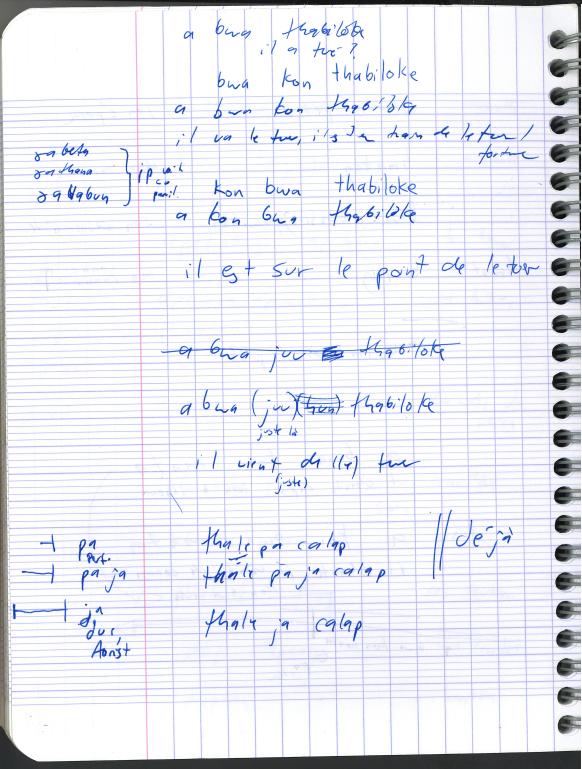
\includegraphics[width=\linewidth]{figures/vamale-170830-1005_67a}
%\label{fig:bwa_koon_notel}
%\caption{Field note extract concerning \textit{bwa koon} and \textit{koon bwa}}
%\end{figure}
%
%\begin{figure}
%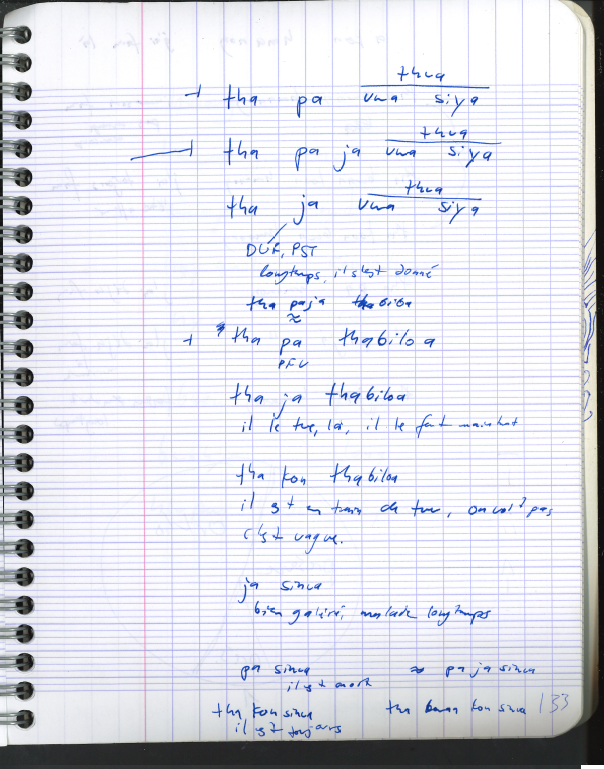
\includegraphics[width=\linewidth]{figures/vamale-170830-1005_67b}
%\label{fig:bwa_koon_noter}
%\caption{Field note extract concerning \textit{bwa koon} and \textit{koon bwa}}
%\end{figure}
%
%%todo{look at that}

 
 \section{Continuative and realis \textit{balan}}
 \label{sec:balan}
 \is{Aspect!\textit{balan}}
 
%TAM marking which uses \textit{balan} is a complex affair, because different meanings come together: continuity (despite obstacles) with durative verbs, but also realis and derived from this, immediacy to a salient moment in time.

The particle \textit{balan}, similarly to \textit{mu} described below, has more ambiguities than aktionsart can account for. Its interpretation depends on the context as well. The described event either: 

\begin{itemize}
	\item continues to happen (in some cases, despite an obstacle), 
	\item has just (unfortunately or finally) taken place or begun, 
	\item or will certainly and immediately happen.
\end{itemize}
 
\noindent The following section will first introduce \textit{balan} alone, with its two main meanings, continuative and realis, before addressing the common combinations with other aspect markers, as well as the less common ones. The section closes with a summary.
 
\textit{balan} may be a recent addition to the set of aspect markers, as speakers do not agree on the grammaticality of some of its uses, notably the combination with \textit{bo} (see \Cref{tab:balan}). One universally accepted use is that of \textit{bala-n} as a noun meaning \qu{piece of long object-\gl{nspec}}, as in \textit{balan o} \qu{piece of bamboo} and \textit{balan oot} \qu{length of string} (\ref{ex:balan_piece}). This \qu{bit} meaning allows a use of \textit{balan} as an attenuative particle, similar to \textit{xhwan}\slash\textit{xhwat} in (\ref{ex:balan_bit}) and (\ref{ex:balan_xhwan}). \is{Aspect!\textit{balan}!Attenuating}
 
 \ea
 \label{ex:balan_piece}
 % \langinfo{}{}{} 
 \gll  e=bo fe balan mwano-aen a=bo man nyako-ong\\
  1\gl{sg}=\gl{irr} take piece.length custom.cloth 3\gl{sg}=\gl{irr} rot on-1\gl{sg}.\gl{poss}\\
 \glt \qu{I'll take this piece of \textit{manou} [that you have given me as a greeting custom] and [will keep it forever so that] it will rot on me.} {[HC19:63]}
 \z
 
 
 \ea\label{ex:balan_bit}
 % \langinfo{}{}{} 
 \gll a=bo balan pala\\
  3\gl{sg}=\gl{irr} \gl{real}/bit speak\\
 \glt \qu{He will finally/a bit speak.} {[X10:55]}
 \z
 
 \ea\label{ex:balan_xhwan}
 % \langinfo{}{}{} 
 \gll a=bo xhwan pala\\
  3\gl{sg}=\gl{irr} bit speak\\
 \glt \qu{He will speak a bit.} {[X10:56]}
 \z
 
% \begin{itemize}
% 	\item balan
% 	\begin{itemize}
% 		\item a piece of a long object (\textit{wâng balan o} \qu{lit. boat piece bamboo, bamboo raft}, \textit{balan vaahit} \qu{tailless lizard [lit. bit of lizard]})
% 	\end{itemize}
% \end{itemize}

 Used as an aspect marker, \textit{balan} is more frequent in combination with other particles than alone, and \textit{balan} always comes second. A form combined with the progressive marker, \textit{kon balan}, and one with the irrealis one, \textit{bo balan} unambiguously mean \qu{has recently happened} and \qu{is just about to happen} respectively, though both are used rarely and judged ungrammatical by some speakers (especially \textit{kon balan}, perhaps because \textit{balan} expresses an immediate change of state, which contradicts \textit{kon}'s progressive meaning). Other aspectual particles precede \textit{balan} to add a sense of \qu{finally} (\textit{bwa balan}) or \qu{despite obstacles} (\textit{ja balan}). 
 
 Aktionsart also matters: durative verbs with \textit{balan} are either about to begin or have begun, but continue. Punctual verbs have either happened or are about to happen. Without context, certain verbs seem to have preferred interpretations. If the context suggests it, \textit{balan} can take an adversative function (\ref{ex:balan_adversative}). This example was elicited on the basis of a Nêlêmwa sentence with the same meaning using \textit{bara} \parencite[238]{bril_nelemwa_2002} and though the meaning \qu{unfortunately} was never found in free speech, speakers accepted it in an elicitation context.

\ea \label{ex:balan_adversative} 
\gll balan xhali sau-ng pwa-n yee	\\
 alas tear dress-1\gl{sg}.\gl{poss} on-\gl{nspec} tree	\\
\glt \qu{Unfortunately, my dress tore on a tree.}\\\relax 
[181016-jpgramm1, 00:12:56-00:12:58]
\z

\subsection{Continuative \textit{balan}}\is{Aspect!\textit{balan}!Continuative}
 Probably derived from the length-associated nominal meaning, is the aspectual use as a continuative. Used with atelic verbs, \textit{balan} can imply that the action happens despite a (potential) obstacle (\ref{ex:balan_han}), but may also refer to a lasting state (\ref{ex:balan_hmwaani}). This interpretation is only available with realis contexts, meaning that \textit{ja} \qu{\gl{prf}}, \textit{pa} \qu{\gl{prf}}, and controversial \textit{kon} \qu{\gl{prog}} are the only aspect markers that can combine with this continuative \textit{balan}. Example (\ref{ex:ja_balan}) combines \textit{balan}'s implication of an obstacle, with the resultative meaning of \textit{ja} to imply an expected hurdle. This is discussed in more detail in \sectref{ssec:ja_balan}. \textit{balan} is also found in the verb \textit{fe balan} \qu{to continue (lit. take length)}, and as an adverb meaning \qu{ever since}, see (\ref{ex:balan_since}).
 

 \ea\label{ex:balan_han}
 % \langinfo{}{}{} 
 \gll e=balan han\\
  1\gl{sg}=\gl{cont} walk\\
 \glt \qu{I keep walking (despite e.g. your calling me).} {[J2:39]}
 \z
 
 
 \ea\label{ex:balan_hmwaani}
 % \langinfo{}{}{} 
 \gll na i=s-ung tha balan hmwaani\\
  \gl{dem} \gl{def}.\gl{sg}=hand-1\gl{sg}.\gl{poss} \gl{ass} \gl{cont} like.this\\
 \glt \qu{It's my arm, it stays like this.} {[KG:139]}
 \z
 
 \ea\label{ex:ja_balan}
 % \langinfo{}{}{} 
 \gll e=ja balan jili wâng\\
  1\gl{sg}=\gl{prf} \gl{cont} build boat\\
 \glt \qu{Despite an expected holdup, I keep boat-building.} {[J2:43]}
 \z
 
 
 \ea\label{ex:balan_since}
 % \langinfo{}{}{} 
 \gll balan cel=e=xale-ko\\
  since when.\gl{real}=1\gl{sg}=see-2\gl{sg}.\gl{obj}\\
 \glt \qu{ever since I saw you} {[example sentence for the dictionary]}
 \z

 
 \subsection{Realis \textit{balan}}
 \is{Aspect!\textit{balan}!Realis}
 In irrealis situations, with punctual or telic verbs, and with atelic ones in the appropriate pragmatic context, \textit{balan} means something completely different: the realization of a situation.\footnote{Durative verbs do not carry the meaning \qu{just done}, but rather \qu{recently started and continuing}.} The continuative meaning discussed above maintains a situation, whereas this realis sense is concerned with change. With meanings ranging from \qu{this has just begun/come to happen} to \qu{finally}, the common denominator of non-continuative \textit{balan} is that the resulting construction is a realis one, or is so close to becoming one that it might as well already be. This is the reason why \textit{bo balan} is contested (see \sectref{ssec:bo balan}); it seems to be more widely accepted by younger speakers. \textit{bwa balan} ambiguously means either \qu{has recently begun and is still underway} and \qu{has practically begun}, probably both using the ambiguity of \textit{bwa} as both a realis and irrealis marker (\ref{sec:bwa}), and at least originally coming from hyperbole (\qu{I'm so close to doing it that I've practically begun}). However, neither of these explanations would work with \textit{bo}, which is explicitly irrealis and thus unlikely to be used here for hyperbole, as well as being unavailable for combinations with realis markers. The use of \textit{bo} with \textit{balan}, shown with its ambiguous meanings in  (\ref{ex:bo_balan}), may point at a development of \textit{balan} towards a more flexible meaning. %as in it's less striclty realis and more focused on the immediacy of limits 
 Interestingly, the ambiguity that \textit{balan} can express with regard to conceptual limits is shared by \textit{xhwan} \qu{almost, hardly}, and not unknown in other languages of the area (e.g. \textit{(k)u} \qu{\gl{prf}}, \citealt[206, 207]{bril_nelemwa_2002}). 
 
% A border close to the temporal reference point (almost finished/only just started?). There seems to be an ambiguity with durative verbs (\qu{a little bit}, see \ref{sec:bwa_balan} "bamboo raft"), but maybe this is a mistake of mine.

\begin{table}
	\caption{Overview of aspect marker combinations with \textit{balan}}
	\begin{tabularx}{\textwidth}{QQQQl}
	\lsptoprule
		\multicolumn{5}{c}{subject marker= \textit{b.}= verb}\\
		\textit{balan} & \textit{ja b.} & \textit{bwa b.} & \textit{kon b.} & \textit{bo b.}\\\midrule
		just done\slash about to do, continue to do, do despite  & finally do, do despite constraints & finally do (but not \textit{despite})& just begun\slash about to do & about to do\\
		\lspbottomrule
	\end{tabularx}
	\label{tab:balan}
\end{table}

\ea \label{ex:bo_balan} 
\gll gase=bo balan hmasan!\\
 1\gl{pl}.\gl{incl}=\gl{irr} \gl{real} bit arrive\\
\glt \qu{We will finally arrive!} {[X10:54]}
\z

\ea 
\gll a=bo balan pala\\
 3\gl{sg}=\gl{fut} \gl{real}/\gl{prf} speak\\
\glt \qu{He will finally/a bit speak.} {[X10:55]}
\z

\subsection{Finally, continuative: \textit{ja balan}}
\label{ssec:ja_balan}
\is{Aspect!\textit{balan}!Continuative}\is{Aspect!\textit{balan}!Realis}
The combination of \textit{ja} \qu{\gl{prf}} and \textit{balan} shows the oft-encountered temporal immediacy due to \textit{balan}, but \textit{ja}'s contribution is less clear. In examples (\ref{ex:jab1}) and (\ref{ex:jab2}), the meaning \qu{finally} is derived from \textit{ja}. In (\ref{ex:jab3}), \textit{balan} marks perseverance despite an obstacle, and \textit{ja} seems to mark that the obstacle is one that was known beforehand, perhaps relating to single \textit{ja}'s meaning of \qu{finally, after an observed period of becoming}.% (but keep in mind that \textit{balan} as a noun means \qu{a length of something}).

%\begin{table}
%	\caption{\textit{ja} balan}
%	\begin{tabular}{lllll}
%		aktionsart& word & before & \multicolumn{2}{c}{after}\\
%		\hline&&&&\\
%		\multirow{4}{1cm}{punctual}&arrive & about to & &just done\\
%		& finish & &done \emph{anyway}& \\
%		& die & & done \emph{anyway} &\\
%		&speak & finally & \emph{continue} to & \\
%		&&&&\\
%		\hline &&&&\\
%		\multirow{3}{1cm}{durative} &walk & & continue to &\\
%		&read & & & just begun, still happening\\
%		&build	&	& continue to &\\
%	\end{tabular}
%\end{table}

\ea\label{ex:jab1}
\gll a=ja balan pala\\
 3\gl{sg}=\gl{prf} \gl{cont} speak\\
\glt \qu{He continues to speak, he will finally speak.}\\
% \qu{Il continue à parler, il va parler}
\z


\ea\label{ex:jab2}
\gll 	e=ja balan fine i=tii	\\
	1\gl{sg}=\gl{prf} \gl{cont} read \gl{def}.\gl{sg}=book	\\
\glt	\qu{You (will) finally begin to read the book.}%\qu{T'as commencé à lire le livre.} \\ \qu{je suis sur le point de lire}	
\z


\ea
\gll gase={ja} balan hmasan!\\
 1\gl{pl}.\gl{incl}=\gl{prf} \gl{cont} arrive\\
\glt \qu{We are finally about to arrive, we have just arrived!}
%\qu{On est sur le point d'arriver, on vient d'arriver}
\z


An adversative meaning is not only achieved with \textit{balan} alone (\ref{ex:balan_adversative}), but also in combination with \textit{ja} \qu{\gl{prf}} (\ref{ex:ja_balan}). The meaning added to the simple adversative is one of foresight: the obstacle against which the predicate takes place is an expected one.

\ea
\gll e=ja balan han\\
 1\gl{sg}=\gl{prf} b. go\\
\glt \qu{I went on [despite my scheduled meeting].}
\z

\ea\label{ex:jab3} 
\gll 	e=ja balan jili wâng	\\
	1\gl{sg}=\gl{prf} b. build boat	\\
\glt \qu{I continue building my boat despite X.} {[J2:43]}%	\qu{Je continue à construire mon bateau (malgré des imprévus)}	
\z

\subsection{Finally: \textit{bwa balan}}
\label{sec:bwa_balan}
\is{Aspect!\textit{balan}!Realis}
\textit{bwa balan} marks an immediate temporal limit. For punctual verbs, this means either a recent end (\ref{ex:balanfinally}) or a recent beginning (\ref{ex:balanconv1}). For durative verbs, \textit{bwa balan} implies ongoing action (\ref{ex:balanconv2}). This is by far the most frequent form with \textit{balan}. \Cref{tab:bwabalan} summarizes the meanings with different verbs. 

\begin{table}
	\caption{bwa \textit{balan}}
	\begin{tabular}{llll}
	\lsptoprule
		Aktionsart& verb & future meaning & past\slash progressive meaning \\\midrule
		punctual&arrive & &recently done\\
		&finish & & recently done\\
		%	& die & & finally done? \\
		durative	&speak & about to& recently begun, \textit{still happening}  \\
		 &walk & about to  &recently begun, \textit{still happening}\\
		&read & & recently begun, \textit{still happening}\\
		&build	&	&  recently begun, \textit{still happening}\\
	\lspbottomrule
	\end{tabular}
\label{tab:bwabalan}
\end{table}


\ea\label{ex:balanfinally}
\gll gase={bwa} balan hmasan!\\
 1\gl{pl}.\gl{incl}=\gl{ipfv} bit arrive\\
\glt \qu{We finally arrived recently; we are about to finally arrive (this is so sure and immediate that we might as well have already arrived)!}%\qu{on est arrivé récemment}
\z

\ea\label{ex:balanconv1}
\gll e=bwa balan han\\
 1\gl{sg}=\gl{ipfv} b. go\\
\glt \qu{I am (finally about to be) leaving.}
\z

\ea\label{ex:balanconv2}
\gll 	e=bwa balan fine i=tii	\\
	1\gl{sg}=\gl{ipfv} b. read \gl{def}.\gl{sg}=book	\\
\glt	\qu{I have finally begun reading.}%\qu{J'ai commencé à lire}	
\z

While some verbs have a conventional interpretation, such as telic (\ref{ex:balanconv1}) and atelic (\ref{ex:balanconv2}), ambiguous, context-dependent cases are common (\ref{ex:balan_imm}), possibly because \textit{bwa} has many possible interpretations. %The combination \textit{bwa balan} is an example of the influence of the modified verb's aktionsart on TAM marker meaning.

\ea \label{ex:balan_imm}
\gll 	e=bwa balan jili wâng	\\
	1\gl{sg}=\gl{ipfv} b. build boat\\
\glt	\qu{I will begin building the boat (this is so sure that I have practically begun); I have begun.}%\qu{Je commence à construire le bateau, j'ai commencé}	
\z

\ea 
\gll a=bwa balan pala\\
 3\gl{sg}=\gl{ipfv} b. speak\\
\glt \qu{He has just spoken; he has begun to speak.} {[X10:51]}
\z
  %\todo{are the latter two not \textit{bwa balan}}


%However, the meaning is not completely up to its pragmatic context. Compare  (\ref{ex:bwa_balan_vi}) and (\ref{ex:bwa_vi}), repeated below: in both cases, a temporal border is close to the moment of speech. However, the reason why \textit{balan} makes the situation a past one in (\ref{ex:bwa_balan_vi}) is unclear. \textit{balan} probably contributes the notion of \qu{finally}, and \textit{bwa} possibly the meaning that it is close to the moment of speech.  %As \textit{vi} is durative, a future meaning of \textit{bwa} is not the only possibility. 
%
%\ea
%\ea\label{ex:bwa_balan_vi}
%
%\langinfo{}{}{} X10:50
%\gll e=bwa balan vi nyakoo-n
% 1\gl{sg} \gl{ipfv} \gl{cont} say \gl{obl}-3\gl{sg}.\gl{poss}
%\glt \qu{I have finally told him}
%
%
%\ea\label{ex:bwa_vi2}
%
%\langinfo{}{}{} X10:49
%\gll e=bwa vi nyakoo-n
% 1\gl{sg} \gl{ipfv} say \gl{obl}-3\gl{sg}.\gl{poss}
%\glt \qu{I will tell him}
%
%\z 
%Pragmatic context is important: comparing telic \textit{thabiloke} \qu{to kill} in (\ref{ex:bwa_balan-kill}) to atelic \textit{pala} \qu{talk} in (\ref{ex:bwa_balan-speak}), it appears that the telic verb is an action which finally happened, whereas with an atelic verb, a simple recent past is expressed. 
%
%\ea
%\ea\label{ex:bwa_balan-kill}
%
%\langinfo{}{}{} JR:17.8
%\gll ka e=bwa balan tha-bilo-a\textsuperscript{telic}
% \gl{cnj} 1\gl{sg} \gl{ipfv} b. with.strike-kill-3\gl{sg}.\gl{obj}
%\glt \qu{And finally I killed him.}
%
%\ea \label{ex:bwa_balan-speak}
%
%\langinfo{}{}{} X10:51
%\gll e=bwa balan pala\textsuperscript{atelic}
% 1\gl{sg} \gl{ipfv} b. speak
%\glt \qu{I have just spoken (I spoke very recently)}
%
%\z

\subsection{\textit{kon balan} \qu{about to, recently started}}
\is{Aspect!\textit{balan}!Realis}
Few speakers accept this form without context. If one needs to make clear that something has begun and is going on, this may be possible (\ref{ex:konb1}). Punctual verbs are even more contested, likely because of the progressive \textit{kon}.

\begin{table}
	\caption{kon \textit{balan}}
	\begin{tabular}{llll}
	\lsptoprule
		Aktionsart&Gloss of form & &\\\midrule
		\gl{punc}&arrive & &recently done\\
		&speak & \textit{finally} about to&  \\\addlinespace
		\gl{dur} &walk & \textit{finally} about to &  \\
		&read & &  recently begun\\
		&build	& &recently begun \\
	\lspbottomrule
	\end{tabular}
	\label{tab:kon_balan}
\end{table}

\ea
\gll 	e=kon balan jili wâng	\\
	1\gl{sg}=\gl{prog} \gl{real} build boat	\\
\glt	\qu{I have begun building the boat.}	
\z

\ea\label{ex:konb1}
\gll 	e=kon balan fine i=tii	\\
	1\gl{sg}=\gl{prog} \gl{cont} read \gl{def}.\gl{sg}=book	\\
\glt	\qu{(rare) I continue reading the book (it has just begun).}%\qu{(rare) Je continue à lire le livre}	
\z	

\subsection{\textit{bo balan} \qu{about to}}
\label{ssec:bo balan}
\is{Aspect!\textit{balan}!Realis}
The combination of \textit{bo} with \textit{balan} is not accepted by many older speakers, and is mostly used to unambiguously state on which side of the temporal border we are: the event is about to happen (\ref{ex:bobalan1}, \ref{ex:bobalan2}). One speaker translated an example with a realis meaning (\ref{ex:bobalan3}), but none were produced spontaneously.
%\begin{table}
%	\centering
%	\caption{bo \textit{balan}}
%	\begin{tabular}{llll}
%		punctual&arrive & \textit{finally} about to  &\\
%		& finish & & about to \\
%		& die & * & *   \\
%		&speak & \textit{finally} about to &  \\
%		&leave & \textit{finally} about to &  \\ &&&&\\
%		%durative	&read & & & recently begun, \textit{still happening}\\
%	durative	&build	& about to	& \\
%	\end{tabular}
%\end{table}

%A troubling detail is the meaning of durative \qu{fine} \qu{read, count}. The fact that an irrealis marker \textit{bo} can be interpreted as something realis is found nowhere else in the language. A tentative explanation would be that \textit{bo balan} is contested anyway, and that this confusing reading of it is due to the elicitation setting and the contrived nature of data collection.



	\ea\label{ex:bobalan1}
	[,am.bom.ba.lan.'pa.la]\\
	\gll a=bo balan pala\\
	 3\gl{sg}=\gl{irr} bit speak\\
	\glt \qu{He will finally speak.} {[X10:55]}
	\z
	
	\ea\label{ex:bobalan2}
	% \langinfo{}{}{} 
	%\langinfo{}{}{} 2017-09-01 Kito Nigai Thea
	\gll gase=bo balan hma-san!\\
	 1\gl{pl}.\gl{incl}=\gl{irr} \gl{prf} arrive-same.level\\
	\glt \qu{We will finally arrive!} {[X10:54]}
	\z
	
%	\a
%	
%	\langinfo{}{}{} [,em.bom.ba.'lan.hãn]
%	\gll e=\textbf{bo} balan han
%	 1\gl{sg} \gl{irr} \gl{cont} go
%	\glt \qu{I go on.}
%	
	
	\ea\label{ex:bobalan3}
	% \langinfo{}{}{} 
	\gll 	e=bo balan jili wâng	\\
		1\gl{sg}=\gl{irr} \gl{real} build boat	\\
	\glt	\qu{I begin building.} {[J2:44]}
	%\qu{Je commence à construire...}
	\z



 
\subsection{Summary: Combinations with \textit{balan}}
 While the chapter features a summarizing table at the end (\Cref{tab:aspect_combo}), % and this section an own table for \textit{balan} (\Cref{tab:balan_combo}), 
the following examples summarize the various functions of \textit{balan}. The data below were elicited explicitly as minimal examples and may present an over-simplified view. %, though the preceding section ``\sectref{sec:balan}" has done its best to muddle any convictions.
 
 \ea
 \gll 	e=fine i=tii	\\
 	1\gl{sg}=read \gl{def}.\gl{sg}=book	\\
 \glt	\qu{I read the book.}
 \z
 
 \ea
 \gll 	e=balan fine i=tii	\\
 	1\gl{sg}=\gl{real} read \gl{def}.\gl{sg}=book	\\
 \glt \qu{I just started reading a book, I am still reading it.}	%\qu{Trouvé un livre et tu lis tout de suite}	
 \z
 
 \ea
 \gll 	e=kon balan fine i=tii	\\
 	1\gl{sg}=\gl{prog} \gl{cont} read \gl{def}.\gl{sg}=book	\\
 \glt	\qu{(rare) I continue reading the book (it has just begun).}%\qu{(rare) Je continue à lire le livre}	
 \z
 
 \ea
 \gll 	e=bwa balan koin fine i=tii	\\
 	1\gl{sg}=\gl{ipfv} \gl{real} finish read \gl{def}.\gl{sg}=book	\\
 \glt	\qu{I have finished reading the book (just now).}%\qu{J'ai bien fini de lire}	
 \z

 \ea
 \gll e=bo balan koin fine i=tii\\ 
  1\gl{sg}=\gl{irr} \gl{real} finish read \gl{def}.\gl{sg}=book	\\
 \glt \qu{I am about to finish reading the book.}
 % \a
% 
% \gll 	e bwa koin fine i tii	
% 	1\gl{sg} \gl{ipfv} finish read \gl{def}.\gl{sg}=book	
% \glt	\qu{I am interrupting my reading (lit. I am stopping reading the book)}%\qu{Je m'arrête de lire (pour un moment)}	
% 
 \z
 
 Missing from this collection of examples is \textit{ja balan} \qu{finally \textit{balan}}, because the pragmatic context is so important that a representative example is impossible. 
 
%\begin{table}
% 
% 	\caption{Combinations with \textit{balan}: \textit{ja} \gl{prf}}
% 	\begin{tabularx}{\linewidth}{l|ll}
% 		\multicolumn{3}{c}{subject marker  \textit{balan}  verb}\\
% 		\hline &&\\
% 		verb & \textit{balan} & \textit{\textbf{ja} b.}\\
% 		&&\\
% 		\hline&&\\
% 		&just done / about to do  & do after long struggle, do/ \\
% 		&&achieve despite constraints\\
% 		\hline&&\\
% 		\textit{hma koon} \qu{find}& about to / just happened& \textbf{finally/despite X}: about to / just happened\\
% 		\textit{hmasan} \qu{arrive}& about to / just happened& \textbf{finally/despite X}: about to / just happened\\
% 		\textit{koin} \qu{end}& about to / just happened& \textbf{finally/despite X}: about to / just happened\\
% 		\textit{me} \qu{die}& about to / just happened& \textbf{finally/despite X}: about to / just happened\\
% 		\textit{pala} \qu{talk}& about to / still going& \textbf{finally/despite X}: about to / just happened\\
% 		\textit{han} \qu{go}& about to / still going& \textbf{finally/despite X}: about to / just happened\\
% 		\textit{fine} \qu{read}&about to / still going& \textbf{finally/despite X}: about to / just happened\\
% 		\textit{jili} \qu{build w/ wood}& about to / still going& \textbf{finally/despite X}: about to / just happened\\
% 	\end{tabularx}
% 	\label{tab:balan_combo}
%\end{table}

%\begin{table}
% \caption{Combinations with \textit{balan}: \textit{bwa} \gl{ipfv}, \textit{bo} \gl{fut}, \textit{kon} \gl{prog}}
% \begin{tabularx}{\linewidth}{l|lll}
% 	\multicolumn{4}{c}{subject marker  \textit{balan}  verb}\\
% 	\hline &&&\\
% 	verb & \textit{\textbf{bwa} b.} &  \textit{bo b.} & \textit{kon b.}  \\
% 	&&&\\
% 	\hline&&&\\
% 	& \textbf{finally} do /done & about to do & has just happened\\
% 	\hline&&&\\
% 	\textit{hma koon} \qu{find}&  \textbf{finally}: about to / just happened& about to& just now happened\\
% 	\textit{hmasan} \qu{arrive}& \textbf{finally}: about to / just happened&about to&just now happened\\
% 	\textit{koin} \qu{end}&  \textbf{finally}: about to / just happened&about to&just now happened\\
% 	\textit{me} \qu{die}& \textbf{finally}: about to / just happened&about to&just now happened\\
% 	\textit{pala} \qu{talk}&\textbf{finally}: about to / just happened&about to&just now happened\\
% 	\textit{han} \qu{go}& \textbf{finally}: about to / just happened&about to&just now happened\\
% 	\textit{fine} \qu{read}& \textbf{finally}: about to / just happened&about to&just now happened\\
% 	\textit{jili} \qu{build w/ wood} &\textbf{finally}: about to / just happened&about to&just now happened\\
% \end{tabularx}
% \label{tab:balan_combo2}
%\end{table}
 
 \section{Perfective \textit{pa (ja)} }
  \label{sec:pa ja}
  
The perfective marker \textit{pa}, marks the predicate as completed by the moment of speech (\ref{ex:pa}), or the relative temporal reference point, e.g. in stories. 

\ea \label{ex:pa} 
\gll cama=a=vi hapi a=pa xhwi-aman\\
 if=3\gl{sg}=say \gl{comp} 3\gl{sg}=\gl{prf} eat-thing\\
\glt \qu{If he says that he's already eaten [stop trying to feed him].} {[D3:78]}
\z

Contrary to most other aspectual markers, \textit{pa} is indifferent to aktionsart. \textit{pa} with an atelic verb means that this has already begun or finished depending on the context, and with a telic verb, that it has taken place. It is commonly translated as \textit{déjà} \qu{already} in French and stylistically often used in this sense. 
 
 Associating \textit{pa} with \textit{ja} \qu{\gl{prf}} (see \sectref{sec:ja}) adds the information that the completion took some time, or was long awaited, as in (\ref{ex:pa_ja1}), or that whatever is marked has happened some time ago, as in (\ref{ex:pa_ja2}). This is by far the most common combination with \textit{pa}.
 

 \ea \label{ex:pa_ja1}
 %\langinfo{}{}{}  
 \gll le=ja vatipwe-mwa kon ya tha pa ja me-a go tha le=ja thuat-mwa moo ka li=xhaomu ja tha le=ja ha-mwa-me \\
  3\gl{pl}=\gl{prf} drop-\gl{rep} because 3\gl{sg} \gl{ass} \gl{prf} \gl{prf} die-3\gl{sg} then \gl{ass} 3\gl{pl}=\gl{prf} emerge-\gl{rep} stay \gl{sbj} \gl{def}.\gl{pl}=elder \gl{prf} \gl{ass} 3\gl{pl}=\gl{prf} go-\gl{rep}-\gl{dir.cp}\\
 \glt  \qu{They were released [again] because he was already dead, and they came out of prison [again] and came back.} {[HC1:32]}
  \z
 
 
 \ea\label{ex:pa_ja2}
 \gll ma le=ta ma le=xale-a koma le=fe-a ma le=ta ma le=fe-a, ya pa ja me-a  \\
  \gl{com} 3\gl{pl}=go.up \gl{com} 3\gl{pl}=see-3\gl{sg} so.that 3\gl{pl}=take-3\gl{sg} \gl{com} 3\gl{pl}=go.up \gl{subr} 3\gl{pl}=take-3\gl{sg} 3\gl{sg} \gl{prf} \gl{prf} die-3\gl{sg} \\
\glt \qu{And they went up, saw him, in order to catch him, they went up to catch him, he (however) was already dead.} {[HC1:29]} 
 \z

As illustrated in (\ref{ex:paja_cipe}), \textit{pa} (with its frequent companion \textit{ja}) can precede the subject index, though this is rare. This is also attested for \textit{bwa} \qu{\gl{ipfv}}; both are only found in negated contexts. The semantic difference achieved, like with \textit{bwa}, is that \textit{cipe pa ja jili bwaakala} \qu{I don't already build boats} does not clarify whether the subject ever built boats, whereas \textit{pa ja} in the first position adds a sense of achievement to the statement \qu{I don't build boats}, i.e. \qu{my building days are done}.

\ea \label{ex:paja_cipe}
\gll pa ja cip=e jili bwaakala\\
 \gl{prf} \gl{prf} \gl{neg}=1\gl{sg} build.with.wood outrigger.canoe\\
\glt \qu{I already don't build boats anymore.} [B2:144]
\z

\section{Perfect \textit{ja} \qu{finally}}
\label{sec:ja}
\is{Aspect!\textit{ja} \qu{finally}}
The Bwatoo cognate of this form, \textit{je}, is glossed as ``accomplished" \parencite[56]{rivierre_bwatoo_2006}. For atelic verbs, \textit{ja} expresses the expected, or long-awaited beginning of the action, as in (\ref{ex:ja_hantabo}), (\ref{ex:ja_hup}), and (\ref{ex:ja_seada}). Note the verb \textit{jake} \qu{measure, weigh}, which may be related.


\ea\label{ex:ja_hantabo}
\gll ...hê a={ja} han tabo pwan bwa-n, koin a={ja} fe-ta-mwa-me-a\\
 yes 3\gl{sg}=\gl{prf} go sit on head-3\gl{sg}.\gl{poss} then 3\gl{sg}=\gl{prf} take-go.up-\gl{rep}-\gl{dir.cp}-3\gl{sg}.\gl{obj}\\
\glt \qu{Yes, he\textsubscript{i} eagerly climbs to sit on his\textsubscript{ii} head, then he\textsubscript{ii} takes him\textsubscript{i} home.} {[HC2:26] (see \Cref{text:squid2})}
\z

%\ea
%
%\langinfo{}{}{} HC2:27-28 (context for following)
%\gll ...lu hmaca-mwa-me can hmeewan, ma xhasat nyada-mwa siibwi phwâêû.
% 3\gl{du} arrive-\gl{rep}-\gl{dir.cp} in sand \gl{com} jump send-\gl{rep} rat dry.land 
%\glt \qu{The two arrive on the beach and the rat jumps unto dry land.}
%

\ea\label{ex:ja_hup}
\gll go cama i=ibwen a={ja} hup- a=kon {ja} hup-wa-e can we...\\
 then concerning \gl{def}.\gl{sg}=squid 3\gl{sg}=\gl{prf} go.down 3\gl{sg}=\gl{prog} \gl{prf} go.down-\gl{rep}-\gl{dir.cf} in water\\
\glt \qu{Then, when the squid finally goes down back into the water\ldots}\\ \qu{Then, once the squid had gone back into the water [and the rat thought himself at a safe distance to mock him]...} {[HC2:29]}
\z

\ea \label{ex:ja_seada}
\gll siibwi tha pa me-a. tha=a=pa {ja} sea-da\\
 rat \gl{ass} \gl{prf} die-3\gl{sg} \gl{ass}=3\gl{sg}=\gl{prf} \gl{prf} gaze-up \\
\glt \qu{The rat is dead. He ended up gazing upwards.} {[HC2:40]}
\z

\ea \label{ex:ja_end}
\gll cama ibwen tha=a={ja} hup-wa, tha ja koin mwa \\ %\textsuperscript{temp. deix}
 concerning squid \gl{ass}=3\gl{sg}=\gl{prf} go.down-\gl{rep} \gl{ass} \gl{prf} end \gl{rep}\\
\glt \qu{And the squid, he went back down. This is the end.}\\
\qu{The squid has gone down, thus it has ended.} {[HC2:39-40]}
\z

With telic verbs, \textit{ja} marks that something finally happens, be it that it was actively anticipated (\textit{tha jaa koin} \qu{it's finally over}) or (\ref{ex:ja_vwa}), or that it was expected and inevitable like one's own departure from a social situation: \textit{e bwaa ja han} \qu{I'm about to finally leave}. The latter function likens it to \textit{pa} (\sectref{sec:pa ja}), with which it often associates. Whereas \textit{pa} only marks that the action is completed by the temporal point of reference, \textit{ja} adds a sense of \qu{finally}, similar to Comrie's ``perfect of result" \parencite[58]{comrie_aspect_1981}. This also applies to the result of a natural process: \textit{bwaam, tha jaa xhopwe-go!} \qu{My, you've grown!}. Stylistically, \textit{ja} may to be used to close a scene, see (\ref{ex:ja_end}) and Swamp Hen's takeoff (\ref{ex:ja_ta}, \ref{ex:ja_ta2}), where \textit{ja} marks the final leave of the swamp hen; we do not see her again. It cannot be used to describe the death of a person, as this would suggest that their death was expected. Given that \textit{ja} expresses the result of an observed process and introduces a situation that is relevant for the time of reference (the present in direct situations, the narrative time in stories), \textit{ja} will be labelled as ``perfect". 

%Means that whatever follows is now over, does not occur alone to describe present situations
%Telic:

\ea\label{ex:ja_vwa}
\gll ...go a={ja} vwa mwa me ka i=siibwi.\\
 then 3\gl{sg}=\gl{prf} do \gl{rep} die \gl{sbj} \gl{def}.\gl{sg}=rat\\
\glt \qu{Then he killed him.} {[HC2:38]}% ("il l'a tué")}
\z 

\ea\label{ex:ja_ta}
\gll go tha=a={ja} ta-mwa-me\\
 then \gl{ass}=3\gl{sg}=\gl{prf} go.up-\gl{rep}-\gl{dir.cp}\\
\glt \qu{And then it went home.} {[HC2:12]} 
\z

\ea\label{ex:ja_ta2}
\gll ya tha {ja} thêên thêên ta-mwa-me\\
 3\gl{sg} \gl{ass} \gl{prf} fly fly go.up-\gl{rep}-\gl{dir.cp}\\
\glt \qu{Flew home right away.} {[HC2:13]} 
\z

\section{Present perfective \textit{kon ja}}
In combination with \textit{kon} \qu{\gl{prog}}, \textit{ja} expresses something that is done by the moment which \textit{kon} designates (\ref{ex:konja}). 

\ea \label{ex:konja}
\gll putain yo m=e th=e=kon ja vwa i=\textit{signe}\\
 fuck 1\gl{sg} \gl{subr}=1\gl{sg} \gl{ass}=1\gl{sg}=\gl{prog} \gl{prf} do \gl{def}.\gl{sg}=sign\\
\glt \qu{Rats, I should have given [him] a sign by then.} {[KG:492]}
\z 
%\ea 
%\ea
%
%\langinfo{}{}{} Fable of the North Wind and the Sun, V1:4
%\gll ka i wabataan a \textbf{ja} juu cika mwa\textsuperscript{anymore?} wîîn
% \gl{cntr} \gl{def}.\gl{sg}=north.wind 3\gl{sg} \gl{prf} really \gl{neg}.\gl{exist} \gl{rep} strength
%\glt \qu{And the North Wind had no strength left.}
%
%
%\a
%
%\langinfo{}{}{} V1:5 (for context)
%\gll ka i xat a bwa nyoot mwa\textsuperscript{temp. deix?} nya wîîn
%  \gl{cntr} \gl{def}.\gl{sg}=sun 3\gl{sg} \gl{ipfv} come.out \gl{rep} give strength
%\glt \qu{And the Sun shone strongly}
% 
%
%\a
% 
%\langinfo{}{}{} V1:5 (for context)
%\gll ka i apuli a \textbf{ja} juu uti saun
%  \gl{cntr} \gl{def}.\gl{sg}=man 3\gl{sg} \gl{prf} really take.off cloak   
%\glt \qu{And the man took off his cloak immediately.}
% 
%\z
 
 \section{Frequentative and iterative \textit{mu}}
  \label{sec:mu}	
 \textit{mu} is a versatile particle, and can mean \qu{as well; all along, during a certain time; at selected moments over a long period of time}. \is{Aspect!Frequentative \textit{mu}}Depending on the aktionsart and the aspectual context of the verb, \textit{mu} can take on frequentative functions (\ref{ex:mu_freq}): this concerns telic verbs in general (\ref{ex:mu_aube_tel} and \ref{ex:mu_taemwi}), and countable, finished events (\ref{ex:mu_bwa1} and \ref{ex:muoften1}).% \textit{mu} reacts not only to telicity. An atelic event can have happened all along over a period of time, or, if the context is understood to be present instead of past, the atelic event is happening as we speak, little by little.
 
% \ea
 \ea\label{ex:mu_aube_tel}\label{ex:mu_freq}
 \gll m=e xa-vwa hmwata i=bee-ng a=mu xhajake\\
  \gl{irr}=1\gl{sg} \gl{hab}-make starchy.cake \gl{def}=brother-1\gl{sg}.\gl{poss} 3\gl{sg}=\gl{freq} eat.starchy\\
 \glt \qu{Whenever I make a yam cake, my brother eats it.} {[X10:40]}
  \z
 
 \ea\label{ex:mu_taemwi}
 \gll calibeen goakan e=mu taemwi li=nyu \\
  sometimes moment 1\gl{sg}=\gl{freq} catch \gl{def}.\gl{pl}=fish\\
 \glt \qu{I catch fish every time.} {[X10:42]}
 \ex\label{ex:mu_bwa1}
 \gll e=bwa mu majit\\
  1\gl{sg}=\gl{ipfv} \gl{freq} rest\\
 \glt \qu{I sleep from time to time.} {[J4:31]}
 \ex\label{ex:muoften1}
 \gll ca i=nyan-mwa xahan le=mu sivu sikaa \\
  in \gl{def}.\gl{sg}=inside-house  over.there 3\gl{pl}=\gl{freq} blow cigarette \\
 \glt \qu{They have the habit of smoking in this room over there.} {[X10:44]}
 \z
 \is{Aspect!Iterative \textit{mu}}
 Another function is iterative, with durative verbs (\ref{ex:mu_it}). There is a difference in meaning with past and present situations, i.e. an ongoing action with \textit{mu} is yet incomplete and evolving bit by bit (\ref{ex:mu}), whereas a past action happened several times or bit by bit (\ref{ex:mu_bwa2}). With a stative verb (\ref{ex:muxhwatin}), it may mean a development, as with \textit{e-} \qu{\gl{mid}} (\sectref{ssec:MID_unbounded}).
 
% \ea
 \ea\label{ex:mu}\label{ex:mu_it}

 \gll a=mu hnuut\\
  3\gl{sg}=\gl{iter} go.downstream\\
 \glt \qu{He is (still) going down.} {[J4:27]}
 \ex\label{ex:mu_bwa2}
 \gll e=bwa mu tena ha-mwa\\
  1\gl{sg}=\gl{ipfv} \gl{iter} hear go-\gl{rep}\\
 \glt \qu{I heard about it all along.} {[Tipije]}
 \ex \label{ex:muxhwatin}
 %\langinfo{}{}{} \textit{mu}, an iterative marker for durative verbs
 % vamale-180929-ddgrammaire-04 00:40:55 -- 00:41:46
 \gll 	a=mu xhwatin	\\
 	3\gl{sg}=\gl{iter} small	\\
 \glt	\qu{It is shrinking.}	
 \z
  
However, \textit{mu} can also have additive meanings (for states, as in (\ref{ex:mu_too})). Note that this is only attested in combination with \textit{pa} \qu{already}.\is{Aspect!Additive \textit{mu}}\largerpage
%\label{ex:mu_add}
	\ea\label{ex:mu_too}\label{ex:mu_add}
	\gll tha pa mu hman-ong\\
	 \gl{ass} already \gl{add} hungry-1\gl{sg}\\
	\glt \qu{I, too, am hungry already.} {[J4:30]}
	\ex\label{ex:mu_as-well}
	\gll e=paa mu majit\\
	 1\gl{sg}=\gl{prf} \gl{add} rest\\
	\glt \qu{I, too, am already asleep.} {[J4:32]}
	\z

Some uses are ambiguous, with durative, atelic verbs that can be understood as countable events (\ref{ex:muoften2}). The meanings of \textit{mu} are summarized in \Cref{tab:mu}.
 \ea \label{ex:muoften2}
\gll e=mu se\\
 1\gl{sg}=\gl{iter}/\gl{freq} cry\\
\glt \qu{I cry (often; still).} {[X10:92]}
\z


\begin{table}
	\centering
	\caption{Shades of \textit{mu}}
	\begin{tabularx}{\textwidth}{llQl}
		\lsptoprule
		& \textit{mu} & \textit{bwa mu} & \textit{pa mu} \\
		\midrule
		atelic  &  still, every time (\ref{ex:muoften1}, \ref{ex:muoften2}) & several times over time (opt. with \textit{hamwa}) (\ref{ex:mu_bwa1}, \ref{ex:mu_bwa2})     &  also (\ref{ex:mu_add}) \\
		telic  & every time (\ref{ex:mu_aube_tel})&     \\
\lspbottomrule
	\end{tabularx}
	\label{tab:mu}
\end{table}


%\begin{table}[]
%	\centering
%	\caption{My captionxx}
%	
%	\begin{tabular}{lllll}
%		& \multicolumn{2}{c}{mu}      & pa mu & bwa mu           \\
%		\midrule
%		& not now                  & now   &              &                     \\
%			\midrule[0.8mm]
%		durative     & often, habit             & still & already, too & from time to time   \\
%		not durative & every time (catch fish?) &       &              &                     \\
%		telic        & every time               & ?     &              & all along (+hamwa)? \\
%		dynamic      &                          &       &              &                    
%	\end{tabular}
%\label{tab:mu3}
%\end{table}




%\begin{comment}
%
%Calibeen
%
%\ea
%
%\gll the xaje sake calibeen
% \gl{ass}.1\gl{sg} eat.juicy jackfruit often
%\glt \qu{I often eat jackfruit}
%
%\z
%
%\end{comment}

\section{Combinations}
 \label{sec:asp_combo}
 
 Vamale aspect markers can be combined to create more complex, and sometimes altogether different meanings. See \Cref{tab:aspect_combo} for an overview of combinations.
 Combinations are in some cases preferred to the lone form (especially with \textit{ja} \qu{\gl{prf}} and \textit{balan} \qu{\gl{cont}}), and may change the overall meaning significantly. %While some aspect markers, especially \textit{bwa}, can occur in a position left of the subject marker, combinations only occur between particles in the canonical position between the person marker and the predicate. 
 
 \begin{table}
	\small
 	\caption{Overview of aspectual markers and their meanings}
 	\begin{tabularx}{\textwidth}{lllQlQ}
 		\lsptoprule
 		     &       & \multicolumn{2}{l}{Atelic example}                  & \multicolumn{2}{l}{Telic example}\\
 		Form & Gloss & \multicolumn{2}{l}{\textit{majit} \qu{to lie down}} & \multicolumn{2}{l}{\textit{hma} \qu{arrive}}\\
 		\midrule
 		\textit{balan} & \gl{cont} & a b. majit &\qu{s/he keeps sleeping}& a b. hma& \qu{s/he will immediately\slash has just arrived}\\
 		\textit{bo} & \gl{irr}/\gl{fut}& a b. majit& \qu{he will sleep}& a b. hma& \qu{s/he will arrive}\\
 		\textit{bwa} & \gl{ipfv} & a b. majit& \qu{he still sleeps} & a b. hma& \qu{s/he will arrive (certain)}\\
 		\textit{ja} & finally & a j. majit &\qu{s/he finally sleeps} & a j. hma & \qu{s/he has finally arrived}\\
 		\textit{kon} & \gl{prog} & a k. majit & \qu{s/he is sleeping} & * &\\
 		%	koin & semelfactive & k. a majit &\qu{while he sleeps}& koin a hma& xx?\\ 
 		\textit{mu}& \gl{iter}, \gl{freq} & a m. majit &\qu{s/he sleeps regularly\slash little by little} & a m. hma& \qu{s/he arrives (every time)}\\ 
 		%mwa & repetition & a majit mw. &\qu{he sleeps again / on top of that} & a hma mw.& \qu{he has arrived again / on top of that}\\
 		\textit{pa} & \gl{prf} & a p. majit& \qu{s/he has (already) slept}& a p. hma& \qu{s/he has (already) arrived}\\
 		\lspbottomrule
 	\end{tabularx}
 	\label{tab:aspect}
 \end{table}
 
  Combinations are not possible between all markers. For instance, perfective \textit{pa} \qu{\gl{prf}} and imperfective \textit{bwa} cannot be combined, nor \textit{bo} \qu{\gl{irr}} and the realis \textit{bwa} \qu{\gl{ipfv}}. Reversing the order of the markers is rarely possible, though when it is, it always affects the meaning. Several combinations are more frequent than each of their components, especially with \textit{balan} \qu{\gl{cont}} (see \sectref{sec:balan}). The reason for these differences in aspect marker behavior may have historical reasons.
 
\begin{table}
	\caption{Aspect marker combinations}
	\footnotesize
	\begin{tabularx}{\linewidth}{lll >{\raggedright}p{\widthof{X-ing}} >{\raggedright}p{\widthof{before}}  QQQ}
		\lsptoprule
	    First & & \multicolumn{6}{c}{Second form}\\
	    form &Gloss&\textit{bo} & \textit{bwa} & \textit{kon} & \textit{balan}  & \textit{ja} & \textit{mu}\\\midrule
		\textit{bo} & \gl{fut}, \gl{irr} &&*&*&about to happen& will/would finally&will/would from time to time\\
		\textit{bwa} & \gl{ipfv}&*&&still X-ing since before&finally about to&finally X-ing (in general, not necessarily right now)& still X-ing from time to time\\
		\textit{kon} &\gl{prog}&*&still X-ing right now&&has just happened&X-ing at last& X-ing little by little\\
		\textit{balan} &\gl{cont}, \gl{real} &*&*&&*&*&* \\
		\textit{pa} & \gl{prf}&*&*&*&& finally completed after a known period&* \\
		\textit{ja} &\gl{prf}&*&*&finally X-ing&finally completed after a known period&*&finally from time to time \\
		\textit{mu} &\gl{freq}, \gl{add}, \gl{iter}&*&*&*&*&*& \\
		\lspbottomrule
	\end{tabularx}
	\label{tab:aspect_combo}
\end{table}



% i want this section to say how i work and why, and what problems and particularities i encountered in the field. 

\chapter{Simple clauses} 
\label{ChapterSimpClaus} 
\is{Clauses!Simple clauses}
This chapter treats simple clauses and the elements they contain, and describes how a matrix clause is formed. As this is the first chapter to discuss matrix clauses and the elements that appear outside of verb and noun phrases, particles such as assertive \textit{tha} (\sectref{sec:ass}) and the repetitive marker \textit{mwa} (\sectref{sec:mwa}) are described here, as well as the discourse markers \textit{go} (\sectref{ssec:discourse go}) and \textit{ka} (\sectref{discourse ka}). Word order is also explicitly mentioned here for the first time (\sectref{sec:alignment}), as this is the first chapter to look at the domain of the clause. %will first introduce Vamale word order and describe the prevalent alignment patterns, before describing
Simple clauses have one main predicate, one subject, one TAM contour, and share a single polarity. A simple clause may contain several verbs, in the case of serial verb constructions (\sectref{sec:SVC}). The main clause types are declarative (\sectref{sec:decl_clauses}), interrogative (\sectref{sec:Interr_clauses}), imperative and prohibitive clauses (\sectref{sec:IMP_clauses}). A brief section addresses equative clauses, which in absence of a copula juxtapose two nouns (\sectref{ssec:Verbless_clauses}). %\sectref{sec:} on declarative xx
As the assertive \textit{tha} is discussed in this chapter, other modal particles and constructions are mentioned as well (\sectref{sec:Modality}). Most of them involve subordination, which is described separately again in \sectref{ssec:ma}. A typical sentence looks as follows:
\begin{center}
PN= TAM= root -\gl{obj}/-\textit{ke} (\gl{art}=) \gl{obj} (\textit{ka}= (\gl{art}=) NP\textsubscript{subject})
\end{center}
\noindent Noun phrases do not necessarily take articles, and argument expression through noun phrases is optional, as indexing on the verb already carries this information.

\section{Word order}
\label{sec:alignment}
\is{Word order}
\is{Clauses!Word order}
Word order in Vamale does not change across clause types. Vamale is head-first and usually VOS, though fronted, bi-clausal constructions are common: S, VO. The verb always precedes the object, and the traditionally non-marked order expects the subject after the noun. Oblique arguments tend to follow objects (\ref{ex:obj_then_obl}), but pragmatic choices can invert the unmarked order (\ref{ex:obl_then_obj}). In general, the earlier a constituent is introduced, the more marked it is. %The subject is often fronted, but may then still occur after the verb, indicating that a fronted subject is not a constituent of the clause.\footnote{Prosodically, too, the fronted subject has an own contour, which yields two intonation units: the fronted subject, and the clause.} Fronting can be used to focus on any constituent, a resumptive morpheme remains in the matrix clause.



\ea\label{ex:obj_then_obl}
\gll e=holeke {\ob}sikaa{\cb}\textsuperscript{obj} {\ob}nyasi i=apuli a= xhwata{\cb}\textsuperscript{obl}\\ 
 1\gl{sg}=thank.for cigarette \gl{ben} \gl{def}.\gl{sg}=man \gl{rel}= bald\\ 
\glt \qu{I thank the bald man for the cigarette.}
 \z
 
\ea\label{ex:obl_then_obj}
\gll e=holeke nyasi-m li=fati a= go=vi\\ 
 1\gl{sg}=thank.for \gl{ben}-2\gl{sg}.\gl{poss} \gl{def}.\gl{pl}=word \gl{rel}= 2\gl{sg}=say\\ 
\glt \qu{I thank you for the words.} {[B2:94]}
\z

%\a
%
%\gll  yo e=bwa ja fa-xaleke i ye nyako i apuli
% 1\gl{sg} 1\gl{sg} \gl{ipfv} ja \gl{caus}-see \gl{def}.\gl{sg}=tree \gl{obl} \gl{def} man
%\glt \qu{I have been making the man look at the tree.}
%


%\todo{I would add a gloss line just beneath the Vamale elements}
%%todo{test examples}
The basic word order VOS is generally more common with older speakers, while younger generations often front the subject. Stative verbs, especially with inanimate arguments such as in (\ref{ex:xhong}), seem to be exempt from the fronting mentioned above, regardless of the speaker demographic. With animate arguments, fronting is especially common, especially when the agent is stressed. Strategies to make the subject less salient to the listener include using the VOS order, as well as not mentioning the subject, and fronting the object, as in (\ref{ex:fronted_obj}).

\ea \label{ex:xhong}
\gll sinu i=xho-ng\\ 
 ill \gl{def}.\gl{sg}=leg-1\gl{sg}.\gl{poss}\\ 
\glt \qu{My leg hurts.}
\z


	
%	\ea\label{ex:itrs_sbj}
%	
%	\gll e=ta ka yo
%	 1\gl{sg} go.up \gl{sbj} 1\gl{sg}
%	\glt \qu{I go up}
%	
%	
%	\ea\label{ex:1sg_sbj}
%	
%	\gll yo, e=xale-ko (ka yo)
%	 1\gl{sg} 1\gl{sg} see-2\gl{sg}.\gl{obj} \gl{sbj} 1\gl{sg}
%	\glt \qu{Me, I see you}
%	
%	\ea
%	
%	\gll go ta
%	 2\gl{sg} go.up
%	\glt \qu{You go up}
%	
%	\ea\label{ex:2sg_sbj}
%	
%	\gll go, go xale-o
%	 2\gl{sg} 2\gl{sg} see-1\gl{sg}.\gl{obj}
%	\glt \qu{You, you see me}
%	
\ea \label{ex:alignment}	
\label{ex:fronted_obj}
	\gll go, e=xale-ko \\ 
	 2\gl{sg} 1\gl{sg}=see-2\gl{sg}\\ 
	\glt \qu{You, I see you.}
	\z
	
	\ea\label{ex:non-fronted_obj}
	\gll e=xale-ko \\ 
	 1\gl{sg}=see-2\gl{sg}.\gl{obj}\\ 
	\glt \qu{I see you.}
	\z 
	
%\footnotetext{Formerly preferred, see \Cref{text:tipije}}
%\footnotetext{Preferred now}

%Stative verbs use different morphemes to mark their subjects, and those suffixes are not identical (although very similar) to object-marking suffixes found on transitive verbs, as in (\ref{ex:1sg_sbj}). Inanimate participants are neither marked with object suffixes nor stative subject suffixes, but otherwise behave like animate ones, i.e. inanimate noun phrases are flagged as subjects and obliques. Both non-specific objects (irrespective of animacy) and inanimate non-specific stative subjects are marked with \textit{-n} \qu{\gl{nspec}} on the verb. This distributional similarity between inanimate objects and stative subjects, as well as the formal similarity of the -\gl{S\textsubscript{P}} and -\gl{p} suffixes raises questions concerning an animate/inanimate split. 
%This means that Vamale uses a split-S system in its person marking, marking transitive verbs like active intransitive ones, distinguishing stative verbs from the former set, and marking objects yet differently. A table summarizing the forms is given in \Cref{ChapterVerbs} (see \Cref{tab:markers2}), and is repeated here as \Cref{tab:markers3}.

%\begin{table}
%	\centering
%	\caption{Subject and object markers for active and stative verbs}
%	\label{tab:markers3}
%	\begin{tabular}{lllll}
%		&	Free form	& \gl{a}=/\gl{S\textsubscript{A}}= & -\gl{S\textsubscript{P}} & -\gl{p}\\
%		1\gl{sg} & \textit{io} & \textit{e} & \textit{-o(ng)} & \textit{-o} \\
%		1\gl{du}.\gl{incl}& \textit{gasu} & \textit{gasu} & \textit{-gasu} & \textit{-kaeu}\\
%		1\gl{pl}.\gl{incl} & \textit{gaa/gase} &\textit{ga(se)}&\textit{gaa}&\textit{-kaa}\\
%		1\gl{du}.\gl{excl} & \textit{abu} & \textit{abu} & \textit{-abu} & \textit{-(a)bu}\\
%		1\gl{pl}.\gl{excl} & \textit{abe}& \textit{abe} & \textit{-abe} & \textit{-(a)be}\\
%		2\gl{sg} & \textit{go} &\textit{go} & \textit{-go} & \textit{-ko}\\
%		2\gl{du} & \textit{gau} & \textit{gau} & \textit{-gau} & \textit{-kau}\\
%		2\gl{pl} &\textit{gavwe}& \textit{gavwe} & \textit{-gavwe} & \textit{-kavwe}\\
%		3\gl{sg} & \textit{ia} & \textit{a} & \textit{-(e)a} & \textit{-(e)a}\\
%		3\gl{du} & \textit{lu} &\textit{lu} & \textit{-lu} & \textit{-lu}\\
%		3\gl{pl} & \textit{le} & \textit{le} & \textit{-le} & \textit{-le}\\
%	\end{tabular}
%\end{table}
%

%\ea
%%\a
%%
%%\gll yo, a xale-o ka ya
%% 1\gl{sg} 2\gl{sg} see-1\gl{sg} \gl{agt} 3\gl{sg}
%%\glt \qu{Me, he saw me}
%% 
%
%\a
%
%\gll a xale-o ka i pupwaale
% 3\gl{sg} see-1\gl{sg} \gl{cnj} \gl{def} Caucasian
%\glt \qu{The white guy sees me}
%
%
%
%\a
%
%\gll a-xale-a i pupwaale ka i daahma
% 3\gl{sg} see-3\gl{sg}.\gl{obj} \gl{def} Caucasian \gl{agt} \gl{def} chief
%\glt \qu{The chief sees the White guy}
%
%
%\a
%
%\gll *a xale-a i pupwaale i daahma
% 3\gl{sg} see-3\gl{sg}.\gl{obj} \gl{def} Caucasian \gl{def} chief
%\glt \qu{(The chief sees the White guy)}
%
%
%\a
%
%\gll a majit i pupwaale
% 3\gl{sg} rest \gl{def} Caucasian
%\glt \qu{The white guy sleeps}
%
%\z 

%\ea 
%\ea
% 
%\gll a xale-o\textsuperscript{Sᵃ}
% 3\gl{sg} see-1\gl{sg}.\gl{obj}
%\glt \qu{He sees me.}
% 
%
%\ea
% 
%\gll sinu-ong\textsuperscript{Sᵖ}
% sick-1\gl{sg}.\gl{sbj}
%\glt \qu{I am sick/dying.}
% 
%
%\ea
% 
%\gll a majit
% 3\gl{sg} sleep
%\glt \qu{He sleeps.}
%
%
%\ea
% 
%\gll {*}a thathe
% 3\gl{sg} wound
%\glt \qu{(he is wounded)}
% 
%\z

%Nowadays, the word order is more often A, a=V P than a=V P ka A, so that there is no difference between A and S, and we have a nominative/accusative system for nouns as well.


\section{Clause types}
\label{sec:clause_types}
\is{Clause types}

Main clauses in this grammar are those who routinely appear alone and cannot be governed by another clause without subordinating morphology. This includes declarative clauses both with verbs and equative ones with nouns, as well as interrogative, imperative, and prohibitive clauses.
The morphosyntax of main (or matrix) clauses is the same as that of most subordinate ones, a topic discussed in further detail in \Cref{ChapterSub}. Exceptions to this are imperative clauses, which do not index the subject on the verb. 


\subsection{Declarative clauses}
\label{sec:decl_clauses}
\is{Clauses!Declarative clause}
Declarative clauses are the most common ones in Vamale. They usually contain a subject, either present as a proclitic subject marker, for active verbs and nominal predicates, or as a suffix, for stative verbs with an animate subject, and which can always be expressed as a free noun phrase after the verb phrase, flagged with \textit{ka} \qu{\gl{sbj}}, or fronted (in which case it is its own clause, prosodically distinct and syntactically not integrated). Exceptions which do not need a subject are impersonal verbs like \textit{vwasoon} \qu{impossible} (discussed in \sectref{sec:ZeroTrans}), and imperative clauses.

\subsubsection{Discourse marker \textit{ka}}
\label{discourse ka}
\is{Discourse markers!Discourse marker \textit{ka}}

Putting \textit{ka} at the end of a sentence is a question to the listener: do you follow? This \textit{ka} (\ref{ex:coorka1}) is probably related to \textit{ka} \qu{\gl{cnj}}.

	\ea \label{ex:coorka1}
	% \langinfo{}{}{} 
	\gll jaa nyu ka\\ 
	 many fish \gl{disc}\\ 
	\glt \qu{way too many fish, like} {[KL:249]}
	\z 
	
	\ea
	% \langinfo{}{}{} 
	\gll e=vii abe li=juu apuli ka\\ 
	 1\gl{sg}=say 1\gl{pl}.\gl{excl} \gl{def}.\gl{pl}=real human \gl{disc}\\ 
	\glt \qu{I mean us Kanaks, like.} {[KP:73]}
		\z


\subsubsection{Discourse marker \textit{go}}
\label{ssec:discourse go}
\is{Discourse markers!Discourse marker \textit{go}}

One of the most common morphemes found on a clausal level is \textit{go} \qu{well, now, and then}. It cannot be used to coordinate noun phrases nor verb phrases, and occurs before coordinators, assertive \textit{tha}, and other left-most boundaries of clauses (\ref{ex:go}). It is a frequent filler, stretched out to prolong the thinking time of the speaker (\textit{gooooo...} \qu{weeell}). Its meaning does not carry information about the relationship of the surrounding clauses: while in many cases, the clause following \textit{go} \qu{and then, furthermore} does semantically follow the previous ones (\ref{ex:go2}), \textit{go} \qu{now, on the other hand} can also mark a change of subject.


\ea\label{ex:go}
\gll go tha le=vwa goo i=\textit{coutume} a= tha le=vwa \\ 
 \gl{disc} \gl{ass} 3\gl{pl}=do enough \gl{def}.\gl{sg}=custom \gl{rel}= \gl{ass} 3\gl{pl}=do\\ 
\glt \qu{Well, they kept the ceremonies that they did, moderate.} {[KP:6]}
\z


\ea\label{ex:go2}
\gll go ka e=ilake hapi gavwe wago\\ 
 \gl{disc} \gl{cnj} 1\gl{sg}=ask \gl{comp} 2\gl{pl} brave \\ 
\glt \qu{Well, and I ask you to be brave.} {[HC19:20]}
\z

\subsubsection{Discourse marker \textit{bwa}}
\label{sec:bwa_disc}

Similarly to \textit{go}, \textit{bwa} is frequently used at the beginning of a clause. It contributes an attenuating meaning to the clause: \qu{just, first, quickly} (\ref{ex:bwa_disc}), but is also used like \textit{go} to keep the speaker role (\ref{ex:bwa_disc2}).


\ea\label{ex:bwa_disc}
\gll bwa the-balan=wan-ea ka i=yata-n Manu ka\\ 
 \gl{disc} \gl{thepunct}-\gl{real}=change-3\gl{sg}.\gl{obj} \gl{cnj} \gl{def}.\gl{sg}=name-3\gl{sg}.\gl{poss} M. \gl{disc}\\ 
\glt \qu{First thing that was done, he was quickly and suddenly replaced by the one called Manu, you know.} {[KG:146]}
\z

\ea\label{ex:bwa_disc2}
\gll ha-go bwaa, tha bwa \textit{devoilé} Wawa mwa ka Jon xaleke\\ 
 \gl{excm}-2\gl{sg} \gl{disc} \gl{ass} \gl{ipfv} unmasked W. \gl{deict} \gl{sbj} J. see\\ 
\glt \qu{Man, well, that's when Wawa was unmasked by John, see.} {[KG:256-257]}
\z

\subsection{Verbless clauses}
\label{ssec:Verbless_clauses}
\is{Clauses!Verbless clause}

Vamale has no copula, and thus juxtaposes two nouns do form an equative construction, where the first is the topic, and the second the comment. The example given in (\ref{ex:nyaiung}) is in Usa Vamale. 

\ea \label{ex:nyaiung}
\gll cahma yo ven papa-n ven apuli-ca {ko} {vin} {apuli} {cahni} {nyae}-{ung}\\ 
 \gl{top} 1\gl{sg} \gl{def}.\gl{sg} father-\gl{poss} \gl{def}.\gl{sg} person-\gl{prox} because \gl{def}.\gl{sg} person here child-1\gl{sg}.\gl{poss}\\ 
\glt \qu{[My sister married a man from Poindimié] and me, [I married] the father of the man here, for the man here is my son.} {[vamale-171129-consent-life:0:04:12-0:04:16]}
\z

The nominal predicate can also be marked with a third person proclitic \textit{a} (\ref{ex:xavee1}) and be followed by a subject NP flagged with \textit{ka} \qu{\gl{sbj}} (\ref{ex:xavee}).

\ea \label{ex:xavee}
\gll ehni i=a= xa-vee ka ya\\  \gl{dem} \gl{def}.\gl{sg}=\gl{rel}= \gl{agt}.\gl{nmlz}-fuck \gl{sbj} 3\gl{sg}\\ 
\glt \qu{It's him who is an unpleasant individual, him (not me).} {[KG:496]}
\z

\ea \label{ex:xavee1}
\gll jacob tha=a=juu xa-vee ma hmwaana\\ 
 J. \gl{ass}=3\gl{sg}=really \gl{agt}.\gl{nmlz}-fuck when like.this\\ 
\glt \qu{Jacob, he's there like a fool when it's like this (if there is no bed for him).} {[KL:121]}
\z

\subsection{Interrogative clauses}
\label{sec:Interr_clauses}
\is{Clauses!Interrogative clause}
Interrogative clauses are not marked by a special word order. Polar question clauses usually carry the assertive \textit{tha}, which content question ones do not. Pitch plays an important role in marking the clauses as interrogative: it rises towards the end, being highest on the stressed syllable of the predicate's main word.

\subsubsection{Polar questions}
\label{ssec:Polar_Q}
\is{Clauses!Polar questions}
\is{Questions!Polar questions}

Polar questions are mostly marked with pitch, either a rising pitch towards the end or with a high pitch on the word demanding confirmation (\textit{tha gavwe xaleke?} \qu{do you see?}).\footnote{A relevant description of pitch in a North New Caledonian language is \citegen{schooling_phonology_1992} \citetitle{schooling_phonology_1992}.} The assertive \textit{tha} is almost always present.

\ea
\gll  tha go=xa-xhwi pimwa?\\ 
 \gl{ass} 2\gl{sg}=\gl{agt}.\gl{nmlz}-eat chili\\ 
\glt \qu{Do you eat chili?} {[G11:2]}
\z

\subsubsection{Content questions}
\label{ssec:Content_Q}
\is{Questions!Question words}\is{Questions!Content questions}

Content questions replace the missing information with a question word, though examples where the missing information is at the end, and just left out, are also attested. The question words are listed in \Cref{tab:ques}. The pronoun \textit{kai} \qu{who}, maybe from \textit{ka i} \qu{and the}, does not have cognates in neighboring languages.\footnote{Voh-Koné \parencite[125]{rivierre_bwatoo_2006} as well as Cèmuhî \parencite[215]{rivierre_langue_1980} use \textit{de}.} The noun \textit{da} \qu{what}, used to be considered a impolite, threat-like form, because of its homophony with \textit{da} \qu{spear} (\ref{ex:da2}). \textit{hmwaeke} \qu{how?} is preferred, as in (\ref{ex:ko_hmwaeke}). The adverb \textit{hmwa-eke} \qu{how} is related to the verbs \textit{hmwa-ena/hmwa-ehni} \qu{thus}, the noun \textit{hmwa-goon} \qu{half} (probably composed of \textit{hmwa-} and \textit{goo-n} \qu{body, sum}), as well as the adverb \textit{hmwa-ka-n} \qu{like X}. \textit{nyeet} \qu{when} is an adverb (\ref{ex:nyeet}). 

\ea \label{ex:nyeet}
\gll go=ta-mwa-me nyeet?\\ 
 2\gl{sg}=go.up-\gl{rep}-\gl{dir.cp} when\\ 
\glt \qu{When did/will you come back?}
\z
 
The stative verbs \textit{heeve}\qu{where (mobile)} (\ref{ex:heeve}) and \textit{ve}\qu{where (immobile)} (\ref{ex:ve}) can be combined with \textit{nya} \qu{towards} and \textit{eca} \qu{\gl{indf}.\gl{pl}} to form adverbs.
\begin{table}
	\centering
	\caption{Question words}
\begin{tabular}{ll}
	\lsptoprule
	\textit{kai}& \qu{who}\\
	\textit{da}&\qu{what}\\
	\textit{hmwaeke} & \qu{how}\\
	\textit{gau ma} &\qu{with whom} (\sectref{ssec:comNP})\\
	\textit{heeve} & \qu{where (mobile)}\\
	\textit{ve} & \qu{where (immobile)}\\
	\lspbottomrule
\end{tabular}
\label{tab:ques}
\end{table}


\ea\label{ex:heeve}
\gll go=han heeve?\\ 
 2\gl{sg}=go where\\ 
\glt \qu{Where are you going?}
\z

\ea\label{ex:ve}
\gll go=ha-me moo ve?\\ 
 2\gl{sg}=go-\gl{dir.cp} stay where\\ 
\glt \qu{Where are you coming from?}
\z


\ea
\label{ex:ko_hmwaeke}
\gll sahnaang-eo ma le=vwa ko hmwaeke\\ 
 not.understand-1\gl{sg} \gl{subr} 3\gl{pl}=do because be.how\\ 
\glt \qu{I'm not sure why they do this (lit. I'm not sure that they do it because of what).} {[D6:11]}
\z


\ea\label{ex:da2}
\gll i=bol gase=vwa ko i=da?\\ 
 \gl{def}.\gl{sg}=ball 1\gl{pl}.\gl{incl}=do \gl{obl} \gl{def}.\gl{sg}=what\\ 
\glt \qu{The (cricket) ball, what did we make them with?} {[KL:126]}
\z

\subsection{Imperative and prohibitive clauses}
\label{sec:IMP_clauses}
\is{Clauses!Imperative clauses}

Orders take two forms: The simple form, used in intimate settings and with younger people, in situations of emotional affect etc, is the same as the quotation form of verbs, and consists in the stem (\ref{ex:imp}). The person meant by the imperative can be marked by adding a noun phrase \textit{ka} \qu{\gl{sbj}} + pronoun after the verb (subject indexing is still dropped) (\ref{ex:imp_PN}).



\ea\label{ex:imp}
\gll se!\\
 cry\\
\glt \qu{Cry!}
 \z

\ea\label{ex:imp_PN}
\gll xale-ke ka go!\\
 look-\gl{tr} \gl{sbj} 2\gl{sg}\\
\glt \qu{Look!}
\z


The other, more polite form is an (in)subordinated clause (\ref{ex:insub}), which may be joined by a main clause expressing the speaker's attitude towards the order: \textit{xahnang} \qu{good}, \textit{juu aman} \qu{important}, \textit{goon} \qu{possible, permitted}, etc. This is discussed in further detail in \sectref{ssec:Insub}. This construction is the most commonly used for stative verbs, which rarely occur in imperative settings.

\ea \label{ex:insub}
\gll (xahnang) ma go=soom...\\
 (good) \gl{subr} 2\gl{sg}=swim\\
\glt \qu{You could swim (that would be good)}
\z

\is{Clauses!Prohibitive clauses}
Prohibitive clauses, contrary to the imperative, admit person marking (\ref{ex:prohPN}), though this is rare; \textit{ka} + PN constructions are preferred. Every prohibitive predicate is preceded by a dedicated particle \textit{cipii} (\ref{ex:cipii}).\footnote{The prohibitive particle contains the negative prefix \textit{ci-} (PMP *(q)ati,  \citealt[88]{lynch_oceanic_2002}) also present in \textit{cika} \qu{\gl{neg}.\gl{exist}} (from POc *tikai, \citealt[88]{lynch_oceanic_2002}), in \textit{cia-} \qu{be absent}, and the neutral negator \textit{cipa}.} Bwatoo uses \textit{cipa} for both negating and prohibitive functions \parencite[58]{rivierre_bwatoo_2006}. %, but features \textit{cieden} \qu{be absent} and \textit{cau} \qu{\gl{neg}.\gl{exist}}. 
The Hienghène languages except Pije have similar negating and prohibitive particles as well \parencite[250]{haudricourt_dictionnaire_1982}, but closely-related Cèmuhî does not.\footnote{Cèmuhî has \textit{tíme} \qu{\gl{neg}} \parencite[184]{rivierre_langue_1980}, \textit{tíé} \qu{be absent} \parencite[111]{rivierre_langue_1980}, and \textit{tíc(í)é} \qu{\gl{neg}.\gl{exist}} \parencite[302]{rivierre_langue_1980}, but the prohibitive is \textit{nèmwó} \parencite[223]{rivierre_langue_1980}.} While \textit{cipa} \qu{\gl{neg}} precedes the subject marker, this is not the case for \textit{cipii} \qu{\gl{proh}}, suggesting a different status, possibly more akin to a preverb (\sectref{ssec:Preverbs}). The data on prohibitive clauses with person indexing is too sparse yet to draw a conclusion.

%%todo local context, oceanic context 
%Proto SE Admiralties pre-clausal *tapun \parencite[91]{lynch_oceanic_2002} may be relatedxx.

 \ea\label{ex:cipii}
	\gll cipii see\\
	 \gl{proh} cry\\
	\glt \qu{Don't cry!}
	 \z
	
	\ea\label{ex:prohPN}
	% \langinfo{}{}{} 
	\gll go=cipii weke\\
	 2\gl{sg}=\gl{proh} rage\\
	\glt \qu{Don't be angry.} {[B2:8]}
		\z 



\section{Modality}
\label{sec:Modality}
\is{Modality}
Modality is marked on the clause level, i.e. the particle \textit{tha} and the modal subordinating constructions do not depend on any part of the commented clause.
Modality is expressed in two ways: one employs modal words in a subordinating construction, to which the commented clause is a complement (see \sectref{ssec:ma}). The other uses dedicated particles and constructions, some transparently decategorialized from verbs and phrases still used with non-modal meaning. This section will first discuss \textit{tha} (\sectref{sec:ass}) and describe modal constructions in general, first epistemic, then deontic constructions.

\subsection{Assertive \textit{tha}}
\label{sec:ass}
\is{Assertive \textit{tha}}
The assertive \textit{tha} is a frequent particle on the far-left border of the predicate. Preceded, in subordinate clauses, by the subordinator (e.g. \textit{a} \qu{\gl{rel}}, \textit{cama} \qu{\gl{subr}}), and in equative constructions by the topic, \textit{tha} is analyzed as belonging to the predicate both syntactically and phonologically. The particle expresses that the speaker is invested in the content, i.e. that they believe the thing to be true, and is thus in complementary distribution with \textit{(b)o} \qu{\gl{irr}}. A notable exception, already discussed in \sectref{sec:bo}: if a formerly irrealis situation has been realized, the past situation can be marked as irrealis via \textit{bo} and still spoken of with confidence (\ref{ex:tha_bo}). %Assertive markers are attested in other Northern languages tooExists in Bwatoo, might be cognate with the \gl{cntr} in Nelemwa?

\ea \label{ex:tha_bo}
\gll e=caihnan hapi {tha} go={bo} vwa\\
 1\gl{sg}=know \gl{comp} \gl{ass} 2\gl{sg}=\gl{irr} do\\
\glt \qu{I knew that you would do it.} {[D6:10]}
\z

The vowel in \textit{tha=} [tʰa], as is the case for the negation \textit{cipa} and most subordinators, assimilates to \textit{e} ([e]) \qu{1\gl{sg}}, forming \textit{th=e} [tʰe], effectively forming a proclitic-host construction.

\subsection{Epistemic modality}
\is{Modality!Epistemic modality}
\begin{sloppypar}
Apart from \textit{tha}, Vamale uses a variety fixed expressions to express speaker certainty concerning the discussed information. Doubt is expressed by using \textit{cama} \qu{if, when (\gl{irr})} (\ref{ex:cama_mod}), \textit{bo} \qu{\gl{irr}}, or with verbs like \textit{cacahniing-} \qu{be unsure} and \textit{sahnaang-} \qu{be confused, not know}. Certainty, a part from \textit{tha}, is expressed by using realis TAM markers \textit{pa} \qu{\gl{prf}} and \textit{ja} \qu{\gl{prf}} (\ref{ex:ja_mod}). The particle for generally known truth \textit{ko} described for western varieties \parencite[55]{rivierre_bwatoo_2006} is not attested in Vamale; instead \textit{vwa hâwan nyakoo-n} \qu{there is a visible manifestation of it} is used (\ref{ex:vis_tru}).
\end{sloppypar}

	
	\ea \label{ex:cama_mod}
	%\langinfo{}{}{} xx
	\gll cama fine nya-koo-n\\
	 if count put-on-3\gl{sg}\\
	\glt \qu{It is doubtful.} (lit. \qu{Whether one counts on it})
	\z	
	
	\ea\label{ex:ja_mod}
%	\langinfo{}{}{} xx
	\gll th=e ja fine nya-koo-n\\
	 \gl{ass}=1\gl{sg} count \gl{subr} put-on-3\gl{sg}\\
	\glt \qu{I am sure of it/him/her.}
	\z 


\ea \label{ex:vis_tru}
\gll vwa hâwân nya-ko hapi a=welo\\
 \gl{exist} spirit put-on \gl{subr} 3\gl{sg}=crazy\\
\glt \qu{It is apparent that he is drunk [he is slow, slurred speech etc].} {[XL2:16]}
\z

\subsection{Deontic modality}
\is{Modality!Deontic modality}
Vamale expresses deontic modality through subordinating constructions with \textit{ma} \qu{\gl{subr}} (\ref{ex:modal_ma1}), further discussed in \sectref{ssec:ma}. The matrix clause is a single modal word and the subordinate one contains the Comment. Important constructions are \textit{goon ma...} \qu{enough \gl{subr}} \qu{it is possible/allowed to...}, \textit{siteke ma} \qu{taboo \gl{subr}} \qu{it is forbidden to...}, \textit{vwasoon ma} \qu{impossible \gl{subr}} \qu{it is difficult/impossible to...}, \textit{xahnang ma} \qu{good \gl{subr}} \qu{it is good to...}. The constructions may use \textit{cama} \qu{if, when (\gl{irr})} instead of \textit{ma} to express more hypothetical scenarios.

\ea \label{ex:modal_ma1}
\gll vwasoon {ma} le=fe-ta-ong ko-n \textit{salle} vukin da\\
 impossible \gl{subr} 3\gl{pl}=take-go.up-1\gl{sg}.\gl{obj} \gl{obl}-\gl{nspec} operation.room reason why\\
\glt \qu{They couldn't take me to the hospital because of what?} {[KG:191]}
\z

\section{Repetitive and deictic \textit{mwa}} 
\label{sec:mwa}
\is{Repetitive \textit{mwa}}

The particle \textit{mwa}, already mentioned in \sectref{sec:WCRepetitive}, versatile and docks onto verb and noun phrases alike, as well as adverbs. This chapter takes it into closer consideration now rather than in previous parts, because \textit{mwa} cannot be attribuated to one particular word class more than to another. It takes different, related meanings depending on the context (\ref{ex:daahma_mwa}). 

\ea \label{ex:daahma_mwa}
\gll i=daahma mwa\\ 
 \gl{def}.\gl{sg}=chief \gl{rep}\\
\glt \qu{the chief again/too/even}\\
\z

\subsection{Repetition}

The most common function is repetition, and its close cousin, restitutive \qu{back}. Other meanings conveyed by \textit{mwa} include \qu{also}, \qu{even}, \qu{on top of that}, but \textit{mwa} can also mark the preceding phrase as focused (see \sectref{sec:mwa} for a discussion). \textit{mwa} \qu{now}, appears to mostly anchor the listener's attention, similarly to \textit{mwa} \qu{even}, onto the noun phrase given (\ref{ex:mwa_now2}). 

\ea \label{ex:mwa_now2}
%\langinfo{}{}{}  
\gll hâ gaa mwa naen hmwa-ena\\
 yes 1\gl{pl}.\gl{incl} \gl{rep} now be.like-\gl{dist}\\
\glt \qu{Yes, we (however) are like that now.} {[KP:101]}
\z

Consider (\ref{ex:mwa_repb}), which was already shown in \sectref{sec:WCRepetitive} to illustrate that \textit{mwa} can dock onto verb and noun phrases alike. This example shall also serve to show how \textit{mwa}'s scope works: while \textit{nya si-m} \qu{put hand-2\gl{sg}.\gl{poss}} is the unmarked construction meaning \qu{to give to you}, \textit{[nya mwa] si-m} means that the object is handed down from a previous interaction (not with the present recipient): \qu{give again, to you}. However, \textit{nya si-m mwa} means that something is given, as other things were given before, to the same recipient: \qu{give to you this as well}. This \textit{mwa} can also mean that something is given here, now, even, etc. And finally, \textit{[[nya mwa] si-m mwa]} can have several meanings: either something is handed back and forth between Source and Recipient several times \qu{give back to you again}, or only once (and the last \textit{mwa} has a deictic function) \qu{give back to you now, give back to you as well}, or several Themes take the same (possibly reciprocal) Path: \qu{give this, too, to you} (22.07.2019, p.76). All of the above-mentioned constructions are attested, especially in customary exchange speeches.


\ea \label{ex:mwa_repb}
\gll e=vatipwe mwa nya mwa si-m mwa i=mwani mwa\\
 1\gl{sg}=drop \gl{rep} put \gl{rep} hand-2\gl{sg}.\gl{poss} \gl{rep} \gl{def}.\gl{sg}=money \gl{rep}\\
\glt \qu{I pass on to you too this money as well.} {[22.07.2019, p.76]}
\z

In (\ref{ex:movV-mwa}) and for all other movement verbs, as well as \textit{xhose} \qu{do again}, \textit{mwa} is analyzed as suffix, i.e. as having fused phonologically with its host. Apart from integrating the host's stress contour, which \textit{mwa} does with other words as well, \textit{mwa} assimilates to the root, which it does not do in other contexts.\footnote{\textit{xhosepwa} suggests a dropped \textit{-t} or \textit{-p}. The Pije and Fwâi cognates \textit{khô-peei} \qu{?-say} \parencite[155]{haudricourt_dictionnaire_1982} could be a diachronic hint at a morphologically complex, old Vamale form.} Compare \textit{hut-mwa} $\rightarrow$ /hupʷa/ \qu{go back down}, to \textit{hut=mwa} \qu{go down again}. 



\ea \label{ex:movV-mwa}
\gll go=ha-mwa-me\\
2\gl{sg}=go-\gl{rep}-\gl{dir.cp}\\
\glt \qu{You return to me.}\slash\qu{You come back.}
\z

\ea
\gll go=ha-me mwa\\
2\gl{sg}=go-\gl{dir.cp} \gl{rep}\\
\glt \qu{You come again.}
\z


Repetition and deixis are the two most frequent functions of \textit{mwa}. Examples (\ref{ex:mwa_rep1}) show different contexts in which \textit{mwa} is a repetitive particle.% Example (\ref{ex:mwa_deict}) shows \textit{mwa}referring to something recently mentioned, . 

\ea \label{ex:mwa_rep1}    
\gll e=tena mwa\textsuperscript{{\upshape REP}} i=hun-det\\ 1\gl{sg}=hear \gl{rep} \gl{def}.\gl{sg}=\gl{nmlz}-sound\\
\glt \qu{I hear the sound again.} {[JR:17]}
\z

\ea\label{ex:mwa_rep2}     
\gll e=thake i=vai nyako i=siibwi e=thawatap ka e=thake mwa i=e-thalo-ka-n\\
 1\gl{sg}=throw \gl{def}.\gl{sg}=stone \gl{obl} \gl{def}.\gl{sg}=rat 1\gl{sg}=miss \gl{cntr} 1\gl{sg}=throw \gl{rep} \gl{def}.\gl{sg}=\gl{ord}-two-\gl{clf}.\gl{poss}-\gl{nspec}\\
\glt \qu{I throw the stone at the rat, I miss and I throw again a second [time].} {[JR:26]}
    \z

\ea             
\gll	cipa=be=bo xale-ko mwa\textsuperscript{{\upshape REP}} hmakoo-n habu mwa\textsuperscript{{\upshape REP}}\\
	\gl{neg}=1\gl{pl}.\gl{excl}=\gl{irr} see-2\gl{sg} \gl{rep} find-\gl{nspec} long.ago \gl{rep}\\
\glt \qu{We will never see you again.} {[CD:14]}
\z 


\subsection{Deixis}
\is{Repetitive \textit{mwa}!Deixis}
Apart from repetition, \textit{mwa} is chiefly used for spatial and temporal deixis. %This takes on different forms: \textit{mwa} can mean \qu{then, at that time} (\ref{ex:thathea_mwa}), or refer to something recently mentioned (\ref{ex:mwa_deict}), as well refer to something close spatially, and known by the listener (\ref{ex:spat_mwa}).
As such, \textit{mwa} marks temporal and spatial immediacy to the speaker or the spoken-of event: in example (\ref{ex:temp_mwa}), \textit{mwa} is used to connect the events tightly together, expressing how quickly things followed each other. In (\ref{ex:mwa_deict}), the noise referred to is already known to the speaker, because it was recently mentioned. In (\ref{ex:thathea_mwa}), \textit{mwa} clarifies which event had happened by which moment in the narration: he had already died by the time they found him. Concerning spatial deixis in (\ref{ex:spat_mwa}), the area in question is visible from the speaker's chair. The semantic closeness to the deictic constructions discussed above is apparent: in both cases, \textit{mwa} designates something known to the speaker and to the hearer.

\ea\label{ex:temp_mwa}
\gll a cana ka th e=bwa vee mwa vwaseekan mwa ko {vukin-eong} mwa\\
 \gl{expl} vagina \gl{cnj} \gl{ass}=1\gl{sg} \gl{ipfv} fuck \gl{deict} sad \gl{deict} because cause-1\gl{sg}.\gl{poss} \gl{deict}\\
\glt \qu{Ah shit, I've just messed up right now, I sorry [for them] now because this right here is because of me.} {[KG:491]}
\z

\ea\label{ex:mwa_deict}
\gll xhose e=tena mwa\textsuperscript{{\upshape REP}} tha a bwa vwa det mwa\textsuperscript{\gl{deict}}\\
 again 1\gl{sg}=feel \gl{rep} \gl{ass}=3\gl{sg} \gl{ipfv} do sound \gl{deict}\\
\glt \qu{Again I heard him make said (\textit{mwa}) noise.} {[JR:18]}\\
\z

\ea\label{ex:thathea_mwa}
\gll go le=ja thathe-a {mwa}\textsuperscript{temp. deix} go le=nya siwa mwa\textsuperscript{\gl{rep}}\\
  then 3\gl{pl}=\gl{prf} kill-3\gl{pl} \gl{deict} then 3\gl{pl}=towards return \gl{rep}\\
 %\glt \qu{Et eux, il était déjà mort/après qu'il ait été tué, ils sont retournés à la maison}\\
\glt \qu{And they had finally killed him then, and then they went back.} {[HC1:14]}
 \z


\ea\label{ex:spat_mwa}
\gll na i=bee i=papa-n ena xahnuut pwanbaut {mwa}\textsuperscript{spat. deix}\\
  \gl{dem} \gl{def}.\gl{sg}=brother \gl{def}.\gl{sg}=father-\gl{poss} \gl{dist} downstream P. \gl{deict}\\
 \glt \qu{[The one who was killed] is the brother of the father of those down in P. there.} {[HC1:22]}
 \z

%\ea
%
%\gll go le fwade-a nya-mwa-la, ko ya mwa si-n i mwa-n hmat ko i vaa, a hnya-da-me ka thêama
%  then 3\gl{pl} seek.\gl{anim} towards-\gl{deict}-\gl{prox} because 3\gl{sg} \gl{deict} hand-3\gl{sg}\gl{poss} \gl{def}.\gl{sg}=container-\gl{poss} customary.money for \gl{sg}.\gl{def} war 3-\gl{sg} send-go.up-\gl{dir.cp} \gl{agt} chief
% \glt  \qu{And they were looking for him then. Because it was him, he had the shell money in his hand, sent by the High Chief [Bwarhat]}
% 


%\ea\label{ex:spat_mwa}
%
%\langinfo{}{}{} HC:
%\gll ma le ja hmaca-mwa Noumea le ja fee-le-mwa jevwan mwa acan ka li=xhaomu mwa le moo cahni 
%  \gl{irr} 3\gl{pl} \gl{prf} arrive-3\glwa} N. 3\gl{pl} \gl{prf} take-3\gl{pl}-3\glwa} l'ensemble 3\glwa} among \gl{agt} \gl{def}.\gl{pl}=elder 3\glwa} 3\gl{pl} stay here
% \glt \qu{Quand ils sont arrivés à Nouméa, ils ont pris l'ensemble, parmi eux des vieux qui restaient ici}
% 

In (\ref{ex:thathea_mwa}), \textit{mwa} could indicate that the death is already known to the speaker. In (\ref{ex:gaa_mwa}) and (\ref{ex:gaa_mwa2}), it may refer (back) to the speaker's group (i.e. his generation), and in (\ref{ex:mulip_mwa}) mark that the life he speaks about was mentioned before. Note that Mr.\ Fouan does not use \textit{-kaa} \qu{1\gl{pl}.\gl{incl}.\gl{obj}}, but \textit{-gaa}, which looks more like (stative) subject-indexing pronouns.


%\a
%
%\langinfo{}{}{} HC1:24
%\gll thathe-a nya xahan waneut ma le siwa-mwa\textsuperscript{REP} ka le ja fwadai \textbf{mwa}\textsuperscript{temp. deix} ka li=pupwaale, a ja han thaloot ka bwaaxat-ae vwa koo-n ka bwaaxat li=apuli-nea
%  kill-3\gl{sg} \gl{prox} over.there W.-K. when 3\gl{pl} return-\gl{rep} \gl{cntr} 3\gl{pl} \gl{prf} seek.\gl{inan} \gl{deict} \gl{sbj} \gl{def}.\gl{pl}=European 3\gl{sg} \gl{prf} go come.out \gl{sbj} B.-\gl{dem} do \gl{obl}-\gl{nspec} \gl{sbj} B. \gl{def}.\gl{pl}=person-3\gl{sg}.\gl{poss}
% \glt \qu{He was killed all the way over in Wan-Kuut when they came back. They had finally found out by then, had the white people, this Bwaarhat had ended up emerging, they did that, Bwaarhat, his men.}
% 

\ea\label{ex:gaa_mwa}
\gll i=ape-caihnan aman-le tha seen-le \textit{pas tout le monde}. go cama gaa {mwa} vwa li=bebe-n-le le=hnyaa-mwa la la	\\
 \gl{def}.\gl{sg}=\gl{loc}-know something-3\gl{pl}	\gl{ass} limit-3\gl{pl}.\gl{poss} not.everyone then \gl{top} 1\gl{pl}.\gl{incl} \gl{rep} \gl{exist} \gl{def}.\gl{pl}=baby-\gl{poss}-3\gl{pl} 3\gl{pl}=send-\gl{deict} \gl{prox} \gl{prox}\\
\glt \qu{Their knowledge is limited to them, not everyone. And, concerning us, there were their babies that they sent there [to school].} {[KM:61]}
      \z

\ea\label{ex:gaa_mwa2}
\gll hnya-mwa-ga can mwa-n-sohmun-ea le=ecaa-gaa {mwa} ko ca=aman a= saten\\
  send-\gl{deict}-1\gl{pl}.\gl{incl} in-\gl{nspec} house-\gl{poss}-study-3\gl{sg}.\gl{poss} 3\gl{pl}=learn-1\gl{pl}.\gl{incl} \gl{deict} \gl{obl} \gl{indf}.\gl{pl}=thing \gl{rel}= different\\
\glt \qu{They\textsubscript{1} sent us to his school, they\textsubscript{2} taught us other things.} {[KM:62]}
\z

%\ea             
%
%\langinfo{}{}{}	KM:63
%\gll cahma le, tha i hun-moo-le, le hnya-mwa-gaa xahan eca aman a xadaa saten
%  \gl{top} 3\gl{pl} \gl{ass} \gl{def}.\gl{sg}=\gl{nmlz}-be-3\gl{pl}.\gl{poss} 3\gl{pl} send-\gl{deict}-1\gl{pl}.\gl{incl} over.there \gl{indf}.\gl{sg}=thing \gl{rel} however different
%\glt \qu{Now them, it was how they were, they sent us there [to learn] something different}
%

\ea \label{ex:mulip_mwa}
\gll tha se mulip {mwa}, go a ga ca-n naen\\
 \gl{ass} other life \gl{deict} \gl{disc} \gl{cnj} 1\gl{pl}.\gl{incl} in-\gl{nspec} now\\
\glt \qu{It was another life then, and now here we are.} {[KM:64]}
\z

In local French, \textit{encore} \qu{again} is used as  \qu{even, on top of that}. This may be a calque from Kanak languages, as e.g. \textit{mwa} is used exactly like that in Vamale (\ref{ex:mwa_en-plus}). Another way of expressing \qu{on top of that} is \textit{xhopwe}, but the information in its scope is less surprising to the hearer.

\ea \label{ex:mwa_en-plus}
\gll ka lu e-bee-lu mwa!\\
 \gl{cnj} 3\gl{du} \gl{recp}-peer-3\gl{du} even\\
\glt \qu{And on top of that, they're related!}
\z

\chapter{Complex clauses} 
\label{ChapterSub} 
\begin{sloppypar}
This chapter describes complex clauses in Vamale: coordinated and subordinated clauses, including relative clauses. This excludes fronting, which is discussed in \sectref{sec:fronting}, as it mostly concerns noun phrases. Subordination is a central part of Vamale syntax, since virtually every modification of a verb's argument happens through a subordinated clause, as does much verbal modification. Relative clauses are discussed in \sectref{sec:RelCl}. Like most Oceanic languages, Vamale does not have a pivot function of the subject; instead it marks the subject in all coordinated and subordinated clauses, whether the subordinate subject is the same as the one in the matrix clause or not. %does not have a pivot function of the subject\todo{Rephrase or delete this please, it does not make sense to me}, i.e. t
The object of a matrix clause cannot be the implicit subject of a subordinate clause (e.g. \textit{I\textsubscript{i} saw the man who \_\textsubscript{i} walked past.}), nor does the subject of one coordinated clause automatically have the same referent as the omitted subject of the other coordinated clause (e.g. \textit{I\textsubscript{i} come to \_\textsubscript{i} work.}). 
Usually, a subject is present in every clause, with the exception of adverbial clauses (\sectref{sec:adv_can}). 
\end{sloppypar}

Some morphemes have both subordinating and coordinating functions, e.g. \textit{ma} (\sectref{ssec:ma}, \sectref{ssec:cond_ma}), and the presence of insubordination, usually with adhortative or optative function, confronts us with matrix and subordinate clauses that look the same. Insubordinate clauses are structurally identical to subordinate clauses, with the exception that they do not depend on a matrix clause (\sectref{ssec:Insub}). Apart from complement clauses, which are unambiguous, there are cases of two subordinate clauses coordinated by a conjunction, showing that they do not occupy the same slot (ex. \ref{ex:hapi_ma} in \sectref{ssec:hapi}). Furthermore, coordinate clauses cannot be fronted (though a coordinating conjunction may be the first element of a clause), whereas some subordinate ones can. 

Since most coordinators, subordinators, and the relativizer all end in /a/, the 3\gl{sg} subject index \textit{a} is not pronounced separately. All other subject indices do occur, albeit often in a fused form with the preceding morpheme, e.g. \textit{m=ase} for \textit{ma gase} \qu{\gl{subr} 1\gl{pl}.\gl{incl}}, or \textit{m=e} for \textit{ma e} \qu{\gl{subr} 1\gl{sg}}. 

Coordination reduction constructions, in the sense that subjects are omitted from consecutive coordinated clauses if they are the same, exist in Vamale (\ref{ex:co_ma}), contrary to the typical Oceanic pattern \parencite[517]{ross_morphosyntactic_2004}. 
The same is the case for subordinate clauses, though an absence of subject means a more immediate sequence: compare (\ref{ex:sub_red}), where killing is the underlying purpose of the matrix verb, to (\ref{ex:ma_silaa1}), where raising children is a more general and long-term goal not immediately tied to going into the house.

\ea \label{ex:sub_red}
\gll le=hma wati-le ma xaa-le hnuuda-me cahni\\
 3\gl{pl}=arrive chase-3\gl{obj} \gl{subr} beat-3\gl{pl}.\gl{obj} upstream-\gl{dir.cp} here\\
\glt \qu{They came to hunt them in order to strike them coming here up the river.} {[HC1:7]}
 \z


\ea\label{ex:ma_silaa1}\gll ma le=hma-san a=feanake si-le joakan juu-mwa, {vwa} can vi ``In Fwe ta ca i=juu-mwa-ca ma go=silaa mu=nyai-m."\\
 when 3\gl{pl}=arrive-go 3\gl{sg}=show \gl{ben}-3\gl{pl} big real-house do \gl{adv}.\gl{subr} say Bark Figtree go.up in \gl{def}.\gl{sg}=real-house-\gl{prox} \gl{subr} 2\gl{sg}=raise \gl{def}.\gl{du}=child-2\gl{sg}.\gl{poss}\\
\glt \qu{When they arrived, he showed them a big house, and said while doing so ``Figtree-Bark, go up into the house, so as to raise your children."} {[GC 57.1]}
\z

To give an overview of a complex sentence, (\ref{ex:tree2}) shows a clause containing an equative clause, a relative clause, a verb phrase with an argument, and a second relative clause modifying the argument. 


\begin{figure}
\begin{forest}
		for tree={
			if n children=0{
				font=\itshape,
				tier=terminal,
			}{},
		}
		[S 
		[NP
		[ASS	[tha]	]
		[PN	[le]	]
		]
		[NP
		[Det	[li{=}]]
		[REL-S
		[REL
		[a]]
		[VP
		[PN
		[le{=}]
		]
		%	[Adv		[xhwat]] 
		[VP	
		[V
		[xhwi] 	]			
		[NP
		[Det
		[li{=}] ]
		[N[nyu]] 
		[REL-S [REL[a] ] [V[xhopwen]]]
		]
		[NP[ka][PN[le]]]
		]
		]		
		]	
		]		
		]		
	\end{forest}
	\caption{Tree-diagram of the sentence structure of example (\ref{ex:tree2}), with \textit{le} \qu{3\gl{pl}} instead of \textit{li apuli-aen} \qu{these people}}
	\label{fig:WOTree}
\end{figure}


\ea
\label{ex:tree2}
%\a
\gll tha le li=a= le=xhwat xhwi li=nyu a= xhopwen ka li=apuli-aen\\
 \gl{ass}  3\gl{pl} \gl{def}.\gl{pl}=\gl{rel}= 3\gl{pl}=almost eat \gl{def}.\gl{pl}=fish \gl{rel}= big \gl{sbj} \gl{def}.\gl{pl}=person-\gl{dem}.\gl{dist}\\
\glt \qu{These people are the ones who almost eat/ate the big fish.} 
\z

\section{Coordination}
\is{Coordination}
Coordination of clauses in Vamale holds no deep secrets. The string of clauses is articulated via elements which, in many cases, also appear in the coordination of noun and verb phrases. Both clauses maintain the same word order as single clauses. Coordination reduction constructions which would remove subject marking, are rare. One case of this is (\ref{ex:co_ma}) below.

\subsection{Comitative \textit{ma}}
\label{ssec:coord_ma}
\is{Coordination!Coordinator \textit{ma}}
Contrary to most other coordinators, \textit{ma} is not attested linking complete clauses, both with their own subject marking, TAM contour, etc. Instead, \textit{ma} is a common coordinator for noun phrases, and is found with verb phrases as well. As for noun phrases, the clauses linked must be semantically part of the same group (\ref{ex:co_ma}). I mention \textit{ma} here because \textit{ma vwa-tau} is a coordination reduction construction: as the subject and the TAM contour are the same, indeed the verbs are semantically close (hunt and fish), \textit{vwa-tau} \qu{fish} does not need any of the usual particles surrounding it.

\ea \label{ex:co_ma}\gll go=caihnan naen goon ma abu=ja vap {ma} vwa-tau, pa ja tehnang li=si-bu\\
 2\gl{sg}=know now enough \gl{subr} 1\gl{du}.\gl{excl}=\gl{prf} hunt \gl{cnj} do-impact \gl{prf} \gl{prf} sharp \gl{def}.\gl{pl}=hand-1\gl{du}.\gl{excl}.\gl{poss}\\
\glt \qu{You know, now we can hunt and fish, our hands have become deft.} {[GC:89]}
\z

\subsection{\textit{kona}, \textit{kon} \qu{then}}
\is{Coordination!Coordinator \textit{kon(a)}}
The classic coordinators \textit{kona} (\ref{ex:kona}) and \textit{kon} (\ref{ex:kon}) both mean \qu{so, and then}, though \textit{ko na} \qu{and/but \gl{dem}} also exists, identical in syntactic distribution and phonological shape. \textit{kona} and \textit{kon} are semantically close and present a similar form, and may in fact be allomorphs or free variants. 


\ea\label{ex:kona}\gll kona tho-vi nyako i se Ngeein ka i se Cada\\
 \gl{cnj} call-say \gl{obl} \gl{def}.\gl{sg}=other N. \gl{cnj} \gl{def}.\gl{sg}=other C.\\
\glt \qu{And he called the one of them Sound and the other Beat.} {[GC:551]}
\z


\ea\label{ex:kon}
\gll kon abe=kon xaahni ca=piece-abe ma abe=thake-bigo\\
 \gl{cnj} 1\gl{pl}.\gl{excl}=\gl{prog} watch \gl{indf}.\gl{pl}=coin-1\gl{pl}.\gl{excl} \gl{subr} 1\gl{pl}.\gl{excl}=throw-bingo\\
\glt \qu{And we're saving some money for ourselves to play bingo.} {[AG1:67]}
\z

\subsection{\textit{hai} \qu{or}}
\is{Coordination!Coordinator \textit{hai}}
The coordinator \textit{hai} is used in three contexts: to coordinate two noun phrases or clauses (introduced in \sectref{ssec:cntr_hai}), to close a clause, implying that a list of possibilities goes on (\ref{ex:final_a}), and to begin a clause that is in direct contrast with the preceding one (\ref{ex:hai_first}). In most unmarked scenarios, \textit{hai} is realised {[a]}. The \textit{hai} form cannot be substituted by \textit{a} when contrasting two noun phrases \textit{hai X hai Y?} \qu{X or Y?} (see \sectref{ssec:cntr_hai}), but is otherwise an allomorph of \textit{a}. Note that in (\ref{ex:hai_ma}), \textit{hai} coordinates two subordinate clauses introduced by \textit{ma}.


\ea\label{ex:final_a}
\gll naen mwa a xahmaen mwa a\\
 now \gl{rep} \gl{cnj} tomorrow \gl{rep} \gl{cnj}\\
\glt \qu{See you later, or tomorrow, or\ldots}
\z

\ea\label{ex:hai_first}\gll xhaohmu tha juu the-\textit{profiter} tha juu \textit{facturé} mu=\textit{palette} \textit{agglo} yayo. a i=\textit{camion} \textit{choc}, ya tha \textit{choc}\\
 old \gl{ass} real \textsc{the\textsubscript{punct}}-profit \gl{ass} real write.up \gl{def}.\gl{du}=palette cement.brick \gl{expl} \gl{cnj} \gl{def}.\gl{sg}=truck good 3\gl{sg} \gl{ass} good\\
\glt \qu{The old man, he really made a quick profit, he made them pay for the two cement brick palettes, damn. The truck was fine however, it was fine.} {[KG:535-536]}
\z


\ea\label{ex:hai_ma}\gll ca i=wadan-aen {cahma} Xa-xhwi Apuli, a=nyawân aman ka apuli, ma jeena-n meekan ka a=tena i=a= le=kon e-vi nya pwa i=bwan, a=kon e-hnyimake ma a=xhwii-le {hai} {ma} a=cee-le ma le=han.\\
 in \gl{def}.\gl{sg}=time-\gl{dem} \gl{top} \gl{agt}.\gl{nmlz}-eat person 3\gl{sg}=spirit thing \gl{cnj} person \gl{com} ear-3\gl{sg}.\gl{poss} everywhere \gl{cnj} 3\gl{sg}=hear \gl{def}.\gl{sg}=\gl{rel}= 3\gl{pl}=\gl{prog} \gl{recp}-say put on \gl{def}.\gl{sg}=mountain 3\gl{sg}=\gl{prog} \gl{refl}-think \gl{subr} 3\gl{sg}=eat-3\gl{pl} \gl{cnj} \gl{subr} 3\gl{sg}=leave-3\gl{pl} \gl{subr} 3\gl{pl}=go\\
\glt \qu{At this moment, Maneater, who was half man, half spirit and had ears everywhere, and had heard what was said on the mountain, wondered whether he was going to eat them or let them go.} {[GC:107]}
\z

\subsection{Contrastive \textit{ka}}
\is{Coordination!Coordinator \textit{ka}}
Like for noun phrases, a clause introduced in contrast to the preceding one is usually coordinated with \textit{ka}.

\ea\gll tha le=thagavi yee ko-n gi gi ka thala a= xhopwen {ka} gaa naen vwa meekan nyasi-je vwa \textit{tronçonneuse}\\
 \gl{ass} 3\gl{pl}=cut tree \gl{obl}-\gl{nspec} axe axe \gl{cnj} knife \gl{rel}= big \gl{cnj} 1\gl{sg}.\gl{incl} now \gl{exist} everything for-1\gl{incl}.\gl{poss} \gl{exist} chainsaw\\
\glt \qu{They cut trees by axe, axe and machete, but we now, we have everything, we have chainsaws.} {[KP:103]}
\z


\subsection{\textit{ko} \qu{but}}
\label{sec:conj_ko}
\is{Coordination!Coordinator \textit{ko}}
\textit{ko} \qu{on} is one of the most versatile particles in the language, i.e. \textit{ko} appears with many different functions. Apart from a preposition \qu{on}, and an oblique marker, \textit{ko} is also used on an interclausal level, ranging from the coordinating \qu{and, but} (\ref{ex:ko_but1}) and (\ref{ex:ko_but2}), to the subordinating, adjunct-adding \qu{because} (\ref{ex:ko_reason}).


\ea\label{ex:ko_but1}\gll ko na kai a= eca-kau ko nien-aen?\\
 \gl{cnj} \gl{dem} who \gl{rel}= teach-2\gl{du}.\gl{obj} \gl{obl} \gl{dem}.\gl{pl}-\gl{dist}\\
\glt \qu{But who is it that taught you two about all this?} {[GC:81]}
\z

\ea\label{ex:ko_but2}\gll ko le, li=xhaohmu, tha xahnang-le\\
 \gl{cnj} 3\gl{pl} \gl{def}.\gl{pl}=old \gl{ass} good-3\gl{pl}\\
\glt \qu{But they, the elders, they were fine.} {[RP:16]}
\z

\ea\label{ex:ko_reason}\gll e=vi ko e=bwa xaleke\\
 1\gl{sg}=say because 1\gl{sg}=\gl{ipfv} see\\
\glt \qu{I'm saying this because I still got to see it.} {[KL:114]}
\z


\subsection{\textit{koin} \qu{then}}
\is{Coordination!Coordinator \textit{koin}}
\label{ssec:koin}
The coordinator \textit{koin} \qu{then} derives from the word \textit{koin} \qu{end}, which exists as a noun and as a verb (\ref{ex:koin}). 

\ea  \label{ex:koin}\gll {koin} hut pwan maa hma-cu xahut ka cama i=khîî a=han moo ko-n maa\\
 end go.down on reef arrive-stand down.there \gl{cntr} \gl{top} \gl{def}.\gl{sg}=swamp.hen 3\gl{sg}=walk stay on-3\gl{sg}.\gl{poss} reef\\
\glt \qu{When the tide had well receded, the swamp hen went walking [fishing] on the reef.} {[HC2:1]}
\z

\ea\gll a=vi maman Henri ma maama-le-mwa lu=tua a=fe i=dipi ka i=see {koin} a=fe sanan ka i=see \\
 3\gl{sg}=say mother H. \gl{com} mother-3\gl{pl}.\gl{poss}-\gl{deict} 3\gl{du}=take.out 3\gl{sg}=take \gl{def}.\gl{sg}=cover \gl{sbj} \gl{def}.\gl{sg}=other finish 3\gl{sg}=take content \gl{sbj} \gl{def}.\gl{sg}=other \\
\glt  \qu{That is, Henri's mother and the mother of the others, the two unwrapped it and one took the cover [of the War Money], then the other took the content.} {[HC1:17]} 
\z
%\a
%
%\ili{}{}{} HC2
%\gll koin a=kon a=bwa tena ka i=ibwen
%
% then 3\gl{sg}=\gl{koon} 3\gl{sg}=\gl{bwa} hear \gl{sbj} \gl{def}.\gl{sg}=squid
%
%\glt \qu{Then he was- The squid heard him [crying]}
%
%
\ea
%\ili{}{}{}  
\gll vwa i=fwa koo-n. koin i=mapu le=mu ta can \\
 \gl{exist} \gl{def}.\gl{sg}=hole on-3\gl{sg}.\gl{poss} after.that \gl{def}.\gl{sg}=bee 3\gl{pl}=\gl{freq} go.up in\\
\glt \qu{There is a hole in [the tree]. And the bee, they will go up in there.} {[KM:2-3]}
\z

If \textit{koin} occurs before a VP, it seems to mean ``while", as in (\ref{ex:koin_while}). 

\ea \label{ex:koin_while}\gll a=kon vi hapi na gasu=\textit{enregistrer} koin gase=bo pala \\
 3\gl{sg}=\gl{prog} say that \gl{dem} 1\gl{du}.\gl{incl}=record while 1\gl{pl}.\gl{incl}=\gl{irr} say \\
\glt  \qu{He is saying that we will record while we will be speaking.} {[Tipije:1]}
\z 

\subsection{Contrastive \textit{kavi}}
\is{Coordination!Coordinator \textit{kavi}}
\textit{kavi} \qu{but} introduces a coordinate clause that contrasts strongly with the preceding one (\ref{ex:kavi}). While it most often coordinates two clauses, \textit{kavi} is also attested at the beginning of an utterance, to contrast it with statements made immediately before in the conversation (\ref{ex:kavi2}).

\ea \label{ex:kavi}\gll  cip=abe=vwa-taeke {kavi} abe=vwa \\
  \gl{neg}=1\gl{pl}.\gl{excl}=do-badly but 1\gl{pl}.\gl{excl}=do\\
\glt \qu{We're not doing [custom] badly, we're (simply) doing [the work].} {[CP1:23]}
\z

\ea\label{ex:kavi2}
%\ili{}{}{}  
\gll kavi th=abe vwa nyeca i=teete \\
 but \gl{ass}=1\gl{pl}.\gl{excl} do in \gl{def}.\gl{sg}=aunty\\
\glt \qu{But we're doing [the funerary work] with the [deceased] Aunty in mind.} {[CP1:24]}
\z

\section{Subordination}
\label{sec:subr}
\is{Subordination}
Most subordinate clauses, apart from complement and relative ones, are introduced by the neutral verbal subordinator \textit{ma}, as in (\ref{ex:ma}), or by a complex form containing it, e.g. \textit{cama} \qu{if (\gl{irr})} and \textit{ko-ma} \qu{so that (lit. because-\gl{subr})}, see (\ref{ex:koma}).


\ea\label{ex:ma}\gll ju-vaa vwasoon ma gase=vwa li=vaaya-n li=xhaohmu\\
 too.much impossible \gl{subr} 1\gl{pl}.\gl{incl}=do \gl{def}.\gl{pl}=work-\gl{poss} \gl{def}.\gl{pl}=old\\
\glt \qu{We cannot do the works of the elders.} {[KP:98]}
\z


\ea\label{ex:koma}\gll udu li=fati li=xhaohmu ko-ma e-vwa ka-n nyakoo-m ca i=thoatit a= bwa la\\
 drink \gl{def}.\gl{pl}=word \gl{def}.\gl{pl}=old because-\gl{subr} \gl{ins}.\gl{nmlz}-do \gl{abs}-\gl{nspec} for-2\gl{sg}.\gl{poss} in \gl{def}.\gl{sg}=day \gl{rel}= \gl{ipfv} be.here\\
\glt \qu{Drink the words of the elders so that they be tools for you in the day that will come.} {[GD:2]}
\z



\subsection{Complementation}
\is{Subordination!Complementation}
\is{Complementation}
Complement clauses are introduced with \textit{hapi (na)} for verbs of perception and locution (e.g. \textit{vii} \qu{say}, \textit{tena} \qu{hear}), and with \textit{ma} for modal verbs. 

\subsubsection{Modal complementizer \textit{ma}}
\label{ssec:ma}
\is{Complementation!Complementizer \textit{ma}}

Modal constructions in Vamale are to a large extent formed in the same way: a matrix clause consisting of a modal word, and the proposition modified by the modal word, i.e. a complement clause. While the complement clause usually takes subject index marking, the 3\gl{sg} form \textit{a} merges with the subordinator \textit{ma} and is used in contexts where the subject is unknown. In (\ref{ex:comp_ma}), the modal word is the stative verb \textit{xahnang} \qu{good}, which introduces the desirable proposition (\qu{if I knew what you are talking about}).
%possessible verb \textit{nyima-} \qu{to want, to like}, which is derived from the inalienable noun \textit{nyima-} \qu{heart, will}. The vowel of the complementizer \textit{ma} assimilates to the subject marker of the complement clause, \textit{e}.

\ea \label{ex:comp_ma}
\gll xahnang m=e bo caihna-n hapi go=pala ko i=da\\
 good \gl{comp}=1\gl{sg} \gl{irr} know-\gl{ana} \gl{comp} 2\gl{sg}=speak \gl{obl} \gl{def}.\gl{sg}=what\\
\glt \qu{It would be good if I knew what you are talking about.}
\z

Modal words include in fact only two non-verbs: the deontic modal word \textit{goon} \qu{enough} $\rightarrow$ \textit{goon ma V...} \qu{it is possible, it is allowed}, and \textit{xhwan} \qu{bite, bit} $\rightarrow$ \textit{xhwan ma V...} \qu{barely, almost} (\ref{ex:xhwan e-goakan}). The other members are verbs. Some verbs are decategorialized and also exist as stative verbs with predicative function, e.g. \textit{xahnang} \qu{good} and \textit{nyau} \qu{bad}, see \textit{xahnang-eo} \qu{I am good}.

Other modal verbs, especially impersonal ones, always have a modal function, and always take a complement. This includes the deontic verbs \textit{vwasoon} \qu{impossible} and \textit{siteke} \qu{taboo}, as well as epistemic \textit{vaang}\is{Verbs!Impersonal verbs} \qu{unknown}. Like other epistemic modal verbs, \textit{vaang} may take the complementizer \textit{hapi} as well as \textit{ma}.
A subset of these modal verbs inflects for person: \textit{nyima-n ma} \qu{s/he wants, that...}, \textit{saxhwe-a ma} \qu{to not want, that}, \textit{sahnaang-ea ma} \qu{to not understand if}, \textit{cacahniing-ea ma} \qu{to be unsure if}.

\ea \label{ex:xhwan e-goakan}\gll yo, xhwan e-goakan se m=e=bwa xhwi nyu\\
 1\gl{sg} hardly \gl{mid}-time one \gl{subr}=1\gl{sg}=\gl{ipfv} eat fish\\
\glt \qu{I rarely eat fish (Hardly is there a time when I eat fish).} {[X10:24]}
\z

\subsubsection{Complementizer \textit{hapi}}
\label{ssec:hapi}
The complementizer \textit{hapi} is used to introduce the argument of verbs of ``locution or perception" \parencite[53]{lynch_oceanic_2002}, e.g. \textit{vii} \qu{say}, \textit{hnyimake} \qu{think}, etc. Coupled with \textit{na} \qu{\gl{dem}}, \textit{hapi} can also introduce quoted speech as in \textit{a vi hapi na} \qu{s/he says that}. 

\ea\label{ex:hapi}\gll In-Fwe hapi ``In-Fwe ka e=hu-pe nya hnya-da xa-da" kavi cipa a=vi i=goakan.\\
 F. \gl{comp} F. \gl{cnj} 1\gl{sg}=come-\gl{dir.cp} from \gl{prox}-move.up \gl{loc}.\gl{adv}-move.up but \gl{neg} 3\gl{sg}=say \gl{def}.\gl{sg}=place\\
\glt \qu{Figtree-Bark said that ``[my name is] Figtree-Bark and I come from somewhere a little further up" but she didn't say the place.} {[GC:53.2]}
\z

However, \textit{na} can be omitted (\ref{ex:hapi}), as can even \textit{hapi}, in a context where the clause boundaries are otherwise clarified (\ref{ex:no hapi}). In the latter example, the main verb is \textit{fwajimwa-ke} \qu{ask-\gl{tr}}, which is transitive but demands an Experiencer argument (the person asked). The other clause cannot be added with \textit{hapi}, as the latter is governed by a semantically defined group of verbs, which does not include \textit{fwajimwake}. Hence we have two clauses: matrix clause \textit{e fwajimwako} and matrix clause \textit{kai a i vukin-ea}. \textit{i vukin-ea}, a nominalized form of the stative verb \textit{vukin-} \qu{to be the cause}, is the predicate of the equative clause with \textit{kai}, which is itself an content of the question \textit{fwajimwa-ko}, but cannot be added to the main verb. The two clauses are distinguishable by prosody, as \textit{kai} marks the beginning of a new pitch contour. Note that \textit{kai} is fronted here, as it is the focussed element of the question; the unmarked order would be \textit{i vukin-ea kai?}.

\ea \label{ex:no hapi}\gll e=fwajimwa-ko: ``kai a i=vuki-n-ea"\\
 1\gl{sg}=ask-2\gl{sg} who 3\gl{sg} \gl{def}=cause-\gl{poss}-3\gl{sg}.\gl{S\textsubscript{P}}\\
\glt \qu{I ask you who the culprit [of this] is.} {[D3:110]} 
\z
%one can see because there is no indirect argument marker \textit{nyako}.
The complementizer \textit{hapi} is not necessarily the only morpheme to subordinate a clause. In (\ref{ex:hapi_ma}), the speaker is more certain of the content of the irrealis subordinate clause than in the unmarked example (\ref{ex:hapi_a}). 


\ea\label{ex:hapi_a}
\gll e=caihnan hapi a=bo vwa\\
 1\gl{sg}=know \gl{comp} 3\gl{sg}=\gl{irr} do\\
\glt \qu{I know that he will do it.}
\z


\ea\label{ex:hapi_ma}
\gll e=caihnan hapi ma a=bo vwa\\
 1\gl{sg}=know \gl{comp} \gl{subr} 3\gl{sg}=\gl{irr} do\\
\glt \qu{I know with certainty that he will do it.}
\z 
 
\subsection{Adverbial clauses with \textit{can}}
\label{sec:adv_can}
\is{Adverbs!Adverbial clause}
\is{Subordination!Adverbial clause}

Adverbial clauses are introduced with \textit{can}, derived from \textit{ca-n} \qu{in-\gl{nspec}} and are indistinguishable from matrix clauses, except that the former's verb does not take subject marking (\ref{ex:can}). Since the adverbial clause's subject must be the same as that of the matrix, the subject index proclitic is omitted. Aspect markers are rarely used, as the TAM contour is the same as the matrix clause's, but \textit{bwa} \qu{\gl{ipfv}} was overheard. Stative verbs that retain their subject marking are not attested. This weak desententialization is somewhat unusual for Oceanic languages, which canonically do not desententialize their adverbial clauses at all \parencite[519]{ross_morphosyntactic_2004}. 

\ea
\label{ex:can}\gll gase=xadaa ha-mwa ca-n sate-n moko i=hun-moo-gaa\\
 1\gl{sg}.\gl{incl}=on.the.other.hand go-\gl{deict} in-\gl{nspec} be.different-\gl{nspec} \gl{cpr} \gl{def}.\gl{sg}=\gl{nmlz}-be-1\gl{sg}.\gl{incl}\\
\glt \qu{We however walk now differently from our traditional ways.} {[2017-08-48.1]}
\z

\ea\gll go=han ca-n hnyimake thamo\\
 2\gl{sg}=go in-\gl{nspec} think.about woman\\
\glt \qu{You're walking while thinking of women.} {[G4 22.1]}
\z

If an adverbial clause comes after a verb's argument, especially if the resulting construction is long, a resumptive \textit{vwa} \qu{do} may be introduced as an anaphoric host to the adverbial clause (\ref{ex:ma_silaa}).

\ea \label{ex:ma_silaa}\gll ma le=hma-san a=feanake si-le joakan juu-mwa, {vwa} can vi ``In Fwe ta ca i=juu-mwa-ca ma go=silaa mu=nyai-m."\\
 when 3\gl{pl}=arrive-go 3\gl{sg}=show \gl{ben}-3\gl{pl} big real-house do \gl{adv}.\gl{subr} say Bark Figtree go.up in \gl{def}.\gl{sg}=real-house-\gl{prox} \gl{subr} 2\gl{sg}=raise \gl{def}.\gl{du}=child-2\gl{sg}.\gl{poss}\\
\glt \qu{When they arrived, he showed them a big house, and said while doing so ``Figtree-Bark, go up into the house, so as to raise your children."} {[GC 57.1]}
\z

\subsection{Relative clauses}
\label{sec:RelCl}
\is{Relative clause}

Relative clauses in Vamale are typical of Oceanic languages, in that they are introduced by a morpheme that looks like a pronoun \parencite[516]{ross_morphosyntactic_2004}. In our case, \textit{a} \qu{\gl{rel}} is formally identical to \textit{a} \qu{3\gl{sg}.\gl{S\textsubscript{A}}}. Relative clauses feature resumptive morphemes which allow the language to relativize a noun phrase in any position on the Accessibility Hierarchy. All NPs can be represented by a resumptive morpheme, but this is not obligatory for the subject.

\ea
\gll e=xaleke i=xawakhan a= tana\\
 1\gl{sg}=see \gl{def}.\gl{sg}=dog \gl{rel}= red\\
\glt \qu{I see the red dog.} (lit. \qu{I see the dog that red.})
\z

%An argument of a verb, but also the predicate of a noun which is not the subject? xx.

\ea\gll le=vwa ma le=thabilo li=a= le=fee-ko\\
 3\gl{sg}=do \gl{subr} 3\gl{sg}=kill \gl{def}.\gl{pl}=\gl{rel}= 3\gl{pl}=take-2\gl{sg}.\gl{obj}\\
\glt \qu{They will kill those who took you.} {[B1:8]}
%translated sentence
\z 
%%todo{source for vamale example}

If the relativized, inanimate noun phrase was already mentioned, it does not get mentioned again (\ref{ex:rel_no_rep}), unlike in Bwatoo (\ref{ex:rel_bwatoo}), where it reappears in the slot of its new syntactic function.

%%todo{vamale example}
\ea
\label{ex:rel_bwatoo}
\ort{zho tahmake ani meata a go thaxhuti-a} (Bwatoo)\\
\gll ðo tam̥ake anĩ mẽãta a ᵑgo θaxuti-a\\
 1\gl{sg} know \gl{def} story \gl{rel} 2\gl{sg} tell-3\gl{sg}.\gl{obj}\\
\glt \qu{I know the story that you are telling.} \citep[71]{rivierre_bwatoo_2006}
\z

%:71
\ea\label{ex:rel_no_rep}
\gll  e=holeke nya-si-m li=fati a= go=vi\\
 1\gl{sg}=thank put-hand-2\gl{sg}.\gl{poss} \gl{def}.\gl{pl}=word \gl{rel}= 2\gl{sg}=say\\
\glt \qu{I thank you for the words you said.} {[B2:94]}
\z

%%todo{whither this?} 
	
A relativized subject noun phrase which is the subject in the relative clause as well, is most often indexed on the subordinated verb, but the relativizer itself is commonly skipped (\ref{ex:tuu_mapu}).

\ea  \label{ex:tuu_mapu}
%\ili{}{}{}  
\gll tha vwa li=personnes le=caihnan tuu mapu\\
 \gl{ass} there.is \gl{def}.\gl{pl}=person 3\gl{sg}=know pull bee\\
\glt \qu{There are people who know how to pull bees [= harvest honey].} {[KM:13]}
\z

Several relative clauses may follow one another, modifying the same noun phrase (\ref{ex:rs_rs}), but this was not attested outside elicitations.

\ea \label{ex:rs_rs}
\gll e=holeke nya-si-m i=xawakhan {\ob}{a}= siim-ea{\cb} {\ob}{a}= go=nya-a{\cb} \\
 1\gl{sg}=thank put-hand-2\gl{sg}.\gl{poss} \gl{def}=dog \gl{rel}= mange-3\gl{sg} \gl{rel}= 2\gl{sg}=give-3\gl{sg}.\gl{obj}\\
\glt \qu{I thank you for the mangy dog you gave [me].} (lit. \qu{I give.thank.for to-you the dog that mangy-he that you-give-it})
\z

\subsection{Purposive function of \textit{ma}}
\is{Subordination!Purposive \textit{ma}}
A very common function of \textit{ma} is to subordinate a purposive clause (\ref{ex:ma1}). This can be used with causative meanings, like in \textit{vwa, ma \ldots} \qu{do, so that...} (see \sectref{sec:caus}), or alone. 

\ea \label{ex:ma1}
\gll a=nya s-ung m=e nya si-m\\
 3\gl{sg}=give \gl{ben}-1\gl{sg}.\gl{poss}	\gl{subr}=1\gl{sg}	give \gl{ben}-2\gl{sg}.\gl{poss}\\
\glt \qu{He gave it to me so that I would give it to you.}
\z

\subsection{Conditional \textit{ma}, \textit{cama} \qu{if}}
\label{ssec:cond_ma}
\is{Subordination!Conditional \textit{ma}}

When preceding a matrix clause, \textit{ma} and its derived form \textit{cama} introduce a hypothetical situation (\ref{ex:ma3}, \ref{ex:ma4}). As can be seen in (\ref{ex:cama1}), \textit{ma} and \textit{cama} can be used interchangeably in some contexts. As far as a difference could be made out between \textit{ma} and \textit{cama}, \textit{cama} seems to precede more markedly irrealis situations (\ref{ex:cama2}), whereas \textit{ma} is also used to refer to traditions (\ref{ex:ma2}). This \textit{ma} is probably the base form from which the insubordinator \textit{ma} was derived (see \sectref{ssec:Insub}).


\ea\label{ex:ma3}\gll gase=cahu ma bwa vwa wadan {ma} le=tho nyakoo-je ka li=xhaohmu\\
 1\gl{pl}.\gl{incl}=answer while \gl{ipfv} \gl{exist} time when 3\gl{pl}=call for-1\gl{pl}.\gl{incl}.\gl{poss} \gl{sbj} \gl{def}.\gl{pl}=elder\\
\glt \qu{We answer while there is still time, when(ever) the elders call on us.} {[GS:1-2]}
\z

\ea\label{ex:ma2}\gll {m}=abe bwa vwa \textit{nettoyage} h=abe thai li=\textit{vaisselle}-ea\\
 \gl{subr}=1\gl{pl}.\gl{excl} \gl{ipfv} do cleaning \gl{top}.\gl{rep}=1\gl{pl}.\gl{excl} pick.up \gl{def}.\gl{pl}=dish-3\gl{sg}.\gl{poss}\\
\glt \qu{When we do the clean up [at a wedding] we pick up [the bride's] dishes.} {[AG1:428]}
\z

\ea\label{ex:ma4}\gll Ma tha vwa eca=loto-n-gaa ma gase=ta can Wanaa\\
 \gl{cond} \gl{ass} exist \gl{indf}=car-\gl{poss}-1\gl{pl} \gl{subr} 1\gl{pl}.\gl{incl}=go.up in W.\\
\glt \qu{If we had a car we would go up to Wanaa.} {[D3:90]}
\z

\ea\label{ex:cama1}\gll cama	ha-mwa-me	ka	i=khîî	ma	hma-ca-mwa-me	paa	cika	mwa	wâng\\
 when	go-\gl{rep}-\gl{dir.cp}	\gl{sbj} \gl{def}.\gl{sg}=swamp.hen	when arrive-go.up-\gl{rep}-\gl{dir.cp} \gl{prf}	\gl{neg}.\gl{exist}	\gl{rep} boat\\
\glt \qu{When the swamp hen went back and arrived, there was no boat anymore [because the rat had eaten it].} {[HC2:5]}
\z 

\ea\label{ex:cama2}\gll ju hole ko calibeen gase=vwa cama vwa cama cika\\
 really thank because sometimes 1\gl{pl}.\gl{incl}=do \gl{subr} \gl{exist} \gl{subr} \gl{neg}.\gl{exist}\\
\glt \qu{Thank you very much, for it is our habit that we do [custom] whether we have [ceremonial goods] or not.} {[JU:7]}
\z

\subsection{Realis \qu{while}}
\label{ssec:while}
\is{Subordination!Realis \textit{cala} \qu{while}}

\textit{Cala} is syntactically identical to \textit{cama} and \textit{ma} (\ref{ex:cala}). Semantically, \textit{cala} is used only to introduce past situations firmly rooted in reality, and \textit{cama} for everything else.

\ea \label{ex:cala}\gll  ju vaa m=e juu saxhuti i=thuatit-abe cala abe=hut ko-n yeen nyeet\\
 real too \gl{subr}=1\gl{sg} real narrate \gl{def}.\gl{sg}=day-1\gl{pl}.\gl{excl}.\gl{poss} when 1\gl{pl}.\gl{excl}=go.down on-\gl{nspec} island when\\
\glt \qu{It's too much for me to properly tell the story of how when we went down the island the other day.} {[GP2:1]}
\z

\subsection{\textit{ko} \qu{because, thanks to}}
\label{sec:ko_cause}
\is{Subordination!\textit{ko} \qu{because}}
Subordinate clauses can also be linked to a matrix clause of which they are the cause. The subordinators used for this are \textit{ko} \qu{because} described in \sectref{sec:conj_ko}, as well as \textit{vuki-n} \qu{cause, stem}. The latter word acts both as a stative verb, when the reason is a participant themselves (\ref{ex:vukin-eong}), or as a subordinating particle, when the reason is an entire clause (\ref{ex:vukin}).

\ea\label{ex:vukin-eong}\gll  ‎‎kavi tha hmwaka-je, wanke mwa i=hun-moo ka i=bwanpu, hai vukin-gaa ko ko gase=juu vaaya xhayu a...\\
 \gl{cnj} \gl{ass} like-1\gl{pl}.\gl{incl} change \gl{deict} \gl{def}.\gl{sg}=\gl{nmlz}-stay \gl{abs} \gl{def}.\gl{sg}=land \gl{cnj} reason-1\gl{pl}.\gl{incl} because because 1\gl{pl}.\gl{incl}=real work random or \\
\glt \qu{But it's like us, changed the nature of the land or, we're the reason, because we just work at random [without custom], or\ldots} {[RP:9]}
\z

\ea\label{ex:vukin} \gll e=caihna-n vuki-n go=vi nyako-ong\\
 1\gl{sg}=know-\gl{ana} cause-\gl{nspec} 2\gl{sg}=say \gl{obl}-1\gl{sg}.\gl{poss}\\
\glt \qu{I know because you told me.} {[X9:3]} 
\z

\section{Insubordination}
\label{ssec:Insub}
\is{Insubordination}\is{Complementation!Complementizer \textit{ma}}
In order to mark a clause as adhortative (\ref{ex:adhort1}, \ref{ex:adhort2}), as a wish (\ref{ex:wish}), a regret (\ref{ex:signe}), or to diminish the speaker's assertiveness, the complementizer \textit{ma} can be put at the very beginning of a clause without a preceding matrix clause. 


\ea\label{ex:adhort1}
\gll ma gase=e-saam ko li=vaaya-n-gaa\\
 \gl{subr} 1\gl{incl}=\gl{recp}-help \gl{obl} \gl{def}.\gl{pl}=work-\gl{poss}-1\gl{incl}.\gl{poss}\\
\glt \qu{May we help each other in our works.} {[GB:5]}
\z


\ea\label{ex:adhort2}
\gll ma gavwe=xaleke, ka caihna-n\\
 \gl{subr} 2\gl{pl}=see \gl{cnj} know-\gl{ana}\\
\glt \qu{May you look [at this custom] and know (acknowledge) it.}
\z

\ea\label{ex:wish}\gll ma tha xa-vwa-wîîn m=e sam koo-m, ma gasu=vacuti i=juu.mwa-go\\
 \gl{cond} \gl{ass} \gl{nmlz}-\gl{exist}-strength \gl{subr}=1\gl{sg} help \gl{obl}-2\gl{sg} \gl{subr} 1\gl{du}.\gl{incl}=erect \gl{def}.\gl{sg}=hut-2\gl{sg}.\gl{poss}\\
\glt \qu{If only I were strong (enough) to I would help you, (so that) we build your house.} {[D3:91]}
\z

\ea \label{ex:signe}\gll \textit{putain}, yo, m=e th=e=koon ja vwa i=\textit{signe}\\
 fuck 1\gl{sg} \gl{subr}=1\gl{sg} \gl{ass}=1\gl{sg}=\gl{prog} \gl{prf} do \gl{def}.\gl{sg}=sign\\
\glt \qu{Dammit, I should have given [him] a sign by then.} {[KG:492]}
\z

Insubordination is important in deontic contexts, as it frames the predicate as something wished for by the speaker, or as their duty (see \sectref{ssec:ma}). There are no verbs meaning \qu{must}, \qu{may}, \qu{should} etc.


\chapter{Conclusion} % Main chapter title
%1000 words
\label{Chapter5} % Change X to a consecutive number; for referencing this chapter elsewhere, use \ref{ChapterX}

%First of all, you need to go back to the first chapter and see how you created the warrant for the research. Was there a policy or practice problem you were addressing? Next, check the literatures and methods – were there particular issues here that you said your work would speak to? 
%
%scholars who have worked on it:
%
%stuff that needs to be done more:
%
%A brief summary, just a few paragraphs, of your key findings, related back to what you expected to see (essential);
%
%The conclusions which you have drawn from your research (essential);
%	
%	
%Why your research is important for researchers and practitioners (essential);
%
%
%Recommendations for future research (strongly recommended, verging on essential);
\begin{sloppypar}
This concludes our description of Vamale. The grammar wanted to give an overview over every major aspect of the language, pass on some of the author's love for the speaker culture, contextualize the language in space and time, and thus had many fires to tend. Hopefully, the book contributes information about the interplay of fortis onsets and nasalization of vowels in Northern languages. Alignment patterns in clausal and nominalized contexts are particularly interesting in Vamale. The middle prefix \textit{e-} with its various uses is another delight the language has to offer. The crucial role of language contact in Vamale's language history, with influence on all aspects of its system, is a typical feature of Oceanic languages, if not indeed all tongues spoken in high density areas. That Vamale has kept a uniqueness to it despite powerful neighbours an hour's walk away, is probably due to a cultural trait of Melanesian civilizations. To what extent the system really is unique will depend on the work that will be done on its neighbours.
\end{sloppypar}

%(3)	What do your findings have to say to the literatures? Write an answer in no more than four or five sentences. Think about whether your findings – challenge, trouble, suggest something (say what), add to what we know about x from (name category of literatures and key authors), support (what)… My work contributes to the literatures on… by….

%(4)	What are the implications of this new knowledge? Who needs to know what you have to say? Why? How could this knowledge be of interest/use to them? (Go back to the policy or practice problem or think of a policy or practice problem to which this knowledge speaks, or think about the ways in which literatures are currently used/spoken that might be changed by your addition. Be careful not to over or underclaim here.) What might happen as a result of knowing this new stuff, your contribution? These findings could be of interest to… benefit to.. worry … Just write a few bullets or sentences in answer.

%(5)	What further research might now be done as a result of your work? Here you need to think about your work opening up a research agenda, being a building block for further work that you, or someone else, might do. Write a few bullets or sentences here. As a result of my study, further research might well be conducted on/in order to …
However, many aspects of the language deserve closer scrutiny. For example, stress was not completely understood and prosody remains a black box, and some coordinators remain only hazily described. The middle prefix \textit{e-} was a research focus only late into the project, and aspects of it were certainly missed. Furthermore, women did not act as consultants as much as they should have, which deprived the research of valuable data. Though there is no genderlect \textit{per se}, the author is likely to have missed important information, given that women form the majority of speakers nowadays, especially among young speakers. Ethnopoetics and other aspects of oral literature are highly endangered and a very important source of archaic constructions, rare words, and stylistic figures which may inform us further about the language's place in its area. The work ahead is promising, and must be done. In the words of Baptiste Ucian:
 
 
 \ea
 \gll cama vi hapi {\ob}...{\cb} a=sibu ta-me ka i=jati nyaxahut hai cama hup-e ca=hmape-thoatit a xada cama thêên-fe ni=kapwa-ca naen a cahni ...\\
if say \gl{comp} [...] 3\gl{sg}=swell go.up-\gl{dir.cp} \gl{sbj} \gl{def}.\gl{sg}=sea down.there or if go.down-\gl{dir.cp} \gl{indf}.\gl{pl}=flesh-sky \gl{rel} up.there if run-take \gl{def}.\gl{pl}=steel.sheet-\gl{prox} now or here\\
 \glt \qu{If, say, the sea down there should swell and come up (upon us), or if some clouds up there should come down, or (a wind) strip away the ribbed roofing, (we need to do the work)...} {[CP2:7]}
\z
 
Indeed, the language is a fascinating link between Hienghène languages, the western coast, and Cèmuhî, and it is the author's hope that more will be known about their contact history in years to come. As Vamale, Haeke, Pije, and other languages of the area are highly endangered, it is not only a time-sensitive question to describe and document them at all, but there is also the factor of attrition. Languages that undergo drastic changes in transmission are at risk of losing vocabulary, the transparency of certain constructions, and other facets that make them unique and rich windows unto the world. Old ladies mourn the times when men would woo them with poems likening them to mountain flowers, missionaries had the chief's sister burn her father Nea Gale's notebook where he'd written down his magic and history, and few youths know how to make a good ceremonial speech.
This researcher was given only three traditional songs, but Haudricourt recorded a love song as well as a clanic song, and I was told of war songs, pilou songs, work songs, all of which have been left unsung for so long that no-one dared try sing them again. There was but one traditional story (``The Squid"), but Mr. Kalène remembers that there were stories about the Raven and the Wood Pigeon (the former is thrifty and the latter follows it around hoping for food), the Fruitbat and the Goliath Pigeon (struggling for dominance of the forest, Fruitbat claims superiority because it is eaten whole while the other is plucked, but the other retorts that Fruitbat must be singed to be eaten, whereas itself is spared such treatment), there are stories of Eel and Lizard, of fireballs in which sorcerers travel (\textit{doki}), ghost villages in the Pamale valley, war ships forever lost at sea,~... The forest is burned and the soil washed out by the rain into the sea, leaving bare rocks. Nevertheless, the author encourages other researchers to pick up the digging stick and the adze, as some seeds may have clung on, and the garden may yet grow back!

\begin{center}
\textit{ka na ja koin. xadaago ma go saxhuti eca se!}\\
\qu{And this is the end. It's your turn to tell another one!}
\end{center}


\begin{figure}
	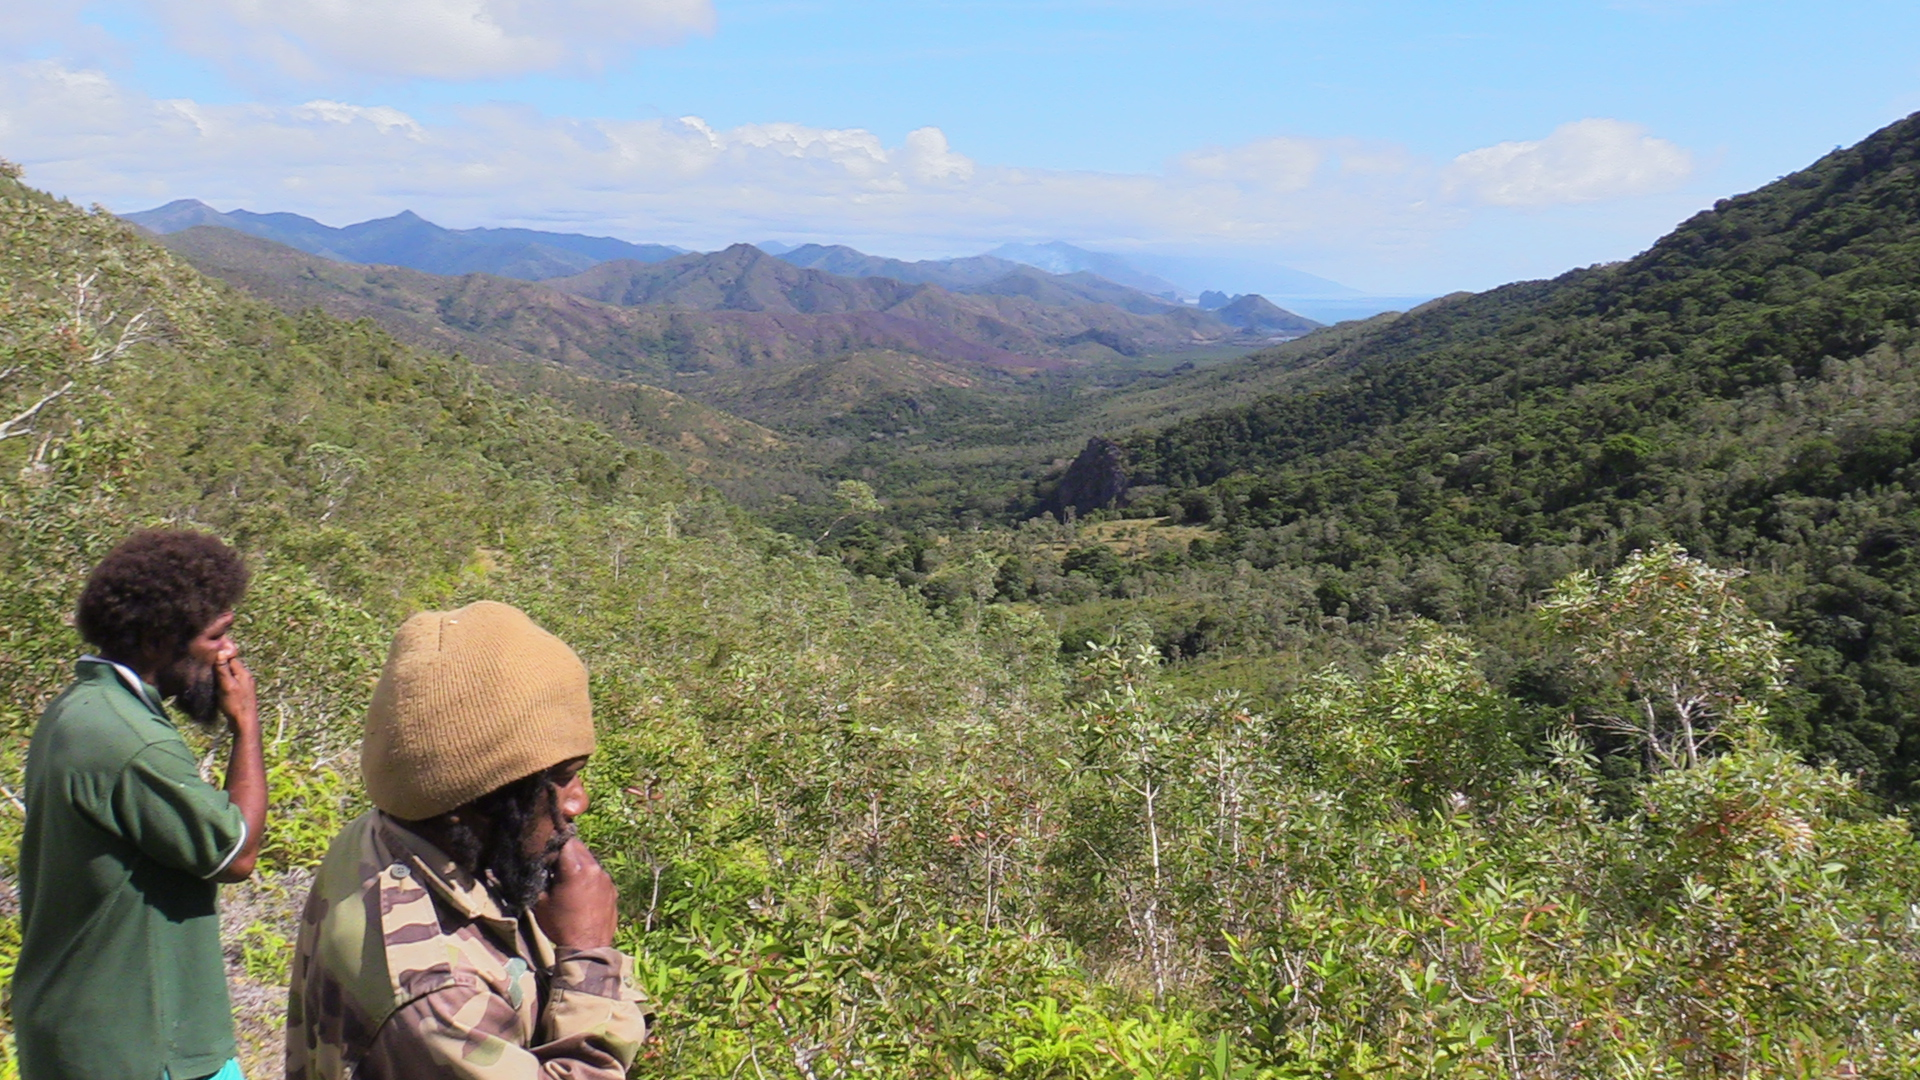
\includegraphics[width=\linewidth]{figures/koin}
	\caption{Mr. Pei and Mr. Kalène looking across the Gaheny creek unto Wanaa. Thehwaade is in the distance, and Seejanit in the blue mists beyond that.}
\end{figure}
 

\appendix
% Appendix B
\chapter{The Rat, the Swamp Hen, and the Squid (Philippe Gohoupe)}
\label{text:squid2}
This story is known all over New Caledonia, and originally from Tiga in the Loyalty Islands. The underlying information of this story, that squids hate rats, and that rats make excellent bait to catch squids, is known beyond the New Caledonian archipelago.\largerpage[2]

\ea%<Hc2-1>

%%\langinfo{}{}{} koin hupwan maa hmasut xahut ka cahma i khîî ahan moo kon maa
\gll Koin hut pwa-n maa a=hma-sut xahut ka cahma i=khîî a=han moo ko-n maa\\ 
end go.down on-\gl{nspec} reef 3\gl{sg}=arrive-go.down below \gl{cnj} \gl{top} \gl{def}.\gl{sg}=swamp.hen \gl{3}\gl{sg}=go stay on-\gl{nspec} reef\\ 
\glt \qu{When the receding tide was low, the Swamp Hen went to stay on the reef [to fish]}

\z
\ea%<Hc2-2>

%%\langinfo{}{}{} ka cahma i siimbwi kon moo cai wâng
\gll ka cahma i=siibwi koon moo ca i=wang\\ 
\gl{cnj} \gl{top} \gl{def}.\gl{sg}=rat \gl{prog} stay in \gl{def}.\gl{sg}=boat\\ 
\glt \qu{and the Rat stayed in the boat.}

\z
\ea%<Hc2-3>

%\langinfo{}{}{} ca i wângalu, a lu vwa wângalu
\gll Ca i=wanga-lu a= lu=vwa wanga-lu
\\ in \gl{def}.\gl{sg}=boat-\gl{3}\gl{du}.\gl{poss} \gl{rel}= \gl{3}\gl{du}=do boat-\gl{3}\gl{du}.\gl{poss}
\\ \glt \qu{In their boat that they made for themselves...}

\z
\ea%<Hc2-4>

%\langinfo{}{}{} ko i ujep. ma moo ka i siibwi a xhuti
\gll Ko i=ujep ma a=moo ka=i=siibwi a xhuti\\ 
\gl{obl} \gl{def}.\gl{sg}=sugar.cane \gl{subr} 3\gl{sg}=stay \gl{sbj}=\gl{def}.\gl{sg}=rat \gl{3}\gl{sg}=scrunch.(sugarcane)\\ 
\glt \qu{...from sugar cane. When the Rat stayed like this, it ate it.}
\z

\ea%<Hc2-5>
%\langinfo{}{}{} cama hamwame ka khîî ma a hmacamwame, paa cika mwa wâng
\gll Cama han-mwa-me ka=khîî, ma=a=hma-ca-mwa-me paa cika mwa wang\\ 
when go-\gl{rep}-\gl{dir.cp} \gl{sbj}=swamp.hen when=\gl{3}\gl{sg}=arrive-go.up-\gl{rep}-\gl{dir.cp} \gl{prf} \gl{neg}.\gl{exist} \gl{rep} boat\\ 
\glt \qu{When Swamp Hen came back, when she came back, the boat was already gone.}

\z
\ea%<Hc2-6>

%\langinfo{}{}{} uwang sin ujep wang-lu ma siibwi pa xhuti meka na siibwi
\gll I=wang sin ujep wang lu ma siibwi paa xhuti meekan a siibwi\\ \gl{def}.\gl{sg}=boat arm sugar.cane boat \gl{3}\gl{du} \gl{subr} rat \gl{pfv} scrunch.(sugarcane) all \gl{sbj} rat\\ \glt \qu{The boat [of] sugar cane branches, their boat, but Rat had already eaten everything.}

\z
\ea%<Hc2-7>

%\langinfo{}{}{} amwa fajimwa ka vi hapi
\gll A=mwa fwajimwake ka vi hapi
\\ 3\gl{sg}=\gl{deict} ask and say \gl{comp}
\\ \glt \qu{She asked him and he said that...}

\z
\ea%<Hc2-8>

%\langinfo{}{}{} a moo a hmanan a paa xhuti
\gll A=moo a=hmana-n a=paa xhuti\\ 
\gl{3}\gl{sg}=stay \gl{3}\gl{sg}=hungry-3\gl{sg} \gl{3}\gl{sg}=\gl{prf} scrunch.(sugarcane)\\ 
\glt \qu{...he stayed, he was hungry, and he ate...}

\z
\ea%<Hc2-9>

%\langinfo{}{}{} xhuti i wâng
\gll xhuti i=wang\\ 
scrunch.(sugarcane) \gl{def}.\gl{sg}=boat\\ 
\glt \qu{...ate the boat.}

\z
\ea%<Hc2-10>

%\langinfo{}{}{} go a vi nyakon a khîî
\gll Go a=vi nyakoo-n a=khîî\\ 
\gl{disc} \gl{3}\gl{sg}=say for-3\gl{sg}.\gl{poss} \gl{sbj}=swamp.hen\\
 \glt \qu{Then Swamp Hen told him:}

\z
\ea%<Hc2-11>

%\langinfo{}{}{} bwa evaang go go cika ca=hun-ta-mwa ko yo vwa li=vuun sung
\gll Bwa e-vaang go go cika eca=hun-ta-mwa ko yo vwa li=vwun s-ung\\ \gl{ipfv} \gl{mid}-unknown \gl{2}\gl{sg} \gl{2}\gl{sg} \gl{neg}.\gl{exist} \gl{indf}.\gl{sg}=\gl{nmlz}-move.up-\gl{rep} because \gl{1}\gl{sg} do \gl{def}.\gl{pl}=hair arm-1\gl{sg}.\gl{poss}\\ \glt \qu{``Well I don't know about you, you don't have any means to go back up, whereas I have my wings."}

\z
\ea%<Hc2-12>

%\langinfo{}{}{} go tha ja tamwame
\gll Go tha a=ja ta-mwa-me\\ then \gl{ass} 3\gl{sg}=\gl{prf} move.up-\gl{rep}-\gl{dir.cp}\\ \glt \qu{And she went back up to the land.}

\z
\ea%<Hc2-13>

%\langinfo{}{}{} ya tha ja thêên thên tamwame
\gll Ya tha ja thêên thêên ta-mwa-me\\ 3\gl{sg} \gl{ass} \gl{prf} run run move.up-\gl{rep}-\gl{dir.cp}\\ \glt \qu{She, she flew up fast to go home.}

\z
\ea%<Hc2-14>

%\langinfo{}{}{} cama i siibwi a balan tabo kon se
\gll Cama i=siibwi a=balan tabo koon se\\ if \gl{def}.\gl{sg}=rat \gl{3}\gl{sg}=finally sit \gl{prog} cry\\ \glt \qu{But the Rat, he just sat there crying.}

\z
\ea%<Hc2-15>

%\langinfo{}{}{} ko i vai a foovwat kon tabo xahut pwan bwanma
\gll Ko i=vai a= fovwat koon tabo xahut pwan bwan-maa\\ on \gl{def}.\gl{sg}=stone \gl{rel}= white \gl{prog} sit below on top-reef\\ \glt \qu{on the white [coral] rock, he was sitting down there on the reef.}

\z
\ea%<Hc2-16>

%\langinfo{}{}{} koin a kon a bwa tena ka i ibwen
\gll Koin a=kon a=bwa tena-a ka i=ibwen\\ stop \gl{3}\gl{sg}=\gl{prog} \gl{3}\gl{sg}=\gl{ipfv} hear-3\gl{sg}.\gl{obj} \gl{sbj} \gl{def}.\gl{sg}=squid\\ \glt \qu{Then he was - the Squid heard him.}

\z
\ea%<Hc2-17>

%\langinfo{}{}{} go a hame a hmacame koon a mwa fajimwa go kon se ko hmwaeke
\gll Go a=hame a=hma-ca-me koo-n a=mwa fwajimwa ``go=kon se ko hmwaeke?"\\ 2\gl{sg} 3\gl{sg}=come 3\gl{sg}=arrive-go.up-\gl{dir.cp} because-\gl{psm} \gl{3}\gl{sg}=\gl{deict} ask 2\gl{sg}=\gl{prog} cry because how\\ \glt \qu{Then he came he came there to him, he was like ``why do you cry?"}

\z
\ea%<Hc2-18>

%\langinfo{}{}{} kavi hapi a se-a moo a=hmanong
\gll Ka a=vi hapi a=se-a moo a=hman-ong\\ and 3\gl{sg}=say \gl{comp} 3\gl{sg}=one-\gl{3}\gl{sg} stay \gl{3}\gl{sg}=hungry-\gl{1}\gl{sg}.\gl{poss}\\ \glt \qu{And he said that he was alone and ``I was hungry".}

\z
\ea%<Hc2-19>

%\langinfo{}{}{} a xhuti wâng aju
\gll A=xhuti i=wanga-ju\\ \gl{3}\gl{sg}=scrunch.(sugarcane) \gl{def}.\gl{sg}=boat.\gl{poss}-3\gl{du}.\gl{poss}\\ \glt \qu{He ate our boat.}

\z
\ea%<Hc2-20>

%\langinfo{}{}{} paa ja pa cika mwa ca=wang-abu m=abu taa-mwa kabu 
\gll Paa ja paa cika mwa ca=wang-abu m=abu ta-mwa ka=bu\\ \gl{pfv} \gl{prf} \gl{pfv} \gl{neg}.\gl{exist} \gl{rep} \gl{indf}.\gl{sg}=boat-\gl{1}\gl{du}.\gl{excl} \gl{subr}=\gl{1}\gl{du}.\gl{excl} move.up-\gl{rep} \gl{sbj}=1\gl{du}.\gl{excl}\\ \glt \qu{And now there is no more, no more boat of ours with which we could go back up.}
\z

\ea%<Hc2-21>
%\langinfo{}{}{} go ya avi hapi go tha vaang go yo theja thêên tamwa ko vwa li=vuun sung
\gll  Go ya a=vi hapi go tha vaang go yo thêên tamwa ko vwa li=vwun s-ung\\  \gl{disc} \gl{3}\gl{sg} \gl{3}\gl{sg}=say \gl{comp} \gl{2}\gl{sg} \gl{ass} inconnu \gl{2}\gl{sg} \gl{1}\gl{sg} run go.back.up because \gl{exist} \gl{def}.\gl{pl}=hair arm-1\gl{sg}.\gl{poss}\\ \glt \qu{And she said “I don't know about you, I'm leaving because I have wings."}
\z

\ea%<Hc2-22>
%\langinfo{}{}{} ko camwa siibwi ko tabo kon se se se a tena ka ibwen a hame
\gll Ko cahma siibwi koon tabo koon se se se a=tena ka ibwen a=ha-me\\ \gl{cnj} \gl{top} rat \gl{prog} sit \gl{prog} cry cry cry \gl{3}\gl{sg}=hear \gl{sbj} squid \gl{3}\gl{sg}=go-\gl{dir.cp}\\ \glt \qu{And Rat, he sits, he cries, cries, cries, Squid hears and comes.}

\z
\ea%<Hc2-23>

%\langinfo{}{}{} a fajimwa ha go siibwi go se se ko hmwaeke
\gll A=fwajimwake ha go siibwi go=se se ko hmwaeke\\ \gl{3}\gl{sg}=ask \gl{expl} \gl{2}\gl{sg} rat \gl{2}\gl{sg}=cry cry \gl{obl} how\\ \glt \qu{He asks ``Hey you, Rat, why do you cry, cry?"}
\z

\ea%<Hc2-24>
%\langinfo{}{}{} e=se ko e=xhuti i wangabe, abe hupwe ma khîî kon ya tha paa tamwa
\gll E=se ko e=xhuti i=wang-abe abe=hup-e ma khîî kon ya tha paa ta-mwa\\ \gl{1}\gl{sg}=cry because 1\gl{sg}=scrunch.(sugarcane) \gl{def}.\gl{sg}=boat-\gl{1}\gl{pl}.\gl{excl}.\gl{poss}\gl{1}\gl{pl}.\gl{excl}=go.down-\gl{dir.cp} \gl{subr} swamp.hen \gl{cnj} \gl{3}\gl{sg} \gl{ass} \gl{prf} go.up-\gl{rep}\\ \glt \qu{``I cry because I ate our boat, we came down with Swamp Hen, and she already went back up."}

\z
\ea%<Hc2-25>
%\langinfo{}{}{} go ka go hame ko e=bo fetamwako
\gll Go ka go=ha-me ko e=bo fe-ta-mwa-ko\\ \gl{2}\gl{sg} \gl{sbj} \gl{2}\gl{sg}=go-\gl{dir.cp} because \gl{1}\gl{sg}=\gl{irr} take-move.up \gl{rep}-2\gl{sg}\\ \glt \qu{``You, come, because I will take you back up."}

\z
\ea%<Hc2-26>

%\langinfo{}{}{} hê a ja han tabo pwan bwan kona ja fetamwamea
\gll Hê a=ja han tabo pwa-n bwa-n kona a=ja fe-ta-mwa-me-a\\ yes \gl{3}\gl{sg}=\gl{prf} go sit on-\gl{nspec} head-3\gl{sg}.\gl{poss} \gl{cnj} 3\gl{sg}=\gl{prf} take-move.up-\gl{rep}-\gl{dir.cp}-\gl{3}\gl{sg}.\gl{obj}\\ \glt \qu{Yes, he goes to sit on his head and he takes him back up.}

\z
\ea%<Hc2-27>

%\langinfo{}{}{} lu hmacamwame can hmeewan
\gll Lu=hma-ca-mwa-me ca-n hmeewan\\ \gl{3}\gl{du}=arrive-go.up-\gl{rep}-\gl{dir.cp} on-\gl{nspec} sand\\ \glt \qu{The two arrive up at the beach,}

\z
\ea%<Hc2-28>

%\langinfo{}{}{} ma xhasat nyadamwa siibwi phâêû
\gll Ma xhasaat nya-da-mwa siibwi phâêû\\ \gl{subr} jump towards-up-\gl{deict} rat dry.land\\ \glt \qu{so that Rat [can] jump up back onto dry land.}

\z
\ea%<Hc2-29>

%\langinfo{}{}{} go cahma i ibwen a ja hupwa a konja hupwale can we
\gll Go cahma i=ibwen a=ja hut a=koon ja hup-wa-le ca-n we\\ \gl{2}\gl{sg} \gl{top} \gl{def}.\gl{sg}=squid \gl{3}\gl{sg}=\gl{prf} move.down \gl{3}\gl{sg}=\gl{prog} \gl{prf} go.down-\gl{rep}-\gl{dir.cf} in-\gl{nspec} water\\ \glt \qu{And the Squid, he goes back down, he is going back away into the water.}
\z
\pagebreak
\ea%<Hc2-30>

%\langinfo{}{}{} a cuut mwa ka siibwi a emwadia a emwadia a mwadike mwa i ape xhwata can bwan
\gll A=cuut mwa ka siibwi mwa a=e-mwadi-a a=e-mwadi-a a=mwadi-ke i=ape-xhwata ca-n bwa-n\\ \gl{3}\gl{sg}=stand \gl{deict} \gl{sbj} rat \gl{deict} 3\gl{sg}=\gl{refl}-laugh-3\gl{sg}.\gl{obj} 3\gl{sg}=\gl{refl}-laugh-3\gl{sg}.\gl{obj} 3\gl{sg}=-laugh-\gl{tr} \gl{def}.\gl{sg}=\gl{loc}.\gl{nmlz}-bald in-\gl{nspec} head-3\gl{sg}.\gl{poss}\\ \glt \qu{Rat stands now and laughs to himself, laughs about the bald spot on his head.}

\z
\ea%<Hc2-31>

%\langinfo{}{}{} ibwan ibwen a xhwata
\gll I=bwa-n ibwen a= xhwata\\ 
\gl{def}.\gl{sg}=head-\gl{nspec} squid \gl{rel}= bald\\ 
\glt \qu{The bald squid head.}

\z
\ea%<Hc2-32>

%\langinfo{}{}{} aemwadia kona tena ka i ibwen
\gll A=e-mwadi-a kona a-tena-a ka i=ibwen\\ 3\gl{sg}=\gl{refl}-laugh-3\gl{sg}.\gl{obj} then hear \gl{sbj} \gl{def}.\gl{sg}=squid\\ \glt \qu{He laughed to himself, then he was heard by the Squid.}

\z
\ea%<Hc2-33>

%\langinfo{}{}{} ha go go mwadike i da?
\gll Ha go go=mwadi-ke i=da\\ 
\gl{expl} \gl{2}\gl{sg} \gl{2}\gl{sg}=laugh-\gl{tr} \gl{def}.\gl{sg}=what\\ 
\glt \qu{``Hey you! What are you laughing about?"}

\z
\ea%<Hc2-34>

%\langinfo{}{}{} e=mwadike xhwatakam
\gll E=mwadi-ke xhwata ka-m\\ 
\gl{1}\gl{sg}=laugh-\gl{tr} bald \gl{clf}.\gl{poss}-\gl{2}\gl{sg}.\gl{poss}\\ 
\glt \qu{``I laugh of your baldness."}
\z
\ea%<Hc2-35>

%\langinfo{}{}{} go go thuang-o ta-me na yo efetame-ko can! 
\gll Go go=thuang-o ta-me na yo e=fe-ta-me-ko can, \\ \gl{2}\gl{sg} \gl{2}\gl{sg}=joke-\gl{1}\gl{sg}.\gl{obj} move.up-\gl{dir.cp} \gl{dem} \gl{1}\gl{sg} 1\gl{sg}=take-move.up-\gl{dir.cp}-2\gl{sg}.\gl{obj} in\\ \glt \qu{``You, you laugh of me walking up [to dry land], it is me who brought you up here!"}

\z

\ea

%\langinfo{}{}{} a thake nyadame i thaangan kona thaakea
\gll A=thake nya-da-me i=thaangan koo-n a=thake-a\\  \gl{3}\gl{sg}=throw send-go.up-\gl{dir.cp} \gl{def}.\gl{sg}=tentacle on-3\gl{sg} \gl{3}\gl{sg}=throw-\gl{3}\gl{sg}.\gl{obj}\\ \glt \qu{Then he threw his tentacle and then hit him.}
\z
\pagebreak

\ea%<Hc2-36>
%\langinfo{}{}{} thakea thakea hut can we go a yabilo-a
\gll Thake-a thake-a hut ca-n we go a=yabilo-a\\ throw-\gl{3}\gl{sg}.\gl{obj} throw-\gl{3}\gl{sg}.\gl{obj} move.down in water then \gl{3}\gl{sg}=kill-3\gl{sg}.\gl{obj}\\ 
\glt \qu{Threw him, threw him down into the water, then he killed him.}
\z
\ea%<Hc2-37>

%\langinfo{}{}{} go ethuago e=nyauko can we ma bup nyanaam 
\gll Go=e-thuang-o e=nya-ut-ko ca-n we ma bup hnyanaa-m\\ \gl{2}\gl{sg}=\gl{refl}-joke-\gl{1}\gl{sg}.\gl{obj} \gl{1}\gl{sg}=put-go.down-2\gl{sg}.\gl{obl} in-\gl{nspec} water \gl{subr} thunder.strike breath-\gl{2}\gl{sg}.\gl{poss}\\ \glt \qu{``You laugh about me, I'll drag you down into the water to burst your breath."}

\z
\ea%<Hc2-38>

%\langinfo{}{}{} go aja vwa mwa mekai siibwi
\gll Go a=ja vwa ma me ka=i=siibwi\\ 
then \gl{3}\gl{sg}=\gl{prf} do \gl{subr} die \gl{sbj}=\gl{def}.\gl{sg}=rat\\ 
\glt \qu{And he made the Rat die.}

\z
\ea%<Hc2-39>

%\langinfo{}{}{} cahma ibwen thaja hupwa
\gll Cahma ibwen tha ja hup-wa\\ \gl{top} squid \gl{ass} \gl{prf} go.down-\gl{rep}\\ \glt \qu{And the Squid, it went back down.}

\z
\ea%<Hc2-40>

%\langinfo{}{}{} thaja koin mwa siibwi thapa mea thapaja seada
\gll Tha ja koin mwa siibwi tha pa me-a tha=a=pa ja sea-da\\ \gl{ass} \gl{prf} stop \gl{rep} rat \gl{ass} already die-\gl{3}\gl{sg}.\gl{obj} \gl{ass}=3\gl{sg}=\gl{pfv} \gl{prf} look-go.up\\ \glt \qu{This is the end now, Rat is dead, he looks upwards now.}

\z



\chapter{The 1917 Tipije War (Philippe Gohoupe)}
\label{text:tipije}
%\usepackage{glossingtool}
%\label{Appendixme} % Change X to a consecutive letter; for referencing this appendix elsewhere, use \ref{AppendixX}
%\begin{document}
%\maketitle
%\glossingAbbrevsList

%%todo{is \textit{thathe} in \ref{ex:thathe1} vs \ref{ex:thathe2} active vs passive in meaning?}

This is a version of what happened in the Tipije valley as Mr. Gohoupe's parents experienced it. The storytelling lapses back and forth at certain moments, and most of the participants are not formally introduced. This is due, apart from Mr. Gohoupe's age, to the audience: they all grew up in the area and know the story. Briefly summarized, first Kafeyat Cidopwaan, chief of Ouen Kout/Wan Kuut, was blamed for the attacks on settler households (see \chapref{chap:Tipije}), and when the European soldiers stationed in Dewanwe conducted punitive expeditions, he was shot in the back near Tendo; he died in a creek there. All men were assembled and either killed in the process or sent to Nouméa to be questioned. The women were sent to Houaïlou. At the same time, the colonial authorities looked for the chiefs responsible for the war, and as the mother of chief Kafeyat could show a black shell money, used to broker war alliances, and as she said that the chief of Hienghène, Bwaarat, had sent it to call his allies to war, the blame shifted onto Bwaarat. He hanged himself when he heard that a ship had come to take him to the guillotine. The men and women were then released from prison.\largerpage[2]

\section{Introduction} 

Asked by Nigai Kalène:

 \ea 
\gll A=kon vi hapi na gasu=\textit{enregistrer} koin gase=bo=pala\\ 
3\gl{sg}=\gl{prog} say that \gl{dem} 1\gl{du}.\gl{incl}=record finish 1\gl{pl}.\gl{incl}=\gl{irr}=say \\ \glt  \qu{‎‎He is saying that we two will [press] record, then we all will talk.}
\z 

\ea
\gll Hêê da... cama nyima-m ma go=\textit{enregistrer} ce-ma go=bo pala ma bo fainake koin cama nyima-m ma go=xaahni ma i=e-vwa-kan nyakoo-m.\\ 
yes what if/\gl{irr} will-2\gl{sg}.\gl{poss} \gl{subr} 2\gl{sg}=record if/\gl{irr} 2\gl{sg}=\gl{irr} speak \gl{subr} \gl{irr} show finish if will-2\gl{sg}.\gl{poss} \gl{subr} 2\gl{sg}=keep with \gl{def}.\gl{sg}=\gl{nmlz}.\gl{ins}-do-\gl{nmlz} for-2\gl{sg}.\gl{poss}\\ 
\glt \qu{Yes, uh, if you want to record, when you will talk to explain, then you can keep it as a tool for yourself.} 
\z 

\ea
\gll ma xaani nyakoo... ya a=vi canbwen \\ 
\gl{subr} keep for 3\gl{sg} 3\gl{sg}=say yesterday \\ 
\glt \qu{And keep for... he said it yesterday.}
 \z 

\ea
 %cama goon eca aman?
\gll Evwakan nyako li=mwa-n-somun gase=bo=bwaa=pala koon cama goon ca aman... thapoke fwajimwake \\ 
tool for \gl{def}.\gl{pl}=house-\gl{link}-lesson 1\gl{pl}.\gl{incl}=\gl{irr}=\gl{ipfv}=speak \gl{obl}-3\gl{sg} if enough in? something begin ask \\ 
 \glt \qu{Preserve it for the schools, we'll talk about it. If we may, something... start asking.}
\z 

\ea
\gll E-nyima-n ma caihna-n i=hun-moo-kan cala le=fe ka=li=popwaale ce veandan vwa vaa. hê ko i=va.\\ 
\gl{refl}-will-3\gl{sg}.\gl{poss} \gl{subr} know-\gl{nspec} \gl{def}.\gl{sg}=\gl{nmlz}-stay-\gl{nmlz} when.\gl{real} 3\gl{pl}=fetch \gl{sbj}=\gl{def}.\gl{pl}=European in time \gl{exist} war yes about \gl{def}.\gl{sg}=war\\ 
 \glt \qu{He wants to know about the time when they were taken by the Europeans, in the time when there was a war. Yes, about the war.} 
\z

\section{Story}% (Philippe Dego Gohupe $\sim$ 80 years old):

\ea
\gll Kona li=pupwaale tha le=pa fe cahni ko-nya seen hnya hnut-te\\ 
well \gl{def}.\gl{pl}=European \gl{ass} 3\gl{pl}=\gl{prf} take here on-toward border toward downstream-\gl{dir.cf}\\ 
\glt \qu{The Europeans had taken it, here until the border towards down there.}
 \z
  
\ea
\gll Le=hmasa-me ka li=pupwaale kon cahni li=apuli li=xhaohmu moo seen xahnut ca-n la la li=xhwaapwê\\ 
3\gl{pl}=arrive-\gl{dir.cp} \gl{sbj} \gl{def}.\gl{pl}-Europeans \gl{cnj}? here \gl{def}.\gl{pl}=person \gl{def}.\gl{pl}=elder stay border downstream in-\gl{ana} here here \gl{def}.\gl{pl}=colonnary.pine\\ 
\glt \qu{The Europeans came, and here the people, the ancestors stayed, till the border down there here where the araucaria pines are.}
\z 

\ea
\gll Kone le=hma wati-le nya cahni hma xaa-le le=thapoke cahni na tha i=seen nya-an-de \\ 
when 3\gl{pl}=arrive chase-3\gl{pl} from here until\footnotemark hit-3\gl{pl} 3\gl{pl}=begin here \gl{dem} \gl{ass} \gl{def}.\gl{sg}=border further-go-\gl{dir.cf} \\ 
\glt \qu{When they arrived here while chasing them, they began here and this is the limit [of their movement] over there (visible).}
\ex
\gll Li=apuli li=xhaohmu kona... li=pupwaale kona... tha i=seen hnya hnut-te\\ \gl{def}.\gl{pl}=person \gl{def}.\gl{pl}=elder and? \gl{def}.\gl{pl}=European and? \gl{ass} \gl{def}.\gl{sg}=border towards downstream-\gl{dir.cf}\\ \glt \qu{The people, the ancestors, well... the Europeans, well... this is the border down there.}
\ex\largerpage[2]
\gll Koin le=hma wati-le ma xaa-le hnuuda-me cahni\\ 
then 3\gl{pl}=arrive chase-3\gl{obj} \gl{subr} beat-3\gl{obj} upstream-\gl{dir.cp} here\\ 
\glt \qu{Then they came chasing them to strike them, coming up here.}
\ex
\gll Koin le=bwa hân hân cop xada koin le=hup-wa xahan xahut le seejanit \\ % koin le bwa-da ha thê\\ 
while 3\gl{pl}=\gl{ipfv} go go go.over up.there finish 3\gl{pl}=go.down-\gl{rep} over.there down.there 3\gl{pl} T. \\%finish %3\gl{pl} \gl{ipfv}-? go? rock
\glt \qu{Then they [the Kanak] went from there and walked, walked, crossed [the mountain] up there and then went back down over there, they were in Tiendanite.} 
\ex\label{ex:thathe1}
\gll Bwa xada thathee mwa maahma ca i=dingan xahan thêêdo\\ \gl{ipfv} up.there kill \gl{rep} elder.brother in \gl{def}.\gl{sg}=creek over.there T.\\ \glt \qu{Up there was killed the chief [Kafeyat Cidopwaan of Wan Kuut], in the creek over there in Tendo.}
\ex
\gll Go le=fwade-a nya-mwa-la ko ya mwa si-n i=mwa-n hmat ko i=vaa a=hnyada-me ka=thêama \\ then 3\gl{pl}=seek.\gl{anim} towards-\gl{rep}-\gl{prox} because 3\gl{sg} \gl{deict} \gl{ben}-3\gl{sg}\gl{poss} \gl{def}.\gl{sg}=container-\gl{poss} customary.money for \gl{sg}.\gl{def}=war 3\gl{sg}=send-\gl{dir.cp} \gl{sbj}=chief \\ \glt  \qu{Well, they looked for him around that time, because it was him now, to him that the great chief [Bwarhat of Hienghène] had sent the war money.}
\z 
\footnotetext{lit. \qu{until}}
\ea

\gll I=se mwa-n solda a=moo xahnut pwanvai ka i=se a=moo xahut dewanwe \\ 
\gl{def}.\gl{sg}=other house-\gl{poss} soldier 3\gl{sg}=stay downstream.there P. \gl{cntr} \gl{def}.\gl{sg}=other 3\gl{sg}=stay down.there T.\\
 \glt \qu{One barracks was in Pwanvai and one in Dewanwe [the coast of Tiouandé].}
\z 

\ea
\gll Cipa gase=va caihnan mwa nya la hun-moo ka i=vaa \\
\gl{neg} 1\gl{pl}.\gl{incl}=strongly know \gl{rep} put here \gl{nmlz}-stay \gl{link} \gl{def}.\gl{sg}=war\\ 
\glt \qu{We don't know too well anymore what put the war here.}
\z 

\ea
\gll Ko na a=nyadaa-me ka bwaaxat tha i=hmat-aen \\ but \gl{dem} 3\gl{sg}=send-\gl{dir.cp} \gl{sbj} B. \gl{ass} \gl{def}.\gl{sg}=customary.money-\gl{dem} \\ \glt \qu{But that which Bwaaxat sent, was that [war] shell money.}
 \z 
 
 \ea\label{ex:thathe2}
\gll Go le=ja thathe-a mwa go le=nya siwa-mwa\\ \gl{disc} 3\gl{pl}=\gl{prf} kill-3\gl{pl} \gl{rep} then 3\gl{pl}=send return-\gl{rep}\\ \glt \qu{And they had already slayed him then, and [the women and tribespeople] went back (home).}
 \z 

\ea
\gll Cama hma-ca-me ka i=mwa-n hmat ka lu=tua lu ma ya lu ma\\ when arrive-go.up-\gl{dir.cp} \gl{sbj} \gl{def}.\gl{sg}=container-\gl{poss} customary.money \gl{cntr} 3\gl{du}=take.out 3\gl{du} \gl{com} 3\gl{sg} 3\gl{du} \gl{com}\\ \glt \qu{When the shell money arrived, the two [mothers took] it out.}% elle et l'autre}
\z 

\ea
\gll A=vi maman Henri ma mama-le mwa lu=tua a=fe i=dipi ka i=see koin a=fe i=sanan ka i=see \\ 3\gl{sg}=say mother H. \gl{com} mother-3\gl{pl}\gl{poss} \gl{rep} 3\gl{du}=take.out 3\gl{sg}=take \gl{def}.\gl{sg}=cover \gl{sbj} \gl{def}.\gl{sg}=other while 3\gl{sg}=take \gl{def}.\gl{sg}=content \gl{sbj} \gl{def}.\gl{sg}=other \\ \glt  \qu{‎‎That means Henri's mother and the mother of the others, the two took [the shell money] out and one took the wrap, then the other took the content.}
\z 

\ea\label{ex:thathe3}
\gll Ma le=han ma ja han thathe-a mwa kon le=ja siwa-mwa \\ \gl{subr} 3\gl{pl}=go \gl{subr} \gl{prf} go kill-3\gl{sg} \gl{rep} then 3\gl{pl}=\gl{prf} return-\gl{rep}\\ \glt \qu{When [the mothers] fled, when he had died, then [the survivors] returned.}
\z 

\ea
\gll Ma le=ja hmaca-mwa Noumea le=ja fee-le mwa jevwan mwa acan ka li=xhaomu mwa le=moo cahni \\ \gl{irr} 3\gl{pl}=\gl{prf} arrive-\gl{rep} N. 3\gl{pl}=\gl{prf} take-3\gl{pl} \gl{deict} l'ensemble \gl{rep} among \gl{sbj} \gl{def}.\gl{pl}=elder \gl{rep} 3\gl{pl}=stay here\\ \glt \qu{When they arrived in Noumea, they took them then, the whole lot, among them the ancestors as well who lived here.}
\z 

\ea
\gll Acan ka i=hao-nea tha u vwa mwa li=been\\ among \gl{sbj} \gl{def}.\gl{sg}=grandfather-3\gl{sg}.\gl{poss} \gl{ass} ? \gl{exist} also \gl{def}.\gl{pl}=brothers\\ \glt \qu{Among them was the [chief's] grandfather, there were also the others.}
\z 

\ea
\gll Na cahni tha xhwan see-a a thathe-a cahni. \\ \gl{dem} here \gl{ass} a.bit one-3\gl{sg} \gl{rel} kill-3\gl{sg} here\\ \glt \qu{Here, there was only one who was slain.}
\z 

\ea
\gll I=a thathe-a na i=bee i=papa-n ena xahnuut pwanbaut mwa\\  \gl{def}.\gl{sg}=\gl{rel} kill-3\gl{sg} \gl{dem} \gl{def}.\gl{sg}=brother \gl{def}.\gl{sg}=father-\gl{poss} \gl{dist} downstream P. \gl{rep}\\ \glt \qu{He who was killed was the brother of the father of those downstream in Pwanbaut there.}
\z

\ea
\gll Kavi i=bee-n i=papa-n-le yata-n bwaungan\\ 
but \gl{def}.\gl{sg}=brother-\gl{poss} \gl{def}.\gl{sg}=father-3\gl{pl}\gl{poss} name-3\gl{pl}\gl{poss} B.\\ 
\glt \qu{By the way, their father's brother's name was Bwaungan.}
\z 

\ea
\gll Thathe-a nya xahan waneut ma le=siwa-mwa \\ 
kill-3\gl{sg} \gl{prox} over.there O.-K. \gl{irr}? 3\gl{pl}=return-\gl{rep}  \\ 
\glt \qu{He died all the way over there in Ouen Kout when they came back.}
\z


\ea
\gll Ka le=ja fwadai-mwa ka li=pupwaale a=ja ha thaloot ka bwaaxat a=e-vwa-koo-n ka bwaaxat li=apuli-nea\\ \gl{cntr} 3\gl{pl}=\gl{prf} find.\gl{inan}-\gl{rep} \gl{sbj} \gl{def}.\gl{pl}=European 3\gl{sg}=\gl{prf} ? come.out \gl{sbj} B. 3\gl{sg}=\gl{refl}-do-\gl{obl}-3\gl{sg} \gl{sbj} B. \gl{def}.\gl{pl}=man-3\gl{sg}.\gl{poss}
\\ \glt \qu{The Europeans were looking for [the reason] and Bwaarat emerged. It turned out it was Bwaarat and his men.}
\z

\section{Death of Bwaxat}

\ea
\gll Fe-ta ma le=hup-e thai-le ma le=ta mwa-n suki aman\\ take-go.up \gl{subr} 3\gl{pl}=go.down-\gl{dir.cp}? attach-3\gl{pl} \gl{subr} 3\gl{pl}=go.up house-\gl{poss} pay something\\ \glt \qu{Brought up to come down and gather them so that they would go up to prison}
\z 

\ea
\gll Hê fwandai ca=wuukin, hapi na wukin Bwaxat. \\ 
yes seek.\gl{inan} some=reason \gl{comp} \gl{dem} reason B. \\ \glt \qu{Yes, looked for some reason [for the war], that it was Bwaarat's fault.} 
\z 

\ea
\gll Xhu-pwa-mee i=wang le=bwa vii hapi na ``ya ya thapoke i=vaa"\\ go.down-\gl{rep}-\gl{dir.cp} \gl{def}.\gl{sg}=boat 3\gl{pl}=\gl{ipfv} say that \gl{dem} 3\gl{sg} 3\gl{sg} begin \gl{def}.\gl{sg}=war\\ \glt \qu{The boat came down. They said that ``he, he started the war".}
\z

\ea
\gll A=ja hu-pwa-mee umwang, hu-pwa-me fe-a, ce i=wadan thangavi nyôô-n apuli\\ 3\gl{sg}=\gl{prf} go.down-\gl{rep}-\gl{dir.cp} boat go.down-\gl{rep}-\gl{dir.cp} take-3\gl{sg} in \gl{def}.\gl{sg}=time chop neck-\gl{poss} person\\ \glt \qu{The boat came down, came down north to take him, in the time when they would cut people's necks.}
\z \ea

\gll Ce i=wadan a=hma-cuut ka i=umwang, ka le=fe-ta, koma le=fe-a, ka i=wang a=ha-me hma-cuut, ya, a=ta wainyô nyece i=juu-mwa\\ in \gl{def}.\gl{sg}=time 3\gl{sg}=arrive-stand \gl{sbj} \gl{def}.\gl{sg}=ship \gl{cntr} 3\gl{pl}=take-go.up-3\gl{sg} in.order.to 3\gl{pl}=take-3\gl{sg} \gl{cntr} \gl{def}.\gl{pl}=boat 3\gl{sg}=go-\gl{dir.cp} arrive-stand 3\gl{sg} 3\gl{sg}=go.up tie.neck in(building) \gl{def}.\gl{sg}=real-house\\ \glt \qu{At this moment when the boat arrived, and they brought it north to catch him, and the boat had arrived at the shore, him, he had hanged himself in the house.}
\z 

\ea
\gll Ma le=ta, ma le=xale-a, ko-ma le=fe-a, ma le=ta ma le=fe-a, ya, a=pa ja me-a ma le=hmasa-mwa xada ma le=ja fwandai ta-mwa
 \\ \gl{com} 3\gl{pl}=go.up \gl{subr} 3\gl{pl}=see-3\gl{sg} because-\gl{subr} 3\gl{pl}=take-3\gl{sg} \gl{com} 3\gl{pl}=go.up \gl{subr} 3\gl{pl}=take-3\gl{sg} 3\gl{sg} 3\gl{sg}=\gl{prf} \gl{prf} die-3\gl{sg} when 3\gl{pl}=arrive-\gl{rep} up.there when 3\gl{pl}=\gl{prf} seek.\gl{inan} go.up-\gl{rep}
 \\ \glt  \qu{When they went up, to see him, to take him, when they went up to take him, him, he was already dead when they arrived up there, when they searched coming back up north.} 
\z 

\section{Black Money and the Return of the People}
 \ea
\gll Go a=ja ta mwa ka i=thamo i=mama-n maama ma\\ then 3\gl{sg}=\gl{prf} go.up \gl{deict} \gl{sbj} \gl{def}.\gl{sg}=woman \gl{def}.\gl{sg}=mother-\gl{poss} chief\footnotemark \gl{subr}\\ \glt \qu{Then she went south, the woman, the mother of the chief [Kafeyat], to...}
\z 
\footnotetext{{lit. \qu{elder brother}}}
\ea
\gll A=fainake i=mwa-n hmat a=nya ka ena na ehni xaaci civije\\ 3\gl{sg}=show \gl{def}.\gl{sg}=container-\gl{poss} customary.money 3\gl{sg}=give \gl{sbj} \gl{dist} \gl{dem} \gl{prox} strike T.\\ \glt \qu{...show the sheath of shell money that he had sent, him who struck Tipije.}
\z 

\ea
\gll Le=ja vatipwe-mwa, kon ya tha pa ja me-a. go, tha le=ja thuat-mwa moo, ka li=xhaomu, ja, tha le=ja ha-mwa-me\\ 3\gl{pl}=\gl{prf} drop-\gl{rep} because 3\gl{sg} \gl{ass} \gl{pfv} \gl{prf} die-3\gl{sg} then \gl{ass} 3\gl{pl}=\gl{prf} emerge-\gl{rep} stay \gl{sbj} \gl{def}.\gl{pl}=elder \gl{prf} \gl{ass} 3\gl{pl}=\gl{prf} go-\gl{rep}-\gl{dir.cp}\\ 
\glt  \qu{They were released, because he was already dead. Well, they came back out [of prison], the ancestors, yeah, they came back.}
\z 

\ea
\gll Go, cahma li=xayu, le=thai-le hnya-da-le wailu\\ 
and concerning \gl{def}.\gl{pl}=male 3\gl{pl}=pick.up-3\gl{pl} send-move.south-3\gl{pl} H.\\ \glt \qu{And, the men, they gathered them and sent them south to Houailou. [this is probably a mistake of the speaker]}
 \z 
 
 \ea
\gll Can goakan-aen, le=hma-cup-wa-me ka li=xayu, ma le=hup-wa-me, ka li=thamo, le=moo wailu \\ in moment-\gl{dem} 3\gl{pl}=arrive-down.there-\gl{rep}-\gl{dir.cp} \gl{sbj} \gl{def}.\gl{pl}=woman \gl{com} 3\gl{pl}=go.down-\gl{rep}-\gl{dir.cp} \gl{sbj} \gl{def}.\gl{pl}=woman 3\gl{pl}=stay H. \\ \glt \qu{At this moment, the men came back, when they came back, and the women, they stayed in Houailou.}
\z 

\ea
\gll A=vi ka Leenhardt hapi i=apuli a=vwa ka i=thamo, go, ya a=fa-thuati i=apuli\\ 3\gl{sg}=say \gl{sbj} L. that \gl{def}.\gl{sg}=man 3\gl{sg}\textsubscript{1}=do \gl{sbj} \gl{def}.\gl{sg}=woman\textsubscript{1} then 3\gl{sg} 3\gl{sg}=\gl{caus}-come.out.\gl{tr} \gl{def}.\gl{sg}=man\\ 
\glt \qu{Leenhardt said that the man is there thanks to the woman, well, he had the man [=the women?] freed.}
\z 

\ea
\gll Nyasi Leenhardt, e=bwa ju tena i=yata-n, cip=e xa-xale-a \\ \gl{top} L. 1\gl{sg}=\gl{ipfv} truly hear \gl{def}.\gl{sg}=name-3\gl{sg}.\gl{poss} \gl{neg}=1\gl{sg} \gl{hab}-see-3\gl{sg}\\ 
\glt \qu{Concerning Leenhardt, I did hear his name, but I never saw him.}
\z

\chapter{The Story of the Dance Beat (Yvonne Sahilé)}

This is a legend written by Yvonne Sahilé, a writer and culture activist living in Tiouandé. She drew on traditional motifs, e.g. the Cannibal of Tipije, the knowledge transmitted by bloodlines (the dance is recognized by the father), and everyday details. Mrs. Sahilé wrote this story in French, and it was translated into Vamale by André Kalen, Jacob Oué and Christophe Pei. Her names for the protagonists are in Pije, and were kept that way in the translations.

\label{text:beat}
\ea %\label{ex:t1}

%\langinfo{}{}{} 1
\gll 	Habu Can-Vije vwa i=apemoo a=pwa-n jela i=jahoot a=xhopwen.	\\	long.ago Tipije \gl{exist} \gl{def}.\gl{sg}=tribe \gl{rel}=on-\gl{nspec} side \gl{def}.\gl{sg}=river \gl{rel}=big	\\ \glt  \qu{Long ago in the Tipije valley, there was a tribe on the bank of this great river.} (following the French original text)		


\z \ea %\label{ex:t2}
%\langinfo{}{}{} 2
\gll 	Ca i=apemoo-ca le=vacuti \textbf{ca} daahma a=bwa xawe ka yata-n Thêa Xa-vila.	\\	in \gl{def}.\gl{sg}=tribe-\gl{prox} 3\gl{pl}=erect some chief \gl{rel}=\gl{ipfv} young and name-3\gl{sg}.\gl{poss} T. \gl{nmlz}-dance	\\ 
\glt  \qu{In this tribe they erected some chief who was still young, and his name was Firstborn the Dancer.}		
\z 

\ea %\label{ex:t3}
%\langinfo{}{}{} 3
\gll Ca \textbf{i}=apemoo vwa \textbf{li}=xawe thamo.
\\ in \gl{def}.\gl{sg}=tribe \gl{exist} \gl{def}.\gl{pl}=young woman	
\\ \glt \qu{In the tribe were young women.} (indefinite, non-specific in the French original)
\z 

\ea %\label{ex:t4-6}
%\langinfo{}{}{} 4,5,6
\gll Tha fe nyamaa-n can dawee-le \textbf{eca} thamo a=en maa-n.\\ 
     \gl{ass}.3\gl{sg} take eye-3\gl{sg}.\gl{poss} in between-3\gl{pl}.\gl{poss} \textbf{some} woman \gl{rel}=first face-3\gl{sg}.\gl{poss}\\ 
\glt \qu{The most beautiful woman between them ``took his eye".}
\z

\ea
\gll Ka a=xhani ma mwada-n. Yata-n In Fwe.\\ 
and 3\gl{sg}=choose \gl{subr} wife-3\gl{sg}.\gl{poss} name-3\gl{sg}.\gl{poss} skin guettarda.speciosa\\ 
\glt \qu{And he chose her as his wife. Her name was Figtree Bark.}
\z

\ea
({Note the \textit{i a yatan} construction, \qu{she who name-her}})\\
\gll Le=kiica ka meeka \textbf{li-been} thamo, ma can e-dawee-le \textbf{i}=a=yata-n I-n Thu.\\ 
3\gl{pl}=jealous and all \gl{def}.\gl{pl}-peer woman \gl{com} in.\gl{nspec} \gl{refl}-between-3\gl{pl} \gl{def}.\gl{sg}=\gl{rel}= name-3\gl{sg}.\gl{poss} skin banyan\\ 
\glt \qu{All the other women were jealous, with among them all the one who was called Banyan Bark.}
\z

\ea
\gll A=vwa hmwakan cama bee-n.\\ 
3\gl{sg}=do like \gl{subr} peer-3\gl{sg}.\gl{poss}\\ 
\glt  \qu{She pretends to be her friend.}
\z

\ea
\gll Ena a=mu saxhut cai-n ca li=ape-hân-ea, koma nya i=ya-n ma udoo-n, na i=a=vi nya-thuan nyasi-n.\\ 
\gl{dem} \gl{rel}=\gl{freq} follow behind-\gl{ana} in \gl{def}.\gl{pl}=\gl{loc}.\gl{nmlz}-go-3\gl{sg}.\gl{poss} \gl{subr} give \gl{def}.\gl{sg}=starchy.food-3\gl{sg}.\gl{poss} \gl{com} cold.drink-3\gl{sg}.\gl{poss} \gl{dem} \gl{def}.\gl{sg}=\gl{rel}=say put-do.well for-3\gl{sg}\\ 
\glt \qu{The one who follows her everywhere, waits on her with food and water, her confidante as well.}
\z 

\ea
\gll Ca i=se thoatit In Fwe a=vi nyako In Thu hapi ya xhaapwe-jii-a, kona a=ja nya-bee i=kiica-a koo-n.\\ 
in \gl{def}.\gl{sg}=other day skin figtree 3\gl{sg}=say to skin banyan \gl{comp} 3\gl{sg} fruit-belly-3\gl{sg} \gl{cnj} 3\gl{sg}=\gl{prf} give-peer \gl{def}.\gl{sg}=jealous-3\gl{sg} on-\gl{ana}\\ 
\glt \qu{One day, Ciin Fwe announces to Ciin Thilic that she is pregnant, which adds to the latter's jealousy.}
\z

\ea
\gll Jahnga li=phwê pwecake-n a=mu sibu i=xhaapwe jia In Fwe, ka a=mu vwa wanyima In Thu.\\ 
all.along \gl{def}.\gl{pl}=month after-\gl{ana} 3\gl{sg}=\gl{iter} \gl{def}.\gl{sg}=fruit swell belly skin figtree \gl{cnj} 3\gl{sg}=\gl{iter} do angry skin banyan\\ 
\glt  \qu{During the months after, Ciin Fwe's belly grows, which makes Ciin Thilic angry.}
\z

\ea
\gll Fine thoatit pwecake goon-xat In Thu xa-hân ma In Fwe a=hut thuup can jaahoot, ka a=naami i=jia i=se.\\ 
every day after enough-sun skin banyan \gl{nmlz}-go \gl{com} skin figtree 3\gl{sg}=go.down bathe in river \gl{cnj} 3\gl{sg}=massage \gl{def}.\gl{sg}=belly \gl{def}.\gl{sg}=other\\ 
\glt \qu{Every day in the afternoon Ciin Thilic goes down with Ciin Fwe to bathe in the river, and massage her belly.}
\z

\section{The Flood}

\ea
\gll Ehni a=ja hma-sa-me ko e-nim na-bwa fava ka-n phwêê-n.\\ \gl{dem} 3\gl{sg}=\gl{prf} arrive-go-\gl{dir.cp} on \gl{ord}-five and four \gl{clf}.\gl{poss}-\gl{nspec} month-\gl{ana}\\ \glt  \qu{There arrived the ninth month.}
\z

\ea
\gll Cama a=xaleke pwa-n bwan can un jaahoot a=xaleke hmape-thoatit a=fiing a=kon nyasipoke nya-pwan yee-n bwan.\\ when 3\gl{sg}=look on-\gl{nspec} mountain in bottom valley 3\gl{sg}=see flesh-sky \gl{rel}=dark 3\gl{sg}=\gl{prog} gather put-on tree-\gl{link} mountain
\\ \glt \qu{Looking at the mountains upriver, she saw dark clouds gathering on the summits.}
\z

\ea
\gll a=vwa yathôa ma a=vi nyako In Fwe.\\ 3\gl{sg}=do be.hurried \gl{subr} 3\gl{sg}=say to skin figtree\\ \glt \qu{She hurried to tell Ciin Fwe:}
\z

\ea
\gll ``In Fwe goon ma go=hut takee-ko ca-n jahoot ko xhwat-thuang ma go=tipwa xawe."\\ skin figtree enough \gl{subr} 2\gl{sg}=go.down stretch-2\gl{sg}.\gl{obj} in-\gl{nspec} river because almost \gl{subr} 2\gl{sg}=drop young\\ \glt  \qu{``Ciin Fwe you must go relax in the river, because you will soon give birth."} 
\z 

\ea
\gll Cahma In Fwe cipa a=e-vwa-nyakoo-n, a=vwa ma yathôa hut cai-n ca-n jahoot.\\ 
     whereas skin figtree \gl{neg} 3\gl{sg}=\gl{refl}-\gl{exist}-for-3\gl{sg} 3\gl{sg}=do \gl{subr} be.hurried go.down behind-\gl{ana} in-\gl{nspec} river\\ 
\glt \qu{But Ciin Fwe did not suspect anything (in the original version: did not know of jealousy) and hurriedly followed her down to the river.}
\z 

\ea
\gll Cama lu=hma-cut pwa-n jelan we a=vi nyako In Fwe ``Hut ca-n we."\\ when 3\gl{du}=arrive-go.down on-\gl{nspec} side-\gl{link} water 3\gl{sg}=say to skin figtree go.down in-\gl{nspec} water\\ 
\glt \qu{When the two arrived on the riverbank she told Ciin Fwe ``Go into the water."}
\z

\ea
\gll In Fwe a=hut can we seen we ko li=bucila xha-n.\\ skin figtree 3\gl{sg}=go.down in water border water on \gl{def}.\gl{pl}=main.joint leg-3\gl{sg}.\gl{poss}\\ \glt  \qu{Ciin Fwe goes into the water until her knees.}
\z

\ea
\gll A=vi mwa ``Xhose hut."\\ 3\gl{sg}=say again again go.down\\ \glt  \qu{She tells her ``Go in even further."}
\z

\ea
\gll In Fwe a=hut seen we ko i=goo-n.\\ skin figtree 3\gl{sg}=go.down border water on \gl{def}.\gl{sg}=waist-3\gl{sg}.\gl{poss}\\ \glt  \qu{Ciin Fwe goes into the water until her waist.}
\z

\ea
\gll In Thu a=vi ``xhwan vaa hup-wa, ko-ma naami i=jia-m ma i=duu-n we."\\ skin banyan 3\gl{sg}=say bit much go.down-\gl{rep} because-\gl{subr} massage \gl{def}.\gl{sg}=belly-2\gl{sg}.\gl{poss} \gl{com} \gl{def}.\gl{sg}=bone-\gl{link} water\\ \glt \qu{Ciin Thilic says ``A bit more, because the current needs to massage your belly".}
\z

\ea
\gll In Fwe vaa hup-wa seen we ko-n bwaangan, vaa hân ca-n nya-n we.\\ skin figtree much go.down-\gl{rep} border water on-\gl{nspec} chest much go in-\gl{nspec} inside-\gl{link} water\\ \glt \qu{Ciin Fwe goes into the water until her chest, goes on into the middle of the water.}
\z

\ea
\gll Cama ca i=wadan-aen, xada can un vwa i=wîîn uta ka a=vwa thêên java ca li=si-n dingan a=le=mu hut thaloot ca-n jahoot.\\  when in \gl{def}.\gl{sg}=time-\gl{dem} up.there in-\gl{nspec} bottom \gl{exist} \gl{def}.\gl{sg}=strength rain \gl{cnj} 3\gl{sg}=do flow flood in \gl{def}.\gl{pl}=arm-\gl{link} creek \gl{rel}=3\gl{pl}=\gl{freq} go.down appear in-\gl{nspec} river\\ 
\glt  \qu{But during that time, up there in the background a heavy rain fell and overflowed the little creeks which flow into the river.} 
\z

\ea
\gll In Thu a=caihna-n hapi la ca la a=la ka i=xhoogo, cama xahnang i=thoatit ma cala la li=yee-n bwan xahnuuda ca-n un le=coopwi ka li=hmape-thoatit, tha sinan hapi vwa java.\\ skin banyan 3\gl{sg}=know-\gl{ana} \gl{comp} be.here in be.here 3\gl{sg}=be.here \gl{sbj} \gl{def}.\gl{sg}=home when good \gl{def}.\gl{sg}=sky \gl{subr} when be.here \gl{def}.\gl{pl}=tree-\gl{link} mountain downstream.there in-\gl{nspec} bottom 3\gl{pl}=bury \gl{sbj} \gl{def}.\gl{pl}=flesh-sky \gl{ass} sign \gl{comp} \gl{exist} flood\\ \glt \qu{Ciin Thilic knew that where the tribe was, if the weather is nice and the mountains in the back are covered with clouds, there will be a flood.} 
\z

\ea
\gll A=hmwaan bune can a=vi nyako In Fwe:\\ 3\gl{sg}=laugh steal \gl{subr} 3\gl{sg}=say to skin figtree\\ \glt \qu{While laughing to herself she said to Ciin Fwe:} 
\z

\ea
\gll ``Tha go=caihnan, cipa goon go=hu-pwa, ma ta seen ko-n nyoo-m"\\ \gl{ass} 2\gl{sg}=know \gl{neg} enough 2\gl{sg}=go.down-\gl{rep} \gl{subr} go.up border on-\gl{link} neck-2\gl{sg}.\gl{poss}\\ \glt  \qu{``You know, that's not enough. Come in again, we have to get the water up to your neck."}
\z

\ea
\gll In Fwe a=uhut seen we ko-n nyoo-n cahma i=java a=ja gun hu-pe thaloot.\\ 
     skin figtree 3\gl{sg}=enter.water border water on-\gl{nspec} neck-3\gl{sg}.\gl{poss} whereas \gl{def}.\gl{sg}=flood 3\gl{sg}=\gl{prf} loud.noise go.down-\gl{dir.cp} appear\\ 
\glt \qu{Ciin Fwe was entering the water up to the neck, whereas the flood suddenly crashed down on them.} 
\z

\ea
\gll In Fwe a=ja cie-a ca i=java.\\ skin figtree 3\gl{sg}=\gl{prf} disappear-3\gl{sg} in \gl{def}.\gl{sg}=flood\\ \glt \qu{Ciin Fwe disappeared in the flood.} 
\ex
\gll Xahnang nyima In Thu ma siiwa mwa ca xhoogo ma a=ta vi nyako i=xatoo-n hapi i=see paa cie-a.\\ good heart skin banyan \gl{subr} return \gl{rep} in home \gl{subr} 3\gl{sg}=go.up say for \gl{def}.\gl{sg}=husband-3\gl{sg}.\gl{poss} \gl{comp} \gl{def}.\gl{sg}=other \gl{prf} disappear-3\gl{sg}\\ \glt \qu{Ciin Thilic is delighted to return to the tribe to break the bad news to her husband.} 
\ex
\gll Thêa Xa-vila a=faphâke nyako i=a= vi ka bwa taaduaa jahnga-n li=wadan a=goon.\\ firstborn \gl{nmlz}-dance 3\gl{sg}=believe for \gl{def}.\gl{sg}=\gl{rel}= say \gl{cnj} \gl{ipfv} mourn length-\gl{ana} \gl{def}.\gl{pl}=time \gl{rel}=enough\\ \glt  \qu{Téin Kapila believed what she said and went into mourning for the necessary time.}
\ex
\gll Koin jahnga i=wadan-aen In Thu a=vwa meekan ma e-xahnang-ea nyasi Thêa Xa-vila, koma a=vaadan In Fwe.\\ while length \gl{def}.\gl{sg}=time-\gl{dem} skin banyan 3\gl{sg}=do all \gl{subr} \gl{refl}-good-3\gl{sg} for firstborn \gl{nmlz}-dance \gl{subr} 3\gl{sg}=forget skin figtree\\ \glt  \qu{During all this time Ciin Thilic was doing everything to please Téin Kapila and make him forget Ciin Fwe.}
\ex
\gll Ka a=ja moo ma mwada-n.\\ \gl{cnj} 3\gl{sg}=\gl{prf} stay \gl{subr} wife-3\gl{sg}.\gl{poss}\\ \glt  \qu{And she ends up becoming his wife.}
\z

\section{The Cannibal}\largerpage[2]

\ea
\gll Cipa a=caihnan ko cipa hoot ko mu=si-n bwan, a=mu moo la ka i=apuli a=yata-n Xa-xhwi Apuli ko i=Vai Ta-gulo,\\ \gl{neg} 3\gl{sg}=know \gl{obl} \gl{neg} be.far \gl{obl} \gl{def}.\gl{du}=arm-\gl{link} mountain 3\gl{sg}=\gl{iter} stay be.here \gl{sbj} \gl{def}.\gl{sg}=person \gl{rel}=name-3\gl{sg}.\gl{poss} \gl{agt}.\gl{nmlz}-eat person on \gl{def}.\gl{sg}=rock cut?-umbilical.cord\\ \glt \qu{Without knowing that not far from there after two mountain bells there used to live a man who was a cannibal and called Cauri Kayuk o Paik Tegulo,}
\z

\ea
\gll vwa i=mwa-n-ea patemwano i=jaahoot\\ \gl{exist} \gl{def}.\gl{sg}=house-\gl{link}-3\gl{sg}.\gl{poss} next.to \gl{def}.\gl{sg}=river\\ \glt \qu{who had his house not far from the river.}
\ex
\gll La ca la ka i=jahoot a=mu ta-me nyasipoke nya pwan jelan si-n ye, vukin ye, xhaapwe ye, doon ye ka apuli hman.\\ be.here in be.here \gl{sbj} \gl{def}.\gl{sg}=river 3\gl{sg}=\gl{freq} go.up-\gl{dir.cp} gather put on side arm-\gl{link} tree trunk-\gl{link} tree fruit tree leaf tree \gl{cnj} person also\\ \glt \qu{There where the river brings up on the edge all that it charms: branches, trunks, fruits, and plants or men.}
\ex
\gll Kavi pwa i=jelan we vwa i=yavi a=mu vwa sinan aman nyakoo-n.\\ but on \gl{def}.\gl{sg}=side water \gl{exist} \gl{def}.\gl{sg}=syzygium.malaccense 3\gl{sg}=\gl{freq} do sign thing for-3\gl{sg}.\gl{poss}\\ \glt \qu{But where the edge of this water hole was, there was a mountain apple stalk which served as an alarm.}
\ex
\gll In Fwe a=cavi-a ka i=java a=ja titoot ko i=vuki ye ma vatipwe-a xala i=vuki yavi.\\ skin figtree \gl{rel}=carry.away-3\gl{sg}.\gl{obj} \gl{sbj} \gl{def}.\gl{sg}=flood 3\gl{sg}=\gl{prf} latch.onto \gl{obl} \gl{def}.\gl{sg}=stem tree \gl{subr} drop-3\gl{sg}.\gl{obj} under \gl{def}.\gl{sg}=stem syzygium.malaccense\\ \glt  \qu{Ciin Fwe who had been carried away managed to grab hold of a trunk which deposited it under the mountain apple tree.}
\ex
\gll A=ja fe mwa li=wîî-n ka a=ja xaleke hapi tana li=xhaapwe yavi.\\ 3\gl{sg}=\gl{prf} take \gl{rep} \gl{def}.\gl{pl}=strength-3\gl{sg}.\gl{poss} \gl{cnj} 3\gl{sg}=\gl{prf} see \gl{comp} ripe \gl{def}.\gl{pl}=fruit syzygium.malaccense\\ \glt  \qu{While regaining her strength, she saw that the fruits of the mountain apple were ripe.} 
\z

\ea
\gll A=e-wago ma a=cuut ka a=tabwe thien xhaapwe yavi tana.\\ 3\gl{sg}=\gl{refl}-encourage \gl{subr} 3\gl{sg}=stand \gl{cnj} 3\gl{sg}=pick.fruit three fruit syzygium.malaccense ripe\\ \glt \qu{She got to her feet as best she could and picked up three very ripe fruits.}
\z

\ea
\gll Xa-xhwi Apuli ko i=Vai Tegulo a=kon majit can mwa-n-ea a=tada nyoot ka a=vi :\\ \gl{agt}.\gl{nmlz}-eat person \gl{obl} \gl{def}.\gl{sg}=rock T 3\gl{sg}=\gl{prog} rest in house-\gl{link}-3\gl{sg}.\gl{poss} 3\gl{sg}=be.startled wake.up \gl{cnj} 3\gl{sg}=say\\ \glt  \qu{Kawi Kayuk o Paitegulo who was sleeping in his hut woke up with a start saying:}
\z

\ea
\gll ``Thien li=apuli a=le=xala i=vuki yavi."\\ three \gl{def}.\gl{pl}=person \gl{rel}=3\gl{pl}=under \gl{def}.\gl{sg}=stem syzygium.malaccense\\ \glt \qu{``Three people are at the foot of the mountain apple."}
\z

\ea
\gll ``E=caihnan i=xhe i=wee li=xhapwe yavi ma le=tipwa pu, e=hut xaleke."\\ 1\gl{sg}=know \gl{def}.\gl{sg}=sound \gl{def}.\gl{sg}=water \gl{def}.\gl{pl}=fruit syzygium.malaccense \gl{subr} 3\gl{pl}=fall ground 1\gl{sg}=go.down see\\ \glt  \qu{``I recognize by the noise made by the sap of the three fruits falling to the ground, I will see."}
\z

\ea
\gll Ca i=wadan-aen In Fwe a=hnyame-ke li=thien xhaapwe yavi ka a=ja vwa ma tipwa xawe.\\ in \gl{def}.\gl{sg}=time-\gl{dist} skin figtree 3\gl{sg}=swallow-\gl{tr} \gl{def}.\gl{pl}=three fruit syzygium.malaccense \gl{cnj} 3\gl{sg}=\gl{prf} do \gl{subr} drop young\\ \glt  \qu{During this time Ciin Fwe swallowing the three fruit triggered her childbirth.}
\z

\ea
\gll Cama ja hma-san ca i=goakan ka Xa-whi Apuli ko Vai Tegulo a=hmaako i=thamo ma mu=xhwaawe xa-xahnang maa-lu lu=kon mi-xala-da\\ when \gl{prf} arrive-go in \gl{def}.\gl{sg}=place \gl{sbj} \gl{agt}.\gl{nmlz}-eat person \gl{obl} \gl{def}.\gl{sg}=rock T 3\gl{sg}=find \gl{def}.\gl{sg}=woman \gl{com} \gl{def}.\gl{du}=child \gl{agt}.\gl{nmlz}-bien face-3\gl{du}.\gl{poss} 3\gl{du}=\gl{prog} lying-look-go.up\\ \glt  \qu{Arriving at the place Kawi Kayuk o Paitegulo found a woman with two beautiful babies.}
\z

\ea
\gll A=fwajimwe-a ``na go=kai, thamo, ma go=ha-me muja-ke mu=nyai-m nye-cahni ka go=hma-sa-me tabwe li=xhaapwe yee-n-eong?"\\ 3\gl{sg}=ask-3\gl{sg}.\gl{obj} \gl{dem} 2\gl{sg}=who woman \gl{subr} 2\gl{sg}=go-\gl{dir.cp} vomit-\gl{tr} \gl{def}.\gl{du}=child-2\gl{sg}.\gl{poss} put-here \gl{cnj} 2\gl{sg}=arrive-go-\gl{dir.cp} pick.fruit \gl{def}.\gl{pl}=fruit tree-\gl{link}-1\gl{sg}.\gl{poss}\\ \glt \qu{And he asked her ``Who are you woman to come and vomit your children here and that you to collect my fruit?"}
\z

\ea
\gll A=vi nyakoon can taemwi ca-n si-n mu=nyai-n:\\ 3\gl{sg}=say for-3\gl{sg} while catch in-\gl{nspec} arm-3\gl{sg}.\gl{poss} \gl{def}.\gl{du}=child-3\gl{sg}.\gl{poss}\\ \glt  \qu{Holding her children in her arms she said to him:}
\z

\ea
\gll ``E=bwadut nyakoo-m ko go=apuli a= xhopwen ko cipa goon me tabwe li=xhaapwe yeeca me xaje,\\  
     1\gl{sg}=bow for-3\gl{sg} because 2\gl{sg}=man \gl{rel}= big because \gl{neg} enough \gl{subr}=1\gl{sg} pick.fruit \gl{def}.\gl{pl}=fruit tree-\gl{prox} \gl{subr}=1\gl{sg} eat.juicy\\ 
\glt \qu{``I lower myself before you great man because I am not worthy to collect these fruit and to eat them,}
\z

\ea
\gll kavi vukin, a=cavi-o ka i=java ka e=ta-me vatipwe mu=xawe-ca xala i=yee-n-go.\\ but reason-\gl{ana} 3\gl{sg}=sweep.away-1\gl{sg} \gl{sbj} \gl{def}.\gl{sg}=flood \gl{cnj} 1\gl{sg}=go.up-\gl{dir.cp} drop \gl{def}.\gl{du}=young-\gl{prox} under \gl{def}.\gl{sg}=tree-\gl{link}-2\gl{sg}.\gl{poss}\\ \glt \qu{...but here I am carried away by the flood and that I am come to give birth to these two children at the foot of your tree.}
\z

\ea
\gll Cama xahnang nyasi-m ce-o m=e silaa mu=nyae-ung nya-cahni ma abe=vwa thuan mwa i=a= abe=vwa nyako i=yee-n-go, kona mu=xhwaawe-ca xayu.\\ when good for-2\gl{sg} leave-1\gl{sg}.\gl{obj} \gl{subr}=1\gl{sg} raise \gl{def}.\gl{du}=child-1\gl{sg}.\gl{poss} put-here \gl{subr} 1\gl{pl}.\gl{excl}=do good \gl{rep} \gl{def}.\gl{sg}=\gl{rel}= 1\gl{pl}.\gl{excl}=do for \gl{def}.\gl{sg}=tree-\gl{link}-2\gl{sg}.\gl{poss} \gl{cnj} \gl{def}.\gl{du}=child-\gl{prox} boy\\ 
\glt  \qu{If it's okay with you let me raise my children here and fix what we did to your tree because those two children are boys.}
\z

\ea
\gll Abe=bo  yabwen-go ka mu=nyae-ung lu=bo xa-vwa-vaa-n-go."\\ 1\gl{pl}.\gl{excl}=\gl{irr} subject-2\gl{sg}.\gl{poss} \gl{cnj} \gl{def}.\gl{du}=child-1\gl{sg}.\gl{poss} 3\gl{du}=\gl{irr} \gl{agt}.\gl{nmlz}-do-war-\gl{link}-2\gl{sg}.\gl{poss}\\ \glt \qu{We will serve you and my children will be your warriors.”}
\z\largerpage

\ea
\gll A=fe nyakoo-n ma xhwatin li=fatii In Fwe, Xa-xhwi Apuli ko Vai Thegulu a=thagavi li=buloo mu=bifidu ka coopwi xala i=yavi cela i=vai,\\ 
     3\gl{sg}=take for-3\gl{sg} \gl{subr} small \gl{def}.\gl{pl}=word skin figtree \gl{agt}.\gl{nmlz}-eat person on rock T 3\gl{sg}=cut \gl{def}.\gl{pl}=umbilical.cord \gl{def}.\gl{du}=twin \gl{cnj} bury under \gl{def}.\gl{sg}=syzygium.malaccense next.to \gl{def}.\gl{sg}=rock\\
 \glt  \qu{Softened by Ciin Fwe's words, Kawi Kayuk o Paitegulo cut the umbilical cords of the twins there and buried them under the mountain apple next to a rock, } 
 \z
 
 \ea
 \gll ka bwa i=goakan-aen a=bwa yata-n Vai Tehnang.\\ \gl{cnj} \gl{ipfv} \gl{def}.\gl{sg}=place-\gl{dist} \gl{rel}=\gl{ipfv} name-3\gl{sg}.\gl{poss} rock sharp\\ \glt \qu{...this place will be Pai-tea.}
 \z

\ea
\gll Ka a=fwajimwake nyako i=inya-lu ``Hmwaeke i=yata-m?"\\ 
     \gl{cnj} 3\gl{sg}=ask for \gl{def}.\gl{sg}=mother-3\gl{du}.\gl{poss} how \gl{def}.\gl{sg}=name-2\gl{sg}.\gl{poss}\\ 
     \glt \qu{And he says to the mother ``What's your name?"}
\z

\ea
\gll ka a=sabe nyasi-n ka In Fwe hapi ``In Fwe ka e=hupe nya hnya-da xada" kavi cipa a=vi i=goakan.\\ \gl{cnj} 3\gl{sg}=answer for-3\gl{sg}.\gl{poss} \gl{sbj} skin figtree \gl{comp} skin figtree \gl{cnj} 1\gl{sg}=go.down-\gl{dir.cp} in.direction send-up up.there but \gl{neg} 3\gl{sg}=say \gl{def}.\gl{sg}=place\\ \glt \qu{And she answers him ``Ciin Fwe and I come from a little higher" without specifying the place to him.}
\z

\ea
\gll Ka a=vi ka i=apuli  ``go=bo thovii hmwaeke nyakoo-lu, ma cipa boje-lu."\\ 
     \gl{cnj} 3\gl{sg}=say \gl{sbj} \gl{def}.\gl{sg}=man 2\gl{sg}=\gl{irr} call how for-3\gl{du}.\gl{poss} \gl{subr} \gl{neg} deaf-3\gl{du}\\ 
     \glt  \qu{And the man tells her ``What are you going to give them as a name so that they are not deaf?" }
\z

\ea
\gll Ka a=sabe nyasi-n ``ca=ape-hnyimake-aman-go"\\ \gl{cnj} 3\gl{sg}=answer for-3\gl{sg}.\gl{poss} \gl{indf}.\gl{sg}=\gl{loc}.\gl{nmlz}-think-thing-2\gl{sg}.\gl{poss}\\ \glt \qu{And she answers ``Whatever you think".}
\z

\ea
\gll Kona thovi nyako i=see Ngeein ka i=se Cada\\ \gl{cnj} call for \gl{def}.\gl{sg}=other cycas.rattle \gl{cnj}  \gl{def}.\gl{sg}=other beat\\ \glt \qu{so he gave one the first name of Neen (Seed Rattle) and the other Cada (Bark Clapper Beat).}
\z

\ea
\gll Ka a=vi nyako i=inya-lu ma a=fee-lu ma le=hân cai-n pala-n.\\ \gl{cnj} 3\gl{sg}=say for \gl{def}.\gl{sg}=mother-3\gl{du}.\gl{poss} \gl{subr} 3\gl{sg}=take-3\gl{du}.\gl{obj} \gl{subr} 3\gl{pl}=go behind-3\gl{sg}.\gl{poss} home-3\gl{sg}.\gl{poss}\\ \glt \qu{And he told their mother to take them and follow him home.}
\z

\ea
\gll Ma le=hma-san a=feanake si-le joakan juu mwa,\\ 
     \gl{subr} 3\gl{pl}=arrive-go 3\gl{sg}=show for-3\gl{pl} big real house\\ 
     \glt \qu{When he arrived he would designate a large hut for her, }
\z

\ea
\gll  vwa can vi ``In Fwe ta ca i=juu mwa-ca ma go=silaa mu=nyai-m."\\ 
    do while say skin figtree go.up in \gl{def}.\gl{sg}=real house-\gl{prox} \gl{subr} 2\gl{sg}=raise \gl{def}.\gl{du}=child-2\gl{sg}.\gl{poss}\\ 
    \glt \qu{...saying “Ciin Fwe enter this hut and bring up your children.”}
\z

\ea
\gll a=vi nyakoo-n ``hole ka ma bo vwa xahnang nyasi-m meekan"\\ 3\gl{sg}=say for-3\gl{sg} thanks \gl{cnj} \gl{subr} \gl{irr} do good for-2\gl{sg} all\\ \glt  \qu{She says “Thank you and that everything be returned to you.”}
\z

\ea
\gll Fine bwaabwen pathaabua i=juu mwa a=mu hmaa-ko xeen uvu, xeen xhwaeo, nyu ma juu-mani.\\ 
    every morning before \gl{def}.\gl{sg}=real house 3\gl{sg}=\gl{freq} arrive-on basket yam basket taro fish \gl{com} real-bird\\ 
    \glt \qu{Every morning, in front of her house, she finds baskets of yam and taro, fish and goliath imperial pigeons.}
\z

\ea
\gll Ma cika vukin ma a=xaahni ca aman ma a=vwa tââ-n\\ \gl{subr} \gl{neg}.\gl{exist} reason \gl{subr} 3\gl{sg}=search some thing \gl{subr} 3\gl{sg}=do oven-3\gl{sg}.\gl{poss}\\ \glt  \qu{So that she didn't have to worry about what she put in her oven.}
\z

\section{The Boys Grow Up}
\ea
\gll Le=ha-me ka li=jo, mu=xayu ja xhopwe-lu mwa, ja bwahliia-lu mwa, na a=ja tha-xaleke ka Xa-xhwi Apuli.\\ 3\gl{pl}=go-\gl{dir.cp} \gl{sbj} \gl{def}.\gl{pl}=year \gl{def}.\gl{du}=boy \gl{prf} be.big-3\gl{du} \gl{deict} \gl{prf} be.long-3\gl{du} \gl{deict} \gl{dem} 3\gl{sg}=\gl{prf} strongly-see \gl{sbj} \gl{agt}.\gl{nmlz}-eat person\\ \glt \qu{Years have passed, the boys are growing up, gaining height, which has not escaped Kawi Kayuk.}
\z

\ea
\gll Ca i=se thoatit a=vi nyako In Fwe ``In Fwe ta-me xaleke, ta-me cuut cel-ong pwa i=vai-ca".\\ in \gl{def}.\gl{sg}=other day 3\gl{sg}=say for skin figtree skin figtree go-\gl{dir.cp} see go-\gl{dir.cp} stand next-1\gl{sg}.\gl{poss} on \gl{def}.\gl{sg}=stone-\gl{prox}\\ \glt \qu{One day he said to Ciin Fwe: ``Ciin Fwe come and see, come and stand next to me on this rock."}
\z

\ea
\gll A=ja vwa ka In Fwe.\\ 3\gl{sg}=\gl{prf} do \gl{sbj} skin figtree\\ \glt \qu{This Ciin Fwe does.}
\z

\ea
\gll A=vi nyakoo-n ``xaleke pathabuaa-m, meekan i=pal-ong"\\ 3\gl{sg}=say for-3\gl{sg}.\gl{poss} see before-2\gl{sg}.\gl{poss} all \gl{def}.\gl{sg}=home-1\gl{sg}.\gl{poss}\\ \glt  \qu{He says to her ``Look before you, this is my territory.} 
\z

\ea
\gll Xaahni cama go=vwa nya-la i=nyangan-aman-go.\\ watch.with.purpose if 2\gl{sg}=do put-be.here \gl{def}.\gl{sg}=garden-thing-2\gl{sg}.\gl{poss}\\ \glt  \qu{Choose where you want to do your field."}
\z

\ea
\gll a=sabe nyasi-n ``vwasoon m=e hân ca-n nyangan-aman ko mu=xhwaawe bwa cika wîî-lu"\\ 3\gl{sg}=answer for-3\gl{sg}.\gl{poss} impossible \gl{subr}=1\gl{sg} go in-\gl{nspec} garden-thing because \gl{def}.\gl{du}=child \gl{ipfv} \gl{neg}.\gl{exist} strength-3\gl{du}.\gl{poss}\\ \glt \qu{She answers ``But I cannot go to the field because the children are not strong enough!"}
\z

\ea
\gll A=vi nyakoo-n hapi ``hân, e=bo xaahni-lu."\\ 3\gl{sg}=say for-3\gl{sg}.\gl{poss} \gl{comp} go 1\gl{sg}=\gl{irr} watch.with.purpose-3\gl{du}.\gl{obj}\\ \glt  \qu{He tells her ``Go. I will take care of them”}
\z

\ea
\gll I=bwaabwenan a=ja hân fwadai ca=ma a=vwa nyangan-aman la.\\ \gl{def}.\gl{sg}=next.day 3\gl{sg}=\gl{prf} go look.for \gl{indf}.\gl{sg}=\gl{subr} 3\gl{sg}=do garden-thing be.here\\ \glt \qu{The next day she left to see where she will do the field.}
\z

\ea
\gll Ka a=siiwa can batebwen\\ \gl{cnj} 3\gl{sg}=return in evening\\ \glt \qu{And she returns in the evening.}
\z

\ea
\gll Cama a=ta ca i=juu mwa a=tadake ma a=tena mu=nyain a=lu=kon pala.\\ \gl{subr} 3\gl{sg}=go.up in \gl{def}.\gl{sg}=real house 3\gl{sg}=be.surprised \gl{subr} 3\gl{sg}=hear \gl{def}.\gl{du}=child-3\gl{sg} \gl{rel}=\gl{du}=\gl{prog} talk\\ \glt  \qu{As she enters the hut she is surprised to hear her children speak.}
\z

\ea
\gll A=fwajimwa-lu ``a=ecaa-kau ko-n pala ka=kai?"\\ 3\gl{sg}=ask-3\gl{du} 3\gl{sg}=teach-2\gl{du} \gl{obl}-\gl{nspec} talk \gl{sbj}=who\\ \glt \qu{She asks them ``Who taught you to speak?"}
\z

\ea
\gll Lu=sabe nyasi-n ``ko na Xa-xhwi Apuli"\\ 3\gl{du}=answer for-3\gl{sg} \gl{cnj} \gl{dem} \gl{agt}.\gl{nmlz}-eat person\\ \glt \qu{They reply ``It was Kawi Kayuk"}
\z

\ea
\gll Ca i=se thoatit a=ja=hnyimake ma hân sanya.\\ in \gl{def}.\gl{sg}=other day 3\gl{sg}=\gl{prf}=think \gl{subr} go clear.yam.field\\ \glt \qu{One day she decides to go and prepare the yam field.}
\z

\ea
\gll A=fwajimwa Xa-xhwi Apuli ``goon m=e=hân can nyangan-aman?"\\ 3\gl{sg}=ask \gl{agt}.\gl{nmlz}-eat person enough \gl{subr}=1\gl{sg}=go in garden-something\\ \glt \qu{She asks Kawi Kayuk ``Can I go and do the field?"} 
\z

\ea
\gll A=vi nyakoo-n ``Hân go=bwa=ha-mwa-me cama go=bwa=koin."\\ 3\gl{sg}=say to-3\gl{sg} go 2\gl{sg}=\gl{ipfv}=go-\gl{rep}-\gl{dir.cp} when 2\gl{sg}=\gl{ipfv}=finish\\ \glt \qu{He says to her ``Go and come back when you are done."}
\z

\ea
\gll Koin a=ta can nyangan-aman Xa-xhwi Apuli a=ecaa mu=xawe ko li=yata li=phwê ma i=wadan a=go=vwa i=siya"\\ while 3\gl{sg}=go.up in garden-something \gl{agt}.\gl{nmlz}-eat person 3\gl{sg}=learn \gl{def}.\gl{du}=young \gl{obl} \gl{def}.\gl{pl}=name \gl{def}.\gl{pl}=moon \gl{com} \gl{def}.\gl{sg}=time \gl{rel}=2\gl{sg}=do \gl{def}.\gl{sg}=yam.field\\ \glt  \qu{While she goes to the field, Kawi Kayuk teaches the children the names of the months and the seasons, the yam calendar.}
\ex
\gll Can bate-bwen a=ja=siiwa mwa ka i=nyanyanlu, mu=nyai-n, lu=vi nyakoo-n:\\ in tip-night 3\gl{sg}=\gl{prf}=return \gl{rep} \gl{sbj} \gl{def}.\gl{sg}=mother-3\gl{du}.\gl{poss} \gl{def}.\gl{du}=child-3\gl{sg}.\gl{poss} 3\gl{du}=say to-3\gl{sg}.\gl{poss}\\ \glt \qu{In the evening when the mother comes home the children tell her:}
\ex
\gll ``Nyanya tabo la ma go=tena"\\ mom sit be.here \gl{subr} 2\gl{sg}=hear\\ \glt  \qu{``Mom sit down and listen to this!"}
\ex
\gll ka lu=thapoke saxhuti li=a= lu=ecaa jahnga i=thoatit\\ \gl{cnj} 3\gl{du}=begin tell.story \gl{def}.\gl{pl}=\gl{rel}= 3\gl{du}=learn length \gl{def}.\gl{sg}=day\\ \glt  \qu{And they start to tell her what they learned during the day:}
\ex
\gll i=jo, li=wadan, li=thoatit ma li=phwê.\\ \gl{def}.\gl{sg}=year \gl{def}.\gl{pl}=time \gl{def}.\gl{pl}=day \gl{com} \gl{def}.\gl{pl}=moon\\ \glt \qu{the yam calendar, the seasons, the days and the months.}
\ex
\gll ``Ko na kai a=ecaa-kau ko nien-aen?" a=fwajimwa-lu ka In Fwe.\\ \gl{cnj} \gl{dem} who \gl{rel}=learn-2\gl{du}.\gl{obj} \gl{obl} \gl{def}.\gl{pl}-\gl{prox} 3\gl{sg}=ask-3\gl{du}.\gl{obj} \gl{sbj} skin figtree\\ \glt  \qu{“But who was it that taught you all this?" Ciin Fwe asks her boys.}
\ex\largerpage
\gll ``Na Xa-xhwi Apuli !"\\ \gl{dem} \gl{agt}.\gl{nmlz}-eat person\\ \glt \qu{“It was Kawi Kayuk"} 
\ex
\gll A=vi nyakoo-lu ``mu=xayu-n-eong, vwa juu xahnang nyim-ong koo-u!"\\ 3\gl{sg}=say to-3\gl{du} \gl{def}.\gl{du}=male-\gl{link}-1\gl{sg}.\gl{poss} \gl{exist} real good heart-1\gl{sg}.\gl{poss} \gl{obl}-2\gl{du}\\ \glt \qu{She tells them ``My boys, I am very proud of you!"}
\z 

\ea
\gll Hâ-mwa-me i=wadan ma a=hâ-mwa saavi i=hnea-n.\\ go-\gl{rep}-\gl{dir.cp} \gl{def}.\gl{sg}=time \gl{subr} 3\gl{sg}=go-\gl{rep} visit \gl{def}.\gl{sg}=field-3\gl{sg}.\gl{poss}\\ \glt \qu{There comes the time when she must go and visit her field.}
\z 

\ea
\gll A=ce mu=xayu pala i=Xa-xhwi Apuli.\\ 3\gl{sg}=leave \gl{def}.\gl{du}=boy at.home \gl{def}.\gl{sg}=\gl{agt}.\gl{nmlz}-eat person\\ \glt \qu{She entrusts her boys to Kawi Kayuk.} 
\z 

\ea
\gll Cala ha-mwa ca-n batebwen a=hmaa-ko mu=nyai-n lu=kon=jala.\\ when go-\gl{rep} in-\gl{nspec} night 3\gl{sg}=arrive-on \gl{def}.\gl{du}=child-3\gl{sg}.\gl{poss} 3\gl{du}=\gl{prog}=play\\ \glt  \qu{When she comes home in the evening, she finds her children playing {[}skill] games.}
\z

\ea
\gll A=tadake ``gau=kon=vwa da?"\\ 3\gl{sg}=be.surprised 2\gl{du}=\gl{prog}=do what\\ \glt  \qu{She wonders, ``What are you doing?"}
\z

\ea
\gll Lu=vi nyakoo-n: ``go=caihna-n naen goon ma=abu= ja=vap ma vwa-tau, pa=ja=tehnang li=si-bu"\\ 3\gl{du}=say to-3\gl{sg} 2\gl{sg}=know-\gl{nspec} now enough \gl{subr} 1\gl{du}.\gl{excl}=\gl{prf}=hunt \gl{com} make-impact \gl{prf}=\gl{prf}=sharp \gl{def}.\gl{pl}=arm-1\gl{du}.\gl{incl}.\gl{poss}\\ \glt \qu{They say to her ``You know, now we can go hunting and fishing, we are now skillful."}
\z 

\ea
\gll Kona a-vi nyakoo-lu ``xahmaen gase=bo ta ca-n siya ma gau=bo=balan-thaap"\\ \gl{cnj} 3\gl{sg}=say for-3\gl{du} tomorrow 1\gl{pl}.\gl{incl}=\gl{irr} go.up in-\gl{nspec} field \gl{subr} 2\gl{du}=\gl{irr}=walk-nyaouli\\ \glt \qu{So she says to them “Tomorrow we will go to the field so that you can hunt (lit. walk around among the nyaouli trees)."}
\z

\ea
\gll I=bwaabwenan le=saahma mu-bwen-nyoot, lu=fe li=daa-lu ma li=jikela-lu,\\ 
    \gl{def}.\gl{sg}=next.day 3\gl{pl}=rise little-night-emerge 3\gl{du}=take \gl{def}.\gl{pl}=spear-3\gl{du}.\gl{poss} \gl{com} \gl{def}.\gl{pl}=arrow-3\gl{du}.\gl{poss}\\ 
    \glt  \qu{The next day, getting up early, they took their spears and arrows}
\z

\ea
\gll ka cahma i=nyanya a=fe i=xee-n japita-le\\ \gl{cnj} \gl{subr} \gl{def}.\gl{sg}=mom 3\gl{sg}=take \gl{def}.\gl{sg}=basket-\gl{link} provision-3\gl{pl}.\gl{poss}\\ \glt \qu{...and as to the mom, she takes her basket of provisions.}
\z
 
\ea
\gll Lu=ce i=inya-lu ca-n siya ma lu=hân vap pwan bwan fwadai li=juu-mani hman masoo.\\ 3\gl{du}=leave \gl{def}.\gl{sg}=mother-3\gl{du}.\gl{poss} in-\gl{nspec} field \gl{subr} 3\gl{du}=go hunt on-\gl{nspec} mountain look.for \gl{def}.\gl{pl}=real-bird also fruitbat\\ \glt  \qu{Leaving their mother in the field they go hunting in the heights to find goliath doves and fruitbats.}
\z

\ea
\gll Cala lu=hma-san vwa i=ape-mapeke lu=tabo ma lu=bwaa=hmwet\\ when 3\gl{du}=arrive-move.same.level \gl{exist} \gl{def}.\gl{sg}=\gl{loc}.\gl{nmlz}-bright 3\gl{du}=sit \gl{subr} 3\gl{du}=\gl{ipfv}=tired\\ \glt \qu{Once they arrive in a clearing the two sit down to rest.} 
\z

\ea
\gll Ngein a=vi nyako i=been ``Cada, xaleke, moo cahni gasu=xaleke i=jati"\\ N. 3\gl{sg}=say for \gl{def}.\gl{sg}=brother-3\gl{sg}.\gl{poss} C. see stay here 1\gl{du}.\gl{incl}=see \gl{def}.\gl{sg}=sea\\ \glt \qu{Neen tells his brother ``Cada. Look, from here we see the sea."}
\z


\ea
\gll A=vi ka Cada ``Ma cai-ju gasu=xaleke i=yeen-bwan"\\ 3\gl{sg}=say \gl{sbj} C \gl{subr} behind-1\gl{du}.\gl{incl} 1\gl{du}.\gl{incl}=see \gl{def}.\gl{sg}=tree-mountain\\ \glt \qu{Cada says ``Whereas behind us we see the mountain top."}
\z


\ea
\gll 	``Kavi tha=go=xaleke i\textsubscript{{\upshape SPEC}}={\ob}e kon xaleke{\cb} na hmuun mae!"\\	but \gl{ass}=2\gl{sg}=see \gl{def}.\gl{sg}=\gl{rel}.1\gl{sg} \gl{prog} see \gl{dem} smoke fire	\\ \glt  \qu{``But do you see what I'm seeing, that's smoke!"}		
\z 

\ea
\gll 	``Hmwakan vwa apuli\textsubscript{{\upshape NSPEC}} xada, gasu=bo=fwajimwa nyaanya"\\	maybe \gl{exist} person up.there 1\gl{du}.\gl{incl}=\gl{fut}=ask mum	\\ \glt  \qu{``Maybe there are people up there, we'll ask Mum."}	
\z 

\ea
\gll 	Cala lu=fwajimwe-a, a=vwa e-vwaseekan ka In Fwe ko a=caihnan hapi na la i\textsubscript{{\upshape SPEC}}=xhoogo-nea.\\ when 3\gl{du}=ask-3\gl{sg} 3\gl{sg}=do \gl{ins}-sad \gl{sbj} skin figtree because 3\gl{sg}=know.\gl{inan} \gl{comp} \gl{dem} be.here \gl{def}.\gl{sg}=home-3\gl{sg}.\gl{poss}	\\ \glt  \qu{When they ask her, Fig Bark is sad because she knows that this is her home.}		
\z 

\ea
\gll 	Ka a=sabe nya.sii-lu ``hmwakan vwa apuli\textsubscript{{\upshape NSPEC}} xada."	\\	and 3\gl{sg}=lift.to.mouth give.hand-3\gl{du} maybe \gl{exist} people up.there	\\ \glt  \qu{And she answers them ``Maybe there are people up there."}	
\z 

\ea
%\langinfo{}{}{} Ungrammatical: *\textit{ca hmuu-n mae-aen}
\gll Ca i=wadan a=e-thaloo-kan tha see ma i=a vi,\\
     in.\gl{spec} \gl{def}.\gl{sg}=time \gl{rel}=\gl{ord}-two-\gl{ord} \gl{ass}.3\gl{sg} cry \gl{com} \gl{def}.\gl{sg}=\gl{rel}.3\gl{sg} say,\\ 
     \glt  \qu{The second time she cries about what he said,...}		
\z

\ea
\gll kavi a=vi nyakolu hapi ``ca \textbf{eca} se wadan gase=bo ta xaleke i=hmuu-n mae-aen."\\ \gl{cnj} 3\gl{sg}=say to-3\gl{du} that in some other time 1\gl{pl}.\gl{incl}=\gl{fut} go.up see	\gl{def}.\gl{sg}=smoke-\gl{link} fire-\gl{dem}\\ \glt \qu{...but she tells them that ``Some other time (singular) we'll go up and/to look at that smoke."}
\z


\section{Mathila}

\ea
\gll Ko i=si-n thu cipa le=xaleke \textbf{eca} mani a=xhwatiin yata-n mathila\\ 
     on \gl{def}.\gl{sg}=arm-\gl{link} banyan \gl{neg} 3\gl{pl}=see some bird \gl{rel}=small name-3\gl{sg}.\gl{poss} M.\\ 
     \glt \qu{They didn't see some small bird on the banyan branch called Mathila [streaked fantail]...}	
\z

\ea
\gll ko a=kon fwajimwake hapi na kai ni-ehni a=le=kon bwaa hma.\\ but 3\gl{sg}=\gl{prog} ask that \gl{dem}  who \gl{def}.\gl{pl}-\gl{prox} \gl{rel}=3\gl{pl}=\gl{prog} \gl{ipfv} arrive\\ \glt \qu{...but it was wondering who these people were who had just arrived.}
\z

\ea
\gll I=mani-ca, fine li=thoatit pwecake-n goon-xat, thapoke i=wadan a=cavi-a ka In-Fwe, a=mu ha-me xhaavwa koo-n a=xaahni i=hun-siiwa ka-n.\\ \gl{def}.\gl{sg}=bird-\gl{prox} count \gl{def}.\gl{pl}=day-\gl{nspec} after enough-sun begin \gl{def}.\gl{sg}=time \gl{rel}=carry.away-3\gl{sg}.\gl{obj} \gl{sbj} I. 3\gl{sg}=\gl{freq} go-\gl{dir.cp} wait.around \gl{obl}-\gl{ana} 3\gl{sg}=see  \gl{def}.\gl{sg}=\gl{nmlz}-return \gl{link}-\gl{ana}\\ \glt \qu{This bird, every day at noon, since the time that In Fwe was swept away, it waited for when it would see her return.}
\z

\ea
\gll I=mani-aen, i=xa-vuki-n i=daahma Thêa Xa-vila\\ 
    \gl{def}.\gl{sg}=bird-\gl{dist} \gl{def}.\gl{sg}=\gl{agt}.\gl{nmlz}-stem-3\gl{sg}.\gl{poss} \gl{def}.\gl{sg}=chief Firstborn \gl{agt}.\gl{nmlz}-dance\\ 
    \glt \qu{This bird, its owner was the chief Firstborn Dancer,...}
\z

\ea
\gll  a=fa-tena nyakoo-n meekan li=aman le=mu hmaa koo-le nya-ca i=ape-moo.\\ 3\gl{sg}=\gl{caus}-hear for-3\gl{sg}.\gl{poss} all \gl{def}.\gl{pl}=thing 3\gl{pl}=\gl{iter} arrive in-3\gl{pl}.\gl{poss} inside-\gl{loc} \gl{def}.\gl{sg}=\gl{loc}.\gl{nmlz}-stay\\ \glt \qu{... it let him know all the things which would happen to them in the tribe}
\z

\ea
\gll a=hân tatu vii nyako i=daahma hapi le=hma ka li=xaaya ca i=ape-moo.\\ 3\gl{sg}=go do.quickly say for \gl{def}.\gl{sg}=chief \gl{comp} 3\gl{pl}=arrive \gl{sbj} \gl{def}.\gl{pl}=stranger in \gl{def}.\gl{sg}=\gl{loc}.\gl{nmlz}-stay\\ \glt \qu{It quickly goes to tell the chief that strangers had arrived in the tribe.}
\z

\ea
\gll I=daahma a=vi nyakoo-n ``hân xaleke go bwa ha-me vi hapi le=kon vwa da, nievit jevwa-le"\\ \gl{def}.\gl{sg}=chief 3\gl{sg}=say for-3\gl{sg} go see then \gl{ipfv} go-\gl{dir.cp} say \gl{comp} 3\gl{pl}=\gl{prog} do what how.many number-3\gl{pl}.\gl{poss}\\ \glt \qu{The chief, he tells it ``Go see, then return to tell me what they are doing, and how many they are."}
\z 

\ea
\gll A=sabe nyasi-n ``thaloo apuli ma thamo"\\ 3\gl{sg}=pick.up for-3\gl{sg} two man \gl{com} woman\\ \glt \qu{It answers him ``Two men and a woman."}
\z

\ea
\gll ``Hân xhaavwa koo-le!"\\ go wait \gl{obl}-3\gl{pl}\\ \glt \qu{Go wait for them!}
\z

\ea
\gll I=bwaabwenan pwecaken goon-xat a=hu-pwa\\ \gl{def}.\gl{sg}=next.day after enough-sun 3\gl{sg}=go.down-\gl{rep}\\ \glt \qu{The next day after noon it goes down.}
\z

\ea
\gll A=xaleke hapi tehnang si-lu ko i=vwa tau ma i=vap, juu vaa vwa wîî-lu\\ 3\gl{sg}=see \gl{comp} sharp hand-3\gl{du}.\gl{poss} \gl{obl} \gl{def}.\gl{sg}=do impact \gl{com} \gl{def}.\gl{sg}=hunt real much \gl{exist} strength-3\gl{du}\\ \glt \qu{It sees that their hands are deft at fishing and hunting, that they are very strong.}
\z

\ea
\gll Tha lu=xaleke i=mani\\ \gl{ass} 3\gl{du}=see \gl{def}.\gl{sg}=bird\\ \glt \qu{They see the bird.}
\z

\ea
\gll A=fwajiwa-lu ``tha gau=xale-o?" Lu=vi hapi ``hê"\\ 3\gl{sg}=ask-3\gl{du} \gl{ass} 2\gl{du}=see-1\gl{sg} 3\gl{du}=say \gl{comp} yes\\ \glt \qu{It asks them ``Can you see me?" They say ``Yes".}
\z

\ea
\gll ``Ka gau=tena-o?" Lu=vi hapi ``hê"\\ \gl{cnj} 2\gl{du}=hear-1\gl{sg} 3\gl{du}=say \gl{comp} yes\\ \glt \qu{``And can you hear me?" They say ``Yes".}
\z

\ea 
\gll i=mani a=fwajimwa-lu ``kavi gau=kai ka gau=hân heeve? Gau=hâ-me moo ve?"\\ \gl{def}.\gl{sg}=bird 3\gl{sg}=ask-3\gl{du} but 2\gl{du}=who \gl{cnj} 2\gl{du}=go where.mobile 2\gl{du}=go-\gl{dir.cp} stay where.immobile\\ \glt \qu{The bird asks them ``But who are you, where are you going? Where do you come from?"}
\z

\ea
\gll lu=saxhut i=jaxhut ko i=inya-lu\\ 3\gl{du}=tell \gl{def}.\gl{sg}=story on \gl{def}.\gl{sg}=mother-3\gl{du}.\gl{poss}\\ \glt \qu{They tell the story of their mother.}
\z

\ea
\gll i=mani a=fwajimwa-lu ``ka heeve i=inya-u?"\\ \gl{def}.\gl{sg}=bird 3\gl{sg}=ask-3\gl{du} \gl{cnj} where \gl{def}.\gl{sg}=mother-2\gl{du}.\gl{poss}\\ \glt \qu{The bird asks them ``And where is your mother?"}
\z

\ea
\gll a=vi ka In fwe hapi ``na yo"\\ 3\gl{sg}=say \gl{sbj} skin figtree \gl{comp} \gl{dem} 1\gl{sg}\\ \glt \qu{Figtree Bark says ``That's me".}
\z

\ea
\gll In Fwe tha a=pa mu wanke ko li=jo tha pa hân\\ skin figtree \gl{ass} 3\gl{sg}=\gl{prf} \gl{freq} change because \gl{def}.\gl{pl}=year \gl{ass} \gl{prf} go\\ \glt \qu{Figtree Bark has changed because years have passed.}
\z

\ea
\gll a=vi ka i=mani hapi ``e=bo hân vi nyako i=daahma li=aman a=gavwe saxhuti"\\ 3\gl{sg}=say \gl{sbj} \gl{def}.\gl{sg}=bird \gl{comp} 1\gl{sg}=\gl{irr} go say for \gl{def}.\gl{sg}=chief \gl{def}.\gl{pl}=thing 3\gl{sg}=2\gl{pl} tell.story\\ \glt \qu{The bird says ``I will go tell the chief what you told me."}
\z

\ea
\gll a=vi nyako i=daahma ka i=mani kavi saxhwe-a ka i=see ma faphâke\\ 
    3\gl{sg}=say for \gl{def}.\gl{sg}=chief \gl{sbj} \gl{def}.\gl{sg}=bird but refuse-3\gl{sg} \gl{sbj} \gl{def}.\gl{sg}=other \gl{subr} believe\\ 
    \glt \qu{It tells the chief but the other refuses to believe the bird,...}
\z

\ea
\gll ko i=mani kona a=hnyimake hapi me-a ka In Fwe ca i=java.\\ \gl{obl} \gl{def}.\gl{sg}=bird \gl{cnj} 3\gl{sg}=think \gl{comp} die-3\gl{sg} \gl{sbj} skin figtree in \gl{def}.\gl{sg}=flood\\ \glt \qu{...since he thinks that Figtree Bark died in the flood.}
\z

\ea
\gll a=vi nyako i=mani ``fê-â-me-le m=e faphâke nyakoo-m"\\ 3\gl{sg}=say for \gl{def}.\gl{sg}=bird take-go-\gl{dir.cp}-3\gl{pl}.\gl{obj} \gl{subr}=1\gl{sg} believe for-2\gl{sg}.\gl{poss}\\ \glt \qu{He tells the bird ``Bring them here so that I may believe you."}
\z

\ea
\gll Koin i=mani a=siiwa hut ca i=jahoot, a=nyasipoke meeka li=apuli ca i=ape-moo ka i=daahma ka le=xhavwaleke ma le=fe-â-me li=apuli-ca.\\ while \gl{def}.\gl{sg}=bird 3\gl{sg}=return go.down in \gl{def}.\gl{sg}=river 3\gl{sg}=gather all \gl{def}.\gl{pl}=person in \gl{def}.\gl{sg}=\gl{loc}.\gl{nmlz}-stay \gl{sbj} \gl{def}.\gl{sg}=chief \gl{cnj} 3\gl{pl}=wait \gl{subr} 3\gl{pl}=take-go-\gl{dir.cp} \gl{def}.\gl{pl}=person-\gl{prox}\\ \glt \qu{After the bird returns to the river, the chief meets all the people in village and they wait for them to bring these people to them.}
\z

\section{Going Home}

\ea
\gll Cala a=hma-san ca i=ape-moo a=e-imwi i=hun-see ka In Fwe ko a=caihna mwa li=bee-n.\\ when 3\gl{sg}=arrive-go in \gl{def}.\gl{sg}=\gl{loc}.\gl{nmlz}-stay 3\gl{sg}=\gl{refl}-hold \gl{def}.\gl{sg}=\gl{nmlz}-cry \gl{sbj} skin figtree because 3\gl{sg}=know \gl{rep} \gl{def}.\gl{pl}=peer-3\gl{sg}.\gl{poss}\\ \glt \qu{When she arrives in the village, Figtree Bark holds back her tears, for she recognizes her family.}
\z

\ea
\gll i=daahma a=hnya-le can hâwân.\\ 
    \gl{def}.\gl{sg}=chief 3\gl{sg}=send-3\gl{pl} in front\\ 
    \glt \qu{The chief sends them before him.}
\z

\ea
\gll a=fwajimwa-le na kai niehni.\\ 
    3\gl{sg}=ask-3\gl{pl} \gl{dem} who \gl{dem}.\gl{pl}\\ 
    \glt \qu{He asks them who they are.}
\z

\ea
\gll lu=sabe nyasi-n ``yo Ngeein ka yo Cada, ka cahma i=thamo-ca na i=inya-bu In Fwe"\\ 3\gl{du}=answer for-3\gl{sg} 1\gl{sg} cycas.rattle \gl{cnj} 1\gl{sg} beat \gl{cnj} whereas \gl{def}.\gl{sg}=woman-\gl{prox} \gl{dem} \gl{def}.\gl{sg}=mother-1\gl{du}.\gl{excl}.\gl{poss} skin figtree\\ \glt \qu{They answer him ``I am Cycas Rattle and I am Beat, and as to this woman, that is our mother Figtree Bark."}
\z

\ea
\gll a=vi nyakoo-le ``ûhû! Me-a ka In Fwe paa hmain li=jo, a=thêên fe-a ka i=we"\\ 3\gl{sg}=say for-3\gl{pl} no die-3\gl{sg} \gl{sbj} skin figtree \gl{prf} many \gl{def}.\gl{pl}=year 3\gl{sg}=run take-3\gl{sg}.\gl{obj} \gl{sbj} \gl{def}.\gl{sg}=water\\ \glt \qu{He tells them ``No! Figtree Bark died many years ago, the water rushed her away."}
\z

\ea
\gll goon ma gase=fêanake hmwaeke i=juuju?\\ enough \gl{subr} 1\gl{pl}.\gl{excl}=show how \gl{def}.\gl{sg}=truth\\ \glt \qu{``How can we show you the truth?"}
\z

\ea
\gll a=vi nyakoo-lu hapi\\ 
    3\gl{sg}=say for-3\gl{du} \gl{comp}\\ 
    \glt \qu{He tells them that ...}
\z

\ea
\gll ``gau=fêanake s-ung hapi tehnang li=si-u ko i=vwa tau ma vap vwa can fê-a-mwa-me le=ilake si-u"\\ 2\gl{du}=show \gl{ben}-1\gl{sg}.\gl{poss} \gl{comp} sharp \gl{def}.\gl{pl}=hand-2\gl{du}.\gl{poss} \gl{obl} \gl{def}.\gl{sg}=do impact \gl{com} hunt do while take-go-\gl{rep}-\gl{dir.cp} 3\gl{pl}=ask \gl{ben}-2\gl{du}\\ \glt \qu{``You show me that your hands are deft in fishing and hunting by bringing something they ask of you."}
\z

\ea
\gll a=ilake juu-mani nyasi Ngeein ka veena nyasi Cada\\ 3\gl{sg}=ask real-bird for rattle \gl{cnj} eel for beat\\ \glt \qu{He asks a goliath imperial pigeon of Rattle and an eel of Beat.}
\z

\ea
\gll Ka lu=the-hân ka lu=siiwa fe mwa li=aman a=a=ilake\\ \gl{cnj} 3\gl{du}=do.running-go \gl{cnj} 3\gl{du}=return take \gl{rep} \gl{def}.\gl{pl}=thing \gl{rel}=3\gl{sg}=demand\\ \glt \qu{And they rush off and they bring back the things he demanded.}
\z

\ea
\gll a=vi nyakoolu hapi\\ 
      3\gl{sg}=say for-3\gl{du}.\gl{obj} \gl{comp}\\ 
      \glt \qu{He tells them that...}
\z

\ea
\gll ``naen gau=feânake s-ung hapi vwa li=nyamaa-u ma gau=xaleke ka li=jenau ma gau=tena i=xa-thêên-fe-fati-n-eong mathila,..."\\ now 2\gl{du}=show \gl{ben}-1\gl{sg} \gl{comp} \gl{exist} \gl{def}.\gl{pl}=eye-2\gl{du}.\gl{poss} \gl{subr} 2\gl{du}=see \gl{cnj} \gl{def}.\gl{pl}=ear-2\gl{du}.\gl{poss} \gl{subr} 2\gl{du}=hear \gl{def}.\gl{sg}=\gl{agt}.\gl{nmlz}-run-take-speech-\gl{link}-1\gl{sg}.\gl{poss} streaked.fantail\\ \glt \qu{``Now you two show me that you have the eyes to see and the ears to hear my messenger Mathila..."}
\z

\ea
\gll  ``ko i=mani-ca cipa le=xaleke ka meekan apuli"\\ because \gl{def}.\gl{sg}=bird-\gl{prox} \gl{neg} 3\gl{pl}=see \gl{sbj} all person\\ \glt \qu{``..., for this bird is not seen by all people."}
\z

\ea
\gll cahma i=mani a=hân tabo ko i=sin yee a=hoot a=cuut nyeca i=xhoogo ka a=fwajimwa-ke ``yo kai ka heeve-o"\\ whereas \gl{def}.\gl{sg}=bird 3\gl{sg}=go sit on \gl{def}.\gl{sg}=branch tree \gl{rel}=far \gl{rel}=stand inside \gl{def}.\gl{sg}=home \gl{cnj} 3\gl{sg}=ask-\gl{tr} 1\gl{sg} who \gl{cnj} where-1\gl{sg}\\ \glt \qu{As for the bird, it goes to sit on a tree branch far away, and stands in the village and asks ``Who am I, and where?"}
\z

\ea
\gll lu=sabe ``go=tabo pwa i=sin yee a=mwa hoot ka go=i=mathila."\\ 3\gl{du}=pick.up 2\gl{sg}=sit on \gl{def}.\gl{sg}=branch tree \gl{rel}.3\gl{sg}=\gl{deict} far \gl{cnj} 2\gl{sg}=\gl{def}.\gl{sg}=streaked.fantail\\ \glt \qu{They answer ``You sit on the tree branch that is far, and you are the streaked fantail."}
\z

\ea
\gll a=vi ka matila hapi ``thake bwajep m=e vila"\\ 3\gl{sg}=say \gl{sbj} M. \gl{comp} throw bark.clapper \gl{subr}=1\gl{sg} dance\\ \glt \qu{Mathila says ``Beat the bark clappers so that I may dance."}
\z

\ea
\gll Cala lu=thake bwajep i=jamwa-lu a=tena i=xheen ma i=geen a=fa-hnyimake nyako li=hun-vila ka-n habu\\ 
     when 3\gl{du}=strike bark.clapper \gl{def}.\gl{sg}=father-3\gl{du}.\gl{poss} 3\gl{sg}=hear \gl{def}.\gl{sg}=sound \gl{com} \gl{def}.\gl{sg}=voice 3\gl{sg}=\gl{caus}-think for \gl{def}.\gl{pl}=\gl{nmlz}-dance \gl{link}-\gl{nspec} long.ago\\ \glt \qu{When the two beat the bark clappers, [the chief] hears the sound and the voice that reminds him of the dances of yore,}
\z

\ea
\gll ka a=vi hapi ``na Ngeein ma Cada, mu=nyae-ung!"\\  
    \gl{cnj} 3\gl{sg}=say \gl{comp} \gl{dem} rattle \gl{com} beat \gl{def}.\gl{du}=child-1\gl{sg}.\gl{poss}\\ 
    \glt \qu{...and he says ``They are Rattle and Beat, my sons!"}
\z

\ea
\gll Le=e-imwi-le ka le=e-see ma i=inya-lu\\ 
    3\gl{pl}=\gl{recp}-grasp-3\gl{pl} \gl{cnj} 3\gl{pl}=\gl{recp}-one \gl{com} \gl{def}.\gl{sg}=mother-3\gl{du}.\gl{poss}\\ 
\glt \qu{They embrace each other and they unite with their mother.}
\z

\ea
\gll A=fwajimwake nyasi In Fwe ma a=saxhuti i=jaxhut-ea ca i=ape-thapoke-ka-n\\ 3\gl{sg}=ask for skin figtree \gl{com} 3\gl{sg}=tell.story \gl{def}.\gl{sg}=story-3\gl{sg}.\gl{poss} in \gl{def}.\gl{sg}=\gl{loc}.\gl{nmlz}-begin \gl{link}-\gl{nspec}\\ \glt \qu{He asks Figtree Bark to tell her story at the beginning.}
\z

\section{Conclusion}

\ea
\gll Cala koin i=jaxhut-ea i=daahma a=tho nyako In Thu ma a=vi nyakoo-n ma a=uti li=naamuu-n, ka In Fwe hman.\\ when finish \gl{def}.\gl{sg}=story-3\gl{sg}.\gl{poss} \gl{def}.\gl{sg}=chief 3\gl{sg}=call for skin banyan \gl{com} 3\gl{sg}=say for-3\gl{sg}.\gl{poss} \gl{subr} 3\gl{sg}=take.off \gl{def}.\gl{pl}=clothing-3\gl{sg}.\gl{poss} \gl{cnj} skin figtree also\\ \glt \qu{Once she finishes her story the chief calls Banyan Bark to tell her to take off her clothes, and to Figtree Bark as well.}
\z

\ea
\gll A=ilake nyasi li=been apuli ma le=vacuti yeen-xhwâi, ma le=siiva In Thu hnya-an koo-n.\\ 3\gl{sg}=ask for \gl{def}.\gl{pl}=other person \gl{subr} 3\gl{pl}=raise tree-dance \gl{subr} 3\gl{pl}=tie skin banyan put-go on-\gl{ana}\\ \glt \qu{He asks the others to raise the dancing pole, to tie Banyan Bark to it.}
\z

\ea
\gll A=ilake nyasi li=apuli-n-ea ma le=hnya li=naamuu-n In Thu nyasi In Fwe.\\ 3\gl{sg}=ask for \gl{def}.\gl{pl}=person-\gl{link}-3\gl{sg}.\gl{poss} \gl{subr} 3\gl{pl}=put \gl{def}.\gl{pl}=clothing-\gl{link} skin banyan for skin figtree\\ \glt \qu{He asks his people to put Banyan Bark's clothes on Figtree Bark.}
\z

\ea
\gll Ca i=wadan cahma In Fwe a=hnya li=mween a= xahnang koo-n ka a=tabo cela i=daahma,\\ 
     in \gl{def}.\gl{sg}=time whereas skin figtree 3\gl{sg}=send \gl{def}.\gl{pl}=clothing \gl{rel}= good on-3\gl{sg} \gl{cnj} 3\gl{sg}=sit next.to \gl{def}.\gl{sg}=chief\\ 
\glt \qu{At that moment, Figtree Bark put on the good clothes and sat next to the chief, ...}
\z

\ea
\gll a=ilake nyasi li=apuli ma le=cini In Thu, ma a=vwa suki li=gat-ea.\\ 
     3\gl{sg}=ask for \gl{def}.\gl{pl}=person \gl{subr} 3\gl{pl}=burn skin banyan \gl{subr} 3\gl{sg}=do price \gl{def}.\gl{pl}=lie-3\gl{sg}.\gl{poss}\\ 
     \glt \qu{...who asked the people to burn Banyan Bark, so that she may pay for her lies.}
\z

\ea
\gll Cala In Thu a=kon e-sunixhiit, a=ilake ka i=daahma nyasi mu=xhwaawe ma lu=fe li=sau i=inya-lu ma lu=thake nya-koo-n ma lu=vila bitake i=yee-n vila.\\ when skin banyan 3\gl{sg}=\gl{prog} \gl{mid}-suffer 3\gl{sg}=ask \gl{sbj} \gl{def}.\gl{sg}=chief for \gl{def}.\gl{du}=child \gl{subr} 3\gl{du}=take \gl{def}.\gl{pl}=clothing \gl{def}.\gl{sg}=mother-3\gl{du}.\gl{poss} \gl{subr} throw put-on-3\gl{sg} \gl{subr} 3\gl{du}=dance go.around \gl{def}.\gl{sg}=tree-\gl{link} dance\\ \glt \qu{While Banyan Bark is suffering, the chief asks the two children to fetch their mother's dress, to dress her and to dance around the dancing pole.}
\z

\ea
\gll Ka jahngan i=bwen, meeka li=apuli le=vila i=ngeein ma i=cada bitake i=yee-n vila hma-san ca i=wadan a=me ka In Thu.\\ \gl{cnj} length \gl{def}.\gl{sg}=night all \gl{def}.\gl{pl}=person 3\gl{sg}=dance \gl{def}.\gl{sg}=rattle \gl{com} \gl{def}.\gl{sg}=beat go.around \gl{def}.\gl{sg}=tree-\gl{link} dance arrive-go in \gl{def}.\gl{sg}=time \gl{rel}=dance \gl{sbj} skin banyan\\ \glt \qu{And all night long, all the people danced the Rattle and the Beat around the dancing pole until Banyan Bark had died.}
\z

%%%%%%%%%%%%%%%%%%%%%%%%%%%%%%%%%%%%%%%%%%%%%%%%%%%
%%             Backmatter                       %%%
%%%%%%%%%%%%%%%%%%%%%%%%%%%%%%%%%%%%%%%%%%%%%%%%%%%

% \input{localseealso.tex}
% % There is normally no need to change the backmatter section
\sloppy
\backmatter
\phantomsection%this allows hyperlink in ToC to work
{\sloppy\printbibliography[heading=references]}
\cleardoublepage

\phantomsection
\addcontentsline{toc}{chapter}{\lsIndexTitle}
\addcontentsline{toc}{section}{\lsNameIndexTitle}
\ohead{\lsNameIndexTitle}
\printindex
\cleardoublepage

\phantomsection
\addcontentsline{toc}{section}{\lsLanguageIndexTitle}
\ohead{\lsLanguageIndexTitle}
\printindex[lan]
\cleardoublepage

\phantomsection
\addcontentsline{toc}{section}{\lsSubjectIndexTitle}
\ohead{\lsSubjectIndexTitle}
\printindex[sbj]
\ohead{}

\end{document} 
